% cd /home/gerald/van_development/van/aa
% cp /home/gerald/van_development/van/edu/latex/emoji.sty 
% 
% Build rules:
% pdflatex -shell-escape dia.tex
% biber dia
% pdflatex -shell-escape dia.tex
% okular dia.pdf&

% This is the preamble of a LaTeX source code.
\documentclass[10pt,a4paper]{article}

% Import a package for a specific purpose: see https://www.ctan.org/
\usepackage[textwidth=17cm,textheight=26cm]{geometry}  % Customize the page layout.
\usepackage{tikzsymbols}    % Various emoticon, ...: \includegraphics.
\usepackage{enumitem}       % Control layout of itemize, enumerate, description.
\usepackage{wasysym}        % Provide symbols like \XBox.
\usepackage{scrextend}      % KOMA-Script class: labeling .
\usepackage{mdframed}       % Breakable framed and coloured boxes: mdframed.
\usepackage{anyfontsize}    % Select any font size: see \square.
\usepackage{stix}           % Complete set of mathematical glyphs: \boxtimes.
\usepackage[ngerman]{babel} % German orthography.
\usepackage{etoc}           % Table of contents control: \addcontentsline.
\usepackage{pdfpages}       % Inclusion of external PDF document: \includepdf.
\usepackage{colortbl}       % Allow rows and columns to be coloured: \rowcolor.
\usepackage{tcolorbox}      % Coloured and framed text boxes: tcolorbox
\tcbuselibrary{fitting,skins}
\usepackage{listings}       % Typeset programming code: lstlisting.
\usepackage{paracol}        % Multiple columns with texts in parallel: paracol.
\usepackage{minted}         % Syntax highlighting: \begin{minted}{lua}.
\usepackage{mathtools}      % Extension package to amsmath: \coloneqq.

% xxx
\usepackage{float}



% All paragraphs are without indentation.
\setlength{\parindent}{0pt}%


% Print a citiation left aligned.
\newcommand{\lmotto}[2]{%
  \begin{minipage}{0.33\textwidth}
    \small{} #1 \\
    \hspace*{\fill} #2
  \end{minipage}
  \topvskip\topvskip
}

% Print a citiation right aligned.
\newcommand{\rmotto}[2]{%
  \hfill
  \begin{minipage}{0.33\textwidth}
    \small{} #1 \\
    \hspace*{\fill} #2
  \end{minipage}
  \topvskip\topvskip
}

% Introduce a paragraph section with a number.
\renewcommand{\theparagraph}{\arabic{paragraph}.}

% Force the numbering of a paragraph text.
\setcounter{secnumdepth}{4}

% Settings for a sub paragraph segment.
% Increment the sub paragraph counter.
% Print the sub paragraph title.
% Extend the contents.
\newcommand\p[1] {%
  \stepcounter{paragraph}
  {\large\bf\theparagraph \hskip 2pt \large\bf #1 \ \hskip -8pt}
  \addcontentsline{toc}{section} {\theparagraph\hskip 3pt #1}
}

% Subparagraph counters.
\newcounter{subc}
\renewcommand{\thesubc}{\arabic{subc}.}

\newcounter{subsubc}
\renewcommand{\thesubsubc}{\arabic{subsubc}.}

% Settings for a sub paragraph segment.
% Increment the sub paragraph counter.
% Print the sub paragraph title.
% Extend the contents.
\newcommand\subp[1] {%
  \stepcounter{subc}
  {\bf\theparagraph\thesubc}\hskip 3pt\rm #1\hskip 4pt
  \addcontentsline{toc}{subsection}{\theparagraph\thesubc\hskip 3pt #1}
}

% Settings for a sub sub paragraph segment.
% Increment the sub sub paragraph counter.
% Print the sub sub paragraph title.
% Extend the contents.
\newcommand\subsubp[1] {%
  \stepcounter{subsubc}
  {\bf\theparagraph\thesubc\thesubsubc}\hskip 3pt\rm #1\hskip 4pt
  \addcontentsline{toc}{subsubsection}{\theparagraph\thesubc\thesubsubc\hskip 3pt #1}
}

% Note counter.
\newcounter{notec}
\newcommand\notep[1]{%
  \stepcounter{notec}
  \vskip #1pt
  {\bf\arabic{notec}.}
}

% Elements of a title page.
\newcommand\svthema{Diagnose}
\newcommand\svperson{Gerald Schüller}
\newcommand\svdatum{\today}


% Color list: http://latexcolor.com/
\definecolor{alizarin}{rgb}{0.82, 0.1, 0.26}
\definecolor{amber(sae/ece)}{rgb}{1.0, 0.49, 0.0}
\definecolor{amethyst}{rgb}{0.6, 0.4, 0.8}
\definecolor{aqua}{rgb}{0.0, 1.0, 1.0}
\definecolor{aquamarine}{rgb}{0.5, 1.0, 0.83}
\definecolor{battleshipgrey}{rgb}{0.52, 0.52, 0.51}  
\definecolor{burntorange}{rgb}{0.8, 0.33, 0.0}
% \definecolor{cornellred}{rgb}{0.7, 0.11, 0.11}  
\definecolor{darkbrown}{rgb}{0.4, 0.26, 0.13}
\definecolor{eggshell}{rgb}{0.94, 0.92, 0.84}
\definecolor{english}{rgb}{0.0, 0.5, 0.0}
\definecolor{indigo(web)}{rgb}{0.29, 0.0, 0.51}
\definecolor{lime(web)(x11green)}{rgb}{0.0, 1.0, 0.0}
\definecolor{midnightblue}{rgb}{0.1, 0.1, 0.44}


% Document and protocol track
\newcommand\expt[1] {{\color {darkbrown} {\bf #1}}}            % Experiment
\newcommand\info[1] {{\color {midnightblue} {\bf #1}}}         % Informatoin

\newcommand\prop[1] {{\color {alizarin} {\bf #1}}}             % Proposal
\newcommand\draf[1] {{\color {amber(sae/ece)} {\bf #1}}}       % Draft
\newcommand\rele[1] {{\color {english} \bf {#1}}}              % Release
\newcommand\rewo[1] {{\color {aqua} {\bf #1}}}                 % Rework
\newcommand\down[1] {{\color {lime(web)(x11green)} {\bf #1}}}  % Countdown

\newcommand\emps[1] {{\color {indigo(web)} {\bf #1}}}          % Emphasis

\newcommand\opti[1] {{\color {amethyst} {\bf #1}}}             % Optional
\newcommand\mand[1] {{\color {burntorange} {\bf #1}}}          % Mandatory


% Frame list style of a single day.
\mdfdefinestyle{daystyle}{%
  skipabove=4pt,
  skipbelow=0pt,
  %  leftmargin=-16pt,
  leftmargin=-10pt,
  topline=false,
  bottomline=false,
  leftline=false,
  rightline=false
}

% Preceeding vertical skip of a paragramph.
\newcommand\topvskip {\vskip 8pt}

% Preceeding horizontal skip of a minipage.
\newcommand\tophskip {\hskip -14pt}

% Horizontal dividing line between two days.
\newcommand\ddivide {\vskip -9pt \hrule \vskip 6pt}

% First and last horizontal dividing line of a week.
\newcommand\fdivide {\vskip  6pt \hrule \vskip 6pt}
\newcommand\ldivide {\vskip -7pt \hrule \hrule \hrule \vskip 8pt}


% Top vertical space of a day list.
\newcommand\topspace{\vskip -15pt \hskip 20pt}

% Bottom vertical space of a day list.
\newcommand\bottomspace{\vskip 4pt}

% Set of natural numbers.
\newcommand{\N}{\mathbb{N}}

% Numbering of the day entries.
\newcommand\n[1] { {\sl #1.} \hskip 5pt }


% xxx
\usepackage{tabularx,ragged2e,booktabs}



% xxx
\usepackage[backend=biber,style=alphabetic,]{biblatex}

% biber dia
% pdflatex dia
% pdflatex dia
%
\addbibresource{books.bib}

\defbibheading{bibliography}[\bibname]{%
  \subsection{Bibliothek}%
  \markboth{#1}{#1}}

\defbibheading{subbibliography}[\bibname]{%
  \subsubsection{#1}%
  \markboth{#1}{#1}}



% Start of a LaTeX text, that is to be printed.
\begin{document}

% Front page
\title{ \textbf{\color{blue}\svthema} \Springtree [1.5] }
\author{ \textsl{\color{red}\svperson} --- \svdatum }
\date{}

% You tell LaTeX the information used to produce the title page.
\maketitle

% Multiple columns with texts in parallel.
\columnratio{0.5}
\begin{paracol}{2}
  % \lipsum[2]
  \lmotto{Meine Sätze erläutern $\ldots$, wenn er durch sie – auf ihnen – über
    sie hinausgestiegen ist. (Er muss sozusagen die Leiter wegwerfen, nachdem er
    auf ihr hinaufgestiegen ist.)}{L. Wittgenstein, Tractatus, {\bf 6.54}}
  
  \switchcolumn
  
  \rmotto{Der Fliege den Ausweg aus dem Fliegenglas zeigen.}{L. Wittgenstein, PU, 309.}
\end{paracol}

% \rmotto{Der Fliege den Ausweg aus dem Fliegenglas zeigen.}{L. Wittgenstein, PU, 309.}

% Generate the table of contents.
\tableofcontents

% Generate the apendix table.
\appendix

\newpage
\p{{\info {Track}}}

% Initialize the subparagraph counters.
\setcounter{subc}{0}

\topvskip
\begin{minipage}{0.90\textwidth} 
  \begin{labeling}{Information:} 
    \setlength\itemsep{-3pt}
  
  \item[Experiment:]  \textbackslash {\expt {expt}}
  \item[Information:] \textbackslash {\info {info}}
  \item[Proposal:]    \textbackslash {\prop {prop}}
  \item[Draft:]       \textbackslash {\draf {draf}}
  \item[Release:]     \textbackslash {\rele {rele}}
  \item[Rework:]      \textbackslash {\rewo {rewo}}
  \item[Emphasis:]    \textbackslash {\emps {emps}}
  \end{labeling}

\end{minipage}


\topvskip
\p{\info {Bibliographie}}

% Initialize the subparagraph counters.
\setcounter{subc}{0}

\topvskip
\verb+https://de.wikipedia.org/wiki/Diagnose+ \\
\verb+https:https://de.wikipedia.org/wiki/Befund_(Medizin)+ \\
\verb+https://de.wikipedia.org/wiki/Anamnese+ \\
\verb+https://de.wikipedia.org/wiki/%C3%84tiologie_(Medizin)+ \\
\verb+https://de.wikipedia.org/wiki/Pathogenese+ \\
\verb+https://de.wikipedia.org/wiki/Labordiagnostik+ \\
\verb+https://de.wikipedia.org/wiki/ICD-10+ \\
\verb+https://www.icd-code.de/suche/icd/recherche.html?sp=0&sp=SAlkoholkrankheit+

\topvskip
\verb+https://tex.stackexchange.com/questions/329228/+ \\
\verb+writing-texts-in-two-parallel-columns+ \\
\verb+https://people.umass.edu/klement/tlp/tlp.pdf+

\topvskip
\p{\info {Definitionen}}

% Initialize the subparagraph counters.
\setcounter{subc}{0}

\tophskip
\begin{minipage}{0.90\textwidth}  
  \begin{itemize}
    \setlength\itemsep{-3pt}

  \item {\emps {Befund}} bezeichnet den körperlichen und psychischen Zustand und
    Veränderungen, die vom Fachpersonal beschrieben werden.

  \item {\emps {Anamnese}} ist die Erfragung von medizinischen Informationen
    durch Fachpersonal mit dem Ziel, die Krankkengeschichte eines Patienten aufzuklären.
    
  \item {\emps {Diagnose}} ist die Bestimmung einer Krankheit durch die
    Zusammenfassung der ermittelten Befunde.
    
  \end{itemize}
\end{minipage}


\topvskip
\p{\rele {Anamnese}}

% Initialize the subparagraph counters.
\setcounter{subc}{0}

\topvskip
\subp{\info {Fragen}}

\topvskip
\hskip -12pt
\begin{minipage}{0.9\textwidth}
  \begin{enumerate}
    \setlength\itemsep{-3pt}
        
  \item Wann und wo bist du geboren?
  \item Wie ist die Geburt verlaufen?
  \item Wie heißt du und wer hat deinen Name ausgewählt?
  \item Bist du getauft?
  \item Wie heißen deine Eltern?
  \item Waren deine Eltern verheiratet?
  \item Von woher kommen sie?
  \item Wie haben sich deine Eltern kennengelernt?
  \item Wie sind deine Eltern gebildet?
  \item Welchen Beruf hatten sie?
  \item Hast du Geschwister?
  \item Wie bist du mit deinem Bruder ausgekommen?
  \item Wie haben sich deine Eltern vertragen?
  \item Wie habt ihr gewohnt?
  \item Wie haben deine Eltern ihre Freizeit verbracht?
  \item Was haben sie gelesen?
  \item Woran ist dein Vater gestorben?
  \item Wohnten Verwandte in Dietfurt?
  \item Was hat sich bei der Beerdigung abgespielt?
  \item Wie hat deine Mutter und du den Tod deines Vaters verkraftet?
  \item Von was hat deine Mutter gelebt?
  \item Haben die Verwandten deine Mutter unterstützt?
  \item Hat deine Mutter wieder einen anderen Mann kennengelernt?
  \item Wie wurde deine Mutter unterstützt?
  \item Wie hast du Sprechen und Rechnen gelernt?
  \item Von was hat deine Mutter gelebt?
  \item Wo warst du und dein Bruder, während deine Mutter gearbeitet hat?
  \item Wann wurdest du eingeschult?
  \item Hast du die Schule gewechselt?
  \item Welche Schulen hast du besucht?
  \item Wo hast du das Abitur gemacht?
  \item Wie hast du die Zeit nach der Schule verbracht?
  \item Hast du die Bundeswehr besucht?
  \item Für was hast du dich nach der Bundeswehr entschieden?
  \item Was hast du studiert?
  \item Wieso hast du das Studium gewechselt?
  \item Hast du das Studium abgeschlossen?
  \item Was hast du nach dem Studium gemacht?
  \item Wie bist du bei Debis reingekommen?
  \item Mit was hast du dich bei Debis beschäftigt?
  \item Wo hast du in der Zeit gewohnt?
  \item Wann und wie hast du Renate kennengelernt?
  \item Wann bist du nach Stolzenroth umgezogen?
  \item Wie bist du mit Joshua zurechtgekommen?
  \item Wie hast du dich in Stolzenroth eingelebt?
  \item Wann hast du das Grundstück gekauft?
  \item Wann hast du Renate geheiratet?
  \item Wie hast du das Haus gebaut?
  \item Wann hast du dich für Zazen interessiert?
  \item Wo hast du zuhause programmiert?
  \item Mit welchen Freunden hast du dich getroffen?
  \item Wie bist du mit Renate ausgekommen?
  \item Unter welchen Umständen hat sich Renate von dir getrennt?
  \item Wie hat sich der Kontrollverlust beim Trinken entwickelt?
  \item Wie hast dich in der geschlossenen Abteilung in Bamberg eingelebt?
  \item Bist du wieder ins Berufsleben eingestiegen?
  \item Hast du dich um eine neue Arbeit bemüht?
  \item Wie ist dein Tag während deiner Arbeitslosigkeit strukturiert?
  \item Wie hast du dich entschieden, dein Trinkverhalten in Frage zu stellen?
  \item Wie bereitest du dich auf die Therapie vor?
  \item Wie stellst du dir dein weiteres Leben vor?

  \end{enumerate}
\end{minipage}


\topvskip
\subp{\info {Lebenslauf}}

\topvskip
Die Aufgabe Lebenslauf betrachte ich als 2-dimensionales Neuen-Punkte-Problem,
die mit vier Linien verbunden werden:

% \topvskip
\verb+https://de.wikipedia.org/wiki/Neun-Punkte-Problem+

\topvskip
\hskip -12pt
\begin{minipage}{0.9\textwidth}
  \begin{enumerate}
    \setlength\itemsep{-3pt}
    
  \item Kindergarten in Dietfurt: $K$
  \item Volksschule in Dietfurt: $V$
  \item Gymnasium in Parsberg: $G$
  \item Priesterseminar in Eichstätt: $P$
  \item Musisches Internat in Eichstätt: $M$
  \item Fallschirmjäger in Nagold und Calw: $F$
  \item Studium der Geologie, Informatik, Linguistik und Philosophie in Erlangen: $S$
  \item Basisband-Entwicklung bei Intel in Nürnberg: $B$
  \item Ehegemeinschaft mit Renate Schleicher in Stolzenroth: $E$
  \end{enumerate}
\end{minipage}

\topvskip
Die neun Punkte sind verkettet mit der Chaos- ($c$), Flucht- ($f$),
Orientierungs- ($o$) und Erntelinie ($e$):

\begin{labeling}{$c$ 12}
  \setlength\itemsep{-3pt}
  \item[$c$] $K, V, G$
  \item[$f$] $P, M$
  \item[$o$] $F, S$
  \item[$e$] $B, E$
\end{labeling}

Die Linien kann man auch als Phasen auffassen:

\begin{labeling}{$c$ 12}
  \setlength\itemsep{-3pt}
  
  \item[$c$] Kindheit in Dietfurt: 1962 - 1976
  \item[$f$] Jugendzeit in Eichstätt: 1976 - 1982
  \item[$o$] Bildung in Nagold, Calw und Erlangen: 1984 - 1993
  \item[$e$] Selbstverwirklichung in Nürnberg und Stolzenroth: 1994 - 2022
\end{labeling}


% https://tex.stackexchange.com/questions/311952/table-overfull-hbox
\newcolumntype{L}{>{\RaggedRight\arraybackslash}X} % modified 'X' column type

\begin{minipage}{\textwidth}
  \begin{tabularx}{\textwidth}{c|c|r|L@{}}
  \toprule
  Linie & Punkt & Jahr & Sachverhalt \\
  \midrule
  $c$   & $K$ & {\bf 1962} & Geboren am 4.12.1962 in Dietfurt auf den Namen
                             Gerald. Taufpate ist der
                             Bruder meiner Mutter Josef Lenyk (Hausbau, Modellbauer,
                             Jäger, Fallensteller, Hobby-Landwirt, Wanderer,
                             Holzschnitzer, $\ldots$) \\
        &     &            & Geburt meines einzigen Geschwister und Bruder
                             Roland am 12.2.1964. \\
        &     &            & Erziehung durch die Mutter ohne Dialoge, Spiele und
                             Kinderbücher \\
        &     &            & Praktische Aufgaben im Haushalt (Abfall, Abspülen,
                             Aufräumen, Saugen, Putzen, Wäsche wasche, $\ldots$)
                             übernimmt meine Oma Amalia Lenyk (Mutter meiner Mutter)
                             und die Verwaltungsaufgaben (Bearbeitung
                             der Behördenbriefe, Holz bestellen und einlagern,
                             $\ldots$) mein Opa Rudolf Lenyk (Vater meiner Mutter). \\
        &     & {\bf 1966} & Besuch des Kindergartens. \\
        &     &            & Verantwortlich für meinen Bruder auf dem Hin- und Rückweg. \\
        &     &            & Klagen der Ordensschwestern über meine Anleitung
                             anderer Kinder für
                             gefähliche Aktionen im Wald wie das gemeinsame
                             Tragen von Baumstämmen. \\
        &     & {\bf 1968} & Verschiebung der Einschulung wegen sprachlicher
                             und logischer Defizite: Drohung der Mutter mit
                             Sonderschule und Abschiebung ins Kinderheim. \\
  \midrule
        & $V$ & {\bf 1969} & 1. Klasse: Einschulung mit Begleitung meiner Oma Anna
                             Schüller (Mutter meines Vaters). \\
        &     &            & Nachlassen der Konzentration im Schulunterricht
                             nach wenigen Minuten (Dauerzustand bis heute). \\
        &     &            & Unterdurchschnittliches Abschneiden in Deutsch und
                             Mathematik. \\
        &     &            & Allabendliche Erledigung der Einkäufe: Milch, Wurst,
                             Brötchen, $\ldots$ \\
        &     & {\bf 1970} & 2. Klasse: Besuch der zweiten Rektorin und
                             Mathematiklehrerin
                             wegen mangelhafter mathematischer Kenntnisse. \\
        &     &            & Aus Mitgefühl wegen der Lebensumstände erteilt sie
                             mir unentgeltlich Nachhilfe in Mathematik. \\
        &     & {\bf 1971} & 3. Klasse: Überredung meines Opas, mit mir Zeitungen
                             (Tages- und Kirchenzeitung) zu lesen,
                             Rechtschreibung und Aufsatz zu üben \\
        &     &            & Jahrelanges Frage-Antwort-Spiel mit Opa zur
                             Geschichte meiner Mutter während der Hitler-Zeit:
                             Kindheit in Rumanien, Vertreibung, Flucht, Hunger,
                             Flüchtlingslager, Konflikte mit den Hainsbergern, $\ldots$ \\
        &     &            & Er bringt mir das Gefühl Verlieren mit dem 
                             Mensch-Ärgere-Dich-Spiel bei \\
        &     & {\bf 1972} & 4. Klasse: Opa überprüft mit der 
                             ein-mal-eins-Tabelle die Ergebnisse meines Kopfrechnens. \\
  \midrule
        & $G$ & {\bf 1973} & Übertritt ins Parsberger Gymnasium (gegründet 1971)
                             durch eine Ausnahmegenehmigung des Schulleiters
                             Hofmaier wegen nur befriedigender Leistungen in
                             Mathematik und Deutsch in allen Prüfungen. \\
  \bottomrule
  \end{tabularx}
\end{minipage}

  
\topvskip
\subp{\info {Subjektiv Solipsistische Lebenslauf}}

  
\topvskip
\subp{\info {Objektiv Empirische Lebenslauf}}

\begin{labeling}{{\bf 1962 1234}} 
  \setlength\itemsep{-3pt}
  
\item[{\bf 1962}]  Geboren am 4.12.1962 in Dietfurt. \\
  Römisch-katholisch getauft auf den Namen Gerald. \\
  Der Vater heißt Klaus Schüller (evangelisch), geboren 1938 in Eisfeld,
  Thüringen und die Mutter Gisela Schüller (katholisch), geborene Lenyk
  (28.1.1938 in Czudin, Bukowina, Rumänien). \\
  Verheiratet seit Herbst 1962. \\
  Klaus (Hauptschule) lernte Schreiner und Gisela (Hauptschule) Zuschneiderin.

\item[{\bf 1964}]  Geburt meines einzigen Geschwister und Bruder Roland am 12.2.1964.

\item[{\bf 1965}]  Der Vater stirbt an einer unheilbaren Herzmuskelentzündung,
  an der er als Kind erkrankt ist. \\
  Seine Schwester meines Vaters, Irmgard Lang, erzwingt den Umzug vom Lindenweg 2 nach
  Kreuzbergweg 5 (Siedlungsgenossenschaft Riedenburg) über eine Mieterhöhung.

\item[{\bf 1966}]  Die Mutter wird von der Zinngießerei Schwamberger/Loida als
  ungelernte Arbeiterin beschäftigt.

\item[{\bf i}] p
  
\item[{\bf 2022}]  Vorbereitung der Therapie in der Saaletalklinik in Neustadt a. d. Saale.
  
\end{labeling}


\topvskip
\subp{\info {Biographie}}

\topvskip
\verb+https://de.wikipedia.org/wiki/Biografie+ \\
\verb+https://de.wikipedia.org/wiki/Autobiografie+ \\
\verb+https://de.wikipedia.org/wiki/Lebenslauf_(Bewerbung)+ \\
\verb+https://de.wikipedia.org/wiki/Lebenslauf_(H%C3%B6lderlin)+

\topvskip
Biographie ist die Beschreibung des Lebens einer Persion. \\
Autobiographie ist die Beschreibung der eigenen Lebensgeschichte. \\
Lebenslauf (Curriculum Vitae oder CV) listet schriftlich die Daten einer Person auf.

\topvskip
Geboren am 4.12.1962 in Dietfurt a. d. Altmühl \\
Eltern: \\
Mutter: Gisela Schüller, geboren am 28.1.1938 in Czudin im Herzogtum Bukuwina
mit dem Namen Lenyk \\
Vater: Klaus Schüller, geboren 1938 in Eisfeld, Thüringen \\
Geschwister: Roland, geboren am 12.2.1964 \\
Kindergarten \\
Grundschule \\
Gymnasium: Parsbert, Eichstätt \\
Bundeswehr \\
Studium \\
Beruf

\topvskip
\p{\rele {Ätiologie}}

% Initialize the subparagraph counters.
\setcounter{subc}{0}


\topvskip
\p{\rele {Pathogenese}}

% Initialize the subparagraph counters.
\setcounter{subc}{0}


\topvskip
\p{\rele {Labordiagnostik}}


% Initialize the subparagraph counters.
\setcounter{subc}{0}


\topvskip
\subp{\info {Bibliographie}}

\topvskip
\verb+https://de.wikipedia.org/wiki/Blutbild+ \\
xxx \\
\verb+https://www.blutwert.net/+ \\
\verb+https://www.medpertise.de/blutwerte/blutbild/mch/zu-hoch/+ \\
\verb+https://www.grossesblutbild.de/blutwerte-alkohol-abhaengigkeit.html#+ \\
\verb+Das_MCV_stellt_einen_wichtigen_Blutwert_dar+


\topvskip
\subp{\info {Definitionen}}

\topvskip
\tophskip
\begin{minipage}{0.90\textwidth}  
  \begin{itemize}
    \setlength\itemsep{-3pt}
  
  \item {\emps {Blutbild}} ist eine Zusammenstellung wichtiger Befunde aus einer Blutprobe.
    
  \end{itemize}
\end{minipage}


\topvskip
\subp{\draf {Blutbild}}

% Initialize the subparagraph counters.
\setcounter{subsubc}{0}


\topvskip
\subsubp{{\draf {Leberwerte}}}

\topvskip
Im Blut befinden sich die Enzyme {\bf GOT} oder {\bf ASAT} und {\bf GPT} oder
{\bf ALAT}, über die man den Zustand und die Aktivität der Leber erkennen kann.
Wenn diese Enzyme mit einer gewissen Konzentration im Blut vorkommen ist die
Leber beschädigt.

Unten ist die normal Konzentration der Enzyme aufgelistet: UL = Unit pro Liter.

% Bezeichnung  Normalwert_Mann 
% GOT (ASAT)       bis 50 U/l
% GPT (ALAT)       bis 50 U/l

\topvskip
\subsubp{\draf {12.09.2022}}

\vskip 4pt
Der Ery-Wert liegt unterhalb der unteren Schwelle und der MCH- und MCV-Wert
überschreiten die obere Schranke.

\vskip 4pt
Zu wenig Erythrozyten deuten auf eine Anämie (Blutarmut) hin. Eine
Mangelerscheinung könnte die Ursache der Anämie sein wie Eisenmangel oder
Vitaminmangel.

\vskip 4pt
Die häufigste Ursache für einen zu hohen MCH-Wert ist Vitamin-B12-Mangel und
Folsäuremangel wegen unzureichender Zufuhr mit der Nahrung.

\vskip 4pt
Ist der MCV zu hoch, dann sind die roten Blutkörperchen zu groß. Häufigste
Ursachen sind ein Vitamin-B12-Mangel oder ein Folsäuremangel.
Übermäßiger Alkoholkonsum führen ebenfalls zu erhöhten MCV-Werten.
Der Wert steigt an, sobald die Patienten pro Tag mehr als 60 Gramm Alkohol
konsumieren. 1 Glas Wein (100 ml, 11 Vol.-\%): \\
$100 ml \times (11 \div 100) \times 0.8 = 8,8 g$ Alkohol.



\topvskip
\p{\rele {Klassifikation}}

% Initialize the subparagraph counters.
\setcounter{subc}{0}

\topvskip
\subp{\info {Bibliographie}}

\topvskip
\verb+https://de.wikipedia.org/wiki/Alkoholkrankheit+ \\
\verb+https://de.wikipedia.org/wiki/Psychotrope_Substanz+ \\
\verb+https://de.wikipedia.org/wiki/Psyche+ \\
\verb+https://www.wittgensteinproject.org/w/index.php?title=+ \\
\verb+Philosophische_Untersuchungen#+ \\
\verb+https://de.wikipedia.org/wiki/Ethanol+ \\
\verb+https://www.dimdi.de/static/de/klassifikationen/icd/icd-10-who/+ode-suche/htmlamtl2019/+

\topvskip
% Command for \
\verb+https://de.wikibooks.org/wiki/LaTeX-Kompendium:_Sonderzeichen+ \\
% Kästchen zum ankreuzen automatisch multipli choise.
\verb+https://golatex.de/viewtopic.php?t=5926+ \\
\verb+https://tex.stackexchange.com/questions/163986/format-table-of-contents-with-latex+ \\
\verb+https://tex.stackexchange.com/questions/101538/+ \\
\verb+addcontentsline-lines-added-to-toc-not-numbered-and-lines-added-to-tot-not-sh+ \\
\verb+https://tex.stackexchange.com/questions/176173/appendix-adding-pdf+


\topvskip
\subp{\info {Definitionen}}

% Initialize the subparagraph counters.
\setcounter{subsubc}{0}

\topvskip
\tophskip
\begin{minipage}{0.90\textwidth}  
  \begin{itemize}
    \setlength\itemsep{-3pt}
    
  \item {\emps {Alkoholkrankheit}} ist die Abhängigkeit von der psychotropen
    Substanz Ethanol bzw. Alkohol.
    
  \item {\emps {Psychotrope Substanz}} ist ein Wirkstoff, der die menschliche
    Psyche beeinflusst.

  \item {\emps {Psyche}} ist die Gesamtheit aller geistigen Eigenschaften wie
    Denken, Lernen, Emotionen - Entspannung, Erleichterung, Euphorie $\ldots$ -,
    Wahrnehmen, Empfinden - Tastempfindung, Atmen, Handhaltung, $\ldots$ - ,
    Empathie, Wissen, Intuition und Motivation.

  \end{itemize}
\end{minipage}


\topvskip
\subp{\rele {Symptome}}

% Initialize the subparagraph counters.
\setcounter{subsubc}{0}

\vskip 4pt
Jeden Tag kaufe ich ein bis zwei Flaschen Wein und trinke meist ab dem
späten Nachmittag oder eher selten ab Mittag solange, bis ich einschlafe. Meine
früheren Interessen wie Sport, Treffen mit Freunden $\ldots$ habe ich aufgegeben
ausser Programmieren verknüpft mit Trinken. Wenn ich nicht trinke, bin ich
ungeduldig und wortkarg.


\topvskip
\subp{\rele {Klassifikation nach ICD-10}}

% Initialize the subparagraph counters.
\setcounter{subsubc}{0}

\topvskip
\subsubp{\rele {Abhängigkeitssyndrom}}

\topvskip
\tophskip
\begin{minipage}{0.90\textwidth}
  
  \begin{enumerate}[label={\Square}]
    \setlength\itemsep{-3pt}
  
  \item [\XBox] Zwanghaftes Verlangen, Alkohol zu konsumieren
  \item [\XBox] Verminderte Kontrollfähigkeit bei der Menge
  \item Körperliche Entzugserscheinungen
  \item [\XBox] Nachweis einer Toleranz: zunehmend größere Mengen an Alkohol
  \item [\XBox] Einengung des Denkens auf Alkohol
  \item [\XBox] Anhaltender Substanzkonsum trotz gesundheitlicher und sozialer
    Folgeschäden
    
  \end{enumerate}
  
\end{minipage}

\topvskip
Abhängigkeitssyndrom (F10.2) trifft bei mir zu, da mehr als zwei Kriterien mindestens einen
Monat lang gleichzeitig vorhanden sind.


\topvskip
\subsubp{\rele {Akute Alkoholintoxikation (akuter Alkoholrausch)}}

\vskip 4pt
Eine akute Alkoholintoxikation (F10.0) trifft bei mir zu, da folgende
Verhaltensauffälligkeiten und Merkmale vorliegen:

\topvskip
\tophskip
\begin{minipage}{0.90\textwidth}
  
  \begin{itemize}
    \setlength\itemsep{-3pt}
  
  \item Enthemmung
  \item Aufmerksamkeitsstörung
  \item Einschränkung der Urteilsfähigkeit
  \item verwaschene Sprache
  \item Gesichtsröte (Erröten)
    
  \end{itemize}
  
\end{minipage}


\topvskip
\subp{\rele {Klassifikation nach DSM-5}}

% Initialize the subparagraph counters.
\setcounter{subsubc}{0}


\topvskip
\subsubp{\rele {Störung durch Alkoholkonsum (Alkoholkonsumstörung)}}

\topvskip
\tophskip
\begin{minipage}{0.90\textwidth}
  
  \begin{enumerate}[label={\Square}]
    \setlength\itemsep{-3pt}
  
  \item [\XBox] Alkohol wird in größeren Mengen oder länger als beabsichtigt
    konsumiert.
  \item [\XBox] erfolglose Versuche, den Alkoholkonsum zu verringern oder zu
    kontrollieren    
  \item [\XBox] hoher Zeitaufwand, um Alkohol zu beschaffen, zu konsumieren oder
    sich zu erholen
  \item [\XBox] Craving oder ein starkes Verlangen, Alkohol zu konsumieren
  \item [\XBox] Alkoholkonsum verbunden mit der Nicht-Erfüllung von
    Verpflichtungen: Arbeit und zu Hause
  \item [\XBox] Alkoholkonsum trotz ständiger sozialer oder zwischenmenschlicher
    Probleme
  \item [\XBox] soziale, berufliche oder Freizeitaktivitäten werden aufgrund des
    Alkoholkonsums aufgegeben
  \item Alkoholkonsum verbunden mit einer körperlichen Gefährdung
  \item [\XBox] Alkoholkonsum trotz Kenntnis eines anhaltenden oder
    wiederkehrenden psychischen Problems
  \item [\XBox] Toleranzentwicklung mit Dosissteigerung und verminderter Wirkung
  \item Entzugssymptome
    
  \end{enumerate}
\end{minipage}

\topvskip
Alkoholkonsumstörung trifft bei mir zu, da mehr als ein Kriterium über zwölf
Monate vorliegt.

\vskip 4pt
Der Schweregrad ist schwer, da mehr als 5 Symptomkriterien erfüllt sind.


\topvskip
\subp{\rele {Krankheitsverlauf und -bild}}

% Initialize the subparagraph counters.
\setcounter{subsubc}{0}

\topvskip
\subsubp{\rele {Krankheitsverlauf}}

\vskip 4pt
Aktuell befinde ich mich wohl im Übergang von der kritischen zur chronischen
Phase.

\begin{labeling}{{\bf Chronische Phase:}} 
  \setlength\itemsep{-3pt}
  
\item[{\emps {Kritische Phase:}}]  Der Alkoholiker kann sein Trinken nun
  überhaupt nicht mehr kontrollieren. $\ldots$
  
\item[{\emps {Chronische Phase:}}] Der Alkohol beherrscht den Trinker nun
  vollkommen. Seine Persönlichkeit verändert sich. Er trinkt unter der Woche, am
  hellen Tag, häufig schon ab Mittag.  $\ldots$

\end{labeling}

\vskip 0pt
\subsubp{\rele {Ausprägungen der Krankheit}}

\vskip 4pt
Selbst würde ich mich einschätzen als {\emps {Gamma-Typ}} (Rauschtrinker, Alkoholiker),
denn ich trinke täglich. Typisch ist der Kontrollverlust: ich kann nicht
aufhören zu trinken bis ich einschlafe.


\topvskip
\subp{\rele {Biologie der Alkoholsucht}}

% Initialize the subparagraph counters.
\setcounter{subsubc}{0}

\vskip 4pt
Alkohol verändert im Gehirn Rezeptoren, die bei mir die Entspannung verbessern. Wegen
deren Anpassung erhöhe ich die Alkoholmenge. \\
Mit Alkohol wird vermehrt Dopamin und Endorphine produziert. \\
Dopamin ist ein Hormon, das die Motivation fördert. \\
Endorphine sind körpereigene Opioide, die u.a. eine Euphorie hervorrufen.


\vskip 4pt
\subp{\rele {Krankheitsursachen}}

% Initialize the subparagraph counters.
\setcounter{subsubc}{0}

\topvskip
\subsubp{\rele {Genetische Faktoren}}

\vskip 4pt
Meine Mutter war tablettensüchtig und vermutlich gibt es bei mir eine angeborene
Alkoholverträglichkeit.


\topvskip
\subsubp{\rele {Psychologische Faktoren}}

\vskip 4pt
Die schnell eintretenden positiven Wirkungen des Alkohols wie Entspannung und
Glücksgefühle wie Euphorie, Zufriedenheit - Stolz, $\ldots$ -  verstärken das
Suchtverhalten.


\topvskip
\subp{\rele {Rückfall}}

% Initialize the subparagraph counters.
\setcounter{subsubc}{0}

\vskip 4pt
Wenn ich mich nicht total abstinent verhalte, erwarte ich einen
{\bf schweren} {\bf Rückfall} {\bf (relapse)} in alte Trink\-muster, die sich
auf Alkoholmenge, Trinkfrequenz und Trinkdauer beziehen.


\newpage
\p{{\rele {Therapie}}}

% Initialize the subparagraph counters.
\setcounter{subc}{0}


\topvskip
\subp{{\info {Track}}}

% Initialize the subparagraph counters.
\setcounter{subsubc}{0}

\topvskip
\begin{minipage}{0.90\textwidth}  
  \begin{labeling}{Mandatory list elements:} 
    \setlength\itemsep{-3pt}
  
  \item[Mandatory list elements:]  \textbackslash {\mand {mand}}
  \item[Optional list elements:]   \textbackslash {\opti {opti}}

  \end{labeling}
\end{minipage}


\topvskip
\subp{\info {Bibliographie}}

% Initialize the subparagraph counters.
\setcounter{subsubc}{0}

\topvskip
\verb+https://de.wikipedia.org/wiki/Therapie+ \\
\verb+https://de.wikipedia.org/wiki/Monitoring+ \\
\verb+https://de.wikipedia.org/wiki/Protokoll_(Niederschrift)+ \\
\verb+https:https://de.wikipedia.org/wiki/Gem%C3%BCt+ \\
\verb+https://de.wikipedia.org/wiki/Selbsthilfegruppe+ \\
\verb+https://www.anonyme-alkoholiker.at/images/E-Medien/2021-docs/+ \\
\verb+2021_09%20-%20SMZ%20Liebenau.pdf+ \\
\verb+https://guttempler.org/+ \\
\verb+https://www.herzstiftung.de/ihre-herzgesundheit/das-herz/welcher-puls-ist-normal+ \\
\verb+https://www.herzstiftung.de/ihre-herzgesundheit/gesund-bleiben/bluthochdruck/+ \\
\verb+was-ist-bluthochdruck+ \\
\verb+https://de.wikipedia.org/wiki/Men%C3%BC_(Speisenfolge)+ \\
\verb+https://de.wikipedia.org/wiki/Intermittierendes_Fasten+


\topvskip
\subsubp{\info {Sport}}

\topvskip
\verb+https://www.welt.de/sport/fitness/plus239003989/Fitness-30-Tage-lang-100-Liegestuetze-+ \\
\verb+so-veraenderte-sich-mein-Koerper.html?icid=search.product.onsitesearch+


\topvskip
\subsubp{\info {\LaTeX}}

\topvskip
\verb+https://tex.stackexchange.com/questions/116101/add-bold-enumerate-items+ \\
\verb+https://tex.stackexchange.com/questions/58087/+ \\
\verb+https://www.physicsread.com/latex-square-symbol/+ \\
\verb+how-to-remove-the-warnings-font-shape-ot1-cmss-m-n-in-size-4-not-available+ \\
\verb+https://tex.stackexchange.com/questions/50804/explicit-space-character+


\topvskip
\subp{\info {Definitionen}}

% Initialize the subparagraph counters.
\setcounter{subsubc}{0}

\begin{mdframed}[style=daystyle, leftmargin=-25pt]
  \begin{itemize}
    \setlength\itemsep{-3pt}

  \item {\emps {Anonyme Alkoholiker}} oder {\emps {AA}} ist eine
    Selbsthilfegruppe für Alkoholiker mit dem Vorsatz:
    ,,Nur heute, 24 Stunden lang, lasse ich das erste Glas stehen.''
    
  \item {\emps {Assoziation}} ist die Verknüpfung von Vorstellungen wie durch
    Emotion, Sinneseindrücke, $\ldots$.

  \item {\emps {Blutdruck}} ist der Druck, den das Blut auf die Wand von
    Arterien und Venen ausübt. Der systolische Wert ist der Druck, mit dem das
    Herz das Blut pumpt (Systole). Der diastolische Wert ist der niedrigste
    Druck vor der nächsten Herzkontraktion, also wenn der Herzmuskel sich wieder
    mit Blut gefüllt hat (Diastole). Der Blutdruck hängt von dem Druck ab, mit
    dem das Herz das Blut in den Kreislauf pumpt und von der Elastizität und dem
    Durchmesser der Gefäße.

  \item {\emps {Gemütszustand}} ist das aktuelle psychische Befinden eines
    Menschen.

  \item {\emps {Guttempler}} ist eine Selbsthilfegruppe, die erwartet, dass man
    weder Alkohol noch andere bewußtseinsverändernde Drogen konsumiert. \\
    Zwischen {\bf AA} und Guttempler gibt es deutliche Unterschiede:

    \begin{mdframed}[style=daystyle, leftmargin=-25pt]
      \begin{enumerate}
        \setlength\itemsep{-3pt}
        
      \item Guttempler sind national und international als Verein organisiert und die
        Finanzen werden überregional verwaltet.
          
      \item Von einem Alkoholiker, der an einer Guttempler-Sitzung teilnimmt, wird
        erwartet, dass er eine ambulante oder stationäre Therapie erfolgreich
        abgeschlossen hat.
          
      \item Die Teilnehmer einer Guttempler-Sitzung verkehren miteinander in der
        Dialogform (abwechselnde Rede und Widerrede).
          
      \item Ist ein Mitglied eines Guttempler-Vereins rückfällig, wird er
        ausgeschlossen.
      \end{enumerate}
    \end{mdframed}
    
  \item {\emps {Intervallfasten}} ist eine Ernährungsform mit einer konstanten
    Fastenzeit zwischen der letzten und ersten Nahrungsaufnahme.
    
  \item {\emps {Menü}} Als Menü ist eine Kombination von Speisen und Gerichten,
    die aus mehreren Gängen besteht.
    
  \item {\emps {Monitoring}} Monitoring ist die Überwachung von Vorgängen.
  
  \item {\emps {Protokoll}} ist eine Aufzeichnung, in der Zeitpunkt von
    Zuständen und Vorgänge aufgelistet werden.

  \item {\emps {Puls}}, normalerweise Herfrequenz, ist die Bewegung des Blutes
    pro Minute, Pulswelle, das bei jedem Herzschlag gegen die Arterienwände
    gedrückt wird.

  \item {\emps {Selbsthilfegruppe}} oder {\emps {SHG}} ist ein
    selbstorganisiertes Treffen von Menschen, die ein gleiches Problem haben wie
    Alkoholkrankheit.
    
  \end{itemize}
\end{mdframed}

\vskip -16pt
\begin{mdframed}[style=daystyle]
  \begin{labeling}{{\mand {$s^i :=$}}}
    \setlength\itemsep{-3pt}
  \item[$s^i :=$ ] $set(s), i \in \N$, Anzahl der Satzwiederholungen
  \item[$r^i :=$ ] $repetition(s), i \in \N$, Anzahl der Wiederholung von $n \in \N$ Übungen
  \item[$e^i :=$ ] $exercise(s), i \in \N$  Anzahl der Übungen
\end{labeling}
\end{mdframed}


\topvskip
\subp{\expt {Phasen}}

% Initialize the subparagraph counters.
\setcounter{subsubc}{0}


\topvskip
\subsubp{\expt {Entgiftung}}


\topvskip
\subsubp{\expt {Entzug}}


\topvskip
\subsubp{\expt {Entwöhnung}}


\topvskip
\subp{\rele {Gefühlszustände}}

% Initialize the subparagraph counters.
\setcounter{subsubc}{0}

\topvskip
\verb+https://de.wikipedia.org/wiki/Emoticon+

\topvskip
Emoticon sind Zeichen, mit denen man Stimmungs- oder Gefühlszustände ausdrückt.

\topvskip
\begin{labeling}{{\mand {-1.5:}}}
  \setlength\itemsep{-3pt}
  \item[-2:]   \dChangey [1.5][yellow]{-2}
  \item[-1.5:] \dChangey [1.5][yellow]{-1.5}
  \item[-1:]   \dChangey [1.5][yellow]{-1}
  \item[0:]    \dChangey [1.5][yellow]{0}
  \item[1:]    \dChangey [1.5][yellow]{1}
  \item[1.5:]  \dChangey [1.5][yellow]{1.5}
  \item[2:]    \dChangey [1.5][yellow]{2}
\end{labeling}


\topvskip
\subp{{\rele {Alltagsstruktur}}}

% Initialize the subparagraph counters.
\setcounter{subsubc}{0}

\definecolor{arylideyellow}{rgb}{0.91, 0.84, 0.42}

\topvskip
$AS = [ C, B, A, M, K, E, H, Z, P, SHG, F, V, W, G, L, T, S ]$

\begin{mdframed}[style=daystyle]
  \begin{labeling}{{\mand {$SHG :=$}}}
    \setlength\itemsep{-3pt}
  \item[$C :=$ ]   Countdown: verfügbare Zeit
  \item[$B :=$ ]   Befinden oder Stimmung
  \item[$A :=$ ]   Abstinenz in Tagen
  \item[$M :=$ ]   Monitoring der Gesundheit: Ruhepuls und Blutdruck
  \item[$K :=$ ]   Körperpflege: Zähne putzen, Duschen
  \item[$E :=$ ]   Essen: Obst, Gemüse, $\dots$
  \item[$H :=$ ]   Snoopy
  \item[$Z :=$ ]   Zazen oder Meditaion
  \item[$P :=$ ]   Physische Zustand: Intervallfasten, Gymnastik, Laufen
  \item[$SHG :=$ ] Selbsthilfegruppen: AA, Guttempler, Meditationsgruppe
  \item[$F :=$ ]   Freunde
  \item[$V :=$ ]   Verwaltung: Bank, Behörden, $\ldots$
  \item[$W :=$ ]   Wohnung: Staub saugen, Wäsche waschen, $\ldots$
  \item[$G :=$ ]   Garten: Rasen mähen, $\ldots$
  \item[$T :=$ ]   Tätigkeit, Arbeit oder Beruf
  \item[$L :=$ ]   Lesen
  \item[$S :=$ ]   Schlaf
\end{labeling}
\end{mdframed}

$n,i,j,k,l,m,n,o \in \N$

\fboxrule = 2pt % Sets the width of the frame.
\fboxsep  = 4pt  % Set the separation between the text and the frame.

\topvskip
\fcolorbox{arylideyellow}{white}{
  \begin{minipage}{0.95\textwidth}
    \begin{labeling}{{\mand {Körperpflege:}}}
      \setlength\itemsep{-3pt}
    \item[{\mand {Countdown:}}]    \n{\_} {\rewo {16 Stunden}}
    \item[{\mand {Stimmung:}}]     \n{\_} \dChangey [1.5][yellow]{0}
    \item[{\mand {Abstinenz:}}]    \n{\_} $i$ Tage
    \item[{\mand {Körperpflege:}}]  \n{n} $j \times$ Zähne putzen, $\square$ Duschen, $\square$ Frisör
    \item[{\mand {Gesundheit:}}]    \n{n} Ruhepuls: $k$ (70), Blutdruck: $l/m$ (143/89)
    \item[{\mand {Zazen:}}]         \n{n} $\square$ 25 min $\circ$ Kinin $\circ$ $\square$ 25 min
    \item[{\mand {Sport:}}]         \n{n} $n \times 2 \times 1\ min$ Schulterübungen (3); $\square$ Laufen: 3 km
    \item[{\mand {Essen:}}]         \n{n} 
      \topspace
      \begin{minipage}{0.75\textwidth}  
        \begin{labeling}{$\square$ Fasten:} 
          \setlength\itemsep{-3pt}  
        \item[$\square$ Menü:]    17.00 - 18.00: $e \in Speisekarte$
        \item[$\square$ Obst:]             Apfel, Banane, $\ldots$
        \item[$\square$ Fasten:]  18.00 - 10.00
        \end{labeling}
      \end{minipage}
      \bottomspace
    \item[{\mand {Snoopy:}}]        \n{n} $o$ Spaziergänge (4); $\square$ SHG ohne Snoopy
    \item[{\mand {SHG:}}]           \n{n} $\square$ AA $\vee$ Guttempler $\vee$ Meditation
    \item[{\mand {Freunde:}}]       \n{n} $\square$ z.B. Frühstück
    \item[{\mand {Verwaltung:}}]    \n{n} $\square$ z.B. Finanzamt, Zensus, Gewerbsteuer, Therapieformulare
    \item[{\mand {Haus:}}]          \n{n} $\square$ z.B. Staub saugen
    \item[{\mand {Garten:}}]        \n{n} $\square$ z.B Gras mähen
    \item[{\mand {Beruf:}}]        \n{\_} Aufschub bis nach der stationären Therapie
    \item[{\mand {Lesen:}}]         \n{n} $\square$ z.B. Wittgenstein (1 Std.)
    \item[{\mand {Schlaf:}}]        \n{n} $\square$ 22.00 - 06.00
    \item[{\opti {Hausarzt:}}]      \n{n} Dr. Haller: $\ldots$
    \item[{\opti {Beratung:}}]      \n{n} Frau Etter: $\ldots$
  \end{labeling}
  \end{minipage}
}


\topvskip
\subp{{\rele {Speisekarte}}}

% Initialize the subparagraph counters.
\setcounter{subsubc}{0}

\topvskip
\verb+https://www.chefkoch.de/+

\fboxrule = 2pt % Sets the width of the frame.
\fboxsep  = 4pt  % Set the separation between the text and the frame.

\topvskip
\fcolorbox{aquamarine}{white}{
  \begin{minipage}{0.95\textwidth}
    \begin{enumerate}
      \setlength\itemsep{-3pt} 
    \item Geflügelwiener, Zwiebel, Champignons, Ravioli
    \item Geflügelwiener, Zwiebel, Champignons, Blumenkohl
    \item {\expt {Geflügelwiener - Scheiben -, Lauch, Mais, Paprika, Ketchup, Senf (Wurstgulasch)}}
    \item Hähnchen, Zwiebel, Champignons, Kohlrabi
    \item Hähnchen, Zwiebel, Champignons, Kartoffeln
    \item {\expt {Hähnchen, Kartoffeln, Brühe, Champignons, Kümmel, Kohlrabi}}
    \item {\expt {Hähnchen-Gulasch, Zwiebel, Apfel Paprika, Champignons, Salz-Kartoffeln mit Kümmel}}
    \item {\expt {Hähnchen, Paprika, Zwiebel, Champignons, Aubergine}}
    \item Leber (Milch, Mehl, 2/2/10 min), Zwiebel, Champignons, Reise. Salat
    \item Leber - geschnezelt -, Zwiebel, Champignons, Blumenkohlpüree: Brühe, Muskat, Salat
    \item Leber - Streifen -, Knoblauch, Peperoni, Petersilie, Kümmel, Chili, Zimt, Blumenkohlpüree: Brühe, Muskat (marokanisch)
    \item Leber - Würfel- , Zwiebel, Knoblauch, Peperoni, Koriander, Kurkuma, Kartoffelpüree: Brühe, Muskat (indisch)
    \item Leber - Würfel- , Zwiebel, Pilze, Bohnen, Knoblauch, Peperoni, Koriander, Kurkuma, Blumenkohlpüree: Brühe, Muskat (indisch)
    \item Kassler, Sauerkraut, Kartoffelpüree: Brühe, Muskat
    \item Thunfisch, Karotten, Erbsen, Couscous, Salat
    \item Thunfisch, Karotten, Creme-Fraiche, Spinat-Ravioli, Salat
    \item Tofu-Gulasch, Zwiebel, Champignons, Paprika, Polenta
    \item {\expt {Schinken, Zwiebel, Paprika, Champignons, Ravioli}}
    \end{enumerate}    
  \end{minipage}
}

\topvskip
\subp{{\rele {Protokoll}}}

% Initialize the subparagraph counters.
\setcounter{subsubc}{0}


\topvskip
\subsubp{\info {Wortschatz}}

\topvskip
\verb+https://www.dwds.de/wb/+ \\
\verb+https://www.openthesaurus.de/synonyme/Thesaurus+ \\
\verb+https://de.wiktionary.org/wiki/Wiktionary:Hauptseite+ \\
\verb+https://www.duden.de/woerterbuch+ \\
\verb+https://www.wissen.de/rechtschreibung+ \\
\verb+https://www.wortbedeutung.info/+ \\
\verb+https://oeis.org/wiki/List_of_LaTeX_mathematical_symbols+

% \topvskip
\vskip 4pt
\begin{mdframed}[style=daystyle, leftmargin=-25pt]
  \begin{itemize}
    \setlength\itemsep{-3pt}

    % \smblksquare: see \usepackage{stix}
  \item {\emps {absurd}} $\bullet$ wahnwitzig: $\smblksquare$ $p$ widerspricht dem gesunden Menschenverstand.
  \item {\emps {bizarr}} $\bullet$ fällt aus dem Rahmen: $\smblksquare$ $p$ ist nicht richtig nachvollziebar.
  \item {\emps {hintersinnig}} $\bullet$ tiefgründig: $\smblksquare$ $p$ enthält einen verborgenen Sinn.
  \item {\emps {verschmitzt}} $\bullet$ pfiffig: $\smblksquare$ $p$ ist auf eine lustige Weise schlau.

  \end{itemize}
\end{mdframed}


% \topvskip
\subsubp{\rele {KW 36}}

\topvskip
{\mand {Gewicht:}} -

\fdivide
{\rele {8.9.2022 - Donnerstag}}

\begin{mdframed}[style=daystyle]
  \begin{labeling}{{\mand {Stimmung:}}}
    \setlength\itemsep{-3pt}
  \item[{\mand {Stimmung:}}] \dChangey [1.5][yellow]{0}
  \item[{\opti {Beratung:}}] Treffen mit Frau Etter in Herzogenauach, die den
    Zustand meiner Alkoholkranheit ermittelt.
    \vskip -2pt
    {\bf Aktionspunkte:}    
    \vskip -2pt
    \begin{minipage}{0.75\textwidth}  
      \begin{labeling}{Folgetermin:} 
        \setlength\itemsep{-3pt}  
      \item[Hausarzt:]    großes Blutbild
      \item[SHG:]         Treffen mit den Anonymen Alkoholikern oder Guttempler
      \item[Folgetermin:] Erlangen am 14.09.22 um 14.30      
      \end{labeling}
    \end{minipage}
    
  \end{labeling}
\end{mdframed}


\ddivide
{\rele {9.9.2022 - Freitag}}

\begin{mdframed}[style=daystyle]
  \begin{labeling}{{\mand {Abstinenz:}}}
    \setlength\itemsep{-3pt}
  \item[{\mand {Stimmung:}}]  \dChangey [1.5][yellow]{1}
  \item[{\mand {Abstinenz:}}] Geburt
  \item[{\mand {SHG:}}]       AA in Erlangen von 19.00 - 21.00
  \end{labeling}
\end{mdframed}


\ddivide
{\rele {10.9.2022 - Samstag}}

\begin{mdframed}[style=daystyle]
  \begin{labeling}{{\mand {Abstinenz:}}}
    \setlength\itemsep{-3pt}
  \item[{\mand {Stimmung:}}]  \dChangey [1.5][yellow]{1}
  \item[{\mand {Abstinenz:}}] 1 Tag
  \item[{\mand {SHG:}}]       AA in Nürnberg von 19.00 - 21.00
  \end{labeling}
\end{mdframed}


\ddivide
{\rele {11.9.2022 - Sonntag}}

\begin{mdframed}[style=daystyle]
  \begin{labeling}{{\mand {Abstinenz:}}}
    \setlength\itemsep{-3pt}
  \item[{\mand {Stimmung:}}]  \dChangey [1.5][yellow]{1}
  \item[{\mand {Abstinenz:}}] 2 Tage
  \item[{\mand {SHG:}}]       AA in Erlangen von 19.00 - 21.00
  \end{labeling}
\end{mdframed}


\ldivide
\subsubp{\rele {KW 37}}

\topvskip
{\mand {Gewicht:}} 60 kg

\fdivide
{\rele {12.9.2022 - Montag}}

\begin{mdframed}[style=daystyle]
  \begin{labeling}{{\mand {Gesundheit:}}}
    \setlength\itemsep{-3pt}
  \item[{\mand {Stimmung:}}]   \dChangey [1.5][yellow]{-1}
  \item[{\mand {Abstinenz:}}]  3 Tage
  \item[{\mand {Gesundheit:}}] Ruhepuls: -, Blutdruck: -
  \item[{\mand {SHG:}}]        Guttempler in Höchstadt von 19.00 - 20.00
  \item[{\mand {Essen:}}]      Ravioli, Hähnchenwiener, Champignons
  \item[{\mand {Zazen:}}]      Telefongespräch mit Frau Godt wegen Zen-Meditation in
    Erlangen
    \vskip -2pt
    {\bf Aktionspunkt:}
    \vskip -2pt
    \begin{minipage}{0.75\textwidth}  
      \begin{labeling}{Termin:} 
        \setlength\itemsep{-3pt}  
      \item[Termin:] Erlangen am 20.09.22 um 19.45 Uhr
      \end{labeling}
    \end{minipage}
  \item[{\opti {Hausarzt:}}] Treffen mit Dr. Barabasch wegen der Blutabnahme
    \vskip -2pt
    {\bf Aktionspunkt:}    
    \vskip -2pt
    \begin{minipage}{0.75\textwidth}  
      \begin{labeling}{Folgetermin::} 
        \setlength\itemsep{-3pt}  
      \item[Folgetermin:] Steppach am 13.09.22, vormittags
      \end{labeling}
    \end{minipage}
    
  \end{labeling}
\end{mdframed}


\ddivide
{\rele {13.9.2022 - Dienstag}}

\begin{mdframed}[style=daystyle]
  \begin{labeling}{{\mand {Körperpflege:}}}
    \setlength\itemsep{-3pt}
  \item[{\mand {Stimmung:}}]     \dChangey [1.5][yellow]{1}
  \item[{\mand {Abstinenz:}}]    4 Tage
  \item[{\mand {Gesundheit:}}]   Ruhepuls: 64, Blutdruck: -
  \item[{\mand {Körperpflege:}}] Duschen
  \item[{\mand {Essen:}}]        Blumenkohl, Hähnchenwiener, Champignons
  \item[{\mand {Zazen:}}]        10 min, 10 min
  \item[{\opti {Hausarzt:}}]     Treffen mit Dr. Barabasch wegen der Blutwerte
    \vskip -2pt        
    {\bf Aktionspunkt:}    
    \vskip -2pt
    \begin{minipage}{0.75\textwidth}  
      \begin{labeling}{Folgetermin::} 
        \setlength\itemsep{-3pt}  
      \item[Folgetermin:] Steppach am 14.09.22, vormittags
      \end{labeling}
    \end{minipage}
  \end{labeling}
\end{mdframed}

  
\ddivide
{\rele {14.9.2022 - Mittwoch}}

\begin{mdframed}[style=daystyle]    
  \begin{labeling}{{\mand {Gesundheit:}}}
    \setlength\itemsep{-3pt}
  \item[{\mand {Stimmung:}}]   \dChangey [1.5][yellow]{1}
  \item[{\mand {Abstinenz:}}]  5 Tage
  \item[{\mand {Gesundheit:}}] Ruhepuls: 65, Blutdruck: -
  \item[{\mand {SHG:}}]        AA in Höchstadt von 19.30 - 21.00
  \item[{\mand {Essen:}}]      Kohlrabi, Hähnchen, Champignons
  \item[{\mand {Zazen:}}]      15 min, 10 min
  \item[{\mand {Beruf:}}]      Aufschub bis nach der stationären Therapie
  \item[{\opti {Hausarzt:}}]   Treffen mit Dr. Barabasch wegen der Blutwerte
  \item[{\opti {Beratung:}}]   Treffen mit Frau Etter in Erlangen um 14.30 Uhr. Um
    den Beginn der stationären Therapie zu optimieren, einigen wir uns auf eine
    Therapie ohne Hund.
        \vskip -2pt
    {\bf Aktionspunkte:}    
    \vskip -2pt
    \begin{minipage}{0.75\textwidth}  
      \begin{labeling}{Folgetermin:} 
        \setlength\itemsep{-3pt}  
      \item[Snoopy:]      Vorbereitung meines Hundes Snoppy auf die Trennungsphase
      \item[Ids:]         Id meiner Renten- und Krankenversicherung
      \item[Hausarzt:]    Angragsformular für die stationäre Therapie
      \item[Gerald:]      Antragsformulare für die stationäre Therapie
      \item[Folgetermin:] Erlangen am 27.09.22 um 10.30 
      \end{labeling}
    \end{minipage}    
  \end{labeling}
\end{mdframed}


\ddivide
{\rele {15.9.2022 - Donnerstag}}

\begin{mdframed}[style=daystyle]
  \begin{labeling}{{\mand {Körperpflege:}}}
    \setlength\itemsep{-3pt}
  \item[{\mand {Countdown:}}]    \n{\_\_} 0 Stunden
  \item[{\mand {Stimmung:}}]     \n{\_\_} \dChangey [1.5][yellow]{1}
  \item[{\mand {Abstinenz:}}]    \n{\_\_} 6 Tage
  \item[{\mand {Gesundheit:}}]    \n{\_4} Ruhepuls: 60 (70), Blutdruck: 148/94 (143/89)
  \item[{\mand {Körperpflege:}}]  \n{\_3} 2 x: 2 x Zähneputzen
  \item[{\mand {Essen:}}]         \n{\_7}
    \topspace
    \begin{minipage}{0.75\textwidth}  
      \begin{labeling}{$\boxtimes$ Fasten:} 
        \setlength\itemsep{-3pt}  
      \item[$\boxtimes$ Menü:]    18.00: Kartoffeln, Zwiebel, Champignons, Hähnchen
      \item[$\boxtimes$ Obst:]             Äpfel
      \item[$\boxtimes$ Fasten:]  18.00 - 10.00
      \end{labeling}
    \end{minipage}
    \bottomspace
  \item[{\mand {Zazen:}}]         \n{\_5} 15 min, 15 min
  \item[{\mand {Sport:}}]         \n{\_6} 3 x: 2 x 1 min Schulterübungen
  \item[{\mand {Snoopy:}}]        \n{\_2} 4 Spaziergänge
  \item[{\mand {Freunde:}}]      \n{\_\_} vereist
  \item[{\mand {Haus:}}]          \n{\_8} Brennholz bestellen: 12 Ster
  \item[{\mand {Beruf:}}]        \n{\_\_} Aufschub bis nach der stationären Therapie
  \item[{\mand {Lesen:}}]         \n{\_1} 1 Std.: Mut zur Unabhängigkeit
  \item[{\mand {Schlaf:}}]        \n{\_9} 22.00 - 06.00
  \end{labeling}
\end{mdframed}


\ddivide
{\rele {16.9.2022 - Freitag}}

\begin{mdframed}[style=daystyle]
  \begin{labeling}{{\mand {Körperpflege:}}}
    \setlength\itemsep{-3pt}
  \item[{\mand {Countdown:}}]    \n{\_\_} 0 (0) Stunden
  \item[{\mand {Stimmung:}}]     \n{\_\_} \dChangey [1.5][yellow]{1}
  \item[{\mand {Abstinenz:}}]    \n{\_\_} 7 Tage
  \item[{\mand {Gesundheit:}}]    \n{\_3} Ruhepuls: 62 (70), Blutdruck: 147/94 (143/89)
  \item[{\mand {Körperpflege:}}]  \n{\_4} 2 x Zähneputzen (2), $\boxtimes$ Duschen
  \item[{\mand {Essen:}}]         \n{\_2}
    \topspace
    \begin{minipage}{0.75\textwidth}  
      \begin{labeling}{$\square$ Fasten:} 
        \setlength\itemsep{-3pt}  
      \item[$\boxtimes$ Menü:]    18.00: Resteessen
      \item[$\boxtimes$ Obst:]    Äpfel, Banane
      \item[$\boxtimes$ Fasten:]  18.00 - 10.00
      \end{labeling}
    \end{minipage}
    \bottomspace
  \item[{\mand {Zazen:}}]         \n{\_5} $\boxtimes$ 20 min, 15 min
  \item[{\mand {Sport:}}]         \n{\_6} $2 x 2 x 1 min$ Schulterübungen (3); $\boxtimes$ Laufen: 3 km
  \item[{\mand {Snoopy:}}]        \n{\_1} 5 Spaziergänge (4); $\boxtimes$ Frisörtermin; $\boxtimes$ SHG ohne Snoopy
  \item[{\mand {SHG:}}]           \n{\_8} $\boxtimes$ AA in Erlangen von 19.00 - 21.00
  \item[{\mand {Freunde:}}]      \n{\_\_} vereist
  \item[{\mand {Diagnose:}}]      \n{\_7}
    \topspace
    \begin{minipage}{0.75\textwidth}  
      \begin{labeling}{{\prop {$\square$ Labordiagnostik:}}} 
        \setlength\itemsep{-3pt}  
      \item[$\boxtimes$ Labordiagnostik:] Blutbild
      \item[$\square$ Ätiologie:]         Ursachen für das Entstehen der Krankheit
      \item[$\square$ Pathogenese:]       Entstehung und Entwicklung der Krankheit
      \item[$\square$ Klassifikation:]    ICD-10-GM-2022: Alkoholkrankheit F10
      \item[$\boxtimes$ Therapie:]        Abstinenz, Alltagsstruktur und SHG
      \end{labeling}
    \end{minipage}
    \bottomspace
  \item[{\mand {Verwaltung:}}]   \n{\_\_} $\square$ Zensus
  \item[{\mand {Haus:}}]          \n{\_9} $\boxtimes$ Ofen anschüren; $\square$ Putzen des Zendo
  \item[{\mand {Garten:}}]       \n{\_\_} $\square$ Überprüfung der Motorsense
  \item[{\mand {Beruf:}}]        \n{\_\_} Aufschub bis nach der stationären Therapie
  \item[{\mand {Lesen:}}]        \n{\_\_} $\square$ Blaues Buch (1 Std.)
  \item[{\mand {Schlaf:}}]         \n{10} $\boxtimes$ 22.00 - 06.00
  \end{labeling}
\end{mdframed}


\ddivide
{\rele {17.9.2022 - Samstag}}

\begin{mdframed}[style=daystyle]
  \begin{labeling}{{\mand {Körperpflege:}}}
    \setlength\itemsep{-3pt}
  \item[{\mand {Countdown:}}]     \n{\_\_} 0 (0) Stunden
  \item[{\mand {Stimmung:}}]      \n{\_\_} \dChangey [1.5][yellow]{1}
  \item[{\mand {Abstinenz:}}]     \n{\_\_} 8 Tage
  \item[{\mand {Gesundheit:}}]     \n{\_3} Ruhepuls: 63 (70), Blutdruck: 135/92 (143/89)
  \item[{\mand {Körperpflege:}}]   \n{\_4} $2 \times$ Zähneputzen (2)
  \item[{\mand {Essen:}}]          \n{\_2}
    \topspace
    \begin{minipage}{0.75\textwidth}  
      \begin{labeling}{$\square$ Fasten:} 
        \setlength\itemsep{-3pt}  
      \item[$\boxtimes$ Menü:]    17.00: Leber, Zwiebel, Champignons, Reis, Kopfsalat
      \item[$\boxtimes$ Obst:]    Äpfel, Banane
      \item[$\boxtimes$ Fasten:]  18.00 - 10.00
      \end{labeling}
    \end{minipage}
    \bottomspace
  \item[{\mand {Zazen:}}]          \n{\_5} $\boxtimes$ 20 min, $\boxtimes$ 20 min
  \item[{\mand {Sport:}}]          \n{\_6} $2 \times 2 \times 1\ min$ Schulterübungen (3); $\boxtimes$ Laufen: 3 km
  \item[{\mand {Snoopy:}}]         \n{\_1} 5 Spaziergänge (4); $\square$ SHG ohne Snoopy
  \item[{\mand {SHG:}}]            \n{\_8} $\square$ AA in Nürnberg von 19.00 - 21.00
  \item[{\mand {Freunde:}}]       \n{\_\_} vereist
  \item[{\mand {Diagnose:}}]       \n{\_7}
    \topspace
    \begin{minipage}{0.75\textwidth}  
      \begin{labeling}{{\prop {$\square$ Labordiagnostik:}}} 
        \setlength\itemsep{-3pt}  
      \item[$\square$ Labordiagnostik:] Blutbild
      \item[$\square$ Ätiologie:]       Ursachen für das Entstehen der Krankheit
      \item[$\square$ Pathogenese:]     Entstehung und Entwicklung der Krankheit
      \item[$\square$ Klassifikation:]  ICD-10-GM-2022: Alkoholkrankheit F10
      \item[$\square$ Therapie:]        Abstinenz, Alltagsstruktur und SHG
      \end{labeling}
    \end{minipage}
    \bottomspace
  \item[{\mand {Verwaltung:}}]    \n{\_\_} $\square$ Grundsteuer
  \item[{\mand {Haus:}}]           \n{\_9} $\boxtimes$ Ofen anschüren; $\square$ Aufräumen der Bücher
  \item[{\mand {Garten:}}]        \n{\_\_} $\square$ Gras mähen
  \item[{\mand {Beruf:}}]         \n{\_\_} Aufschub bis nach der stationären Therapie
  \item[{\mand {Lesen:}}]         \n{\_\_} $\square$ Blaues Buch (1 Std.)
  \item[{\mand {Schlaf:}}]          \n{10} $\square$ 22.00 - 06.00
  \end{labeling}
\end{mdframed}


\ddivide
{\rele {18.9.2022 - Sonntag}}

\begin{mdframed}[style=daystyle]
  \begin{labeling}{{\mand {Körperpflege:}}}
    \setlength\itemsep{-3pt}
  \item[{\mand {Countdown:}}]    \n{\_\_} 0 (0) Stunden (16)
  \item[{\mand {Stimmung:}}]     \n{\_\_} \dChangey [1.5][yellow]{2}
  \item[{\mand {Abstinenz:}}]    \n{\_\_} 9 Tage
  \item[{\mand {Gesundheit:}}]    \n{\_4} Ruhepuls: 66 (70), Blutdruck: 134/87/ (143/89)
  \item[{\mand {Körperpflege:}}]  \n{\_3} $2 \times$ Zähneputzen (2), $\boxtimes$ Duschen
  \item[{\mand {Essen:}}]         \n{\_7}
    \topspace
    \begin{minipage}{0.75\textwidth}  
      \begin{labeling}{$\square$ Fasten:} 
        \setlength\itemsep{-3pt}  
      \item[$\boxtimes$ Menü:]    18.00: Kassler, Sauerkraut, Kartoffelpüree: Brühe, Muskat
      \item[$\boxtimes$ Obst:]    Äpfel, Banane
      \item[$\boxtimes$ Fasten:]  18.00 - 10.00
      \end{labeling}
    \end{minipage}
    \bottomspace
  \item[{\mand {Snoopy:}}]        \n{\_1} 5 Spaziergänge (4); $\boxtimes$ SHG ohne Snoopy
  \item[{\mand {Zazen:}}]         \n{\_5} $\boxtimes$ 25 min, $\boxtimes$ 20 min
  \item[{\mand {Sport:}}]         \n{\_6}
    \topspace
    \begin{minipage}{0.75\textwidth}  
      \begin{labeling}{\prop {$\square$ {Schulterübungen:}}} 
        \setlength\itemsep{-3pt}
      \item[$\boxtimes$ Nackenübungen:]   $s^2 \times r^4 \times e^3$ Kopfbwegungen (2)
      \item[$\boxtimes$ Schulterübungen:] $s^3 \times e^2 \times 1\ min$ mit Stange und Ringe (3)
      \item[$\boxtimes$ Laufen:]          $r^1\times 3\ km$ (1)
      \item[$\boxtimes$ Liegestützen:]    $s^5 \times r^{10}$ (5), Ziel: 100
      \end{labeling}
    \end{minipage}
    \bottomspace    
  \item[{\mand {Tagebuch:}}]       \n{10} $\boxtimes$
  \item[{\mand {SHG:}}]           \n{\_9} $\boxtimes$ AA in Erlangen von 19.00 - 21.00
  \item[{\mand {Freunde:}}]      \n{\_\_} vereist
  \item[{\mand {Diagnose:}}]      \n{\_2}
    \topspace
    \begin{minipage}{0.75\textwidth}  
      \begin{labeling}{{\prop {$\square$ Labordiagnostik:}}} 
        \setlength\itemsep{-3pt}
      \item[$\square$ Anamnese:]        Erfragung von medizinischen Informationen
      \item[$\square$ Ätiologie:]       Ursachen für das Entstehen der Krankheit
      \item[$\square$ Pathogenese:]     Entstehung und Entwicklung der Krankheit
      \item[$\square$ Labordiagnostik:] Blutbild
      \item[$\square$ Klassifikation:]  ICD-10-GM-2022: Alkoholkrankheit F10
      \item[$\square$ Therapie:]        Abstinenz, Alltagsstruktur und SHG
      \end{labeling}
    \end{minipage}
    \bottomspace
  \item[{\mand {Verwaltung:}}]   \n{\_\_} $\square$ Grundsteuer
  \item[{\mand {Haus:}}]          \n{\_8} $\boxtimes$ Ofen anschüren; $\boxtimes$ Abflüße reinigen
  \item[{\mand {Garten:}}]       \n{\_\_} Regen
  \item[{\mand {Beruf:}}]        \n{\_\_} Aufschub bis nach der stationären Therapie
  \item[{\mand {Lesen:}}]        \n{\_\_} $\square$ ??? (1 Std.)
  \item[{\mand {Schlaf:}}]         \n{11} $\boxtimes$ 22.00 - 06.00 (5 Stunden)
  \end{labeling}

  \topvskip
  Wenn ich von etwas wirklich überzeugt bin, weckt das meinen Ehrgeiz:
  weder mit Wissen, Einsicht oder Willensstärke kann ich beim Trinken die
  Alkohlmenge kontrollieren, allerdings den Griff zum ersten Weinglas. \\
  In meiner Rede am Anfang des AA-Treffens skizziere ich die letzten Tage: vor
  meiner Geburt ist meine Welt geschrumpft zu einem Punkt, in dem ich völlig
  verwahrlost lebte. Jetzt muss ich mich bewusst konzentrieren, wie ich
  regelmässig normal esse, gründlich meine Zähne putze, mich sorgfältig
  wasche $\ldots$ \\
  Genauso wenig wie ich können Hans und Carlo, den Zeitraum eingrenzen, in dem
  wir alkohlkrank wurden und warum? \\
  In useren Geschichten machen wir Witze über unser bizarres und absurdes
  Verhalten als aktiver Alkoholiker. Hans grinst: den Hund zieht die Tankstelle
  an. Diese Gelegenheit nütze ich und kaufe einen Flachmann. \\
  Mir fällt auch sofort eine Geschichte ein: für heute Nachmittag brauche ich
  eine Flasche Wein. Kurz entschlossen sichere ich mich mit einer zweiten ab.
  Limonade und Lebensmittel teile ich mir so ein, dass ich jeden Tag zum Netto
  fahren muss. Die Frau an der Kasse kann sehen, dass ich mir eigentlich Essen
  besorge. \\
  Für heute Abend nehme ich mir vor: nach drei Gläser höre ich mit dem Trinken auf. Um
  auf der sicheren Seite zu sein, verstaue ich noch eine zweite Flasche in der
  Einkaufstasche. Denn ich will heute Abend nicht besoffen zur Tankstelle
  fahren. \\
  Nach dem Meeting geben mir Hans und Carlo einen Notizzettel mit ihrer
  Handy-Nummer: du kannst mich jederzeit anrufen. Höflich bedanke ich mich.
  Nichts einfacher als das, diesen Wettkampf zu gewinnen. \\
  Gern würde ich wieder ein anspruchsvolles Buch lesen. Aber mir fällt keines
  ein, dass mich wirklich interessiert. Nach dem Meeting beschliesse ich, von
  Samuel Becket ,Das letzte Band' zu bestellen. \\
  Die Kombination Wittgenstein-Tractus mit Becket-Band finde ich lustig.
  
\end{mdframed}


\ldivide
\subsubp{\rele {KW 38}}

\topvskip
{\mand {Gewicht:}} 60 kg

\fdivide
{\rele {19.9.2022 - Montag}}

\definecolor{gold(web)(golden)}{rgb}{1.0, 0.84, 0.0}

\begin{mdframed}[style=daystyle]
  \begin{labeling}{{\mand {Körperpflege:}}}
    \setlength\itemsep{-3pt}
  \item[{\mand {Countdown:}}]     \n{\_5} 0 (0) 16 Stunden
  \item[{\mand {Stimmung:}}]      \n{\_4} \dChangey [1.5][gold(web)(golden)]{2}
  \item[{\mand {Abstinenz:}}]     \n{\_3} 10 Tage
  \item[{\mand {Gesundheit:}}]    \n{\_2} Ruhepuls: 69 (70), Blutdruck: 148/93 (143/89)
  \item[{\mand {Körperpflege:}}]  \n{\_1} $2 \times$ Zähneputzen (2)
  \item[{\mand {Essen:}}]         \n{\_7}
    \topspace
    \begin{minipage}{0.75\textwidth}  
      \begin{labeling}{$\square$ Intervallfasten:} 
        \setlength\itemsep{-3pt}
      \item[$\boxtimes$ Früstück:]         04.30: schwarzer Kaffee nach dem Aufstehen und Zähne putzen
      \item[$\square$ Mittagessem:]      12.00: Buttermilch mit Eiweis
      \item[$\boxtimes$ Abendessen:]       17.00: Leber - geschnezelt -, Zwiebel, Champignons, Blumenkohlpüree: Brühe, Muskat, Salat
      \item[$\square$ Zwischendurch:]    $x <= 18 \land x >= 10$: Volkorn-Toast
        oder Laugenstange mit Wurst, Paprika $\ldots$
      \item[$\square$ Intervallfasten:]  18.00 - 10.00: Äpfel, Banane
      \end{labeling}
    \end{minipage}
    \bottomspace
  \item[{\mand {Snoopy:}}]        \n{\_6} 4 Spaziergänge (4); $\boxtimes$ SHG ohne Snoopy
  \item[{\mand {Zazen:}}]         \n{\_8} $\boxtimes$ 25 min, $\boxtimes$ 25 min
  \item[{\mand {Sport:}}]         \n{\_9}
    \topspace
    \begin{minipage}{0.75\textwidth}  
      \begin{labeling}{\prop {$\square$ {Schulterübungen:}}} 
        \setlength\itemsep{-3pt}
      \item[$\square$ Nackenübungen:]   $s^2 \times r^4 \times e^3$ Kopfbwegungen (2)
      \item[$\square$ Schulterübungen:] $s^2 \times e^2 \times 1\ min$ mit Stange und Ringe (3)
      \item[$\square$ Laufen:]          $r^0 \times 3\ km$ (1)
      \item[$\square$ Liegestützen:]    $s^2 \times r^{10}$ (5), Ziel: 100
      \end{labeling}
    \end{minipage}
    \bottomspace    
  \item[{\mand {Tagebuch:}}]       \n{14} $\boxtimes$
  \item[{\mand {SHG:}}]            \n{13} $\boxtimes$ Guttempler in Höchstatt von 19.00 - 20.00
  \item[{\mand {Freunde:}}]      \n{\_\_} vereist
  \item[{\mand {Verwaltung:}}]   \n{\_\_} $\square$ Therapieformulare
  \item[{\mand {Haus:}}]           \n{12} $\boxtimes$ Ofen anschüren; $\square$ Bett überziehen
  \item[{\mand {Garten:}}]       \n{\_\_} Regen
  \item[{\mand {Beruf:}}]        \n{\_\_} Aufschub bis nach der stationären Therapie
  \item[{\mand {Lesen:}}]        \n{\_\_} $\square$ ??? (1 Std.)
  \item[{\mand {Schlaf:}}]       \n{\_\_} $\square$ 22.00 - 06.00
  \item[{\opti {HNO-Arzt:}}]       \n{10} 
    \topspace
    \begin{minipage}{0.75\textwidth}
      $\boxtimes$ Treffen mit Dr. Buchta in Neustadt a. d. Aisch um 08.30 Uhr
      wegen Schwerhörigkeit auf dem rechten Ohr.
    \end{minipage}
    \bottomspace
  \item[{\opti {Friseurin:}}]      \n{11} 
    \topspace
    \begin{minipage}{0.75\textwidth}
      $\boxtimes$ Treffen mit Frau Pfaffenberger in Adelsdorf um 14.30 Uhr wegen Snoopy.
    \end{minipage}
    \bottomspace
  \end{labeling}

  \topvskip
Dieses Rätsel will ich doch unbedingt lösen. Wie habe ich die unheilbare
Alkoholkrankheit bekommen? Mit der Anwort könnte ich mich vielleicht vor einem
Rückfall schützen.

\vskip 4pt
Solange meine Erinnerung zurückreicht, bin ich verträumt und erschaffe
gedanklich irgendeine Welt: in der einen bin ich Langstreckenläufer, der jeden
Wettkampf gewinnt. In einer anderen erfinde ich den Algorithmus, mit dem das
iPhone Daten über das Internet schnell transferieren kann als jedes andere.
Während der Entwicklung des iPhone 7 bin ich endgültig und unumkehrbar zum
Alkoholiker mutiert.

\vskip 4pt
Mit Ethanol kann ich ohne Anstrengung die von mir gewünschte Welt betreten. Naiv
und leichtsinnig, wie ich bin, hätte ich wegen der Gefahren zweimal sterben
können.

\vskip 4pt
Während des ganzen letzten Jahres trank ich das erste und zweite Glas zügig
und überließ es dem Zufall, in welche Welt ich hineinversetzt werde. Anders
als früher war ich schockiert, wie gehässig ich mich dort verhalten habe.

\vskip 4pt
Vor einigen Tagen habe ich mich besonnen und will keinesfalls die tiefste
Phase eines Alkoholikers erleben. Eigentlich ist es ganz einfach: nur heute
trinke ich keinen Alkohol. Keinesfalls werde ich die gewonnene Freiheit freiwillig
aufgeben. Wie früher kann ich mich wieder stundenlang mit dem Computer
beschäftigen und irgendwas erkunden, was meine Neugier weckt.

\vskip 4pt
Ein Alkoholiker und jeder andere kann wissen: wenn er dieses Auto startet und
das Gaspedal betätigt, wird es sich unentwegt fortbewegen, denn das Bremspedal
ist eine Attrappe. Zurecht würde ich mich wundern, dass er trotzdem Gas gibt.
Allerdings würde es mich irritieren, wenn ihm jemand vorwirft: wieso drückst
du nicht rechtzeitig auf die Bremse so wie ich.

\vskip 4pt
Immer kann ein Alkoholiker sich beim ersten Glas frei entscheiden, ob er trinkt,
später nicht mehr.

\vskip 4pt
Man könnte sich vorstellen: der erste Schluck Ethanol unterbricht eine bestimmte
Nervenverbindung zur Hand und trotzdem bewegt sich die Hand mit dem Glas
automatisch zum Mund. Dann wäre es völlig bedeutungslos, was ab jetzt ein
Alkoholiker sagt oder will. \\
Du führst ihm vor, was du alles mit dem Glas in deiner Hand machen kannst.
Natürlich kann jeder Alkoholiker das verstehen und sicherlich gibt es für dich
Gründe, vor dieser Tatsache die Augen zu verschliessen. \\
Bei AA erzählt manchesmal der eine oder andere kluge Alkoholiker eine hintersinnige
Geschichte und lächelt verschmitzt.
\end{mdframed}


\vskip 4pt
\ddivide
{\rele {20.9.2022 - Dienstag}}
       
\begin{mdframed}[style=daystyle]
  \begin{labeling}{{\mand {Körperpflege:}}}
    \setlength\itemsep{-3pt}
  \item[{\mand {Countdown:}}]     \n{\_3} (0) 16 Stunden
  \item[{\mand {Stimmung:}}]      \n{\_5} \dChangey [1.5][red]{0} \dChangey [1.5][yellow]{1} \dChangey [1.5][green]{2}
  \item[{\mand {Abstinenz:}}]     \n{\_4} 11 Tage
  \item[{\mand {Gesundheit:}}]    \n{\_6} Ruhepuls: 62 (70), Blutdruck: 178/107 (143/89)
  \item[{\mand {Körperpflege:}}]  \n{\_2} $2 \times$ Zähneputzen (2), $\boxtimes$ Duschen
  \item[{\mand {Ernährung:}}]     \n{\_7}
    \topspace
    \begin{minipage}{0.75\textwidth}  
      \begin{labeling}{$\square$ Intervallfasten:} 
        \setlength\itemsep{-3pt}  
      \item[$\boxtimes$ Früstück:]         06.15: schwarzer Kaffee nach dem Aufstehen und Zähne putzen
      \item[$\square$ Mittagessem:]      12.00: Buttermilch mit Eiweis
      \item[$\boxtimes$ Abendessen:]       17.00: Thunfisch, Karotten, Erbsen, Couscous, Salat
      \item[$\boxtimes$ Zwischendurch:]    $x <= 18 \land x >= 10$: Volkorn-Toast
        oder Laugenstange mit Wurst, Paprika $\ldots$
      \item[$\square$ Intervallfasten:]  18.00 - 10.00: Äpfel, Banane
      \end{labeling}
    \end{minipage}
      \bottomspace
  \item[{\mand {Snoopy:}}]        \n{\_2} 5 Spaziergänge (4); $\boxtimes$ SHG ohne Snoopy
  \item[{\mand {Zazen:}}]         \n{\_8} $\boxtimes$ 10 min, $\boxtimes$ 10 min
  \item[{\mand {Tagebuch:}}]       \n{11} $\boxtimes$
  \item[{\mand {Sport:}}]         \n{\_9}
    \topspace
    \begin{minipage}{0.75\textwidth}  
      \begin{labeling}{\prop {$\square$ {Schulterübungen:}}} 
        \setlength\itemsep{-3pt}
      \item[$\boxtimes$ Nackenübungen:]   $s2 \times r^{10} \times e^3$ Kopfbwegungen (2)
      \item[$\boxtimes$ Schulterübungen:] $s^3 \times e^2 \times 1\ min$ mit Stange und Ringe (3)
      \item[$\boxtimes$ Laufen:]          $r^1 \times 3\ km$ (1)
      \item[$\square$ Liegestützen:]    $s^0 \times r^{10}$ (5), Ziel: 100
      \end{labeling}
    \end{minipage}
    \bottomspace        
  \item[{\mand {SHG:}}]          \n{\_\_} $\boxtimes$ Zazen in Erlangen von 19.45 - 21.00
  \item[{\mand {Freunde:}}]      \n{\_\_} vereist
  \item[{\mand {Verwaltung:}}]   \n{\_\_} {\prop {$\square$ Therapieformulare}}
  \item[{\mand {Haus:}}]           \n{10} $\square$ Ofen anschüren; $\boxtimes$ Bett überziehen
  \item[{\mand {Garten:}}]       \n{\_\_} Regen
  \item[{\mand {Beruf:}}]        \n{\_\_} Aufschub bis nach der stationären Therapie
  \item[{\mand {Lesen:}}]          \n{12} $\square$ Das letzt Band, Tractatus (1 Std.)
  \item[{\mand {Schlaf:}}]       \n{\_\_} $\boxtimes$ 22.00 - 06.00
  \item[{\mand {Plan:}}]           \n{11}
    \topspace
    \begin{minipage}{0.75\textwidth}  
      \begin{labeling}{\prop {$\square$ {Das letzt Band:}}} 
        \setlength\itemsep{-3pt}
      \item[$\boxtimes$ Bett:]           12.30 - 13.00
      \item[$\boxtimes$ Das letzt Band:] 13.30 - 14.00
      \item[$\boxtimes$ Tractatus:]      15.20 - 15.50
      \item[$\square$   Formulare:]      {\draf {15.00 - 16.00}}
      \end{labeling}
    \end{minipage}
    \bottomspace        
  \end{labeling}

  \topvskip

  % Initialize the note counter.
  \setcounter{notec}{0}

  \notep 0 Kaum zu glauben. Vor ungefähr einem Jahr schaffte ich die Anforderungen für
  das deutsche Sportabzeichen in Silber. Lichtjahre bin ich von diesem
  Leistungsvermögen entfernt. \\
  Vorgestern gelingen mir 5 mal 10 Liegestützen. In jedem Muskel, den ich
  gestern belastet habe, spüre ich einen stechenden Schmerz - Muskelkater. \\
  Heute scheitere ich erneut am ersten Liegestütz. Offensichtlich empfinde ich
  die Folgen der Alkoholkrankheit.

  \notep 4 Gestern bis du falsch abgebogen. Im Protokoll hast du tiefe
  Fußabdrücke in einer der Sackgassen hinterlassen, die an der Steilküste
  Rückfall enden. Seit 10 Tagen schaffst du es nicht, drei - Formulare, Bett,
  Buch - von den sechs tragenden Säulen aufzurichten. Du hast es nicht mal
  versucht.
  
  \vskip 2pt  
  Mehr als vier Stunden habe ich mit dem Arzt- und Frieseurtermin verbracht.
  Heute werde ich die unerledigten Aufgaben anpacken.
  
  \vskip 2pt
  Auf dieses falsche Spiel lasse ich mich nicht ein. Seit 10 Tagen hast du dich
  nie bemüht, wenigstens mit einer Aufgabe anzufangen. Reiß dich zusammen oder
  du bist rückfällig.
  
  \vskip 2pt
  Verstanden. Deadline ist heute Abend um zehn Uhr. Falls notwendig, ignoriere
  ich Termine.

  \notep 4 Wie bleibst du abstinent?

  \vskip 2pt
  Nur heute werde ich alle Gefühle und Gedanken, die sich auf Alkohol beziehen,
  zwar sehen und gleichzeitig etwas anderes ins Auge fassen.

  \notep 4 Wie ernährst du dich? Kochen, $\ldots$
  \vskip 2pt    
  Wie pflegst du dich? Zähneputzen, Duschen, Kleidung, $\ldots$
  \vskip 2pt    
  Wie wohnst du? Bett, Wohnung, Garten,  $\ldots$
  \vskip 2pt    
  Wie bewahrst du dein seelisches Gleichgewicht? Zazen, Diagnose, Lesen, $\ldots$
  \vskip 2pt
  Wie kümmerst du dich um andere Lebewesen? Snoopy, Therapieformulare,  $\ldots$
  
  \notep 4 Im Mittelpunkt deines Lebens steht die Abstinenzsäule. Zerbricht sie,
  implodiert dein Leben. Gewiss ist, dass sich der Fels unter deinen Füßend
  verflüßigt, wenn du das erste Mal am Weinglas nippst.

\end{mdframed}


\ddivide
{\rele {21.9.2022 - Mittwoch}}
       
\begin{mdframed}[style=daystyle]
  \begin{labeling}{{\mand {Bemerkungen:}}}
    \setlength\itemsep{-3pt}
  \item[{\mand {Countdown:}}]      \n{10} {\rewo {0 (0) 16 Stunden}}
  \item[{\mand {Stimmung:}}]      \n{\_9} \dChangey [1.5][red]{1} \dChangey [1.5][yellow]{2} \dChangey [1.5][green]{1}
  \item[{\mand {Abstinenz:}}]     \n{\_8} 12 Tage
  \item[{\mand {Gesundheit:}}]    \n{\_3} Ruhepuls: 68 (70), Blutdruck: 157/101 (143/89)
  \item[{\mand {Körperpflege:}}]  \n{\_1} $2 \times$ Zähneputzen (2)
  \item[{\mand {Ernährung:}}]     \n{\_4}
    \topspace
    \begin{minipage}{0.75\textwidth}  
      \begin{labeling}{$\square$ Intervallfasten:} 
        \setlength\itemsep{-3pt}  
      \item[$\boxtimes$ Früstück:]         06.15: schwarzer Kaffee nach dem Aufstehen und Zähne putzen
      \item[$\square$ Mittagessem:]      12.00: Buttermilch mit Eiweis
      \item[$\square$ Abendessen:]       17.00: Leber - Würfel- , Zwiebel, Knoblauch, Peperoni, Koriander,
        Kurkuma, Kartoffelpüree: Brühe, Muskat (indisch)
      \item[$\square$ Zwischendurch:]    $x <= 18 \land x >= 10$: Volkorn-Toast
        oder Laugenstange mit Wurst, Paprika $\ldots$
      \item[$\square$ Intervallfasten:]  18.00 - 10.00: Äpfel, Banane
      \end{labeling}
    \end{minipage}
      \bottomspace
  \item[{\mand {Snoopy:}}]        \n{\_5} 4 Spaziergänge (4); $\square$ SHG ohne Snoopy
  \item[{\mand {Zazen:}}]         \n{\_6} $\boxtimes$ 25 min, $\boxtimes$ 25 min
  \item[{\mand {Sport:}}]         \n{\_7}
    \topspace
    \begin{minipage}{0.75\textwidth}  
      \begin{labeling}{\prop {$\square$ {Schulterübungen:}}} 
        \setlength\itemsep{-3pt}
      \item[$\boxtimes$ Nackenübungen:]   $s^2 \times r^4 \times e^3$ Kopfbwegungen (2)
      \item[$\boxtimes$ Schulterübungen:] $s^3 \times e^2 \times 1\ min$ mit Stange und Ringe (3)
      \item[$\boxtimes$ Laufen:]          $r^1 \times 3\ km$ (1)
      \item[$\square$ Liegestützen:]    $s^0 \times r^{10}$ (5), Ziel: 100
      \end{labeling}
    \end{minipage}
    \bottomspace        
  \item[{\mand {SHG:}}]          \n{\_\_} $\square$ AA in Höchstadt von 19.30 - 21.00
  \item[{\mand {Freunde:}}]      \n{\_\_} vereist
  \item[{\mand {Verwaltung:}}]     \n{13} $\boxtimes$ Therapieformulare
  \item[{\mand {Haus:}}]          \n{\_2} $\boxtimes$ Ofen anschüren; $\square$ Wäsche aufräumen
  \item[{\mand {Garten:}}]       \n{\_\_} Regen
  \item[{\mand {Beruf:}}]        \n{\_\_} Aufschub bis nach der stationären Therapie
  \item[{\mand {Lesen:}}]        \n{\_\_} $\square$ Das letzte Band, Tractatus
  \item[{\mand {Schlaf:}}]       \n{\_\_} $\boxtimes$ 22.00 - 06.00 (8 Stunden)
  \item[{\mand {Plan:}}]           \n{12}
    \topspace
    \begin{minipage}{0.75\textwidth}  
      \begin{labeling}{\prop {$\square$ {Formulare:}}} 
        \setlength\itemsep{-3pt}
      \item[$\boxtimes$ Laufen:]     11.00 - 12.00
      \item[$\boxtimes$ Formulare:]  15.00 - 16.30
      \item[$\square$ Wäsche:]       ii.ii - ii.ii
      \item[$\square$ Referate:]     16.30 - 17.30
      \item[$\boxtimes$ Kochen:]     17.30 - 18.30
      \item[$\square$ SHG:]          19.00 - 21.30
      \item[$\boxtimes$ Snoopy:]     21.30 - 22.00
      \end{labeling}
    \end{minipage}
    \bottomspace
  \item[{\mand {Bemerkungen:}}]    \n{11} $\boxtimes$
  \end{labeling}
  
  % Initialize the note counter.
  \setcounter{notec}{0}

  \notep 0 Wegen andauernder Muskelschmerzen kann ich keine Lügestützen machen.

  \notep 4 Nach dem Aufstehen brüte ich die Tagesstruktur aus.
  \vskip 2pt
  Mir spukt in meinem Kopf herum, dass ich bewusst mein Sprachvermögen aufbauen
  muss, weil ich es mit Ethanol die letzten drei bis 4 Jahre ausgehöhlt habe.

  \notep 4 Soll ich bis auf weiteress jeden Tag eine SHG besuche?
  \vskip 2pt
  Was sagt dir dein Bauchgefühl?
  \vskip 2pt
  Auf mich alleine gestellt, habe ich meist nach wenigen Tagen oder immer nach
  ein paar Wochen selbst einfachste Vorhaben versiebt.

  \notep 4 Die Welt eines feuchten Alkoholikers: ein typischer Tag zerfällt in
  Wirklichkeit, Alkoholschwade und Scheintod. \\
  In der Wirklichkeit entsorgt er die Weinflaschen, kauft neue ein und trinkt
  den ersten Schluck. \\
  Beschwipst durch das erste oder zweite Weinglas verschwindet er in den
  Alkoholschwaden, in denen er solange und soviel trinkt, bis er narkotisiert
  ist. \\
  Von der Alkoholwelt in den Scheintod bewegt er sich mechanisch und legt sich
  ohne Bewusstsein ins Bett. Den Scheintod, vermeintlich schlafend, verbringt er
  traumlos im betäubten Zustand. \\
  Vollständig aufwachen kann er nicht, weil die Wirklich noch mit der
  Alkoholwelt vermischt ist.

  \notep 4 Gerne möchte ich mein früheren Fähigkeiten rekonstruieren wie lesen,
  philosophieren, programmieren, Sport treiben $\ldots$
  \vskip 2pt
  Wie stellst du dir das vor? Lernen ist ein aktiver Vorgang verbunden mit
  Anstrengug.
  \vskip 2pt
  Denkbar wäre, dass ich über das Gelesene einen Vortrag halte. Die
  mathemtischen Fähigkeiten könnte ich über einen Online-Kurs
  zurückgewinnen.
\end{mdframed}

\vskip 4pt
\ddivide
{\rele {22.9.2022 - Donnerstag}}
       
\begin{mdframed}[style=daystyle]
  \begin{labeling}{{\mand {Bemerkungen:}}}
    \setlength\itemsep{-3pt}
  \item[{\mand {Countdown:}}]      \n{10} {\rewo {0 (0) 16 Stunden}}
  \item[{\mand {Stimmung:}}]      \n{\_9} Morgen: \dChangey [1.5][red]{2}, Mittag: \dChangey [1.5][yellow]{0}, Abemd \dChangey [1.5][green]{1}
  \item[{\mand {Abstinenz:}}]     \n{\_8} 13 Tage
  \item[{\mand {Gesundheit:}}]    \n{\_1} Ruhepuls: 68 (70), Blutdruck: 139/95 (143/89)
  \item[{\mand {Körperpflege:}}]  \n{\_2} $2 \times$ Zähneputzen (2), $\square$ Duschen
  \item[{\mand {Ernährung:}}]     \n{\_3}
    \topspace
    \begin{minipage}{0.75\textwidth}  
      \begin{labeling}{$\square$ Intervallfasten:} 
        \setlength\itemsep{-3pt}  
      \item[$\boxtimes$ Früstück:]         06.15: schwarzer Kaffee nach dem Aufstehen und Zähne putzen
      \item[$\square$ Mittagessem:]      12.00: Buttermilch mit Eiweis
      \item[$\boxtimes$ Abendessen:]       17.00: Tofu, Polenta, Zwiebel, Champignons, Salat
      \item[$\square$ Zwischendurch:]    $x <= 18 \land x >= 10$: Volkorn-Toast
        oder Laugenstange mit Wurst, Paprika $\ldots$
      \item[$\boxtimes$ Intervallfasten:]  18.00 - 10.00: Äpfel, Banane
      \end{labeling}
    \end{minipage}
      \bottomspace
  \item[{\mand {Snoopy:}}]        \n{\_5} 2 Spaziergänge (4); $\boxtimes$ SHG ohne Snoopy
  \item[{\mand {Zazen:}}]         \n{\_6} $\boxtimes$ 25 min, $\boxtimes$ 25 min
  \item[{\mand {Sport:}}]         \n{\_7}
    \topspace
    \begin{minipage}{0.75\textwidth}  
      \begin{labeling}{\prop {$\square$ {Schulterübungen:}}} 
        \setlength\itemsep{-3pt}
      \item[$\boxtimes$ Nackenübungen:]   $s^2 \times r^4 \times e^3$ Kopfbwegungen (2)
      \item[$\square$ Schulterübungen:] $s^2 \times e^2 \times 1\ min$ mit Stange und Ringe (3)
      \item[$\boxtimes$ Laufen:]          $r^1 \times 3\ km$ (1)
      \item[$\square$ Liegestützen:]    $s^3 \times r^{10}$ (5), Ziel: 100
      \end{labeling}
    \end{minipage}
    \bottomspace        
  \item[{\mand {SHG:}}]            \n{14} $\boxtimes$ AA in Erlangen von 19.00 - 21.00
  \item[{\mand {Freunde:}}]        \n{13} Kaffee trinken mit Herbert
  \item[{\mand {Verwaltung:}}]   \n{\_\_} $\square$ Zensus
  \item[{\mand {Haus:}}]         \n{\_\_} $\square$ Ofen anschüren; $\square$ Wäsche zusammenlegen
  \item[{\mand {Garten:}}]       \n{\_\_} Regen
  \item[{\mand {Beruf:}}]        \n{\_\_} Aufschub bis nach der stationären Therapie
  \item[{\mand {Lesen:}}]        \n{\_\_} $\square$ Tractatus, Das letzte Band, Herr der Ringe
  \item[{\mand {Fokus:}}]        \n{\_\_} $\square$ Wäsche, Herbert, Zensus
  \item[{\mand {Schlaf:}}]         \n{14} $\boxtimes$ 22.00 - 06.00 (7)
  \item[{\opti {Friseurin:}}]      \n{12} $\boxtimes$ Besuch Salon Klier in Höchstadt um 11.30 Uhr.
  \item[{\opti {Krankenkasse:}}]   \n{11} $\boxtimes$ Besuch der Barmer in Bamberg um ii.ii Uhr.
  \item[{\mand {Plan:}}]          \n{\_4}
    \topspace
    \begin{minipage}{0.75\textwidth}  
      \begin{labeling}{\prop {$\square$ {Morgendämmerung:}}} 
        \setlength\itemsep{-3pt}
      \item[$\boxtimes$ Morgendämmerung:] 05.45 - 07.15
      \item[$\boxtimes$ Snoopy:]          07.15 - 07.45
      \item[$\boxtimes$ Zazen:]           07.45 - 09.00
      \item[$\boxtimes$ Tagesstruktur:]   09.00 - 10.00
      \item[$\boxtimes$ Überweisung:]     10.00 - 10.15
      \item[$\boxtimes$ Tofu-Rezept:]     10.15 - 10.30
      \item[$\boxtimes$ Barmer:]          10.30 - 11.30
      \item[$\boxtimes$ Friseurin:]       11.30 - 12.00
      \item[$\boxtimes$ Herbert:]         12.00 - 13.00
      \item[$\boxtimes$ Zazen:]           13.00 - 14.00
      \item[$\boxtimes$ Laufen:]          14.00 - 16.00
      \item[$\boxtimes$ Kochen:]          16.00 - 18.15
      \item[$\boxtimes$ AA:]              18.15 - 21.45
      \end{labeling}
    \end{minipage}
    \bottomspace
  \item[{\mand {Bemerkungen:}}]    \n{14} $\boxtimes$
  \end{labeling}
    
  % Initialize the note counter.
  \setcounter{notec}{0}

  \notep 0 Der diastolische Wert meines Blutdrucks ist zu hoch.

  \vskip 2pt
  \fcolorbox{battleshipgrey}{white}{
    \begin{minipage}{0.95\textwidth}
      Seit Messbeginn ist der diastolische Blutdruckwert immer höher als 80 z.B.
      verursacht durch Gefäßverengung. \\
      Nimmt man ein kg ab, sinkt der diastolische Wert um 2.
    \end{minipage}
  }
  
  \verb+https://www.grossesblutbild.de/diastolischer-blutdruck-zu-hoch.html+
  
  \notep 4 Erfeulich ist, dass mich der Saufdruck nicht belästigt.

  \vskip 2pt
  \fcolorbox{battleshipgrey}{white}{
    \begin{minipage}{0.95\textwidth}
      Craving oder Substanzverlangen wird auf Gehinveränderungen im mesolimgischen
      System, Zentrun des Belohnungssystems, zurückgeführt.
  
      \vskip 2pt
      Sensitivierung: um so häufiger und länger man einen Reiz, Alkohl, spürt oder fühlt, um
      so stärker nimmt eine Reaktion zu, Verlangen nach Alkohol.

      \vskip 2pt
      Das angestrebte Gefühl (Euphorie) wird im Gegensatz zum Verlangen nicht
      verstärkt, sondern schwächt sich ab (Toleranzentwicklung).
    \end{minipage}
  }

  \verb+https://de.wikipedia.org/wiki/Mesolimbisches_System+
  
  \notep 4 Wittgenstein beschreibt im Tractatus den Weg aus der Dunkelheit zum
  Licht, von der Welt bis zur Wahrheitsfunktion.
  
  \vskip 2pt
  Vorträge werde ich nicht mit dem Latex Beamer Style gestalten, denn auf einer
  Seite kann ich zu wenig Informationen darstellen.    
  
  \vskip 2pt
  \fcolorbox{battleshipgrey}{white}{
    \begin{minipage}{0.95\textwidth}
      \begin{labeling}{1234567\hskip 8pt}
        \setlength\itemsep{-3pt}
      \item[1] Die Welt ist alles, was der Fall ist.
      \item[6] Die allgemeine Form der Wahrheitsfunktion ist: $[\bar p, \bar \xi, N(\bar \xi)]$. \\
        Dies ist die allgemeine Form des Satzes.
      \end{labeling}

      \begin{itemize}
        \setlength\itemsep{0em}
  
      \item $\bar p$        steht für alle Elemenatarsätze wie $p, q, \ldots$.
      \item $\bar \xi$      ist eine Satzvariable wie $P, Q, R, \ldots$, in der
        Elementarsätze mit logischen Operatoren verbunden werden.
      \item $N (\bar \xi)$  ist die $NOR$-Operation mit Elementarsätzen.
      \end{itemize}

      Die Wahrheitsfunktion für $N(P)$ ist $(FFFW) (p,q)$ und wird berechnet mit

      \vskip 4pt
      \begin{tabular}{|c|c|c|}
        \hline
        \rowcolor{eggshell} \textbf{p} & \textbf{q} & \textbf{P} \\
        \hline
        W & W & F \\
        W & F & F \\
        F & W & F \\
        F & F & W \\
        \hline
      \end{tabular}
    \end{minipage}
  }
  
  \verb+https://people.umass.edu/klement/tlp/tlp.pdf+
  
  \notep 4 Welcher Style wird für wissenschaftliche Aufsätze verwendet?
  \vskip 2pt
  Für was brauchst du den?
  \vskip 2pt
  Referate könnte ich mit dem \LaTeX-Style verfassen:

  \lstdefinestyle{myCustomMatlabStyle}{
    language=Matlab,
    numbers=left,
    stepnumber=1,
    numbersep=0pt,
    tabsize=4,
    showspaces=false,
    showstringspaces=false
  }
  
  \newsavebox{\tempbox}
  
  \setbox\tempbox=\hbox{%
    % A "scriptsize" listing
    \lstset{basicstyle=\scriptsize, style=myCustomMatlabStyle}
    
    \begin{lstlisting}
    git clone https://github.com/MartinHeroux/ScientificallySound_files
    ls
    cd ScientificallySound_files/
    ls
    cd plos-latex-template/
    ls
    pdflatex plos_latex_template.tex 
    ls -lt
    evince plos_latex_template.pdf &
    
    https://scientificallysound.org/2019/02/19/1396/
    https://de.wikipedia.org/wiki/Public_Library_of_Science
    https://tex.stackexchange.com/questions/180222/how-to-change-font-size-for-specific-lstlisting    
  \end{lstlisting}}

  \vskip 8pt
  \begin{tcolorbox}[fit,height=3.6cm, blank, borderline={2pt}{-4pt},nobeforeafter]
    \hskip 8pt
    \usebox\tempbox
  \end{tcolorbox}

  \notep 4 Knapp aufeinander abgestimmte Termine habe ich heute koordiniert:
  Krankenkasse und Friseur.
  
  \notep 4 Nach dem Aufstehen konzentriere ich mich auf den Plan.
  
  \notep 4 Die Tagesstruktur werde ich um Unterricht, Assoziation und Fokus
  erweitern.
  
  \notep 4 Was willst du lernen?
  
  \vskip 2pt
  Mathematik.

  \vskip 2pt
  Und wie kommst du auf Assoziation?
  
  \vskip 2pt  
  Es fällt mir etwas ein und im nächsten Moment ist es verschwunden, wenn ich es
  nicht irgendwie festhalte.
  
  \vskip 2pt
  Und was bezweckst du mit Fokus?
  
  \vskip 2pt
  Drei Dinge will ich an einem Tag in den Griff kriegen, vor denen ich mich
  drücke.
  
  \vskip 2pt
  Wie wählst du die aus?
  
  \vskip 2pt
  Herauspicken werde ich das, was ich auf Morgen verschieben wie Aufräumen der
  Wäsche.
  
  \notep 4 Zufriedenheit, Glück und Ordnung, insbesondere geistige Ordnung
  beziehen sich aufeinander.
    
  \vskip 2pt
  Mit Glück meinst du hoffentlich nicht ein falsch induziertes Gefühl.
  
  \vskip 2pt
  Eigentlich ist ein solches Gefühl ein bisschen oberflächlich.
  
  \vskip 2pt
  Eine Begriffskrake finde ich interessant:\\
  Befinden )( Krankheit )( Alkoholkrankhei )( ... \\
  Gesundheit )( Abstinenz )( Ernährung, Sport )( ... \\
  Religin )( Buddhismus )( Zazen )( ...
  
  \notep 4 Was machst du eigentlich den ganzen Tag?
  
  \vskip 2pt
  Das würde mich auch mal interessieren und das kriege ich über den
  Tagesplan heraus.
  
  \notep 4 Zufrieden bin ich jetzt, denn ich bin mir sicher, dass ich heute
  Abend abstinent bin.
  
  \vskip 2pt
  Vergiß nicht das allerwichtigste.
  
  \vskip 2pt
  Ich weiß, ich weiß. Heute trinke ich nichts und auch egal, wenn ich heute
  irgendwann euphorisch bin.
  
  \notep 4 Beim Sitzen beuge ich mich nach vorne, damit die Knie den Boden
  berühren. Den Oberkörper strecke ich entgegen der Spannung in den Leisten. Den
  Kopf senke ich und die Zunge berührt den Gaumen. Beide Daumenspitzen spüre
  ich, die ein Hauch voneinander entfernt sind. Solange ich sitze, drücke ich
  die Kniee Richtung Boden, um die Schmerzen in den Füßen und deren Einschlafen
  hinauszuzögern.
  
  \notep 4 Klasse, ich schaffe zehn Liegestützen.
  
  \notep 4 Der eine Ring, der Übermächtige, der alle anderen lähmt, Ethanol. Ein
  anderer - wie oft habe ich den verloren, der Tractatus und der Dritte, den ich
  sträflich verwahrlosen lasse, das Haus, die Strohblume.
  
  \notep 4 Die kleinste Gruppe in meinem Denken ist die Triade: Tractatus, Das
  letzte Band, Der Herr der Ring.
  
\end{mdframed}


\vskip 4pt
\ddivide
{\rele {23.9.2022 - Freitag}}
       
\begin{mdframed}[style=daystyle]
  \begin{labeling}{{\mand {Bemerkungen:}}}
    \setlength\itemsep{-3pt}
  \item[{\mand {Countdown:}}]     \n{\_7} {\rewo {0 (0) 16 Stunden}}
  \item[{\mand {Stimmung:}}]      \n{\_5} Morgen: \dChangey [1.5][red]{0}, Mittag: \dChangey [1.5][yellow]{1},
    Abend \dChangey [1.5][green]{0}
  \item[{\mand {Abstinenz:}}]     \n{\_6} 14 Tage
  \item[{\mand {Gesundheit:}}]    \n{\_2} Ruhepuls: 72 (70), Blutdruck: 156/100/ (143/89)
  \item[{\mand {Körperpflege:}}]  \n{\_1} $1 \times$ Zähneputzen (2), $\boxtimes$ Duschen
  \item[{\mand {Ernährung:}}]     \n{\_8}
    \topspace
    \begin{minipage}{0.75\textwidth}  
      \begin{labeling}{$\square$ Intervallfasten:} 
        \setlength\itemsep{-3pt}  
      \item[$\boxtimes$ Früstück:]         06.15: schwarzer Kaffee nach dem Aufstehen und Zähne putzen
      \item[$\square$ Mittagessem:]      12.00: Buttermilch mit Eiweis
      \item[$\square$ Abendessen:]       17.00: Leber - Streifen -, Knoblauch, Peperoni, Petersilie, Kümmel, Chili,
        Zimt, Blumenkohlpüree: Brühe, Muskat (marokanisch)
      \item[$\square$ Zwischendurch:]    $x <= 18 \land x >= 10$: Volkorn-Toast
        oder Laugenstange mit Wurst, Paprika $\ldots$
      \item[$\square$ Intervallfasten:]  18.00 - 10.00: Äpfel, Banane
      \end{labeling}
    \end{minipage}
      \bottomspace
  \item[{\mand {Snoopy:}}]        \n{\_3} 3 Spaziergänge (4); $\square$ SHG ohne Snoopy
  \item[{\mand {Zazen:}}]        \n{\_\_} $\square$ 25 min, $\square$ 25 min
  \item[{\mand {Sport:}}]        \n{\_\_}
    \topspace
    \begin{minipage}{0.75\textwidth}  
      \begin{labeling}{\prop {$\square$ {Schulterübungen:}}} 
        \setlength\itemsep{-3pt}
      \item[$\square$ Nackenübungen:]   $s^0 \times r^4 \times e^3$ Kopfbwegungen (2)
      \item[$\square$ Schulterübungen:] $s^0 \times e^2 \times 1\ min$ mit Stange und Ringe (3)
      \item[$\square$ Laufen:]          $r^0 \times 3\ km$ (1)
      \item[$\square$ Liegestützen:]    $s^0 \times r^{10}$ (5), Ziel: 100
      \end{labeling}
    \end{minipage}
    \bottomspace        
  \item[{\mand {SHG:}}]          \n{\_\_} $\square$ AA in Erlangen von 19.00 - 21.00
  \item[{\mand {Freunde:}}]      \n{\_\_} $\square$ Kaffee trinken mit Herbert
  \item[{\mand {Verwaltung:}}]   \n{\_\_} $\square$ Grundsteuer
  \item[{\mand {Haus:}}]          \n{\_4} $\boxtimes$ Ofen anschüren; $\boxtimes$ Abfallsammler leeren;
        $\square$ Wäsche aufräumen
  \item[{\mand {Garten:}}]       \n{\_\_} Regen
  \item[{\mand {Beruf:}}]        \n{\_\_} Aufschub bis nach der stationären Therapie
  \item[{\mand {Lesen:}}]        \n{\_\_} $\square$ Tractatus, Das letzte Band, Herr der Ringe
  \item[{\mand {Fokus:}}]        \n{\_\_} $\square$ Wäsche, Herbert, Zensus
  \item[{\mand {Assoziation:}}]  \n{\_\_} Stundenplan, Allokierfunktion für Fälle und Stunden, $\ldots$
  \item[{\mand {Schlaf:}}]         \n{11} $\boxtimes$ 22.00 - 06.00 (7)
  \item[{\opti {Auto:}}]           \n{10} $\boxtimes$ Treffen Kupfer in Nackendorf um 10.30 Uhr wegen Geräusche.
  \item[{\mand {Plan:}}]          \n{\_9}
    \topspace
    \begin{minipage}{0.75\textwidth}  
      \begin{labeling}{\prop {$\square$ {Morgendämmerung:}}} 
        \setlength\itemsep{-3pt}
      \item[$\boxtimes$ Morgendämmerung:] 05.45 - 06.15
      \item[$\boxtimes$ Snoopy:]          06.15 - 06.45
      \item[$\boxtimes$ Zazen:]           06.45 - 07.30
      \item[$\boxtimes$ Tagesstruktur:]   07.30 - 09.15
      \item[$\boxtimes$ Duschen:]         07.15 - 09.45
      \item[$\boxtimes$ Snoopy:]          09.45 - 10.45
      \item[$\boxtimes$ Abfall:]          10.45 - 11.00
      \item[$\boxtimes$ Auto:]            11.00 - 12.00
      \item[$\boxtimes$ Post, Einkaufen:] 12.00 - 13.30
      \item[$\boxtimes$ Gespräch:]        13.30 - 14.45
      \item[$\boxtimes$ Snoopy:]          14.45 - 15.15
      \item[$\boxtimes$ Tagebuch:]        15.15 - 17.30
      \item[$\boxtimes$ Kochen:]          17.30 - 19.00
      \item[$\boxtimes$ Snoopy:]          19.00 - 19.30
      \end{labeling}
    \end{minipage}
    \bottomspace
  \item[{\mand {Bemerkungen:}}]    \n{12} $\boxtimes$
  \end{labeling}
    
  % Initialize the note counter.
  \setcounter{notec}{0}
  
  \notep 0 Wer nicht hören will, muß fühlen

  \hskip 2pt
  Wieso kommt dir das in den Sinn?
  
  \hskip 2pt
  Von Kopf bis Fuß bin ich auf Schmerz eingestellt. Oben habe ich Kopfschmerzen
  und unten Schmerzen in den Füßen. Das alles habe ich dem Ethanol zu verdanken.
  
  \hskip 2pt
  Ein Pause würde dir gut tun.
  
  \hskip 2pt
  Ein Gradmesser sind morgens die Liegestützen. Wenn ich zehn nicht schwungvoll
  ausführen kann, lege ich nochmal einen Ruhetag ein.
  
  \notep 4 Es gibt so viele weiße Flecken in meiner Diagnose.
  
  \hskip 2pt
  List sie halt einfach auf und vergib Prioritäten von a bis z.
  
  \notep 4 Kürzlich habe ich vier Bücher gekauft.
  
  \hskip 2pt
  Lege eine Liste mit Neuerwerbungen an und überlege dir, was du mit ihnen machst.
  
  \notep 4 Mein Auto scheppert fürchterlich.
  
  \hskip 2pt
  Mensch, bring es in die Werkstatt.
  
  \notep 4 Puls und Blutdruck laufen aus dem Ruder.
  
  \hskip 2pt
  Woran liegt das?
  
  \hskip 2pt
  Am Schlaf nicht, weil ich seit vorgestern wie ein normaler Mensch schlafe.
  
  \hskip 2pt
  Was kommt sonst in Frage?
  
  \hskip 2pt
  Mit Sport, Zazen, $\ldots$ habe ich mich in den letzten Tage überlastet.
  
  \hskip 2pt
  Dann lege so viele Ruhetage ein, bist du mühelos morgens zehn Liegestützen schaffst.
  
  \notep 4 Gestern war ich nachlässig?
  
  \hskip 2pt
  Was?
  
  \hskip 2pt
  Ich habe mich nicht geduscht.
  
  \hskip 2pt
  Hol das sofort nach.
  
  \notep 4 Wie kann man die Dramatik der Alkoholkrankheit darstellen? Ein Bild
  passt ganz gut. Es gibt Schimmelsporen in der Wand. Ist es warm und feucht,
  vermehren sie sich exponentiell.
  
  \notep 4 Meine Charaktereigenschaften lote ich aus.
    
  \hskip 2pt
  Wieso sind die wichtig?
  
  \hskip 2pt
  Jähzornig bin ich auch. Diese Energie könnte ich konstruktiv einsetzen, gegen
  die Alkoholkrankheit.

  \notep 4 Was, so viele Fälle hast du dir vorgenommen.
  
  \hskip 2pt
  Deshalb fühle ich mich wie Buridans Esel.
  
  \hskip 2pt
  Hüpfe alle fünf Minuten von einem zum anderen Fall. Nach einem Tag hast du sie
  alle abgeklappet.
  
  \hskip 2pt
  In meiner selbstgestrickten Schule übernehme ich die 45-Minuten-Einheit.
  
  \hskip 2pt
  Wann zeigst du mir den Stundenplan?
  
  \hskip 2pt
  Oder es gibt die Menge der Fälle, die Menge der Stunden und die
  Allokierfunktion.
\end{mdframed}

\let\oldemptyset\emptyset

\vskip 4pt
\ddivide
{\rele {24.9.2022 - Samstag}}
       
\begin{mdframed}[style=daystyle]
  \begin{labeling}{{\mand {Bemerkungen:}}}
    \setlength\itemsep{-3pt}
  \item[{\mand {Countdown:}}]     \n{\_9} 0 (0) 16 Stunden
  \item[{\mand {Stimmung:}}]      \n{\_8} Morgen: \dChangey [1.5][orange]{0}, Mittag: \dChangey [1.5][yellow]{1},
    Abend: \dChangey [1.5][green]{1}
  \item[{\mand {Abstinenz:}}]     \n{\_7} 15 Tage
  \item[{\mand {Gesundheit:}}]    \n{\_6} Ruhepuls: 65 (70), Blutdruck: 147/89/ (143/89/)
  \item[{\mand {Körperpflege:}}]  \n{\_1} $2 \times$ Zähneputzen (2)
  \item[{\mand {Ernährung:}}]     \n{\_3}
    \topspace
    \begin{minipage}{0.75\textwidth}  
      \begin{labeling}{$\square$ Intervallfasten:} 
        \setlength\itemsep{-3pt}  
      \item[$\boxtimes$ Früstück:]         06.15: schwarzer Kaffee
      \item[$\boxtimes$ Mittagessem:]      $\oldemptyset$
      \item[$\boxtimes$ Abendessen:]       17.00: Leber - Würfel- , Zwiebel, Pilze, Bohnen, Knoblauch, Peperoni,
        Koriander, Kurkuma, Blumenkohlpüree: Brühe, Muskat (indisch)
      \item[$\boxtimes$ Zwischendurch:]    $x <= 18 \land x >= 10$: Haferfleks, Apfel, Banane
      \item[$\boxtimes$ Intervallfasten:]  18.00 - 10.00: Apfel, Banane
      \end{labeling}
    \end{minipage}
      \bottomspace
  \item[{\mand {Snoopy:}}]        \n{\_2} 4 Spaziergänge (4); $\boxtimes$ Einkaufen ohne Snoopy
  \item[{\mand {Zazen:}}]          \n{10} $\boxtimes$ 25 min, $\boxtimes$ 25 min
  \item[{\mand {Sport:}}]         \n{\_4}
    \topspace
    \begin{minipage}{0.75\textwidth}  
      \begin{labeling}{\prop {$\square$ {Schulterübungen:}}} 
        \setlength\itemsep{-3pt}
      \item[$\boxtimes$ Nackenübungen:]   $s^2 \times r^4 \times e^3$ Kopfbwegungen (2)
      \item[$\boxtimes$ Schulterübungen:] $s^3 \times e^2 \times 1\ min$ mit Stange und Ringe (3)
      \item[$\boxtimes$ Laufen:]          $r^1 \times 3\ km$ (1)
      \item[$\boxtimes$ Liegestützen:]    ($s^0 \times r^{10}) \vee (n=10, s^9 \times r^{n-1})$ (5-10), Ziel: 100
      \end{labeling}
    \end{minipage}
    \bottomspace        
  \item[{\mand {SHG:}}]            \n{14} $\boxtimes$ Billy W., Meine ersten 40 Jahre: 7 - 16
  \item[{\mand {Freunde:}}]      \n{\_\_} defektes Auto
  \item[{\mand {Verwaltung:}}]     \n{12} $\boxtimes$ Grundsteuer
  \item[{\mand {Haus:}}]           \n{11} $\boxtimes$ Wäsche aufräumen, waschen, aufhängen
  \item[{\mand {Garten:}}]       \n{\_\_} Regen
  \item[{\mand {Beruf:}}]        \n{\_\_} Aufschub bis nach der stationären Therapie
  \item[{\mand {Lesen:}}]          \n{15} $\boxtimes$ Tractatus: 5.14 - 5.3,
      $\boxtimes$ Das letzte Band: 7 - 14, $\boxtimes$ Herr der Ringe: 17 - 27
  \item[{\mand {Fokus:}}]          \n{13} $\boxtimes$ Wäsche, Grundsteuer
  \item[{\mand {Schlaf:}}]         \n{17} $\boxtimes$ 23.00 - 07.00 (8)
  \item[{\mand {Plan:}}]          \n{\_5}
    \topspace
    \begin{minipage}{0.75\textwidth}  
      \begin{labeling}{\prop {$\square$ {SHG, AA, Bill W.:}}} 
        \setlength\itemsep{-3pt}
      \item[$\boxtimes$ Gruschen:]         07.00 - 08.00
      \item[$\boxtimes$ Zazen:]            08.00 - 09.00
      \item[$\boxtimes$ Wäsche:]           09.00 - 10.00
      \item[$\boxtimes$ Laufen:]           10.00 - 11.00
      \item[$\boxtimes$ Einkaufen:]        11.00 - 12.00
      \item[$\boxtimes$ Gruschen:]         12.00 - 13.00
      \item[$\boxtimes$ Wäsche:]           13.00 - 14.00
      \item[$\boxtimes$ Zazen:]            14.00 - 15.00
      \item[$\boxtimes$ Snoopy:]           15.30 - 16.00
      \item[$\boxtimes$ Grundsteuer:]      16.00 - 17.00
      \item[$\boxtimes$ Kochen:]           17.00 - 18.30
      \item[$\boxtimes$ SHG, AA, Bill W.:] 18.00 - 19.00
      \item[$\boxtimes$ Lesen:]            19.00 - 20.00
      \item[$\boxtimes$ Gruschen:]         20.00 - 21.45
      \item[$\boxtimes$ Snoopy:]           21.45 - 22.00
      \end{labeling}
    \end{minipage}
    \bottomspace
  \item[{\mand {Bemerkungen:}}]    \n{16} $\boxtimes$
  \end{labeling}
    
  % Initialize the note counter.
  \setcounter{notec}{0}
  
  \notep 0 R setzt mir den Floh A ins Ohr. Mit dem Strohhalm bleibe ich unter
  der Wasseroberfläche. Optimistisch installiere ich WhatsApp.

  \notep 4 Interessant, was du alles zusammenmischst. Übrigens, wann verräumst du
  die Wäsche und beschäftigst dich mit der Grundsteuer?

  \vskip 2pt
  Irgendwann heute.
  
  \vskip 2pt
  Und wann?
  
  \vskip 2pt
  Nach dem Sitzen um 8 Uhr.
  
  \vskip 2pt
  Passt. Du hast Luft für Ausweichtermine.
  
  \notep 4 Ein Versuch ist es wert, mit Triaden zu spielen. Ein Penrose-Körper
  interessiert mich.

  \notep 4 Länger will ich nicht pausieren. Die Reihe der Liegestützen führe ich
  dann eben anders aus: 10, 9, $\ldots$

  \notep 4 Schieb das nicht auf die lange Bank, die Wäsche.
  
  \vskip 2pt
  Ja, ich weiß. Nach dem Kaffee gehts los. Bin etwas belämmert.
  
  \notep 4 In irgendwelchen Details will ich mich vorerst nicht verlieren,
  einfach hinkritzeln.

  \notep 4 Was koche ich heute und morgen?

  \notep 4 Wieso kriege ich das Lesen nicht auf die Reihe?

  \notep 4 Wer weiß, was das Ethanol in meinem Geist alles wegradiert hat.

  \vskip 2pt
  Was hält dich davon ab, mit dem Aufbautraining zu beginnen?

  \vskip 2pt
  Kernfächer sind Mathematik und Deutsch.
  
  \notep 4 Gern würde ich frisch denken: in der Früh laufe ich barfüßig über das
  feuchte Gras, neun Punkte verbinde ich mit Linien. Wacker beacker ich das
  Programm und tapfer überwinde ich Hürden. Den Kanon, meine Bibliothek, will
  ich auch lesen. Jeden Tag ein Buch. Der Herr der Ringe werde ich durch die
  Basis Bibel ersetzen.

  \notep 4 Den Anhang erweitere ich um Gerichte mit Bilder.

  \notep 4 Sehe ich beim Sitzen (Zazen) die Wand, kann ich nicht in
  irgendwelchen Gedanken versumpfen.

\end{mdframed}


\vskip 4pt
\ddivide
{\rele {25.9.2022 - Sonntag}}
       
\begin{mdframed}[style=daystyle]
  \begin{labeling}{{\mand {Bemerkungen:}}}
    \setlength\itemsep{-3pt}
  \item[{\mand {Countdown:}}]     \n{\_9} 0 (0) 16 Stunden
  \item[{\mand {Stimmung:}}]      \n{\_8} Morgen: \dChangey [1.5][orange]{1}, Mittag: \dChangey [1.5][yellow]{1},
    Abend: \dChangey [1.5][green]{1}
  \item[{\mand {Abstinenz:}}]     \n{\_7} 16 Tage
  \item[{\mand {Gesundheit:}}]    \n{\_2} Ruhepuls: 60 (70), Blutdruck: 128/88 (143/89)
  \item[{\mand {Körperpflege:}}]  \n{\_1} $2 \times$ Zähneputzen (2), $\boxtimes$ Duschen
  \item[{\mand {Ernährung:}}]     \n{\_3}
    \topspace
    \begin{minipage}{0.75\textwidth}  
      \begin{labeling}{$\square$ Intervallfasten:} 
        \setlength\itemsep{-3pt}  
      \item[$\boxtimes$ Früstück:]         06.15: schwarzer Kaffee
      \item[$\boxtimes$ Mittagessem:]      $\oldemptyset$
      \item[$\boxtimes$ Abendessen:]       17.00: Thunfisch, Karotten, Zwiebel, Champignons, Creme-Fraiche,
        Spinat-Ravioli
      \item[$\boxtimes$ Zwischendurch:]    $x <= 18 \land x >= 10$: Haferfleks, Apfel, Banane
      \item[$\square$ Intervallfasten:]  18.00 - 10.00: Apfel, Banane
      \end{labeling}
    \end{minipage}
      \bottomspace
  \item[{\mand {Snoopy:}}]        \n{\_4} 4 Spaziergänge (4)
  \item[{\mand {Zazen:}}]          \n{11} $\boxtimes$ 25 min, $\boxtimes$ 25 min
  \item[{\mand {Sport:}}]          \n{10}
    \topspace
    \begin{minipage}{0.75\textwidth}  
      \begin{labeling}{\prop {$\square$ {Schulterübungen:}}} 
        \setlength\itemsep{-3pt}
      \item[$\square$ Nackenübungen:]   $s^3 \times r^4 \times e^3$ Kopfbwegungen (3)
      \item[$\square$ Schulterübungen:] $s^3 \times e^2 \times 1\ min$ mit Stange und Ringe (3)
      \item[$\boxtimes$ Laufen:]          $r^1 \times 3\ km$ (1)
      \item[$\square$ Liegestützen:]    (1) ($s^0 \times r^{10})$ $\vee$ (2)
          $(n=10, s^9 \times r^{n-1})$ (s: 5-10, l: 5), Ziel: 100
      \end{labeling}
    \end{minipage}
    \bottomspace        
  \item[{\mand {SHG:}}]          \n{\_\_} defektes Auto: $\square$ Billy W., Meine ersten 40 Jahre: 7 - 16
  \item[{\mand {Freunde:}}]      \n{\_\_} defektes Auto
  \item[{\mand {Verwaltung:}}]   \n{\_\_} $\square$ Zensus
  \item[{\mand {Haus:}}]         \n{\_\_} $\boxtimes$ Ofen anschüren;
    $\boxtimes$ Bio-Abfall wegschaffen; $\boxtimes$ Baum wegräumen
  \item[{\mand {Garten:}}]       \n{\_\_} Regen
  \item[{\mand {Beruf:}}]        \n{\_\_} Aufschub bis nach der stationären Therapie
  \item[{\mand {Lesen:}}]        \n{\_\_} $\square$ Tractatus: 5.3 - ?,
      $\square$ Das letzte Band: 7 - 14 - ?, $\square$ Basis Bibel: ?
  \item[{\mand {Fokus:}}]        \n{\_\_} $\square$ Baum, Zensus
  \item[{\mand {Assoziation:}}]    \n{12} $\square$ Liegestützen mit Intervall,
    $\square$ Kochbilder, $\square$ Hausbilder
  \item[{\mand {Schlaf:}}]       \n{\_\_} $\boxtimes$ 22.00 - 06.00 (7)
  \item[{\mand {Plan:}}]          \n{\_6}
    \topspace
    \begin{minipage}{0.75\textwidth}  
      \begin{labeling}{\prop {$\square$ {Verschiedenes:}}} 
        \setlength\itemsep{-3pt}
      \item[$\boxtimes$ Snoopy:]  07.15 - 09.45
      \item[$\boxtimes$ Zazen:]   09.45 - 11.30
      \item[$\boxtimes$ Baum:]    11.30 - 13.30
      \item[$\boxtimes$ Snoopy:]  13.30 - 14.30
      \item[$\boxtimes$ Zazen:]   14.30 - 15.30
      \item[$\boxtimes$ Baum:]    15.30 - 17.00
      \item[$\boxtimes$ Kochen:]  17.00 - 18.00
      \item[$\boxtimes$ Verschiedenes:]  18.30 - 22.00
      \end{labeling}
    \end{minipage}
    \bottomspace
  \item[{\mand {Bemerkungen:}}]   \n{\_5} $\boxtimes$
  \end{labeling}
    
  % Initialize the note counter.
  \setcounter{notec}{0}
  
  \notep 0 Der Anzahl der Liegestützen der 2. Variante kann ich mit der
         {\bf Gaußschen Summenformel}, dem {\bf kleinen Gauß} ausrechnen:

  \vskip 2pt
  \[ 0 + 1 + 2 + \ldots + 10 = \sum_ {k=0}^{10} = \frac{10 (10 + 1)}{2} =  \frac{10^2 + 10}{2} = 55\]


  \vskip 2pt
  \verb+https://de.wikipedia.org/wiki/Gau%C3%9Fsche_Summenformel+ \\
  \verb+https://mo.mathematik.uni-stuttgart.de/inhalt/aussage/aussage1310/+
  \vskip 2pt
  
  \notep 4 Nur heute lass ich das erste Glas 24 Stunden lang stehen und auch
  heute leere ich den Christbaum ab.
  
  \vskip 2pt
  Diesmal kannst du mit deiner Willenstärke und Ausdauer die nächste
  Leitersprosse
  
  \vskip 2pt
  In der Strohblume bewegt sich die Haustür nicht unter einem Sturz, sondern
  unter dem Balken der Wandscheibe.
  
  \vskip 2pt
  Von was redest du?
  
  \vskip 2pt
  Der Sturz ruht nicht auf der rechten Säule Fliegenglas und auf der linken
  Säule Leiter.
  
  \vskip 2pt
  Bevor du vergeistigst erstarrst: wann leerst du den Christbaum ab?
  
  \vskip 2pt
  Gleich, nur noch zwei, drei Gedanken.
  
  \vskip 2pt
  Mach hinne, Alter, die Uhr tickt.
  
  \vskip 2pt
  Ein Vogel wetzt nur heute seinen Schnabel am Granitberg und verschwendet
  keinen Gedanken, ob er das morgen auch machen kann.
  
  \vskip 2pt
  \verb+https://de.wikisource.org/wiki/Das_Hirtenb%C3%BCblein_(1857)+
  
  \notep 4 Eigentlich lehnte ich es ab, in meiner Vergangenheit herumzustöbern.
  
  \vskip 2pt
  Jetzt bist du dir nicht mehr so sicher.
  
  \vskip 2pt
  Vor vielen Jahren bin ich im Zen-Kloster Daihizan Fumonji zum Buddhismus
  übergetreten und habe feierlich die fünf Silas angenommen: \\
  Kein Lebewesen zu töten oder zu verletzen. \\
  Nichts zu nehmen, was mir nicht gegeben ist. \\
  Keine ausschweifenden sexuellen Handlungen auszuüben. \\
  Mich darin zu üben, nicht zu lügen und wohlwollend zu sprechen. \\
  Keine den Geist verwirrende und bewusstseinstrübenden Substanzen zu
  konsumieren. \\
  Der Abt Fumon Nakagawa Roshi hat mir den Namen Hozan gegeben: der, der durch
  den Felse geht.
  
  \vskip 2pt
  Bestimmt ist ihm aufgefallen, mit welcher Einstellung du vor der Wand sitzt.
  
  \vskip 2pt
  Beim Spaziergang musterte mich mein Onkel: in der Ruhe liegt die Kraft und
  jemand meinte: immer locker bleiben.
  
  \notep 4 Kaum jemand freut sich darauf wie ich, dass ich heute das gleiche tun
  will wie gestern.  
  
  \vskip 2pt
  Und das wäre.
    
  \vskip 2pt
  Dass ich das erste Glas stehen lasse.
  
  \notep 4 Den Zensus verschiebe ich auf morgen, weil mich der Christbaum
  ausbremst.
    
  \vskip 2pt
  Wieder einmal hast du etwas zu optimistisch abgeschätzt.
      
  \vskip 2pt
  Ehrlich gesagt kam ich gar nicht auf die Idee, den Zeitaufwand zu berechnen.
    
  \vskip 2pt
  Solltest du tun.
  
  \notep 4 Laufen im Regen ist unangenehm.
    
  \vskip 2pt
  Steckst du locker weg mit deiner Willensstärke.
    
  \vskip 2pt
  (Bläst die Backen auf).
  
\end{mdframed}


\topvskip
\ldivide
\subsubp{\rele {KW 39}}

\topvskip
{\mand {Gewicht:}} 60 kg

\fdivide
{\rele {26.9.2022 - Montag}}
       
\begin{mdframed}[style=daystyle]
  \begin{labeling}{{\mand {Bemerkungen:}}}
    \setlength\itemsep{-3pt}
  \item[{\mand {Countdown:}}]     \n{\_5} {\rewo {0 (0) 16 Stunden}}
  \item[{\mand {Stimmung:}}]      \n{\_4} Morgen: \dChangey [1.5][orange]{-1}, Mittag: \dChangey [1.5][yellow]{1} , Abend: \dChangey [1.5][green]{1}
  \item[{\mand {Abstinenz:}}]     \n{\_3} 17 Tage
  \item[{\mand {Gesundheit:}}]    \n{\_2} Ruhepuls: 67 (70), Blutdruck: 147/93 (143/89/)
  \item[{\mand {Körperpflege:}}]  \n{\_1} $2 \times$ Zähneputzen (2)
  \item[{\mand {Ernährung:}}]     \n{\_7}
    \topspace
    \begin{minipage}{0.75\textwidth}  
      \begin{labeling}{$\square$ Intervallfasten:} 
        \setlength\itemsep{-3pt}
      \item[$\boxtimes$ Früstück:]         06.15: schwarzer Kaffee
      \item[$\boxtimes$ Mittagessem:]      $\oldemptyset$
      \item[$\boxtimes$ Abendessen:]       17.00: Leber, Zwiebel, Champignons, Mohrrüben, Kartoffelpüree,
        Radieschen.
      \item[$\boxtimes$ Zwischendurch:]    $x <= 18 \land x >= 10$: Haferfleks, Marmelade, Apfel, Banane
      \item[$\square$ Intervallfasten:]  18.00 - 10.00: Apfel, Banane
      \end{labeling}
    \end{minipage}
    \bottomspace
  \item[{\mand {Snoopy:}}]        \n{\_7} 4 Spaziergänge (4); $\boxtimes$ SHG ohne Snoopy
  \item[{\mand {Zazen:}}]          \n{14} $\boxtimes$ 25 min, $\boxtimes$ 25 min
  \item[{\mand {Sport:}}]         \n{\_6}
    \topspace
    \begin{minipage}{0.75\textwidth}  
      \begin{labeling}{\prop {$\square$ {Schulterübungen:}}} 
        \setlength\itemsep{-3pt}
      \item[$\square$ Nackenübungen:]   $s^2 \times r^4 \times e^3$ (3)
      \item[$\square$ Schulterübungen:] $s^2 \times e^2 \times 1\ min$ mit Stange und Ringe (3)
      \item[$\boxtimes$ Laufen:]          $r^1 \times 3\ km$ (1)
      \item[$\boxtimes$ Liegestützen:]    ($s^5 \times r^{10}) \vee (n=10, s^0 \times r^{n-1})$ (5-10), Ziel: 100
      \end{labeling}
    \end{minipage}
    \bottomspace    
  \item[{\mand {SHG:}}]            \n{14} $\boxtimes$ Guttempler in Höchstatt von 19.00 - 20.00
  \item[{\mand {Freunde:}}]      \n{\_\_} $\square$ Besuch vor oder nach der SHG.
  \item[{\mand {Verwaltung:}}]   \n{\_\_} $\square$ Zensus
  \item[{\mand {Haus:}}]         \n{\_\_} $\square$ Ofen anschüren; $\square$ Zendo putzen;
      saugen; $\square$ Gewürze auffüllen; $\square$ Bücher sortieren
  \item[{\mand {Garten:}}]       \n{\_\_} Regen
  \item[{\mand {Beruf:}}]        \n{\_\_} Aufschub bis nach der stationären Therapie
  \item[{\mand {Lesen:}}]        \n{\_\_} $\square$ Tractatus: 5.3 - ?,
      $\square$ Das letzte Band: 14 - ?, $\square$ Basis Bibel: ?, $\square$ Billy W.: 17 - ?
  \item[{\mand {Fokus:}}]        \n{\_\_} $\square$ Bücher, Zensus
  \item[{\mand {Schlaf:}}]       \n{\_\_} $\boxtimes$ 23.00 - 07.00 (8.30)
  \item[{\opti {Elektriker:}}]    \n{\_9} $\boxtimes$ Terminabsprache mit Frauendorfer (09548 1460) wegen
      % Use \linebreak to stretch shorter line to text width
      des defekten Durchlauferhitzer. Warte auf den Rückruf. Kommt heute Nachmittag.
  \item[{\opti {Auto:}}]           \n{10} $\boxtimes$ Treffen mit Kupfer (09191 1838) in Nackendorf um 8.00 Uhr
      wegen defekter Bremsen. Um 16.30 Uhr anrufen.
  \item[{\opti {Hausarzt:}}]       \n{11} $\boxtimes$ Terminabsprache mit Dr. Haller (09548 1313) in Mühlhausen
    wegen stationärer Therapie. Besetzt. Termin am Mittwoch um 8 Uhr
  \item[{\opti {Brennholz:}}]      \n{13} $\boxtimes$ Karli liefert in der KW 39 12 Ster Scheitholz.
    Liefertermin ist offen.
  \item[{\mand {Plan:}}]           \n{12}
    \topspace
    \begin{minipage}{0.75\textwidth}  
      \begin{labeling}{\prop {$\square$ {Snoopy:}}} 
        \setlength\itemsep{-3pt}
      \item[$\boxtimes$ Termine:] 08.00 - 10.00
      \item[$\boxtimes$ Laufen:]  11.00 - 12.00
      \item[$\boxtimes$ Zazen:]   12.00 - 12.45
      \item[$\boxtimes$ Snoopy:]  14.00 - 14.30
      \item[$\boxtimes$ Zazen:]   14.30 - 15.30
      \item[$\boxtimes$ Kochen:]  16.30 - 17.30
      \item[$\boxtimes$ Snoopy:]  17.30 - 18.00
      \item[$\boxtimes$ SHG:]     18.00 - 21.00
      \end{labeling}
    \end{minipage}
    \bottomspace
  \item[{\mand {Bemerkungen:}}]   \n{\_8} $\boxtimes$
  \end{labeling}
    
  % Initialize the note counter.
  \setcounter{notec}{0}
  
  \notep 0 So erschöpft bin ich schon lange nicht mehr aufgewacht.

  \vskip 2pt
  Dein Blutdruck macht auch eine Achterbahnfahrt.

  \vskip 2pt
  Das darf doch nicht wahr sein, dass ich mich bei den ersten zehn Liegestützen
  so quäle

  \vskip 2pt
  Wie gehts weiter?
  
  \vskip 2pt
  Mir fällt nichts besseres ein wie Ruhetag. \\
  (Eine Stunde später) \\
  Jetzt fühle ich mich weniger gerädert wie nach dem Aufstehen.
  
  \vskip 2pt
  Und das heißt?
  
  \vskip 2pt
  Den Ruhetag verschiebe ich trotz der Vorfreude auf mehr Bummeln und darauf,
  dass ich mir heute nicht kontinuierlich einen Ruck geben muß. \\
  (Nach weiteren zehn Liegestützen) \\
  Also gut. Dann ziehe ich heute mein Programm durch mit Zazen und Sport.
  
  \notep 4 Heute und auch später besuche ich nicht mehr die Guttempler in
  Höchstadt.
  
  \vskip 2pt
  Gibst du nach zwei Versuchen nicht zu schnell auf?
  
  \vskip 2pt
  Es ist ein typischer Verein mit einem selbstgefälligen Vorsitzenden,
  eingebildeten Mitgliedern, Weihnachtsfeier und Ausflügen.
  
  \vskip 2pt
  Helfen sie dir nicht trocken zu bleinben?
  
  \vskip 2pt
  Der Vorsitzende betont, dass ein Teilnehmer mindestens eine Therapie
  besucht haben muss und trocken sein soll.
  
  \vskip 2pt
  Das ist dürftig. Hast du dich mit den Teilnehmern unterhalten?
  
  \vskip 2pt
  Nur kurz mit einer alten Frau. Es kostet mich Überwindung, weil die Männer
  mit Alkoholeskapaden prahlen, Promillezahl, Anzahl der Schnapsflaschen, $\ldots$
  
  \vskip 2pt
  Wenn du schon in Triaden denkst, es fehlt noch ein Punkt.
  
  \vskip 2pt
  Ach, noch was. Anders als bei AA muss ich mich beim Vorsitzenden abmelden,
  wenn ich das Meeting nicht besuchen kann. An Feiertagen fällt es aus wie
  etwa nächsten Montag.
  
  \vskip 2pt
  Bleibst du bei deinem Entschluss: Rückzug ins Schneckenhaus?
  
  \vskip 2pt
  Hinterhältig. Jezt kann ich nicht klein beigeben. Nur dieses eine Mal,
  obwohl sich alles in mir stäubt.
  
  \notep 4 Denk an die heutigen Termine: Frauendorfer, $\ldots$
  
  \vskip 2pt
  Gleich rufe ich an. \\
  (Nach dem Telefonat) \\
  Auf dem Anrufbeantworter habe ich wie von ihm gewünscht mein Anliegen und
  meine Daten hinterlassen. Irgendwie fühle ich mich stolz, dass ich mich
  gestern Abend mit kalten Wasser geduscht habe. Bevor ich mein Auto mit den
  defekten Bremsen zum Kupfer bringe, rufe ich Dr. Haller an. Das wird für mich
  der Gang nach Canossa.
  
  \notep 4 Was kochst du heute?
  
  \vskip 2pt
  Leber nach deutscher Art, wie sie hier in Stolzenroth der Hopf auftischt.
  
  \vskip 2pt
  Schon wieder Leber.
  
  \vskip 2pt
  Zügig will ich das B12-Depot in meiner Leber füllen.
  
\end{mdframed}


\ddivide
{\rele {27.9.2022 - Dienstag}}
       
\begin{mdframed}[style=daystyle]
  \begin{labeling}{{\mand {Bemerkungen:}}}
    \setlength\itemsep{-3pt}
  \item[{\mand {Countdown:}}]     \n{11} {\rewo {0 (0) 16 Stunden}}
  \item[{\mand {Stimmung:}}]      \n{10} Morgen: \dChangey [1.5][orange]{2}, Mittag: \dChangey [1.5][yellow]{2},
    Abend: \dChangey [1.5][green]{2}
  \item[{\mand {Abstinenz:}}]      \n{12} 18 Tage
  \item[{\mand {Gesundheit:}}]    \n{\_3} Ruhepuls: 70 (70), Blutdruck: 145/94 (143/89)
  \item[{\mand {Körperpflege:}}]  \n{\_2} $2 \times$ Zähneputzen (2), $\boxtimes$ Duschen
  \item[{\mand {Ernährung:}}]     \n{\_4}
    \topspace
    \begin{minipage}{0.75\textwidth}  
      \begin{labeling}{$\square$ Intervallfasten:} 
        \setlength\itemsep{-3pt}  
      \item[$\boxtimes$ Früstück:]         08.15: schwarzer Kaffee
      \item[$\boxtimes$ Mittagessem:]      $\oldemptyset$
      \item[$\boxtimes$ Abendessen:]       17.00: Tofu, Zwiebel, Paprika, Champignos, Polenta, Kopfsalat
      \item[$\square$ Zwischendurch:]    $x <= 18 \land x >= 10$: Haferfleks, Apfel, Banane
      \item[$\square$ Intervallfasten:]  18.00 - 10.00: Apfel, Banane
      \end{labeling}
    \end{minipage}
      \bottomspace
  \item[{\mand {Snoopy:}}]        \n{\_1} 4 Spaziergänge (4); $\boxtimes$ SHG ohne Snoopy
  \item[{\mand {Zazen:}}]         \n{\_8} $\boxtimes$ 10 min, $\boxtimes$ 10 min
  \item[{\mand {Sport:}}]         \n{\_7}
    \topspace
    \begin{minipage}{0.75\textwidth}  
      \begin{labeling}{\prop {$\square$ {Schulterübungen:}}} 
        \setlength\itemsep{-3pt}
      \item[$\boxtimes$ Nackenübungen:]   $s^3 \times r^4 \times e^3$ (3)
      \item[$\boxtimes$ Schulterübungen:] $s^3 \times e^2 \times 1\ min$ mit Stange und Ringe (3)
      \item[$\boxtimes$ Laufen:]          $r^1 \times 3\ km$ (1)
      \item[$\boxtimes$ Liegestützen:]    ($s^5 \times r^{10}) \vee (n=10, s^0 \times r^{n-1})$ (5-10), Ziel: 100
      \end{labeling}
    \end{minipage}
    \bottomspace        
  \item[{\mand {SHG:}}]            \n{16} $\boxtimes$ Zazen in Erlangen von 19.45 - 21.00
  \item[{\mand {Freunde:}}]      \n{\_\_} $\square$ Kaffee trinken
  \item[{\mand {Verwaltung:}}]   \n{\_\_} $\square$ Zensus
  \item[{\mand {Haus:}}]          \n{\_9} $\boxtimes$ Ofen anschüren; $\square$ Zendo saugen
  \item[{\mand {Garten:}}]       \n{\_\_} Herbst
  \item[{\mand {Beruf:}}]        \n{\_\_} Aufschub bis nach der stationären Therapie
  \item[{\mand {Lesen:}}]        \n{\_\_} $\square$ Tractatus: 5.3 - ?,
      $\square$ Das letzte Band: 7 - 14 - ?, $\square$ Basis Bibel: ? - ?
  \item[{\mand {Fokus:}}]          \n{15} $\square$ Arztbesuch
  \item[{\mand {Backlog:}}]      \n{\_\_} $+$ Freunde,
    $+$ Zensus,
    $+$ Zendo putzen, saugen; $+$ Gewürze auffüllen; $+$ Bücher sortieren,
    $+$ Tractatus, $+$ Band, $+$ Bibel, $+$ Billy W.
  \item[{\mand {Schlaf:}}]         \n{17} $\boxtimes$ 24.00 - 06.00 (6)
  \item[{\opti {Beratung:}}]       \n{13} 
    \topspace
    \begin{minipage}{0.75\textwidth}  
      \begin{labeling}{\prop {$\square$ Aktionspunkte:}}
        \setlength\itemsep{-3pt}
      \item[$\boxtimes$ Etter:] Treffen in Erlangen um 10.30 Uhr wegen der
        Antragsformulare für die stationäre Therapie. {\bf Resultate:}
      \item[$\boxtimes$ Snoopy:]        Trainingszustand für die Entwöhnung
      \item[$\boxtimes$ Ids:]           Vorlage der Id meiner Renten- und Krankenversicherung
      \item[$\boxtimes$ Hausarzt:]      Beantragtes Formular für die stationäre Therapie
      \item[$\boxtimes$ Gerald:]        Ausgefüllte Antragsformulare für die stationäre Therapie
      \item[$\boxtimes$ Aktionspunkte:] Zieleliste, Lebenslauf, Arztformulare, nächstes Treffen am Mittwoch,
        den 5.10 um 11 Uhr in Erlangen.
      \end{labeling}
    \end{minipage}
    \bottomspace
  \item[{\opti {Elektriker:}}]   \n{\_\_} $\square$ Reperatur des defekten Durchlauferhitzers mit
      Frauendorfer (09548 1460). Anruf.
  \item[{\opti {Auto:}}]           \n{14} $\boxtimes$ Reperatur der defekten Bremsen mit Kupfer
      (09193 1838). Anrufen. Erledigt bis morgen um 9 Uhr.
  \item[{\mand {Plan:}}]          \n{\_6}
    \topspace
    \begin{minipage}{0.75\textwidth}  
      \begin{labeling}{$\square$ Tagesplan:} 
        \setlength\itemsep{-3pt}
      \item[$\boxtimes$ Tagesplan:]  09.00 - 10.00
      \item[$\boxtimes$ Beraterin:]  10.00 - 13.30
      \item[$\boxtimes$ Zazen:]      15.30 - 16.00
      \item[$\boxtimes$ Kochen:]     16.30 - 17.30
      \item[$\boxtimes$ Snoopy:]     17.30 - 18.00
      \item[$\boxtimes$ SHG:]        19.00 - 21.00
      \end{labeling}
    \end{minipage}
    \bottomspace
  \item[{\mand {Bemerkungen:}}]   \n{\_5} $\boxtimes$
  \end{labeling}
    
  % Initialize the note counter.
  \setcounter{notec}{0}
  
  \notep 0 (Um 5.45 Uhr bimmelt das iPhone) \\
  Es ist mir zu anstrengend, etwas übermüdet zu sein.

  \vskip 2pt
  Den Termin mit Frau Etter könntest du verschlafen.
  
  \vskip 2pt
  (Macht die Augen zu und vertraut auf seine innere Uhr) \\
  Ups, fast halb acht. Raus mit Snoopy.
  
  \vskip 2pt
  Kommst du in Zeitnot?
  
  \vskip 2pt
  Lass mich das meine Sorge sein. Mit Frau Etter treffe ich mich um halb elf.
  
  \vskip 2pt
  Guten Morgen, Gerald.
  Guten Morgen.
  
  \vskip 2pt
  Wer ist das mit dem Schäferhund?
  
  \vskip 2pt
  Peinlich. Mir fällt sein Name nicht ein.
  
  \vskip 2pt
  Kennst du ihn?
  
  \vskip 2pt
  Er wohnt am Dorfrand zusammen mit seiner uralten mumifizierten Mutter.
  Wolfram heißt er.
  
  \vskip 2pt
  Fehlen dir nicht zwei Stunden?
  
  \vskip 2pt
  (Reibt mit dem Handtuch Snoopys Fell trocken) \\
  Erst muß ich Zähneputzen, auf der Veranda eine Zigarette rauchen und Kaffee
  trinken.
  Scrum kommt mir in den Sinn und unerfüllte Ziele landen im Backlog.
  
  \vskip 2pt
  Nach dieser Idee haben wir schon immer gelebt ohne Theorie, Schulung,
  Formulare, Kontolle und Lessons Learnt.
  
  \vskip 2pt
  Bist du wach oder erlebst du einen Flashbacks?
  
  \vskip 2pt
  Oder morgen, morgen sagen alle faule Leute.
  
  \vskip 2pt
  Leidest du an Alzheimer, weil du mit einem tätowierten Muster antwortest.
  
  \vskip 2pt
  Wo es Licht gibt, gibt es Schatten außer heute.
  
  \vskip 2pt
  Wie war es gestern bei den Guttemplern?
  
  \vskip 2pt
  Später.
  
  \notep 4
  (Zunehmend hektischer)
  
  \vskip 2pt
  Wer kontrolliert dich?
  
  \vskip 2pt
  Ich mich selbst.
  
  \vskip 2pt
  Betrachten wir die ersten Schritte. wer bestimmt, was du machst und wie wird
  der aktuelle Stand bewertet?
  
  \vskip 2pt
  Gute Frage.

  
  \notep 4
  Toll. Locker gelingen mir zehn Liegestützen.
  
  \vskip 2pt
  Also hast du ausgeschlafen.
  
  \vskip 2pt
  (Übermütig) \\
  Heute beginne ich mit dem Mathe- und Deutschunterricht.
  
  \vskip 2pt
  (Schüttelt den Kopf) \\
  Nicht nur gestern hast du den Berg mit den unerledigten Aufgaben erhöht.
  
  \vskip 2pt
  (Wird ehrgeizig) \\
  In dieses Faß tauche ich ein mit Backlog.
  
  \vskip 2pt
  Was kochst du heute und kümmere dich um den Plan. Zazen hast du bereits
  verschoben.
  
  \vskip 2pt
  Ein Schritt nach dem anderen: Beratung, Einkaufen, Zazen, Sport und dann
  kommt alles Übrige und wenn nicht. Das macht nichts.

  
  \notep 4
  Backlog ist eine Queue oder Regal mit einer Füllstandsanzeige, das man
  wunderbar veranschaulichen kann.

  
  \notep 4
  Was willst morgen früh Dr. Haller erzählen?

  
  \notep 4
  Guten Morgen Herr Haller.
  
  \vskip 2pt
  Was haben Sie auf den Herzen?
  
  \vskip 2pt
  Ich bin hier wegen meines Akoholproblems.
  
  \vskip 2pt
  Wie kann ich Ihnen helfen?
  
\end{mdframed}


\ddivide
{\rele {28.9.2022 - Mittwoch}}
       
\begin{mdframed}[style=daystyle]
  \begin{labeling}{{\mand {Bemerkungen:}}}
    \setlength\itemsep{-3pt}
  \item[{\mand {Countdown:}}]      \n{11} {\rewo {4 (4) 16 Stunden}}
  \item[{\mand {Stimmung:}}]       \n{10} Morgen: \dChangey [1.5][orange]{-1}, Mittag: \dChangey [1.5][yellow]{0}, Abend: \dChangey [1.5][green]{1}
  \item[{\mand {Abstinenz:}}]     \n{\_9} 19 Tage
  \item[{\mand {Gesundheit:}}]    \n{\_2} Ruhepuls: 64 (70), Blutdruck: 132/96 (143/89)
  \item[{\mand {Körperpflege:}}]  \n{\_1} $2 \times$ Zähneputzen (2)
  \item[{\mand {Ernährung:}}]     \n{\_4}
    \topspace
    \begin{minipage}{0.75\textwidth}  
      \begin{labeling}{$\square$ Intervallfasten:} 
        \setlength\itemsep{-3pt}  
      \item[$\boxtimes$ Früstück:]         06.15: schwarzer Kaffee
      \item[$\boxtimes$ Mittagessem:]      $\oldemptyset$
      \item[$\boxtimes$ Abendessen:]       17.00: Leber (marokanisch), Zwiebel, Pilze, Bohnen
      \item[$\boxtimes$ Zwischendurch:]    $x <= 18 \land x >= 10$: Haferfleks, Marmelade, Apfel, Banane
      \item[$\square$ Intervallfasten:]  18.00 - 10.00: Apfel, Banane
      \end{labeling}
    \end{minipage}
      \bottomspace
  \item[{\mand {Snoopy:}}]        \n{\_6} 4 Spaziergänge (4); $\square$ Herbert ohne Snoopy
  \item[{\mand {Zazen:}}]          \n{12} $\boxtimes$ 25 min, $\boxtimes$ 25 min
  \item[{\mand {Sport:}}]         \n{\_5}
    \topspace
    \begin{minipage}{0.75\textwidth}  
      \begin{labeling}{\prop {$\square$ {Schulterübungen:}}} 
        \setlength\itemsep{-3pt}
      \item[$\boxtimes$ Nackenübungen:]   $s^3 \times r^4 \times e^3$ (3)
      \item[$\boxtimes$ Schulterübungen:] $s^3 \times e^2 \times 1\ min$ mit Stange und Ringe (3)
      \item[$\boxtimes$ Schmetterling:]   $s^3 \times e^3 \times 2\ min$ (3)
      \item[$\boxtimes$ Roller:]          $s^3 \times e^{10}$ (3)
      \item[$\boxtimes$ Liegestützen:]    ($r^{15} \land s^5 \times r^{10}) \vee (n=10, s^0 \times r^{n-1})$
          (5-10), Ziel: 100
      \item[$\boxtimes$ Laufen:]          $r^1 \times 3\ km$ (1)
      \end{labeling}
    \end{minipage}
    \bottomspace        
  \item[{\mand {SHG:}}]          \n{\_\_} $\square$ AA in Höchstadt von 19.30 - 21.00
  \item[{\mand {Freunde:}}]        \n{17} $\boxtimes$ Kaffee trinken
  \item[{\mand {Verwaltung:}}]   \n{\_\_} $\square$ Zensus
  \item[{\mand {Haus:}}]         \n{\_\_} $\boxtimes$ Ofen; $\square$ Blumen; $\square$ Bücher
  \item[{\mand {Garten:}}]       \n{\_\_} Regen
  \item[{\mand {Beruf:}}]        \n{\_\_} Aufschub bis nach der stationären Therapie
  \item[{\mand {Lesen:}}]        \n{\_\_} $\square$ Tractatus: 5.3 - ?,
      $\square$ Das letzte Band: 7 - 14 - ?, $\square$ Herr der Ringe: 27 - ?
  \item[{\mand {In Arbeit:}}]    \n{\_\_} $\square$ Zieleliste; $\square$ Saaletal-Therapie
  \item[{\mand {Fokus:}}]        \n{\_\_} $\square$ Blumen entsorgen, Bücher aufräumen
  \item[{\mand {Backlog:}}]      \n{\_\_} $+$ Freunde,
    $+$ Zensus,
    $+$ Zendo putzen, saugen; $+$ Gewürze auffüllen; $+$ Bücher aufräumen,
    $+$ Tractatus, $+$ Band, $+$ Bibel, $+$ Billy W.
  \item[{\mand {Schlaf:}}]         \n{18} $\boxtimes$ 24.00 - 06.00 (?)
  \item[{\opti {Hausarzt:}}]      \n{\_8} $\boxtimes$ Termin mit Dr. Haller (09548 1313) um 8 Uhr
      in Mühlhausen.
    \item[{\opti {Auto:}}]         \n{13} $\boxtimes$ Fahrtüchtig ab 9 Uhr in Nakendorf bei
        Kupfer (09193 1838). Nach 9 Uhr anrufen. Kostet 330 \euro.
  \item[{\opti {Elektriker:}}]     \n{16} $\boxtimes$ Reperatur des defekten Durchlauferhitzers mit
      Frauendorfer (09548 1460). Anruf.
  \item[{\opti {Grundsteuer:}}]    \n{14} $\boxtimes$ Brief mit Aktivierungs-Code
  \item[{\opti {Zensus:}}]    \n{15} $\boxtimes$ Brief mit Zensusformular
  \item[{\mand {Plan:}}]          \n{\_3}
    \topspace
    \begin{minipage}{0.75\textwidth}  
      \begin{labeling}{\prop {$\square$ {Durchlauferhitzer:}}} 
        \setlength\itemsep{-3pt}
      \item[$\boxtimes$ Klinik:]            06.15 - 07.15
      \item[$\boxtimes$ Hausarzt:]          07.45 - 09.00
      \item[$\boxtimes$ Zazen:]             09.30 - 10.30
      \item[$\boxtimes$ Herbert:]           10.30 - 11.15
      \item[$\boxtimes$ Auto:]              11.15 - 12.15
      \item[$\boxtimes$ Zazen:]             13.30 - 14.15
      \item[$\boxtimes$ Durchlauferhitzer:] 14.15 - 15.45        
      \item[$\boxtimes$ Laufen:]            16.00 - 17.00
      \item[$\boxtimes$ Kochen:]            17.30 - 18.45
      \item[$\boxtimes$ Herbert:]           18.30 - 23.00
      \item[$\boxtimes$ Schlafen:]          24.00 - 06.00
      \end{labeling}
    \end{minipage}
    \bottomspace
  \item[{\mand {Bemerkungen:}}]   \n{\_7} $\boxtimes$
  \end{labeling}
    
  % Initialize the note counter.
  \setcounter{notec}{0}

  \notep 0 Das Therapiekonzept der Saaletalklinik hat mich nach dem ersten Lesen
  ernüchtert.

  \vskip 2pt
  Was hast du den erwartet, etwa Wellness-Urlaub auf Staatskosten?

  \vskip 2pt  
  (Steht auf und macht Liegestützen) \\
  Die fünfzehn Liegestützen ermuntern mich eher.

  \vskip 2pt
  Es bleibt nicht mehr viel Zeit bis zum Termin mit Dr. Haller.

  \vskip 2pt
  Mit Snoopy muß sich noch eine Runde drehen.
  
\end{mdframed}


\ddivide
{\rele {29.9.2022 - Donnerstag}}
       
\begin{mdframed}[style=daystyle]
  \begin{labeling}{{\mand {Bemerkungen:}}}
    \setlength\itemsep{-3pt}
  \item[{\mand {Countdown:}}]     \n{\_6} {\rewo {2 (2) 16 Stunden}}
  \item[{\mand {Stimmung:}}]      \n{\_5} Morgen: \dChangey [1.5][orange]{1}, Mittag: \dChangey [1.5][yellow]{1},
    Abend: \dChangey [1.5][green]{1}
  \item[{\mand {Abstinenz:}}]     \n{\_4} 20 Tage
  \item[{\mand {Gesundheit:}}]    \n{\_2} Ruhepuls: 63 (70), Blutdruck: 131/85 (143/89)
  \item[{\mand {Körperpflege:}}]  \n{\_1} $2 \times$ Zähneputzen (2), $\boxtimes$ Duschen
  \item[{\mand {Ernährung:}}]     \n{\_7}
    \topspace
    \begin{minipage}{0.75\textwidth}  
      \begin{labeling}{$\square$ Intervallfasten:} 
        \setlength\itemsep{-3pt}  
      \item[$\boxtimes$ Früstück:]         06.15: schwarzer Kaffee
      \item[$\boxtimes$ Mittagessem:]      $\oldemptyset$
      \item[$\boxtimes$ Abendessen:]       17.00: Tofu, Kartoffeln, Brühe, Bohnen, Champignons (marokanisch)
      \item[$\boxtimes$ Zwischendurch:]    $x <= 18 \land x >= 10$: Haferfleks, Marmelade, Apfel, Banane
      \item[$\square$ Intervallfasten:]  18.00 - 10.00: Apfel, Banane
      \end{labeling}
    \end{minipage}
      \bottomspace
  \item[{\mand {Snoopy:}}]        \n{\_5} 4 Spaziergänge (4); $\square$ SHG ohne Snoopy
  \item[{\mand {Zazen:}}]        \n{\_\_} $\square$ 25 min, $\square$ 25 min
  \item[{\mand {Sport:}}]         \n{\_3}
    \topspace
    \begin{minipage}{0.75\textwidth}  
      \begin{labeling}{\prop {$\square$ {Schulterübungen:}}} 
        \setlength\itemsep{-3pt}
      \item[$\square$ Schulterübungen:] $s^0 \times e^2 \times 1\ min$ mit Stange und Ringe (3)
      \item[$\square$ Schmetterling:]   $s^0 \times e^3 \times 2\ min$ (3)
      \item[$\square$ Nackenübungen:]   $s^0 \times r^4 \times e^3$ (3)
      \item[$\square$ Roller:]          $s^0 \times e^{10}$ (3)
      \item[$\square$ Laufen:]          $r^0 \times 3\ km$ (1)
      \item[$\square$ Liegestützen:]    ($s^4 \times r^{10}) \vee (n=10, s^0 \times r^{n-1})$ (5-10), Ziel: 100
      \end{labeling}
    \end{minipage}
    \bottomspace        
  \item[{\mand {SHG:}}]          \n{\_\_} $\square$ AA in Erlangen von 19.00 - 21.00
  \item[{\mand {Freunde:}}]      \n{\_\_} $\square$ Kaffee trinken
  \item[{\mand {Verwaltung:}}]    \n{\_9} $\boxtimes$ Zensus, $\square$ Grundsteuer
  \item[{\mand {Haus:}}]         \n{\_\_} $\square$ Ofen anschüren; $\square$ Bücher aufräumen
  \item[{\mand {Garten:}}]       \n{\_\_} Regen
  \item[{\mand {Beruf:}}]        \n{\_\_} Aufschub bis nach der stationären Therapie
  \item[{\mand {Lesen:}}]        \n{\_\_} $\square$ Tractatus: 5.3 - ?,
      $\square$ Das letzte Band: 7 - 14 - ?, $\square$ Herr der Ringe: 27 - ?
  \item[{\mand {Fokus:}}]         \n{\_6} Zensus, Grundsteuer
  \item[{\mand {Backlog:}}]      \n{\_\_} $+$ Freunde,
    $+$ Zendo putzen, saugen; $+$ Gewürze auffüllen; $+$ Blumen entsorgen, $+$ Bücher sortieren,
    $+$ Tractatus, $+$ Band, $+$ Bibel, $+$ Billy W.
  \item[{\mand {Schlaf:}}]         \n{10} $\boxtimes$ 24.00 - 09.00 (0)
  \item[{\opti {Hausarzt:}}]     \n{\_\_} $\square$ Ausgefüllte Therapieformulare von
    Dr. Haller (09548 1313). 
  \item[{\mand {Plan:}}]          \n{\_8}
    \topspace
    \begin{minipage}{0.75\textwidth}  
      \begin{labeling}{\prop {$\square$ {Grundsteuer:}}} 
        \setlength\itemsep{-3pt}
      \item[$\boxtimes$ Snoopy:]    11.00 - 12.00
      \item[$\boxtimes$ Zensus:]    12.00 - 13.00
      \item[$\square$ Grundsteuer:] 14.00 - 17.00
      \item[$\boxtimes$ Snoopy:]    16.00 - 16.30        
      \item[$\boxtimes$ Kochen:]    18.00 - 19.30
      \end{labeling}
    \end{minipage}
    \bottomspace
  \item[{\mand {Bemerkungen:}}]   \n{\_4} $\boxtimes$
  \end{labeling}
    
  % Initialize the note counter.
  \setcounter{notec}{0}

  \notep 0 Ganz schlau werde ich aus dir nicht.

  \vskip 2pt
  Geht mir auch so. Tendenziell war ich gestern übermütig, anmaßend und
  selbstüberschätzend. Mich beschleicht das Gefühl, dass gestern alles in die
  falsche Richtung lief. Eigentlich bin ich daran gescheitert, mich auf Dr.
  Haller vorzubereiten.

  \vskip 2pt
  Wieso?

  \vskip 2pt
  Es hat mich beunruhigt, dass der Hausarzt meine Alkoholkrankheit bestätigen
  soll. Beim letzten Mal habe ich mich fürchterlich geschämt als er sagte: Das
  hätte ich von Ihnen nicht erwartet. Zuletzt hat Dr. Barabasch ähnlich
  reagiert: Wieso tun Sie so was und hören nicht einfach auf.

  \vskip 2pt
  Hast du die Bestätigung bekommen?

  \vskip 2pt
  Ja, ohne Probleme. Er hat sich sogar entschuldigt, dass es wegen eines
  Trauerfalls ein paar Tage dauert.

  \vskip 2pt
  Und dann hast du dich komisch verhalten.
  
  \vskip 2pt
  In diesem Hochgefühl habe ich mich erst von Renate und später von Herbert
  beweihräuchern lassen, eigentlich Zeit verschwendet und stehe mit einem Bein
  im Rückfall.

  \vskip 2pt
  Jetzt wird’s interessant.

  \vskip 2pt
  Die Dauer dieses angenehmen Gefühls kann ich mit Ethanol verlängern.
  Vielleicht habe ich jetzt den roten Lebensfaden freigelegt. Der letzte Satz
  meiner Mutter prallte an mir wirkungslos ab: Selbstlob stinkt.

  \notep 4 $[$ Frau Etter: meine Skala für das Tadel- und Lobgefühl ist falsch
    geeicht.$]$

  \notep 4 Manche glauben: nach einer Anstrengung entspanne ich mich mit
  Ethanol.

  \vskip 2pt
  Das glaubst du doch selbst nicht.

  \vskip 2pt
  Richtig. Dieser Grund ist bestechend einfach und kristallklar: mit Ethanol
  verstärke ich das Lob- und schwäche das Tadelgefühl. \\
  In meiner Lebensgeschichte gibt es viele paradigmatische Fälle, die ich
  rekursiv aufzählen und mit dieser Formel induktiv beweisen kann.

  \vskip 2pt
  Wie wurde diese Idee gezeugt?

  \vskip 2pt
  Mit dem Akt: warum trinken Sie?

  \vskip 2pt
  Und jetzt gibt es vielleicht eine Frühgeburt.

  \vskip 2pt
  Jeder, der mit mir ein paar Worte wechselt, kann dieses tendenzielle Verhalten
  beobachten und amüsiert sich über mich oder fühlt sich provoziert.

  \vskip 2pt
  Erstmal legen wir dieses Baby in den Brutkasten. Hast du die Formulare für den
  Mikrozensus und Grundsteuer ausgefüllt.

  \vskip 2pt
  Die habe doch erst gestern erhalten. Bis morgen früh um 6 Uhr erledige ich das.

\end{mdframed}


\ddivide
{\rele {30.9.2022 - Freitag}}
       
\begin{mdframed}[style=daystyle]
  \begin{labeling}{{\mand {Bemerkungen:}}}
    \setlength\itemsep{-3pt}
  \item[{\mand {Countdown:}}]      \n{10} {\rewo {2 (2) 16 Stunden}}
  \item[{\mand {Stimmung:}}]       \n{11} Morgen: \dChangey [1.5][orange]{1}, Mittag: \dChangey [1.5][yellow]{1},
    Abend: \dChangey [1.5][green]{1}
  \item[{\mand {Abstinenz:}}]     \n{\_9} 21 Tage
  \item[{\mand {Gesundheit:}}]    \n{\_2} Ruhepuls: 62 (70), Blutdruck: 134/90 (143/89)
  \item[{\mand {Körperpflege:}}]  \n{\_1} $2 \times$ Zähneputzen (2), $\boxtimes$ Duschen
  \item[{\mand {Ernährung:}}]     \n{\_4}
    \topspace
    \begin{minipage}{0.75\textwidth}  
      \begin{labeling}{$\square$ Intervallfasten:} 
        \setlength\itemsep{-3pt}  
      \item[$\boxtimes$ Früstück:]         06.15: schwarzer Kaffee
      \item[$\boxtimes$ Mittagessem:]      $\oldemptyset$
      \item[$\boxtimes$ Abendessen:]       17.00: Leber (indisch), Zwiebel, Champignons, Paprika, Radieschen, Kohlrabi
      \item[$\boxtimes$ Zwischendurch:]    $x <= 18 \land x >= 10$: Haferfleks, Marmelade, Apfel, Banane
      \item[$\boxtimes$ Intervallfasten:]  00.00 - 16.00: Apfel, Banane
      \end{labeling}
    \end{minipage}
      \bottomspace
  \item[{\mand {Snoopy:}}]        \n{\_3} 4 Spaziergänge (4); $\square$ SHG ohne Snoopy
  \item[{\mand {Zazen:}}]         \n{\_8} $\boxtimes$ 25 min, $\square$ 25 min (1 Tag)
  \item[{\mand {Sport:}}]        \n{\_\_}
    \topspace
    \begin{minipage}{0.75\textwidth}  
      \begin{labeling}{\prop {$\square$ {Schulterübungen:}}} 
        \setlength\itemsep{-3pt}
      \item[$\square$ Schulterübungen:] $s^1 \times e^2 \times 1\ min$ mit Stange und Ringe (3)
      \item[$\square$ Schmetterling:]   $s^1 \times e^3 \times 2\ min$ (3)
      \item[$\square$ Nackenübungen:]   $s^1 \times r^4 \times e^3$ (3)
      \item[$\square$ Roller:]          $s^0 \times e^{10}$ (3)
      \item[$\square$ Laufen:]          $r^1 \times 3\ km$ (1)
      \item[$\square$ Liegestützen:]    ($s^3 \times r^{10}) \vee (n=10, s^0 \times r^{n-1})$ (5-10), Ziel: 100
      \end{labeling}
    \end{minipage}
    \bottomspace        
  \item[{\mand {SHG:}}]          \n{\_\_} $\square$ AA in Erlangen von 19.00 - 21.00
  \item[{\mand {Freunde:}}]      \n{\_\_} $\square$ Kaffee trinken
  \item[{\mand {Verwaltung:}}]    \n{\_6} $\boxtimes$ Grundsteuer
  \item[{\mand {Haus:}}]          \n{\_5} $\boxtimes$ Ofen anschüren; $\square$ Bücher aufräumen
  \item[{\mand {Garten:}}]       \n{\_\_} Regen
  \item[{\mand {Beruf:}}]        \n{\_\_} Aufschub bis nach der stationären Therapie
  \item[{\mand {Lesen:}}]        \n{\_\_} $\square$ Tractatus: 5.3 - ?,
      $\square$ Das letzte Band: 7 - 14 - ?, $\square$ Herr der Ringe: 27 - ?
  \item[{\mand {Fokus:}}]          \n{12} $\boxtimes$ Grundsteuer
  \item[{\mand {Backlog:}}]        \n{13} $+$ Freunde,
    $+$ Zendo putzen, saugen; $+$ Gewürze auffüllen; $+$ Blumen entsorgen, $+$ Bücher sortieren,
    $+$ Tractatus, $+$ Band, $+$ Bibel, $+$ Billy W.
  \item[{\mand {Schlaf:}}]       \n{16} $\boxtimes$ 22.00 - 06.00 (?)
  \item[{\opti {Elektriker:}}]     \n{15} $\boxtimes$ Frauendorfer (09548 1460) repariert den
      Bewegungsmelder im Technikraum um 16 Uhr.
  \item[{\opti {Hausarzt:}}]     \n{\_\_} $\square$ Ausgefüllte Therapieformulare von
    Dr. Haller (09548 1313).
  \item[{\mand {Plan:}}]           \n{14}
    \topspace
    \begin{minipage}{0.75\textwidth}  
      \begin{labeling}{\prop {$\square$ {Bemerkungen:}}} 
        \setlength\itemsep{-3pt}
      \item[$\boxtimes$ Laufen:]      14.00 - 15.00
      \item[$\boxtimes$ Bemerkungen:] 15.00 - 17.00
      \item[$\boxtimes$ Beleuchtung:] 17.00 - 18.00
      \item[$\boxtimes$ Kochen:]      18.00 - 19.45
      \item[$\boxtimes$ Snoopy:]      19.45 - 20.15
      \item[$\boxtimes$ Bemerkungen:] 20.50 - 21.45
      \item[$\boxtimes$ Snoopy:]      21.45 - 22.15
      \end{labeling}
    \end{minipage}
    \bottomspace
  \item[{\mand {Bemerkungen:}}]   \n{\_7} $\boxtimes$
  \end{labeling}
    
  % Initialize the note counter.
  \setcounter{notec}{0}
  
  \notep 0 Auf die Saaletalklinik freue ich mich.

  \vskip 2pt
  Von woher kommt die Vorfreude?

  \vskip 2pt
  Das ist eine der Sternstunden in meinem Leben, drei Marathonprogramme zu
  starten.

  \vskip 2pt
  Welche?

  \vskip 2pt
  Den ersten Silmaril habe ich erschaffen und spiele mit Schliffvarianten: ich
  bin Alkoholiker, \\
  $\ldots$

  \vskip 2pt
  Hilf mir diese Rätsel zu lösen. \\
  Vergiß nicht das 17-stellige Aktenzeichen für die Grundsteuer. \\
  $\ldots$


  \notep 4 Schlafstörungen plagen dich anscheinend nicht mehr.


  \notep 4 Hältst du an deiner Leberkur fest? \\
  $\ldots$


  \notep 4 Die Rekursion in deiner Diagnose stockt. \\
  $\ldots$

  \notep 4 Ein Mann will die Wohnung nicht heizen, obwohl es 15 Grad kalt ist.
  Die Frau hat schon die Koffer gepackt.

  \vskip 2pt
  Das wäre mir auch zu kalt. Der will die eigentlich loswerden.

  \notep 4 Einiges kann ich mittlerweile ohne Nachdenken machen. \\
  $\ldots$
  

  \notep 4 Warum trinken Sie? \\
  $\ldots$

  \vskip 2pt
  Was ist Alkoholsucht? \\
  $\ldots$


  \notep 4 9-12 Uhr \\
  Zähneputzen \\
  Snoopy \\
  Kaffee \\
  Blutdruck \\
  Bemerkungen \\
  Gemeinde \\
  Einkaufen \\
  Besen \\
  Kaffee \\
  10 Liegestützen \\
  Grundsteuer \\
  Heizen \\
  10 Liegestützen \\
  Die vertrocknete Pflanze stört mich. \\
  Einfach machen ohne Nachdenken \\
  $\ldots$

  \vskip 2pt
  Gelber Sack, Restmüllsammler

  \vskip 2pt
  Post: \\
  Beuth: Bauen mit Rundholz \\
  Vorwerk: Provision \\
  Arbeitsagentur: Vermittlungsvorschlag

  \vskip 2pt
  Altpapier \\
  Die Schachtel mit Hundefutter steht im Gang im Weg. Ein Taschenmesser fehlt
  mir.

  \vskip 2pt
  Um mein Fahrrad in Omas Garage muß ich mich kümmern.

  \vskip 2pt
  Ungeduscht zu sitzen ist ein Sakrileg. \\
  Duschen

  \vskip 2pt
  Jede Alltag ist ein Teil eines Musikstücks mit Motiv, Rhythmus und Snoopy
  wuselt herum. \\
  $\ldots$

  \vskip 2pt
  Einige Puzzleteile passen schon zusammen. \\
  $\ldots$ \\
  Zazen \\
  Laufen

\end{mdframed}


\ddivide
{\rele {1.10.2022 - Samstag}}
       
\begin{mdframed}[style=daystyle]
  \begin{labeling}{{\mand {Bemerkungen:}}}
    \setlength\itemsep{-3pt}
  \item[{\mand {Countdown:}}]      \n{10} {\rewo {1 (1) 16 Stunden}}
  \item[{\mand {Stimmung:}}]      \n{\_9} Morgen: \dChangey [1.5][orange]{0}, Mittag: \dChangey [1.5][yellow]{0},
    Abend: \dChangey [1.5][green]{0}
  \item[{\mand {Abstinenz:}}]     \n{\_8} 22 Tage
  \item[{\mand {Gesundheit:}}]    \n{\_2} Ruhepuls: 64 (70), Blutdruck: 137/94 (143/89)
  \item[{\mand {Körperpflege:}}]  \n{\_1} $2 \times$ Zähneputzen (2)
  \item[{\mand {Ernährung:}}]     \n{\_3}
    \topspace
    \begin{minipage}{0.75\textwidth}  
      \begin{labeling}{$\square$ Intervallfasten:} 
        \setlength\itemsep{-3pt}  
      \item[$\boxtimes$ Früstück:]         07.30: schwarzer Kaffee
      \item[$\boxtimes$ Mittagessem:]      $\oldemptyset$
      \item[$\boxtimes$ Abendessen:]       17.00: Wiener, Sauerkraut,Brühe, Apfel, Kümmel,  Kartoffelpüree, Kopfsalat
      \item[$\boxtimes$ Zwischendurch:]    $x <= 18 \land x >= 10$: Haferfleks, Marmelade, Apfel, Banane
      \item[$\boxtimes$ Intervallfasten:]  00.00 - 16.00: Apfel, Banane
      \end{labeling}
    \end{minipage}
      \bottomspace
  \item[{\mand {Snoopy:}}]        \n{\_6} 4 Spaziergänge (4); $\boxtimes$ Dorffest ohne Snoopy
  \item[{\mand {Zazen:}}]         \n{\_7} $\boxtimes$ 25 min, $\boxtimes$ 25 min (2 Tage)
  \item[{\mand {Sport:}}]         \n{\_5}
    \topspace
    \begin{minipage}{0.75\textwidth}  
      \begin{labeling}{\prop {$\square$ {Schulterübungen:}}} 
        \setlength\itemsep{-3pt}
      \item[$\square$ Schulterübungen:] $s^0 \times e^2 \times 1\ min$ mit Stange und Ringe (3)
      \item[$\boxtimes$ Schmetterling:]   $s^3 \times e^3 \times 2\ min$ (3)
      \item[$\boxtimes$ Nackenübungen:]   $s^3 \times r^4 \times e^3$ (3)
      \item[$\square$ Roller:]          $s^0 \times e^{10}$ (3)
      \item[$\square$ Laufen:]          $r^0 \times 3\ km$ (1)
      \item[$\boxtimes$ Liegestützen:]    ($r^{15} \land s^5 \times r^{10}) \vee (n=10, s^0 \times r^{n-1})$ (5-10), Ziel: 100
      \end{labeling}
    \end{minipage}
    \bottomspace        
  \item[{\mand {SHG:}}]          \n{\_\_} $\square$ AA in Nürnberg von 19.00 - 21.00
  \item[{\mand {Freunde:}}]        \n{14} $\boxtimes$ Dorffest
  \item[{\mand {Verwaltung:}}]   \n{\_\_} $\square$ Bewerbung
  \item[{\mand {Haus:}}]           \n{12} $\boxtimes$ Ofen anschüren; $\boxtimes$ Bücher sortieren
  \item[{\mand {Garten:}}]       \n{\_\_} Winter
  \item[{\mand {Beruf:}}]        \n{\_\_} Aufschub bis nach der stationären Therapie
  \item[{\mand {Lesen:}}]        \n{\_\_} $\square$ Tractatus: 5.3 - ?
  \item[{\mand {Fokus:}}]          \n{13} $\boxtimes$ Anamnese
  \item[{\mand {Backlog:}}]      \n{\_\_} 
      $+$ Zendo putzen, saugen; $+$ Gewürze auffüllen; $+$ Blumen entsorgen, $+$ Bücher sortieren,
      $+$ Tractatus, $+$ Band, $+$ Bibel, $+$ Billy W.
  \item[{\mand {Schlaf:}}]       \n{\_\_} $\square$ 24.00 - 07.00 (7)
  \item[{\mand {Plan:}}]           \n{11}
    \topspace
    \begin{minipage}{0.75\textwidth}  
      \begin{labeling}{\prop {$\square$ {Einkaufen:}}} 
        \setlength\itemsep{-3pt}
      \item[$\boxtimes$ Einkaufen:]  11.30 - 14.00
      \item[$\boxtimes$ Laufen:]     14.00 - 14.30
      \item[$\boxtimes$ Snoopy:]     14.30 - 15.00
      \item[$\boxtimes$ Zazen:]      15.00 - 15.30
      \item[$\boxtimes$ Bücher:]     15.30 - 16.00
      \item[$\boxtimes$ Anamnese:]   16.00 - 16.30        
      \item[$\boxtimes$ Kochen:]     16.30 - 18.00
      \item[$\boxtimes$ Snoopy:]     18.00 - 18.30        
      \item[$\boxtimes$ Dorffest:]   18.30 - 20.45
      \item[$\boxtimes$ Snoopy:]     21.30 - 22.00        
      \end{labeling}
    \end{minipage}
    \bottomspace
  \item[{\mand {Bemerkungen:}}]   \n{\_4} $\boxtimes$
  \end{labeling}
    
  % Initialize the note counter.
  \setcounter{notec}{0}
  
  \notep 0 Vielleicht kann ich eines Tages ein Glas trinken.

  \vskip 2pt
  Was spricht dafür, dass du nach dem ersten Schluck Wein den zweiten auf den
  nächsten Tag verschiebst?

  \vskip 2pt
  Der siebte Schritt von AA: Demütig baten wir Ihn (die höhere Macht), unsere
  Mängel von uns zu nehmen. \\
  Oder die fünfte Sila von Buddha: Enthalte dich vom Genuss von Rauschmitteln.

  \vskip 2pt
  (Irritiert) \\
  Sprechen wir nicht die gleiche Sprache.


  \notep 4 Wann wagst du dich an den Bücherberg heran?

  \vskip 2pt
  Heute.

  \vskip 2pt
  Wie?

  \vskip 2pt
  Jedes Buch nehme ich in die Hand, mache es sauber, katalogisiere es und
  bestimme den Aufbewahrungsort.

  \notep 4 Die Anamnese schiebst du auch vor die hier.

  \vskip 2pt
  Heute fange ich damit an?

  \vskip 2pt
  Ein Tag dauert nicht unendlich lange.

  \vskip 2pt
  Den Plan präsentiere ich gleich.

  
  \notep 4 Wolltest du dich nicht auf die Saaletalklinik vorbereiten?

  \vskip 2pt
  Das mache ich auch heute.

  \vskip 2pt
  (Lacht) \\
  Was willst du heute noch alles anpacken?


  \notep 4 Wann hast du das letzte Mal AA besucht?

  \vskip 2pt
  Das kann ich dir nicht auf Anhieb sagen.

  \vskip 2pt
  Gerade wenn es dir gut geht, solltest du vorbeischauen.

  \vskip 2pt
  Heute Abend fahre ich zum Treffen nach Nürnberg und Sonntag Abend nach Erlangen.

  
  \notep 4 Wieso willst du am liebsten heute schon ein Glas Wein trinken?

  \vskip 2pt
  Mit Wein kann ich mich lockerer mit einer Frau unterhalten.

  \vskip 2pt
  Das stimmt nicht. Zusammen mit Bea und Steffi hast du nichts getrunken und ihr
  habt euch immer köstlich amüsiert. Sonst hätte dich Bea niemals so oft
  besucht, besonders an den Wochenenden.

  \vskip 2pt
  Daraus folgt: wenn ein Treffen zäh verläuft, interessiert sich eine Frau nicht
  wirklich für mich und ich sollte den Mut aufbringen, mich rechtzeitig zu
  verabschieden.

  \vskip 2pt
  Also entwickelst du falsche Gedanken, was der Wein für dich bedeutet. \\
  (Lacht mich aus)

  \vskip 2pt
  Jetzt hast du mich erwischt.

  \vskip 2pt
  Nie konntest du andere oder dich selbst täuschen: mit Wein bin ich kreativ
  oder mit Wein bin ich entspannt.


  \notep 4 Ganz einfach fangen wir an und gehen zum Start zurück.

  \vskip 2pt
  Was kochst du die nächsten drei Tage?

  \vskip 2pt
  Heute: Wiener mit Sauerkraut, Kartoffelpüree und Kopfsalat \\
  Morgen: Leber mit Paprika, Pilze, Couscous und Kopfsalat \\
  Übermorgen: Thunfisch mit Blumenkohl, Pilze, Spinat-Ravioli und Spinatsalat

  
  \notep 4 Wie hältst du dich fit?

  \vskip 2pt
  Wegen Muskelkater reduziere ich mein Programm:
  Schmetterling, Nacken, Sitzen und Laufen.
  Oh, die Kniebeugen habe ich vergessen und Rumpfbeugen mit Sandsack möchte ich
  gern ausprobieren.

  
  \notep 4 Willst du nicht endlich etwas lesen?

  \vskip 2pt
  Versprochen. Nur im Tractatus lese ich ein paar Seiten.


  \notep 4 Vergiss nicht den Bücherberg.

  \vskip 2pt
  Ganz bescheiden nehme ich zehn Bücher in die Hand.


  \notep 4 Wolltest du nicht auch die Diagnose erweitern?

  \vskip 2pt
  Mmh, die Charaktereigenschaften überrage ich heute und eröffne das Kapitel
  über die Saaletalklinik. Oh, die Anamnese muss ich bis Mittwoch beginnen und
  abschließen.

  \vskip 2pt
  Überrasche mich heute Abend mit dem Ergebnis.

\end{mdframed}


\ddivide
{\rele {2.10.2022 - Sonntag}}
       
\begin{mdframed}[style=daystyle]
  \begin{labeling}{{\mand {Bemerkungen:}}}
    \setlength\itemsep{-3pt}
  \item[{\mand {Countdown:}}]      \n{10} {\rewo {0 (0) 16 Stunden}}
  \item[{\mand {Stimmung:}}]      \n{\_9} Morgen: \dChangey [1.5][orange]{0}, Mittag: \dChangey [1.5][yellow]{0}, Abend: \dChangey [1.5][green]{0}
  \item[{\mand {Abstinenz:}}]     \n{\_8} 23 Tage
  \item[{\mand {Gesundheit:}}]    \n{\_2} Ruhepuls: 72 (70), Blutdruck: 145/94 (143/89)
  \item[{\mand {Körperpflege:}}]  \n{\_1} $2 \times$ Zähneputzen (2), $\boxtimes$ Duschen
  \item[{\mand {Ernährung:}}]     \n{\_3}
    \topspace
    \begin{minipage}{0.75\textwidth}  
      \begin{labeling}{$\square$ Intervallfasten:} 
        \setlength\itemsep{-3pt}  
      \item[$\boxtimes$ Früstück:]         06.15: schwarzer Kaffee
      \item[$\boxtimes$ Mittagessem:]      $\oldemptyset$
      \item[$\boxtimes$ Abendessen:]       17.00: Thunfisch, Zwiebel, Mohrrüben, Paprika, Champigons, Kopfsalat
      \item[$\boxtimes$ Zwischendurch:]    $x <= 18 \land x >= 10$: Haferflocken, Marmelade, Apfel, Banane
      \item[$\square$ Intervallfasten:]  18.00 - 10.00: Apfel, Banane
      \end{labeling}
    \end{minipage}
      \bottomspace
  \item[{\mand {Snoopy:}}]        \n{\_6} 4 Spaziergänge (4); $\boxtimes$ Freund ohne Snoopy
  \item[{\mand {Zazen:}}]         \n{\_7} $\boxtimes$ 25 min, $\boxtimes$ 25 min  (3 Tage)
  \item[{\mand {Sport:}}]         \n{\_5}
    \topspace
    \begin{minipage}{0.75\textwidth}  
      \begin{labeling}{\prop {$\square$ {Schulterübungen:}}} 
        \setlength\itemsep{-3pt}
      \item[$\square$ Schulterübungen:] $s^1 \times e^2 \times 1\ min$ mit Stange und Ringe (3)
      \item[$\boxtimes$ Schmetterling:]   $s^3 \times e^3 \times 2\ min$ (3)
      \item[$\boxtimes$ Nackenübungen:]   $s^3 \times r^4 \times e^3$ (3)
      \item[$\boxtimes$ Roller:]          $s^3 \times e^{10}$ (3)
      \item[$\boxtimes$ Laufen:]          $r^1 \times 3\ km$ (1)
      \item[$\boxtimes$ Liegestützen:]    ($r^{15} \land s^5 \times r^{10}) \vee (n=10, s^0 \times r^{n-1})$ (5-10), Ziel: 100
      \end{labeling}
    \end{minipage}
    \bottomspace        
  \item[{\mand {SHG:}}]          \n{\_\_} $\square$ AA in Nürnberg von 19.00 - 21.00
  \item[{\mand {Freunde:}}]        \n{13} $\boxtimes$ Kaffee trinken
  \item[{\mand {Verwaltung:}}]   \n{\_\_} $\square$ Anamnese
  \item[{\mand {Haus:}}]           \n{14} $\boxtimes$ Ofen anschüren; $\boxtimes$ Bücher aufräumen
  \item[{\mand {Garten:}}]       \n{\_\_} Regen
  \item[{\mand {Beruf:}}]        \n{\_\_} Aufschub bis nach der stationären Therapie
  \item[{\mand {Lesen:}}]        \n{\_\_} $\square$ Tractatus: 5.3 - ?,
      $\square$ Das letzte Band: 7 - 14 - ?, $\square$ Herr der Ringe: 27 - ?
  \item[{\mand {Fokus:}}]          \n{11} $\boxtimes$ Saaletalklinik, $\boxtimes$ Bücher, $\square$ Anamnese
  \item[{\mand {Backlog:}}]      \n{\_\_} 
    $+$ Anamnese,
    $+$ Zendo putzen, saugen; $+$ Gewürze auffüllen; $+$ Blumen entsorgen, $+$ Bücher sortieren,
    $+$ Tractatus, $+$ Band, $+$ Bibel, $+$ Billy W.
  \item[{\mand {Schlaf:}}]        \n{\_0} $\boxtimes$ 23.00 - 05.00 (6)
  \item[{\mand {Plan:}}]           \n{12}
    \topspace
    \begin{minipage}{0.75\textwidth}  
      \begin{labeling}{\prop {$\square$ {Saaletalklinik:}}} 
        \setlength\itemsep{-3pt}
      \item[$\boxtimes$ Freunde:]        09.00 - 13.00
      \item[$\boxtimes$ Laufen:]         13.00 - 14.30
      \item[$\boxtimes$ Zazen:]          14.30 - 15.30        
      \item[$\boxtimes$ Saaletalklinik:] 15.30 - 16.30
      \item[$\boxtimes$ Kochen:]         16.30 - 18.00
      \item[$\boxtimes$ Snoopy:]         18.00 - 18.30
      \item[$\boxtimes$ Bücher:]         18.30 - 21.30
      \item[$\boxtimes$ Snoopy:]         21.30 - 22.00        
      \end{labeling}
    \end{minipage}
    \bottomspace
  \item[{\mand {Bemerkungen:}}]   \n{\_4} $\boxtimes$
  \end{labeling}
    
  % Initialize the note counter.
  \setcounter{notec}{0}

  \notep 0 Auf dem Dorffest hast du ein Bier getrunken.

  \vskip 2pt
  Nun weiß ich, dass ein Alkoholkranker gegen die Trinkschwelle alleine trinkend
  mit Kontrollverlust ankämpft, um einen intensiven und langandauernden Schwebezustand zu erleben.

  \vskip 2pt
  Hast du trinken müssen?

  \vskip 2pt
  Nein. Ich wollte wissen, wie schnell ich einen Krug Bier trinke und ob ich
  unbedingt einen zweiten trinken muss.

  \vskip 2pt
  Und?

  \vskip 2pt
  Keine Ahnung. Nicht Fisch und nicht Fleisch. Es war einfach, den Vorsatz zu
  erfüllen.

  \vskip 2pt
  Wie war das Fest?

  \vskip 2pt
  Mir blieb nichts anderes übrig, als mich zu den Grieshammers zu gesellen.

  \vskip 2pt
  Waren noch andere Dorfbewohner da?

  \vskip 2pt
  Mein liebster Nachbar Karli hat das Fest organisiert und mich wenige Stunden
  zuvor eingeladen. Einige aus dem Dorf waren da und wir kennen uns. Ich glaube
  kaum, dass sie sich für meine Themen interessieren und von sich aus erzählen
  sie nichts.

  \vskip 2pt
  Wann bist du gegangen?

  \vskip 2pt
  Nach zwei Stunden war ich ziemlich ungeduldig und war im Zwiespalt: soll ich
  heimlich verschwinden oder mich verabschieden.

  \vskip 2pt
  (Karli)
  Bleib doch noch da.

  \vskip 2pt
  Mir reichts.

  
  \notep 4 Wie sieht dein Rhythmus aus, die Einleitung?

  \vskip 2pt
  Zähneputzen, Blutdruck messen, Kaffee trinken, Bemerkungen aufschreiben, Liegestützen, Snoopy ausführen.

  \notep 4 Nach dem Spaziergang sammeln wir Artefakte für die
  Subjektiv-Solipsistische Abhandlung.

  \vskip 2pt
  Und hier ist die Triade für den heutigen Fokus: Anamnese, Bücher, Saaletalklinik. \\
  Und wir graben Fossilien für die Objekiv-Realistische Abhandlung aus. \\
  In jedem Koordinatensystem mit Zeit- und Ortsachse trage ich einige Punkte ein.

  \vskip 2pt
  Nach der Sitzung will ich den Plan mit dir besprechen.


  \notep 4 Für den ersten Ansatz wähle ich die Form eines Lebenslauf.

  \begin{enumerate}
    \setlength\itemsep{-3pt}
        
  \item 1962 Dietfurt: Krankenhaus
  \item Wo bist du geboren?
  \item Wie heißt du?
  \item Bist du getauft?
  \item Wie heißen deine Eltern?
  \item Von woher kommen sie?
  \item Hast du Geschwister?
  \item Wie bist du mit deinem Bruder ausgekommen?
  \item Welchen Beruf hatten sie?
  \item Wie haben sie sich vertragen?
  \item Wie habt ihr gewohnt?
  \item Wie hat deine Mutter und du den Tod deines Vaters verkraftet?
  \item Hat deine Mutter wieder einen anderen Mann kennengelernt?
  \item Wie wurde deine Mutter unterstützt?
  \item Wie hast du Sprechen und Rechnen gelernt?
  \item Von was hat deine Mutter gelebt?
  \item Wo warst du und dein Bruder, während deine Mutter gearbeitet hat?
  \item Wann wurdest du eingeschult?
    
  \end{enumerate}

\end{mdframed}


\topvskip
\ldivide
\subsubp{\rele {KW 40}}

\topvskip
{\mand {Gewicht:}} 58 kg

\fdivide
{\rele {3.10.2022 - Montag}}
       
\begin{mdframed}[style=daystyle]
  \begin{labeling}{{\mand {Bemerkungen:}}}
    \setlength\itemsep{-3pt}
  \item[{\mand {Countdown:}}]      \n{10} {\rewo {2 (2) 16 Stunden}}
  \item[{\mand {Stimmung:}}]      \n{\_9} Morgen: \dChangey [1.5][orange]{1}, Mittag: \dChangey [1.5][yellow]{1}, Abend: \dChangey [1.5][green]{1}
  \item[{\mand {Abstinenz:}}]     \n{\_8} 24 Tage
  \item[{\mand {Gesundheit:}}]    \n{\_2} Ruhepuls: 71 (70), Blutdruck: 130/91 (143/89)
  \item[{\mand {Körperpflege:}}]  \n{\_1} $2 \times$ Zähneputzen (2)
  \item[{\mand {Ernährung:}}]     \n{\_4}
    \topspace
    \begin{minipage}{0.75\textwidth}  
      \begin{labeling}{$\square$ Intervallfasten:} 
        \setlength\itemsep{-3pt}  
      \item[$\boxtimes$ Früstück:]         06.15: schwarzer Kaffee
      \item[$\boxtimes$ Mittagessem:]      $\oldemptyset$
      \item[$\boxtimes$ Abendessen:]       17.00: Hähnchen, Zwiebel, Paprika, Champignons, Aubergine
      \item[$\boxtimes$ Zwischendurch:]    $x <= 18 \land x >= 10$: Haferflocken, Marmelade, Apfel, Banane
      \item[$\square$ Intervallfasten:]  22.00 - 14.00: Apfel, Banane
      \end{labeling}
    \end{minipage}
      \bottomspace
  \item[{\mand {Snoopy:}}]        \n{\_6} 4 Spaziergänge (4); $\square$ SHG ohne Snoopy
  \item[{\mand {Zazen:}}]         \n{\_7} $\boxtimes$ 25 min, $\boxtimes$ 25 min
  \item[{\mand {Sport:}}]         \n{\_3}
    \topspace
    \begin{minipage}{0.75\textwidth}  
      \begin{labeling}{\prop {$\square$ {Schulterübungen:}}} 
        \setlength\itemsep{-3pt}
      \item[$\square$ Schulterübungen:] $s^0 \times e^2 \times 1\ min$ mit Stange und Ringe (3)
      \item[$\square$ Schmetterling:]   $s^2 \times e^3 \times 2\ min$ (3)
      \item[$\square$ Nackenübungen:]   $s^2 \times r^4 \times e^3$ (3)
      \item[$\square$ Roller:]          $s^2 \times e^{10}$ (3)
      \item[$\square$ Rumpfbeugen:]     $s^2 \times e^{10}$ (3)
      \item[$\boxtimes$ Laufen:]          $r^1 \times 3\ km$ (1)
      \item[$\boxtimes$ Liegestützen:]    ($r^{15} \land s^7 \times r^{10}) \vee (n=10, s^0 \times r^{n-1})$ (5-10), Ziel: 100
      \end{labeling}
    \end{minipage}
    \bottomspace        
  \item[{\mand {SHG:}}]          \n{\_\_} $\square$ AA in Nürnberg von 19.00 - 21.00
  \item[{\mand {Freunde:}}]      \n{\_\_} $\square$ Kaffee trinken
  \item[{\mand {Verwaltung:}}]     \n{12} $\boxtimes$ Anamnese
  \item[{\mand {Haus:}}]           \n{11} $\boxtimes$ Ofen anschüren; $\square$ Altpapier
  \item[{\mand {Garten:}}]       \n{\_\_} Herbst
  \item[{\mand {Beruf:}}]        \n{\_\_} Aufschub bis nach der stationären Therapie
  \item[{\mand {Lesen:}}]          \n{16} $\boxtimes$ Tractatus: 5.3 - 5.4
  \item[{\mand {Fokus:}}]          \n{13} $\boxtimes$ Anamnese, $\boxtimes$ Altpapier
  \item[{\mand {Backlog:}}]        \n{14} 
    $+$ Bewerbung,
    $+$ Zendo putzen, saugen; $+$ Gewürze auffüllen; $+$ Blumen entsorgen, $+$ Bücher sortieren,
    $+$ Tractatus, $+$ Band, $+$ Basis Bibel, $+$ Billy W.
  \item[{\mand {Schlaf:}}]        \n{\_0} $\boxtimes$ 22.00 - 06.00 (8)
  \item[{\opti {Altpapier:}}]      \n{15} $\boxtimes$ Abstellen des Altpapiers am Abholplatz bis heute Abend.
  \item[{\mand {Plan:}}]           \n{12}
    \topspace
    \begin{minipage}{0.75\textwidth}  
      \begin{labeling}{\prop {$\square$ {Anamnese:}}} 
        \setlength\itemsep{-3pt}
      \item[$\boxtimes$ Anamnese:]  11.00 - 13.00
      \item[$\boxtimes$ Laufen:]    13.00 - 14.00
      \item[$\boxtimes$ Zazen:]     14.00 - 15.00        
      \item[$\boxtimes$ Anamnese:]  15.00 - 16.00
      \item[$\boxtimes$ Snoopy:]    16.00 - 16.30
      \item[$\boxtimes$ Kochen:]    16.30 - 18.30
      \item[$\boxtimes$ Altpapier:] 18.30 - 19.30
      \item[$\boxtimes$ Tractatus:] 19.30 - 20.30
      \item[$\boxtimes$ Anamnese:]  20.30 - 21.30
      \item[$\boxtimes$ Snoopy:]    21.30 - 22.00
      \end{labeling}
    \end{minipage}
    \bottomspace
  \item[{\mand {Bemerkungen:}}]   \n{\_5} $\boxtimes$
  \end{labeling}
    
  % Initialize the note counter.
  \setcounter{notec}{0}
  
  \notep 0 In der Saaletalklinik will ich mich auf das deutsche Sportabzeichen
  vorbereiten.

  \vskip 2pt
  Was brauchst du?

  \vskip 2pt
  Sportbücher, Sprintschuhe, Bälle, $\ldots$

  
  \notep 4 Konzentriere dich heute auf die Anamnese.

  \vskip 2pt
  Immerhin habe ich gestern eine Form für die Bibliothek entwickelt.

  \vskip 2pt
  Lenke nicht ab.

  \vskip 2pt
  Recht hast du. Es juckt mich in den Fingern, etwas zu programmieren.

  \vskip 2pt
  Und was?

  \vskip 2pt
  LuaTeX.

  
  \notep 4 Von AA entfernst du dich jeden Tag ein Stückchen mehr. Reiß dich am
  Riemen.

  \vskip 2pt
  Heute Abend könnte ich nach Nürnberg fahren.

  \vskip 2pt
  Tun, alter Mann.

  \vskip 2pt
  Höhere Macht und Spiritualität schwirrt in meinem Hinterkopf.

  
  \notep 4 Stemme dich gegen die Hemmschwelle und lese heute einfach irgendwas
  $3 \times45 Minuten$.

  \vskip 2pt
  Wie bringe ich das alles heute unter.
  Die Bewerbung sollte ich auch vorbereiten.

  \vskip 2pt
  Den Plan besprechen wir später.


  \notep 4 Lebst du nicht ziellos in den Tag hinein. \\
  Der Start sieht jeden Tag vielversprechend aus, aber das Ergebnis fällt dürftig aus.

  \vskip 2pt
  Gib mir Zeit bis zum Therapiebeginn.

  \vskip 2pt
  Interessant. Welche Ziele nimmst du dir vor?

  \vskip 2pt
  Bücher aufräumen \\
  Wohnung putzen \\
  Zehn Bücher lesen
  
  \vskip 2pt
  Witzbold. Geh mit dem Hund spazieren und präsentiere bis Mittwoch die
  Anamnese.

  \vskip 2pt
  Bis heute Abend schließe ich die Frageliste ab und die Zeit-, Orts- und
  Tatsachenachse.

  \vskip 2pt
  Vorschlagen würde ich, dass du mir bis Mittag den Plan für das 2-Tages-Sesshin
  vorlegst, in denen du dich auf die Anamnese konzentrierst.

  \vskip 2pt
  (Stimmt mit Nicken dem Versprechen zu)

  \notep 4
  Den Tagesplan habe ich erstellt.

  \vskip 2pt
  Wieso zögerst du? Stelle die nächsten Fragen!

  \vskip 2pt
  Hast du die Schule gewechselt? \\
  Welche Schulen hast du besucht? \\
  Wo hast du das Abitur gemacht? \\
  Wie hast du die Zeit nach der Schule verbracht? \\
  Hast du die Bundeswehr besucht? \\
  Für was hast du dich nach der Bundeswehr entschieden? \\
  Was hast du studiert? \\
  Wieso hast du das Studium gewechselt? \\
  Hast du das Studium abgeschlossen? \\
  Was hast du nach dem Studium gemacht? \\
  Wie bist du bei Debis reingekommen? \\
  Mit was hast du dich bei Debis beschäftigt? \\
  Wo hast du in der Zeit gewohnt? \\
  Wann und wie hast du Renate kennengelernt? \\
  Wann bist du nach Stolzenroth umgezogen? \\
  Wie bist du mit Joshua zurechtgekommen? \\
  Wie hast du dich in Stolzenroth eingelebt? \\
  Wann hast du das Grundstück gekauft? \\
  Wann hast du Renate geheiratet? \\
  Wie hast du das Haus gebaut? \\
  Wann hast du dich für Zazen interessiert? \\
  Wo hast du zuhause programmiert? \\
  Mit welchen Freunden hast du dich getroffen? \\
  Wie bist du mit Renate ausgekommen? \\
  Unter welchen Umständen hat sich Renate von dir getrennt? \\
  Wie hat sich der Kontrollverlust beim Trinken entwickelt? \\
  Wie hast dich in der geschlossenen Abteilung in Bamberg eingelebt? \\
  Bist du wieder ins Berufsleben eingestiegen? \\
  Hast du dich um eine neue Arbeit bemüht? \\
  Wie ist dein Tag während deiner Arbeitslosigkeit strukturiert? \\
  Wie hast du dich entschieden, dein Trinkverhalten in Frage zu stellen? \\
  Wie stellst du dir dein weiteres Leben vor? \\
  Ohne viel nachzudenken, habe ich die Frageliste vervollständigt.

  \vskip 2pt
  Den solipsistischen und realistischen Ansatz finde ich interessant. Fangen wir
  mit drei Fragen an und widmen uns der einen.

  \vskip 2pt
  Welche meinst du?

  \vskip 2pt
  Strenge dich an!

  \vskip 2pt
  Picken wir uns neun Punkte heraus, die man mit vier Linien verbinden kann.

  \vskip 2pt
  Wie deutest du Punkte und Linien?

\end{mdframed}


\ddivide
{\rele {4.10.2022 - Dienstag}}
       
\begin{mdframed}[style=daystyle]
  \begin{labeling}{{\mand {Bemerkungen:}}}
    \setlength\itemsep{-3pt}
  \item[{\mand {Countdown:}}]      \n{11} {\rewo {0 (0) 16 Stunden}}
  \item[{\mand {Stimmung:}}]       \n{10} Morgen: \dChangey [1.5][orange]{2}, Mittag: \dChangey [1.5][yellow]{2}, Abend: \dChangey [1.5][green]{2}
  \item[{\mand {Abstinenz:}}]     \n{\_9} 25 Tage
  \item[{\mand {Gesundheit:}}]    \n{\_3} Ruhepuls: 63 (70), Blutdruck: 130/91 (143/89)
  \item[{\mand {Körperpflege:}}]  \n{\_2} $2 \times$ Zähneputzen (2), $\boxtimes$ Duschen
  \item[{\mand {Ernährung:}}]     \n{\_4}
    \topspace
    \begin{minipage}{0.75\textwidth}  
      \begin{labeling}{$\square$ Intervallfasten:} 
        \setlength\itemsep{-3pt}  
      \item[$\boxtimes$ Früstück:]         07.15: schwarzer Kaffee
      \item[$\boxtimes$ Mittagessem:]      $\oldemptyset$
      \item[$\boxtimes$ Abendessen:]       17.00: Leber, Kartoffeln, Spinat
      \item[$\boxtimes$ Zwischendurch:]    $x <= 18 \land x >= 10$: Haferflocken, Marmelade, Apfel, Banane
      \item[$\square$ Intervallfasten:]  18.00 - 10.00: Apfel, Banane
      \end{labeling}
    \end{minipage}
      \bottomspace
  \item[{\mand {Snoopy:}}]        \n{\_6} 4 Spaziergänge (4); $\boxtimes$ SHG ohne Snoopy
  \item[{\mand {Zazen:}}]        \n{\_\_} $\boxtimes$ 10 min, $\boxtimes$ 10 min
  \item[{\mand {Sport:}}]         \n{\_8}
    \topspace
    \begin{minipage}{0.75\textwidth}  
      \begin{labeling}{\prop {$\square$ {Schulterübungen:}}} 
        \setlength\itemsep{-3pt}
      \item[$\square$ Schulterübungen:] $s^0 \times e^2 \times 1\ min$ mit Stange und Ringe (3)
      \item[$\square$ Nackenübungen:]   $s^0 \times r^{10} \times e^3$ (3)
      \item[$\boxtimes$ Schmetterling:]   $s^3 \times e^3 \times 2\ min$ (3)
      \item[$\boxtimes$ Roller:]          $s^3 \times e^{10}$ (3)
      \item[$\boxtimes$ Rumpfbeugen:]     $s^3 \times e^{10}$ (3)
      \item[$\boxtimes$ Laufen:]          $r^1 \times 3\ km$ (1)
      \item[$\boxtimes$ Liegestützen:]    $s^1 \times r^{20} \land s^2 \times r^{15} \land s^5 \times r^{10}$,
          Ziel: 100
      \end{labeling}
    \end{minipage}
    \bottomspace        
  \item[{\mand {SHG:}}]          \n{\_\_} $\boxtimes$ Zazen in Erlangen von 19.45 - 21.00
  \item[{\mand {Freunde:}}]      \n{\_\_} $\square$ Kaffee trinken
  \item[{\mand {Verwaltung:}}]   \n{\_\_} $\boxtimes$ Lebenslauf
  \item[{\mand {Haus:}}]         \n{\_\_} $\boxtimes$ Ofen anschüren, $\square$ Bücher aufräumen
  \item[{\mand {Garten:}}]       \n{\_\_} Herbst
  \item[{\mand {Beruf:}}]        \n{\_\_} Aufschub bis nach der stationären Therapie
  \item[{\mand {Lesen:}}]        \n{\_\_} $\square$ Tractatus: 5.4 - ?, $\square$ Basis Bibel: ?
  \item[{\mand {Fokus:}}]          \n{13} $\boxtimes$ Lebenslauf
  \item[{\mand {Schlaf:}}]        \n{\_1} $\boxtimes$ 24.00 - 07.00 (7)
  \item[{\mand {Backlog:}}]      \n{\_\_} 
    $+$ Bewerbung,
    $+$ Zendo putzen, saugen; $+$ Gewürze auffüllen; $+$ Blumen entsorgen, $+$ Bücher sortieren,
    $+$ Tractatus, $+$ Band, $+$ Basis Bibel, $+$ Billy W.
  \item[{\opti {Hausarzt:}}]     \n{\_\_} $\square$ Ausgefüllte Therapieformulare von
    Dr. Haller (09548 1313).
  \item[{\opti {Brennholz:}}]    \n{\_\_} $\square$ Karli liefert in der KW 40 12 Ster Scheitholz.
    Liefertermin ist offen.
  \item[{\mand {Plan:}}]           \n{12}
    \topspace
    \begin{minipage}{0.75\textwidth}  
      \begin{labeling}{\prop {$\square$ {Lebenslauf:}}} 
        \setlength\itemsep{-3pt}
      \item[$\boxtimes$ Zazen:]      10.00 - 11.00
      \item[$\boxtimes$ Lebenslauf:] 11.00 - 12.00        
      \item[$\boxtimes$ Laufen:]     12.00 - 13.00
      \item[$\boxtimes$ Zazen:]      13.00 - 14.00
      \item[$\boxtimes$ Lebenslauf:] 14.00 - 16.30
      \item[$\boxtimes$ Snoopy:]     17.00 - 17.30
      \item[$\boxtimes$ Kochen:]     16.30 - 18.00
      \item[$\boxtimes$ Lebenslauf:] 18.00 - 19.15
      \item[$\boxtimes$ SHG:]        19.15 - 21.30
      \item[$\boxtimes$ Snoopy:]     21.30 - 22.00
      \end{labeling}
    \end{minipage}
    \bottomspace
  \item[{\mand {Bemerkungen:}}]   \n{\_5} $\boxtimes$
  \end{labeling}
    
  % Initialize the note counter.
  \setcounter{notec}{0}
  
  \notep 0 In der ganzen Nacht kreisten deine Gedanken nur in der Zeit vom
  Sterben deines Vaters bis zu deiner Einschulung?

  \vskip 2pt
  Der Sache würde ich schon gerne auf den Grund gehen, wieso ich im ersten Jahr
  nach dem Tod meines Vaters die Wachzeit in einem Käfig in der Küche eingesperrt war.

  \vskip 2pt
  Mit dem Tempo schaffen wir nicht den Lebenslauf bis heute Abend.

  \vskip 2pt
  Diese Befürchtung hatte ich gestern Abend auch und versuchte den Perspektivwechsel.

  \vskip 2pt
  Wie beschleunigst du den Gedankenfluss?

  \vskip 2pt
  Den Lebenslauf skizziere ich im Rückwärtsgang.

  \vskip 2pt
  Versuche es doch mit neun Punkten, die du mit vier Linien verbindest.

  \vskip 2pt
  Welche und wie?

  \vskip 2pt
  Finde das bis heute Mittag raus ich erwarte bis heute Abend um zehn das Endergebnis.

  \vskip 2pt
  Kein Problem, aber meine übrigen Interessen vernachlässige ich nicht.

  \vskip 2pt
  Snoopy muß raus.

  \vskip 2pt
  Und dann kaufe ich für die heutige Hauptmahlzeit die Zutaten ein.

  
  \notep 4 Klasse. Die alten guten Geister erwachen. Auf gehts. Willensstark und
  ehrgeizig nehme ich die Liegestützposition ein und kriege den Arsch 20 Mal
  hoch, zwar mühsam, aber immerhin.

  \vskip 2pt
  Schön für dich. Mehr interessiert mich der Lebenslauf.

  \vskip 2pt
  Immer mit der Ruhe. Erst spule ich mein Morgenprogramm ab mit Zazen im Zentrum.


  \notep 4 Das 9er-Tupel enthält die Elemente: \\
  1 Kindergarten in Dietfurt \\
  2 Grundschule in Dietfurt \\
  3 Gymnasium in Parsberg \\
  4 Priesterseminar in Eichstätt \\
  5 Musisches Internat in Eichstätt \\
  6 Fallschirmjäger in Nagold und Calw \\
  7 Studium der Geologie, Informatik, Linguistik und Philosophie in Erlangen \\
  8 Basisband-Entwicklung bei Intel in Nürnberg \\
  9 Ehegemeinschaft mit Renate Schleicher in Stolzenroth 

  \vskip 2pt
  Alle Punkte gehören zu deinem Bildungsprozess. Später untersuchen wir
  Alternativen. Spannend ist: wie sind die Punkte mit einander verknüpft?

  \vskip 2pt
  Kindheit in Dietfurt: D1, D2, P \\
  Jugendzeit in Eichstätt: I1, I2 \\
  Abenteuer in Calw, Studium in Erlangen: C, E \\
  Selbstverwirklichung in Nürnberg und Stolzenroth: N, S \\
  Die neun Punkte sind verkettet mit der Chaos-, Flucht-, Orientierungs- und Erntelinie: \\
  c = D1 D2 P \\
  f = P I1 I2 \\
  o = C E \\
  e = N, S \\
  Wie versprochen. Hier ist das Ergebnis.

  \vskip 2pt
  Wie immer auf den letzten Drücker.
  
\end{mdframed}


\ddivide
{\rele {5.10.2022 - Mittwoch}}
       
\begin{mdframed}[style=daystyle]
  \begin{labeling}{{\mand {Bemerkungen:}}}
    \setlength\itemsep{-3pt}
  \item[{\mand {Countdown:}}]    \n{\_\_} {\rewo {0 (0) 16 Stunden}}
  \item[{\mand {Stimmung:}}]     \n{\_\_} Morgen: \dChangey [1.5][orange]{0}, Mittag: \dChangey [1.5][yellow]{0}, Abend: \dChangey [1.5][green]{0}
  \item[{\mand {Abstinenz:}}]    \n{\_\_} 26 Tage
  \item[{\mand {Gesundheit:}}]   \n{\_\_} Ruhepuls: 64 (70), Blutdruck: 118/81 (143/89)
  \item[{\mand {Körperpflege:}}] \n{\_\_} $2 \times$ Zähneputzen (2)
  \item[{\mand {Ernährung:}}]    \n{\_\_}
    \topspace
    \begin{minipage}{0.75\textwidth}  
      \begin{labeling}{$\square$ Intervallfasten:} 
        \setlength\itemsep{-3pt}  
      \item[$\boxtimes$ Früstück:]         06.15: schwarzer Kaffee
      \item[$\boxtimes$ Mittagessem:]      $\oldemptyset$
      \item[$\boxtimes$ Abendessen:]       17.00: Leber, Zwiebel, Lauch, Paprika, Champignons, Kohlrabi
      \item[$\boxtimes$ Zwischendurch:]    $x <= 18 \land x >= 10$: Haferflocken, Marmelade, Apfel, Banane
      \item[$\square$ Intervallfasten:]  18.00 - 10.00: Apfel, Banane
      \end{labeling}
    \end{minipage}
      \bottomspace
  \item[{\mand {Snoopy:}}]       \n{\_\_} 4 Spaziergänge (4); $\square$ SHG ohne Snoopy
  \item[{\mand {Zazen:}}]        \n{\_\_} $\square$ 25 min, $\square$ 25 min
  \item[{\mand {Sport:}}]        \n{\_\_}
    \topspace
    \begin{minipage}{0.75\textwidth}  
      \begin{labeling}{\prop {$\square$ {Schulterübungen:}}} 
        \setlength\itemsep{-3pt}
      \item[$\square$ Schulterübungen:] $s^0 \times e^2 \times 1\ min$ mit Stange und Ringe (3)
      \item[$\square$ Nackenübungen:]   $s^0 \times r^{10} \times e^3$ (3)
      \item[$\square$ Schmetterling:]   $s^0 \times e^3 \times 2\ min$ (3)
      \item[$\square$ Roller:]          $s^0 \times e^{10}$ (3)
      \item[$\square$ Rumpfbeugen:]     $s^0 \times e^{10}$ (3)
      \item[$\square$ Laufen:]          $r^0 \times 3\ km$ (1)
      \item[$\square$ Liegestützen:]    $s^0 \times r^{20} \land s^0 \times r^{15} \land s^0 \times r^{10}$, Ziel: 100
      \end{labeling}
    \end{minipage}
    \bottomspace        
  \item[{\mand {SHG:}}]          \n{\_\_} $\square$ AA in Höchstadt von 19.30 - 21.00
  \item[{\mand {Freunde:}}]      \n{\_\_} $\square$ Kaffee trinken
  \item[{\mand {Verwaltung:}}]   \n{\_\_} $\square$ Bewerbung
  \item[{\mand {Haus:}}]         \n{\_\_} $\square$ Bücher aufräumen
  \item[{\mand {Garten:}}]       \n{\_\_} Herbst
  \item[{\mand {Beruf:}}]        \n{\_\_} Aufschub bis nach der stationären Therapie
  \item[{\mand {Lesen:}}]        \n{\_\_} $\square$ Tractatus: 5.4 - ?
  \item[{\mand {Fokus:}}]        \n{\_\_} $\square$ Bücher aufräumen
  \item[{\mand {Schlaf:}}]       \n{\_\_} $\square$ 22.00 - 06.00 (?)
  \item[{\mand {Backlog:}}]      \n{\_\_} 
    $+$ Bewerbung,
    $+$ Zendo putzen, saugen; $+$ Gewürze auffüllen; $+$ Blumen entsorgen, $+$ Bücher sortieren,
    $+$ Tractatus, $+$ Band, $+$ Basis Bibel, $+$ Billy W. 
  \item[{\opti {Hausarzt:}}]     \n{\_\_} $\boxtimes$ Ausgefüllte Therapieformulare von
    Dr. Haller (09548 1313).
  \item[{\opti {Beratung:}}]     \n{\_\_} 
    \topspace
    \begin{minipage}{0.75\textwidth}  
      \begin{labeling}{\prop {$\square$ Lebenslauf:}}
        \setlength\itemsep{-3pt}
      \item[$\boxtimes$ Termin :]    Treffen mit Frau Etter (09131 803-2330) in Erlangen um 11 Uhr.
      \item[$\boxtimes$ Zieleliste:] Skepsis.
      \item[$\boxtimes$ Lebenslauf:] 0-11 Jahre.
      \item[$\boxtimes$ Anträge:]    Ausgefüllter Therapieantrag von Dr. Haller.
      \end{labeling}
    \end{minipage}
    \bottomspace
  \item[{\opti {Brennholz:}}]    \n{\_\_} $\square$ Karli liefert in der KW 40 12 Ster Scheitholz.
    Liefertermin ist offen.
  \item[{\mand {Plan:}}]         \n{\_\_}
    \topspace
    \begin{minipage}{0.75\textwidth}  
      \begin{labeling}{\prop {$\square$ {Aktion:}}} 
        \setlength\itemsep{-3pt}
      \item[$\square$ Aktion:]  ii.ii - ii.ii
      \end{labeling}
    \end{minipage}
    \bottomspace
  \item[{\mand {Bemerkungen:}}]  \n{\_\_} $\square$
  \end{labeling}
    
  % Initialize the note counter.
  \setcounter{notec}{0}
  
  \notep 0 $\ldots$
\end{mdframed}


\ddivide
{\rele {6.10.2022 - Donnerstag}}
       
\begin{mdframed}[style=daystyle]
  \begin{labeling}{{\mand {Bemerkungen:}}}
    \setlength\itemsep{-3pt}
  \item[{\mand {Countdown:}}]     \n{\_7} {\rewo {0 (0) 16 Stunden}}
  \item[{\mand {Stimmung:}}]      \n{\_8} Morgen: \dChangey [1.5][orange]{-1}, Mittag: \dChangey [1.5][yellow]{0}, Abend: \dChangey [1.5][green]{1}
  \item[{\mand {Abstinenz:}}]     \n{\_9} 27 Tage
  \item[{\mand {Gesundheit:}}]    \n{\_2} Ruhepuls: 64 (70), Blutdruck:127/78 (143/89)
  \item[{\mand {Körperpflege:}}]  \n{\_3} $2 \times$ Zähneputzen (2), $\square$ Duschen
  \item[{\mand {Ernährung:}}]     \n{\_4}
    \topspace
    \begin{minipage}{0.75\textwidth}  
      \begin{labeling}{$\square$ Intervallfasten:} 
        \setlength\itemsep{-3pt}  
      \item[$\boxtimes$ Früstück:]         06.15: schwarzer Kaffee
      \item[$\boxtimes$ Mittagessem:]      $\oldemptyset$
      \item[$\boxtimes$ Abendessen:]       17.00: Hähnchen, Linsen, Champignons, Kohlrabi
      \item[$\boxtimes$ Zwischendurch:]    $x <= 18 \land x >= 10$: Haferflocken, Marmelade, Apfel, Banane
      \item[$\boxtimes$ Intervallfasten:]  18.00 - 10.00: Apfel, Banane
      \end{labeling}
    \end{minipage}
      \bottomspace
  \item[{\mand {Snoopy:}}]        \n{\_6} 4 Spaziergänge (4); $\square$ Einkaufen ohne Snoopy
  \item[{\mand {Zazen:}}]        \n{\_\_} $\square$ 25 min, $\square$ 25 min
  \item[{\mand {Sport:}}]        \n{\_\_}
    \topspace
    \begin{minipage}{0.75\textwidth}  
      \begin{labeling}{\prop {$\square$ {Schulterübungen:}}} 
        \setlength\itemsep{-3pt}
      \item[$\square$ Schulterübungen:] $s^0 \times e^2 \times 1\ min$ mit Stange und Ringe (3)
      \item[$\square$ Nackenübungen:]   $s^0 \times r^{10} \times e^3$ (3)
      \item[$\square$ Schmetterling:]   $s^0 \times e^3 \times 2\ min$ (3)
      \item[$\square$ Roller:]          $s^0 \times e^{10}$ (3)
      \item[$\square$ Rumpfbeugen:]     $s^0 \times e^{10}$ (3)
      \item[$\square$ Laufen:]          $r^0 \times 3\ km$ (1)
      \item[$\square$ Liegestützen:]    $s^0 \times r^{20} \land s^0 \times r^{15} \land s^0 \times r^{10}$, Ziel: 100
      \end{labeling}
    \end{minipage}
    \bottomspace        
  \item[{\mand {SHG:}}]          \n{\_\_} $\square$ AA in Erlangen von 19.00 - 21.00
  \item[{\mand {Freunde:}}]      \n{\_\_} $\square$ Kaffee trinken
  \item[{\mand {Verwaltung:}}]   \n{\_\_} $\square$ Lebenslauf
  \item[{\mand {Haus:}}]         \n{\_\_} $\boxtimes$ Holz aufschlichten, $\square$ Bücher aufräumen
  \item[{\mand {Garten:}}]       \n{\_\_} Herbst
  \item[{\mand {Beruf:}}]        \n{\_\_} Aufschub bis nach der stationären Therapie
  \item[{\mand {Lesen:}}]        \n{\_\_} $\square$ Tractatus: 5.4 - ?, $\square$ Basis Bibel: ?
  \item[{\mand {Fokus:}}]        \n{\_\_} $\square$ Bücher aufräumen
  \item[{\mand {Schlaf:}}]        \n{\_1} $\boxtimes$ 20.00 - 06.00 (10)
  \item[{\mand {Backlog:}}]        \n{10} 
    $+$ Bewerbung,
    $+$ Zendo putzen, saugen; $+$ Gewürze auffüllen; $+$ Blumen entsorgen, $+$ Bücher sortieren,
    $+$ Tractatus, $+$ Band, $+$ Basis Bibel, $+$ Billy W.
  \item[{\opti {Brennholz:}}]      \n{12} $\square$ Karli liefert heute um 13.00 Uhr 12 Ster Kiefern-Scheitholz.
    Es kostet 960 \euro und ist bezahlt.
  \item[{\mand {Plan:}}]           \n{11}
    \topspace
    \begin{minipage}{0.75\textwidth}  
      \begin{labeling}{\draf {$\square$ {Lebenslauf:}}} 
        \setlength\itemsep{-3pt}
      \item[$\square$ Lebenslauf:] 13.30 - 15.00
      \item[$\square$ Bücher:]     15.00 - 15.00
      \item[$\square$ Lesen:]      16.00 - 17.00
      \item[$\square$ Snoopy:]     17.00 - 17.30
        
      \item[$\square$ Lebenslauf:] 17.30 - 19.30
      \item[$\square$ Bücher:]     19.30 - 21.30
      \item[$\square$ Lesen:]      20.30 - 21.30
      \item[$\square$ Snoopy:]     21.30 - 22.00
      \end{labeling}
    \end{minipage}
    \bottomspace
  \item[{\mand {Bemerkungen:}}]   \n{\_5} $\boxtimes$
  \end{labeling}
    
  % Initialize the note counter.
  \setcounter{notec}{0}
  
  \notep 0 Dem Abwärtstrend mußt du dich widersetzen.

  \vskip 2pt
  Darf ich die Erkältung auskurieren.

  \vskip 2pt
  Papperlapapp. Ein bisschen mehr wie gestern darf es heute schon sein.

  \vskip 2pt
  In der Tat. Heute bin ich nicht so erschöpft.

\end{mdframed}


\ddivide
{\rele {7.10.2022 - Freitag}}
       
\begin{mdframed}[style=daystyle]
  \begin{labeling}{{\mand {Bemerkungen:}}}
    \setlength\itemsep{-3pt}
  \item[{\mand {Countdown:}}]     \n{\_7} {\rewo {6 (0) 16 Stunden}}
  \item[{\mand {Stimmung:}}]      \n{\_6} Morgen: \dChangey [1.5][orange]{0}, Mittag: \dChangey [1.5][yellow]{1}, Abend: \dChangey [1.5][green]{-1}
  \item[{\mand {Abstinenz:}}]     \n{\_5} 28 Tage
  \item[{\mand {Gesundheit:}}]    \n{\_2} Ruhepuls: 64 (70), Blutdruck: 134/85 (143/89)
  \item[{\mand {Körperpflege:}}]  \n{\_3} $1 \times$ Zähneputzen (2), $\square$ Duschen
  \item[{\mand {Ernährung:}}]     \n{\_4}
    \topspace
    \begin{minipage}{0.75\textwidth}  
      \begin{labeling}{$\square$ Intervallfasten:} 
        \setlength\itemsep{-3pt}  
      \item[$\boxtimes$ Früstück:]         06.15: schwarzer Kaffee
      \item[$\boxtimes$ Mittagessem:]      $\oldemptyset$
      \item[$\boxtimes$ Abendessen:]       17.00: Leber, Kartoffeln, Wirsing
      \item[$\boxtimes$ Zwischendurch:]    $x <= 18 \land x >= 10$: Haferflocken, Marmelade, Apfel, Banane
      \item[$\boxtimes$ Intervallfasten:]  18.00 - 10.00: Apfel, Banane
      \end{labeling}
    \end{minipage}
      \bottomspace
  \item[{\mand {Snoopy:}}]        \n{\_9} 4 Spaziergänge (4); $\square$ SHG ohne Snoopy
  \item[{\mand {Zazen:}}]        \n{\_\_} $\square$ 25 min, $\square$ 25 min
  \item[{\mand {Sport:}}]        \n{\_\_}
    \topspace
    \begin{minipage}{0.75\textwidth}  
      \begin{labeling}{\prop {$\square$ {Schulterübungen:}}} 
        \setlength\itemsep{-3pt}
      \item[$\square$ Schulterübungen:] $s^0 \times e^2 \times 1\ min$ mit Stange und Ringe (3)
      \item[$\square$ Nackenübungen:]   $s^0 \times r^{10} \times e^3$ (3)
      \item[$\square$ Schmetterling:]   $s^0 \times e^3 \times 2\ min$ (3)
      \item[$\square$ Roller:]          $s^0 \times e^{10}$ (3)
      \item[$\square$ Rumpfbeugen:]     $s^0 \times e^{10}$ (3)
      \item[$\square$ Laufen:]          $r^0 \times 3\ km$ (1)
      \item[$\square$ Liegestützen:]    $s^0 \times r^{20} \land s^0 \times r^{15} \land s^0 \times r^{10}$, Ziel: 100
      \end{labeling}
    \end{minipage}
    \bottomspace        
  \item[{\mand {SHG:}}]          \n{\_\_} $\square$ AA in Erlangen von 19.00 - 21.00
  \item[{\mand {Freunde:}}]      \n{\_\_} $\square$ Kaffee trinken
  \item[{\mand {Verwaltung:}}]   \n{\_\_} $\square$ Bewerbung
  \item[{\mand {Haus:}}]         \n{\_\_} $\boxtimes$ Holz aufschlichten, $\square$ Bücher aufräumen
  \item[{\mand {Garten:}}]       \n{\_\_} Herbst
  \item[{\mand {Beruf:}}]        \n{\_\_} Aufschub bis nach der stationären Therapie
  \item[{\mand {Lesen:}}]        \n{\_\_} $\square$ Tractatus: 5.4 - ?, Basis Bibel: ?
  \item[{\mand {Fokus:}}]        \n{\_\_} $\square$ Bücher aufräumen
  \item[{\mand {Schlaf:}}]        \n{\_1} $\square$ 23.00 - 06.00 (7)
  \item[{\mand {Backlog:}}]      \n{\_\_} 
    $+$ Bewerbung,
    $+$ Zendo putzen, saugen; $+$ Gewürze auffüllen; $+$ Blumen entsorgen, $+$ Bücher sortieren,
    $+$ Tractatus, $+$ Band, $+$ Basis Bibel, $+$ Billy W.
  \item[{\opti {Regal:}}]          \n{10} $\boxtimes$ Aufstellen des Holzregals.
  \item[{\mand {Plan:}}]          \n{\_8}
    \topspace
    \begin{minipage}{0.75\textwidth}  
      \begin{labeling}{\prop {$\square$ {Lebenslauf:}}} 
        \setlength\itemsep{-3pt}
      \item[$\boxtimes$ Snoopy:]     07.30 - 08.00
      \item[$\boxtimes$ Einkaufen:]  08.00 - 09.00
      \item[$\boxtimes$ Holz:]       09.00 - 11.30        
      \item[$\boxtimes$ Snoopy:]     12.00 - 12.30
      \item[$\boxtimes$ Holz:]       12.30 - 16.00        
      \item[$\boxtimes$ Regal:]      16.00 - 17.00        
      \item[$\boxtimes$ Snoopy:]     17.00 - 17.30
      \item[$\boxtimes$ Kochen:]     17.30 - 19.00
      \item[$\square$ Lebenslauf:] 19.00 - 20.00
      \item[$\square$ Bücher:]     20.00 - 21.00
      \item[$\square$ Lesen:]      21.00 - 21.30        
      \item[$\boxtimes$ Snoopy:]     21.30 - 22.00
      \end{labeling}
    \end{minipage}
    \bottomspace
  \item[{\mand {Bemerkungen:}}]   \n{\_\_} $\boxtimes$
  \end{labeling}
    
  % Initialize the note counter.
  \setcounter{notec}{0}
  
  \notep 0 Im Lebenslauf bist du steckengeblieben.

  \vskip 2pt
  Wie wurschtle ich mich durch?

  \vskip 2pt
  Fangen wir mit den offenen Punkten und Linien an.

  \vskip 2pt
  Priesterseminar \\
  Musisches Internat oder Gabieli-Heim \\
  Fallschirmjäger \\
  Studium \\
  Basisband \\
  Stolzenroth

  \vskip 2pt
  Bitte löse die Rätsel mit einem korrekten deutschen Satz.

  \vskip 2pt
  Später nach dem Holz schlichten. Viele Zwischenpunkte blubbern an die
  Oberfläche: Zen, eigene Wohnung, Jagd nach Fossilen, 100 Bücher der
  Weltliteratur, $\ldots$

  \vskip 2pt
  Betrachte die Punkt als Menge und zähle die Elemente auf: P = \{ $\ldots$ \}, $\ldots$
  
\end{mdframed}


\ddivide
{\rele {8.10.2022 - Samstag}}
       
\begin{mdframed}[style=daystyle]
  \begin{labeling}{{\mand {Bemerkungen:}}}
    \setlength\itemsep{-3pt}
  \item[{\mand {Countdown:}}]     \n{\_7} {\rewo {0 (0) 16 Stunden}}
  \item[{\mand {Stimmung:}}]      \n{\_6} Morgen: \dChangey [1.5][orange]{-1}, Mittag: \dChangey [1.5][yellow]{0}, Abend: \dChangey [1.5][green]{0}
  \item[{\mand {Abstinenz:}}]     \n{\_5} 29 Tage
  \item[{\mand {Gesundheit:}}]    \n{\_2} Ruhepuls: 53 (70), Blutdruck: 134/79 (143/89)
  \item[{\mand {Körperpflege:}}]  \n{\_3} $2 \times$ Zähneputzen (2), $\boxtimes$ Duschen
  \item[{\mand {Ernährung:}}]     \n{\_4}
    \topspace
    \begin{minipage}{0.75\textwidth}  
      \begin{labeling}{$\square$ Intervallfasten:} 
        \setlength\itemsep{-3pt}  
      \item[$\boxtimes$ Früstück:]         06.15: schwarzer Kaffee
      \item[$\boxtimes$ Mittagessem:]      $\oldemptyset$
      \item[$\boxtimes$ Abendessen:]       17.00: Thunfisch, Zwiebel, Champingnons, Erbsen, Bohnen, Kopfsalat
      \item[$\boxtimes$ Zwischendurch:]    $x <= 18 \land x >= 10$: Haferflocken, Marmelade, Apfel, Banane
      \item[$\boxtimes$ Intervallfasten:]  18.00 - 10.00: Apfel, Banane
      \end{labeling}
    \end{minipage}
      \bottomspace
  \item[{\mand {Snoopy:}}]        \n{\_9} 4 Spaziergänge (4)
  \item[{\mand {Zazen:}}]          \n{10} $\boxtimes$ 10 min, $\boxtimes$ 10 min
  \item[{\mand {Sport:}}]        \n{\_\_}
    \topspace
    \begin{minipage}{0.75\textwidth}  
      \begin{labeling}{\prop {$\square$ {Schulterübungen:}}} 
        \setlength\itemsep{-3pt}
      \item[$\square$ Schulterübungen:] $s^0 \times e^2 \times 1\ min$ mit Stange und Ringe (3)
      \item[$\square$ Nackenübungen:]   $s^0 \times r^{10} \times e^3$ (3)
      \item[$\square$ Schmetterling:]   $s^0 \times e^3 \times 2\ min$ (3)
      \item[$\square$ Roller:]          $s^0 \times e^{10}$ (3)
      \item[$\square$ Rumpfbeugen:]     $s^0 \times e^{10}$ (3)
      \item[$\square$ Laufen:]          $r^0 \times 3\ km$ (1)
      \item[$\square$ Liegestützen:]    $s^0 \times r^{20} \land s^0 \times r^{15} \land s^0 \times r^{10}$, Ziel: 100
      \end{labeling}
    \end{minipage}
    \bottomspace        
  \item[{\mand {SHG:}}]          \n{\_\_} $\square$ AA in Nürnberg von 19.00 - 21.00
  \item[{\mand {Freunde:}}]      \n{\_\_} Cornona
  \item[{\mand {Verwaltung:}}]     \n{15} $\square$ Lebenslauf
  \item[{\mand {Haus:}}]           \n{12} $\boxtimes$ Holz aufschlichten
  \item[{\mand {Garten:}}]       \n{\_\_} Herbst
  \item[{\mand {Beruf:}}]        \n{\_\_} Aufschub bis nach der stationären Therapie
  \item[{\mand {Lesen:}}]          \n{14} $\boxtimes$ Tractatus: 5.4 - 5.5, $\boxtimes$ Basis Bibel: 1
  \item[{\mand {Fokus:}}]          \n{11} $\boxtimes$ Holz aufschlichten, $\boxtimes$ Lebenslauf
  \item[{\mand {Schlaf:}}]          \n{1} $\boxtimes$ 22.00 - 08.00 (10)
  \item[{\mand {Backlog:}}]      \n{\_\_} 
      $+$ Lebenslauf, $+$ Sortieren der Papiere,
      $+$ Zendo putzen, saugen; $+$ Gewürze auffüllen; $+$ Blumen entsorgen, $+$ Bücher sortieren,
      $+$ Tractatus, $+$ Band, $+$ Basis Bibel, $+$ Billy W.
  \item[{\opti {Elektriker:}}]     \n{16} $\boxtimes$ Die Rechnung für den Durchlauferhitzer und die Lampe wird erwartert. 
    Es kostet 515 \euro und ist überwiesen.
  \item[{\mand {Plan:}}]          \n{\_8}
    \topspace
    \begin{minipage}{0.75\textwidth}  
      \begin{labeling}{\prop {$\square$ {Lebenslauf:}}} 
        \setlength\itemsep{-3pt}
      \item[$\boxtimes$ Snoppy:]     09.00 - 09.30        
      \item[$\boxtimes$ Zazen:]      09.30 - 10.00        
      \item[$\boxtimes$ Einkaufen:]  10.00 - 11.30        
      \item[$\boxtimes$ Holz:]       11.30 - 12.00
      \item[$\boxtimes$ Snoppy:]     13.00 - 13.30
      \item[$\boxtimes$ Zazen  :]    13.30 - 14.00
      \item[$\boxtimes$ Holz:]       14.00 - 16.30
      \item[$\boxtimes$ Snoppy:]     16.30 - 17.00
      \item[$\boxtimes$ Duschen:]    17.00 - 17.30
      \item[$\boxtimes$ Kochen:]     17.30 - 19.00        
      \item[$\boxtimes$ Lesen:]      19.00 - 20.00        
      \item[$\square$ Lebenslauf:]   20.00 - 21.30        
      \item[$\boxtimes$ Snoppy:]     22.30 - 23.00
      \end{labeling}
    \end{minipage}
    \bottomspace
  \item[{\mand {Bemerkungen:}}]     \n{13} $\boxtimes$
  \end{labeling}
    
  % Initialize the note counter.
  \setcounter{notec}{0}
  
  \notep 0 Schnell komme ich nicht voran.

  \vskip 2pt
  Was geht langsam?

  \vskip 2pt
  Manches steht still.

  \vskip 2pt
  Alles muß man dir aus der Nase herausziehen.

  \vskip 2pt
  Lesen, Lebenslauf und das Holz schlichten will ich unterbrechen mit hacken.

  \vskip 2pt
  Alles ist nebensächlich, solange du nichts alleine trinkst.

  \vskip 2pt
  Mir sticht nichts ins Auge, wie ich alleine schneller vorankommen könnte. Die
  heftige Grippe mit laufender Nase und verschleimten Bronchien bremst mich
  runter auf ein Schneckentempo.

  \vskip 2pt
  Ein Lichtblick ist, dass du dich an Zazen heranwagst.

  \vskip 2pt
  Die dreitägige Unterbrechung ärgert mich.

  \vskip 2pt
  Wegen des Beratungstermins am Montag würde ich den Lebenslauf in den Mittelpunkt stellen.

  \vskip 2pt
  Das ändere ich sofort.

  \vskip 2pt
  Duschen nicht vergessen.

\end{mdframed}


\ddivide
{\rele {9.10.2022 - Sonntag}}
       
\begin{mdframed}[style=daystyle]
  \begin{labeling}{{\mand {Bemerkungen:}}}
    \setlength\itemsep{-3pt}
  \item[{\mand {Countdown:}}]     \n{\_8} {\rewo {0 (0) 16 Stunden}}
  \item[{\mand {Stimmung:}}]      \n{\_7} Morgen: \dChangey [1.5][orange]{0}, Mittag: \dChangey [1.5][yellow]{0}, Abend: \dChangey [1.5][green]{0}
  \item[{\mand {Abstinenz:}}]     \n{\_6} 30 Tage
  \item[{\mand {Gesundheit:}}]    \n{\_2} Ruhepuls: 54 (70), Blutdruck: 127/85 (143/89)
  \item[{\mand {Körperpflege:}}] \n{\_\_} $1 \times$ Zähneputzen (2)
  \item[{\mand {Ernährung:}}]     \n{\_4}
    \topspace
    \begin{minipage}{0.75\textwidth}  
      \begin{labeling}{$\square$ Intervallfasten:} 
        \setlength\itemsep{-3pt}  
      \item[$\boxtimes$ Früstück:]         06.15: schwarzer Kaffee
      \item[$\boxtimes$ Mittagessem:]      $\oldemptyset$
      \item[$\square$ Abendessen:]       17.00: Leber, Zwiebel, Paprika, Champignons, Blumenkohl, Kopfsalat
      \item[$\boxtimes$ Zwischendurch:]    $x <= 18 \land x >= 10$: Haferflocken, Marmelade, Apfel, Banane
      \item[$\boxtimes$ Intervallfasten:]  18.00 - 10.00: Apfel, Banane
      \end{labeling}
    \end{minipage}
      \bottomspace
  \item[{\mand {Snoopy:}}]        \n{\_3} 4 Spaziergänge (4); $\square$ SHG ohne Snoopy
  \item[{\mand {Zazen:}}]          \n{11} $\boxtimes$ 10 min, $\boxtimes$ 10 min
  \item[{\mand {Sport:}}]          \n{10}
    \topspace
    \begin{minipage}{0.75\textwidth}  
      \begin{labeling}{\prop {$\square$ {Schulterübungen:}}} 
        \setlength\itemsep{-3pt}
      \item[$\square$ Schulterübungen:] $s^1 \times e^2 \times 1\ min$ mit Stange und Ringe (3)
      \item[$\square$ Nackenübungen:]   $s^1 \times r^{10} \times e^3$ (3)
      \item[$\square$ Schmetterling:]   $s^1 \times e^3 \times 2\ min$ (3)
      \item[$\square$ Roller:]          $s^1 \times e^{10}$ (3)
      \item[$\square$ Rumpfbeugen:]     $s^1 \times e^{10}$ (3)
      \item[$\square$ Laufen:]          $r^1 \times 3\ km$ (1)
      \item[$\square$ Liegestützen:]    $s^0 \times r^{20} \land s^4 \times r^{15} \land s^0 \times r^{10}$, Ziel: 100
      \end{labeling}
    \end{minipage}
    \bottomspace        
  \item[{\mand {SHG:}}]          \n{\_\_} $\square$ AA in Erlangen von 19.00 - 21.00
  \item[{\mand {Freunde:}}]      \n{\_\_} Corona
  \item[{\mand {Verwaltung:}}]     \n{13} $\boxtimes$ Bücher katalogisieren
  \item[{\mand {Haus:}}]         \n{\_\_} $\boxtimes$ Holz aufschlichten
  \item[{\mand {Garten:}}]       \n{\_\_} Herbst
  \item[{\mand {Beruf:}}]        \n{\_\_} Aufschub bis nach der stationären Therapie
  \item[{\mand {Lesen:}}]          \n{12} $\boxtimes$ Tractatus: 5.5 - 5.6, $\boxtimes$ Basis Bibel 1 - 2
  \item[{\mand {Fokus:}}]          \n{11} $\boxtimes$ Sport
  \item[{\mand {Schlaf:}}]        \n{\_1} $\boxtimes$ 23.00 - 08.00 (9)
  \item[{\mand {Backlog:}}]      \n{\_\_} 
    $+$ Zendo putzen, saugen; $+$ Gewürze auffüllen; $+$ Blumen entsorgen, $+$ Bücher sortieren
  \item[{\mand {Plan:}}]          \n{\_9}
    \topspace
    \begin{minipage}{0.75\textwidth}  
      \begin{labeling}{\prop {$\square$ { Bücher:}}} 
        \setlength\itemsep{-3pt}
      \item[$\boxtimes$ Zazen:]   10.00 - 11.00
      \item[$\boxtimes$ Holz:]    11.00 - 12.00        
      \item[$\boxtimes$ Laufen:]  12.00 - 13.00        
      \item[$\boxtimes$ Zazen:]   13.00 - 14.00
      \item[$\boxtimes$ Holz:]    14.00 - 16.30
      \item[$\boxtimes$ Snoopy:]  16.30 - 17.00        
      \item[$\boxtimes$ Kochen:]  17.00 - 19.00        
      \item[$\boxtimes$ Lesen:]   19.00 - 20.00
      \item[$\boxtimes$ Bücher:]  20.00 - 21.30
      \item[$\boxtimes$ Snoopy:]  21.30 - 22.00
      \end{labeling}
    \end{minipage}
    \bottomspace
  \item[{\mand {Bemerkungen:}}]   \n{\_5} $\boxtimes$
  \end{labeling}
    
  % Initialize the note counter.
  \setcounter{notec}{0}
  
  \notep 0 Übernächste Woche fängt Herbert in Plattling an.

  \vskip 2pt
  Das hätte ich nicht erwartet und dann braut sich ein Gemisch von Gier, Hass und
  Verblendung zusammen. Und das übertrage ich auf Renate wegen Annette.

  \vskip 2pt
  Wie windest du dich heraus?

  \vskip 2pt
  Den Hauch vom Gründen wische ich weg, denn was anderes ist wichtiger.

  \vskip 2pt
  Und was wäre?

  \vskip 2pt
  Bis Freitag will ich das Holz aufräumen und langsam will ich heute ins
  Sportprogramm einsteigen.

  \vskip 2pt
  Von woher nimmst du dir die Zeit?

  \vskip 2pt
  In den Pausen kümmere ich um das Holz. Diese Prioritäten sind
  vielversprechender.

  \vskip 2pt
  Wie hängt das mit dem Anfang zusammen?

  \vskip 2pt
  Ich habe das untrügliche Gefühl, eher das Richtige zu tun, wenn ich alles
  Wesentliche selbst bestimme, solange ich nicht absolut in Not bin.

  \vskip 2pt
  Wie geht es dir jetzt?

  \vskip 2pt
  Besser.

  \notep 4 Mit dem Lebenslauf stecke ich in verschiedenen Sackgassen.

  \vskip 2pt
  In welchen?

  \vskip 2pt
  In düsteren wie in den früheren Wohnverhältnissen, die keine Perspektiven
  bestimmen. Deshalb kümmere ich mich lieber um meine Bücher.

\end{mdframed}


\topvskip
\ldivide
\subsubp{\rele {KW 41}}

\topvskip
{\mand {Gewicht:}} 58 kg

\fdivide
{\rele {10.10.2022 - Montag}}
       
\begin{mdframed}[style=daystyle]
  \begin{labeling}{{\mand {Bemerkungen:}}}
    \setlength\itemsep{-3pt}
  \item[{\mand {Countdown:}}]     \n{\_7} {\rewo {0 (0) 16 Stunden}}
  \item[{\mand {Stimmung:}}]      \n{\_6} Morgen: \dChangey [1.5][orange]{0}, Mittag: \dChangey [1.5][yellow]{0}, Abend: \dChangey [1.5][green]{1}
  \item[{\mand {Abstinenz:}}]     \n{\_5} 31 Tage
  \item[{\mand {Gesundheit:}}]    \n{\_2} Ruhepuls: 61 (70), Blutdruck: 132/89 (143/89)
  \item[{\mand {Körperpflege:}}]  \n{\_4} $2 \times$ Zähneputzen (2), $\boxtimes$ Duschen
  \item[{\mand {Ernährung:}}]     \n{\_8}
    \topspace
    \begin{minipage}{0.75\textwidth}  
      \begin{labeling}{$\square$ Intervallfasten:} 
        \setlength\itemsep{-3pt}  
      \item[$\boxtimes$ Früstück:]         06.15: schwarzer Kaffee
      \item[$\boxtimes$ Mittagessem:]      $\oldemptyset$
      \item[$\boxtimes$ Abendessen:]       17.00: Wiener, Speck, Bohnen, Zwiebel, Champignons, Kopfsalat
      \item[$\boxtimes$ Zwischendurch:]    $x <= 18 \land x >= 10$: Haferflocken, Marmelade, Apfel, Banane
      \item[$\boxtimes$ Intervallfasten:]  18.00 - 10.00: Apfel, Banane
      \end{labeling}
    \end{minipage}
      \bottomspace
  \item[{\mand {Snoopy:}}]        \n{\_3} 4 Spaziergänge (4); $\square$ Beratung ohne Snoopy
  \item[{\mand {Zazen:}}]          \n{14} $\boxtimes$ 15 min, $\boxtimes$ 10 min
  \item[{\mand {Sport:}}]         \n{\_9}
    \topspace
    \begin{minipage}{0.75\textwidth}  
      \begin{labeling}{\prop {$\square$ {Schulterübungen:}}} 
        \setlength\itemsep{-3pt}
      \item[$\square$ Schulterübungen:] $s^0 \times e^2 \times 1\ min$ mit Stange und Ringe (3)
      \item[$\square$ Nackenübungen:]   $s^0 \times r^{10} \times e^3$ (3)
      \item[$\square$ Schmetterling:]   $s^0 \times e^3 \times 2\ min$ (3)
      \item[$\square$ Roller:]          $s^0 \times e^{10}$ (3)
      \item[$\square$ Rumpfbeugen:]     $s^0 \times e^{10}$ (3)
      \item[$\square$ Laufen:]          $r^0 \times 3\ km$ (1)
      \item[$\boxtimes$ Liegestützen:] $s^0 \times r^{20} \land s^4 \times r^{15} \land s^0 \times r^{10}$, Ziel: 100
      \end{labeling}
    \end{minipage}
    \bottomspace        
  \item[{\mand {SHG:}}]          \n{\_\_} $\square$ Guttempler (09195/8899737) in Höchstatt von 19.00 - 20.00
  \item[{\mand {Freunde:}}]      \n{\_\_} Corona
  \item[{\mand {Verwaltung:}}]   \n{\_\_} $\square$ Bücher katalogisieren
  \item[{\mand {Haus:}}]           \n{13} $\boxtimes$ Holz aufschlichten
  \item[{\mand {Garten:}}]       \n{\_\_} Herbst
  \item[{\mand {Beruf:}}]        \n{\_\_} Aufschub bis nach der stationären Therapie
  \item[{\mand {Lesen:}}]        \n{\_\_} $\square$ Tractatus: 5.6 - ?, $\square$ Basis Bibel: 3 - ?
  \item[{\mand {Fokus:}}]          \n{12} $\boxtimes$ Holz
  \item[{\mand {Schlaf:}}]        \n{\_1} $\boxtimes$ 24.00 - 08.00 (8)
  \item[{\mand {Backlog:}}]      \n{\_\_} 
    $+$ Zendo putzen, saugen; $+$ Gewürze auffüllen; $+$ Blumen entsorgen, $+$ Bücher sortieren
  \item[{\opti {Beratung:}}]       \n{15} $\boxtimes$ Treffen mit Frau Etter (09131 803-2330) in Erlangen um 15.30 Uhr.
  \item[{\mand {Plan:}}]           \n{10}
    \topspace
    \begin{minipage}{0.75\textwidth}  
      \begin{labeling}{\prop {$\square$ {Einkaufen:}}} 
        \setlength\itemsep{-3pt}
      \item[$\square$ Zazen:]     09.00 - 10.00
      \item[$\square$ Einkaufen:] 11.00 - 12.00
      \item[$\square$ Holz:]      11.00 - 12.00
        
      \item[$\square$ Laufen:]    12.00 - 13.00
      \item[$\square$ Zazen:]     13.00 - 14.00
      \item[$\square$ Beratung:]  15.00 - 17.00
        
      \item[$\square$ Snoopy:]    17.00 - 17.30
      \item[$\square$ Kochen:]    17.30 - 18.30
      \item[$\square$ SHG:]       18.30 - 21.00
      \item[$\square$ Bücher:]    21.00 - 21.30
        
      \item[$\square$ Snoopy:]    21.30 - 22.00
      \end{labeling}
    \end{minipage}
    \bottomspace
  \item[{\mand {Alternative:}}]    \n{11}
    \topspace
    \begin{minipage}{0.75\textwidth}  
      \begin{labeling}{\prop {$\square$ {Einkaufen:}}} 
        \setlength\itemsep{-3pt}
      \item[$\boxtimes$ Zazen:]     09.00 - 09.30
      \item[$\boxtimes$ Einkaufen:] 09.30 - 10.00
      \item[$\boxtimes$ Holz:]      10.00 - 12.00
      \item[$\boxtimes$ Snoopy:]    12.00 - 12.30
      \item[$\boxtimes$ Zazen:]     12.00 - 13.00
      \item[$\boxtimes$ Holz:]      13.00 - 15.00
      \item[$\boxtimes$ Beratung:]  15.00 - 17.30
      \item[$\boxtimes$ Snoopy:]    17.30 - 18.00
      \item[$\boxtimes$ Kochen:]    18.00 - 19.30
      \item[$\boxtimes$ Snoopy:]    21.30 - 22.00
      \end{labeling}
    \end{minipage}
    \bottomspace
  \item[{\mand {Bemerkungen:}}]    \n{16} $\boxtimes$
  \end{labeling}
    
  % Initialize the note counter.
  \setcounter{notec}{0}
  
  \notep 0 Wegen der Alkoholberatung und Guttempler komme ich in Zeitnot. Fürs
  Holz bleibt mir höchstens eine Stunde.

  \vskip 2pt
  Auf was dürftest du nicht verzichten?

  \vskip 2pt
  Beratung und Holz.

  \vskip 2pt
  Was könntest du zusammenstreichen?

  \vskip 2pt
  Sport und Guttempler.

  \vskip 2pt
  Schau dir den Alternativplan an.

  \vskip 2pt
  Der sieht gut aus. Fünf Stunden lang könnte ich Holz aufschlichten. Bei den
  Guttemplern müsste ich mich abmelden.

  \vskip 2pt
  Mach das sofort.

\end{mdframed}


\ddivide
{\rele {11.10.2022 - Dienstag}}
       
\begin{mdframed}[style=daystyle]
  \begin{labeling}{{\mand {Bemerkungen:}}}
    \setlength\itemsep{-3pt}
  \item[{\mand {Countdown:}}]     \n{\_9} {\rewo {0 (0) 16 Stunden}}
  \item[{\mand {Stimmung:}}]      \n{\_8} Morgen: \dChangey [1.5][orange]{0},Mittag: \dChangey [1.5][yellow]{1}, Abend: \dChangey [1.5][green]{2}
  \item[{\mand {Abstinenz:}}]     \n{\_7} 32 Tage
  \item[{\mand {Gesundheit:}}]    \n{\_2} Ruhepuls: 61 (70), Blutdruck: 146/89 (143/89)
  \item[{\mand {Körperpflege:}}]  \n{\_4} {\draf {$1 \times$ Zähneputzen (2)}}
  \item[{\mand {Ernährung:}}]     \n{\_6}
    \topspace
    \begin{minipage}{0.75\textwidth}  
      \begin{labeling}{$\square$ Intervallfasten:} 
        \setlength\itemsep{-3pt}  
      \item[$\boxtimes$ Früstück:]         06.15: schwarzer Kaffee
      \item[$\boxtimes$ Mittagessem:]      $\oldemptyset$
      \item[$\boxtimes$ Abendessen:]       17.00: Leber, Zwiebel, Lauch, Paprika, Champignons, Kartoffelpüree, Kopfsalat
      \item[$\boxtimes$ Zwischendurch:]    $x <= 18 \land x >= 10$: Haferflocken, Marmelade, Apfel, Banane
      \item[$\boxtimes$ Intervallfasten:]  18.00 - 10.00: Apfel, Banane
      \end{labeling}
    \end{minipage}
      \bottomspace
  \item[{\mand {Snoopy:}}]        \n{\_3} 4 Spaziergänge (4); $\boxtimes$ SHG ohne Snoopy
  \item[{\mand {Zazen:}}]          \n{10} $\boxtimes$ 5 min, $\boxtimes$ 5 min
  \item[{\mand {Sport:}}]         \n{\_5}
    \topspace
    \begin{minipage}{0.75\textwidth}  
      \begin{labeling}{\prop {$\square$ {Schulterübungen:}}} 
        \setlength\itemsep{-3pt}
      \item[$\square$ Schulterübungen:] $s^2 \times e^2 \times 1\ min$ mit Stange und Ringe (3)
      \item[$\square$ Nackenübungen:]   $s^2 \times r^{10} \times e^3$ (3)
      \item[$\square$ Schmetterling:]   $s^2 \times e^3 \times 2\ min$ (3)
      \item[$\square$ Roller:]          $s^2 \times e^{10}$ (3)
      \item[$\square$ Rumpfbeugen:]     $s^2 \times e^{10}$ (3)
      \item[$\boxtimes$ Laufen:]        $r^1 \times 3\ km$ (1)
      \item[$\boxtimes$ Liegestützen:]  $s^0 \times r^{20} \land s^4 \times r^{15} \land s^0 \times r^{10}$, Ziel: 100
      \end{labeling}
    \end{minipage}
    \bottomspace        
  \item[{\mand {SHG:}}]            \n{14} $\boxtimes$ Zazen in Erlangen von 19.45 - 21.00
  \item[{\mand {Freunde:}}]      \n{\_\_} Corona
  \item[{\mand {Verwaltung:}}]   \n{\_\_} $\square$ Bücher katalogisieren
  \item[{\mand {Haus:}}]           \n{13} $\boxtimes$ Holz aufschlichten
  \item[{\mand {Garten:}}]       \n{\_\_} Herbst
  \item[{\mand {Beruf:}}]        \n{\_\_} Aufschub bis nach der stationären Therapie
  \item[{\mand {Lesen:}}]        \n{\_\_} $\square$ Tractatus: 5.6 - ?, $\square$ Basis Bibel: 3 - ?
  \item[{\mand {Fokus:}}]          \n{11} $\boxtimes$ Holz aufschlichten
  \item[{\mand {Schlaf:}}]        \n{\_1} 01.00 - 08.00 (7)
  \item[{\mand {Backlog:}}]      \n{\_\_}
    $+$ Bewerbung,
    $+$ Zendo putzen, saugen; $+$ Gewürze auffüllen; $+$ Blumen entsorgen, $+$ Bücher sortieren,
    $+$ Tractatus, $+$ Band, $+$ Basis Bibel, $+$ Billy W. 
  \item[{\mand {Plan:}}]           \n{10}
    \topspace
    \begin{minipage}{0.75\textwidth}  
      \begin{labeling}{\prop {$\square$ {Kochen:}}} 
        \setlength\itemsep{-3pt}
      \item[$\boxtimes$ Snoopy:] 08.00 - 08.30        
      \item[$\boxtimes$ Zazen:]  09.00 - 09.30        
      \item[$\boxtimes$ Holz:]   09.30 - 11.00
      \item[$\boxtimes$ Laufen:] 11.00 - 12.00
      \item[$\boxtimes$ Zazen:]  12.00 - 13.00
      \item[$\boxtimes$ Holz:]   13.00 - 17.00
      \item[$\boxtimes$ Snoopy:] 17.00 - 17.30
      \item[$\boxtimes$ Kochen:] 17.30 - 19.00
      \item[$\boxtimes$ SHG:]    19.15 - 20.45
      \item[$\square$ Lesen:]  20.45 - 21.30
      \item[$\boxtimes$ Snoopy:] 21.30 - 22.00
      \end{labeling}
    \end{minipage}
    \bottomspace
  \item[{\mand {Bemerkungen:}}]    \n{12} $\boxtimes$
  \end{labeling}
    
  % Initialize the note counter.
  \setcounter{notec}{0}
  
  \notep 0 Vor dem Einschlafen verhältst du dich undiszipliniert.

  \vskip 2pt
  Morgens fehlen mir zwei Stunden.

  \vskip 2pt
  Jeden Tag kannst du üben.

  
  \notep 4 Weshalb wollen Sie mit dem Trinken aufhören.

  \vskip 2pt
  Weil ich Sie nicht enttäuschen will, jemanden, der sich ehrlich um mich
  bemüht.

  
  \notep 4 Soll ich oder soll ich nicht.

  \vskip 2pt
  Mach es nicht so spannend.

  \vskip 2pt
  Unschlüssig bin ich, ob ich im ersten Gang das Sportprogramm starten soll.
  
  \vskip 2pt
  Wo liegt das Problem?

  \vskip 2pt
  Meine Bronchien sind verschleimt und die Nase tropft.

  
  \notep 4 Auf ein neues Buch über Wittgenstein freue ich mich.

  \vskip 2pt
  Kommst du nicht in Geldnot.

  \vskip 2pt
  Im Lotto habe ich fast 50€ gewonnen.

\end{mdframed}


\ddivide
{\rele {12.10.2022 - Mittwoch}}
       
\begin{mdframed}[style=daystyle]
  \begin{labeling}{{\mand {Bemerkungen:}}}
    \setlength\itemsep{-3pt}
  \item[{\mand {Countdown:}}]    \n{\_\_} {\rewo {0 (0) 16 Stunden}}
  \item[{\mand {Stimmung:}}]     \n{\_\_} Morgen: \dChangey [1.5][orange]{0}, Mittag: \dChangey [1.5][yellow]{1}, Abend: \dChangey [1.5][green]{2}
  \item[{\mand {Abstinenz:}}]    \n{\_\_} 33 Tage
  \item[{\mand {Gesundheit:}}]    \n{\_2} Ruhepuls: 61 (70), Blutdruck: 137/89 (143/89)
  \item[{\mand {Körperpflege:}}] \n{\_\_} $2 \times$ Zähneputzen (2), $\square$ Duschen
  \item[{\mand {Ernährung:}}]     \n{\_4}
    \topspace
    \begin{minipage}{0.75\textwidth}  
      \begin{labeling}{$\square$ Intervallfasten:} 
        \setlength\itemsep{-3pt}  
      \item[$\boxtimes$ Früstück:]         06.15: schwarzer Kaffee
      \item[$\boxtimes$ Mittagessem:]      $\oldemptyset$
      \item[$\boxtimes$ Abendessen:]       17.00: Hase, Blaukraut
      \item[$\boxtimes$ Zwischendurch:]    $x <= 18 \land x >= 10$: Haferflocken, Marmelade, Apfel, Banane
      \item[$\boxtimes$ Intervallfasten:]  18.00 - 10.00: Apfel, Banane
      \end{labeling}
    \end{minipage}
      \bottomspace
  \item[{\mand {Snoopy:}}]        \n{\_3} 4 Spaziergänge (4); $\boxtimes$ Planetarium ohne Snoopy
  \item[{\mand {Zazen:}}]        \n{\_\_} $\boxtimes$ 10 min, $\boxtimes$ 10 min, $\boxtimes$ 10 min
  \item[{\mand {Sport:}}]        \n{\_\_}
    \topspace
    \begin{minipage}{0.75\textwidth}  
      \begin{labeling}{\prop {$\square$ {Schulterübungen:}}} 
        \setlength\itemsep{-3pt}
      \item[$\boxtimes$ Schulterübungen:] $s^3 \times e^2 \times 1\ min$ mit Stange und Ringe (3)
      \item[$\boxtimes$ Nackenübungen:]   $s^3 \times r^{10} \times e^3$ (3)
      \item[$\boxtimes$ Schmetterling:]   $s^3 \times e^3 \times 2\ min$ (3)
      \item[$\boxtimes$ Roller:]          $s^3 \times e^{10}$ (3)
      \item[$\boxtimes$ Rumpfbeugen:]     $s^3 \times e^{10}$ (3)
      \item[$\square$ Laufen:]          $r^0 \times 3\ km$ (1)
      \item[$\boxtimes$ Liegestützen:]    $s^2 \times r^{20} \land s^4 \times r^{15} \land s^0 \times r^{10}$, Ziel: 100
      \end{labeling}
    \end{minipage}
    \bottomspace        
  \item[{\mand {SHG:}}]          \n{\_\_} $\square$ AA in Höchstatt von 19.00 - 20.00
  \item[{\mand {Freunde:}}]      \n{\_\_} Corona
  \item[{\mand {Verwaltung:}}]   \n{\_\_} $\square$ Mitteilungen sortieren
  \item[{\mand {Haus:}}]         \n{\_\_} $\boxtimes$ Bücher aufräumen
  \item[{\mand {Garten:}}]       \n{\_\_} Herbst
  \item[{\mand {Beruf:}}]        \n{\_\_} Aufschub bis nach der stationären Therapie
  \item[{\mand {Lesen:}}]        \n{\_\_} $\square$ Tractatus: 5.4 - ?
  \item[{\mand {Fokus:}}]        \n{\_\_} $\boxtimes$ Bücher aufräumen
  \item[{\mand {Schlaf:}}]        \n{\_1} $\boxtimes$ 01.00 - 08.00 (7)
  \item[{\mand {Backlog:}}]      \n{\_\_} 
    $+$ Bewerbung,
    $+$ Zendo putzen, saugen; $+$ Gewürze auffüllen; $+$ Blumen entsorgen, $+$ Bücher sortieren,
    $+$ Tractatus, $+$ Band, $+$ Basis Bibel, $+$ Billy W.  
  \item[{\mand {Plan:}}]         \n{\_\_}
    \topspace
    \begin{minipage}{0.75\textwidth}  
      \begin{labeling}{\prop {$\square$ {Aktion:}}} 
        \setlength\itemsep{-3pt}
      \item[$\square$ Aktion:]  ii.ii - ii.ii
      \end{labeling}
    \end{minipage}
    \bottomspace
  \item[{\mand {Bemerkungen:}}]  \n{\_\_} $\boxtimes$
  \end{labeling}
    
  % Initialize the note counter.
  \setcounter{notec}{0}
  
  \notep 0 Wie geht es dir?

  \vskip 2pt
  Vor mir liegt ausgebreitet ein Gewirr von bunten Linien, die ich mit tikz
  zeichnen würde.

  \vskip 2pt
  Wo drückt der Schuh?

  \vskip 2pt
  Den kleinen Holzhaufen vor der Haustür muß ich abbauen und die Schmutzwäsche
  quillt aus der Tonne.

  \vskip 2pt
  Entwirre den Geist des Alkoholikers mit einem Plan.

  \vskip 2pt
  Gestern Abend vor Zazen habe ich ein paar Worte gewechselt mit einer
  feinfühligen Frau und soll ich heute Abend das Planetarium in Nürnberg
  besuchen? \\
  Dringend ist Wäsche waschen, Plan, Liegestützen und Zazen. \\
  Warum nicht neustarten. Leider ist die Waschmaschine besetzt.

  \notep 4 Mit dem Kaffee trinken drücke ich mich vor etwas, während ich mich mit
  Renate unterhalte und der aufgeblähte Gockel hört sich gern selbst reden.

  \vskip 2pt
  Welche drei Wünsche hat der alte Mann?

  \vskip 2pt
  Einer ging gerade in Erfüllung, nämlich 20 Liegestützen.

  \vskip 2pt
  Und nun wähle den zweiten aus.

  \vskip 2pt
  Wunsch und Erwartung harmonieren. Die Strohblume ist von einem Zauber umgeben
  und in einem wärmenden Mantel eingehüllt. An zwei Seiten habe ich das Holz
  aufgeschichtet.

  \vskip 2pt
  Für welchen dritten Wunsch hast du dich entschieden?

  \vskip 2pt
  Die Waschmaschine läuft. \\
  Ein sonniger Vormittag und Gemüt. \\
  Auf, auf. Vielleicht gelingen mir noch mal 20 Liegestützen.

  \notep 4 Mit dieser Kraft und Energie bahnst du dir den richtigen Weg im
  Gestrüpp der Linien. Hebe drei Prioritäten hervor.

  \vskip 2pt
  Welche. Zehn Bücher will ich katalogisieren. Den Plan kann ich später
  aufstellen. Die Fahrt nehme ich mit Zazen auf.

  \vskip 2pt
  Vergiss nicht den armen Snoopy.

  \vskip 2pt
  Gleich kriegt er sein Futter.

  \notep 4 Veringere etwas das Tempo und bin gespannt auf die erste Priorität.

  \vskip 2pt
  Die Zeit verkürze ich mit einem einfachen Spaziergang.

  \notep 4 Essen nicht vergessen.

  \vskip 2pt
  Dann nehme ich mir die zehn Bücher vor. \\
  Geht doch. 15 Liegestützen schiebe ich ein.

  \notep 4 Die Tüte für den gelben Punkt ist voll.

  \vskip 2pt
  Raus damit.

  \notep 4 Es wird komplex.

  \vskip 2pt
  Was den schon wieder.

  \vskip 2pt
  Bücher katalogisieren geht nicht so schnell. Deshalb will ich dich auf fünf
  runterverhandeln und die Wäsche ist fertig.

  \vskip 2pt
  Häng die zuerst auf.

  \vskip 2pt
  Erledigt. Für die Holzreste brauche ich noch Zeitungen von Ruth und den Plan
  will ich nicht länger liegen lassen.

  \vskip 2pt
  Okay. Trotzdem. Bearbeite wenigstens noch die fünf Bücher.

  \vskip 2pt
  Nein, erst lege ich auf den Stack Zazen drauf.

  \notep 4 Fünf Bücher habe ich erfasst.

  \vskip 2pt
  Was wäre dir als nächstes wichtig?

  \vskip 2pt
  Lesen.

  \vskip 2pt
  Mach das ohne Umschweif.

  \vskip 2pt
  Aber erst will ich endlich die dritte Sportrunde schaffen.

  \vskip 2pt
  Von mir aus, vorausgesetzt du machst nicht schlapp.

\end{mdframed}


\ddivide
{\rele {13.10.2022 - Donnerstag}}
       
\begin{mdframed}[style=daystyle]
  \begin{labeling}{{\mand {Bemerkungen:}}}
    \setlength\itemsep{-3pt}
  \item[{\mand {Countdown:}}]     \n{\_8} {\rewo {0 (0) 16 Stunden}}
  \item[{\mand {Stimmung:}}]      \n{\_7} Morgen: \dChangey [1.5][orange]{1}, Mittag: \dChangey [1.5][yellow]{1}, Abend: \dChangey [1.5][green]{1}
  \item[{\mand {Abstinenz:}}]     \n{\_6} 34 Tage
  \item[{\mand {Gesundheit:}}]    \n{\_2} Ruhepuls: 62 (70), Blutdruck: 122/78 (143/89)
  \item[{\mand {Körperpflege:}}] \n{\_\_} $2 \times$ Zähneputzen (2), $\boxtimes$ Duschen
  \item[{\mand {Ernährung:}}]     \n{\_3}
    \topspace
    \begin{minipage}{0.75\textwidth}  
      \begin{labeling}{$\square$ Intervallfasten:} 
        \setlength\itemsep{-3pt}  
      \item[$\boxtimes$ Früstück:]         06.15: schwarzer Kaffee
      \item[$\boxtimes$ Mittagessem:]      $\oldemptyset$
      \item[$\boxtimes$ Abendessen:]       17.00: Leber, Kohlrabi
      \item[$\boxtimes$ Zwischendurch:]    $x <= 18 \land x >= 10$: Haferflocken, Marmelade, Apfel, Banane
      \item[$\boxtimes$ Intervallfasten:]  18.00 - 10.00: Apfel, Banane
      \end{labeling}
    \end{minipage}
      \bottomspace
  \item[{\mand {Snoopy:}}]        \n{\_5} 5 Spaziergänge (4); $\square$ SHG ohne Snoopy
  \item[{\mand {Zazen:}}]          \n{11} $\boxtimes$ 10 min, $\boxtimes$ 10 min, $\boxtimes$ 10 min
  \item[{\mand {Sport:}}]          \n{10}
    \topspace
    \begin{minipage}{0.75\textwidth}  
      \begin{labeling}{\prop {$\square$ {Schulterübungen:}}} 
        \setlength\itemsep{-3pt}
      \item[$\boxtimes$ Schulterübungen:] $s^3 \times e^2 \times 1\ min$ mit Stange und Ringe (3)
      \item[$\boxtimes$ Nackenübungen:]   $s^3 \times r^{10} \times e^3$ (3)
      \item[$\boxtimes$ Schmetterling:]   $s^3 \times e^3 \times 2\ min$ (3)
      \item[$\boxtimes$ Roller:]          $s^3 \times e^{10}$ (3)
      \item[$\boxtimes$ Rumpfbeugen:]     $s^3 \times e^{10}$ (3)
      \item[$\boxtimes$ Laufen:]          $r^1 \times 3\ km$ (1)
      \item[$\boxtimes$ Liegestützen:]    $s^3 \times r^{20} \land s^3 \times r^{15} \land s^0 \times r^{10}$, Ziel: 100
      \end{labeling}
    \end{minipage}
    \bottomspace        
  \item[{\mand {SHG:}}]          \n{\_\_} $\square$ AA in Erlangen in Erlangen von 19.00 - 21.00
  \item[{\mand {Freunde:}}]      \n{\_\_} Corona
  \item[{\mand {Verwaltung:}}]   \n{\_\_} $\square$ Dokumente sortieren
  \item[{\mand {Haus:}}]         \n{\_\_} $\square$ Bücher aufräumen
  \item[{\mand {Garten:}}]       \n{\_\_} Herbst
  \item[{\mand {Beruf:}}]        \n{\_\_} Aufschub bis nach der stationären Therapie
  \item[{\mand {Lesen:}}]        \n{\_\_} $\square$ Tractatus: 5.6 - ?, $\square$ Basis Bibel: 3 - ?
  \item[{\mand {Fokus:}}]        \n{\_\_} $\square$ Bücher aufräumen
  \item[{\mand {Schlaf:}}]        \n{\_1} $\square$ 22.00 - 06.00 (8)
  \item[{\mand {Backlog:}}]      \n{\_\_} 
    $+$ Bewerbung,
    $+$ Zendo putzen, saugen; $+$ Gewürze auffüllen; $+$ Blumen entsorgen, $+$ Bücher sortieren,
    $+$ Tractatus, $+$ Band, $+$ Basis Bibel, $+$ Billy W.  
  \item[{\mand {Plan:}}]          \n{\_9}
    \topspace
    \begin{minipage}{0.75\textwidth}  
      \begin{labeling}{\prop {$\square$ {Einkaufen:}}} 
        \setlength\itemsep{-3pt}
      \item[$\boxtimes$ Zazen:]     12.00 - 12.30
      \item[$\boxtimes$ Snoopy:]    12.30 - 13.00
      \item[$\boxtimes$ Einkaufen:] 13.00 - 14.00
      \item[$\boxtimes$ Zazen:]     14.00 - 15.00
      \item[$\boxtimes$ Laufen:]    15.00 - 16.00
      \item[$\boxtimes$ Snoopy:]    17.00 - 17.30
      \item[$\boxtimes$ Zazen:]     17.30 - 18.30
      \item[$\boxtimes$ Kochen:]    18.30 - 20.00
      \item[$\boxtimes$ Snoopy:]    23.30 - 24.00
      \end{labeling}
    \end{minipage}
    \bottomspace
  \item[{\mand {Bemerkungen:}}]   \n{\_4} $\boxtimes$
  \end{labeling}
    
  % Initialize the note counter.
  \setcounter{notec}{0}
  
  \notep 0 Wie geht es dir?

  \vskip 2pt
  Der Blutdruck beruhigt mich: 122/77, den Puls ignoriere ich: 62

  \vskip 2pt
  Wie geht es weiter?

  \vskip 2pt
  Mit den drei Prioritäten. Die zweite ist liegengeblieben, Lesen.

  \vskip 2pt
  Beginne mit der.


  \notep 4 Wann räume ich den gestrigen Tag auf?

  \vskip 2pt
  Die zweite und dritte Priorität $\ldots$

  \vskip 2pt
  Halt. Die Liegestützen bestimmen meinen Zustand.

  \vskip 2pt
  Und?

  \vskip 2pt
  Die Form kann ich halten mit 20. im Hinterkopf spuken mehr.

  \vskip 2pt
  Sachte.


  \notep 4 Aufgestanden bist du nicht sofort.

  \vskip 2pt
  Die Frau aus dem Zazen-Treffen geht mir nicht aus dem Kopf.

  \vskip 2pt
  Hast du dich verliebt?

  \vskip 2pt
  Vor dem Eingang beginnt sie ein Gespräch und im Geist spinne ich unendlich
  viele Fortsetzungen. Am liebsten würde ich sie sofort einladen zum Pizza
  essen um die Ecke. Kenne ich von früher.


  \notep 4 Gestern Abend hast du einen Ausflug gemacht.

  \vskip 2pt
  Toll. Im Planetarium sehe ich den aktuellen Sternenhimmel. Gestern Abend
  zusammen mit Snoopy wusste ich, dass rechts neben dem Mond der Jupiter
  leuchtet. Leider war es neblig. Gern hätte ich noch das Sommerdreieck mit
  Wega bewundert und den Polarstern gesucht.


  \notep 4 Meine Betreuerin betont die Vergangenheit.

  \vskip 2pt
  Was hat das mit dem Sternenhimmel zu tun?

  \vskip 2pt
  Der nordwestliche Punkt im Sommdreieck leuchtet jetzt mit einem Licht, das 25 Jahre alt ist.


  \notep 4 Wie steht du auf?

  \vskip 2pt
  Nach dem Notwendigen putze ich mir freiwillig die Zähne.

  \vskip 2pt
  Genug siniert. Der Snoopy muß doch raus und die zweite Priorität ist unerledigt.

  \vskip 2pt
  Eine Sache will ich noch loswerden. Von Dogen habe ich Fukanzazengi bestellt.

  \vskip 2pt
  Später machen wir weiter.


  \notep 4 Buridans Esel entscheidet sich für die Tagesstruktur.

  \vskip 2pt
  Den Stack bauen wir aber auch ab.


  \notep 4 Oh Mann. Mit dir hat man es nicht einfach. Dieses ständige auf und ab
  von einem Tag zum anderen.

  \vskip 2pt
  Sorry. Wie bin ich eigentlich hängengeblieben?

  \vskip 2pt
  Sag du es mir.

  \vskip 2pt
  Ah, beim Ausfüllen des gestrigen Formulars.

  \vskip 2pt
  Mach hinne, Jung.

  \vskip 2pt
  Nur noch heute.


  \notep 4 An der Schwelle verharre ich im trüben Tag.

  \vskip 2pt
  Reiß dich am Riemen.

  \vskip 2pt
  Laufen kommt vor Lesen.

  \vskip 2pt
  Aber dann.

  \vskip 2pt
  Für AA habe ich keine Zeit. Sollte ich nicht die Zeitungen für die Holzspäne
  besorgen?

  \vskip 2pt
  Bitte verbummle die dritte Priorität nicht.

  \vskip 2pt
  Laufen, Punkt.
  
\end{mdframed}


\ddivide
{\rele {14.10.2022 - Freitag}}
       
\begin{mdframed}[style=daystyle]
  \begin{labeling}{{\mand {Bemerkungen:}}}
    \setlength\itemsep{-3pt}
  \item[{\mand {Countdown:}}]      \n{10} {\rewo {0 (0) 16 Stunden}}
  \item[{\mand {Stimmung:}}]      \n{\_9} Morgen: \dChangey [1.5][orange]{0}, Mittag: \dChangey [1.5][yellow]{1}, Abend: \dChangey [1.5][green]{2}
  \item[{\mand {Abstinenz:}}]     \n{\_8} $p^{1}, s^{1}, t^{35}$
  \item[{\mand {Gesundheit:}}]    \n{\_2} Ruhepuls: 67? (70), Blutdruck: 137/82 (143/89)
  \item[{\mand {Körperpflege:}}]  \n{\_3} $2 \times$ Zähneputzen (2)
  \item[{\mand {Ernährung:}}]     \n{\_7}
    \topspace
    \begin{minipage}{0.75\textwidth}  
      \begin{labeling}{$\square$ Intervallfasten:} 
        \setlength\itemsep{-3pt}  
      \item[$\boxtimes$ Früstück:]         06.15: Kaffee
      \item[$\boxtimes$ Mittagessem:]      $\oldemptyset$
      \item[$\square$ Abendessen:]       19.00: Thunfisch, Paprika, Champignons, Bohnen, Kohlrabi, Mohrrüben
      \item[$\boxtimes$ Zwischendurch:]    $x <= 18 \land x >= 10$: Haferflocken, Obst
      \item[$\boxtimes$ Intervallfasten:]  18.00 - 10.00: Obst
      \end{labeling}
    \end{minipage}
      \bottomspace
  \item[{\mand {Snoopy:}}]        \n{\_4} 4 Spaziergänge (4), $\square$ SHG ohne Snoopy
  \item[{\mand {Zazen:}}]          \n{13} $\boxtimes$ 12 min, $\boxtimes$ 12 min, $\boxtimes$ 12 min
  \item[{\mand {Sport:}}]         \n{\_5}
    \topspace
    \begin{minipage}{0.75\textwidth}  
      \begin{labeling}{\prop {$\square$ {Schulterübungen:}}} 
        \setlength\itemsep{-3pt}
      \item[$\boxtimes$ Schulterübungen:] $s^3 \times e^2 \times 1\ min$ mit Stange und Ringe (3)
      \item[$\boxtimes$ Nackenübungen:]   $s^3 \times r^{10} \times e^3$ (3)
      \item[$\boxtimes$ Schmetterling:]   $s^3 \times e^3 \times 2\ min$ (3)
      \item[$\boxtimes$ Roller:]          $s^3 \times e^{10}$ (3)
      \item[$\boxtimes$ Rumpfbeugen:]     $s^3 \times e^{10}$ (3)
      \item[$\square$ Laufen:]          $r^0 \times 3\ km$ (1)
      \item[$\boxtimes$ Liegestützen:]    $s^1 \times r^{20} \land s^7 \times r^{15} \land s^0 \times r^{10}$, Ziel: 100
      \end{labeling}
    \end{minipage}
    \bottomspace        
  \item[{\mand {SHG:}}]          \n{\_\_} $\square$ AA in Erlangen von 19.00 - 21.00
  \item[{\mand {Freunde:}}]      \n{\_\_} Corona
  \item[{\mand {Verwaltung:}}]   \n{\_\_} $\square$ Dokumente sortieren
  \item[{\mand {Haus:}}]         \n{\_\_} $\square$ Bücher katalogisieren
  \item[{\mand {Garten:}}]       \n{\_\_} Herbst
  \item[{\mand {Beruf:}}]        \n{\_\_} Aufschub bis nach der stationären Therapie
  \item[{\mand {Lesen:}}]          \n{12} $\boxtimes$ Tractatus: 5.6 - 6, $\boxtimes$ Basis Bibel: 3 - 4,
      $\boxtimes$ Budhhas Lehrreden: 11 - 15
  \item[{\mand {Fokus:}}]        \n{\_\_} $\square$ Bücher katalogisieren
  \item[{\mand {Schlaf:}}]        \n{\_1} $\boxtimes$ 24.00 - 09.00 (9)
  \item[{\mand {Backlog:}}]      \n{\_\_}
    $+$ Dokumente sortieren, $+$ Bücher katalogisieren,
    $+$ Zendo putzen, saugen, $+$ Gewürze auffüllen; $+$ Blumen entsorgen
  \item[{\mand {Plan:}}]           \n{11}
    \topspace
    \begin{minipage}{0.75\textwidth}  
      \begin{labeling}{\prop {$\square$ {Kochen:}}} 
        \setlength\itemsep{-3pt}
      \item[$\boxtimes$ Snoopy:] 13.00 - 13.30
      \item[$\boxtimes$ Lesen:]  15.00 - 16.00        
      \item[$\boxtimes$ Zazen:]  16.00 - 19.00
      \item[$\boxtimes$ Kochen:] 19.00 - 21.00
      \end{labeling}
    \end{minipage}
    \bottomspace
  \item[{\mand {Bemerkungen:}}]  \n{\_6} $\boxtimes$
  \end{labeling}
    
  % Initialize the note counter.
  \setcounter{notec}{0}
  
  \notep 0 Extrem schlapp fühle ich mich heute.

  \vskip 2pt
  Aber lesen wirst du doch können.

  \vskip 2pt
  Wenn ich nicht jetzt damit anfange, wann dann.

  \vskip 2pt
  Würde ich auch so sehen.


  \notep 4 Welches dritte Buch würdest du gerne lesen?

  \vskip 2pt
  Ein Schulbuch.

  \vskip 2pt
  Und welches darf ich dir aus der Nase ziehen?

  \vskip 2pt
  Oder der Abiturkurs im Internet.


  \notep 4 Wie geht es dir?

  \vskip 2pt
  Mies.

  \vskip 2pt
  Weswegen?

  \vskip 2pt
  Zum einem geh ich spät ins Bett, dann steh ich spät auf und lese endlos online
  Zeitungen.

  \vskip 2pt
  Tröstet dich nicht die Abstinenz?

  \vskip 2pt
  Nicht wirklich. Denk ich an das eine, spule ich ein Programm ab. Oder ich esse
  irgendwas reflexhaft.

  \vskip 2pt
  In den nächsten Stunden geht noch was.

  \vskip 2pt
  Lesen, nachdem ich stundenlang Internet-Seiten über Nachhilfe angelesen habe.

  \vskip 2pt
  Gefällt dir eine?

  \vskip 2pt
  Eigentlich würde mir die von Duden passen.

  \vskip 2pt
  Wieso zögerst du?

  \vskip 2pt
  Mindestens ein halbes Jahr muß ich durchhalten.

  \vskip 2pt
  Erst lesen, dann schauen wir mal.

  \vskip 2pt
  Am liebsten würde ich wie immer ausweichen. Ach was soll’s. Erst lesen. Es
  gibt noch diesen Sog und Strudel in meinen Denkbahnen. Zwanghaft bestellen muß
  ich die Bücher: \\
  Matthias Wille: Gottlob Frege: Begriffsschrift \\
  Shohaku Okumura: Dogen-Zenjis Shobogenzo \\
  Ungeduldig warte ich auf die Post und lege sie auf einen meiner vielen
  Bücherstöße ohne eine Seite zu lesen.

  \vskip 2pt
  Stell doch erst einen Plan auf.

  \vskip 2pt
  Nach den nächsten 15 Liegestützen.


  \notep 4 Hurra.

  \vskip 2pt
  Entscheide dich für ein drittes Buch.

  \vskip 2pt
  Thich Nhat Hanh: Der Buddha sagt

  \vskip 2pt
  Der Hungerbrunnen bestimmt die Versickerung. Drei Sätze erwarte ich von dir
  nach der Lesung.

  \vskip 2pt
  Die Präsentation böte sich an.

  \vskip 2pt
  Her mit den Sätzen.

  \vskip 2pt
  Automatisch fahre ich los und kaufe eine Laugenstange.

  \vskip 2pt
  Tu das nicht.

  \vskip 2pt
  1. ,,Das philosophische Ich, …, die Grenze - nicht ein Teil - der Welt.'' \\
  ( . - - - o: Wega \\
  2. ,,und verbannst mich aus deiner Gegenwart.'' \\
  3. ,,Im Wildpark von Isipatana bei Varanasi ist das unvergleichliche Rad der
  Lehre in Gang gesetzt worden.''

\end{mdframed}


\ddivide
{\rele {15.10.2022 - Samstag}}
       
\begin{mdframed}[style=daystyle]
  \begin{labeling}{{\mand {Bemerkungen:}}}
    \setlength\itemsep{-3pt}
  \item[{\mand {Schlaf:}}]        \n{\_1} $\boxtimes$ 23.00 - 06.00 (7)
  \item[{\mand {Gesundheit:}}]    \n{\_2} Ruhepuls: 67 (70), Blutdruck: 119/75 (143/89)
  \item[{\mand {Zazen:}}]         \n{\_3} $s^5 \times 12 min$ (5)
  \item[{\mand {Körperpflege:}}]  \n{\_4} $2 \times$ Zähneputzen (2), $\square$ Duschen
  \item[{\mand {Sport:}}]         \n{\_5}
    \topspace
    \begin{minipage}{0.75\textwidth}  
      \begin{labeling}{\prop {$\square$ {Schulterübungen:}}} 
        \setlength\itemsep{-3pt}
      \item[$\boxtimes$ Schulterübungen:] $s^3 \times e^2 \times 1\ min$ mit Stange und Ringe (3)
      \item[$\boxtimes$ Nackenübungen:]   $s^3 \times r^{10} \times e^3$ (3)
      \item[$\boxtimes$ Schmetterling:]   $s^3 \times 2\ min$ (3)
      \item[$\boxtimes$ Rumpf(Wand):]     $s^3 \times 2\ min$ (3)
      \item[$\boxtimes$ Handstandübung:]  $s^3 \times r^{10}$ (3)
      \item[$\boxtimes$ Roller:]          $s^3 \times r^{10}$ (3)
      \item[$\boxtimes$ Rumpf(Sandsack):] $s^3 \times r^{10}$ (3)
      \item[$\boxtimes$ Laufen:]          $r^1 \times 3\ km$ (1)
      \item[$\boxtimes$ Liegestützen:]    $s^3 \times r^{20} \land s^4 \times r^{15} \land s^0 \times r^{10}$, Ziel: 100
      \end{labeling}
    \end{minipage}
    \bottomspace        
  \item[{\mand {Ernährung:}}]     \n{\_6}
    \topspace
    \begin{minipage}{0.75\textwidth}  
      \begin{labeling}{$\square$ Intervallfasten:} 
        \setlength\itemsep{-3pt}  
      \item[$\boxtimes$ Früstück:]         08.15: Kaffee
      \item[$\boxtimes$ Mittagessem:]      $\oldemptyset$
      \item[$\boxtimes$ Abendessen:]       18.00: Leber, Blumenkohl, Bohnen, Mohrrüben, Champignons, Paprika, Kopfsalat
      \item[$\boxtimes$ Zwischendurch:]    $x <= 18 \land x >= 10$: Haferflocken, Obst
      \item[$\boxtimes$ Intervallfasten:]  00.00 - 16.00: Haferflocken, Obst
      \end{labeling}
    \end{minipage}
      \bottomspace
  \item[{\mand {Countdown:}}]     \n{\_8} {\rewo {0 (0) 16 Stunden}}
  \item[{\mand {Stimmung:}}]      \n{\_9} Morgen: \dChangey [1.5][orange]{1}, Mittag: \dChangey [1.5][yellow]{1}, Abend: \dChangey [1.5][green]{1}
  \item[{\mand {Abstinenz:}}]      \n{10} $g^{2}, h^{2}, v^{36}, z^{2}$
  \item[{\mand {Plan:}}]           \n{11}
    \topspace
    \begin{minipage}{0.75\textwidth}  
      \begin{labeling}{\prop {$\square$ {Bibliothek:}}} 
        \setlength\itemsep{-3pt}
      \item[$\boxtimes$ Snoopy:]     08.30 - 09.00
      \item[$\boxtimes$ Bibliothek:] 09.00 - 11.00        
      \item[$\boxtimes$ Einkauf:]    11.00 - 12.00
      \item[$\boxtimes$ Snoopy:]     12.00 - 12.30
      \item[$\boxtimes$ Recherche:]  12.30 - 15.30        
      \item[$\boxtimes$ Zazen:]      16.00 - 17.30
      \item[$\boxtimes$ Laufen:]     17.30 - 18.00
      \item[$\boxtimes$ Kochen:]     18.00 - 19.30
      \item[$\square$ Ablage:]     19.30 - 20.30
      \end{labeling}
    \end{minipage}
    \bottomspace
  \item[{\mand {Snoopy:}}]         \n{12} 4 Spaziergänge (4), $\square$ SHG ohne Snoopy
  \item[{\mand {Bibliothek:}}]     \n{13} $\boxtimes$ $b^{10}$
  \item[{\mand {Recherche:}}]      \n{14} $\boxtimes$ Tractatus: 4 - 4.1, $\boxtimes$ Basis Bibel: 3.11,
      $\boxtimes$ Budhhas Lehrreden: 16 - 17
  \item[{\mand {Fokus:}}]        \n{\_\_} $\boxtimes$ Bücher katalogisieren
  \item[{\mand {Haus:}}]         \n{\_\_} $\boxtimes$ Bücher katalogisieren
  \item[{\mand {Freunde:}}]      \n{\_\_} EMail
  \item[{\mand {Garten:}}]       \n{\_\_} Herbst
  \item[{\mand {Beruf:}}]        \n{\_\_} Aufschub bis nach der stationären Therapie
  \item[{\mand {SHG:}}]          \n{\_\_} $\square$ AA in Nürnberg von 19.00 - 21.00
  \item[{\mand {Backlog:}}]      \n{\_\_} 
    $+$ Dokumente sortieren
    $+$ Zendo putzen, saugen; $+$ Gewürze auffüllen; $+$ Blumen entsorgen
  \item[{\mand {Bemerkungen:}}]   \n{\_7} $\boxtimes$
  \end{labeling}
    
  % Initialize the note counter.
  \setcounter{notec}{0}
  
  \notep 0 10 Bücher mußt du katalogisieren.

  \vskip 2pt
  Ein bisschen spät bin ich mit Zazen aufgestanden.

  \vskip 2pt
  Fühlst du dich besser wegen der Ernährung?

  \vskip 2pt
  Meine Fingernägel sind unverändert.

  \vskip 2pt
  Wird schon noch.

  \vskip 2pt
  Die Rumpfbeugen gegen die Wand will ich integrieren.

  \vskip 2pt
  Hast du nicht Angst, den Anschluss an tikz und Programmieren zu verlieren.

  \vskip 2pt
  Doch. Wie krieg ich das heute unter. Die Schule bereitet mir mehr Kopfzerbrechen.

  \vskip 2pt
  Erst kommt das Naheliegende, die Tagesstruktur.

  \vskip 2pt
  Beruf nur mit Bewerbung zu verbinden, ist zu eng gefasst.

  \vskip 2pt
  An der Struktur hast du heftig gerüttelt.

  \vskip 2pt
  Beruf darf ich nicht auf den Sankt-Nimmerleins-Tag verschieben.

  \vskip 2pt
  Die Trinität hat sich bewährt. Mit was vervollständigst du die offene Einheit
  Katalogisieren-Lesen-?

  \vskip 2pt
  Das liegt doch auf der Hand, mit Dokumente sortieren, also Bibliothek-Recherche-Ablage.

  \vskip 2pt
  Das isses. Mit dieser Dreiheit stabilisierst du die Struktur.

\end{mdframed}


\ddivide
{\rele {16.10.2022 - Sonntag}}
       
\begin{mdframed}[style=daystyle]
  \begin{labeling}{{\mand {Bemerkungen:}}}
    \setlength\itemsep{-3pt}
  \item[{\mand {Schlaf:}}]        \n{\_1} $\boxtimes$ 23.00 - 07.00 (8)
  \item[{\mand {Gesundheit:}}]    \n{\_2} Ruhepuls: 62 (70), Blutdruck: 125/77 (143/89)
  \item[{\mand {Zazen:}}]         \n{\_4} $s^5 \times\ 12 min$ (5)
  \item[{\mand {Körperpflege:}}]  \n{\_5} $2 \times$ Zähneputzen (2), $\boxtimes$ Duschen
  \item[{\mand {Sport:}}]         \n{\_6}
    \topspace
    \begin{minipage}{0.75\textwidth}  
      \begin{labeling}{\prop {$\square$ {Schulterübungen:}}} 
        \setlength\itemsep{-3pt}
      \item[$\boxtimes$ Handstandübung:]  $s^3 \times r^{3}$ (3)
      \item[$\boxtimes$ Rumpf(Wand):]     $s^3 \times 2\ min$ (3)
      \item[$\boxtimes$ Schulterübungen:] $s^3 \times e^2 \times 1\ min$ (3: Stange / Ringe)
      \item[$\boxtimes$ Schmetterling:]   $s^3 \times 2\ min$ (3)
      \item[$\boxtimes$ Nackenübungen:]   $s^3 \times e^3 \times r^{10}$ (3)
      \item[$\boxtimes$ Klimmzüge:]       $s^3 \times r^1$ (3)
      \item[$\boxtimes$ Schulterdrücken:] $s^3 \times r^{10} \times 10\ kg$ (3)
      \item[$\boxtimes$ Kniebeugen:]      $s^3 \times r^{10} \times 10\ kg$ (3)
      \item[$\boxtimes$ Brustdrücken:]    $s^3 \times r^{10} \times 10\ kg$ (3)
      \item[$\boxtimes$ Roller:]          $s^3 \times r^{10}$ (3)
      \item[$\boxtimes$ Rumpf(Sandsack):] $s^3 \times r^{10}$ (3)
      \item[$\boxtimes$ Laufen:]          $r^1 \times 3\ km$ (1)
      \item[$\boxtimes$ Liegestützen:]    $s^3 \times r^{20} \land s^4 \times r^{15} \land s^0 \times r^{10}$, Ziel: 100
      \end{labeling}
    \end{minipage}
    \bottomspace        
  \item[{\mand {Ernährung:}}]     \n{\_7}
    \topspace
    \begin{minipage}{0.75\textwidth}  
      \begin{labeling}{$\square$ Intervallfasten:} 
        \setlength\itemsep{-3pt}  
      \item[$\boxtimes$ Früstück:]         08.15: Kaffee
      \item[$\boxtimes$ Mittagessem:]      $\oldemptyset$
      \item[$\boxtimes$ Abendessen:]       17.00: Bratwürste, Sauerkraut, Kartoffelpüree, Kopfsalat
      \item[$\boxtimes$ Zwischendurch:]    $x <= 18 \land x >= 10$: Haferflocken, Obst
      \item[$\boxtimes$ Intervallfasten:]  18.00 - 10.00: Obst
      \end{labeling}
    \end{minipage}
      \bottomspace
  \item[{\mand {Countdown:}}]     \n{\_8} {\rewo {0 (0) 16 Stunden}}
  \item[{\mand {Stimmung:}}]      \n{\_9} Morgen: \dChangey [1.5][orange]{1}, Mittag: \dChangey [1.5][yellow]{2}, Abend: \dChangey [1.5][green]{2}
  \item[{\mand {Disziplin:}}]      \n{10} $g^{3}, h^{3}, v^{37}, z^{3}$
  \item[{\mand {Plan:}}]           \n{12}
    \topspace
    \begin{minipage}{0.75\textwidth}  
      \begin{labeling}{\prop {$\square$ {Bibliothek:}}} 
        \setlength\itemsep{-3pt}
      \item[$\boxtimes$ Ablage:]     20.00 - 20.30
      \item[$\boxtimes$ Bibliothek:] 20.30 - 21.30
      \item[$\boxtimes$ Snoopy:]  21.30 - 22.30
      \end{labeling}
    \end{minipage}
    \bottomspace
  \item[{\mand {Snoopy:}}]        \n{\_3} 4 Spaziergänge (4)
  \item[{\mand {Fokus:}}]          \n{14} $\boxtimes$ Ablage
  \item[{\mand {Bibliothek:}}]     \n{15} $\square$ $b^{6}$ (10)
  \item[{\mand {Recherche:}}]    \n{\_\_} $\square$ Tractatus: 4 - 4.1, $\square$ Basis Bibel: 3.11,
      $\square$ Buddhas Lehrreden: 16 - 17
  \item[{\mand {Ablage:}}]         \n{13} $\boxtimes$ $d^{10}$ (10)
  \item[{\mand {Haus:}}]         \n{\_\_} $\square$ Gewürze
  \item[{\mand {Freunde:}}]      \n{\_\_} $\boxtimes$ EMail
  \item[{\mand {Garten:}}]       \n{\_\_} $\square$ Gras
  \item[{\mand {Beruf:}}]        \n{\_\_} $\square$ Diagnose-Lua, $\square$ Van-Rust
  \item[{\mand {SHG:}}]          \n{\_\_} $\square$ AA ??,  $\square$ Heute ??
  \item[{\mand {Bemerkungen:}}]    \n{11} $\boxtimes$
  \end{labeling}
    
  % Initialize the note counter.
  \setcounter{notec}{0}
  
  \notep 0 Wie gehts?

  \vskip 2pt
  Die Folter des gestrigen Tages steckt mir in den Knochen.

  \vskip 2pt
  Einiges ist liegengeblieben.

  \vskip 2pt
  Drei Sätze fehlen.

  \vskip 2pt
  Und die Ablage hast du nicht angefaßt.

  \vskip 2pt
  Die rückt heute an die erste Position.


  \notep 4 Was ganz anderes?

  \vskip 2pt
  Bin gespannt.

  \vskip 2pt
  Meine iPhone-Geschichte liegt im Niemandsland.

  \vskip 2pt
  Zier dich nicht.

  \vskip 2pt
  Könnte ich mich nicht beim Droemer-Verlag melden und mich mit einem
  Ghost-Writer zusammensetzen.

  \vskip 2pt
  Klingt verrückt. Wie bereitest du dich vor?

  \vskip 2pt
  Mit Anamnese und: \\
  Tanja Hanika, Ideenbuch für Schriftsteller


  \notep 4 Außerdem will ich im nächsten Herbst beim deutschen Sportabzeichen
  antreten mit: \\
  3000 m = 18:30 min, Kugelstoßen = 8 m, 50 m = 8,8 sek, Weitsprung = 4 m \\
  Ach ja. Und den Handstand gebe ich auch nicht auf.


  \notep 4 Github-Login muß ich aktualisieren.

  \vskip 2pt
  Mensch. Mach das einfach.

  \vskip 2pt
  Erledigt.

  \vskip 2pt
  Archiviere gleich den aktuellen Zustand.

  \vskip 2pt
  Puh.

  \vskip 2pt
  Und in den Anhang will ich das deutsche Sportabzeichen integrieren.

  \vskip 2pt
  Worauf wartest du?


  \notep 4 Den gestrigen Tag muß ich noch abschließen. Eigentlich bin ich platt.

  \vskip 2pt
  Recherche und Ablage und nicht morgen, morgen.

  \vskip 2pt
  Bah. Dann raffe ich mich halt auf.

  \vskip 2pt
  Duschen!

  \vskip 2pt
  Oh, hätte ich glatt vergessen.
  
\end{mdframed}


\topvskip
\ldivide
\subsubp{\rele {KW 42}}

\topvskip
{\mand {Gewicht:}} 60 kg

\fdivide
{\rele {17.10.2022 - Montag}}
       
\begin{mdframed}[style=daystyle]
  \begin{labeling}{{\mand {Bemerkungen:}}}
    \setlength\itemsep{-3pt}
  \item[{\mand {Schlaf:}}]        \n{\_1} $\boxtimes$ 23.00 - 06.00 (7)
  \item[{\mand {Gesundheit:}}]    \n{\_2} Ruhepuls: 67 (70), Blutdruck: 134/78 (143/89)
  \item[{\mand {Zazen:}}]         \n{\_4} $s^5 \times\ 12 min$ (5)
  \item[{\mand {Körperpflege:}}]  \n{\_3} $2 \times$ Zähneputzen (2)
  \item[{\mand {Sport:}}]         \n{\_5}
    \topspace
    \begin{minipage}{0.75\textwidth}  
      \begin{labeling}{\prop {$\square$ {Schulterübungen:}}} 
        \setlength\itemsep{-3pt}
      \item[$\boxtimes$ Handstandübung:]  $s^3 \times r^{3}$ (3)
      \item[$\boxtimes$ Rumpf(Wand):]     $s^3 \times 2\ min$ (3)
      \item[$\boxtimes$ Schulter-Stange:] $s^3 \times 1\ min$ (3)
      \item[$\boxtimes$ Schmetterling:]   $s^3 \times 2\ min$ (3)
      \item[$\boxtimes$ Nackenübungen:]   $s^3 \times e^3 \times r^{10}$ (3)
      \item[$\boxtimes$ Klimmzüge:]       $s^3 \times r^1$ (3)
      \item[$\boxtimes$ Schulter-Ringe:]  $s^2 \times 1\ min$ (3)
      \item[$\boxtimes$ Schulterdrücken:] $s^3 \times r^{10} \times 10\ kg$ (3)
      \item[$\boxtimes$ Kniebeugen:]      $s^3 \times r^{10} \times 10\ kg$ (3)
      \item[$\boxtimes$ Brustdrücken:]    $s^3 \times r^{10} \times 10\ kg$ (3)
      \item[$\boxtimes$ Roller:]          $s^3 \times r^{10}$ (3)
      \item[$\boxtimes$ Rumpf(Sandsack):] $s^2 \times r^{10}$ (3)
      \item[$\boxtimes$ Laufen:]          $r^0 \times 3\ km$ (1)
      \item[$\boxtimes$ Liegestützen:]    $s^3 \times r^{20} \land s^4 \times r^{15} \land s^0 \times r^{10}$, $> 100$
      \end{labeling}
    \end{minipage}
    \bottomspace        
  \item[{\mand {Ernährung:}}]     \n{\_6}
    \topspace
    \begin{minipage}{0.75\textwidth}  
      \begin{labeling}{$\square$ Intervallfasten:} 
        \setlength\itemsep{-3pt}  
      \item[$\boxtimes$ Früstück:]         06.15: Kaffee
      \item[$\boxtimes$ Mittagessem:]      $\oldemptyset$
      \item[$\boxtimes$ Abendessen:]       17.00: Leber, Bohnen, Sauerkraut
      \item[$\boxtimes$ Zwischendurch:]    $x <= 18 \land x >= 10$: Obst
      \item[$\boxtimes$ Intervallfasten:]  18.00 - 10.00: Obst
      \end{labeling}
    \end{minipage}
      \bottomspace
  \item[{\mand {Countdown:}}]     \n{\_9} {\rewo {1 (1) 16 Stunden}}
  \item[{\mand {Stimmung:}}]       \n{10} Morgen: \dChangey [1.5][orange]{2}, Mittag: \dChangey [1.5][yellow]{2}, Abend: \dChangey [1.5][green]{2}
  \item[{\mand {Disziplin:}}]      \n{11} $g^{1}, h^{1}, v^{38}, z^{1}$
  \item[{\mand {Plan:}}]           \n{12}
    \topspace
    \begin{minipage}{0.75\textwidth}  
      \begin{labeling}{\prop {$\square$ {Bibliothek:}}} 
        \setlength\itemsep{-3pt}
      \item[$\boxtimes$ Einkauf:]    09.30 - 10.30        
      \item[$\boxtimes$ Bibliothek:] 10.30 - 11.30
      \item[$\boxtimes$ Snoopy:]     11.30 - 12.00
      \item[$\boxtimes$ Recherche:]  12.00 - 13.00        
      \item[$\boxtimes$ Ablage:]     13.00 - 14.00
      \item[$\boxtimes$ Zazen:]      14.00 - 17.00
      \item[$\boxtimes$ Kochen:]     17.00 - 18.30
      \item[$\boxtimes$ Zazen:]      18.00 - 18.30
      \item[$\boxtimes$ SHG:]        18.30 - 21.00
      \item[$\boxtimes$ Snoopy:]     21.30 - 22.00
      \end{labeling}
    \end{minipage}
    \bottomspace
  \item[{\mand {Snoopy:}}]        \n{\_8} 4 Spaziergänge (4), $\square$ SHG ohne Snoopy
  \item[{\mand {Fokus:}}]          \n{14} $\boxtimes$ Wäsche aufräumen
  \item[{\mand {Bibliothek:}}]     \n{13} $\boxtimes$ $b^{10}$ (10)
  \item[{\mand {Recherche:}}]      \n{15} $\boxtimes$ Tractatus: 4.2, $\boxtimes$ Basis Bibel: 4.1,
      $\boxtimes$ Buddhas Lehrreden: 18 - 19    
  \item[{\mand {Ablage:}}]         \n{16} $\boxtimes$ $d^{10}$ (10)
  \item[{\mand {Haus:}}]           \n{17} $\boxtimes$ Wäsche aufräumen
  \item[{\mand {Freunde:}}]      \n{\_\_} verreist
  \item[{\mand {Garten:}}]       \n{\_\_} $\square$ Wiese
  \item[{\mand {Beruf:}}]        \n{\_\_} $\square$ Diagnose-Lua, $\square$ Van-Rust
  \item[{\mand {SHG:}}]            \n{18} $\boxtimes$ Guttempler in Höchstadt von 19.00 - 20.00
  \item[{\mand {Bemerkungen:}}]   \n{\_7} $\boxtimes$
  \end{labeling}
    
  % Initialize the note counter.
  \setcounter{notec}{0}
  
  \notep 0 Eins geht mir nicht aus dem Kopf. Die Lebenserwartung sinkt, weil wir
  länger arbeiten müssen, siehe \\
  \verb+https://www.welt.de/wissenschaft/article241623285/+ \\
  \verb+Sterblichkeit-Alarmierender-Trend-bei-Lebenserwartung-der-Deutschen.html+

  \vskip 2pt
  Diese Erklärung passt dir.

  \vskip 2pt
  Nichts zu tun, meinst du.

  \vskip 2pt
  Nein. Entweder tust du gar nichts, bist du das tust, was dir gefällt.

  \vskip 2pt
  Und für die Zwischenzeit kommt die Erklärung zur rechten Zeit. Es hätte auch
  eine andere sein können.

  \vskip 2pt
  Besser du fängst mit der Recherche an und hörst mit der Ablage auf, denn für die
  dritte Stufe hast du noch gar nichts gemacht.


  \notep 4 Eins liegt mir noch auf der Zunge. Im Zazen wird der Achtfache-Pfad auf
  Rechte Sammlung verkürzt.

  \vskip 2pt
  Das sagt mir gar nichts.

  \vskip 2pt
  Im Zazen ist man ein anständiger Mensch, wenn man richtig sitzt.

  \vskip 2pt
  Von was sprichst du?

  \vskip 2pt
  Ideal ist, wenn man meditiert und nur die ganze Zeit sich auf die
  vorgeschriebene Körperhaltung vor der weißen Wand konzentriert.

  \vskip 2pt
  Was bringt das?

  \vskip 2pt
  Man trainiert das Wachsein.

  \vskip 2pt
  Dann üben wir gleich. Konkret ist, dass du mit Snoopy raus mußt.


  \notep 4 Ein Philosoph fragt und sagt: schauen wir uns das Verhältnis zwischen Welt und Wahrheit an.

  \vskip 2pt
  Wieder so ein wilder Sprung.

  \vskip 2pt
  Ein Alkoholiker denkt: wie sieht das Verhältnis zwischen Ich und Rausch aus.

  \vskip 2pt
  Das ist mir zu hoch.

  \vskip 2pt
  Das philosophische Ich ist die Grenze der Welt. Das muss ich noch alles genauer untersuchen.

  \vskip 2pt
  Mit was beschäftigt du dich konkret?

  \vskip 2pt
  Warum trinken Sie?

  \vskip 2pt
  Weil es bequem ist.

  \vskip 2pt
  Und warum wollen Sie aufhören?

  \vskip 2pt
  Weil ich mich wieder anstrengen will.

  \vskip 2pt
  Füll erst die Lücken in den Bemerkungen und erledige dann gründlich
  Bibliothek, Recherche und Ablage.

  \vskip 2pt
  Aye aye Sir.

\end{mdframed}


\ddivide
{\rele {18.10.2022 - Dienstag}}
       
\begin{mdframed}[style=daystyle]
  \begin{labeling}{{\mand {Bemerkungen:}}}
    \setlength\itemsep{-3pt}
  \item[{\mand {Schlaf:}}]        \n{\_1} $\boxtimes$ 23.00 - 06.00 (7)
  \item[{\mand {Gesundheit:}}]    \n{\_2} Ruhepuls: 63 (70), Blutdruck: 118/75 (143/89)
  \item[{\mand {Zazen:}}]         \n{\_3} $s^6 \times\ 5 min$ (5)
  \item[{\mand {Körperpflege:}}]  \n{\_4} $2 \times$ Zähneputzen (2), $\boxtimes$ Duschen
  \item[{\mand {Sport:}}]         \n{\_8}
    \topspace
    \begin{minipage}{0.75\textwidth}  
      \begin{labeling}{\prop {$\square$ {Schulterübungen:}}} 
        \setlength\itemsep{-3pt}
      \item[$\boxtimes$ Handstandübung:]  $s^3 \times r^{3}$ (3)
      \item[$\boxtimes$ Rumpf(Wand):]     $s^3 \times 2\ min$ (3)
      \item[$\boxtimes$ Schulter-Stange:] $s^3 \times 1\ min$ (3)
      \item[$\boxtimes$ Schmetterling:]   $s^3 \times 2\ min$ (3)
      \item[$\boxtimes$ Nackenübungen:]   $s^3 \times e^3 \times r^{10}$ (3)
      \item[$\boxtimes$ Klimmzüge:]       $s^3 \times r^1$ (3) (Zerrung)
      \item[$\boxtimes$ Schulter-Ringe:]  $s^3 \times 1\ min$ (3)
      \item[$\boxtimes$ Schulterdrücken:] $s^3 \times r^{10} \times 10\ kg$ (3)
      \item[$\boxtimes$ Kniebeugen:]      $s^3 \times r^{10} \times 10\ kg$ (3)
      \item[$\boxtimes$ Brustdrücken:]    $s^3 \times r^{10} \times 10\ kg$ (3)
      \item[$\boxtimes$ Roller:]          $s^3 \times r^{10}$ (3)
      \item[$\boxtimes$ Rumpf(Sandsack):] $s^3 \times r^{10}$ (3)
      \item[$\boxtimes$ Laufen:]          $r^0 \times 3\ km$ (1)
      \item[$\boxtimes$ Liegestützen:]    $s^3 \times r^{20} \land s^4 \times r^{15} \land s^0 \times r^{10}$, $> 100$
      \end{labeling}
    \end{minipage}
    \bottomspace        
  \item[{\mand {Ernährung:}}]     \n{\_5}
    \topspace
    \begin{minipage}{0.75\textwidth}  
      \begin{labeling}{$\square$ Intervallfasten:} 
        \setlength\itemsep{-3pt}  
      \item[$\boxtimes$ Früstück:]         06.15: Kaffee
      \item[$\boxtimes$ Mittagessem:]      $\oldemptyset$
      \item[$\boxtimes$ Abendessen:]       17.00: Forelle, Champignons, Paprika, Bohnen
      \item[$\boxtimes$ Zwischendurch:]    $x <= 18 \land x >= 10$: Obst
      \item[$\square$ Intervallfasten:]  18.00 - 10.00: Obst
      \end{labeling}
    \end{minipage}
      \bottomspace
  \item[{\mand {Countdown:}}]      \n{10} {\rewo {0 (0) 16 Stunden}}
  \item[{\mand {Stimmung:}}]       \n{11} Morgen: \dChangey [1.5][orange]{2}, Mittag: \dChangey [1.5][yellow]{1}, Abend: \dChangey [1.5][green]{1}
  \item[{\mand {Disziplin:}}]      \n{12} $g^{0}, h^{0}, v^{39}, z^{2}$
  \item[{\mand {Plan:}}]          \n{\_9}
    \topspace
    \begin{minipage}{0.75\textwidth}  
      \begin{labeling}{\prop {$\square$ {Bibliothek:}}} 
        \setlength\itemsep{-3pt}
      \item[$\boxtimes$ Bibliothek:] 09.00 - 10.00
      \item[$\boxtimes$ Recherche:]  10.00 - 11.00
      \item[$\boxtimes$ Ablage:]     11.00 - 12.00        
      \item[$\boxtimes$ Snoopy:]     11.30 - 13.30
      \item[$\boxtimes$ Zazen:]      13.30 - 16.00
      \item[$\boxtimes$ Snoopy:]     16.00 - 17.00
      \item[$\boxtimes$ Kochen:]     17.00 - 17.45
      \item[$\boxtimes$ Duschen:]    17.45 - 18.15        
      \item[$\boxtimes$ Gewürze:]    18.30 - 19.15
      \item[$\boxtimes$ SHG:]        19.15 - 21.30
      \item[$\boxtimes$ Snoopy:]     21.30 - 22.00
      \end{labeling}
    \end{minipage}
    \bottomspace
  \item[{\mand {Snoopy:}}]        \n{\_7} 4 Spaziergänge (4), $\square$ SHG ohne Snoopy
  \item[{\mand {Fokus:}}]          \n{16} $\boxtimes$ Gewürze
  \item[{\mand {Bibliothek:}}]     \n{13} $\boxtimes$ $b^{10}$ (10)
  \item[{\mand {Recherche:}}]      \n{14} $\boxtimes$ Tractatus: 4.3, $\boxtimes$ Basis Bibel: 4.2,
      $\boxtimes$ Buddhas Lehrreden: 21 - 22
  \item[{\mand {Ablage:}}]         \n{15} $\boxtimes$ $d^{10}$ (10)
  \item[{\mand {Haus:}}]           \n{17} $\boxtimes$ Gewürze
  \item[{\mand {Freunde:}}]      \n{\_\_} verreist
  \item[{\mand {Garten:}}]       \n{\_\_} $\square$ Wiese
  \item[{\mand {Beruf:}}]        \n{\_\_} $\square$ Diagnose-Lua, $\square$ Van-Rust
  \item[{\mand {SHG:}}]            \n{18} $\boxtimes$ Zazen in Erlangen von 19.45 - 21.30
  \item[{\mand {Bemerkungen:}}]   \n{\_6} $\boxtimes$
  \end{labeling}
    
  % Initialize the note counter.
  \setcounter{notec}{0}
  
  \notep 0 Wie wars gestern bei den Guttemplern?

  \vskip 2pt
  Einen solchen Film würde ich mir sonst nie im Leben bis zum Ende anschauen.

  \vskip 2pt
  Ups.

  \vskip 2pt
  Wie soll ich anfangen?

  \vskip 2pt
  Komödie oder Tragödie?

  \vskip 2pt
  Unter mir auf der Bühne verfolge ich eine Groteske oder den Teil der
  Muppet-Show: Die Selbsthilfegruppe.

  \vskip 2pt
  Welche Rolle spielst du?

  \vskip 2pt
  Ich bin Waldorf, der mit Statler in der Loge sitzt.

  \vskip 2pt
  Was hat sich zugetragen?

  \vskip 2pt
  Knollennase: Will jemand etwas sagen? Wenn nicht, dann sage ich etwas zu dem
  kleinen Monster von unserem Fotomodell. \\
  Fotomodell: (kichert) \\
  Waldorf: Sind die hier alle nüchtern? \\
  Starker: Die vier Schnapsnasen nicht und die Tonne auch nicht. \\
  Knollennase: Jelinek beschreibt Alloholtypen mit Alpha bis Epsilon. \\
  Popeye: Die kenne ich. Das sind griechische Buchstaben. \\
  Waldorf: Der hat im Kopf auch einen Muskel. \\
  Starker: Den ersten hat er mit Anabolika geschrumpft. \\
  Knollennase: Gamma- oder Rauschtrinker sind wir hier alle nicht, aber Delta-
  oder Spiegelteinker. Manche haben einen riesigen Bauch und es sieht nicht
  schön aus, wenn die Hose so weit unten ist. \\
  Popeye: In der Therapie habe ich einen getroffen. Der war extrem dünn. Nach
  einigen Tagen erschrickt er, als er sich im Spiegel sieht. Ungelogen. \\
  Tonne: Hat der vorher nicht in den Spiegel geschaut? \\
  Lippenbart: In dem Zustand ist alles verschwommen. \\
  Waldorf: Die sind ja noch immer so lustig wie früher. \\
  Starker: Die werden nie mehr nüchtern.


  \notep 4 Alter. Snoopy nicht vergessen.

  \vskip 2pt
  Sachte, sachte.

  \vskip 2pt
  Und heute hast du sicherlich noch was anderes vor?

  \vskip 2pt
  Ja, schon. Was koche ich heute Abend?


  \notep 4 Bevor ichs vergesse. Zwei Dinge möchte ich festhalten.

  \vskip 2pt
  Und die wären?

  \vskip 2pt
  Gerne würde ich in Erlangen einen Übungsvormittag durchstehen: \\
  \verb+https://zen-meditation-in-erlangen.de/kurse.html+ \\
  mit sieben Mal Sitzen.

  \vskip 2pt
  Und was willst du dir noch vornehmen?

  \vskip 2pt
  Das Abitur würde ich ganz gerne auffrischen mit: \\
  \verb+https://learnattack.de/+ \\
  \verb+preise?gclid=EAIaIQobChMIpInjyY_p-gIVWBkGAB2xzAxdEAAYAiAAEgLtifD_BwE+


  \notep 4 Genug umhergeschweift. Den heutigen Plan hast du noch nicht präsentiert.

  \vskip 2pt
  Gesagt, getan. \\
  \verb+https://www.redensarten-index.de/mobil/+ \\
  \verb+suche.php?suchbegriff=~~gesagt%2C+getan\&bool=relevanz\&sp0=rart\_ou+


\end{mdframed}


\ddivide
{\rele {19.10.2022 - Mittwoch}}

\begin{mdframed}[style=daystyle]
  \begin{labeling}{{\mand {Bemerkungen:}}}
    \setlength\itemsep{-3pt}
  \item[{\mand {Schlaf:}}]        \n{\_1} $\boxtimes$ 23.00 - 06.00 (7)
  \item[{\mand {Gesundheit:}}]    \n{\_2} Ruhepuls: 60 (70), Blutdruck: 117/78 (143/89)
  \item[{\mand {Zazen:}}]         \n{\_3} $s^5 \times\ 12 min$ (5)
  \item[{\mand {Körperpflege:}}]  \n{\_4} $2 \times$ Zähneputzen (2)
  \item[{\mand {Sport:}}]         \n{\_8}
    \topspace
    \begin{minipage}{0.75\textwidth}  
      \begin{labeling}{\prop {$\square$ {Schulterübungen:}}} 
        \setlength\itemsep{-3pt}
      \item[$\boxtimes$ Handstandübung:]  $s^3 \times r^{3}$ (3)
      \item[$\boxtimes$ Rumpf(Wand):]     $s^3 \times 2\ min$ (3)
      \item[$\boxtimes$ Schulter-Stange:] $s^3 \times 1\ min$ (3)
      \item[$\boxtimes$ Schmetterling:]   $s^3 \times 2\ min$ (3)
      \item[$\boxtimes$ Nackenübungen:]   $s^3 \times e^3 \times r^{10}$ (3)
      \item[$\boxtimes$ Klimmzüge:]       $s^3 \times r^1$ (3)
      \item[$\boxtimes$ Schulter-Ringe:]  $s^3 \times 1\ min$ (3)
      \item[$\boxtimes$ Schulterdrücken:] $s^3 \times r^{10} \times 10\ kg$ (3)
      \item[$\boxtimes$ Kniebeugen:]      $s^3 \times r^{10} \times 10\ kg$ (3)
      \item[$\boxtimes$ Brustdrücken:]    $s^3 \times r^{10} \times 10\ kg$ (3)
      \item[$\boxtimes$ Roller:]          $s^3 \times r^{10}$ (3)
      \item[$\boxtimes$ Rumpf(Sandsack):] $s^3 \times r^{10}$ (3)
      \item[$\boxtimes$ Laufen:]          $r^1 \times 3\ km$ (1)
      \item[$\boxtimes$ Liegestützen:]    $s^3 \times r^{20} \land s^4 \times r^{15} \land s^0 \times r^{10}$, $> 100$
      \end{labeling}
    \end{minipage}
    \bottomspace        
  \item[{\mand {Ernährung:}}]     \n{\_6}
    \topspace
    \begin{minipage}{0.75\textwidth}  
      \begin{labeling}{$\square$ Intervallfasten:} 
        \setlength\itemsep{-3pt}  
      \item[$\boxtimes$ Früstück:]         06.15: Kaffee
      \item[$\boxtimes$ Mittagessem:]      $\oldemptyset$
      \item[$\boxtimes$ Abendessen:]       17.00: Bratwürste, Kraut
      \item[$\boxtimes$ Zwischendurch:]    $x <= 18 \land x >= 10$: Obst
      \item[$\square$ Intervallfasten:]  18.00 - 10.00: Obst
      \end{labeling}
    \end{minipage}
      \bottomspace
  \item[{\mand {Countdown:}}]      \n{12} {\rewo {0 (0) 16 Stunden}}
  \item[{\mand {Stimmung:}}]       \n{13} Morgen: \dChangey [1.5][orange]{1}, Mittag: \dChangey [1.5][yellow]{1}, Abend: \dChangey [1.5][green]{1}
  \item[{\mand {Disziplin:}}]      \n{14} $g^{1}, h^{1}, v^{40}, z^{3}$
  \item[{\mand {Plan:}}]           \n{15}
    \topspace
    \begin{minipage}{0.75\textwidth}  
      \begin{labeling}{\prop {$\square$ {Beratung:}}} 
        \setlength\itemsep{-3pt}
      \item[$\boxtimes$ Beratung:]  09.00 - 12.00
      \item[$\boxtimes$ Hörgeräte:] 12.00 - 15.00
      \item[$\boxtimes$ Zazen:]     15.00 - 18.00
      \item[$\boxtimes$ Hopf:]      18.00 - 22.00
      \end{labeling}
    \end{minipage}
    \bottomspace
  \item[{\mand {Snoopy:}}]        \n{\_7} 4 Spaziergänge (4), $\square$ SHG ohne Snoopy
  \item[{\mand {Fokus:}}]        \n{\_\_} $\square$ Bibliothek
  \item[{\mand {Bibliothek:}}]   \n{\_\_} $\square$ $b^{0}$ (10)
  \item[{\mand {Recherche:}}]    \n{\_\_} $\square$ Tractatus: 4.4, $\square$ Basis Bibel: 5.31,
      $\square$ Buddhas Lehrreden: 23 - 25
  \item[{\mand {Ablage:}}]       \n{\_\_} $\square$ $d^{0}$ (10)
  \item[{\mand {Haus:}}]         \n{\_\_} $\square$ Gewürze
  \item[{\mand {Freunde:}}]      \n{\_\_} verreist
  \item[{\mand {Garten:}}]       \n{\_\_} $\square$ Wiese
  \item[{\mand {Beruf:}}]        \n{\_\_} $\square$ Diagnose-Lua, $\square$ Van-Rust
  \item[{\mand {SHG:}}]          \n{\_\_} $\square$ AA in Höchstadt von 19.00 - 21.00
  \item[{\opti {Beratung:}}]      \n{\_9} $\boxtimes$ Treffen mit Frau Etter (09131 803-2330) in Erlangen um 9.00 Uhr.
  \item[{\opti {Beratung:}}]       \n{10} $\square$ Absenden des Therapie-Antrags von Frau Etter (09131 803-2330).
  \item[{\opti {Beratung:}}]       \n{11} $\square$ Telefonat mit der Saaletalklinik in fünf Tagen.
  \item[{\mand {Bemerkungen:}}]   \n{\_5} $\boxtimes$
  \end{labeling}
    
  % Initialize the note counter.
  \setcounter{notec}{0}
  
  \notep 4 Wie geht es dir?

  \vskip 2pt
  Der Tag fängt gut an, weil ich ausgeschlafen bin.

  \vskip 2pt
  An was denkst du?

  \vskip 2pt
  Angeblich bin ich spirituell.

  \vskip 2pt
  Was meinte derjenige?

  \vskip 2pt
  Wohl, dass ich an etwas glaube, was irgendwas mit Geist zu tun hat.

  \vskip 2pt
  Dich beunruhigt doch irgendwas?

  \vskip 2pt
  Eine Frau scheint sich nicht für mich zu interessieren.

  \vskip 2pt
  Tja, was soll ich dazu sagen?

  \vskip 2pt
  Erstmal nichts.

  \vskip 2pt
  Gibst du auf?

  \vskip 2pt
  Wieso, denkst du, gebe ich wohl das Trinken auf und treibe Sport? Rhetorische
  Frage.

  \vskip 2pt
  Aber du suchst doch nicht wirklich eine Frau.

  \vskip 2pt
  Das hat bei mir noch nie funktioniert. Wenn schon, dann hat sich ein Mädchen
  oder eine Frau sich um mich bemüht.

  \vskip 2pt
  Damit überlässt du alles dem Zufall.

  \vskip 2pt
  Ja und nein. Ich bin ein Angebot und hoffe, dass ich nicht wie früher,
  Phantasie und Wirklichkeit verwechsle.

  \vskip 2pt
  So kommen wir nicht weiter. Was hast du heute vor?

  \vskip 2pt
  Um 9 muß ich die Etter besuchen. Ansonsten ziehe ich mein Sportprogramm durch
  und hoffe, dass ich mein Essverhalten in den Griff kriege.

  \vskip 2pt
  Geh erst mal mit Snoopy raus. Dann sehen wir weiter.

  \vskip 2pt
  Okay.


  \notep 4 Wieso interessieren dich gerade diese drei Märchen?

  \vskip 2pt
  Geld, Haus und Denken.


  \notep 4 Welche drei Wünsche sollen als nächste in Erfüllung gehen?

  \vskip 2pt
  Dort, wo ich bin soll es sauber sein.

  \vskip 2pt
  Und wo?

  \vskip 2pt
  Unter dem Tisch, wo ich die meiste Zeit sitze und um den Tisch herum soll es sauber sein.

  \vskip 2pt
  Das setzen wir heute als erstes auf die Liste. Und was stört dich noch?

  \vskip 2pt
  Wie früher möchte ich gerne was Schönes lesen, Pippi Langstrumpf.

  \vskip 2pt
  Das ist einfach. Und weiter.

  \vskip 2pt
  Mit dem Können aus dem Kindergarten möchte ich was über das iPhone-1 erzählen.

  \vskip 2pt
  Das ist mir zu vage.

  \vskip 2pt
  (Geht zum Stuhl mit den Bücherstapel) \\
  \verb+https://www.duden.de/deklination/substantive/Stapel+ \\
  Als Muster verwende ich Schulstart und Die kleine Raupe Nimmersatt.

  \vskip 2pt
  Das kannst du auch in wenigen Tagen schaffen. Bevor du nach Erlangen fährst,
  bauen wir das in die Alltagsstruktur ein.

  \vskip 2pt
  Nein, vorher mache ich zwanzig Liegestützen.


  \notep 4 AA ersetze ich heute durch ein Selbstgespräch.

  \vskip 2pt
  Wie?

  \vskip 2pt
  Mit Heute und dem Blauen Buch.


  \notep 4 Fast hätte ich den Zwischenstand im Cafe gefeiert.

  \vskip 2pt
  Welchen und warum nicht?

  \vskip 2pt
  Frau Etter schickt den Therapie-Antrag weg. Dann hätte ich $g^1$ schon wieder
  zurücksetzen müssen.

  \vskip 2pt
  Es gibt keinen Grund schon jetzt sich im Erfolg zu sonnen und der heutige Plan
  ist offen.

  \vskip 2pt
  Schritt für Schritt, erst Snoopy und dann schauen wir weiter. Gern würde ich
  mich mit dem Steppbrett belohnen.

  \vskip 2pt
  Das eilt aber wirklich noch gar nicht.

  \vskip 2pt
  Trotzdem, ich will es ausprobieren. Erledigt und ich freue mich.

  \vskip 2pt
  Lass dich nicht hängen.

  \notep 4 Das Herz-Sutra (Hannya Shingyo) will ich zuerst in das
  Therapie-Dokument integrieren. \\
  \verb+https://de.m.wikipedia.org/wiki/Herz-Sutra+

\end{mdframed}


\ddivide
{\rele {20.10.2022 - Donnerstag}}

\begin{mdframed}[style=daystyle]
  \begin{labeling}{{\mand {Bemerkungen:}}}
    \setlength\itemsep{-3pt}
  \item[{\mand {Schlaf:}}]        \n{\_1} $\boxtimes$ 22.00 - 06.00 (6)
  \item[{\mand {Gesundheit:}}]    \n{\_2} Ruhepuls: 63(70), Blutdruck: 111/71 (143/89)
  \item[{\mand {Zazen:}}]         \n{\_3} $s^4 \times\ 12 min$ (5)
  \item[{\mand {Körperpflege:}}]  \n{\_4} $2 \times$ Zähneputzen (2), $\boxtimes$ Duschen
  \item[{\mand {Sport:}}]         \n{\_7}
    \topspace
    \begin{minipage}{0.75\textwidth}  
      \begin{labeling}{\prop {$\square$ {Schulterübungen:}}} 
        \setlength\itemsep{-3pt}
      \item[$\boxtimes$ Handstandübung:]  $s^3 \times r^{3}$ (3)
      \item[$\boxtimes$ Rumpf(Wand):]     $s^3 \times 2\ min$ (3)
      \item[$\boxtimes$ Schulter-Stange:] $s^3 \times 1\ min$ (3)
      \item[$\boxtimes$ Schmetterling:]   $s^3 \times 2\ min$ (3)
      \item[$\boxtimes$ Nackenübungen:]   $s^3 \times e^3 \times r^{10}$ (3)
      \item[$\boxtimes$ Klimmzüge:]       $s^3 \times r^1$ (3)
      \item[$\boxtimes$ Schulter-Ringe:]  $s^3 \times 1\ min$ (3)
      \item[$\boxtimes$ Schulterdrücken:] $s^3 \times r^{10} \times 10\ kg$ (3)
      \item[$\boxtimes$ Kniebeugen:]      $s^3 \times r^{10} \times 10\ kg$ (3)
      \item[$\boxtimes$ Brustdrücken:]    $s^3 \times r^{10} \times 10\ kg$ (3)
      \item[$\boxtimes$ Roller:]          $s^3 \times r^{10}$ (3)
      \item[$\boxtimes$ Rumpf(Sandsack):] $s^3 \times r^{10}$ (3)
      \item[$\boxtimes$ Laufen:]          $r^1 \times 3\ km$ (1)
      \item[$\boxtimes$ Liegestützen:]    $s^3 \times r^{20} \land s^4 \times r^{15} \land s^0 \times r^{10}$, $> 100$
      \end{labeling}
    \end{minipage}
    \bottomspace        
  \item[{\mand {Ernährung:}}]     \n{\_5}
    \topspace
    \begin{minipage}{0.75\textwidth}  
      \begin{labeling}{$\square$ Intervallfasten:} 
        \setlength\itemsep{-3pt}  
      \item[$\boxtimes$ Früstück:]         06.15: Kaffee
      \item[$\boxtimes$ Mittagessem:]      $\oldemptyset$
      \item[$\boxtimes$ Abendessen:]       17.00: Leber, Champignons, Paprika
      \item[$\boxtimes$ Zwischendurch:]    $x <= 18 \land x >= 10$: Obst
      \item[$\square$ Intervallfasten:]  18.00 - 10.00: Obst
      \end{labeling}
    \end{minipage}
      \bottomspace
  \item[{\mand {Countdown:}}]     \n{\_8} {\rewo {0 (0) 16 Stunden}}
  \item[{\mand {Stimmung:}}]      \n{\_9} Morgen: \dChangey [1.5][orange]{0}, Mittag: \dChangey [1.5][yellow]{1}, Abend: \dChangey [1.5][green]{1}
  \item[{\mand {Disziplin:}}]      \n{10} $g^{0}, h^{0}, v^{41}, z^{4}$
  \item[{\mand {Plan:}}]           \n{11}
    \topspace
    \begin{minipage}{0.75\textwidth}  
      \begin{labeling}{\prop {$\square$ {Krankenkasse:}}} 
        \setlength\itemsep{-3pt}
      \item[$\boxtimes$ Krankenkasse:] 11.00 - 12.00
      \item[$\boxtimes$ Snoopy:]       12.00 - 15.00
      \item[$\boxtimes$ Zazen:]        15.00 - 17.00
      \item[$\boxtimes$ Schwimmen:]    17.00 - 19.00
      \item[$\boxtimes$ Kochen:]       20.00 - 21.30
      \item[$\boxtimes$ Snoopy:]     23.00 - 23.30
      \end{labeling}
    \end{minipage}
    \bottomspace
  \item[{\mand {Snoopy:}}]        \n{\_7} 4 Spaziergänge (4), $\square$ SHG ohne Snoopy
  \item[{\mand {Fokus:}}]        \n{\_\_} $\square$ Küche
  \item[{\mand {Bibliothek:}}]   \n{\_\_} $\square$ $b^{0}$ (10)
  \item[{\mand {Recherche:}}]    \n{\_\_} $\square$ Tractatus: 4.4, $\square$ Basis Bibel: 5.31,
      $\square$ Buddhas Lehrreden: 23 - 25
  \item[{\mand {Ablage:}}]       \n{\_\_} $\square$ $d^{0}$ (10)
  \item[{\mand {Haus:}}]         \n{\_\_} $\square$ Küche
  \item[{\mand {Freunde:}}]      \n{\_\_} verreist
  \item[{\mand {Garten:}}]       \n{\_\_} $\square$ Wiese
  \item[{\mand {Beruf:}}]        \n{\_\_} $\square$ Diagnose-Lua, $\square$ Van-Rust
  \item[{\mand {SHG:}}]          \n{\_\_} $\square$ AA in Erlangen von 19.00 - 21.00
  \item[{\opti {Therapie:}}]       \n{13} $\boxtimes$ Absenden des Therapie-Antrags von Frau Etter (09131 803-2330).
  \item[{\opti {Klinik:}}]         \n{14} $\boxtimes$ Telefonat mit der Saaletalklinik am Dienstag den
      25.10.2022: (09771) 905-0.
  \item[{\opti {Krankenkasse:}}]   \n{12} $\boxtimes$ Statusmittelung per Post.
  \item[{\mand {Bemerkungen:}}]   \n{\_6} $\boxtimes$
  \end{labeling}
    
  % Initialize the note counter.
  \setcounter{notec}{0}
  
  \notep 0 Wie geht es dir nach dem gestrigen Abend?

  \vskip 2pt
  Nicht so gut. Zwei Bier und ein Achtel Wein sind zu viel.

  \vskip 2pt
  Zumindest hast du aufgehört.

  \vskip 2pt
  Eigentlich hat mich das dritte zufällige alkoholfreie Weizen gerettet.

  \vskip 2pt
  Ganz falsch ist deine Theorie nicht.

  \vskip 2pt
  Du meinst, solange ich nur zusammen mit anderen in der Öffentlichkeit trinke,
  bin ich nicht dem Kontrollverlust ausgeliefert.


  \notep 4 Wieso bist du gestern hängengeblieben?

  \vskip 2pt
  Wie ein Irrer habe ich gestern meine Hörgeräte gesucht.

  \vskip 2pt
  Wieso aufeinmal?

  \vskip 2pt
  Es nervt mich, dass ich während der Zazen-Sitzung in Sankt Heinrich die
  Leiterin nicht verstehe.

  \vskip 2pt
  Nach dem Ausflug mit Snoopy greifen wir die gestrigen Ideen auf.


  \notep 4 Richtig wach bin ich noch nicht. Gespannt warte ich auf den Antrag von
  Frau Etter.

  \vskip 2pt
  Ab diesen Stichtag überlegen wir, wie wir uns auf die Saaletalklinik vorbereiten.

  \vskip 2pt
  Bis zum zweiten Stichtag möchte ich gerne einiges putzen.


  \notep 4 Fährst du mit Renate nach Roth?

  \vskip 2pt
  Warum nicht. Bei dieser Gelegenheit kann ich üben.

  \vskip 2pt
  Wie willst du das angehen?

  \vskip 2pt
  Mit einer Packliste.


  \notep 4 Am liebsten würde ich einkaufen, weil ich nicht weiß, wie ich
  anfangen soll.

  \vskip 2pt
  Natürlich mit dem Naheliegendem, mit dem heutigen Tag.

  \vskip 2pt
  Okay.

\end{mdframed}


\ddivide
{\rele {21.10.2022 - Freitag}}

\begin{mdframed}[style=daystyle]
  \begin{labeling}{{\mand {Bemerkungen:}}}
    \setlength\itemsep{-3pt}
  \item[{\mand {Schlaf:}}]        \n{\_1} $\boxtimes$ 01.00 - 09.00 (8)
  \item[{\mand {Gesundheit:}}]    \n{\_2} Ruhepuls: 63 (70), Blutdruck: 117/73 (143/89)
  \item[{\mand {Zazen:}}]         \n{\_5} $s^4 \times\ 12 min$ (5)
  \item[{\mand {Körperpflege:}}]  \n{\_4} $1 \times$ Zähneputzen (2)
  \item[{\mand {Sport:}}]         \n{\_5}
    \topspace
    \begin{minipage}{0.75\textwidth}  
      \begin{labeling}{\prop {$\square$ {Schulterübungen:}}} 
        \setlength\itemsep{-3pt}
      \item[$\boxtimes$ Handstandübung:]  $s^3 \times r^{10}$ (3)
      \item[$\boxtimes$ Rumpf(Wand):]     $s^3 \times 2\ min$ (3)
      \item[$\square$ Schulter-Stange:] $s^1 \times 1\ min$ (3)
      \item[$\boxtimes$ Schmetterling:]   $s^3 \times 2\ min$ (3)
      \item[$\boxtimes$ Nackenübungen:]   $s^3 \times e^3 \times r^{10}$ (3)
      \item[$\square$ Klimmzüge:]       $s^0 \times r^1$ (3)
      \item[$\square$ Schulter-Ringe:]  $s^1 \times 1\ min$ (3)
      \item[$\boxtimes$ Schulterdrücken:] $s^3 \times r^{10} \times 10\ kg$ (3)
      \item[$\boxtimes$ Kniebeugen:]      $s^3 \times r^{10} \times 10\ kg$ (3)
      \item[$\boxtimes$ Brustdrücken:]    $s^3 \times r^{10} \times 10\ kg$ (3)
      \item[$\boxtimes$ Roller:]          $s^3 \times r^{10}$ (3)
      \item[$\boxtimes$ Rumpf(Sandsack):] $s^3 \times r^{10}$ (3)
      \item[$\boxtimes$ Handgelenke:]     $s^3 \times e^2 \times r^{10}$ (3)
      \item[$\boxtimes$ Laufen:]          $r^1 \times 3\ km$ (1)
      \item[$\boxtimes$ Liegestützen:]    $s^3 \times r^{20} \land s^4 \times r^{15} \land s^0 \times r^{10}$, $> 100$
      \end{labeling}
    \end{minipage}
    \bottomspace        
  \item[{\mand {Ernährung:}}]    \n{\_\_}
    \topspace
    \begin{minipage}{0.75\textwidth}  
      \begin{labeling}{$\square$ Intervallfasten:} 
        \setlength\itemsep{-3pt}  
      \item[$\boxtimes$ Früstück:]         06.15: Kaffee
      \item[$\boxtimes$ Mittagessem:]      $\oldemptyset$
      \item[$\boxtimes$ Abendessen:]       21.00: Thunfisch, Champignons, Paprika, Mohrrüben, Kopfsalat
      \item[$\boxtimes$ Zwischendurch:]    $x <= 18 \land x >= 10$: Obst
      \item[$\square$ Intervallfasten:]  18.00 - 10.00: Obst
      \end{labeling}
    \end{minipage}
      \bottomspace
  \item[{\mand {Countdown:}}]     \n{\_7} {\rewo {0 (0) 16 Stunden}}
  \item[{\mand {Stimmung:}}]      \n{\_8} Morgen: \dChangey [1.5][orange]{1}, Mittag: \dChangey [1.5][yellow]{1}, Abend: \dChangey [1.5][green]{1}
  \item[{\mand {Disziplin:}}]     \n{\_9} $g^{1}, h^{1}, v^{42}, z^{5}$
  \item[{\mand {Plan:}}]         \n{\_\_}
    \topspace
    \begin{minipage}{0.75\textwidth}  
      \begin{labeling}{\prop {$\square$ {Aktion:}}} 
        \setlength\itemsep{-3pt}
      \item[$\square$ Aktion:]  ii.ii - ii.ii
      \end{labeling}
    \end{minipage}
    \bottomspace
  \item[{\mand {Snoopy:}}]        \n{\_3} 4 Spaziergänge (4), $\square$ SHG ohne Snoopy
  \item[{\mand {Fokus:}}]        \n{\_\_} $\square$ Bibliothek
  \item[{\mand {Bibliothek:}}]   \n{\_\_} $\square$ $b^{0}$ (10)
  \item[{\mand {Recherche:}}]    \n{\_\_} $\square$ Tractatus: 4.4, $\square$ Basis Bibel: 5.31,
      $\square$ Buddhas Lehrreden: 23 - 25
  \item[{\mand {Ablage:}}]       \n{\_\_} $\square$ $d^{0}$ (10)
  \item[{\mand {Haus:}}]         \n{\_\_} $\square$ Gewürze
  \item[{\mand {Freunde:}}]      \n{\_\_} verreist
  \item[{\mand {Garten:}}]       \n{\_\_} $\square$ Wiese
  \item[{\mand {Beruf:}}]        \n{\_\_} $\square$ Diagnose-Lua, $\square$ Van-Rust
  \item[{\mand {SHG:}}]            \n{10} $\boxtimes$ Schwimmen in Höchstatt von 19.00 - 20.30
  \item[{\mand {Bemerkungen:}}]   \n{\_6} $\boxtimes$
  \end{labeling}
    
  % Initialize the note counter.
  \setcounter{notec}{0}
  
  \notep 0 Irgendwie schaust du fertig aus?

  \vskip 2pt
  Gestern wollte ich nicht ins Bett gehen, obwohl ich hundemüde war.

  \vskip 2pt
  Mmh, was soll ich dazu sagen.

  \vskip 2pt
  Nichts. Sisyphos bleibt fit. \\
  \verb+https://de.m.wikipedia.org/wiki/Sisyphos+ \\
  \verb+https://hekaya.de/sagen/sisyphos--sagen_griechisch_26.html+


  \notep 4 Es wäre schön, wenn du heute nicht so viel herumtrödeln würdest.

  \vskip 2pt
  Heute bin ich voller Tatendrang. Vielleicht hat das Schwimmen gestern Abend
  was gebracht.


  \notep 4 Mein Essverhalten habe ich nicht im Griff.

  \vskip 2pt
  Woran liegts ?

  \vskip 2pt
  Einer Idee gebe ich zu schnell nach.


  \notep 4 Der eine Spirituelle lebt in seiner Welt, in der die Höhere Macht aus
  der anderen Welt macht, was sie will.

  \vskip 2pt
  Wie kommst du drauf?

  \vskip 2pt
  Der andere Spirituelle macht was gegen eine solche Verblendung.

  \vskip 2pt
  Angefangen hast du vielversprechend und interessant, welchen Sinn für dich
  ,,Mein Wille geschehe'' hat.


  \notep 4 Endlich nehme ich mir Zeit für die Bibliothek.

  \vskip 2pt
  Sag mir Bescheid, wenn du fertig bist.

  \vskip 2pt
  Oh, Tagesabschluß und -anfang fehlt noch. \\
  Mist, Hannya Shingyo und Sisyphos auch.


  \notep 4 Was kaufst du eigentlich jeden Tag ein?

  \vskip 2pt
  Heute z. B. Champions, Creme Fraichese, Öl und Limonade.

  \vskip 2pt
  Geht das nicht geschickter?

  \vskip 2pt
  Das ist noch eine Angewohnheit aus meiner Alokoholikerzeit.


  \notep 4 Jetzt. Es gibt eine Empfindung im Magen, der zuckt, weil er leer ist
  und sofort will ich aufstehen und irgendwas essen.

  \vskip 2pt
  Warum nicht einen Apfel?

  \vskip 2pt
  Warum eigentlich nicht.

  \vskip 2pt
  Oh, die Sonne kommt raus. Soll ich Zazen mit allem Drum und Dran vorziehen.

  \vskip 2pt
  Ja, was nun zuerst?

  \vskip 2pt
  Mmh. Klar: Liegestützen, Apfel und Plan.

  \vskip 2pt
  Oh. Im ganzen Körper spüre ich den Muskelkater.

  \vskip 2pt
  Übertreibst du es nicht etwas?

  \vskip 2pt
  Bis Sonntag, dann sind sieben Tage vergangen, will ich die Tage durchstehen. \\
  Also 15 Liegestützen.

\end{mdframed}


\ddivide
{\rele {22.10.2022 - Samstag}}

\begin{mdframed}[style=daystyle]
  \begin{labeling}{{\mand {Bemerkungen:}}}
    \setlength\itemsep{-3pt}
  \item[{\mand {Schlaf:}}]        \n{\_1} 03.00 - 06.00 (3)
  \item[{\mand {Gesundheit:}}]    \n{\_2} Ruhepuls: 74 (70), Blutdruck: 129/84 (143/89)
  \item[{\mand {Zazen:}}]         \n{\_3} $s^5 \times\ 12 min$ (5)
  \item[{\mand {Körperpflege:}}]  \n{\_4} $2 \times$ Zähneputzen (2), $\boxtimes$ Duschen
  \item[{\mand {Sport:}}]         \n{\_5}
    \topspace
    \begin{minipage}{0.75\textwidth}  
      \begin{labeling}{\prop {$\square$ {Schulterübungen:}}} 
        \setlength\itemsep{-3pt}
      \item[$\boxtimes$ Handstandübung:]  $s^3 \times r^{10}$ (3)
      \item[$\boxtimes$ Rumpf(Wand):]     $s^3 \times 2\ min$ (3)
      \item[$\square$ Schulter-Stange:] $s^0 \times 1\ min$ (3)
      \item[$\boxtimes$ Schmetterling:]   $s^3 \times 2\ min$ (3)
      \item[$\boxtimes$ Nackenübungen:]   $s^3 \times e^3 \times r^{10}$ (3)
      \item[$\square$ Klimmzüge:]       $s^0 \times r^1$ (3)
      \item[$\square$ Schulter-Ringe:]  $s^0 \times 1\ min$ (3)
      \item[$\boxtimes$ Schulterdrücken:] $s^3 \times r^{10} \times 10\ kg$ (3)
      \item[$\boxtimes$ Kniebeugen:]      $s^3 \times r^{10} \times 10\ kg$ (3)
      \item[$\boxtimes$ Brustdrücken:]    $s^3 \times r^{10} \times 10\ kg$ (3)
      \item[$\boxtimes$ Roller:]          $s^3 \times r^{10}$ (3)
      \item[$\boxtimes$ Rumpf(Sandsack):] $s^3 \times r^{10}$ (3)
      \item[$\boxtimes$ Handgelenke:]     $s^3 \times e^2 \times r^{10}$ (3)
      \item[$\boxtimes$ Laufen:]          $r^0 \times 3\ km$ (1)
      \item[$\boxtimes$ Liegestützen:]    $s^3 \times r^{20} \land s^4 \times r^{15} \land s^0 \times r^{10},\ > 100$
      \item[$\boxtimes$ Schwimmen:]       $300\ m \land 30\ min \land 100\ m\ (400\ m \land 200\ m)$
      \end{labeling}
    \end{minipage}
    \bottomspace        
  \item[{\mand {Ernährung:}}]     \n{\_5}
    \topspace
    \begin{minipage}{0.75\textwidth}  
      \begin{labeling}{$\square$ Intervallfasten:} 
        \setlength\itemsep{-3pt}  
      \item[$\boxtimes$ Früstück:]         06.45: Kaffee
      \item[$\boxtimes$ Mittagessem:]      $\oldemptyset$
      \item[$\boxtimes$ Abendessen:]       17.00: Leber, Champignons, Kohlrabi, Kopfsalat
      \item[$\square$ Zwischendurch:]    $x <= 18 \land x >= 10$: Obst
      \item[$\square$ Intervallfasten:]  18.00 - 10.00: Obst
      \end{labeling}
    \end{minipage}
      \bottomspace
  \item[{\mand {Countdown:}}]     \n{\_6} {\rewo {0 (0) 16 Stunden}}
  \item[{\mand {Stimmung:}}]      \n{\_7} Morgen: \dChangey [1.5][orange]{0}, Mittag: \dChangey [1.5][yellow]{1}, Abend: \dChangey [1.5][green]{1}
  \item[{\mand {Disziplin:}}]     \n{\_8} $g^{1}, h^{1}, v^{43}, z^{6}$
  \item[{\mand {Plan:}}]          \n{\_9}
    \topspace
    \begin{minipage}{0.75\textwidth}  
      \begin{labeling}{\prop {$\square$ {Schwimmen:}}} 
        \setlength\itemsep{-3pt}
      \item[$\boxtimes$ Snoopy:]     07.45 - 08.15
      \item[$\boxtimes$ Wünsche-1:]  08.15 - 09.15
      \item[$\boxtimes$ Einkauf:]    09.15 - 10.15        
      \item[$\boxtimes$ Bibliothek:] 10.15 - 11.15
      \item[$\boxtimes$ Zazen:]      11.15 - 14.30
      \item[$\boxtimes$ Schwimmen:]  15.00 - 16.30
      \item[$\boxtimes$ Kochen:]     16.30 - 18.00
      \item[$\boxtimes$ Abfall:]     18.00 - 18.30
      \item[$\boxtimes$ Snoopy:]     18.30 - 19.00
      \item[$\square$ Recherche:]    19.00 - 20.00
      \item[$\square$ Wünsche-2:]    ???
      \end{labeling}
    \end{minipage}
    \bottomspace
  \item[{\mand {Snoopy:}}]         \n{10} 4 Spaziergänge (4), $\square$ SHG ohne Snoopy
  \item[{\mand {Wünsche:}}]        \n{11} $\boxtimes$ 1. Geräteecke (Schritt-1),
      $\square$ 2. Vorschule und Pippi Langstrump, 3. Lua
  \item[{\mand {Bibliothek:}}]     \n{12} $\boxtimes$ $b^{10}$ (10)
  \item[{\mand {Recherche:}}]    \n{\_\_} $\square$ Tractatus: 4.4, $\square$ Basis Bibel: 5.31,
      $\square$ Buddhas Lehrreden: 23 - 25
  \item[{\mand {Ablage:}}]       \n{\_\_} $\square$ $d^{0}$ (10)
  \item[{\mand {SHG:}}]            \n{14} $\boxtimes$ Schwimmen in Höchstadt von 16.00 - 18.00
  \item[{\opti {Sport:}}]          \n{13} $\boxtimes$ Auspacken und Test des Stepboards.
  \item[{\opti {Klinik:}}]       \n{\_\_} Merke: Aufname am 24.11.2022, Medikamentenplan, Laborwerte.
  \item[{\mand {Bemerkungen:}}]   \n{\_6} $\boxtimes$
  \end{labeling}
    
  % Initialize the note counter.
  \setcounter{notec}{0}
  
  \notep 0 Wie gehts?

  \vskip 2pt
  Weiß nicht, wie ich den Tag mit so wenig Schlaf überstehe.

  \vskip 2pt
  (Schüttelt den Kopf.) \\
  Was ist das Problem?

  \vskip 2pt
  Statt zu schlafen, habe ich kontinuierlich gegessen. In einem solchen Zustand,
  könnte ich mir vorstellen, könnte ich trinken.

  \vskip 2pt
  Weshalb hast du dir keinen Tritt verpasst?

  \vskip 2pt
  Beim Überlegen, ob ich morgen in Nürnberg um Mitternacht im Kino Vesper
  Chronicles anschaue, ist die Nadel in der Rille meiner geistigen Schallplatte
  hängengeblieben.

  \vskip 2pt
  Hat keine Alarmglocke geläutet?

  \vskip 2pt
  Nein.

  \vskip 2pt
  Oh Gott. Stell vor Wichtigen Terminen den Wecker.

  \vskip 2pt
  Gute Idee.

  \vskip 2pt
  Und fang sofort mit dem Plan an.

  \vskip 2pt
  (Nickt mit dem Kopf.)

  \vskip 2pt
  Mensch, mach das sofort. Die Ausrede: So und so viele Tage bin ich abstinent.
  klingt irgendwann hohl.


  \notep 4 Probieren wir die Wünsche aus. Wegen was klopfst du dir heute Abend auf
  die Schulter?

  \vskip 2pt
  Küche saugen.

  \vskip 2pt
  Und was bereitet dir ein Hochgefühl?

  \vskip 2pt
  Vorschulblock und Pippi Langstrumpf.

  \vskip 2pt
  Mit was würdest du zufrieden ins Bett gehen?

  \vskip 2pt
  Weiß nicht. Ah doch. Irgendwas programmieren. Was neues wie Lua wäre reizvoll.


  \notep 4 In der Küche steht so viel im Weg.

  \vskip 2pt
  Als erstes verräume ich die katalogisierten Bücher. Generell würde ich gerne
  die Renate mit dem freien Tisch und Stühle überraschen.

  \vskip 2pt
  Das wäre doch ein schönes Ziel für Montag.

  \vskip 2pt
  Die Geräteecke habe ich gekehrt.

  \vskip 2pt
  Die Fußmatte hast du vergessen.

  \vskip 2pt
  Später.

\end{mdframed}


\ddivide
{\rele {23.10.2022 - Sonntag}}

\begin{mdframed}[style=daystyle]
  \begin{labeling}{{\mand {Bemerkungen:}}}
    \setlength\itemsep{-3pt}
  \item[{\mand {Schlaf:}}]        \n{\_1} 23.00 - 06.00 (7)
  \item[{\mand {Gesundheit:}}]    \n{\_2} Ruhepuls: 57 (70), Blutdruck: 117/81 (143/89)
  \item[{\mand {Zazen:}}]         \n{\_3} $s^5 \times\ 12 min$ (5)
  \item[{\mand {Körperpflege:}}]  \n{\_4} $2 \times$ Zähneputzen (2), $\boxtimes$ Rasieren
  \item[{\mand {Ernährung:}}]     \n{\_5}
    \topspace
    \begin{minipage}{0.75\textwidth}  
      \begin{labeling}{$\square$ Intervallfasten:} 
        \setlength\itemsep{-3pt}  
      \item[$\boxtimes$ Früstück:]         06.45: Kaffee
      \item[$\boxtimes$ Mittagessem:]      $\oldemptyset$
      \item[$\boxtimes$ Abendessen:]       17.00: Bratwürste, Champignons, Mohrrüben, Erbsen
      \item[$\boxtimes$ Zwischendurch:]    $x <= 18 \land x >= 10$: Obst
      \item[$\square$ Intervallfasten:]  18.00 - 10.00: Obst
      \end{labeling}
    \end{minipage}
      \bottomspace
  \item[{\mand {Sport:}}]         \n{\_7}
    \topspace
    \begin{minipage}{0.75\textwidth}  
      \begin{labeling}{\prop {$\square$ {Schulterübungen:}}} 
        \setlength\itemsep{-3pt}
      \item[$\boxtimes$ Handstandübung:]  $s^3 \times r^{3}$ (3)
      \item[$\boxtimes$ Rumpf(Wand):]     $s^3 \times 2\ min$ (3)
      \item[$\square$ Schulter-Stange:] $s^0 \times 1\ min$ (3)
      \item[$\boxtimes$ Schmetterling:]   $s^3 \times 2\ min$ (3)
      \item[$\boxtimes$ Nackenübungen:]   $s^3 \times e^3 \times r^{10}$ (3)
      \item[$\square$ Klimmzüge:]       $s^0 \times r^1$ (3)
      \item[$\square$ Schulter-Ringe:]  $s^0 \times 1\ min$ (3)
      \item[$\boxtimes$ Schulterdrücken:] $s^3 \times r^{10} \times 10\ kg$ (3)
      \item[$\boxtimes$ Kniebeugen:]      $s^3 \times r^{10} \times 10\ kg$ (3)
      \item[$\boxtimes$ Brustdrücken:]    $s^3 \times r^{10} \times 10\ kg$ (3)
      \item[$\boxtimes$ Roller:]          $s^3 \times r^{10}$ (3)
      \item[$\boxtimes$ Rumpf(Sandsack):] $s^3 \times r^{10}$ (3)
      \item[$\boxtimes$ Handgelenke:]     $s^3 \times e^2 \times r^{10}$ (3)
      \item[$\boxtimes$ Laufen:]          $r^1 \times 3\ km$ (1)
      \item[$\boxtimes$ Liegestützen:]    $s^3 \times r^{20} \land s^4 \times r^{15} \land s^0 \times r^{10}$, $> 100$
      \item[$\boxtimes$ Schwimmen:]       $500\ m \land 30\ min \land 200\ m\ (400\ m \land 200\ m)$
      \end{labeling}
    \end{minipage}
    \bottomspace        
  \item[{\mand {Snoopy:}}]        \n{\_8} 4 Spaziergänge (4), $\square$ SHG ohne Snoopy
  \item[{\mand {Plan:}}]          \n{\_9}
    \topspace
    \begin{minipage}{0.75\textwidth}  
      \begin{labeling}{\prop {$\square$ {Schwimmen:}}} 
        \setlength\itemsep{-3pt}
      \item[$\boxtimes$ Zazen:]      09.00 - 12.00
      \item[$\boxtimes$ Schwimmen:]  12.00 - 14.00
      \item[$\boxtimes$ Wunsch-2:]   14.00 - 15.30
      \item[$\boxtimes$ Zazen:]      15.30 - 16.00
      \item[$\boxtimes$ Recherche:]  16.15 - 17.15
      \item[$\boxtimes$ Snoopy:]     17.15 - 17.45
      \item[$\boxtimes$ Kochen:]     17.45 - 19.30
      \item[$\boxtimes$ Wunsch-3:]   19.45 - 20.45
      \item[$\boxtimes$ Ablage:]     20.45 - 21.30
      \item[$\boxtimes$ Snoopy:]     21.30 - 22.00
      \end{labeling}
    \end{minipage}
    \bottomspace
  \item[{\mand {Wunsch:}}]         \n{14} $\square$ 1. Küchenteppich (Schritt-1),
      $\boxtimes$ 2. Vorschule und Pippi Langstrump, $\boxtimes$ 3. Lua
  \item[{\mand {Countdown:}}]      \n{10} {\rewo {0 (0) 16 Stunden}}
  \item[{\mand {Stimmung:}}]       \n{11} Morgen: \dChangey [1.5][orange]{1}, Mittag: \dChangey [1.5][yellow]{1}, Abend: \dChangey [1.5][green]{2}
  \item[{\mand {Disziplin:}}]      \n{12} $g^{1}, h^{1}, v^{44}, z^{7}$
  \item[{\mand {Bibliothek:}}]   \n{\_\_} $\square$ $b^{0}$ (10)
  \item[{\mand {Recherche:}}]      \n{15} $\boxtimes$ Tractatus: 4.4, $\boxtimes$ Basis Bibel: 5.14,
      $\boxtimes$ Buddhas Lehrreden: 23 - 25
  \item[{\mand {Ablage:}}]         \n{16} $\boxtimes$ $d^{0}$ (10)
  \item[{\mand {SHG:}}]            \n{13} $\boxtimes$ Schwimmen in Höchstadt von 12.00 - 14.00
  \item[{\opti {Klinik:}}]       \n{\_\_} Merke: Aufname am 24.11.2022, Medikamentenplan, Laborwerte.
  \item[{\mand {Bemerkungen:}}]   \n{\_6} $\boxtimes$
  \end{labeling}
    
  % Initialize the note counter.
  \setcounter{notec}{0}
  
  \notep 0 Da bin ich wieder.

  \vskip 2pt
  Willst du nach dem Aufwachen alleine sein.

  \vskip 2pt
  Ist mir noch gar nicht aufgefallen. Das könnte das lange Zögern erklären. Weil
  ich mich implizit im Hallenbad dusche, bin ich unrasiert.

  \vskip 2pt
  Hol es nach und mache es künftig noch am gleichen Abend.


  \notep 4 Jeder, der mich kennt, glaubt nicht, dass ich nicht mehr als zwei
  Bier trinke.

  \vskip 2pt
  Kein Wunder, wie du dich das letzte Jahr aufgeführt hast.

  \vskip 2pt
  Die eine sagt, das sei Beschönigung, der andere, ich erfinde Ausreden.

  \vskip 2pt
  Na ja. Unter Abstinenz verstehen die meisten was anderes.

  \vskip 2pt
  Selber weiß ich auch nicht, ob ich doch nicht mehr als zwei oder drei Bier
  hintereinander trinke.

  \vskip 2pt
  Wie willst du dich eventuell bremsen?

  \vskip 2pt
  Nur Weizen und kein Wein, weil ich Wein wegen der schnellen Wirkung trinke.


  \notep 4 Auch im Zazen soll ich im Hier und Jetzt verweilen. Wie habe ich
  Sitzen gelernt?

  \vskip 2pt
  Was stimmt an der Regel nicht.

  \vskip 2pt
  Die ist zu allgemein formuliert und nicht bezogen auf ein bestimmtes Spiel.


  \notep 4 Heute ist wenig Ablenkung zu erwarten. Deshalb könntest du mit deinem
  Programm weiterkommen.

  \vskip 2pt
  Schön wärs.


  \notep 4 Die Nacht steh ich noch immer nicht ohne Essen durch.

  \vskip 2pt
  Das ist nicht normal und deswegen bedenklich. Willst du das überhaupt?

  \vskip 2pt
  Jetzt schon.

  \vskip 2pt
  Dann reiß dich zusammen.


  \notep 4 In der rechten Schulter verspüre ich einen leichten reißenden Schmerz.

  \vskip 2pt
  Von woher kommt der?

  \vskip 2pt
  Wahrscheinlich von den Übungen mit den Ringen.


  \notep 4 Wie gehts weiter?

  \vskip 2pt
  Mit Liegestützen.

  \vskip 2pt
  Stell dich nicht blöd.

  \vskip 2pt
  Ich fange wieder so wie gestern an und schaue, wie weit ich heute komme.


  \notep 4 Heute stelle ich alles auf den Kopf.

  \vskip 2pt
  Was heißt das?

  \vskip 2pt
  Jetzt beginne ich mit Zazen.

  \vskip 2pt
  Ein Versuch ist es wert.


  \notep 4 Im Morgenrot flattert die Hoffnung hinter die Büsche.

  \vskip 2pt
  Was hast du gesehen?

  \vskip 2pt
  Eigentlich leuchten die Schlieren des Morgenhimmels gelb-orange und im
  Wiesengrund schimmert in der Nebelwand ein Baum.


  \notep 4 Steh auf oder katalogisiere.

  \vskip 2pt
  Unschlüssig.

  \vskip 2pt
  Zwischen was bist du hin- und hergerissen?

  \vskip 2pt
  Wahrscheinlich muss ich in der Saaletalklinik alles vor dem Wecken machen,
  weil ich am Nachmittag und Abend bestimmt träge bin.

  \vskip 2pt
  Vier Wochen hast du Zeit, um zu üben.


  \notep 4 Kann es sein, das ich bereits nach einem Weizen am nächsten Morgen
  Grippesymptome spüre?

  \vskip 2pt
  Vielleicht.


  \notep 4 Vorschule, Nimmersatt und Pippi will ich verwenden für die Geschichte
  von iPhone-1.

  \vskip 2pt
  Wo und wann habt ihr mit der Entwicklung angefangen?

  \vskip 2pt
  Wahrscheinlich 2005 im Südwestpark.

  \vskip 2pt
  Eigentlich will ich erstmal was malen, vielleicht mein Opus-Board
  (Vorschule: Male genau aus.)

  \vskip 2pt
  Mit wem hast du zusammengearbeitet?

  \vskip 2pt
  Herbert, Astrid und Gerhard. Die Geschichte mit: Für meinen Freund Herbert (Nimmersatt 1)

  \vskip 2pt
  Mit Pippi will ich weitermachen (Pippi 7 - 5).

  \vskip 2pt
  Die Zeit ist fast um.

  \vskip 2pt
  Dann vielleicht morgen.

\end{mdframed}


\topvskip
\ldivide
\subsubp{\rele {KW 43}}

\topvskip
{\mand {Gewicht:}} 57 kg

\fdivide
{\rele {24.10.2022 - Montag}}

\begin{mdframed}[style=daystyle]
  \begin{labeling}{{\mand {Bemerkungen:}}}
    \setlength\itemsep{-3pt}
  \item[{\mand {Schlaf:}}]        \n{\_1} 22.00 - 06.00 (8)
  \item[{\mand {Gesundheit:}}]    \n{\_2} Ruhepuls: 59 (70), Blutdruck: 132/86 (143/89)
  \item[{\mand {Zazen:}}]         \n{\_3} $s^5 \times\ 12 min$ (5)
  \item[{\mand {Körperpflege:}}]  \n{\_4} $2 \times$ Zähneputzen (2)
  \item[{\mand {Ernährung:}}]     \n{\_6}
    \topspace
    \begin{minipage}{0.75\textwidth}  
      \begin{labeling}{$\square$ Intervallfasten:} 
        \setlength\itemsep{-3pt}  
      \item[$\boxtimes$ Früstück:]         Kaffee
      \item[$\boxtimes$ Mittagessem:]      $\oldemptyset$
      \item[$\boxtimes$ Abendessen:]       Leber, Champignons, Paprika, Bohnen, Kopfsalat
      \item[$\boxtimes$ Zwischendurch:]    $x <= 18 \land x >= 10$: Obst
      \item[$\square$ Intervallfasten:]  18.00 - 10.00: Obst
      \end{labeling}
    \end{minipage}
      \bottomspace
  \item[{\mand {Sport:}}]        \n{\_\_}
    \topspace
    \begin{minipage}{0.75\textwidth}  
      \begin{labeling}{\prop {$\square$ {Schulterübungen:}}} 
        \setlength\itemsep{-3pt}
      \item[$\square$ Handstandübung:]  $s^0 \times r^{3}$ (3)
      \item[$\square$ Rumpf(Wand):]     $s^0 \times 2\ min$ (3)
      \item[$\square$ Schulter-Stange:] $s^0 \times 1\ min$ (3)
      \item[$\square$ Schmetterling:]   $s^0 \times 2\ min$ (3)
      \item[$\square$ Nackenübungen:]   $s^0 \times e^3 \times r^{10}$ (3)
      \item[$\square$ Klimmzüge:]       $s^0 \times r^1$ (3)
      \item[$\square$ Schulter-Ringe:]  $s^0 \times 1\ min$ (3)
      \item[$\square$ Schulterdrücken:] $s^0 \times r^{10} \times 10\ kg$ (3)
      \item[$\square$ Kniebeugen:]      $s^0 \times r^{10} \times 10\ kg$ (3)
      \item[$\square$ Brustdrücken:]    $s^0 \times r^{10} \times 10\ kg$ (3)
      \item[$\square$ Roller:]          $s^0 \times r^{10}$ (3)
      \item[$\square$ Rumpf(Sandsack):] $s^0 \times r^{10}$ (3)
      \item[$\square$ Handgelenke:]     $s^0 \times e^2 \times r^{10}$ (3)
      \item[$\square$ Laufen:]          $r^0 \times 3\ km$ (1)
      \item[$\square$ Liegestützen:]    $s^0 \times r^{20} \land s^0 \times r^{15} \land s^0 \times r^{10}$, $> 100$
      \item[$\boxtimes$ Schwimmen:]       $400\ m \land 30\ min \land 200\ m\ (400\ m \land 200\ m)$
      \end{labeling}
    \end{minipage}
    \bottomspace        
  \item[{\mand {Snoopy:}}]        \n{\_5} 4 Spaziergänge (4), $\square$ SHG ohne Snoopy
  \item[{\mand {S-Zähler:}}]      \n{\_8} {\rewo {0 (0) 16 Stunden}}
  \item[{\mand {T-Zähler:}}]     \n{\_\_} {\down {31 Tage (Therapiebeginn: 24.11)}}
  \item[{\mand {Plan:}}]          \n{\_7}
    \topspace
    \begin{minipage}{0.75\textwidth}  
      \begin{labeling}{\prop {$\square$ {Pfaffenberger:}}} 
        \setlength\itemsep{-3pt}
      \item[$\boxtimes$ Pfaffenberger:] 08.00 - 08.30
      \item[$\boxtimes$ Haller:]        08.00 - 08.30
      \item[$\boxtimes$ Einkauf:]       08.30 - 09.30
      \item[$\boxtimes$ Pröls:]         09.30 - 10.00
      \item[$\boxtimes$ Saaletal:]      10.00 - 10.30
      \item[$\boxtimes$ Plan:]          10.30 - 12.30
      \item[$\boxtimes$ Snoopy:]        12.30 - 13.00
      \item[$\boxtimes$ Zazen:]         13.00 - 15.00
      \item[$\boxtimes$ Wunsch-1:]      15.00 - 16.00
      \item[$\boxtimes$ Snoopy:]        16.00 - 16.30
      \item[$\boxtimes$ Schwimmen:]     16.30 - 18.30
      \item[$\boxtimes$ Zazen:]         18.30 - 19.00
      \item[$\boxtimes$ Kochen:]        19.00 - 20.30
      \item[$\boxtimes$ Klinik:]        21.00 - 21.30
      \item[$\boxtimes$ Snoopy:]        21.30 - 22.00
      \end{labeling}
    \end{minipage}
    \bottomspace
  \item[{\mand {Wunsch:}}]         \n{15} $\boxtimes$ 1. Küchenteppich (Schritt-1),
      $\square$ 2. Vorschule und Pippi Langstrump, $\square$ 3. Lua
  \item[{\mand {Stimmung:}}]       \n{10} Morgen: \dChangey [1.5][orange]{0}, Mittag: \dChangey [1.5][yellow]{1}, Abend: \dChangey [1.5][green]{2}
  \item[{\mand {Disziplin:}}]    \n{\_\_} $g^{2}, h^{2}, v^{45}, z^{8}$
  \item[{\mand {Klinik:}}]         \n{17} $\boxtimes$ Struktur
  \item[{\mand {Bibliothek:}}]   \n{\_\_} $\square$ $b^{0}$ (10)
  \item[{\mand {Recherche:}}]    \n{\_\_} $\square$ Tractatus: 4.5, $\square$ Basis Bibel: 5.14,
      $\square$ Buddhas Lehrreden: 23 - 25
  \item[{\mand {Ablage:}}]       \n{\_\_} $\square$ $d^{0}$ (10)
  \item[{\mand {SHG:}}]            \n{16} $\boxtimes$ Schwimmen in Höchstadt von 16.30 - 18.30
  \item[{\opti {Hausarzt:}}]       \n{12} $\boxtimes$ Grosses Blutbild von Dr. Haller (09548-1313) für die
    Saaletalklinik: 15.11 um 8 Uhr.
  \item[{\opti {Hundefrisör:}}]    \n{11} $\boxtimes$ Terminabsprache mit Fr. Pfaffenberger (09195-6253): 22.11. um 11 Uhr.
  \item[{\opti {Schreiner:}}]      \n{13} $\boxtimes$ Brett ($75 \times 100$) von Hr. Pröls: 09548-6324: 30 \euro
  \item[{\opti {Klinik:}}]         \n{14} $\boxtimes$ Telefonat mit der Saaletalklinik: 09771-905-(0, 41006):
    RV-Mitteilung.
  \item[{\opti {Klinik:}}]       \n{\_\_} Merke: Aufname am 24.11.2022, Laborwerte, RV-Mitteilung.
  \item[{\mand {Bemerkungen:}}]   \n{\_9} $\boxtimes$
  \end{labeling}
    
  % Initialize the note counter.
  \setcounter{notec}{0}
  
  \notep 0 Und, ausgeschlafen.

  \vskip 2pt
  Ja. Heute lege ich den ersten Ruhetag ein.

  \vskip 2pt
  Dann hast du ja richtig viel Zeit für andere Dinge.

  \vskip 2pt
  Hoffentlich krieg ich diese drei Sachen auf die Reihe.

  \vskip 2pt
  Nach acht kannst du beim Haller anrufen.

  \vskip 2pt
  Dann Hundefrisör und beim Pröls halte ich auf gut Glück.

  \vskip 2pt
  Wenn du den Plan strikt einhältst, kann nichts schief gehen.

  \vskip 2pt
  Hoffens wir mal.

  \vskip 2pt
  Konzentriere dich auf den Plan bis zum Schlafengehen.

  \vskip 2pt
  Dein Wort in Gottes Ohren.

  \vskip 2pt
  Die Zeit läuft.

  \vskip 2pt
  Noch was anderes. Ängstlich stelle ich mich auf die Waage. Mir wären fast die
  Augen rausgefallen: 57 kg.

  \vskip 2pt
  Siehst mal, was das ausmacht, wenn du nachts nicht dauernd ißt.


  \notep 4 Auf die Einladung am Samstag will ich mich vorbereiten.

  \vskip 2pt
  Der Küchentisch muss frei sein.

  \vskip 2pt
  Am besten ist, wenn ich bis dahin generell die Wohnküche in Ordnung bringe.

  \vskip 2pt
  Führe im Plan einen Punkt ein mit Checkliste.

  \vskip 2pt
  Nach dem Einkauf setze ich mich hin.

\end{mdframed}


\ddivide
{\rele {25.10.2022 - Dienstag}}

\begin{mdframed}[style=daystyle]
  \begin{labeling}{{\mand {Bemerkungen:}}}
    \setlength\itemsep{-3pt}
  \item[{\mand {Schlaf:}}]        \n{\_1} 22.00 - 06.00 (8)
  \item[{\mand {Gesundheit:}}]    \n{\_2} Ruhepuls: 60 (70), Blutdruck: 141/82 (143/89)
  \item[{\mand {Zazen:}}]         \n{\_3} $s^6 \times\ 12 min$ (5)
  \item[{\mand {Körperpflege:}}]  \n{\_4} $2 \times$ Zähneputzen (2), $\boxtimes$ Rasieren
  \item[{\mand {Ernährung:}}]     \n{\_5}
    \topspace
    \begin{minipage}{0.75\textwidth}  
      \begin{labeling}{$\square$ Intervallfasten:} 
        \setlength\itemsep{-3pt}  
      \item[$\boxtimes$ Früstück:]         Kaffee
      \item[$\boxtimes$ Mittagessem:]      $\oldemptyset$
      \item[$\boxtimes$ Abendessen:]       Lachs, Champignons, Paprika, Mohrrüben, Salat
      \item[$\square$ Zwischendurch:]    $x <= 18 \land x >= 10$: Obst
      \item[$\square$ Intervallfasten:]  18.00 - 10.00: Obst
      \end{labeling}
    \end{minipage}
      \bottomspace
  \item[{\mand {Sport:}}]         \n{\_7}
    \topspace
    \begin{minipage}{0.75\textwidth}  
      \begin{labeling}{\prop {$\square$ {Schulterübungen:}}} 
        \setlength\itemsep{-3pt}
      \item[$\boxtimes$ Handstandübung:]  $s^3 \times r^{3}$ (3)
      \item[$\boxtimes$ Rumpf(Wand):]     $s^3 \times 2\ min$ (3)
      \item[$\square$ Schulter-Stange:] $s^0 \times 1\ min$ (3)
      \item[$\boxtimes$ Schmetterling:]   $s^3 \times 2\ min$ (3)
      \item[$\boxtimes$ Nackenübungen:]   $s^3 \times e^3 \times r^{10}$ (3)
      \item[$\square$ Klimmzüge:]       $s^0 \times r^1$ (3)
      \item[$\square$ Schulter-Ringe:]  $s^0 \times 1\ min$ (3)
      \item[$\boxtimes$ Schulterdrücken:] $s^3 \times r^{10} \times 12.5\ kg$ (3)
      \item[$\boxtimes$ Kniebeugen:]      $s^3 \times r^{10} \times 12.5\ kg$ (3)
      \item[$\boxtimes$ Brustdrücken:]    $s^3 \times r^{10} \times 12.5\ kg$ (3)
      \item[$\boxtimes$ Roller:]          $s^3 \times r^{10}$ (3)
      \item[$\boxtimes$ Rumpf(Sandsack):] $s^3 \times r^{10}$ (3)
      \item[$\boxtimes$ Handgelenke:]     $s^3 \times e^2 \times r^{10}$ (3)
      \item[$\boxtimes$ Laufen:]          $r^1 \times 3\ km$ (1)
      \item[$\boxtimes$ Liegestützen:]    $s^3 \times r^{20} \land s^4 \times r^{15} \land s^0 \times r^{10}$, $> 100$
      \item[$\boxtimes$ Schwimmen:]       $400\ m \land 30\ min \land 200\ m\ (400\ m \land 200\ m)$
      \end{labeling}
    \end{minipage}
    \bottomspace        
  \item[{\mand {Snoopy:}}]        \n{\_8} 4 Spaziergänge (4), $\boxtimes$ SHG ohne Snoopy
  \item[{\mand {S-Zähler:}}]      \n{\_9} {\rewo {0 (0) 16 Stunden}}
  \item[{\mand {T-Zähler:}}]       \n{10} {\down {30 Tage (Therapiebeginn: 24.11)}}
  \item[{\mand {Stimmung:}}]       \n{11} Morgen: \dChangey [1.5][orange]{1}, Mittag: \dChangey [1.5][yellow]{1}, Abend: \dChangey [1.5][green]{2}
  \item[{\mand {Disziplin:}}]      \n{12} $g^{1}, h^{1}, v^{46}, z^{9}$
  \item[{\mand {Plan:}}]           \n{13}
    \topspace
    \begin{minipage}{0.75\textwidth}  
      \begin{labeling}{\prop {$\square$ {Schwimmen:}}} 
        \setlength\itemsep{-3pt}
      \item[$\boxtimes$ Bibliothek:] 08.30 - 09.15
      \item[$\boxtimes$ Wunsch-2:]   09.15 - 10.00
      \item[$\boxtimes$ Recherche:]  10.00 - 10.45
      \item[$\boxtimes$ Snoopy:]     11.30 - 12.00
      \item[$\boxtimes$ Zazen:]      12.00 - 14.15
      \item[$\boxtimes$ Schwimmen:]  14.15 - 16.15
      \item[$\boxtimes$ Kochen:]     16.15 - 18.00
      \item[$\boxtimes$ Snoopy:]     17.45 - 18.15
      \item[$\boxtimes$ Wunsch-3:]   18.15 - 19.15
      \item[$\boxtimes$ SHG:]        19.15 - 21.30
      \item[$\boxtimes$ Snoopy:]     21.30 - 22.00
        
      \end{labeling}
    \end{minipage}
    \bottomspace
  \item[{\mand {Wunsch:}}]         \n{15} $\square$ 1. Ofenbereich (Schritt-2),
      $\boxtimes$ 2. Vorschule (2), Nimmersatt (2), Pippi (16-19), $\boxtimes$ 3. Lua
  \item[{\mand {Bibliothek:}}]     \n{14} $\boxtimes$ $b^{5}$ (10)
  \item[{\mand {Recherche:}}]      \n{16} $\boxtimes$ Tractatus: 4.5, $\boxtimes$ Basis Bibel: 6.19,
      $\boxtimes$ Buddhas Lehrreden: 26 - 30
  \item[{\mand {Ablage:}}]       \n{\_\_} $\square$ $d^{0}$ (10)
  \item[{\mand {Klinik:}}]         \n{17} $\boxtimes$ Körper
  \item[{\mand {SHG:}}]            \n{18} $\boxtimes$ Zazen in Erlangen von 19.45 - 21.30
  \item[{\opti {Klinik:}}]       \n{\_\_} Merke: Aufname am 24.11.2022, Laborwerte, RV-Mitteilung.
  \item[{\mand {Bemerkungen:}}]   \n{\_6} $\boxtimes$
  \end{labeling}
    
  % Initialize the note counter.
  \setcounter{notec}{0}
  
  \notep 0 Hat dir der gestrige Ruhetag gut getan?

  \vskip 2pt
  Kaum.

  \vskip 2pt
  In der Nacht stehst du zu oft auf und bleibst zu lange auf.

  \vskip 2pt
  Ja und esse fast jedesmal was.


  \notep 4 In der Dunkelheit hängen graue Schlieren am Himmel und vereinzelt
  funkeln ein paar Sterne. Nach dem Aufstehen jagen Splitter durch meinen Kopf. \\
  Mein Medikamentenplan entspricht meinem Tagesplan und wie koordiniere ich
  Kollisionen.

  \vskip 2pt
  Rechtzeitig abends vor Zazen in Erlangen mußt du nach dem Schwimmen kochen.

  \vskip 2pt
  Vielleicht bin ich insgesamt zu langsam.

  \vskip 2pt
  In dem Tempo wirst du die Bücher nicht katalogisieren, fast keine iPhone-1
  Bemerkungen aufschreiben und das Abitur wirst du auch nicht wiederholen.

  \vskip 2pt
  Aber das Sportprogramm läuft im Tagestakt.

  \vskip 2pt
  Überlege dir, wie du einen Tag in der Saaletalklinik simulierst.

  \vskip 2pt
  Erstmal müsste ich herausfinden, wie viel Freizeit ich dort habe.

  \vskip 2pt
  Wahrscheinlich nur am Abend.

  \vskip 2pt
  Oh Gott. Üben müsste ich das Aufstehen um zwei Uhr. Dann hätte ich
  wahrscheinlich vier Stunden Zeit.

  \vskip 2pt
  Fange morgen an und stehe um zwei Uhr auf.


  \notep 4 Fakt ist, dass ich vier Stunden Zeit habe und den Plan gedanklich
  durchgespielt habe.

  \vskip 2pt
  Also könntest du vier Punkte abhaken.

  \vskip 2pt
  So ist es.

  \vskip 2pt
  Überrasche mich.

\end{mdframed}


\ddivide
{\rele {26.10.2022 - Mittwoch}}

\begin{mdframed}[style=daystyle]
  \begin{labeling}{{\mand {Bemerkungen:}}}
    \setlength\itemsep{-3pt}
  \item[{\mand {Schlaf:}}]        \n{\_1} 03.00 - 05.00 (2)
  \item[{\mand {Gesundheit:}}]    \n{\_2} Ruhepuls: 69 (70), Blutdruck: 129/81 (143/89)
  \item[{\mand {Zazen:}}]         \n{\_3} $s^4 \times\ 14 min$ (4)
  \item[{\mand {Körperpflege:}}]  \n{\_4} $2 \times$ Zähneputzen (2)
   \item[{\mand {Sport:}}]        \n{\_5}
    \topspace
    \begin{minipage}{0.75\textwidth}  
      \begin{labeling}{\prop {$\square$ {Schulterübungen:}}} 
        \setlength\itemsep{-3pt}
      \item[$\boxtimes$ Handstandübung:]  $s^3 \times r^{3}$ (3)
      \item[$\boxtimes$ Rumpf(Wand):]     $s^3 \times 2\ min$ (3)
      \item[$\square$ Schulter-Stange:] $s^0 \times 1\ min$ (3)
      \item[$\boxtimes$ Schmetterling:]   $s^3 \times 2\ min$ (3)
      \item[$\boxtimes$ Nackenübungen:]   $s^3 \times e^3 \times r^{10}$ (3)
      \item[$\square$ Klimmzüge:]       $s^0 \times r^1$ (3)
      \item[$\square$ Schulter-Ringe:]  $s^0 \times 1\ min$ (3)
      \item[$\boxtimes$ Schulterdrücken:] $s^3 \times r^{10} \times 12.5\ kg$ (3)
      \item[$\boxtimes$ Kniebeugen:]      $s^3 \times r^{10} \times 12.5\ kg$ (3)
      \item[$\boxtimes$ Brustdrücken:]    $s^3 \times r^{10} \times 12.5\ kg$ (3)
      \item[$\boxtimes$ Roller:]          $s^3 \times r^{10}$ (3)
      \item[$\boxtimes$ Rumpf(Sandsack):] $s^3 \times r^{10}$ (3)
      \item[$\boxtimes$ Handgelenke:]     $s^3 \times e^2 \times r^{10}$ (3)
      \item[$\boxtimes$ Sportkreisel:]    $s^3 \times 2\ min$ (3)
      \item[$\boxtimes$ Laufen:]          $r^1 \times 3\ km$ (1)
      \item[$\boxtimes$ Liegestützen:]    $s^3 \times r^{20} \land s^4 \times r^{15} \land s^0 \times r^{10}$, $> 100$
      \item[$\boxtimes$ Schwimmen:]       $400\ m \land 30\ min \land 200\ m\ (400\ m \land 200\ m)$
      \end{labeling}
    \end{minipage}
    \bottomspace        
  \item[{\mand {Ernährung:}}]     \n{\_6}
    \topspace
    \begin{minipage}{0.75\textwidth}  
      \begin{labeling}{$\square$ Intervallfasten:} 
        \setlength\itemsep{-3pt}  
      \item[$\boxtimes$ Früstück:]         Kaffee
      \item[$\boxtimes$ Mittagessem:]      $\oldemptyset$
      \item[$\boxtimes$ Abendessen:]       Leber, Champignons, Paprika, Kohlrabi, Salat
      \item[$\square$ Zwischendurch:]    $x <= 18 \land x >= 10$: Obst
      \item[$\square$ Intervallfasten:]  18.00 - 10.00: Obst
      \end{labeling}
    \end{minipage}
      \bottomspace
  \item[{\mand {Snoopy:}}]        \n{\_8} 4 Spaziergänge (4), $\square$ SHG ohne Snoopy
  \item[{\mand {S-Zähler:}}]      \n{\_9} {\rewo {0 (0) 16 Stunden}}
  \item[{\mand {T-Zähler:}}]       \n{10} {\down {29 Tage (Therapiebeginn: 24.11)}}
  \item[{\mand {Stimmung:}}]       \n{11} Morgen: \dChangey [1.5][orange]{1}, Mittag: \dChangey [1.5][yellow]{1}, Abend: \dChangey [1.5][green]{1}
  \item[{\mand {Disziplin:}}]      \n{12} $g^{1}, h^{1}, v^{47}, z^{10}$
  \item[{\mand {Plan:}}]           \n{13}
    \topspace
    \begin{minipage}{0.75\textwidth}  
      \begin{labeling}{\prop {$\square$ {Schwimmen:}}} 
        \setlength\itemsep{-3pt}
      \item[$\boxtimes$ Ablage:]     10.00 - 10.45
      \item[$\boxtimes$ Wunsch-1:]   10.45 - 11.30
      \item[$\boxtimes$ Snoopy:]     11.30 - 12.00
      \item[$\boxtimes$ Sport:]      12.00 - 14.30
      \item[$\boxtimes$ Schwimmen:]  14.30 - 16.30
      \item[$\boxtimes$ Snoopy:]     16.30 - 17.00
      \item[$\boxtimes$ Zazen:]      17.00 - 17.30
      \item[$\boxtimes$ Kochen:]     17.30 - 20.00
      \item[$\square$ Bibliothek:] 20.00 - 21.30        
      \item[$\boxtimes$ Snoopy:]     21.30 - 22.00
      \end{labeling}
    \end{minipage}
    \bottomspace
  \item[{\mand {Wunsch:}}]         \n{15} $\boxtimes$ 1. Ofenbereich (Schritt-2),
      $\square$ 2. Vorschule (2), Nimmersatt (2), Pippi (16-19), $\square$ 3. Lua
  \item[{\mand {Bibliothek:}}]     \n{17} $\square$ $b^{0}$ (10)
  \item[{\mand {Recherche:}}]    \n{\_\_} $\square$ Tractatus: 4.5, $\square$ Basis Bibel: 5.31,
      $\square$ Buddhas Lehrreden: 23 - 25
  \item[{\mand {Ablage:}}]         \n{14} $\boxtimes$ $d^{0}$ (10)
  \item[{\mand {Klinik:}}]         \n{18} $\boxtimes$ Kleidung
  \item[{\mand {SHG:}}]            \n{16} $\boxtimes$ Schwimmen in Höchstadt von 14.30 - 16.30
  \item[{\opti {Klinik:}}]       \n{\_\_} Merke: Aufname am 24.11.2022, Laborwerte, RV-Mitteilung.
  \item[{\mand {Bemerkungen:}}]   \n{\_7} $\boxtimes$
  \end{labeling}
    
  % Initialize the note counter.
  \setcounter{notec}{0}
  
  \notep 0 Heute bist du erst um 3 Uhr ins Bett gegangen.

  \vskip 2pt
  Der Teufel weiß, warum ich am Tisch sitzengeblieben bin und die ganze Zeit
  Haferfleks gegessen habe.


  \notep 4 Die Weckzeit hast du um eine Stunde vorverlegt.

  \vskip 2pt
  Das habe ich gleich ausgenützt, dass ich um 5 Uhr aufgestanden bin.

  \vskip 2pt
  Und um zwei Minuten hast du die Zazen-Dauer verlängert.

  \vskip 2pt
  Wenn ich es durchhalte, will ich jede Woche zwei Minuten dranhängen.

  
  \notep 4 Beim Sitzen in Erlangen schlafen dir jedesmal nach 20 Minuten die
  Füße ein.

  \vskip 2pt
  Ich glaube, dass ich in meinem Sportprogramm durch drei Übungen meine
  Beweglichkeit verbessern kann (StrongandFlexTV): statisches Rumpfbeugen gegen
  die Wand

  \verb+https://youtu.be/yh\_I3rY\_z10+

  , Schmetterling

  \verb+https://youtu.be/\_FaovIRd3ms+

  und Jefferson Curl

  \verb+https://youtu.be/rE9KPwaBT2I+

  
  \notep 4 Die Packliste für die Saaletalklinik solltest du nicht willkürlich
  zusammenstellen.

  \vskip 2pt
  Eigentlich dürfte ich nur das mitnehmen, was ich auch jetzt brauche.

  \vskip 2pt
  Momentan beschränkst du dich auf sechs Bücher. Noch 29 Tage hast du Zeit,
  falls du die Liste erweitern möchtest.


  \notep 4 Im Therapieplan der Saaletalklinik steht, wie die 15 Wochen
  gegliedert sind.

  \vskip 2pt
  Sollte ich doch eine Zusammenfassung erstellen? Bin mir noch nicht sicher, ob
  mir das hilft.


  \notep 4 Den gestrigen Tag hast du wirklich optimal genützt.

  \vskip 2pt
  Deshalb sollte ich heute das gleiche versuchen.


  \notep 4 Die eine oder der andere fragen: Hast du nicht Angst, Alkohol zu
  trinken?

  \vskip 2pt
  Wenn ich in Gesellschaft trinke, kann ich so wie früher nach zwei Gläser Bier
  aufhören.

  \vskip 2pt
  Dann erklären sie dein Verhalten: Das ist Beschönigung oder Du erfindest
  Ausreden.
  
  \vskip 2pt
  Weil sie glauben, dass ich das nicht kann.

  \vskip 2pt
  Kein Wunder. Erst posaunst du herum, dass du keine Alkoholschwelle kennst und
  dass du beim Trinken nichts gegen den Kontrollverlust machen kannst wegen der
  Alkoholkrankheit.

  \vskip 2pt
  Denen werde ich es zeigen.

  \vskip 2pt
  Wenn es schiefgeht, hast du ein ganz großes Problem und du wirst ihnen wieder
  auf den Wecker fallen.


  \notep 4 In der Saaletalklinik hast du Angst vor den psychologischen Tests,
  weil du immer unterdurchschnittlich schlecht warst.

  \vskip 2pt
  Eigentlich kann mir nichts passieren.

  \vskip 2pt
  In ihren Augen bist du ein Idiot. Du aber glaubst, dass du
  überdurchschnittlich schlau bist.

  \vskip 2pt
  Das sagen doch viele, wenn sie sich über mich wundern.

  \vskip 2pt
  Deswegen, weil sie nicht damit gerechnet haben.

  
  \notep 4 Meiner Meinung nach sind wir für heute durch.

  \vskip 2pt
  Versuche das gestrige Ergebnis zu toppen.

  \vskip 2pt
  Konstruktiv Nachdenken ist für Katharsis.

  \vskip 2pt
  Ohne Inspiration, Aufgabe, Arschtritt und Deadline bist du ein leeres Fass und
  fällst in eine Starre.

  \vskip 2pt
  Wie jeden Morgen mache ich einen Plan, damit ich etwas habe, was ich abhaken
  kann.


  \notep 4 Eine interessante Theorie: du greifst etwas auf, bist von dir selbst
  begeistert und feierst den Triumph mit Alkohol.

  \vskip 2pt
  Irgendetwas ist schräg. Ich komme nicht sofort dahinter.

  \vskip 2pt
  Wenn du das Buch hast, packst du es zum Teil nicht mal aus.

  \vskip 2pt
  Das stimmt. Plötzlich ist dieser unwiderstehliche Drang weg.

  \vskip 2pt
  Denn jetzt würde die anstrengende Arbeit beginnen, nämlich lesen. Also nimm
  nur das in die Saaletalklinik mit, was du zuvor gemacht hast.


  \notep 4 Im Oktober 2018 wolltest du dich nach 5G umbringen, weil du alles
  ignoriert hast außer 5G wie Abrechnung und hattest Angst vor den Leuten in der
  Verwaltung.

  \vskip 2pt
  Das hat nicht geklappt und der andere Ausweg war die Flucht in die
  Sozialstiftung nach Bamberg.

  \vskip 2pt
  Kürzlich gab es eine Wiederholung. Du hast es nicht geschafft, den
  Vorwerk-Krempel zurückzuschicken.

  \vskip 2pt
  Es war ganz einfach, das zusammen zu erledigen und seitdem geht es wieder
  aufwärts.

  \vskip 2pt
  In dieser Zeit hast du den Kopf in den Sand gesteckt und ständig mehr
  getrunken. Das reicht für heute. Mach den Plan, sonst haben wir den ganzen Tag
  nur geredet.

\end{mdframed}


\ddivide
{\rele {27.10.2022 - Donnerstag}}

\begin{mdframed}[style=daystyle]
  \begin{labeling}{{\mand {Bemerkungen:}}}
    \setlength\itemsep{-3pt}
  \item[{\mand {Schlaf:}}]        \n{\_1} 23.00 - 07.00 (8)
  \item[{\mand {Gesundheit:}}]    \n{\_2} Ruhepuls: 65 (70), Blutdruck: 125/84 (143/89)
  \item[{\mand {Zazen:}}]         \n{\_3} $s^4 \times\ 14 min$ (4)
  \item[{\mand {Körperpflege:}}]  \n{\_4} $2 \times$ Zähneputzen (2), $\boxtimes$ Rasieren
  \item[{\mand {Sport:}}]         \n{\_5}
    \topspace
    \begin{minipage}{0.75\textwidth}  
      \begin{labeling}{\prop {$\square$ {Schulterübungen:}}} 
        \setlength\itemsep{-3pt}
      \item[$\boxtimes$ Handstandübung:]  $s^3 \times r^{3}$ (3)
      \item[$\boxtimes$ Rumpf(Wand):]     $s^3 \times 2\ min$ (3)
      \item[$\square$ Schulter-Stange:] $s^0 \times 1\ min$ (3)
      \item[$\boxtimes$ Schmetterling:]   $s^3 \times 2\ min$ (3)
      \item[$\boxtimes$ Nackenübungen:]   $s^3 \times e^3 \times r^{10}$ (3)
      \item[$\square$ Klimmzüge:]       $s^0 \times r^1$ (3)
      \item[$\square$ Schulter-Ringe:]  $s^0 \times 1\ min$ (3)
      \item[$\boxtimes$ Schulterdrücken:] $s^3 \times r^{10} \times 12.5\ kg$ (3)
      \item[$\boxtimes$ Kniebeugen:]      $s^3 \times r^{10} \times 12.5\ kg$ (3)
      \item[$\boxtimes$ Brustdrücken:]    $s^3 \times r^{10} \times 12.5\ kg$ (3)
      \item[$\boxtimes$ Roller:]          $s^3 \times r^{10}$ (3)
      \item[$\boxtimes$ Rumpf(Sandsack):] $s^3 \times r^{10}$ (3)
      \item[$\boxtimes$ Handgelenke:]     $s^3 \times e^2 \times r^{10}$ (3)
      \item[$\boxtimes$ Sportkreisel:]    $s^3 \times 2\ min$ (3)
      \item[$\boxtimes$ Laufen:]          $r^1 \times 3\ km$ (1)
      \item[$\boxtimes$ Liegestützen:]    $s^3 \times r^{20} \land s^4 \times r^{15} \land s^0 \times r^{10}$, $> 100$
      \item[$\boxtimes$ Schwimmen:]       $400\ m \land 30\ min \land 200\ m\ (400\ m \land 200\ m)$
      \end{labeling}
    \end{minipage}
    \bottomspace        
  \item[{\mand {Ernährung:}}]     \n{\_6}
    \topspace
    \begin{minipage}{0.75\textwidth}  
      \begin{labeling}{$\square$ Intervallfasten:} 
        \setlength\itemsep{-3pt}  
      \item[$\boxtimes$ Früstück:]         Kaffee
      \item[$\boxtimes$ Mittagessem:]      $\oldemptyset$
      \item[$\boxtimes$ Abendessen:]       Forelle, Champignons, Paprika, Bohnen, Karotten, Salat
      \item[$\square$ Zwischendurch:]    $x <= 18 \land x >= 10$: Obst
      \item[$\boxtimes$ Intervallfasten:]  20.00 - 12.00: Obst
      \end{labeling}
    \end{minipage}
      \bottomspace
  \item[{\mand {Snoopy:}}]        \n{\_2} 4 Spaziergänge (4), $\boxtimes$ SHG ohne Snoopy
  \item[{\mand {S-Zähler:}}]      \n{\_8} {\rewo {0 (0) 16 Stunden}}
  \item[{\mand {T-Zähler:}}]      \n{\_9} {\down {28 Tage (Therapiebeginn: 24.11)}}
  \item[{\mand {Stimmung:}}]       \n{10} Morgen: \dChangey [1.5][orange]{2}, Mittag: \dChangey [1.5][yellow]{2}, Abend: \dChangey [1.5][green]{2}
  \item[{\mand {Vorsätze:}}]       \n{11} $g^{2}, h^{2}, v^{48}, z^{11}$
  \item[{\mand {Plan:}}]           \n{12}
    \topspace
    \begin{minipage}{0.75\textwidth}  
      \begin{labeling}{\prop {$\square$ {Mittelpunkt:}}} 
        \setlength\itemsep{-3pt}
      \item[$\boxtimes$ Sport:]       12.30 - 14.15
      \item[$\boxtimes$ Schwimmen:]   14.15 - 16.15
      \item[$\boxtimes$ Zazen:]       16.15 - 17.00        
      \item[$\boxtimes$ Snoopy:]      17.00 - 17.30
      \item[$\boxtimes$ Kochen:]      17.30 - 19.15
      \item[$\boxtimes$ Mittelpunkt:] 19.15 - 21.30
      \item[$\boxtimes$ Snoopy:]      21.30 - 22.00
      \end{labeling}
    \end{minipage}
    \bottomspace
  \item[{\mand {Wunsch:}}]       \n{\_\_} $\square$ 1. Zendo (Schritt-3),
      $\square$ 2. Vorschule (2), Nimmersatt (2), Pippi (16-19), $\square$ 3. Lua
  \item[{\mand {Bibliothek:}}]   \n{\_\_} $\square$ $b^{0}$ (10)
  \item[{\mand {Recherche:}}]    \n{\_\_} $\square$ Tractatus: 4.5, $\square$ Basis Bibel: 5.31,
      $\square$ Buddhas Lehrreden: 23 - 25
  \item[{\mand {SHG:}}]            \n{13} Schwimmen in Höchstadt von 14.15 - 16.15
  \item[{\mand {Gepäck:}}]         \n{15} $\boxtimes$ Sport-, Schwimmkleidung
  \item[{\opti {Mittelpunk:}}]     \n{14} Stühle, Tische, Tischdecke.
  \item[{\opti {Klinik:}}]       \n{\_\_} Merke: Aufname am 24.11.2022, Laborwerte, RV-Mitteilung.
  \item[{\mand {Bemerkungen:}}]   \n{\_7} $\boxtimes$
  \end{labeling}
    
  % Initialize the note counter.
  \setcounter{notec}{0}
  
  \notep 0 Da bin ich wieder.

  \vskip 2pt
  Gestern Abend hast du dich vor der Bibliothek gedrückt.

  \vskip 2pt
  Das ist ein einfaches Beispiel, wie ich etwas nicht durchziehe.

  \vskip 2pt
  Rede mit mir, wenn du lethargisch bist.

  \vskip 2pt
  Genauso wie hier, werde ich auch in der Saaletalklinik scheitern, wenn ich mir
  langfristige Projekte vornehme.


  \notep 4 Trau dich, stelle deine Fragen und sage direkt, was du vorhast.
  
  \vskip 2pt
  Darf ich den Computer mit dem großen Bildschirm mitbringen? \\
  Können Sie mir einen Tagesplan mit konkreten Zeitangaben schicken?
  
  \vskip 2pt
  Zum einen wird sie dich fragen, für was du den Computer brauchst.
  
  \vskip 2pt
  In der Freizeit will ich mit dem Textsatzprogramm TeX üben und die
  Programmiersprache Lua lernen.
  

  \notep 4 Im Therapiekonzept wird erwähnt, das sie den
  Mehrfachwahl-Wortschatz-Imtelligenztest (MWT-B) verwenden.

  \vskip 2pt
  Im Internet findest du sicherlich Informationen.

  \vskip 2pt
  Ja und ich habe ihn auch gleich bestellt für ungefähr 27€.


  \notep 4 Heute beginnen wir mit der Vorbereitung für das Essen am Samstag. Räume
  schon heute die Stühle und den Tisch ab und wasche die Tischdecke.

  \vskip 2pt
  Die Bücherstapel verschiebe ich zur Ofenbank.

  \vskip 2pt
  Bis heute Abend soll das geschehen sein und ich will den Eintrag im Tagesplan sehen.

  \vskip 2pt
  Sofort arbeite ich den aus.


  \notep 4 Hey Alter, es ist Abend ein paar Minuten nach 7 und ich klebe vor dem
  Computer auf dem Stuhl fest.

  \vskip 2pt
  Oh Gott, es kann doch nicht so schwer sein, ein paar Bücher von A nach B zu
  tragen.

  \vskip 2pt
  Obwohl ich es mir fest vorgenommen habe. Es ist der allabendliche
  Schwächeanfall, in dem ich stundenlang Zeitungen lese.

  \vskip 2pt
  So schon wie während deiner gesamten Schulzeit verbringst du Stunden mit dem
  Nicht-Eigentlichen und verschiebst es sogar bis in den frühen Morgen.

  \vskip 2pt
  Aber heute wehre ich mich.

  \vskip 2pt
  Hat doch gar nicht weh getan.

  \vskip 2pt
   Geschafft.

  \vskip 2pt
  Mit der Ordnung im Kopf geht alles leicht von der Hand.

  \vskip 2pt
  Am liebsten würde ich mich auf den Lorbeeren ausruhen und mich mit dem
  Kinobesuch belohnen: Vesper Chronicles.

  \vskip 2pt
  Mach es abhängig vom Plan für Morgen.

  \vskip 2pt
  Wenn er steht, melde ich mich wieder.


  \notep 4 Gut, dann zäumen wir das Pferd beim Schwanz auf. 15 Wochen stehen dir
  zur Verfügung. Nenne die drei Schwerpunkte.

  \vskip 2pt
  Sport, Bücher und Computer.

  \vskip 2pt
  Vorschlagen würde ich, dass du ihre Gliederung übernimmst:

\end{mdframed}


\ddivide
{\rele {28.10.2022 - Freitag}}

\begin{mdframed}[style=daystyle]
  \begin{labeling}{{\mand {Bemerkungen:}}}
    \setlength\itemsep{-3pt}
  \item[{\mand {Schlaf:}}]        \n{\_1} 24.00 - 06.00 (6)
  \item[{\mand {Gesundheit:}}]    \n{\_2} Ruhepuls: 65 (70), Blutdruck: 125/72 (143/89)
  \item[{\mand {Zazen:}}]         \n{\_4} $s^4 \times\ 14 min$ (4)
  \item[{\mand {Körperpflege:}}]  \n{\_5} $2 \times$ Zähneputzen (2)
  \item[{\mand {Sport:}}]         \n{\_6}
    \topspace
    \begin{minipage}{0.75\textwidth}  
      \begin{labeling}{\prop {$\square$ {Schulterübungen:}}} 
        \setlength\itemsep{-3pt}
      \item[$\boxtimes$ Handstandübung:]  $s^3 \times r^{3}$ (3)
      \item[$\boxtimes$ Rumpf(Wand):]     $s^3 \times 2\ min$ (3)
      \item[$\square$ Schulter-Stange:] $s^0 \times 1\ min$ (3)
      \item[$\boxtimes$ Schmetterling:]   $s^3 \times 2\ min$ (3)
      \item[$\boxtimes$ Nackenübungen:]   $s^3 \times e^3 \times r^{10}$ (3)
      \item[$\square$ Klimmzüge:]       $s^0 \times r^1$ (3)
      \item[$\square$ Schulter-Ringe:]  $s^0 \times 1\ min$ (3)
      \item[$\boxtimes$ Schulterdrücken:] $s^3 \times r^{10} \times 12.5\ kg$ (3)
      \item[$\boxtimes$ Kniebeugen:]      $s^3 \times r^{10} \times 12.5\ kg$ (3)
      \item[$\boxtimes$ Brustdrücken:]    $s^3 \times r^{10} \times 12.5\ kg$ (3)
      \item[$\boxtimes$ Roller:]          $s^3 \times r^{10}$ (3)
      \item[$\boxtimes$ Rumpf(Sandsack):] $s^2 \times r^{10}$ (3)
      \item[$\boxtimes$ Handgelenke:]     $s^2 \times e^2 \times r^{10}$ (3)
      \item[$\boxtimes$ Sportkreisel:]    $s^2 \times 2\ min$ (3)
      \item[$\boxtimes$ Laufen:]          $r^1 \times 3\ km$ (1)
      \item[$\boxtimes$ Liegestützen:]    $s^3 \times r^{20} \land s^3 \times r^{15} \land s^0 \times r^{10}$, $> 100$
      \item[$\boxtimes$ Schwimmen:]       $400\ m \land 30\ min \land 200\ m\ (400\ m \land 200\ m)$
      \end{labeling}
    \end{minipage}
    \bottomspace        
  \item[{\mand {Ernährung:}}]     \n{\_7}
    \topspace
    \begin{minipage}{0.75\textwidth}  
      \begin{labeling}{$\square$ Intervallfasten:} 
        \setlength\itemsep{-3pt}  
      \item[$\boxtimes$ Früstück:]         Kaffee
      \item[$\boxtimes$ Mittagessem:]      $\oldemptyset$
      \item[$\boxtimes$ Abendessen:]       Leber, Champignons, Paprika, Karotten, Blumenkohl, Salat
      \item[$\square$ Zwischendurch:]    $x <= 18 \land x >= 10$: Obst
      \item[$\boxtimes$ Intervallfasten:]  23.00 - 17.00: Obst
      \end{labeling}
    \end{minipage}
      \bottomspace
  \item[{\mand {Snoopy:}}]        \n{\_3} 4 Spaziergänge (4), $\boxtimes$ SHG ohne Snoopy
  \item[{\mand {S-Zähler:}}]      \n{\_9} {\rewo {0 (0) 16 Stunden}}
  \item[{\mand {T-Zähler:}}]       \n{10} {\down {27 Tage (Therapiebeginn: 24.11)}}
  \item[{\mand {Stimmung:}}]       \n{11} Morgen: \dChangey [1.5][orange]{1}, Mittag: \dChangey [1.5][yellow]{1}, Abend: \dChangey [1.5][green]{1}
  \item[{\mand {Vorsätze:}}]       \n{12} $g^{1}, h^{1}, v^{49}, z^{12}$
  \item[{\mand {Plan:}}]         \n{\_\_}
    \topspace
    \begin{minipage}{0.75\textwidth}  
      \begin{labeling}{\prop {$\square$ {Schwimmen:}}} 
        \setlength\itemsep{-3pt}
      \item[$\boxtimes$ Snoopy:]     12.00 - 12.30
      \item[$\boxtimes$ Sport:]      12.30 - 14.30
      \item[$\boxtimes$ Schwimmen:]  14.00 - 17.00
      \item[$\boxtimes$ Snoopy:]     17.00 - 18.00
      \item[$\boxtimes$ Zazen:]      18.00 - 19.00
      \item[$\boxtimes$ Kochen:]     19.00 - 21.00
      \end{labeling}
    \end{minipage}
    \bottomspace
  \item[{\mand {Wunsch:}}]       \n{\_\_} $\square$ 1. Zendo (Schritt-3),
      $\square$ 2. Vorschule (2), Nimmersatt (2), Pippi (16-19), $\square$ 3. Lua
  \item[{\mand {Bibliothek:}}]   \n{\_\_} $\square$ $b^{0}$ (10)
  \item[{\mand {Recherche:}}]    \n{\_\_} $\square$ Tractatus: 4.5, $\square$ Basis Bibel: 5.31,
      $\square$ Buddhas Lehrreden: 23 - 25
  \item[{\mand {SHG:}}]            \n{14} $\boxtimes$ Schwimmen in Höchstadt von 15.00 - 17.00
  \item[{\mand {Gepäck:}}]       \n{\_\_} $\square$ Kleidung, Schreibutensilien, Bücherauswahl    
  \item[{\opti {Einladung:}}]      \n{13} Vorbereitung des Samstagsessens mit Ruth und Herbert:
    \vskip -2pt
    {\bf Aktionspunkte:}    
    \vskip -2pt
    \begin{minipage}{0.75\textwidth}  
      \begin{labeling}{Folgetermin:} 
        \setlength\itemsep{-3pt}  
      \item[Geschirr:] $\boxtimes$ Kloßtopf und Bräter
      \item[Menü:]     $\boxtimes$ Speiseplan
      \item[Einkauf:]  $\boxtimes$ Einkaufsliste
      \item[Plan:]     $\boxtimes$ Plan für Samstag
      \end{labeling}
    \end{minipage}

  \item[{\opti {Sterne:}}]       \n{\_\_} $\square$ Besuch der Nürnberger Sternwarte um 20 Uhr.
  \item[{\opti {Klinik:}}]       \n{\_\_} Merke: Aufname am 24.11.2022, Laborwerte, RV-Mitteilung.
  \item[{\mand {Bemerkungen:}}]   \n{\_8} $\boxtimes$
  \end{labeling}
    
  % Initialize the note counter.
  \setcounter{notec}{0}
  
  \notep 0 Ausgeruht bin ich nicht, aus dem Bett komme ich nicht raus und ich
  lese zu wenig.

  \vskip 2pt
  Erst Zazen und rechne nach. Es ist deine Entscheidung, für den Sport vier bis
  fünf Stunden zu opfern.

  \vskip 2pt
  Mit Sport schütze ich mich vor dem Alkohol.


  \notep 4 Dein Tagesplan schaut komisch aus. Würde ich die Blöcke mit einem
  Rechteck einrahmen, würden alle Blöcke außer Sport und Ernährung ein
  stiefmütterliches Dasein führen.

  \vskip 2pt
  Die Idee finde ich inspirierend. Es spricht nichts dagegen, Rechtecke mit
  farbigen Rahmen zu verwenden, nämlich Bilderrahmen.


  \notep 4 Links neben dir liegt ein Schreibblock mit Stift. Die hast du in
  deiner Packliste gar nicht beachtet.

  \vskip 2pt
  Da bringst du mich gleich auf eine Idee. Wieso arbeite ich eigentlich nicht
  auch mit Buntstiften?

  \vskip 2pt
  Diese Erweiterung deines Arbeitsplatzes erscheint mir sinnvoll.


  \notep 4 Generell solltest du das Layout deines Therapiepapiers überarbeiten.

  \vskip 2pt
  Allein der Name ist nicht mehr zeitgemäß.

  \vskip 2pt
  Das, was du machst, ähnelt mehr einem Projektplan.

  \vskip 2pt
  A-Projekt (Alltag) ist zu allgemein und G-Projekt (Gerald) zu speziell.

  \vskip 2pt
  Konzentriere dich auf das Wesentliche und nenne das Projekt SAP (Sport and Philosopy).


  \notep 4 Für die Saaletalklinik: geh all deine Bücher durch und wähle die aus,
  die du sofort bestellen würdest.

  \vskip 2pt
  Gute Idee.


  \notep 4 Für das Essen am Samstag würde ich schon heute den großen Topf und
  Bräter besorgen.

  \vskip 2pt
  Das beste ist, wenn ich es in den Plan eintrage.


  \notep 4 Hozan, darf ich dir was sagen?

  \vskip 2pt
  Nur zu.

  \vskip 2pt
  Hältst du das für klug, mit der höchsten Zahl an Liegestützen gleich nach dem
  Aufstehen loszulegen?

  \vskip 2pt
  Ups HERR, das ist eigentlich blöd. Beginnend mit zehn werde ich morgen die
  steigern.

  \vskip 2pt
  Und Hozan, ich würde vorschlagen, dass du die Laufstrecke erweiterst.

  \vskip 2pt
  Klar HERR, denn ich muss meine Grundlagenausdauer verbessern.

  \vskip 2pt
  Das würde ich morgen an deiner Stelle auch mal ausprobieren.

  \vskip 2pt
  Vielleicht sollte ich ab und zu im Wittgenstein-Reader Auszüge aus den
  Philosophischen Untersuchungen lesen, weil unser Gespräch komisch verläuft.


  \notep 4 Gut, dann zäumen wir das Pferd beim Schwanz auf. 15 Wochen stehen dir
  zur Verfügung. Nenne die drei Schwerpunkte.

  \vskip 2pt
  Sport, Bücher und Computer.

  \vskip 2pt
  Vorschlagen würde ich, dass du ihre Gliederung übernimmst:
\end{mdframed}


\ddivide
{\rele {29.10.2022 - Samstag}}

\begin{mdframed}[style=daystyle]
  \begin{labeling}{{\mand {Bemerkungen:}}}
    \setlength\itemsep{-3pt}
  \item[{\mand {Schlaf:}}]        \n{\_1} 22.00 - 06.00 (8)
  \item[{\mand {Gesundheit:}}]    \n{\_2} Ruhepuls: 63 (70), Blutdruck: 113/73 (143/89)
  \item[{\mand {Snoopy:}}]        \n{\_3} 4 Spaziergänge (4), $\square$ SHG ohne Snoopy
  \item[{\mand {Zazen:}}]         \n{\_4} $s^4 \times\ 14 min$ (4)
  \item[{\mand {Körperpflege:}}]  \n{\_5} $2 \times$ Zähneputzen (2), $\boxtimes$ Rasieren
  \item[{\mand {Sport:}}]         \n{\_6}
    \topspace
    \begin{minipage}{0.75\textwidth}  
      \begin{labeling}{\prop {$\square$ {Schulterübungen:}}} 
        \setlength\itemsep{-3pt}
      \item[$\boxtimes$ Handstandübung:]  $s^3 \times r^{3}$ (3)
      \item[$\boxtimes$ Rumpf(Wand):]     $s^3 \times 2\ min$ (3)
      \item[$\square$ Schulter-Stange:] $s^0 \times 1\ min$ (3)
      \item[$\boxtimes$ Schmetterling:]   $s^3 \times 2\ min$ (3)
      \item[$\boxtimes$ Nackenübungen:]   $s^3 \times e^3 \times r^{10}$ (3)
      \item[$\square$ Klimmzüge:]       $s^0 \times r^1$ (3)
      \item[$\square$ Schulter-Ringe:]  $s^0 \times 1\ min$ (3)
      \item[$\boxtimes$ Schulterdrücken:] $s^3 \times r^{10} \times 12.5\ kg$ (3)
      \item[$\boxtimes$ Kniebeugen:]      $s^3 \times r^{10} \times 12.5\ kg$ (3)
      \item[$\boxtimes$ Brustdrücken:]    $s^2 \times r^{10} \times 12.5\ kg$ (3)
      \item[$\boxtimes$ Roller:]          $s^2 \times r^{10}$ (3)
      \item[$\boxtimes$ Rumpf(Sandsack):] $s^2 \times r^{10}$ (3)
      \item[$\boxtimes$ Handgelenke:]     $s^2 \times e^2 \times r^{10}$ (3)
      \item[$\boxtimes$ Sportkreisel:]    $s^2 \times 2\ min$ (3)
      \item[$\boxtimes$ Laufen:]          $r^1 \times 3\ km + 1\ km$ (1)
      \item[$\boxtimes$ Liegestützen:]    $s^2 \times r^{20} \land s^3 \times r^{15} \land s^2 \times r^{10}$, $> 100$
      \item[$\boxtimes$ Schwimmen:]       $400\ m \land 30\ min \land 200\ m\ (400\ m \land 200\ m)$
      \end{labeling}
    \end{minipage}
    \bottomspace        
  \item[{\mand {Ernährung:}}]     \n{\_7}
    \topspace
    \begin{minipage}{0.75\textwidth}  
      \begin{labeling}{$\square$ Intervallfasten:} 
        \setlength\itemsep{-3pt}  
      \item[$\boxtimes$ Früstück:]         Kaffee
      \item[$\boxtimes$ Mittagessem:]      $\oldemptyset$
      \item[$\boxtimes$ Abendessen:]       Hähnchen, Klöße, Brötchen, Laugenstange, Blaukraut, Pilze, Paprika,
        Blumenkohl, Salat
      \item[$\square$ Zwischendurch:]    $x <= 18 \land x >= 10$: Obst
      \item[$\boxtimes$ Intervallfasten:]  18.00 - 10.00: Obst
      \end{labeling}
    \end{minipage}
      \bottomspace
  \item[{\mand {S-Zähler:}}]      \n{\_9} {\rewo {0 (0) 16 Stunden}}
  \item[{\mand {T-Zähler:}}]       \n{10} {\down {26 Tage (Therapiebeginn: 24.11)}}
  \item[{\mand {Stimmung:}}]       \n{11} Morgen: \dChangey [1.5][orange]{2}, Mittag: \dChangey [1.5][yellow]{1}, Abend: \dChangey [1.5][green]{2}
  \item[{\mand {Vorsätze:}}]       \n{12} $g^{1}, h^{1}, v^{50}, z^{13}$
  \item[{\mand {Plan:}}]           \n{13}
    \topspace
    \begin{minipage}{0.75\textwidth}  
      \begin{labeling}{\prop {$\square$ {Schwimmen:}}} 
        \setlength\itemsep{-3pt}
      \item[$\boxtimes$ Snoopy:]    06.00 - 06.30
      \item[$\boxtimes$ Zazen:]     06.30 - 07.30
      \item[$\boxtimes$ Einkauf:]   07.30 - 08.30
      \item[$\boxtimes$ Zazen:]     09.00 - 10.00        
      \item[$\boxtimes$ Sport:]     10.00 - 13.00
      \item[$\boxtimes$ Schwimmen:] 13.00 - 15.00
      \item[$\boxtimes$ Snoopy:]    17.00 - 17.30
      \item[$\boxtimes$ Einladung:] 15.00 - 21.00        
      \item[$\boxtimes$ Snoopy:]    21.30 - 22.00
      \end{labeling}
    \end{minipage}
    \bottomspace
  \item[{\mand {Wunsch:}}]       \n{\_\_} $\square$ 1. Zendo (Schritt-3),
      $\square$ 2. Vorschule (2), Nimmersatt (2), Pippi (16-19), $\square$ 3. Lua
  \item[{\mand {Bibliothek:}}]   \n{\_\_} $\square$ $b^{0}$ (10)
  \item[{\mand {Recherche:}}]    \n{\_\_} $\square$ Tractatus: 4.5, $\square$ Basis Bibel: 5.31,
      $\square$ Buddhas Lehrreden: 23 - 25
  \item[{\mand {SHG:}}]            \n{15} $\boxtimes$ Schwimmen in Höchstadt von 13.00 - 15.00
  \item[{\mand {Gepäck:}}]       \n{\_\_} $\square$ Kleidung, Schreibutensilien, Bücherauswahl
  \item[{\opti {Einladung:}}]      \n{14} $\boxtimes$ Menü für Ruth/Herbert um 19 Uhr.
  \item[{\opti {Klinik:}}]       \n{\_\_} Merke: Aufname am 24.11.2022, Laborwerte, RV-Mitteilung.
  \item[{\mand {Bemerkungen:}}]   \n{\_8} $\boxtimes$
  \end{labeling}
    
  % Initialize the note counter.
  \setcounter{notec}{0}
  
  \notep 0 Hozan, du überraschst mich.

  \vskip 2pt
  Soll ich das als Lob auffassen, HERR. Ansonsten würde ich sagen: optimal
  gestartet.


  \notep 4 In der Saaletalklinik darfst du nicht rauchen.

  \vskip 2pt
  Die Pausen kann ich auf dem Balkon verbringen. Snoopy wird mir fehlen.

  \vskip 2pt
  Ein Stofftier, Hozan, kann ihn vertreten.

  \vskip 2pt
  Da muss ich gleich bei Amazon den gekauften Eisbären suchen.

  \vskip 2pt
  Gefunden.

  \vskip 2pt
  Leider gibt es nur den Großen, aber einen kleinen Malteser.

  \vskip 2pt
  Hozan, achte auf den Plan.

  \vskip 2pt
  Nur noch eine Sache, HERR. Die Morgenprozedur sollte ich in der Saaletalklinik
  beibehalten. Der Wittgenstein-Reader geht mir nicht aus dem Kopf.

  \vskip 2pt
  Reiß dich am Riemen. Die Einkaufszeit beginnt.


  \notep 4 Mann, du liegst ja gut in der Zeit.

  \vskip 2pt
  Gell, da schaust. Irgendwas ist mir noch heute morgen eingefallen. Ach ja.
  Ausgehen mit Snoopy bildet fast ein Quadrat, das von innen heraus meine
  Tagesstruktur trägt.

  \vskip 2pt
  Dieses stabilisierende Objekt solltest du auch in der Saaletalklinik einsetzen.

  \vskip 2pt
  HERR, das kam mir auch schon in den Sinn

  \vskip 2pt
  Aber jetzt Hozan, kümmere dich um das Update des Tagesplans.


  \notep 4 Zwischendurch, HERR, unterbreche ich alles und will wissen, was in
  der Welt passiert.

  \vskip 2pt
  Eigentlich ist es nicht schlecht, wie du das handhabst, in du ntv und Welt
  vergleichst.


  \notep 4 Eins fällt mir auf, Hozan. Es ist schade, dass du die Musik seit
  einiger Zeit komplett ausblendest.

  \vskip 2pt
  Guter Hinweis, HERR, denn die geht mir eigentlich ab.

  \vskip 2pt
  Probiers einfach.

  \vskip 2pt
  Dazu fällt mir ein, dass ich eine Playlist für die Saaletalklinik erstellen
  könnte.

  \vskip 2pt
  Das würde ich an deiner Stelle auch in der Gepäckliste berücksichtigen. Bei
  aller Begeisterung, vergiss Zazen nicht.

  \vskip 2pt
  Bin schon auf dem Sprung.


  \notep 4 Liegen wir nicht gut in der Zeit, HERR.

  \vskip 2pt
  Vielleicht kommst du doch wieder in die richtige Spur, Hozan.

  \vskip 2pt
  Wollen wir doch hoffen.


  \notep 4 Gut, dann zäumen wir das Pferd beim Schwanz auf. 15 Wochen stehen dir
  zur Verfügung. Nenne die drei Schwerpunkte.

  \vskip 2pt
  Sport, Bücher und Computer.
  Vorschlagen würde ich, dass du ihre Gliederung übernimmst:

\end{mdframed}


\ddivide
{\rele {30.10.2022 - Sonntag}}

\begin{mdframed}[style=daystyle]
  \begin{labeling}{{\mand {Bemerkungen:}}}
    \setlength\itemsep{-3pt}
  \item[{\mand {Schlaf:}}]        \n{\_1} 24.00 - 06.00 (7)
  \item[{\mand {Gesundheit:}}]    \n{\_2} Ruhepuls: 62 (70), Blutdruck: 112/75 (143/89)
  \item[{\mand {Snoopy:}}]        \n{\_3} 4 Spaziergänge (4), $\square$ SHG ohne Snoopy
  \item[{\mand {Zazen:}}]         \n{\_4} $s^4 \times\ 14 min$ (4)
  \item[{\mand {Körperpflege:}}]  \n{\_5} $2 \times$ Zähneputzen (2)
  \item[{\mand {Sport:}}]         \n{\_7}
    \topspace
    \begin{minipage}{0.75\textwidth}  
      \begin{labeling}{\prop {$\square$ {Schulterübungen:}}} 
        \setlength\itemsep{-3pt}
      \item[$\square$ Handstandübung:]  $s^0 \times r^{3}$ (3)
      \item[$\square$ Rumpf(Wand):]     $s^0 \times 2\ min$ (3)
      \item[$\square$ Schulter-Stange:] $s^0 \times 1\ min$ (3)
      \item[$\square$ Schmetterling:]   $s^0 \times 2\ min$ (3)
      \item[$\square$ Nackenübungen:]   $s^0 \times e^3 \times r^{10}$ (3)
      \item[$\square$ Klimmzüge:]       $s^0 \times r^1$ (3)
      \item[$\square$ Schulter-Ringe:]  $s^0 \times 1\ min$ (3)
      \item[$\square$ Schulterdrücken:] $s^0 \times r^{10} \times 12.5\ kg$ (3)
      \item[$\square$ Kniebeugen:]      $s^0 \times r^{10} \times 12.5\ kg$ (3)
      \item[$\square$ Brustdrücken:]    $s^0 \times r^{10} \times 12.5\ kg$ (3)
      \item[$\square$ Roller:]          $s^0 \times r^{10}$ (3)
      \item[$\square$ Rumpf(Sandsack):] $s^0 \times r^{10}$ (3)
      \item[$\square$ Handgelenke:]     $s^0 \times e^2 \times r^{10}$ (3)
      \item[$\square$ Sportkreisel:]    $s^0 \times 2\ min$ (3)
      \item[$\boxtimes$ Laufen:]          $r^1 \times 3\ km$ (1)
      \item[$\square$ Liegestützen:]    $s^0 \times r^{20} \land s^0 \times r^{15} \land s^0 \times r^{10}$, $> 100$
      \item[$\square$ Schwimmen:]       $0\ m \land 60\ min \land 0\ m\ (400\ m \land 200\ m)$
      \end{labeling}
    \end{minipage}
    \bottomspace        
  \item[{\mand {Ernährung:}}]     \n{\_6}
    \topspace
    \begin{minipage}{0.75\textwidth}  
      \begin{labeling}{$\square$ Intervallfasten:} 
        \setlength\itemsep{-3pt}  
      \item[$\boxtimes$ Früstück:]         Kaffee
      \item[$\square$ Abendessen:]       Leber, Champignon
      \item[$\square$ Zwischendurch:]    $x <= 18 \land x >= 10$: Obst
      \item[$\square$ Intervallfasten:]  18.00 - 10.00: Obst
      \end{labeling}
    \end{minipage}
      \bottomspace
  \item[{\mand {S-Zähler:}}]      \n{\_9} {\rewo {0 (0) 16 Stunden}}
  \item[{\mand {T-Zähler:}}]       \n{10} {\down {25 Tage (Therapiebeginn: 24.11)}}
  \item[{\mand {Stimmung:}}]       \n{11} Morgen: \dChangey [1.5][orange]{0}, Mittag: \dChangey [1.5][yellow]{0}, Abend: \dChangey [1.5][green]{0}
  \item[{\mand {Vorsätze:}}]       \n{12} $g^{0}, h^{0}, v^{51}, z^{14}$
  \item[{\mand {Plan:}}]           \n{13}
    \topspace
    \begin{minipage}{0.75\textwidth}  
      \begin{labeling}{\prop {$\square$ {Snoopy:}}} 
        \setlength\itemsep{-3pt}
      \item[$\boxtimes$ Snoopy:] 19.00 - 19.30
      \item[$\boxtimes$ Zazen:]  19.30 - 20.30
      \item[$\boxtimes$ Kochen:] 20.30 - 21.30
      \item[$\boxtimes$ Snoopy:] 21.30 - 22.00
      \end{labeling}
    \end{minipage}
    \bottomspace
  \item[{\mand {Wunsch:}}]       \n{\_\_} $\square$ 1. Zendo (Schritt-3),
      $\square$ 2. Vorschule (2), Nimmersatt (2), Pippi (16-19), $\square$ 3. Lua
  \item[{\mand {Bibliothek:}}]   \n{\_\_} $\square$ $b^{0}$ (10)
  \item[{\mand {Recherche:}}]    \n{\_\_} $\square$ Tractatus: 4.5, $\square$ Basis Bibel: 5.31,
      $\square$ Buddhas Lehrreden: 23 - 25
  \item[{\mand {SHG:}}]          \n{\_\_} $\boxtimes$ Schwimmen in Höchstadt von 13.00 - 15.00
  \item[{\mand {Gepäck:}}]       \n{\_\_} $\square$ Kleidung, Schreibutensilien, Bücherauswahl
  \item[{\opti {PAT:}}]          \n{\_\_} $\square$ Playlist für die Therapie in der Saaletalklinik.
  \item[{\opti {SAP:}}]          \n{\_\_} $\square$ Sport and Philosophy.
  \item[{\opti {TIP:}}]          \n{\_\_} $\square$ Therapieplan für die Saaletalklinik.
  \item[{\opti {Klinik:}}]       \n{\_\_} Merke: Aufname am 24.11.2022, Laborwerte, RV-Mitteilung.
  \item[{\mand {Bemerkungen:}}]   \n{\_8} $\boxtimes$
  \end{labeling}
    
  % Initialize the note counter.
  \setcounter{notec}{0}
  
  \notep 0 Zu fragen, Hozan, wie es dir geht, erspare ich mir, weil ich sehe,
  wie du zwischen den Seilen hängst.

  \vskip 2pt
  Bin unschlüssig, ob ich das Sportprogramm ruhen lassen sollte.

  \vskip 2pt
  Ergreif diese Gelegenheit und nimm alle Bücher in die Hand.

  \vskip 2pt
  Mir ist angst und bange, dass ich gar nichts tue. HERR, in deine Hände lege
  ich meinen Geist.

  \vskip 2pt
  Schau dich um und du siehst sofort, was zu tun ist.

  \vskip 2pt
  Die Küche muss ich aufräumen, der Computer steht nicht auf dem Tisch und ohne
  Tagesplan befürchte ich zu versumpfen.

  \vskip 2pt
  Hozan, die Absicht ist die halbe Miete.

  
  \notep 4 Was anderes, HERR. Sehe ich nackte Frauenhaut, denke ich an die
  Explosion beim Onanieren. Mit solchen Gedanken stecke ich mitten im Rückfall.

  \vskip 2pt
  Mach dir keinen Kopf, Hozan. Mit Zazen kriegen wir das ganz einfach in den
  Griff. Wach einfach auf während solcher Gedanken.

  \vskip 2pt
  Vielleicht beim nächsten Mal. Gestern Nacht habe ich meiner Phantasie freien
  Lauf gelassen. Ah, jetzt verstehe ich dich, HERR. Immer muß ich augenblicklich
  die Zazen-Haltung einnehmen.

  
  \notep 4 Zurück zu meinem matschigen Zustand. Heute probiere ich entspanntes
  Laufen und Schwimmen aus.

  \vskip 2pt
  Um so früher, desto besser, Hozan, bevor du einen weiteren Tag in deinem
  kürzer werdenden Leben verlierst.

  \vskip 2pt
  Wie immer, HERR, hast du recht. Gleich tauche ich in die Theorie ein, in den Plan.

  \vskip 2pt
  Schluss mit Lamentieren, schreite zur Tat und richte den Computerplatz ein.

  \vskip 2pt
  Dein Wort in meinem Ohr.
  
\end{mdframed}


\topvskip
\ldivide
\subsubp{\rele {KW 44}}

\topvskip
{\mand {Gewicht:}} 57 kg

\fdivide
{\rele {31.10.2022 - Montag}}

\begin{mdframed}[style=daystyle]
  \begin{labeling}{{\mand {Bemerkungen:}}}
    \setlength\itemsep{-3pt}
  \item[{\mand {Schlaf:}}]       \n{\_1} 22.00 - 06.00 (8)
  \item[{\mand {Gesundheit:}}]   \n{\_2} Ruhepuls: 58 (70), Blutdruck: 110/72 (143/89)
  \item[{\mand {Snoopy:}}]       \n{\_3} 4 Spaziergänge (4), $\square$ SHG ohne Snoopy
  \item[{\mand {Zazen:}}]        \n{\_4} $s^4 \times\ 16 min$ (4)
  \item[{\mand {Körperpflege:}}] \n{\_5} $2 \times$ Zähneputzen (2), $\boxtimes$ Rasieren
  \item[{\mand {Sport:}}]        \n{\_6}
    \topspace
    \begin{minipage}{0.75\textwidth}  
      \begin{labeling}{\prop {$\square$ {Schulterübungen:}}} 
        \setlength\itemsep{-3pt}
      \item[$\boxtimes$ Handstandübung:]  $s^3 \times r^{3}$ (3)
      \item[$\boxtimes$ Rumpf(Wand):]     $s^3 \times 2\ min$ (3)
      \item[$\boxtimes$ Schulter-Stange:] $s^3 \times 1\ min$ (3)
      \item[$\boxtimes$ Schmetterling:]   $s^3 \times 2\ min$ (3)
      \item[$\boxtimes$ Nackenübungen:]   $s^3 \times e^3 \times r^{10}$ (3)
      \item[$\boxtimes$ Klimmzüge:]       $s^3 \times r^1$ (3)
      \item[$\boxtimes$ Schulter-Ringe:]  $s^3 \times 1\ min$ (3)
      \item[$\boxtimes$ Schulterdrücken:] $s^3 \times r^{10} \times 15\ kg$ (3)
      \item[$\boxtimes$ Kniebeugen:]      $s^3 \times r^{10} \times 15\ kg$ (3)
      \item[$\boxtimes$ Brustdrücken:]    $s^3 \times r^{10} \times 15\ kg$ (3)
      \item[$\boxtimes$ Roller:]          $s^3 \times r^{10}$ (3)
      \item[$\boxtimes$ Rumpf(Sandsack):] $s^3 \times r^{10}$ (3)
      \item[$\boxtimes$ Handgelenke:]     $s^3 \times e^2 \times r^{10}$ (3)
      \item[$\boxtimes$ Sportkreisel:]    $s^3 \times 2\ min$ (3)
      \item[$\boxtimes$ Laufen:]          $r^1 \times 3\ km\ (1), r^2 \times 1\ km\ (2)$
      \item[$\boxtimes$ Liegestützen:]    $s^2 \times r^{25} \land s^1 \times r^{20} \land s^2 \times r^{15} \land s^2 \times r^{10}$, $> 100$
      \item[$\boxtimes$ Schwimmen:]       $500\ m \land 45\ min \land 250\ m\ (500\ m \land 250\ m)$
      \end{labeling}
    \end{minipage}
    \bottomspace        
  \item[{\mand {Ernährung:}}]     \n{\_8}
    \topspace
    \begin{minipage}{0.75\textwidth}  
      \begin{labeling}{$\square$ Intervallfasten:} 
        \setlength\itemsep{-3pt}  
      \item[$\boxtimes$ Früstück:]         Kaffee
      \item[$\boxtimes$ Abendessen:]       Forelle, Champignons, Erbsen, Karotten, Salat
      \item[$\boxtimes$ Zwischendurch:]    $x <= 18 \land x >= 10$: Obst
      \item[$\boxtimes$ Intervallfasten:]  21.00 - 13.00: Obst
      \end{labeling}
    \end{minipage}
      \bottomspace
  \item[{\mand {S-Zähler:}}]       \n{10} {\rewo {0 (0) 16 Stunden}}
  \item[{\mand {T-Zähler:}}]       \n{11} {\down {24 Tage (Therapiebeginn: 24.11)}}
  \item[{\mand {Stimmung:}}]       \n{12} Morgen: \dChangey [1.5][orange]{1}, Mittag: \dChangey [1.5][yellow]{1}, Abend: \dChangey [1.5][green]{1}
  \item[{\mand {Vorsätze:}}]       \n{13} $g^{1}, h^{1}, v^{52}, z^{15}$
  \item[{\mand {Plan:}}]           \n{14}
    \topspace
    \begin{minipage}{0.75\textwidth}  
      \begin{labeling}{\prop {$\square$ {Schwimmen:}}} 
        \setlength\itemsep{-3pt}
      \item[$\boxtimes$ Einkauf:]    08.00 - 09.00
      \item[$\boxtimes$ Kartei:]     09.00 - 09.30
      \item[$\boxtimes$ Bücher:]     09.30 - 10.30
      \item[$\boxtimes$ Bibliothek:] 10.30 - 11.30
      \item[$\boxtimes$ Snoopy:]     11.30 - 12.00
      \item[$\boxtimes$ Sport:]      12.00 - 14.30
      \item[$\boxtimes$ Schwimmen:]  14.30 - 17.00
      \item[$\boxtimes$ Snoopy:]     17.00 - 17.30
      \item[$\boxtimes$ Zazen:]      17.30 - 18.30
      \item[$\boxtimes$ Kochen:]     18.30 - 20.30
      \item[$\boxtimes$ Snoopy:]     21.30 - 22.00
      \end{labeling}
    \end{minipage}
    \bottomspace
  \item[{\mand {Wunsch:}}]       \n{\_\_} $\square$ 1. Zendo (Schritt-3),
      $\square$ 2. Vorschule und Pippi Langstrump, $\square$ 3. Lua
  \item[{\mand {Bibliothek:}}]     \n{17} $\boxtimes$ $b^{4}$ (10)
  \item[{\mand {Recherche:}}]    \n{\_\_} $\square$ Tractatus: 4.5, $\square$ Basis Bibel: 5.31,
      $\square$ Buddhas Lehrreden: 23 - 25
  \item[{\mand {SHG:}}]            \n{18} $\boxtimes$ Schwimmen in Höchstadt von 14.30 - 17.30
  \item[{\mand {Gepäck:}}]       \n{\_\_} $\square$ Kleidung, Schreibutensilien, Bücherauswahl
  \item[{\opti {PAT:}}]          \n{\_\_} $\square$ Playlist für die Therapie in der Saaletalklinik.
  \item[{\opti {SAP:}}]          \n{\_\_} $\square$ Sport and Philosophy.
  \item[{\opti {TIP:}}]          \n{\_\_} $\square$ Therapieplan für die Saaletalklinik.
  \item[{\opti {Karteikarte:}}]    \n{15} $\boxtimes$ Karteikarte für Führerschein von Landratsamt
      Neumarkt: 09181-470-1616.
  \item[{\opti {Alltag:}}]         \n{16} $\boxtimes$ Töpfe, S-, G-, B-Müll, Wäsche.
  \item[{\opti {Klinik:}}]       \n{\_\_} Merke: Aufname am 24.11.2022, Laborwerte, RV-Mitteilung.
  \item[{\mand {Bemerkungen:}}]   \n{\_7} $\boxtimes$
  \end{labeling}
    
  % Initialize the note counter.
  \setcounter{notec}{0}
  
  \notep 0 Bin ich ein Satz, HERR, sind in dem viele aus meiner Kindheit
  enthalten?

  \vskip 2pt
  Was du meinst, Hozan, dass in dem Elementarsätze logisch verknüpft sind.

  \vskip 2pt
  Die Wiederholung ist allerdings eine Hypothese.

  \vskip 2pt
  Den Wittgenstein hast du seit vielen Tagen nicht aufgeschlagen.

  \vskip 2pt
  Über Schicksal und Willensfreiheit landet man in der Logik.

  \vskip 2pt
  Hozan, achte auf den Plan.

  \vskip 2pt
  Wenn ich ehrlich bin, freue ich mich auf die nächste Ablenkung, nämlich
  Einkaufen.

  \vskip 2pt
  Würdest du jeder Anstrengung aus dem Weg gehen, wärst du unzufrieden.

  \vskip 2pt
  Genau HERR, deshalb mache ich jetzt Liegestützen.


  \notep 4 Hozan, eindringlich rede ich dir ins Gewissen. Verliere das Ziel
  nicht aus den Augen.

  \vskip 2pt
  Was ist es, HERR?

  \vskip 2pt
  Die iPhone-Geschichte.

  \vskip 2pt
  Was brauche ich dafür?

  \vskip 2pt
  Welch eine Frage. Deutsch natürlich.

  
  \notep 4 Wie viele Bücher soll ich für die Saaletalklinik einpacken?

  \vskip 2pt
  Fange heute an, das auszuprobieren und versuche doch einfach mal, die in einem
  Zug durchzulesen.

  \vskip 2pt
  Nehmen wir an, eins pro Woche, dann wären das aufgerundet vier bis zum
  Therapiebeginn.

  \vskip 2pt
  Wähle vier, jeweils eins aus jedem Gebiet aus und los gehts.

  \vskip 2pt
  Also Philosphie, Erzählung und schon komme ich ins Stocken.

  \vskip 2pt
  Durchforste einfach deine Stöße.


  \notep 4 HERR, vier Bücher habe ich ausgewählt: Wittgenstein: Reader,
  Übungsheft Aufsatz, Kopf-Geometrie und Lindgren: Ronja.

  \vskip 2pt
  Am besten, du erfasst sie gleich in der Bibliothek.

  
  \notep 4 Gut, dann zäumen wir das Pferd beim Schwanz auf. 15 Wochen stehen dir
  zur Verfügung. Nenne die drei Schwerpunkte.

  \vskip 2pt
  Sport, Bücher und Computer.

  \vskip 2pt
  Vorschlagen würde ich, dass du ihre Gliederung übernimmst:
  
\end{mdframed}


\ddivide
{\rele {1.11.2022 - Dienstag}}

\begin{mdframed}[style=daystyle]
  \begin{labeling}{{\mand {Bemerkungen:}}}
    \setlength\itemsep{-3pt}
  \item[{\mand {Schlaf:}}]        \n{\_1} 24.00 - 06.00 (6)
  \item[{\mand {Gesundheit:}}]    \n{\_2} Ruhepuls: 67 (70), Blutdruck: 121/77 (143/89)
  \item[{\mand {Snoopy:}}]        \n{\_3} 4 Spaziergänge (4), $\square$ SHG ohne Snoopy
  \item[{\mand {Zazen:}}]         \n{\_4} $s^4 \times\ 16 min$ (4)
  \item[{\mand {Körperpflege:}}]  \n{\_5} $2 \times$ Zähneputzen (2)
  \item[{\mand {Sport:}}]         \n{\_6}
    \topspace
    \begin{minipage}{0.75\textwidth}  
      \begin{labeling}{\prop {$\square$ {Schulterübungen:}}} 
        \setlength\itemsep{-3pt}
      \item[$\boxtimes$ Handstandübung:]  $s^3 \times r^{3}$ (3)
      \item[$\boxtimes$ Rumpf(Wand):]     $s^3 \times 2\ min$ (3)
      \item[$\boxtimes$ Schulter-Stange:] $s^3 \times 1\ min$ (3)
      \item[$\boxtimes$ Schmetterling:]   $s^3 \times 2\ min$ (3)
      \item[$\boxtimes$ Nackenübungen:]   $s^3 \times e^3 \times r^{10}$ (3)
      \item[$\boxtimes$ Klimmzüge:]       $s^3 \times r^1$ (3)
      \item[$\boxtimes$ Schulter-Ringe:]  $s^3 \times 1\ min$ (3)
      \item[$\boxtimes$ Schulterdrücken:] $s^3 \times r^{10} \times 15\ kg$ (3)
      \item[$\boxtimes$ Kniebeugen:]      $s^3 \times r^{10} \times 15\ kg$ (3)
      \item[$\boxtimes$ Brustdrücken:]    $s^3 \times r^{10} \times 15\ kg$ (3)
      \item[$\boxtimes$ Roller:]          $s^3 \times r^{10}$ (3)
      \item[$\boxtimes$ Rumpf(Sandsack):] $s^2 \times r^{10}$ (3)
      \item[$\boxtimes$ Handgelenke:]     $s^2 \times e^2 \times r^{10}$ (3)
      \item[$\boxtimes$ Sportkreisel:]    $s^2 \times 2\ min$ (3)
      \item[$\boxtimes$ Laufen:]          $r^2 \times 3\ km\ (1), r^0 \times 1\ km\ (2)$
      \item[$\boxtimes$ Liegestützen:]    $s^0 \times r^{20} \land s^0 \times r^{15} \land s^3 \times r^{10}$, $> 100$
      \item[$\boxtimes$ Schwimmen:]       $500\ m \land 45\ min \land 250\ m\ (500\ m \land 250\ m)$
      \end{labeling}
    \end{minipage}
    \bottomspace        
  \item[{\mand {Ernährung:}}]     \n{\_7}
    \topspace
    \begin{minipage}{0.75\textwidth}  
      \begin{labeling}{$\square$ Intervallfasten:} 
        \setlength\itemsep{-3pt}  
      \item[$\boxtimes$ Früstück:]         Kaffee
      \item[$\boxtimes$ Abendessen:]       Leber, Champignons, Paprika, Salat
      \item[$\square$ Zwischendurch:]    $x <= 18 \land x >= 10$: Obst
      \item[$\boxtimes$ Intervallfasten:]  18.00 - 10.00: Obst
      \end{labeling}
    \end{minipage}
      \bottomspace
  \item[{\mand {S-Zähler:}}]      \n{\_8} {\rewo {0 (0) 16 Stunden}}
  \item[{\mand {T-Zähler:}}]      \n{\_9} {\down {23 Tage (Therapiebeginn: 24.11)}}
  \item[{\mand {Stimmung:}}]       \n{10} Morgen: \dChangey [1.5][orange]{0}, Mittag: \dChangey [1.5][yellow]{1}, Abend: \dChangey [1.5][green]{2}
  \item[{\mand {Vorsätze:}}]       \n{11} $g^{0}, h^{0}, v^{53}, z^{16}$
  \item[{\mand {Plan:}}]           \n{12}
    \topspace
    \begin{minipage}{0.75\textwidth}  
      \begin{labeling}{\prop {$\square$ {Snoopy:}}} 
        \setlength\itemsep{-3pt}
      \item[$\boxtimes$ Snoopy:] 06.00 - 06.30
      \item[$\boxtimes$ Zazen:]  06.30 - 07.30
        
      \item[$\boxtimes$ Snoopy:] 11.00 - 11.30
      \item[$\boxtimes$ Sport:]  12.00 - 17.00        
        
      \item[$\boxtimes$ Snoopy:] 17.00 - 17.30
      \item[$\boxtimes$ Kochen:] 17.30 - 20.30
        
      \item[$\boxtimes$ Zazen:]  20.30 - 21.30
      \item[$\boxtimes$ Snoopy:] 21.30 - 22.00
      \end{labeling}
    \end{minipage}
    \bottomspace
  \item[{\mand {Wunsch:}}]       \n{\_\_} $\square$ 1. Zendo (Schritt-3),
      $\square$ 2. Vorschule und Pippi Langstrump, $\square$ 3. Lua
  \item[{\mand {Bibliothek:}}]   \n{\_\_} $\square$ $b^{0}$ (10)
  \item[{\mand {Recherche:}}]    \n{\_\_} $\square$ Tractatus: 4.5, $\square$ Basis Bibel: 5.31,
      $\square$ Buddhas Lehrreden: 23 - 25
  \item[{\mand {SHG:}}]            \n{13} $\boxtimes$ Schwimmen in Höchstadt von 15.00 - 17.00
      (kein Zazen in Erlangen)
  \item[{\mand {Gepäck:}}]       \n{\_\_} $\square$ Kleidung, Schreibutensilien, Bücherauswahl
  \item[{\opti {PAT:}}]          \n{\_\_} $\square$ Playlist für die Therapie in der Saaletalklinik.
  \item[{\opti {SAP:}}]          \n{\_\_} $\square$ Sport and Philosophy.
  \item[{\opti {TIP:}}]          \n{\_\_} $\square$ Therapieplan für die Saaletalklinik.
  \item[{\opti {Klinik:}}]       \n{\_\_} Merke: Aufname am 24.11.2022, Laborwerte, RV-Mitteilung.
  \item[{\mand {Bemerkungen:}}]    \n{14} $\boxtimes$
  \end{labeling}
    
  % Initialize the note counter.
  \setcounter{notec}{0}
  
  \notep 0 Beim Zazen schweife ich sofort ab.

  \vskip 2pt
  Hozan, die Tagesstruktur ohne Alkohol ist wichtig, alles andere beiläufig.

  \vskip 2pt
  Beginnend mit heute werde ich auf die Liegestützen verzichten, weil es in
  meiner rechten Schulter sticht.

  \vskip 2pt
  Macht doch nichts. Hozan, ich habe das Gefühl, dass du mit den Zielen nicht
  zurechtkommst.

  \vskip 2pt
  Früher habe ich mir eine iPhone-Simulation gebaut und an der jeden Tag
  gefeilt.

  \vskip 2pt
  Das goldene Sportabzeichen ist beiläufig. Zwar lebst du mittlerweile ganz
  vernünftig, aber der wahre Schwerpunkt fehlt dir.

  \vskip 2pt
  Gern hätte ich die iPhone-Geschichte auserkoren, aber es muss ein Programm
  sein, das wirklich etwas tut.

  \vskip 2pt
  Hattest du nicht mal die Idee, dass du um den Tractatus herum ein Programm
  baust?

  \vskip 2pt
  Schon.

  \vskip 2pt
  Ja, dann fange an.


  \notep 4 HERR, du hast recht. Ich werde ein Programm schreiben in C und in
  Tck/Tk und mit CWEB dokumentieren.

  \vskip 2pt
  Also bereite diese Bücherliste für die Saaletalklinik vor. Übrigens, wie sieht
  die Ein- und Ausgabe für dieses Programm aus und was berechnet es?

  \vskip 2pt
  Erstmal ist Eingabe ein Tag und gibt die Bemerkung aus. Das Programm soll
  TIP heißen.

  \vskip 2pt
  Welche Verarbeitungswege werden durchlaufen?

  \vskip 2pt
  Der Achtfache Pfad.


  \notep 4 Bevor ich tatenlos herumsitzen bis die Sportphase beginnt, bearbeite
  ich den Punkt Recherche, damit ich nicht verblöde.

  \vskip 2pt
  Zusammen haben wir doch herausgefunden, dass zu deiner Lebensessenz
  Programmieren gehört. Also bringe das jeden Tag irgendwie unter.

  \vskip 2pt
  Versprochen bis zum Schlafengehen.


  \notep 4 Eine Amsel ist an der Küchentür zerschellt.

  \vskip 2pt
  In dem Fall hättest du es nicht verhindern können.

  \vskip 2pt
  Draußen beim Spaziergang suche ich einen würdigen Ort.


  \notep 4 Joshi könnte während meiner Abwesenheit das Haus heizen.

  \vskip 2pt
  Was anderes bleibt dir wohl kaum übrig.


  \notep 4 cited soll das Programm heißen.

  \vskip 2pt
  Über das kannst du dich wunderbar hochhangeln.

  \vskip 2pt
  Das reicht für den Moment. Jetzt werde ich mich um Snoopy kümmern.

  \vskip 2pt
  Ich drücke dir die Daumen, dass es was wird.

  \vskip 2pt
  Wollen wir doch mal hoffen.

\end{mdframed}


\ddivide
{\rele {2.11.2022 - Mittwoch}}

\begin{mdframed}[style=daystyle]
  \begin{labeling}{{\mand {Bemerkungen:}}}
    \setlength\itemsep{-3pt}
  \item[{\mand {Schlaf:}}]        \n{\_1} 23.00 - 06.00 (7)
  \item[{\mand {Gesundheit:}}]    \n{\_2} Ruhepuls: 60 (70), Blutdruck: 116/78 (143/89)
  \item[{\mand {Snoopy:}}]        \n{\_3} 5 Spaziergänge (4), $\square$ SHG ohne Snoopy
  \item[{\mand {Zazen:}}]         \n{\_4} $s^2 \times\ 16 min$ (4)
  \item[{\mand {Körperpflege:}}]  \n{\_5} $2 \times$ Zähneputzen (2), $\boxtimes$  Rasieren
  \item[{\mand {Sport:}}]         \n{\_6}
    \topspace
    \begin{minipage}{0.75\textwidth}  
      \begin{labeling}{\prop {$\square$ {Schulterübungen:}}} 
        \setlength\itemsep{-3pt}
      \item[$\boxtimes$ Handstandübung:]  $s^3 \times r^{3}$ (3)
      \item[$\boxtimes$ Rumpf(Wand):]     $s^3 \times 2\ min$ (3)
      \item[$\boxtimes$ Schulter-Stange:] $s^3 \times 1\ min$ (3)
      \item[$\boxtimes$ Schmetterling:]   $s^3 \times 2\ min$ (3)
      \item[$\boxtimes$ Nackenübungen:]   $s^3 \times e^3 \times r^{10}$ (3)
      \item[$\boxtimes$ Klimmzüge:]       $s^3 \times r^3$ (3)
      \item[$\boxtimes$ Schulter-Ringe:]  $s^3 \times 1\ min$ (3)
      \item[$\boxtimes$ Schulterdrücken:] $s^3 \times r^{10} \times 15\ kg$ (3)
      \item[$\boxtimes$ Kniebeugen:]      $s^3 \times r^{10} \times 15\ kg$ (3)
      \item[$\boxtimes$ Brustdrücken:]    $s^3 \times r^{10} \times 15\ kg$ (3)
      \item[$\boxtimes$ Roller:]          $s^3 \times r^{10}$ (3)
      \item[$\boxtimes$ Rumpf(Sandsack):] $s^3 \times r^{10}$ (3)
      \item[$\boxtimes$ Handgelenke:]     $s^3 \times e^2 \times r^{10}$ (3)
      \item[$\boxtimes$ Sportkreisel:]    $s^3 \times 2\ min$ (3)
      \item[$\boxtimes$ Laufen:]          $r^2 \times 3\ km\ (1), r^0 \times 1\ km\ (2)$
      \item[$\boxtimes$ Liegestützen:]    $s^0 \times r^{20} \land s^0 \times r^{15} \land s^4 \times r^{10}$, $> 100$
      \item[$\boxtimes$ Schwimmen:]       $500\ m \land 45\ min \land 250\ m\ (500\ m \land 250\ m)$
      \end{labeling}
    \end{minipage}
    \bottomspace        
  \item[{\mand {Ernährung:}}]     \n{\_7}
    \topspace
    \begin{minipage}{0.75\textwidth}  
      \begin{labeling}{$\square$ Intervallfasten:} 
        \setlength\itemsep{-3pt}  
      \item[$\boxtimes$ Früstück:]         Kaffee
      \item[$\boxtimes$ Abendessen:]       Thunfisch, Champignons, Kohlrabi
      \item[$\boxtimes$ Zwischendurch:]    $x <= 18 \land x >= 10$: Obst
      \item[$\boxtimes$ Intervallfasten:]  20.00 - 12-00: Obst
      \end{labeling}
    \end{minipage}
      \bottomspace
  \item[{\mand {S-Zähler:}}]      \n{\_8} {\rewo {0 (0) 16 Stunden}}
  \item[{\mand {T-Zähler:}}]      \n{\_9} {\down {22 Tage (Therapiebeginn: 24.11)}}
  \item[{\mand {Stimmung:}}]       \n{10} Morgen: \dChangey [1.5][orange]{2}, Mittag: \dChangey [1.5][yellow]{2} %, Abend: \dChangey [1.5][green]{2}
  \item[{\mand {Vorsätze:}}]       \n{11} $g^{1}, h^{1}, v^{54}, z^{17}$
  \item[{\mand {Plan:}}]           \n{12}
    \topspace
    \begin{minipage}{0.75\textwidth}  
      \begin{labeling}{\prop {$\square$ {Lesetest:}}} 
        \setlength\itemsep{-3pt}
      \item[$\boxtimes$ Snoopy:]   06.00 - 06.30
      \item[$\boxtimes$ Zazen:]    06.30 - 07.30

      \item[$\boxtimes$ Passbild:] 09.00 - 10.30
      \item[$\boxtimes$ Lesetest:] 10.00 - 11.00
        
      \item[$\boxtimes$ Snoopy:]   11.00 - 11.30
      \item[$\boxtimes$ Sport:]    12.00 - 17.00        
        
      \item[$\boxtimes$ Snoopy:]   17.00 - 17.30
      \item[$\boxtimes$ Kochen:]   17.30 - 19.00
      \item[$\square$ Lesetest:] 19.00 - 20.30
        
      \item[$\boxtimes$ Zazen:]    20.30 - 21.30
      \item[$\boxtimes$ Snoopy:]   21.30 - 22.00
      \end{labeling}
    \end{minipage}
    \bottomspace
  \item[{\mand {Wunsch:}}]       \n{\_\_} $\square$ 1. Zendo (Schritt-3),
      $\square$ 2. Vorschule und Pippi Langstrump, $\square$ 3. Lua
  \item[{\mand {Bibliothek:}}]   \n{\_\_} $\square$ $b^{0}$ (10)
  \item[{\mand {Recherche:}}]    \n{\_\_} $\square$ Tractatus: 4.5, $\square$ Basis Bibel: 5.31,
      $\square$ Buddhas Lehrreden: 23 - 25
  \item[{\mand {SHG:}}]            \n{15} $\boxtimes$ Schwimmen in Höchstadt von 14.30 - 16.30
  \item[{\mand {Gepäck:}}]       \n{\_\_} $\square$ Kleidung, Schreibutensilien, Bücherauswahl
  \item[{\opti {Passbild:}}]       \n{13} $\boxtimes$ dm-Markt in Höchstadt / Aischpark.
  \item[{\opti {Lesetest:}}]       \n{14} $\boxtimes$ Ludwig Wittgenstein: Ein Reader (S. 30).
  \item[{\opti {PAT:}}]          \n{\_\_} $\square$ Playlist für die Therapie in der Saaletalklinik.
  \item[{\opti {SAP:}}]          \n{\_\_} $\square$ Sport and Philosophy.
  \item[{\opti {TIP:}}]          \n{\_\_} $\square$ Therapieplan für die Saaletalklinik.
  \item[{\opti {Klinik:}}]       \n{\_\_} Merke: Aufname am 24.11.2022, Laborwerte, RV-Mitteilung.
  \item[{\mand {Bemerkungen:}}]  \n{\_\_} $\boxtimes$
  \end{labeling}
    
  % Initialize the note counter.
  \setcounter{notec}{0}
  
  \notep 0 Nimm jedes Buch in die Hand, das du hast.

  \vskip 2pt
  HERR, irgendwie funktioniert mein Plan nicht wirklich.

  \vskip 2pt
  Lesen und Programmieren funktionieren nicht im Stundentakt. Hozan, du musst
  eher in Zeiträumen denken.

  \vskip 2pt
  Das stimmt, HERR. Den Sport betreibe ich eben so lange, wie es dauert.

  \vskip 2pt
  Den Rahmen, Hozan, hast du ja schon mal ganz gut abgesteckt. Ein bisschen Zeit
  bleibt dir noch bis zum Therapiebeginn. Probiere mal aus, dass du dir nur ein
  Thema pro Tag vornimmst.

  \vskip 2pt
  Die Idee gefällt mir. Heute lese ich den Wittgenstein Reader, so weit ich eben
  komme.

  \vskip 2pt
  Am nächsten Tag bleibst du bei dem Punkt oder greifst einen anderen heraus,
  aber behalte den Loop im Hinterkopf.

  
  \notep 4 Heute Morgen möchte ich mit dem Passbild starten und mich dafür
  anständig kleiden.

  \vskip 2pt
  Das klingt schon besser, Hozan. Wie ich gesehen habe, bessert sich deine
  Haltung beim Sitzen.

  \vskip 2pt
  Das, HERR, ist das A und O und das ist bisher das Einzige, bei dem ich mir
  sicher bin, es mitzunehmen.

  \vskip 2pt
  Noch ein Vorschlag, Hozan. Nimm einen Kalender zur Hand und trage jeden Tag
  den Schwerpunkt ein.

  \vskip 2pt
  Und am Abend bestimmen wir zusammen den Status.

  \vskip 2pt
  Jetzt bringe ich es vielleicht auf den Punkt Hozan. In deinem Tag fehlen die
  Klammern. Es gibt mindestens zwei Ebenen: Morgen, Thema, Abend und mittags
  untersuchen wir das usw. zwischen Morgen und Abend.

  \vskip 2pt
  Großartig, HERR. Mit der Methode könnte ich das Verzetteln in den Griff bekommen.


  \notep 4 Eine Sache noch, HERR, vor dem Schubs. Es ist ein Sternenhimmel mit
  sieben Punkten (Anschauen, Denken, Reden, Handeln, Anstrengen, Arbeiten,
  Konzentrieren) und in der Mitte ist Fixstern Aufwachen.

  \vskip 2pt
  Das wäre doch ein schönes Bild für dein neues Zeichenbuch, nachdem du auf dem
  Malblock ein bisschen herumgespielt hast.

  \vskip 2pt
  Vor dem Passbild mache ich doch den Plan.

  \vskip 2pt
  Das, Hozan, ist das Ufer, bevor du ziellos im Fluss treibst.

  
  \notep 4 Der Start in den Tag scheint dir gelungen zu sein, Hozan.

  \vskip 2pt
  Das sehe ich auch so. Einen Moment, dann fange ich mit dem Lesetest an.

  \vskip 2pt
  Toi, toi, toi.

  \notep 4 Hier ist noch der Link für die Rollerübung: \\
  \verb+https://youtu.be/OJIWMlLa38Q+

\end{mdframed}


\ddivide
{\rele {3.11.2022 - Donnerstag}}

\begin{mdframed}[style=daystyle]
  \begin{labeling}{{\mand {Bemerkungen:}}}
    \setlength\itemsep{-3pt}
  \item[{\mand {Schlaf:}}]        \n{\_1} 23.00 - 06.00 (7)
  \item[{\mand {Gesundheit:}}]    \n{\_2} Ruhepuls: 64 (70), Blutdruck: 116/71 (143/89)
  \item[{\mand {Snoopy:}}]        \n{\_3} 5 Spaziergänge (4), $\square$ SHG ohne Snoopy
  \item[{\mand {Zazen:}}]         \n{\_4} $s^2 \times\ 16 min$ (4)
  \item[{\mand {Körperpflege:}}]  \n{\_5} $2 \times$ Zähneputzen (2)
  \item[{\mand {Sport:}}]         \n{\_7}
    \topspace
    \begin{minipage}{0.75\textwidth}  
      \begin{labeling}{\prop {$\square$ {Schulterübungen:}}} 
        \setlength\itemsep{-3pt}
      \item[$\boxtimes$ Handstandübung:]  $s^3 \times r^{3}$ (3)
      \item[$\boxtimes$ Rumpf(Wand):]     $s^3 \times 2\ min$ (3)
      \item[$\boxtimes$ Schulter-Stange:] $s^3 \times 1\ min$ (3)
      \item[$\boxtimes$ Schmetterling:]   $s^3 \times 2\ min$ (3)
      \item[$\boxtimes$ Nackenübungen:]   $s^3 \times e^3 \times r^{10}$ (3)
      \item[$\boxtimes$ Klimmzüge:]       $s^3 \times r^1$ (3)
      \item[$\boxtimes$ Schulter-Ringe:]  $s^3 \times 1\ min$ (3)
      \item[$\boxtimes$ Schulterdrücken:] $s^3 \times r^{10} \times 15\ kg$ (3)
      \item[$\boxtimes$ Kniebeugen:]      $s^3 \times r^{10} \times 15\ kg$ (3)
      \item[$\boxtimes$ Brustdrücken:]    $s^3 \times r^{10} \times 15\ kg$ (3)
      \item[$\boxtimes$ Roller:]          $s^3 \times r^{10}$ (3)
      \item[$\boxtimes$ Rumpf(Sandsack):] $s^3 \times r^{10}$ (3)
      \item[$\boxtimes$ Handgelenke:]     $s^3 \times e^2 \times r^{10}$ (3)
      \item[$\boxtimes$ Sportkreisel:]    $s^3 \times 2\ min$ (3)
      \item[$\boxtimes$ Laufen:]          $r^2 \times 3\ km\ (1), r^0 \times 1\ km\ (2)$
      \item[$\boxtimes$ Liegestützen:]    $s^0 \times r^{20} \land s^0 \times r^{15} \land s^5 \times r^{10}$, $> 100$
      \item[$\boxtimes$ Schwimmen:]       $500\ m \land 50\ min \land 0\ 25m\ (500\ m \land 250\ m)$
      \end{labeling}
    \end{minipage}
    \bottomspace        
  \item[{\mand {Ernährung:}}]     \n{\_6}
    \topspace
    \begin{minipage}{0.75\textwidth}  
      \begin{labeling}{$\square$ Intervallfasten:} 
        \setlength\itemsep{-3pt}  
      \item[$\boxtimes$ Früstück:]         Kaffee
      \item[$\boxtimes$ Abendessen:]       Leber, Champignons, Paprika, Bohnen
      \item[$\boxtimes$ Zwischendurch:]    $x <= 18 \land x >= 10$: Obst
      \item[$\boxtimes$ Intervallfasten:]  18.00 - 10.00: Obst
      \end{labeling}
    \end{minipage}
      \bottomspace
  \item[{\mand {S-Zähler:}}]      \n{\_8} {\rewo {0 (0) 16 Stunden}}
  \item[{\mand {T-Zähler:}}]      \n{\_8} {\down {21 Tage (Therapiebeginn: 24.11)}}
  \item[{\mand {Stimmung:}}]       \n{10} Morgen: \dChangey [1.5][orange]{2}, Mittag: \dChangey [1.5][yellow]{1}, Abend: \dChangey [1.5][green]{2}
  \item[{\mand {Vorsätze:}}]       \n{11} $g^{2}, h^{2}, v^{55}, z^{18}$
  \item[{\mand {Plan:}}]           \n{12}
    \topspace
    \begin{minipage}{0.75\textwidth}  
      \begin{labeling}{\prop {$\square$ {Lesetest:}}} 
        \setlength\itemsep{-3pt}
      \item[$\boxtimes$ Snoopy:]   06.00 - 06.30
      \item[$\boxtimes$ Zazen:]    06.30 - 07.30
      \item[$\boxtimes$ Einkauf:]  09.00 - 10.00
      \item[$\boxtimes$ Lesetest:] 10.30 - 11.00
        
      \item[$\boxtimes$ Snoopy:]   11.00 - 11.30
      \item[$\boxtimes$ Sport:]    12.00 - 17.00        
        
      \item[$\boxtimes$ Snoopy:]   17.00 - 17.30
      \item[$\boxtimes$ Kochen:]   17.30 - 20.30
        
      \item[$\boxtimes$ Snoopy:]   21.30 - 22.00
      \end{labeling}
    \end{minipage}
    \bottomspace
  \item[{\mand {Wunsch:}}]       \n{\_\_} $\square$ 1. Zendo (Schritt-3),
      $\square$ 2. Vorschule und Pippi Langstrump, $\square$ 3. Lua
  \item[{\mand {Bibliothek:}}]   \n{\_\_} $\square$ $b^{0}$ (10)
  \item[{\mand {Recherche:}}]    \n{\_\_} $\square$ Tractatus: 4.5, $\square$ Basis Bibel: 5.31,
      $\square$ Buddhas Lehrreden: 23 - 25
  \item[{\mand {SHG:}}]          \n{\_\_} $\boxtimes$ Schwimmen in Höchstadt von 14.30 - 16.30
  \item[{\mand {Gepäck:}}]       \n{\_\_} $\square$ Kleidung, Schreibutensilien, Bücherauswahl
  \item[{\opti {Antrag:}}]       \n{\_\_} $\square$ Aufüllen des Antrags auf Ausstellung eines Führerscheins.
  \item[{\opti {PAT:}}]          \n{\_\_} $\square$ Playlist für die Therapie in der Saaletalklinik.
  \item[{\opti {SAP:}}]          \n{\_\_} $\square$ Sport and Philosophy.
  \item[{\opti {TIP:}}]          \n{\_\_} $\square$ Therapieplan für die Saaletalklinik.
  \item[{\opti {Klinik:}}]       \n{\_\_} Merke: Aufname am 24.11.2022, Laborwerte, RV-Mitteilung.
  \item[{\mand {Bemerkungen:}}]  \n{\_\_} $\boxtimes$
  \end{labeling}
    
  % Initialize the note counter.
  \setcounter{notec}{0}
  
  \notep 0 Viel zu sagen, habe ich dir nicht, Hozan. Mache weiter mit dem
  Lesetest und es würde mich freuen, wenn dir die Vorbereitung für die
  Saaletalklinik gelingt.

  \vskip 2pt
  Heute nehme ich wieder den Wittgenstein Reader in die Hand.

  \vskip 2pt
  Damit du am 24. nicht mit leeren Händen dastehst, würde ich die folgende
  Struktur vorschlagen: \\
  BAT, PAT, SAP, TIP und BEWORK mit der Gliederung Checkpoint, Milestone,
  Acceptance.

  \vskip 2pt
  Die Ausarbeitung präsentiere ich dir, HERR, im Tagesplan. Erst kümmere ich
  mich um den Tagesrhythmus.

\end{mdframed}


\ddivide
{\rele {4.11.2022 - Freitag}}

\begin{mdframed}[style=daystyle]
  \begin{labeling}{{\mand {Bemerkungen:}}}
    \setlength\itemsep{-3pt}
  \item[{\mand {Schlaf:}}]        \n{\_1} 24.00 - 06.00 (6)
  \item[{\mand {Gesundheit:}}]    \n{\_2} Ruhepuls: 63 (70), Blutdruck: 122/77 (143/89)
  \item[{\mand {Snoopy:}}]        \n{\_3} 5 Spaziergänge (4), $\square$ SHG ohne Snoopy
  \item[{\mand {Zazen:}}]         \n{\_4} $s^4 \times\ 16 min$ (4)
  \item[{\mand {Körperpflege:}}]  \n{\_5} $2 \times$ Zähneputzen (2), $\boxtimes$ Rasieren
  \item[{\mand {Sport:}}]        \n{\_\_}
    \topspace
    \begin{minipage}{0.75\textwidth}  
      \begin{labeling}{\prop {$\square$ {Schulterübungen:}}} 
        \setlength\itemsep{-3pt}
      \item[$\square$ Handstandübung:]  $s^0 \times r^{3}$ (3)
      \item[$\square$ Rumpf(Wand):]     $s^0 \times 2\ min$ (3)
      \item[$\square$ Schulter-Stange:] $s^0 \times 1\ min$ (3)
      \item[$\square$ Schmetterling:]   $s^0 \times 2\ min$ (3)
      \item[$\square$ Nackenübungen:]   $s^0 \times e^3 \times r^{10}$ (3)
      \item[$\square$ Klimmzüge:]       $s^0 \times r^1$ (3)
      \item[$\square$ Schulter-Ringe:]  $s^0 \times 1\ min$ (3)
      \item[$\square$ Schulterdrücken:] $s^0 \times r^{10} \times 15\ kg$ (3)
      \item[$\square$ Kniebeugen:]      $s^0 \times r^{10} \times 15\ kg$ (3)
      \item[$\square$ Brustdrücken:]    $s^0 \times r^{10} \times 15\ kg$ (3)
      \item[$\square$ Roller:]          $s^0 \times r^{10}$ (3)
      \item[$\square$ Rumpf(Sandsack):] $s^0 \times r^{10}$ (3)
      \item[$\square$ Handgelenke:]     $s^0 \times e^2 \times r^{10}$ (3)
      \item[$\square$ Sportkreisel:]    $s^0 \times 2\ min$ (3)
      \item[$\boxtimes$ Laufen:]          $r^2 \times 3\ km\ (1), r^0 \times 1\ km\ (2)$
      \item[$\square$ Liegestützen:]    $s^0 \times r^{20} \land s^0 \times r^{15} \land s^0 \times r^{10}$, $> 100$
      \item[$\boxtimes$ Schwimmen:]       $500\ m \land 35\ min \land 250\ m\ (500\ m \land 250\ m)$
      \end{labeling}
    \end{minipage}
    \bottomspace        
  \item[{\mand {Ernährung:}}]     \n{\_6}
    \topspace
    \begin{minipage}{0.75\textwidth}  
      \begin{labeling}{$\square$ Intervallfasten:} 
        \setlength\itemsep{-3pt}  
      \item[$\boxtimes$ Früstück:]         Kaffee
      \item[$\boxtimes$ Abendessen:]       Lachs, Champignons, Erbsen, Karotten
      \item[$\square$ Zwischendurch:]    $x <= 18 \land x >= 10$: Obst
      \item[$\square$ Intervallfasten:]  18.00 - 10.00: Obst
      \end{labeling}
    \end{minipage}
      \bottomspace
  \item[{\mand {S-Zähler:}}]     \n{\_\_} {\rewo {0 (0) 16 Stunden}}
  \item[{\mand {T-Zähler:}}]     \n{\_\_} {\down {20 Tage (Therapiebeginn: 24.11)}}
  \item[{\mand {Stimmung:}}]     \n{\_\_} Morgen: \dChangey [1.5][orange]{0}, Mittag: \dChangey [1.5][yellow]{1}, Abend: \dChangey [1.5][green]{1}
  \item[{\mand {Vorsätze:}}]     \n{\_\_} $g^{3}, h^{3}, v^{56}, z^{19}$
  \item[{\mand {Plan:}}]         \n{\_\_}
    \topspace
    \begin{minipage}{0.75\textwidth}  
      \begin{labeling}{\prop {$\square$ {Lesetest:}}} 
        \setlength\itemsep{-3pt}
      \item[$\boxtimes$ Snoopy:]   06.00 - 06.30
      \item[$\boxtimes$ Zazen:]    06.30 - 07.30
        
      \item[$\boxtimes$ Snoopy:]   11.00 - 11.30
      \item[$\boxtimes$ Sport:]    13.15 - 17.00        
        
      \item[$\boxtimes$ Snoopy:]   17.00 - 17.30
      \item[$\boxtimes$ Kochen:]   17.30 - 20.30
      \item[$\boxtimes$ Lesetest:] 17.30 - 20.30
        
      \item[$\boxtimes$ Zazen:]    20.30 - 21.30
      \item[$\boxtimes$ Snoopy:]   21.30 - 22.00
      \end{labeling}
    \end{minipage}
    \bottomspace
  \item[{\mand {Wunsch:}}]       \n{\_\_} $\square$ 1. Zendo (Schritt-3),
      $\square$ 2. Vorschule und Pippi Langstrump, $\square$ 3. Lua
  \item[{\mand {Bibliothek:}}]   \n{\_\_} $\square$ $b^{0}$ (10)
  \item[{\mand {Recherche:}}]    \n{\_\_} $\square$ Tractatus: 4.5, $\square$ Basis Bibel: 5.31,
      $\square$ Buddhas Lehrreden: 23 - 25
  \item[{\mand {SHG:}}]          \n{\_\_} $\boxtimes$ Schwimmen in Höchstadt von 14.30 - 16.30
  \item[{\mand {Gepäck:}}]       \n{\_\_} $\square$ Kleidung, Schreibutensilien, Bücherauswahl
  \item[{\opti {Antrag:}}]       \n{\_\_} $\square$ Aufüllen des Antrags auf Ausstellung eines Führerscheins.
  \item[{\opti {PAT:}}]          \n{\_\_} $\square$ Playlist für die Therapie in der Saaletalklinik.
  \item[{\opti {SAP:}}]          \n{\_\_} $\square$ Sport and Philosophy.
  \item[{\opti {TIP:}}]          \n{\_\_} $\square$ Therapieplan für die Saaletalklinik.
  \item[{\opti {RV-Antrag:}}]    \n{\_\_} $\boxtimes$ Therapie-Entscheidung der Rentenversicherung.
  \item[{\opti {Klinik:}}]       \n{\_\_} Merke: Aufname am 24.11.2022, Laborwerte, RV-Mitteilung.
  \item[{\mand {Bemerkungen:}}]  \n{\_\_} $\boxtimes$
  \end{labeling}
    
  % Initialize the note counter.
  \setcounter{notec}{0}
  
  \notep 0 Wirklich zufrieden bin ich mit dir nicht, Hozan.

  \vskip 2pt
  Weißt du was, HERR. Heute beschränke ich mich nur auf Laufen und Schwimmen.
  Das Gesamtpaket heißt Phönix: \\
  \verb+http://12koerbe.de/pan/phoenix.htm+ \\
  Reden wie später weiter.

  \vskip 2pt
  Big-Five-Persönlichkeitstest: \\
  \verb+https://www.lw.uni-leipzig.de/wilhelm-wundt-institut-fuer-psychologie/arbeitsgruppen/+ \\
  \verb+persoenlichkeitspsychologie-und-psychologische-diagnostik/persoenlichkeitstest+

  \vskip 2pt
  Herunterladen von Youtube-Videos: \\
  \verb+https://de.savefrom.net/163/+

\end{mdframed}


\ddivide
{\rele {5.11.2022 - Samstag}}

\begin{mdframed}[style=daystyle]
  \begin{labeling}{{\mand {Bemerkungen:}}}
    \setlength\itemsep{-3pt}
  \item[{\mand {Schlaf:}}]        \n{\_1} 23.00 - 06.00 (7)
  \item[{\mand {Gesundheit:}}]    \n{\_2} Ruhepuls: 62 (70), Blutdruck: 118/76 (143/89)
  \item[{\mand {Snoopy:}}]        \n{\_3} 4 Spaziergänge (4), $\square$ SHG ohne Snoopy
  \item[{\mand {Zazen:}}]         \n{\_4} $s^2 \times\ 16 min$ (4)
  \item[{\mand {Körperpflege:}}]  \n{\_5} $2 \times$ Zähneputzen (2)
  \item[{\mand {Sport:}}]         \n{\_6}
    \topspace
    \begin{minipage}{0.75\textwidth}  
      \begin{labeling}{\prop {$\square$ {Schulterübungen:}}} 
        \setlength\itemsep{-3pt}
      \item[$\boxtimes$ Handstandübung:]  $s^3 \times r^{3}$ (3)
      \item[$\boxtimes$ Rumpf(Wand):]     $s^3 \times 2\ min$ (3)
      \item[$\boxtimes$ Schulter-Stange:] $s^3 \times 1\ min$ (3)
      \item[$\boxtimes$ Schmetterling:]   $s^3 \times 2\ min$ (3)
      \item[$\boxtimes$ Nackenübungen:]   $s^3 \times e^3 \times r^{10}$ (3)
      \item[$\boxtimes$ Klimmzüge:]       $s^3 \times r^1$ (3)
      \item[$\boxtimes$ Schulter-Ringe:]  $s^3 \times 1\ min$ (3)
      \item[$\boxtimes$ Schulterdrücken:] $s^3 \times r^{10} \times 15\ kg$ (3)
      \item[$\boxtimes$ Kniebeugen:]      $s^3 \times r^{10} \times 15\ kg$ (3)
      \item[$\boxtimes$ Brustdrücken:]    $s^3 \times r^{10} \times 15\ kg$ (3)
      \item[$\boxtimes$ Roller:]          $s^3 \times r^{10}$ (3)
      \item[$\boxtimes$ Rumpf(Sandsack):] $s^3 \times r^{10}$ (3)
      \item[$\boxtimes$ Handgelenke:]     $s^3 \times e^2 \times r^{10}$ (3)
      \item[$\boxtimes$ Sportkreisel:]    $s^3 \times 2\ min$ (3)
      \item[$\boxtimes$ Laufen:]          $r^1 \times 3\ km\ (2)$
      \item[$\boxtimes$ Liegestützen:]    $s^5 \times r^{5}\ (7)$, $> 30$
      \item[$\boxtimes$ Schwimmen:]       $500\ m \land 45\ min \land 250\ m\ (500\ m \land 250\ m)$
      \end{labeling}
    \end{minipage}
    \bottomspace        
  \item[{\mand {Ernährung:}}]     \n{\_7}
    \topspace
    \begin{minipage}{0.75\textwidth}  
      \begin{labeling}{$\square$ Intervallfasten:} 
        \setlength\itemsep{-3pt}  
      \item[$\boxtimes$ Früstück:]         Kaffee
      \item[$\boxtimes$ Abendessen:]       Leber, Chamignons, Erbsen, Karotten, Salat
      \item[$\square$ Zwischendurch:]    $x <= 18 \land x >= 10$: Obst
      \item[$\boxtimes$ Intervallfasten:]  18.00 - 10.00: Obst
      \end{labeling}
    \end{minipage}
      \bottomspace
  \item[{\mand {S-Zähler:}}]      \n{\_8} {\rewo {0 (0) 16 Stunden}}
  \item[{\mand {T-Zähler:}}]      \n{\_9} {\down {19 Tage (Therapiebeginn: 24.11)}}
  \item[{\mand {Stimmung:}}]       \n{10} Morgen: \dChangey [1.5][orange]{0}, Mittag: \dChangey [1.5][yellow]{1}, Abend: \dChangey [1.5][green]{2}
  \item[{\mand {Vorsätze:}}]       \n{11} $g^{4}, h^{4}, v^{57}, z^{20}$
  \item[{\mand {Plan:}}]           \n{12}
    \topspace
    \begin{minipage}{0.75\textwidth}  
      \begin{labeling}{\prop {$\square$ Lesetest:}} 
        \setlength\itemsep{-3pt}
      \item[$\boxtimes$ Snoopy:]   06.00 - 06.30
      \item[$\boxtimes$ Zazen:]    06.30 - 07.30
      \item[$\boxtimes$ Lesetest:] 10.00 - 11.00
        
      \item[$\boxtimes$ Snoopy:]   12.30 - 13.00
      \item[$\boxtimes$ Sport:]    13.00 - 18.00
        
      \item[$\boxtimes$ Snoopy:]   17.30 - 18.00
      \item[$\boxtimes$ Kochen:]   18.00 - 20.30
        
      \item[$\square$ Zazen:]    20.30 - 21.30
      \item[$\boxtimes$ Snoopy:]   23.30 - 24.00
      \end{labeling}
    \end{minipage}
    \bottomspace
  \item[{\mand {Wunsch:}}]       \n{\_\_} $\square$ 1. Zendo (Schritt-3),
      $\square$ 2. Vorschule und Pippi Langstrump, $\square$ 3. Lua
  \item[{\mand {Bibliothek:}}]   \n{\_\_} $\square$ $b^{0}$ (10)
  \item[{\mand {Recherche:}}]    \n{\_\_} $\square$ Tractatus: 4.5, $\square$ Basis Bibel: 5.31,
      $\square$ Buddhas Lehrreden: 23 - 25
  \item[{\mand {SHG:}}]            \n{13} $\boxtimes$ Schwimmen in Höchstadt von 15.00 - 17.00
  \item[{\mand {Gepäck:}}]       \n{\_\_} $\square$ Kleidung, Schreibutensilien, Bücherauswahl
  \item[{\opti {Antrag:}}]       \n{\_\_} $\square$ Aufüllen des Antrags auf Ausstellung eines Führerscheins.
  \item[{\opti {PAT:}}]          \n{\_\_} $\square$ Playlist für die Therapie in der Saaletalklinik.
  \item[{\opti {SAP:}}]          \n{\_\_} $\square$ Sport and Philosophy.
  \item[{\opti {TIP:}}]          \n{\_\_} $\square$ Therapieplan für die Saaletalklinik.
  \item[{\opti {Klinik:}}]       \n{\_\_} Merke: Aufname am 24.11.2022, Laborwerte, RV-Mitteilung.
  \item[{\mand {Bemerkungen:}}]  \n{\_\_} $\boxtimes$
  \end{labeling}
    
  % Initialize the note counter.
  \setcounter{notec}{0}
  
  \notep 0 HERR, ich habe Angst, dass ich nach Neustadt fahre und mit leeren
  Händen dastehe.

  \vskip 2pt
  Simulieren wir einfach die Abreise, Hozan.

  \vskip 2pt
  Wann?

  \vskip 2pt
  Um so früher, um so besser und am besten heute.

  \vskip 2pt
  Um wieviel Uhr muß ich dort wohl ankommen, wahrscheinlich um 10 Uhr.

  \vskip 2pt
  Wie ich dich kenne, schiebst du das bis zu letzten Drücker doch vor dir her.
  Heute Abend probierst du das nach dem Kochen aus und zwar zwei Stunden lang.

  \vskip 2pt
  Gut, HERR und zwar von sieben bis neun Uhr.

  \vskip 2pt
  Aber jetzt, Hozan, kehre erstmal zum heutigen Tag zurück.

  \vskip 2pt
  Ja, das stimmt. Den Tagesplan habe ich noch nicht angefangen.

\end{mdframed}


\ddivide
{\rele {6.11.2022 - Sonntag}}

\begin{mdframed}[style=daystyle]
  \begin{labeling}{{\mand {Bemerkungen:}}}
    \setlength\itemsep{-3pt}
  \item[{\mand {Schlaf:}}]        \n{\_1} 01.00 - 07.00 (6)
  \item[{\mand {Gesundheit:}}]    \n{\_2} Ruhepuls: 63 (70), Blutdruck: 112/72 (143/89)
  \item[{\mand {Snoopy:}}]        \n{\_3} 5 Spaziergänge (4), $\square$ SHG ohne Snoopy
  \item[{\mand {Zazen:}}]         \n{\_4} $s^4 \times\ 16 min$ (4)
  \item[{\mand {Körperpflege:}}]  \n{\_5} $2 \times$ Zähneputzen (2), $\boxtimes$ Rasieren
  \item[{\mand {Sport:}}]         \n{\_6}
    \topspace
    \begin{minipage}{0.75\textwidth}  
      \begin{labeling}{\prop {$\square$ {Schulterübungen:}}} 
        \setlength\itemsep{-3pt}
      \item[$\boxtimes$ Handstandübung:]  $s^3 \times r^{3}$ (3)
      \item[$\boxtimes$ Rumpf(Wand):]     $s^3 \times 2\ min$ (3)
      \item[$\boxtimes$ Schulter-Stange:] $s^3 \times 1\ min$ (3)
      \item[$\boxtimes$ Schmetterling:]   $s^3 \times 2\ min$ (3)
      \item[$\boxtimes$ Nackenübungen:]   $s^3 \times e^3 \times r^{10}$ (3)
      \item[$\boxtimes$ Klimmzüge:]       $s^3 \times r^1$ (3)
      \item[$\boxtimes$ Schulter-Ringe:]  $s^3 \times 1\ min$ (3)
      \item[$\boxtimes$ Schulterdrücken:] $s^3 \times r^{10} \times 15\ kg$ (3)
      \item[$\boxtimes$ Kniebeugen:]      $s^3 \times r^{10} \times 15\ kg$ (3)
      \item[$\boxtimes$ Brustdrücken:]    $s^3 \times r^{10} \times 15\ kg$ (3)
      \item[$\boxtimes$ Roller:]          $s^3 \times r^{10}$ (3)
      \item[$\boxtimes$ Rumpf(Sandsack):] $s^3 \times r^{10}$ (3)
      \item[$\boxtimes$ Handgelenke:]     $s^3 \times e^2 \times r^{10}$ (3)
      \item[$\boxtimes$ Sportkreisel:]    $s^3 \times 2\ min$ (3)
      \item[$\boxtimes$ Laufen:]          $r^2 \times 3\ km\ (2)$
      \item[$\boxtimes$ Liegestützen:]    $s^4 \times r^{7}\ (7)$, $> 100$
      \item[$\boxtimes$ Schwimmen:]       $500\ m \land 45\ min \land 250\ m\ (500\ m \land 250\ m)$
      \end{labeling}
    \end{minipage}
    \bottomspace        
  \item[{\mand {Ernährung:}}]     \n{\_7}
    \topspace
    \begin{minipage}{0.75\textwidth}  
      \begin{labeling}{$\square$ Intervallfasten:} 
        \setlength\itemsep{-3pt}  
      \item[$\boxtimes$ Früstück:]         Kaffee
      \item[$\boxtimes$ Abendessen:]       Forelle, Champignons, Bohnen, Salat
      \item[$\square$ Zwischendurch:]    $x <= 18 \land x >= 10$: Obst
      \item[$\boxtimes$ Intervallfasten:]  01.00 - 17.00: Obst
      \end{labeling}
    \end{minipage}
      \bottomspace
  \item[{\mand {S-Zähler:}}]      \n{\_8} {\rewo {0 (0) 16 Stunden}}
  \item[{\mand {T-Zähler:}}]      \n{\_9} {\down {18 Tage (Therapiebeginn: 24.11)}}
  \item[{\mand {Stimmung:}}]       \n{10} Morgen: \dChangey [1.5][orange]{0}, Mittag: \dChangey [1.5][yellow]{1} , Abend: \dChangey [1.5][green]{2}
  \item[{\mand {Vorsätze:}}]       \n{11} $g^{1}, h^{1}, v^{58}, z^{21}$
  \item[{\mand {Plan:}}]           \n{12}
    \topspace
    \begin{minipage}{0.75\textwidth}  
      \begin{labeling}{\prop {$\square$ {Snoopy:}}} 
        \setlength\itemsep{-3pt}
      \item[$\boxtimes$ Snoopy:] 08.00 - 08.30
      \item[$\boxtimes$ Zazen:]  10.30 - 11.30
        
      \item[$\boxtimes$ Snoopy:] 11.30 - 12.00
      \item[$\boxtimes$ Sport:]  12.00 - 17.00        
        
      \item[$\boxtimes$ Snoopy:] 18.00 - 18.30
      \item[$\boxtimes$ Kochen:] 18.30 - 20.30
        
      \item[$\boxtimes$ Zazen:]  20.30 - 21.30
      \item[$\boxtimes$ Snoopy:] 21.30 - 22.00
      \end{labeling}
    \end{minipage}
    \bottomspace
  \item[{\mand {Wunsch:}}]       \n{\_\_} $\square$ 1. Zendo (Schritt-3),
      $\square$ 2. Vorschule und Pippi Langstrump, $\square$ 3. Lua
  \item[{\mand {Bibliothek:}}]   \n{\_\_} $\square$ $b^{0}$ (10)
  \item[{\mand {Recherche:}}]    \n{\_\_} $\square$ Tractatus: 4.5, $\square$ Basis Bibel: 5.31,
      $\square$ Buddhas Lehrreden: 23 - 25
  \item[{\mand {SHG:}}]            \n{13} $\boxtimes$ Schwimmen in Höchstadt von 15.00 - 17.00
  \item[{\mand {Gepäck:}}]       \n{\_\_} $\square$ Kleidung, Schreibutensilien, Bücherauswahl
  \item[{\opti {Antrag:}}]       \n{\_\_} $\square$ Aufüllen des Antrags auf Ausstellung eines Führerscheins.
  \item[{\opti {PAT:}}]          \n{\_\_} $\square$ Playlist für die Therapie in der Saaletalklinik.
  \item[{\opti {SAP:}}]          \n{\_\_} $\square$ Sport and Philosophy.
  \item[{\opti {TIP:}}]          \n{\_\_} $\square$ Therapieplan für die Saaletalklinik.
  \item[{\opti {Klinik:}}]       \n{\_\_} Merke: Aufname am 24.11.2022, Laborwerte, RV-Mitteilung.
  \item[{\mand {Bemerkungen:}}]  \n{\_\_} $\boxtimes$
  \end{labeling}
    
  % Initialize the note counter.
  \setcounter{notec}{0}
  
  \notep 0 Haben wir nicht eine Schwachstelle aufgedeckt, Hozan?

  \vskip 2pt
  In der Tat, HERR.

  \vskip 2pt
  Es wäre schade, wenn du das Phönix-Projekt gegen die Wand fährst.

  \vskip 2pt
  Aus Enttäuschung könnte ich mich wieder dem Alkohol zuwenden.

  \vskip 2pt
  Statt ins Bett zu gehen, isst du abends Haferfleks mit Marmelade.

  \vskip 2pt
  Und nicht nur das. Was schlägst du vor?

  \vskip 2pt
  Lege heute die Phönix-Akte an mit Beschriftung und einem Blatt Inhalt pro
  Ordner.


  \notep 4 Im Prinzip, Hozan, erhoffst du dir in der Therapie den Reset. Aber
  was soll das bedeuten: du bootest dich selbst?

  \vskip 2pt
  HERR, vor meinem inneren Auge materialisiert sich ein Ideal, wie ich alles
  organisieren möchte.

  \vskip 2pt
  Da ich das nicht sehen kann, mußt du das auf dem Blatt neben dir mir zeigen.


  \notep 4 Hozan, ich verstehe: in der Saaletalklinik willst du das das booten,
  was du mit dem Auto mitgebracht hast: Armbanduhr, Handy, Blutdruckmessgerät,
  Sitzkissen, Liegestützgriffe, Snoopy

  \vskip 2pt
  So ungefähr: Zeit, Körper, Konzentration, Begleiter,
  
\end{mdframed}


\topvskip
\ldivide
\subsubp{\rele {KW 45}}

\topvskip
{\mand {Gewicht:}} 57 kg

\fdivide
{\rele {7.11.2022 - Montag}}

\begin{mdframed}[style=daystyle]
  \begin{labeling}{{\mand {Bemerkungen:}}}
    \setlength\itemsep{-3pt}
  \item[{\mand {Schlaf:}}]        \n{\_1} 24.00 - 05.00 (5)
  \item[{\mand {Gesundheit:}}]    \n{\_2} Ruhepuls: 59 (70), Blutdruck: 129/77 (143/89)
  \item[{\mand {Snoopy:}}]        \n{\_3} 5 Spaziergänge (4), $\square$ SHG ohne Snoopy
  \item[{\mand {Zazen:}}]         \n{\_4} $s^4 \times\ 18 min$ (4)
  \item[{\mand {Körperpflege:}}]  \n{\_5} $2 \times$ Zähneputzen (2)
  \item[{\mand {Sport:}}]         \n{\_6}
    \topspace
    \begin{minipage}{0.75\textwidth}  
      \begin{labeling}{\prop {$\square$ {Schulterübungen:}}} 
        \setlength\itemsep{-3pt}
      \item[$\boxtimes$ Handstandübung:]  $s^3 \times r^{3}$ (3)
      \item[$\boxtimes$ Rumpf(Wand):]     $s^3 \times 2\ min$ (3)
      \item[$\boxtimes$ Schulter-Stange:] $s^3 \times 1\ min$ (3)
      \item[$\boxtimes$ Schmetterling:]   $s^3 \times 2\ min$ (3)
      \item[$\boxtimes$ Nackenübungen:]   $s^3 \times e^3 \times r^{10}$ (3)
      \item[$\boxtimes$ Klimmzüge:]       $s^3 \times r^1$ (3)
      \item[$\boxtimes$ Schulter-Ringe:]  $s^3 \times 1\ min$ (3)
      \item[$\boxtimes$ Schulterdrücken:] $s^3 \times r^{10} \times 17.5\ kg$ (3)
      \item[$\boxtimes$ Kniebeugen:]      $s^3 \times r^{10} \times 17.5\ kg$ (3)
      \item[$\boxtimes$ Brustdrücken:]    $s^3 \times r^{10} \times 17.5\ kg$ (3)
      \item[$\boxtimes$ Roller:]          $s^3 \times r^{10}$ (3)
      \item[$\boxtimes$ Rumpf(Sandsack):] $s^3 \times r^{10}$ (3)
      \item[$\boxtimes$ Handgelenke:]     $s^3 \times e^2 \times r^{10}$ (3)
      \item[$\boxtimes$ Sportkreisel:]    $s^3 \times 2\ min$ (3)
      \item[$\boxtimes$ Laufen:]          $r^2 \times 3\ km\ (2)$
      \item[$\boxtimes$ Liegestützen:]    $s^4 \times r^{10}\ (7)$, $> 100$
      \item[$\boxtimes$ Schwimmen:]       $600\ m \land 45\ min \land 300\ m\ (600\ m \land 300\ m)$
      \end{labeling}
    \end{minipage}
    \bottomspace        
  \item[{\mand {Ernährung:}}]     \n{\_7}
    \topspace
    \begin{minipage}{0.75\textwidth}  
      \begin{labeling}{$\square$ Intervallfasten:} 
        \setlength\itemsep{-3pt}  
      \item[$\boxtimes$ Früstück:]         Kaffee
      \item[$\boxtimes$ Abendessen:]       Leber, Champignons, Kohlrabi, Salat
      \item[$\square$ Zwischendurch:]    $x <= 18 \land x >= 10$: Obst
      \item[$\boxtimes$ Intervallfasten:]  18.00 - 10.00: Obst
      \end{labeling}
    \end{minipage}
      \bottomspace
  \item[{\mand {S-Zähler:}}]      \n{\_8} {\rewo {0 (0) 16 Stunden}}
  \item[{\mand {T-Zähler:}}]      \n{\_9} {\down {17 Tage (Therapiebeginn: 24.11)}}
  \item[{\mand {Stimmung:}}]       \n{10} Morgen: \dChangey [1.5][orange]{2}, Mittag: \dChangey [1.5][yellow]{2}, Abend: \dChangey [1.5][green]{2}
  \item[{\mand {Vorsätze:}}]       \n{11} $g^{2}, h^{2}, v^{59}, z^{22}$
  \item[{\mand {Plan:}}]           \n{12}
    \topspace
    \begin{minipage}{0.75\textwidth}  
      \begin{labeling}{\prop {$\square$ {Snoopy:}}} 
        \setlength\itemsep{-3pt}
      \item[$\boxtimes$ Snoopy:] 06.00 - 06.30
      \item[$\boxtimes$ Zazen:]  06.30 - 07.30
        
      \item[$\boxtimes$ Snoopy:] 11.00 - 11.30
      \item[$\boxtimes$ Sport:]  12.00 - 17.00        
        
      \item[$\boxtimes$ Snoopy:] 17.00 - 17.30
      \item[$\boxtimes$ Kochen:] 17.30 - 19.00
        
      \item[$\boxtimes$ Zazen:]  20.30 - 21.30
      \item[$\boxtimes$ Snoopy:] 21.30 - 22.00
      \end{labeling}
    \end{minipage}
    \bottomspace
  \item[{\mand {Wunsch:}}]       \n{\_\_} $\square$ 1. Zendo (Schritt-3),
      $\square$ 2. Vorschule und Pippi Langstrump, $\square$ 3. Lua
  \item[{\mand {Bibliothek:}}]   \n{\_\_} $\square$ $b^{0}$ (10)
  \item[{\mand {Recherche:}}]    \n{\_\_} $\square$ Tractatus: 4.5, $\square$ Basis Bibel: 5.31,
      $\square$ Buddhas Lehrreden: 23 - 25
  \item[{\mand {SHG:}}]            \n{14} $\boxtimes$ Schwimmen in Höchstadt von 15.00 - 17.00
  \item[{\mand {Gepäck:}}]       \n{\_\_} $\square$ Kleidung, Schreibutensilien, Bücherauswahl
  \item[{\opti {Antrag:}}]         \n{13} $\boxtimes$ Aufüllen des Antrags auf Ausstellung eines Führerscheins.
  \item[{\opti {PAT:}}]          \n{\_\_} $\square$ Playlist für die Therapie in der Saaletalklinik.
  \item[{\opti {SAP:}}]          \n{\_\_} $\square$ Sport and Philosophy.
  \item[{\opti {TIP:}}]          \n{\_\_} $\square$ Therapieplan für die Saaletalklinik.
  \item[{\opti {Klinik:}}]       \n{\_\_} Merke: Aufname am 24.11.2022, Laborwerte, RV-Mitteilung.
  \item[{\mand {Bemerkungen:}}]  \n{\_\_} $\boxtimes$
  \end{labeling}
    
  % Initialize the note counter.
  \setcounter{notec}{0}
  
  \notep 0 Mittlerweile kennen wir uns doch schon ganz gut, Hozan. Sollten wir
  uns nicht auch während des Tages öfter unterhalten. Natürlich ist mir bewusst,
  dass du mir nicht alles sagen willst.

  \vskip 2pt
  Das könnte mir helfen, so dass ich nicht so leicht aus der Bahn geworfen
  werde.

  \vskip 2pt
  Wirf einfach alles aufs Papier, was dir in den Sinn kommen, damit wir das die
  nächsten Tagen abarbeiten können.


  \notep 4 Tag der Wahrheit, HERR. In meinem Sportprogramm will ich heute
  viele Werte erhöhen.

  \vskip 2pt
  Lass es langsam angehen und nimm den Schritt sofort wieder zurück, wenns nicht
  geht.


  \notep 4 (Zappelt)\\
  Wie schnell ich immer nervös werde, HERR.

  \vskip 2pt
  Das ist mir nicht entgangen. Das Drucken über Linux ging nicht auf Anhieb.

  \vskip 2pt
  Im ersten Moment weiß ich nicht, wie es weitergeht. Über Systemeinstellungen
  mußte ich den Druckertreiber neu starten.


  \notep 4 Und dann, HERR, will ich die Sitzzeit auf 18 Minuten erhöhen.

  \vskip 2pt
  Und du befürchtest, dass dir die Füße wieder einschlafen.

  \vskip 2pt
  Ja.


  \notep 4 Mit Ach und Krach hast du die achtzehn Minuten Sitzen durchgehalten.

  \vskip 2pt
  Das ist doch ganz klar ein Symptom, dass es an meiner Konzentration hapert.

  \vskip 2pt
  Aber das kannst du doch wunderbar mit Sitzen trainieren.

  \vskip 2pt
  Und das Durchforsten der Bücher ist auch ein Test. Obwohl, ausgeschlafen bin
  ich auch nicht. Aber das kann mich doch nicht so brutal runterziehen.

\end{mdframed}


\ddivide
{\rele {8.11.2022 - Dienstag}}

\begin{mdframed}[style=daystyle]
  \begin{labeling}{{\mand {Bemerkungen:}}}
    \setlength\itemsep{-3pt}
  \item[{\mand {Schlaf:}}]        \n{\_1} 23.00 - 06.00 (7)
  \item[{\mand {Gesundheit:}}]    \n{\_1} Ruhepuls: 57 (70), Blutdruck: 127/77 (143/89)
  \item[{\mand {Snoopy:}}]        \n{\_3} 5 Spaziergänge (4), $\boxtimes$ SHG ohne Snoopy  
  \item[{\mand {Zazen:}}]         \n{\_4} $s^4 \times\ 18 min$ (4)
  \item[{\mand {Körperpflege:}}]  \n{\_5} $2 \times$ Zähneputzen (2), $\boxtimes$ Rasieren
  \item[{\mand {Sport:}}]        \n{\_\_}
    \topspace
    \begin{minipage}{0.75\textwidth}  
      \begin{labeling}{\prop {$\square$ {Schulterübungen:}}} 
        \setlength\itemsep{-3pt}
      \item[$\boxtimes$ Handstandübung:]  $s^3 \times r^{3}$ (3)
      \item[$\boxtimes$ Rumpf(Wand):]     $s^3 \times 2\ min$ (3)
      \item[$\boxtimes$ Schulter-Stange:] $s^3 \times 1\ min$ (3)
      \item[$\boxtimes$ Schmetterling:]   $s^3 \times 2\ min$ (3)
      \item[$\boxtimes$ Nackenübungen:]   $s^3 \times e^3 \times r^{10}$ (3)
      \item[$\boxtimes$ Klimmzüge:]       $s^3 \times r^1$ (3)
      \item[$\boxtimes$ Schulter-Ringe:]  $s^3 \times 1\ min$ (3)
      \item[$\boxtimes$ Schulterdrücken:] $s^3 \times r^{10} \times 17.5\ kg$ (3)
      \item[$\boxtimes$ Kniebeugen:]      $s^3 \times r^{10} \times 17.5\ kg$ (3)
      \item[$\boxtimes$ Brustdrücken:]    $s^3 \times r^{10} \times 17.5\ kg$ (3)
      \item[$\boxtimes$ Roller:]          $s^3 \times r^{10}$ (3)
      \item[$\boxtimes$ Rumpf(Sandsack):] $s^3 \times r^{10}$ (3)
      \item[$\boxtimes$ Handgelenke:]     $s^3 \times e^2 \times r^{10}$ (3)
      \item[$\boxtimes$ Sportkreisel:]    $s^3 \times 2\ min$ (3)
      \item[$\boxtimes$ Laufen:]          $r^2 \times 3\ km\ (2)$
      \item[$\boxtimes$ Liegestützen:]    $s^4 \times r^{10}\ (7)$, $> 100$
      \item[$\boxtimes$ Schwimmen:]       $600\ m \land 45\ min \land 300\ m\ (600\ m \land 300\ m)$
      \end{labeling}
    \end{minipage}
    \bottomspace        
  \item[{\mand {Ernährung:}}]    \n{\_\_}
    \topspace
    \begin{minipage}{0.75\textwidth}  
      \begin{labeling}{$\square$ Intervallfasten:} 
        \setlength\itemsep{-3pt}  
      \item[$\boxtimes$ Früstück:]         Kaffee
      \item[$\boxtimes$ Abendessen:]       Lachs, Champignons, Erbsen, Karotten
      \item[$\square$ Zwischendurch:]    $x <= 18 \land x >= 10$: Obst
      \item[$\boxtimes$ Intervallfasten:]  18.00 - 10.00: Obst
      \end{labeling}
    \end{minipage}
      \bottomspace
  \item[{\mand {S-Zähler:}}]     \n{\_\_} {\rewo {0 (0) 16 Stunden}}
  \item[{\mand {T-Zähler:}}]     \n{\_\_} {\down {16 Tage (Therapiebeginn: 24.11)}}
  \item[{\mand {Stimmung:}}]     \n{\_\_} Morgen: \dChangey [1.5][orange]{1}, Mittag: \dChangey [1.5][yellow]{1}, Abend: \dChangey [1.5][green]{1}
  \item[{\mand {Vorsätze:}}]     \n{\_\_} $g^{0}, h^{0}, v^{60}, z^{23}$
  \item[{\mand {Plan:}}]         \n{\_\_}
    \topspace
    \begin{minipage}{0.75\textwidth}  
      \begin{labeling}{\prop {$\square$ {Snoopy:}}} 
        \setlength\itemsep{-3pt}
      \item[$\boxtimes$ Snoopy:] 06.00 - 06.30
      \item[$\boxtimes$ Zazen:]  06.30 - 07.30
        
      \item[$\boxtimes$ Snoopy:] 11.00 - 11.30
      \item[$\boxtimes$ Sport:]  12.00 - 17.00        
        
      \item[$\boxtimes$ Snoopy:] 17.00 - 17.30
      \item[$\boxtimes$ Kochen:] 17.30 - 20.30
        
      \item[$\boxtimes$ Zazen:]  19.45 - 21.00
      \item[$\boxtimes$ Snoopy:] 21.30 - 22.00
      \end{labeling}
    \end{minipage}
    \bottomspace
  \item[{\mand {Wunsch:}}]       \n{\_\_} $\square$ 1. Zendo (Schritt-3),
      $\square$ 2. Vorschule und Pippi Langstrump, $\square$ 3. Lua
  \item[{\mand {Bibliothek:}}]   \n{\_\_} $\square$ $b^{0}$ (10)
  \item[{\mand {Recherche:}}]    \n{\_\_} $\square$ Tractatus: 4.5, $\square$ Basis Bibel: 5.31,
      $\square$ Buddhas Lehrreden: 23 - 25
  \item[{\mand {SHG:}}]          \n{\_\_} $\boxtimes$ Zazen in Erlangen von 19.45 - 21.30
  \item[{\mand {Gepäck:}}]       \n{\_\_} $\square$ Kleidung, Schreibutensilien, Bücherauswahl
  \item[{\opti {PAT:}}]          \n{\_\_} $\square$ Playlist für die Therapie in der Saaletalklinik.
  \item[{\opti {SAP:}}]          \n{\_\_} $\square$ Sport and Philosophy.
  \item[{\opti {TIP:}}]          \n{\_\_} $\square$ Therapieplan für die Saaletalklinik.
  \item[{\opti {Klinik:}}]       \n{\_\_} Merke: Aufname am 24.11.2022, Laborwerte, RV-Mitteilung.
  \item[{\mand {Bemerkungen:}}]  \n{\_\_} $\boxtimes$
  \end{labeling}
    
  % Initialize the note counter.
  \setcounter{notec}{0}
  
  \notep 0 Seit gestern, Hozan, plagst du dich beim Sitzen extrem.

  \vskip 2pt
  Ungefähr nach zehn Minuten möchte ich aufspringen. In diesem Zustand ist die
  innere Unruhe unerträglich. Vielleicht passiert jetzt was in meinem Kopf nach
  dem jahrzehntelangen Trinken.

  \vskip 2pt
  Suche mal mit dieser Frage im Internet?

  \vskip 2pt
  Mein Suchmuster ist: ,,alkoholiker was passiert nach 10 Wochen abstinenz im
  gehirn'' und die Suchergebnisse sind interessant: \\
  1. \\
  Was passiert im Gehirn bei Alkoholentzug? \\
  Durch die Abstinenz gewann das Gehirn im Durchschnitt knapp zwei Prozent an
  Volumen. Außerdem traten die Stoffwechselprodukte Cholin und N-Acetylaspartat
  (NAA) nun in deutlich höheren Konzentrationen auf, was auf eine Regeneration
  der weißen Gehirnsubstanz und auch der Nervenzellen selbst hindeutet. \\
  2. \\
  Was passiert, wenn man drei Monate lang keinen Alkohol trinkt? \\
  Der Stoffwechsel von Vieltrinkern ist nach einem halben Jahr wieder im
  Gleichgewicht, das Abnehmen fällt leichter, die Haut strafft sich. Auch das
  Gehirn und die kognitiven Funktionen erholen sich nach wenigen Monaten und
  sind in den meisten Fällen nicht langfristig eingeschränkt. \\
  3. \\
  Wie lange dauert der psychische Entzug? \\
  Während die körperliche Abhängigkeit oft schon nach dem Alkoholentzug
  überwunden ist, kann die psychische Abhängigkeit sehr viel länger andauern.
  Die Entwöhnung dauert etwa 12-16 Wochen und kann ambulant, stationär oder in
  Sucht-Tageskliniken durchgeführt werden. \\
  4. \\
  \verb+https://www.aerzteblatt.de/nachrichten/65943/+ \\
  \verb+Wie-Alkoholabstinenz-den-Dopaminhaushalt-im-Gehirn-veraendert+ \\
  Die Wissenschaftler folgern daraus, dass Dopamin beim akuten Alkoholentzug
  verringert ist und dann stark ansteigt, wenn die Alkoholiker die Abstinenz
  länger durchhalten. ,,Diese Erkenntnisse könnten sowohl den initial
  verminderten Antrieb und die gesenkte Stimmungslage im frühen Entzug erklären,
  als auch die später häufig bei Suchtpatienten auftretenden Symptome von
  Rastlosigkeit und gestörter Impulskontrolle'' erläutert Falk Kiefer, Direktor
  der Klinik für abhängiges Verhalten und Suchtmedizin am ZI.


  \notep 4 Wie ich sehe, Hozan, hast du einige Bücher ausgesucht?

  \vskip 2pt
  Alle Bücherstapel will ich nochmal durchforsten, bevor ich die katalogisiere,
  die ich mitnehmen will.

  \vskip 2pt
  An deiner Stelle würde ich mal durchrechnen, wieviel Zeit du insgesamt in der
  Klinik hast?

  \vskip 2pt
  15 Wochen mal 7 Tage ergibt 135 Tage.

  \vskip 2pt
  Das, Hozan, entspricht ziemlich genau einem Studiensemester an der Uni.

  \vskip 2pt
  Betrachten wir das als das erste Semester, HERR.

  \vskip 2pt
  Und, Hozan, für ein Semester gibt es auch einen Semesterplan.


  \notep 4 Für die Saaletalklinik brauchst du einen Notizblock, weil ihnen das
  bestimmt nicht passt, wenn du dauernd auf deinem Handy rumtippst.

  \vskip 2pt
  An das dachte ich auch schon und werde das sofort ausprobieren.


  \notep 4 Deine Haare stehen wirr vom Kopf ab.

  \vskip 2pt
  Meinen Frisör Klier werde ich gleich anrufen.


  \notep 4 Donnerstag ist auch ein Tag der Wahrheit. Wie schnell werde ich wohl
  die 25 m schwimmen, HERR?

  \vskip 2pt
  Besser wird es gehen, wenn du schon Mittwoch auf das Krafttraining verzichtest.

  \vskip 2pt
  Da ist was Wahres dran.


  \notep 4 Nur ein Phönix-TeX-File


  \notep 4 Zazen in Erlangen


  \notep 4 HERR, jetzt probiere ich den Notizblock aus.

  \vskip 2pt
  Bedenke Hozan. Mit solchen Methoden bist du schon imm er steckengeblieben.

  \vskip 2pt
  Befinde ich mich jetzt nicht schon im Boot-Proze? Vor, in und nach der
  Saaletalklinik wird alles anders.

  \vskip 2pt
  Da bin ich mal gespannt. Überrasche mich!


  \notep 4 Der spontane Plan haut prima hin, Hozan, und die Frisur macht dich
  jünger.

  \vskip 2pt
  Sollte ich nicht noch Passbilder machen lassen, diesmal auch rasiert.

  \vskip 2pt
  Diese zusätzliche Ausgabe wird sich wahrscheinlich lohnen, da dich dein
  Führerscheinbild lebenslang begleitet.

  \vskip 2pt
  Geht doch mit dem Notizblock oder HERR?

  \vskip 2pt
  (Schmunzelt) \\
  Warten wir ein paar Tage ab.
  
\end{mdframed}


\ddivide
{\rele {9.11.2022 - Mittwoch}}

\begin{mdframed}[style=daystyle]
  \begin{labeling}{{\mand {Bemerkungen:}}}
    \setlength\itemsep{-3pt}
  \item[{\mand {Schlaf:}}]        \n{\_1} 23.00 - 06.00 (7)
  \item[{\mand {Gesundheit:}}]    \n{\_2} Ruhepuls: 70 (70), Blutdruck: 117/72 (143/89)
  \item[{\mand {Snoopy:}}]        \n{\_3} 4 Spaziergänge (4)  , $\square$ SHG ohne Snoopy  
  \item[{\mand {Zazen:}}]         \n{\_4} $s^2 \times\ 18 min$ (4)
  \item[{\mand {Körperpflege:}}]  \n{\_5} $2 \times$ Zähneputzen (2)
  \item[{\mand {Sport:}}]        \n{\_\_}
    \topspace
    \begin{minipage}{0.75\textwidth}  
      \begin{labeling}{\prop {$\square$ {Schulterübungen:}}} 
        \setlength\itemsep{-3pt}
      \item[$\square$ Handstandübung:]  $s^0 \times r^{3}$ (3)
      \item[$\square$ Rumpf(Wand):]     $s^0 \times 2\ min$ (3)
      \item[$\square$ Schulter-Stange:] $s^0 \times 1\ min$ (3)
      \item[$\square$ Schmetterling:]   $s^0 \times 2\ min$ (3)
      \item[$\square$ Nackenübungen:]   $s^0 \times e^3 \times r^{10}$ (3)
      \item[$\square$ Klimmzüge:]       $s^0 \times r^1$ (3)
      \item[$\square$ Schulter-Ringe:]  $s^0 \times 1\ min$ (3)
      \item[$\square$ Schulterdrücken:] $s^0 \times r^{10} \times 17.5\ kg$ (3)
      \item[$\square$ Kniebeugen:]      $s^0 \times r^{10} \times 17.5\ kg$ (3)
      \item[$\square$ Brustdrücken:]    $s^0 \times r^{10} \times 17.5\ kg$ (3)
      \item[$\square$ Roller:]          $s^0 \times r^{10}$ (3)
      \item[$\square$ Rumpf(Sandsack):] $s^0 \times r^{10}$ (3)
      \item[$\square$ Handgelenke:]     $s^0 \times e^2 \times r^{10}$ (3)
      \item[$\square$ Sportkreisel:]    $s^0 \times 2\ min$ (3)
      \item[$\square$ Laufen:]          $r^0 \times 3\ km\ (2)$
      \item[$\square$ Liegestützen:]    $s^0 \times r^{10}\ (7)$, $> 100$
      \item[$\boxtimes$ Schwimmen:]       $400 m \land 45\ min \land 200 m\ (600\ m \land 300\ m)$
      \end{labeling}
    \end{minipage}
    \bottomspace        
  \item[{\mand {Ernährung:}}]     \n{\_6}
    \topspace
    \begin{minipage}{0.75\textwidth}  
      \begin{labeling}{$\square$ Intervallfasten:} 
        \setlength\itemsep{-3pt}  
      \item[$\boxtimes$ Früstück:]         Kaffee
      \item[$\boxtimes$ Abendessen:]       Leber, Champignons, Paprika, Brokkoli
      \item[$\square$ Zwischendurch:]    $x <= 18 \land x >= 10$: Obst
      \item[$\boxtimes$ Intervallfasten:]  18.00 - 10.00: Obst
      \end{labeling}
    \end{minipage}
      \bottomspace
  \item[{\mand {S-Zähler:}}]      \n{\_7} {\rewo {0 (0) 16 Stunden}}
  \item[{\mand {T-Zähler:}}]      \n{\_8} {\down {15 Tage (Therapiebeginn: 24.11)}}
  \item[{\mand {Stimmung:}}]      \n{\_9} Morgen: \dChangey [1.5][orange]{1}, Mittag: \dChangey [1.5][yellow]{1}, Abend: \dChangey [1.5][green]{1}
  \item[{\mand {Vorsätze:}}]       \n{10} $g^{0}, h^{0}, v^{61}, z^{24}$
  \item[{\mand {Plan:}}]           \n{11}
    \topspace
    \begin{minipage}{0.75\textwidth}  
      \begin{labeling}{\prop {$\square$ {Snoopy:}}} 
        \setlength\itemsep{-3pt}
      \item[$\boxtimes$ Snoopy:] 06.00 - 06.30
      \item[$\boxtimes$ Zazen:]  06.30 - 07.30
        
      \item[$\boxtimes$ Snoopy:] 11.00 - 11.30
      \item[$\boxtimes$ Sport:]  13.45 - 16.00
        
      \item[$\boxtimes$ Snoopy:] 17.00 - 17.30
      \item[$\boxtimes$ Kochen:] 17.30 - 20.30
        
      \item[$\square$ Zazen:]  20.30 - 21.30
      \item[$\boxtimes$ Snoopy:] 21.30 - 22.00
      \end{labeling}
    \end{minipage}
    \bottomspace
  \item[{\mand {Wunsch:}}]       \n{\_\_} $\square$ 1. Zendo (Schritt-3),
      $\square$ 2. Vorschule und Pippi Langstrump, $\square$ 3. Lua
  \item[{\mand {Bibliothek:}}]   \n{\_\_} $\square$ $b^{0}$ (10)
  \item[{\mand {Recherche:}}]    \n{\_\_} $\square$ Tractatus: 4.5, $\square$ Basis Bibel: 5.31,
      $\square$ Buddhas Lehrreden: 23 - 25
  \item[{\mand {SHG:}}]          \n{\_\_} $\boxtimes$ Schwimmen in Höchstadt von 13.45 - 16.00
  \item[{\mand {Gepäck:}}]       \n{\_\_} $\square$ Kleidung, Schreibutensilien, Bücherauswahl
  \item[{\opti {PAT:}}]          \n{\_\_} $\square$ Playlist für die Therapie in der Saaletalklinik.
  \item[{\opti {SAP:}}]          \n{\_\_} $\square$ Sport and Philosophy.
  \item[{\opti {TIP:}}]          \n{\_\_} $\square$ Therapieplan für die Saaletalklinik.
  \item[{\opti {Klinik:}}]       \n{\_\_} Merke: Aufname am 24.11.2022, Laborwerte, RV-Mitteilung.
  \item[{\mand {Bemerkungen:}}]  \n{\_\_} $\boxtimes$
  \end{labeling}
    
  % Initialize the note counter.
  \setcounter{notec}{0}
  
  \notep 0 Hozan, eins ist auffällig. Deine Gedanken kreisen unaufhörlich auf
  Bahnen um eine Kugel. Gestern spielst du beim Laufen immer wieder den Aufstieg
  in den Handstand durch, obwohl dir elementare Voraussetzungen fehlen, wie
  die Kraft in den Armen und Schulter. Dann stellst du dir ewig lang vor, wie du
  die 25 m auf Zeit schwimmst. Jetzt denkst du ständig an das Passbild und wie
  du sympathisch lächelst.

  \vskip 2pt
  Und früher, HERR, bin ich mit Alkohol aus einer solchen starren Bahn
  ausgebrochen.

  \vskip 2pt
  Irgendwie verhältst du dich widersprüchlich. Beim Sitzen passiert genau das
  Gegenteil. Dann driftest du unaufhaltsam aus der Bahn: ,,konzentriere dich auf
  die Wand vor dir und bleibe hellwach'' und keine zehn Pferde kriegen dich
  wieder zurück in die Spur.

  \vskip 2pt
  Und was soll ich dagegen tun, HERR?

  \vskip 2pt
  Baue Abzweigungen mit einem Stoppschild ein. Frage dich nach den Bedingungen,
  bevor du den Handstand versuchst.

  \vskip 2pt
  Oh, das ist interessant. Ich soll nicht einfach willkürlich einen anderen
  Gedanken aufgreifen, sondern meinen Horizont erweitern. Aber wie geht das beim
  Sitzen?

  \vskip 2pt
  Mit dem Zählen schaffst du ein paar Minuten. Und beiläufig bemerkt: das ist
  doch langweilig und sinnlos. Auch Dogen hat Koans verwendet. Naheliegend für
  dich wäre ein Koan aus dem Tractatus. Nimm den erstbesten Satz, in dem du
  steckenbleibst.

  \vskip 2pt
  Also gut. Dann schlage ich den Tractatus mal auf: ,,Die Welt ist alles, was
  der Fall ist.''

  \vskip 2pt
  Das macht nur Sinn, wenn du dich auch vorbereitest.


  \notep 4 HERR ich melde mich einfach mal.

  \vskip 2pt
  Tu dir keinen Zwang an, Hozan.
  
  \vskip 2pt
  Wenn ich den morgigen Tag heil überstanden habe, bleibt mir doch noch genug
  Zeit für die Vorbereitung auf Saaletal ?
  
  \vskip 2pt
  Das hoffe ich für dich, denn inhaltlich kommst du momentan gar nicht vom
  Fleck: Tractatus, Bibel, Buddha, iPhone, $\ldots$
  
  \vskip 2pt
  Wenn ich ehrlich bin, favorisiere ich lieber Sport. Mit Laufen, Springen und
  Werfen wollte ich mich für das Sportabzeichen vorbereiten.
  
  \vskip 2pt
  Ich sage dir, dass dich das schon bald nicht voll zufriedenstellen wird.
  
  \vskip 2pt
  Zumindest habe ich mir doch schon ein paar interessante Bücher ausgesucht.
  
  \vskip 2pt
  Nach dem Wettschwimmen gegen dich selbst, könntest du doch den Schwerpunkt ein
  klein wenig verschieben.
  
  \vskip 2pt
  Du hast wie immer recht. Es brennt mir zwischen den Nägeln, den Tracatus und
  Deutsch zu beackern. Und dann habe ich noch dieses schöne Mathematikbuch. Ach
  ja. Was programmieren wollte ich auch noch.
  
  \vskip 2pt
  Da haben wirs doch, Hozan. Genau das sind meine Worte. Was ich dir auch noch
  sagen wollte. Auf dem Papier kannst du auch frei zeichnen.
  
  \vskip 2pt
  Das stimmt. Aber mit einem Malprogramm gehts auch.
  
\end{mdframed}


\ddivide
{\rele {10.11.2022 - Donnerstag}}

\begin{mdframed}[style=daystyle]
  \begin{labeling}{{\mand {Krankenkasse:}}}
    \setlength\itemsep{-3pt}
  \item[{\mand {Schlaf:}}]        \n{\_1} 22.00 - 05.00 (7)
  \item[{\mand {Gesundheit:}}]    \n{\_2} Ruhepuls: 59 (70), Blutdruck: 129/80 (143/89)
  \item[{\mand {Snoopy:}}]        \n{\_5} 4 Spaziergänge (4), $\square$ SHG ohne Snoopy
  \item[{\mand {Zazen:}}]        \n{\_\_} $s^2 \times\ 18 min$ (4)
  \item[{\mand {Körperpflege:}}]  \n{\_4} $2 \times$ Zähneputzen (2) $\square$ Rasieren
  \item[{\mand {Sport:}}]        \n{\_\_}
    \topspace
    \begin{minipage}{0.75\textwidth}  
      \begin{labeling}{\prop {$\square$ {Schulterübungen:}}} 
        \setlength\itemsep{-3pt}
      \item[$\square$ Handstandübung:]  $s^0 \times r^{3}$ (3)
      \item[$\square$ Rumpf(Wand):]     $s^0 \times 2\ min$ (3)
      \item[$\square$ Schulter-Stange:] $s^0 \times 1\ min$ (3)
      \item[$\square$ Schmetterling:]   $s^0 \times 2\ min$ (3)
      \item[$\square$ Nackenübungen:]   $s^0 \times e^3 \times r^{10}$ (3)
      \item[$\square$ Klimmzüge:]       $s^0 \times r^1$ (3)
      \item[$\square$ Schulter-Ringe:]  $s^0 \times 1\ min$ (3)
      \item[$\square$ Schulterdrücken:] $s^0 \times r^{10} \times 17.5\ kg$ (3)
      \item[$\square$ Kniebeugen:]      $s^0 \times r^{10} \times 17.5\ kg$ (3)
      \item[$\square$ Brustdrücken:]    $s^0 \times r^{10} \times 17.5\ kg$ (3)
      \item[$\square$ Roller:]          $s^0 \times r^{10}$ (3)
      \item[$\square$ Rumpf(Sandsack):] $s^0 \times r^{10}$ (3)
      \item[$\square$ Handgelenke:]     $s^0 \times e^2 \times r^{10}$ (3)
      \item[$\square$ Sportkreisel:]    $s^0 \times 2\ min$ (3)
      \item[$\square$ Laufen:]          $r^0 \times 3\ km\ (2)$
      \item[$\square$ Liegestützen:]    $s^0 \times r^{10}\ (7)$, $> 100$
      \item[$\boxtimes$ Schwimmen:]       $0\ m \land 25\ min \land 200\ m\ (600\ m \land 300\ m)$
      \end{labeling}
    \end{minipage}
    \bottomspace        
  \item[{\mand {Ernährung:}}]     \n{\_3}
    \topspace
    \begin{minipage}{0.75\textwidth}  
      \begin{labeling}{$\square$ Intervallfasten:} 
        \setlength\itemsep{-3pt}  
      \item[$\boxtimes$ Früstück:]         Kaffee
      \item[$\square$ Abendessen:]       Thunfisch, Champignons, Bohnen, Salat
      \item[$\square$ Zwischendurch:]    $x <= 18 \land x >= 10$: Obst
      \item[$\square$ Intervallfasten:]  22.00 - 14.00: Obst
      \end{labeling}
    \end{minipage}
      \bottomspace
  \item[{\mand {S-Zähler:}}]      \n{\_6} {\rewo {0 (0) 16 Stunden}}
  \item[{\mand {T-Zähler:}}]      \n{\_7} {\down {14 Tage (Therapiebeginn: 24.11)}}
  \item[{\mand {Stimmung:}}]      \n{\_8} Morgen: \dChangey [1.5][orange]{2}, Mittag: \dChangey [1.5][yellow]{2}, Abend: \dChangey [1.5][green]{0}
  \item[{\mand {Vorsätze:}}]      \n{\_9} $g^{0}, h^{0}, v^{62}, z^{25}$
  \item[{\mand {Plan:}}]         \n{\_\_}
    \topspace
    \begin{minipage}{0.75\textwidth}  
      \begin{labeling}{\prop {$\square$ {Krankenkasse:}}} 
        \setlength\itemsep{-3pt}
      \item[$\boxtimes$ Snoopy:]       06.00 - 06.30
      \item[$\boxtimes$ Führerschein:] 07.00 - 08.30
      \item[$\boxtimes$ Krankenkasse:] 08.30 - 09.30
      \item[$\boxtimes$ Zazen:]        09.30 - 10.30
        
      \item[$\boxtimes$ Snoopy:]       11.00 - 11.30
      \item[$\boxtimes$ Schwimmen:]    14.00 - 15.30
      \item[$\square$ Sport:]        15.30 - 17.30
        
      \item[$\boxtimes$ Snoopy:]       17.30 - 18.00
      \item[$\square$ Kochen:]       18.00 - 20.00
        
      \item[$\square$ Zazen:]        20.30 - 21.30
      \item[$\boxtimes$ Snoopy:]       21.30 - 22.00
      \end{labeling}
    \end{minipage}
    \bottomspace
  \item[{\opti {Führerschein:}}] \n{\_\_} $\boxtimes$ Führerscheinstelle in Bamberg um 7.40 Uhr.
    \vskip -2pt
    {\bf Aktionspunkte:}    
    \vskip -2pt
    \begin{minipage}{0.75\textwidth}  
      \begin{labeling}{Führerschein:} 
        \setlength\itemsep{-3pt}  
      \item[Antrag:]       $\boxtimes$ Antrag auf Ausstellung eines Führerscheins.
      \item[Passbild:]     $\boxtimes$ Biometrisches Lichtbild.
      \item[Vordruck:]     $\boxtimes$ Vordruck für den EU-Kartenführerschein.
      \item[Ausweis:]      $\boxtimes$ Personalausweis oder Reisepass.
      \item[Führerschein:] $\boxtimes$ Graue Führerschein.
      \item[Karteikarte:]  $\boxtimes$ Karteikartenabschrift der Ausstellungsbehörde.
      \end{labeling}
    \end{minipage}
  \item[{\opti {Krankenkasse:}}] \n{\_\_} $\boxtimes$ Bescheinigung für die medizinische Rehabilitation.
  \item[{\opti {DOSB:}}]         \n{\_\_} $\boxtimes$ Nachweis der Schwimmfertigkeit.
  \item[{\mand {Bemerkungen:}}]  \n{\_\_} $\boxtimes$
  \end{labeling}
    
  % Initialize the note counter.
  \setcounter{notec}{0}
  
  \notep 0 Eigentlich bin ich mit dir ganz zufrieden, Hozan, aber abends
  versumpfst du eigentlich immer.

  \vskip 2pt
  Was machen wir dagegen, HERR?

  \vskip 2pt
  Mach was Schönes wie Programmieren.

  \vskip 2pt
  Oh ja.

  
  \notep 4 Hallo mein Geistesverwandter. Da sitz ich nun, ich armer Tor und
  warte im Cafe, bis die Krankenkasse aufmacht.

  \vskip 2pt
  Schön, dass du an mich denkst. Wer hätte gedacht, dass der in der
  Führerscheinstelle alles in zehn Minuten erledigt hat.

  \vskip 2pt
  Bitteschön HERR. Du mußt mir zugutehalten, dass ich perfekt vorbereitet war
  und präsentiert habe.

  \vskip 2pt
  Ja, Hozan, Ordnung ist das halbe Leben.


  \notep 4 Hozan, schauen wir voraus. Nebenbei, du hast gesündigt
  - Laugenstange. Weißt du schon, wann du dich um die Bücher für die
  Saaletalklinik kümmern willst?

  \vskip 2pt
  Gestern, natürlich, HERR. Die Zeit rennt. In zwei Wochen sollte ich auf dem
  Weg dorthin sein.

  \vskip 2pt
  Langsam machst du mich nervös, weil noch so vieles brachliegt. Geben wir
  nicht auf und machen einen Plan.

  \vskip 2pt
  Und der wäre?

  \vskip 2pt
  Richte die Pakete im Zendo her.

  \vskip 2pt
  Soll ich vorher nicht sauber machen?

  \vskip 2pt
  Aber nur, wenns schnell geht, denn du hast echt nicht mehr viel Zeit.

  \vskip 2pt
  Besprechen wir das später. Ich muss jetzt los.


  \notep 4 HERR, ich traue mich fast nicht, was in dieses edle Notizbuch
  reinzuschreiben.

  \vskip 2pt
  Nur zu, Hozan. Mit der Schwimmzeit bist du hoffentlich zufrieden - 21.64 -,
  denn die 25 Meter hast du ja ziemlich chaotisch zurückgelegt.

  \vskip 2pt
  Das Wichtigste für mich, HERR, ist, dass ich überhaupt diesen Sprung gewagt
  habe.
  
\end{mdframed}


\ddivide
{\rele {11.11.2022 - Freitag}}

\begin{mdframed}[style=daystyle]
  \begin{labeling}{{\mand {Krankenkasse:}}}
    \setlength\itemsep{-3pt}
  \item[{\mand {Schlaf:}}]        \n{\_1} 22.00 - 06.00 (6)
  \item[{\mand {Gesundheit:}}]    \n{\_2} Ruhepuls: 66 (70), Blutdruck: 124/72 (143/89)
  \item[{\mand {Snoopy:}}]        \n{\_5} 5 Spaziergänge (4), $\square$ SHG ohne Snoopy
  \item[{\mand {Zazen:}}]         \n{\_6} $s^2 \times\ 18 min$ (4)
  \item[{\mand {Körperpflege:}}]  \n{\_3} $2 \times$ Zähneputzen (2), $\boxtimes$ Duschen
  \item[{\mand {Sport:}}]         \n{\_7}
    \topspace
    \begin{minipage}{0.75\textwidth}  
      \begin{labeling}{\prop {$\square$ {Schulterübungen:}}} 
        \setlength\itemsep{-3pt}
      \item[$\boxtimes$ Handstandübung:]  $s^3 \times r^{3}$ (3)
      \item[$\boxtimes$ Rumpf(Wand):]     $s^3 \times 2\ min$ (3)
      \item[$\boxtimes$ Schulter-Stange:] $s^3 \times 1\ min$ (3)
      \item[$\boxtimes$ Schmetterling:]   $s^3 \times 2\ min$ (3)
      \item[$\boxtimes$ Nackenübungen:]   $s^3 \times e^3 \times r^{10}$ (3)
      \item[$\boxtimes$ Klimmzüge:]       $s^3 \times r^1$ (3)
      \item[$\boxtimes$ Schulter-Ringe:]  $s^3 \times 1\ min$ (3)
      \item[$\boxtimes$ Schulterdrücken:] $s^3 \times r^{10} \times 17.5\ kg$ (3)
      \item[$\boxtimes$ Kniebeugen:]      $s^3 \times r^{10} \times 17.5\ kg$ (3)
      \item[$\boxtimes$ Brustdrücken:]    $s^2 \times r^{10} \times 17.5\ kg$ (3)
      \item[$\boxtimes$ Roller:]          $s^2 \times r^{10}$ (3)
      \item[$\boxtimes$ Rumpf(Sandsack):] $s^2 \times r^{10}$ (3)
      \item[$\boxtimes$ Handgelenke:]     $s^2 \times e^2 \times r^{10}$ (3)
      \item[$\boxtimes$ Sportkreisel:]    $s^2 \times 2\ min$ (3)
      \item[$\boxtimes$ Laufen:]          $r^2 \times 3\ km\ (2)$
      \item[$\boxtimes$ Liegestützen:]    $s^5 \times r^{3}\ (10)$, $> 100$
      \item[$\square$ Schwimmen:]       $0\ m \land 45\ min \land 0\ m\ (600\ m \land 300\ m)$
      \end{labeling}
    \end{minipage}
    \bottomspace        
  \item[{\mand {Ernährung:}}]     \n{\_4}
    \topspace
    \begin{minipage}{0.75\textwidth}  
      \begin{labeling}{$\square$ Intervallfasten:} 
        \setlength\itemsep{-3pt}  
      \item[$\boxtimes$ Früstück:]         Kaffee
      \item[$\boxtimes$ Abendessen:]       Leber, Champignons, Paprika, Brokkoli, Salat
      \item[$\square$ Zwischendurch:]    $x <= 18 \land x >= 10$: Obst
      \item[$\square$ Intervallfasten:]  0.00 - 16.00: Obst
      \end{labeling}
    \end{minipage}
      \bottomspace
  \item[{\mand {S-Zähler:}}]      \n{\_8} {\rewo {0 (0) 16 Stunden}}
  \item[{\mand {T-Zähler:}}]      \n{\_9} {\down {13 Tage (Therapiebeginn: 24.11)}}
  \item[{\mand {Stimmung:}}]       \n{10} Morgen: \dChangey [1.5][orange]{0}, Mittag: \dChangey [1.5][yellow]{0}, Abend: \dChangey [1.5][green]{0}
  \item[{\mand {Vorsätze:}}]       \n{11} $g^{0}, h^{0}, v^{63}, z^{26}$
  \item[{\mand {Plan:}}]           \n{12}
    \topspace
    \begin{minipage}{0.75\textwidth}  
      \begin{labeling}{\prop {$\square$ {Snoopy:}}} 
        \setlength\itemsep{-3pt}
      \item[$\boxtimes$ Snoopy:] 06.00 - 06.30
      \item[$\boxtimes$ Zazen:]  06.30 - 07.30
        
      \item[$\boxtimes$ Snoopy:] 11.00 - 11.30
      \item[$\boxtimes$ Sport:]  12.00 - 17.00
        
        
      \item[$\boxtimes$ Snoopy:] 17.00 - 17.30
      \item[$\boxtimes$ Kochen:] 17.30 - 20.30
        
      \item[$\square$ Zazen:]  20.30 - 21.30
      \item[$\boxtimes$ Snoopy:] 21.30 - 22.00
      \end{labeling}
    \end{minipage}
    \bottomspace
  \item[{\mand {Bemerkungen:}}]  \n{\_\_} $\boxtimes$
  \end{labeling}
    
  % Initialize the note counter.
  \setcounter{notec}{0}
  
  \notep 0 Schauen wir nach vorn, Hozan. Es sei dir gegönnt, dass die
  Schwimmzeit passt und du dich gestern Abend gehen lassen hast. Nach dem Sitzen
  setzen wir zum Endspurt und verlieren keine Zeit mit Rechtfertigungen.

  \vskip 2pt
  Schwamm drüber über gestern Abend, HERR. Ein Formular muß ist noch für die
  Saaletalklinik ausfüllen. Dann nehme ich jedes potentielle Buch aus dem Gepäck
  in die Hand.

  \vskip 2pt
  Was haben wir den schon? Du bist abstinent, mit dem Sitzen kommst du gut
  voran, beim Laufen und Schwimmen für das deutsche Sportabzeichen hast du schon
  eine erstaunliche Frühform erreicht. Beim Rechnen, Schreiben, Lesen, Zeichnen,
  iPhone und Programmieren gibt es noch Mängel.

  \vskip 2pt  
  Zumindest, HERR, habe ich mich entschieden. Mathe lerne ich mit dem Big Fat
  Notebook. Beim Schreiben steige ich in der 5. oder 6. Klasse ein, für das
  Zeichnen habe ich das komplette Material und ein Übungsbuch. Für das iPhone
  lese ich zwei Comics und die Biografie über Steve Jobs. Das Programm heißt
  {\it bework} und schreibe ich in Rust.

  \vskip 2pt
  Und genau diese Bücher, Hozan, wirst du auf den Urstapel legen und zumindest
  oberflächlich putzt du den Zendo, überziehst das Bett und stellst die Tasche
  für das Gepäck ab.

  \vskip 2pt
  Ah, ich habe ja noch die zwei Körbe und bald die großen Schachteln mit dem
  Hundefutter.

  \vskip 2pt
  Glück auf, auf dass wir uns von keiner Sackgasse entmutigen lassen. Noch ein
  Vorschlag. Egal, was du machst, unterteile den Tag in 45 Minuten Einheiten und
  lese dann 15 Minuten im Wittgenstein Reader.

  \vskip 2pt
  Gefällt mir. Das habe ich übrigens schon bei der Bundeswehr ausprobiert mit
  Ulysses, war aber immer übermüdet. Bin begeistert, HERR. Jetzt weiß ich, wie
  es weitergeht.

  \notep 4 < HERR, ich will üben und melde mich auf diesem Weg. Über die
  Zeitangabe sollte das Interleaving klappen.

  \vskip 2pt
  > (Hebt den Zeigefinger) \\
  Vergiß unsere Vereinbarung nicht. Die Sanduhr ist abgelaufen.

  \vskip 2pt
  < (Genervte Handbewegung) \\
  Ja, ja. Das ist mir auch schon aufgefallen.
    
\end{mdframed}


\ddivide
{\rele {12.11.2022 - Samstag}}

\begin{mdframed}[style=daystyle]
  \begin{labeling}{{\mand {Krankenkasse:}}}
    \setlength\itemsep{-3pt}
  \item[{\mand {Schlaf:}}]       \n{\_\_} 23.00 - 06.00 (7)
  \item[{\mand {Gesundheit:}}]   \n{\_\_} Ruhepuls: 65 (70), Blutdruck:122/84 (143/89)
  \item[{\mand {Snoopy:}}]       \n{\_\_} 4 Spaziergänge (4), $\square$ SHG ohne Snoopy 
  \item[{\mand {Zazen:}}]        \n{\_\_} $s^2 \times\ 18 min$ (4)
  \item[{\mand {Körperpflege:}}] \n{\_\_} $2 \times$ Zähneputzen (2), $\square$ Rasieren
  \item[{\mand {Sport:}}]        \n{\_\_}
    \topspace
    \begin{minipage}{0.75\textwidth}  
      \begin{labeling}{\prop {$\square$ {Schulterübungen:}}} 
        \setlength\itemsep{-3pt}
      \item[$\boxtimes$ Handstandübung:]  $s^3 \times r^{3}$ (3)
      \item[$\boxtimes$ Rumpf(Wand):]     $s^3 \times 2\ min$ (3)
      \item[$\boxtimes$ Schulter-Stange:] $s^3 \times 1\ min$ (3)
      \item[$\boxtimes$ Schmetterling:]   $s^3 \times 2\ min$ (3)
      \item[$\boxtimes$ Nackenübungen:]   $s^3 \times e^3 \times r^{10}$ (3)
      \item[$\boxtimes$ Klimmzüge:]       $s^3 \times r^1$ (3)
      \item[$\boxtimes$ Schulter-Ringe:]  $s^3 \times 1\ min$ (3)
      \item[$\boxtimes$ Schulterdrücken:] $s^3 \times r^{10} \times 17.5\ kg$ (3)
      \item[$\boxtimes$ Kniebeugen:]      $s^3 \times r^{10} \times 17.5\ kg$ (3)
      \item[$\boxtimes$ Brustdrücken:]    $s^3 \times r^{10} \times 17.5\ kg$ (3)
      \item[$\boxtimes$ Roller:]          $s^3 \times r^{10}$ (3)
      \item[$\boxtimes$ Rumpf(Sandsack):] $s^3 \times r^{10}$ (3)
      \item[$\boxtimes$ Handgelenke:]     $s^3 \times e^2 \times r^{10}$ (3)
      \item[$\boxtimes$ Sportkreisel:]    $s^3 \times 2\ min$ (3)
      \item[$\boxtimes$ Laufen:]          $r^1 \times 3\ km\ (2)$
      \item[$\square$ Liegestützen:]    $s^0 \times r^{10}\ (7)$, $> 100$
      \item[$\square$ Schwimmen:]       $0\ m \land 45\ min \land 0\ m\ (600\ m \land 300\ m)$
      \end{labeling}
    \end{minipage}
    \bottomspace        
  \item[{\mand {Ernährung:}}]    \n{\_\_}
    \topspace
    \begin{minipage}{0.75\textwidth}  
      \begin{labeling}{$\square$ Intervallfasten:} 
        \setlength\itemsep{-3pt}  
      \item[$\square$ Früstück:]         Kaffee
      \item[$\square$ Abendessen:]       Bratwürste, Kraut
      \item[$\square$ Zwischendurch:]    $x <= 18 \land x >= 10$: Obst
      \item[$\square$ Intervallfasten:]  18.00 - 10.00: Obst
      \end{labeling}
    \end{minipage}
      \bottomspace
  \item[{\mand {S-Zähler:}}]     \n{\_\_} {\rewo {0 (0) 16 Stunden}}
  \item[{\mand {T-Zähler:}}]     \n{\_\_} {\down {12 Tage (Therapiebeginn: 24.11)}}
  \item[{\mand {Stimmung:}}]     \n{\_\_} Morgen: \dChangey [1.5][orange]{2}, Mittag: \dChangey [1.5][yellow]{1}, Abend: \dChangey [1.5][green]{2}
  \item[{\mand {Vorsätze:}}]     \n{\_\_} $g^{2}, h^{2}, v^{64}, z^{27}$
  \item[{\mand {Plan:}}]         \n{\_\_}
    \topspace
    \begin{minipage}{0.75\textwidth}  
      \begin{labeling}{\prop {$\square$ {Snoopy:}}} 
        \setlength\itemsep{-3pt}
      \item[$\square$ Snoopy:] 06.00 - 06.30
      \item[$\square$ Zazen:]  06.30 - 07.30
        
      \item[$\square$ Snoopy:] 11.00 - 11.30
      \item[$\square$ Sport:]  12.00 - 17.00
        
      \item[$\square$ Snoopy:] 17.00 - 17.30
      \item[$\square$ Kochen:] 17.30 - 20.30
        
      \item[$\square$ Zazen:]  20.30 - 21.30
      \item[$\square$ Snoopy:] 21.30 - 22.00
      \end{labeling}
    \end{minipage}
    \bottomspace
  \item[{\mand {Bemerkungen:}}]  \n{\_\_} $\boxtimes$
  \end{labeling}
    
  % Initialize the note counter.
  \setcounter{notec}{0}
  
  \notep 0 Hozan, es ist an der Zeit, dass wir über die Saaletalklinik reden.

  \vskip 2pt
  Beim Lesen des Therapieangebots, HERR, war ich total demotiviert. Der
  Aufenthalt dort würde meine Bemühungen und das Erreichte zunichtemachen.

  \vskip 2pt
  Das mußt du mir genauer erklären, Hozan.

  \vskip 2pt
  Die Rentenversicherung will, dass ich mich dauerhaft in das Erwerbsleben
  eingliedere (TA, 13). Den Zustand habe ich doch schon längst erreicht. Und
  Behandlungsziel ist die berufliche Orientierung. Aber Bitteschön, das kann man
  doch nicht lapidar mit Bewerbungstraining erreichen. Wer sich das unter diesem
  einseitigen Aspekt anschaut, ist komplett naiv.

  \vskip 2pt
  Beruhige dich Hozan und komme herunter von deinem hohen Ross. Der eigentliche
  Grund für die Therapie ist, dass du Alkoholiker bist und bis zum Lebensende
  abstinent bleiben willst.

  \vskip 2pt
  Klar. Und das wird reduziert auf ein psychisches Problem. Welcher normal
  e Mensch würde Essen wesentlich mit Psyche korrelieren, rhetorisch gefragt.

  \vskip 2pt
  Hozan, auf diese philosophische Frage lasse ich mich jetzt nicht ein. Tatsache
  ist, dass du bis vor mehr als zehn Wochen gesoffen hast wie ein Loch und
  wolltest, dass man dir hilft, weil du es alleine nicht geschafft hast.

  \vskip 2pt
  Deswegen bin ich der Frau Etter auch unendlich dankbar für die harmonischen
  Gespräche. Mit ihren argwöhnischen Fragen konnte ich mir selbst helfen.

  \vskip 2pt
  Aber nun enttäuschst du sie und wehrst dich mit Händen und Füßen gegen die
  medizinische Rehabilitation in der Saaletalklinik.

  \vskip 2pt
  Zurecht. Dort setzen sie alle Karten auf die Psychotherapie mit der
  analytischen Richtung und Methode Gruppenpsychoanalyse (TA, 2). Die habe ich
  nach zwei Wochen AA als Sackgasse abgehakt und mich für einen komplett anderen
  Weg entschieden, siehe oben und bisher außergewöhnliche Erfolge erzielt mit
  faszinierenden Perspektiven.

  \vskip 2pt
  Wenn das nur gut geht, Hozan, denn dieser Weg ist steinig und ab jetzt bist du
  auf dich alleine gestellt.

  \vskip 2pt
  Das bin ich schon, seit ich auf der Welt bin. Lange Rede, kurzer Sinn, jetzt
  beginnt mein Tag erstmal mit Sitzen und nach 17 Wochen rechnen wir ab.

  \vskip 2pt
  Und wenn du scheiterst, den Plan B meine ich.

  \vskip 2pt
  Das bin ich noch nie.


  \notep 4 Hozan, ich habe das Gefühl, dass du auch aus einer anderen Sackgasse
  rauskommst.

  \vskip 2pt
  (Aufgeregt fuchtelt er mit den Händen) \\
  Es tun sich interessante Möglichkeiten auf. Zwar wettert später Wittgenstein
  heftig gegen den Starrsinn im Tractatus, aber eigentlich hat er manches nur
  ein bisschen aufgeweicht und gar nichts wirklich grundsätzlich in Frage
  gestellt wie Fall, Tatsache, Wahrheit, Gedanke, Bild, Logik, $\ldots$

  \vskip 2pt
  Das erklärst du mir später. Schließe heute lieber Lücken der letzten Tage.

  \vskip 2pt
  Lass das meine Sorge sein. Das ist mir schon die ganze Zeit bewusst. Erst
  kümmere ich mich um den Snoopy, dann kommt der Rest.

\end{mdframed}


\ddivide
{\rele {13.11.2022 - Sonntag}}

\begin{mdframed}[style=daystyle]
  \begin{labeling}{{\mand {Krankenkasse:}}}
    \setlength\itemsep{-3pt}
  \item[{\mand {Schlaf:}}]       \n{\_\_} 23.00 - 06.00 (7)
  \item[{\mand {Gesundheit:}}]   \n{\_\_} Ruhepuls: 65 (70), Blutdruck: 124/79 (143/89)
  \item[{\mand {Snoopy:}}]       \n{\_\_} 5 Spaziergänge (4), $\square$ SHG ohne Snoopy  
  \item[{\mand {Zazen:}}]        \n{\_\_} $s^2 \times\ 10 min$ (2)
  \item[{\mand {Körperpflege:}}] \n{\_\_} $2 \times$ Zähneputzen (2), $\square$ Rasieren
  \item[{\mand {Sport:}}]        \n{\_\_}
    \topspace
    \begin{minipage}{0.75\textwidth}  
      \begin{labeling}{\prop {$\square$ {Schulterübungen:}}} 
        \setlength\itemsep{-3pt}
      \item[$\boxtimes$ Handstandübung:]  $s^3 \times r^{10}$ (3)
      \item[$\boxtimes$ Rumpf(Wand):]     $s^3 \times 2\ min$ (3)
      \item[$\boxtimes$ Stange:]          $s^3 \times 1\ min$ (3)
      \item[$\boxtimes$ Schmetterling:]   $s^3 \times 2\ min$ (3)
      \item[$\boxtimes$ Pflug:]           $s^3 \times r^{10}$ (3)
      \item[$\boxtimes$ Nicken(Wand):]    $s^3 \times r^{10}$ (3)
      \item[$\boxtimes$ Klimmzüge:]       $s^3 \times r^3$ (3)
      \item[$\boxtimes$ Ringe:]           $s^3 \times 1\ min$ (3)
      \item[$\boxtimes$ Schulterdrücken:] $s^3 \times r^{10} \times 17.5\ kg$ (3)
      \item[$\boxtimes$ Kniebeugen:]      $s^3 \times r^{10} \times 17.5\ kg$ (3)
      \item[$\boxtimes$ Brustdrücken:]    $s^3 \times r^{10} \times 17.5\ kg$ (3)
      \item[$\boxtimes$ Roller:]          $s^3 \times r^{10}$ (3)
      \item[$\boxtimes$ Rumpf(Sandsack):] $s^3 \times r^{10}$ (3)
      \item[$\boxtimes$ Handgelenke:]     $s^3 \times e^2 \times r^{10}$ (3)
      \item[$\boxtimes$ Sportkreisel:]    $s^3 \times 2\ min$ (3)
      \item[$\square$ Laufen:]          $r^0 \times 3\ km\ (2)$
      \item[$\boxtimes$ Liegestützen:]    $s^5 \times r^{5}\ (5)$, $> 100$
      \item[$\square$ Schwimmen:]       $0\ m \land 45\ min \land 0\ m\ (600\ m \land 300\ m)$
      \end{labeling}
    \end{minipage}
    \bottomspace        
  \item[{\mand {Ernährung:}}]    \n{\_\_}
    \topspace
    \begin{minipage}{0.75\textwidth}  
      \begin{labeling}{$\square$ Intervallfasten:} 
        \setlength\itemsep{-3pt}  
      \item[$\square$ Früstück:]         Kaffee
      \item[$\square$ Abendessen:]       ???
      \item[$\square$ Zwischendurch:]    $x <= 18 \land x >= 10$: Obst
      \item[$\square$ Intervallfasten:]  18.00 - 10.00: Obst
      \end{labeling}
    \end{minipage}
      \bottomspace
  \item[{\mand {S-Zähler:}}]     \n{\_\_} {\rewo {0 (0) 16 Stunden}}
  \item[{\mand {T-Zähler:}}]     \n{\_\_} {\down {12 Tage (Therapiebeginn: 24.11)}}
  \item[{\mand {Stimmung:}}]     \n{\_\_} % Morgen: \dChangey [1.5][orange]{2}, % Mittag: \dChangey [1.5][yellow]{1} %, Abend: \dChangey [1.5][green]{2}
  \item[{\mand {Vorsätze:}}]     \n{\_\_} $g^{2}, h^{2}, v^{64}, z^{27}$
  \item[{\mand {Plan:}}]         \n{\_\_}
    \topspace
    \begin{minipage}{0.75\textwidth}  
      \begin{labeling}{\prop {$\square$ {Snoopy:}}} 
        \setlength\itemsep{-3pt}
      \item[$\square$ Snoopy:] 06.00 - 06.30
      \item[$\square$ Zazen:]  06.30 - 07.30
        
      \item[$\square$ Snoopy:] 11.00 - 11.30
      \item[$\square$ Sport:]  12.00 - 17.00
        
        
      \item[$\square$ Snoopy:] 17.00 - 17.30
      \item[$\square$ Kochen:] 17.30 - 20.30
        
      \item[$\square$ Zazen:]  20.30 - 21.30
      \item[$\square$ Snoopy:] 21.30 - 22.00
      \end{labeling}
    \end{minipage}
    \bottomspace
  \item[{\mand {Bemerkungen:}}]  \n{\_\_} $\boxtimes$
  \end{labeling}
    
  % Initialize the note counter.
  \setcounter{notec}{0}
  
  \notep 0 > Sprich mit mir, Hozan.

  \vskip 2pt
  < Mein Kopf ist leer, HERR.

  \vskip 2pt
  > Kopf hoch.

  \vskip 2pt
  < Du redest dich leicht daher. Momentan läuft nicht alles rund. Mit den
  Büchern komme ich nicht voran. Außer Sport und Kochen mache ich sonst nichts.

  \vskip 2pt
  > Übrigens, die Sanduhr ist abgelaufen. Wolltest du nicht $\ldots$

  \vskip 2pt
  < Weiß Bescheid. Ein paar Seiten habe ich gelesen und was nun?

  \vskip 2pt
  > Irgendwie bist du von der Rolle. Normalerweise kümmerst du dich als erstes
  um den Plan.

  \vskip 2pt
  < Das ist wahr, außer ich hänge in der Luft.

  \vskip 2pt
  > Wohl wegen der Saaletalklinik, vermute ich.

  \vskip 2pt
  < Themawechsel. In meinem Plan definiere ich meinen logischen Raum. Das klingt
  schräg: eher richtig ist: befindet sich und bestimmt meine Freiheitsgrade oder
  Möglichkeiten.

  \vskip 2pt
  > Eine Frau kommt nicht vor, überhaupt keine Menschen, weil du alles alleine
  machst. Du bereitest dich auf etwas vor und hast dich extrem eingeschränkt
  durch die zeitlichen Abläufe.

  \vskip 2pt
  < Wenn ich die ändere, befürchte ich, dass ich mein sportliches Ziel nicht
  erreiche: Sportabzeichen und Handstand.

  \vskip 2pt
  > Einen Strich durch deine Rechnung machen dir deine körperlichen Beschwerden
  wie Nacken- und Sehnenschmerzen. Vielleicht hilfst es dir, wenn ich dir rate:
  denke in größeren Zeiträumen.

  \vskip 2pt
  < Also fehlt was in meinem Plan.

  \vskip 2pt
  > Einiges wie Buddha und vieles mehr.

  \vskip 2pt
  < Was mache ich nur?

  \vskip 2pt
  > Kehre zurück zum Plan und verliere den Schwerpunkt nicht aus den Augen,
  Abstinenz und alles andere ist auch in den kommenden 17 Wochen nebensächlich.

  \vskip 2pt
  < Damit hast du mir was Wichtiges in die Hand gedrückt: im PIN (plan
  integration) statt im SIT baue ich diese Achse ein.

  \vskip 2pt
  > Das wäre doch ein Grund, dass du mit dem pin jetzt anfängst.

  \vskip 2pt
  < Erst aktualisiere ich DIA, da ich für den Übergang Zeit brauche.

\end{mdframed}


\topvskip
\ldivide
\subsubp{\rele {KW 46}}

\topvskip
{\mand {Gewicht:}} 57 kg

\fdivide
{\rele {14.11.2022 - Montag}}

\begin{mdframed}[style=daystyle]
  \begin{labeling}{{\mand {Bemerkungen:}}}
    \setlength\itemsep{-3pt}
  \item[{\mand {Schlaf:}}]        \n{\_1} 24.00 - 06.00 (6)
  \item[{\mand {Gesundheit:}}]    \n{\_2} Ruhepuls: 59 (70), Blutdruck: 107/74 (143/89)
  \item[{\mand {Snoopy:}}]         \n{10} 4 Spaziergänge (4)
  \item[{\mand {Zazen:}}]          \n{11} $s^4 \times\ 20 min$ (4)
  \item[{\mand {Körperpflege:}}]  \n{\_3} $2 \times$ Zähneputzen (2)
  \item[{\mand {Sport:}}]         \n{\_9}
    \topspace
    \begin{minipage}{0.75\textwidth}  
      \begin{labeling}{\prop {$\square$ {Schulterübungen:}}} 
        \setlength\itemsep{-3pt}
      \item[$\boxtimes$ Handstandübung:]  $s^3 \times r^{10}$ (3)
      \item[$\boxtimes$ Rumpf(Wand):]     $s^3 \times 2\ min$ (3)
      \item[$\boxtimes$ Stange:]          $s^3 \times 1\ min$ (3)
      \item[$\boxtimes$ Schmetterling:]   $s^3 \times 2\ min$ (3)
      \item[$\boxtimes$ Pflug:]           $s^3 \times r^{10}$ (3)
      \item[$\boxtimes$ Nicken(Wand):]    $s^3 \times r^{10}$ (3)
      \item[$\boxtimes$ Klimmzüge:]       $s^3 \times r^3$ (3)
      \item[$\boxtimes$ Ringe:]           $s^3 \times 1\ min$ (3)
      \item[$\boxtimes$ Schulterdrücken:] $s^3 \times r^{10} \times 20\ kg$ (3)
      \item[$\boxtimes$ Kniebeugen:]      $s^3 \times r^{10} \times 20\ kg$ (3)
      \item[$\boxtimes$ Brustdrücken:]    $s^3 \times r^{10} \times 20\ kg$ (3)
      \item[$\boxtimes$ Roller:]          $s^3 \times r^{10}$ (3)
      \item[$\boxtimes$ Rumpf(Sandsack):] $s^3 \times r^{10}$ (3)
      \item[$\boxtimes$ Handgelenke:]     $s^3 \times e^2 \times r^{10}$ (3)
      \item[$\boxtimes$ Sportkreisel:]    $s^3 \times 2\ min$ (3)
      \item[$\square$ Laufen:]          $r^1 \times 3\ km\ (2)$
      \item[$\boxtimes$ Liegestützen:]    $s^5 \times r^{7}\ (5)$, $> 100$
      \item[$\square$ Schwimmen:]       $0\ m \land 45\ min \land 0\ m\ (400\ m \land 200\ m)$
      \end{labeling}
    \end{minipage}
    \bottomspace        
  \item[{\mand {Ernährung:}}]     \n{\_4}
    \topspace
    \begin{minipage}{0.75\textwidth}  
      \begin{labeling}{$\square$ Intervallfasten:} 
        \setlength\itemsep{-3pt}  
      \item[$\boxtimes$ Früstück:]         Kaffee
      \item[$\boxtimes$ Abendessen:]       Leber, Champignons, Paprika, Chicoree, Salat
      \item[$\square$ Zwischendurch:]    $x <= 18 \land x >= 10$: Obst
      \item[$\square$ Intervallfasten:]  18.00 - 10.00: Obst
      \end{labeling}
    \end{minipage}
      \bottomspace
  \item[{\mand {S-Zähler:}}]      \n{\_5} {\rewo {0 (0) 16 Stunden}}
  \item[{\mand {T-Zähler:}}]      \n{\_6} {\down {10 Tage (Therapiebeginn: 24.11)}}
  \item[{\mand {Stimmung:}}]      \n{\_7} Morgen: \dChangey [1.5][orange]{0}, Mittag: \dChangey [1.5][yellow]{1}, Abend: \dChangey [1.5][green]{1}
  \item[{\mand {Vorsätze:}}]      \n{\_8} $g^{1}, h^{1}, v^{66}, z^{29}$
  \item[{\mand {Plan:}}]           \n{12}
    \topspace
    \begin{minipage}{0.75\textwidth}  
      \begin{labeling}{\prop {$\square$ {Snoopy:}}} 
        \setlength\itemsep{-3pt}
      \item[$\boxtimes$ Snoopy:] 07.30 - 08.00
      \item[$\boxtimes$ Zazen:]  09.00 - 10.00
        
      \item[$\square$ Snoopy:] 11.30 - 12.00
      \item[$\square$ Sport:]  12.00 - 17.00
        
      \item[$\square$ Snoopy:] 17.00 - 17.30
      \item[$\square$ Kochen:] 17.30 - 20.30
        
      \item[$\square$ Zazen:]  20.30 - 21.30
      \item[$\square$ Snoopy:] 21.30 - 22.00
      \end{labeling}
    \end{minipage}
    \bottomspace
  \item[{\opti {Klinik:}}]         \n{13} $\boxtimes$ Schriftliche Absage an die Saaletalklinik.
  \item[{\mand {Bemerkungen:}}]  \n{\_\_} $\boxtimes$
  \end{labeling}
    
  % Initialize the note counter.
  \setcounter{notec}{0}
  
  \notep 0 > Hozan, du hast die Karre in den Dreck gefahren und alle
  Alarmglocken läuten, dass du in der Gefahr schwebst, rückfällig zu werden.
  Halte dich am Pythagoras fest: Sitzen, Plan, Sitzen. Strukturiere den Tag mit
  der 45-Minuten Sanduhr und Wittgenstein und fokussiere dich auf das Mantra:
  Schreibe die Absage für die Saaletalklinik!

  \vskip 2pt
  < (Kleinlaut) \\
  HERR, leider sind mein Versprechungen seit Tagen keinen Pfifferling wert. Ich
  bin Alkoholiker und man kann sich auf meine Versprechungen nicht verlassen.
  Vielleicht kann ich den Pythagoras mit Metapost implementieren.

  \vskip 2pt
  > Viermal während des Tages will ich dich kontrollieren, denn wir zusammen
  versprochen, dass wir am 9. März liefern. Wenn du heute bis EOB keinen
  konkreten Zwischenstand präsentieren kannst, müssen wir überlegen, wer dich
  unterstützen kann. Alle werden misstrauisch, wenn im Projektplan nur ongoing
  steht.

  \vskip 2pt
  < Bis EOB liefere ich dir den Prototypen mit Testausgabe.

  \vskip 2pt
  > Nach dem Mittagessen besprechen wir das weitere Vorgehen.

  \vskip 2pt
  < HERR, ich möchte mich entschuldigen, dass ich mich hinter meiner Arroganz
  verstecke.

  \vskip 2pt
  > Ist schon gut. Vergiss die Absage nicht und PIN. Außerdem brauche ich den
  aktualisierten Plan wegen der Abrechnung.

  \vskip 2pt
  < Der liegt nach dem Mittagessen in deiner Mailbox.

  \vskip 2pt
  > Jeden Tag erwarte ich von dir einen Status im Notizbuch und ein Bild.

  \vskip 2pt
  < Das sollte machbar sein.

\end{mdframed}


\ddivide
{\rele {15.11.2022 - Dienstag}}

\begin{mdframed}[style=daystyle]
  \begin{labeling}{{\mand {Bemerkungen:}}}
    \setlength\itemsep{-3pt}
  \item[{\mand {Schlaf:}}]        \n{\_1} 24.00 - 06.00 (6)
  \item[{\mand {Gesundheit:}}]    \n{\_2} Ruhepuls: 61 (70), Blutdruck: 118/70 (143/89)
  \item[{\mand {Snoopy:}}]        \n{\_5} 4 Spaziergänge (4) 
  \item[{\mand {Zazen:}}]        \n{\_\_} $s^2 \times\ 20 min$ (4)
  \item[{\mand {Körperpflege:}}]  \n{\_3} $3 \times$ Zähneputzen (2), $\square$ Rasieren
  \item[{\mand {Sport:}}]        \n{\_\_}
    \topspace
    \begin{minipage}{0.75\textwidth}  
      \begin{labeling}{\prop {$\square$ {Schulterübungen:}}} 
        \setlength\itemsep{-3pt}
      \item[$\square$ Handstandübung:]  $s^0 \times r^{10}$ (3)
      \item[$\square$ Rumpf(Wand):]     $s^0 \times 2\ min$ (3)
      \item[$\square$ Stange:]          $s^0 \times 1\ min$ (3)
      \item[$\square$ Schmetterling:]   $s^0 \times 2\ min$ (3)
      \item[$\square$ Pflug:]           $s^0 \times r^{10}$ (3)
      \item[$\square$ Nicken(Wand):]    $s^0 \times r^{10}$ (3)
      \item[$\square$ Klimmzüge:]       $s^0 \times r^3$ (3)
      \item[$\square$ Ringe:]           $s^0 \times 1\ min$ (3)
      \item[$\square$ Schulterdrücken:] $s^0 \times r^{10} \times 20\ kg$ (3)
      \item[$\square$ Kniebeugen:]      $s^0 \times r^{10} \times 20\ kg$ (3)
      \item[$\square$ Brustdrücken:]    $s^0 \times r^{10} \times 20\ kg$ (3)
      \item[$\square$ Roller:]          $s^0 \times r^{10}$ (3)
      \item[$\square$ Rumpf(Sandsack):] $s^0 \times r^{10}$ (3)
      \item[$\square$ Handgelenke:]     $s^0 \times e^2 \times r^{10}$ (3)
      \item[$\square$ Sportkreisel:]    $s^0 \times 2\ min$ (3)
      \item[$\square$ Laufen:]          $r^0 \times 3\ km\ (2)$
      \item[$\square$ Liegestützen:]    $s^0 \times r^{7}\ (5)$, $> 100$
      \item[$\square$ Schwimmen:]       $0\ m \land 45\ min \land 0\ m\ (400\ m \land 200\ m)$
      \end{labeling}
    \end{minipage}
    \bottomspace        
  \item[{\mand {Ernährung:}}]     \n{\_4}
    \topspace
    \begin{minipage}{0.75\textwidth}  
      \begin{labeling}{$\square$ Intervallfasten:} 
        \setlength\itemsep{-3pt}  
      \item[$\boxtimes$ Früstück:]         Kaffee
      \item[$\boxtimes$ Abendessen:]       Forelle, Champignons, Erbsen, Karotten, Spinat, Feldsalat
      \item[$\square$ Zwischendurch:]    $x <= 18 \land x >= 10$: Obst
      \item[$\square$ Intervallfasten:]  18.00 - 10.00: Obst
      \end{labeling}
    \end{minipage}
      \bottomspace
  \item[{\mand {S-Zähler:}}]     \n{\_\_} {\rewo {0 (0) 16 Stunden}}
  \item[{\mand {T-Zähler:}}]     \n{\_\_} {\down {9 Tage (Therapiebeginn: 24.11)}}
  \item[{\mand {Stimmung:}}]     \n{\_\_} Morgen: \dChangey [1.5][orange]{1}, Mittag: \dChangey [1.5][yellow]{1}, Abend: \dChangey [1.5][green]{1}
  \item[{\mand {Vorsätze:}}]     \n{\_\_} $g^{2}, h^{2}, v^{67}, z^{30}$
  \item[{\mand {Plan:}}]         \n{\_\_}
    \topspace
    \begin{minipage}{0.75\textwidth}  
      \begin{labeling}{\prop {$\square$ {Snoopy:}}} 
        \setlength\itemsep{-3pt}
      \item[$\boxtimes$ Snoopy:] 07.00 - 07.30
      \item[$\boxtimes$ Zazen:]  10.00 - 11.00
        
      \item[$\boxtimes$ Snoopy:] 11.30 - 12.00
        
      \item[$\square$ Snoopy:] 16.30 - 17.00
      \item[$\square$ Kochen:] 17.00 - 19.00
        
      \item[$\square$ Zazen:]  19.15 - 21.30
      \item[$\square$ Snoopy:] 21.30 - 22.00
      \end{labeling}
    \end{minipage}
    \bottomspace
  \item[{\opti {Hausarzt:}}]      \n{\_6} $\boxtimes$ Blutabnahme (nüchtern) durch Dr. Haller (09548-1313) um 8 Uhr.
  \item[{\opti {Minireck:}}]     \n{\_\_} $\boxtimes$ Aufbau
  \item[{\opti {Gruppe:}}]       \n{\_\_} $\boxtimes$ Zazen in Erlangen von 19.45 - 21.30.
  \item[{\mand {Bemerkungen:}}]  \n{\_\_} $\boxtimes$
  \end{labeling}
    
  % Initialize the note counter.
  \setcounter{notec}{0}
  
  \notep 0 > Nachdem du auf github alles archiviert hast, Hozan, überlegen wir
  uns, wie es heute weitergeht.

  \vskip 2pt
  < Moment, HERR, ich notiere mir meine Blutdruckwerte. Meine Nackenschmerzen
  beunruhigen mich etwas. Von strongandflex habe ich in mein Programm zwei
  Übungen eingebaut:

  \vskip 2pt
  Nackenschmerzen loswerden


  \vskip 2pt
  \verb+https://youtu.be/AC0hYDj7Qyo+

  \vskip 2pt
  Ach ja und eine Handstandübung habe ich auch von ihnen übernommen:

  \vskip 2pt
  Press to Handstand Progression

  \vskip 2pt
  \verb+https://youtu.be/t1xC2oX5xK4+

  \vskip 2pt
  > Warte erstmal eine Woche ab. Hozan, heute willst du doch pausieren. Dann
  hättest du etwas Zeit für Phönix, Bilder und Bücher.

  \vskip 2pt
  < Zumindest von neun bis zwei Uhr.

  \vskip 2pt
  > Bin gespannt auf dein Ergebnis.

  \vskip 2pt
  < Halt! Sitzen muß ich noch.

\end{mdframed}


\ddivide
{\rele {16.11.2022 - Mittwoch}}

\begin{mdframed}[style=daystyle]
  \begin{labeling}{{\mand {Bemerkungen:}}}
    \setlength\itemsep{-3pt}
  \item[{\mand {Schlaf:}}]       \n{\_\_} 24.00 - 06.00 (?)
  \item[{\mand {Gesundheit:}}]   \n{\_\_} Ruhepuls: 54 (70), Blutdruck: 125/79 (143/89)
  \item[{\mand {Snoopy:}}]       \n{\_\_} 4 Spaziergänge (4)
  \item[{\mand {Zazen:}}]        \n{\_\_} $s^1 \times\ 20 min$ (4)
  \item[{\mand {Körperpflege:}}] \n{\_\_} $2 \times$ Zähneputzen (2)
  \item[{\mand {Sport:}}]        \n{\_\_}
    \topspace
    \begin{minipage}{0.75\textwidth}  
      \begin{labeling}{\prop {$\square$ {Schulterübungen:}}} 
        \setlength\itemsep{-3pt}
      \item[$\boxtimes$ Handstandübung:]  $s^3 \times r^{10}$ (3)
      \item[$\boxtimes$ Rumpf(Wand):]     $s^3 \times 2\ min$ (3)
      \item[$\boxtimes$ Stange:]          $s^3 \times 1\ min$ (3)
      \item[$\boxtimes$ Schmetterling:]   $s^3 \times 2\ min$ (3)
      \item[$\boxtimes$ Pflug:]           $s^3 \times r^{10}$ (3)
      \item[$\boxtimes$ Nicken(Wand):]    $s^3 \times r^{10}$ (3)
      \item[$\boxtimes$ Klimmzüge:]       $s^3 \times r^3$ (3)
      \item[$\boxtimes$ Ringe:]           $s^3 \times 1\ min$ (3)
      \item[$\boxtimes$ Schulterdrücken:] $s^3 \times r^{10} \times 20\ kg$ (3)
      \item[$\boxtimes$ Kniebeugen:]      $s^3 \times r^{10} \times 20\ kg$ (3)
      \item[$\boxtimes$ Brustdrücken:]    $s^3 \times r^{10} \times 20\ kg$ (3)
      \item[$\boxtimes$ Roller:]          $s^3 \times r^{10}$ (3)
      \item[$\boxtimes$ Rumpf(Sandsack):] $s^3 \times r^{10}$ (3)
      \item[$\boxtimes$ Handgelenke:]     $s^3 \times e^2 \times r^{10}$ (3)
      \item[$\boxtimes$ Sportkreisel:]    $s^3 \times 2\ min$ (3)
      \item[$\square$ Laufen:]          $r^0 \times 3\ km\ (2)$
      \item[$\square$ Liegestützen:]    $s^5 \times r^{7}\ (5)$, $> 100$
      \item[$\square$ Schwimmen:]       $0\ m \land 45\ min \land 0\ m\ (400\ m \land 200\ m)$
      \end{labeling}
    \end{minipage}
    \bottomspace        
  \item[{\mand {Ernährung:}}]     \n{\_\_}
    \topspace
    \begin{minipage}{0.75\textwidth}  
      \begin{labeling}{$\square$ Intervallfasten:} 
        \setlength\itemsep{-3pt}  
      \item[$\square$ Früstück:]         Kaffee
      \item[$\square$ Abendessen:]       ???
      \item[$\square$ Zwischendurch:]    $x <= 18 \land x >= 10$: Obst
      \item[$\square$ Intervallfasten:]  18.00 - 10.00: Obst
      \end{labeling}
    \end{minipage}
      \bottomspace
  \item[{\mand {S-Zähler:}}]     \n{\_\_} {\rewo {0 (0) 16 Stunden}}
  \item[{\mand {T-Zähler:}}]     \n{\_\_} {\down {8 Tage (Therapiebeginn: 24.11)}}
  \item[{\mand {Stimmung:}}]     \n{\_\_} Morgen: \dChangey [1.5][orange]{0}, Mittag: \dChangey [1.5][yellow]{0}, Abend: \dChangey [1.5][green]{0}
  \item[{\mand {Vorsätze:}}]     \n{\_\_} $g^{3}, h^{3}, v^{68}, z^{31}$
  \item[{\mand {Plan:}}]         \n{\_\_}
    \topspace
    \begin{minipage}{0.75\textwidth}  
      \begin{labeling}{\prop {$\square$ {Snoopy:}}} 
        \setlength\itemsep{-3pt}
      \item[$\square$ Zazen:]  06.00 - 06.30
      \item[$\square$ Snoopy:] 07.30 - 08.30
        
      \item[$\square$ Snoopy:] 11.30 - 12.00
      \item[$\square$ Sport:]  12.00 - 17.00
        
      \item[$\square$ Snoopy:] 17.00 - 17.30
      \item[$\square$ Kochen:] 17.30 - 20.30
        
      \item[$\square$ Zazen:]  20.30 - 21.30
      \item[$\square$ Snoopy:] 21.30 - 22.00
      \end{labeling}
    \end{minipage}
    \bottomspace
  \item[{\opti {Hausarzt:}}]     \n{\_\_} $\boxtimes$ Abholen der Blutwerte beim Dr. Haller (09548-1313)
      zwischen 9 und 11 Uhr.
  \item[{\mand {Bemerkungen:}}]  \n{\_\_} $\boxtimes$
  \end{labeling}
    
  % Initialize the note counter.
  \setcounter{notec}{0}
  
  \notep 0 > Interessant, Hozan, wie du dich auf die Begegnung mit Hanspeter
  Gugger vorbereitest.

  \vskip 2pt
  < Den habe ich, HERR, über die Internet-Suche zufällig gefunden:

  \vskip 2pt
  \verb+https://zen-meditation-in-erlangen.de+

  \vskip 2pt
  > Bevor du nach Erlangen fährst, könntest du mir erzählen, was du über
  Wikipedia herausgefunden hast.

  \vskip 2pt
  < Auf zwei Lexikoneinträge werde ich mich konzentrieren:

  \vskip 2pt
  \verb+https://de.m.wikipedia.org/wiki/Zen+ \\
  \verb+https://de.m.wikipedia.org/wiki/Willigis\_Jäger+ 

  \vskip 2pt
  > Mensch, das wäre doch die Gelegenheit, dass du mit \LaTeX zwei kurze Referate vorbereitest.

  \vskip 2pt
  < Die Anleitung für eine Präsentation habe ich auch gefunden:

  \vskip 2pt
  \verb+http://tug.ctan.org/macros/latex/contrib/beamer/doc/beameruserguide.pdf+

  \vskip 2pt
  > Wahrscheinlich hast du heute keine Zeit für eine kurze Darstellung?

  \vskip 2pt
  < Mal schauen.

  \vskip 2pt
  > Mein lieber Hozan, halte beharrlich an deinem Plan fest.

  \vskip 2pt
  < Den bringe ich gleich in Ordnung. Noch was anderes:

\end{mdframed}


\ddivide
{\rele {17.11.2022 - Donnerstag}}

\begin{mdframed}[style=daystyle]
  \begin{labeling}{{\mand {Bemerkungen:}}}
    \setlength\itemsep{-3pt}
  \item[{\mand {Schlaf:}}]        \n{\_1} 24.00 - 06.00 (6)
  \item[{\mand {Gesundheit:}}]    \n{\_2} Ruhepuls: 63 (70), Blutdruck: 120/80 (143/89)
  \item[{\mand {Snoopy:}}]        \n{\_5} 5 Spaziergänge (4)
  \item[{\mand {Zazen:}}]         \n{\_6} $s^2 \times\ 10 min$ (2)
  \item[{\mand {Körperpflege:}}]  \n{\_3} $2 \times$ Zähneputzen (2)
  \item[{\mand {Sport:}}]         \n{\_7}
    \topspace
    \begin{minipage}{0.75\textwidth}  
      \begin{labeling}{\prop {$\square$ {Schulterübungen:}}} 
        \setlength\itemsep{-3pt}
      \item[$\boxtimes$ Handstandübung:]  $s^3 \times r^{10}$ (3)
      \item[$\boxtimes$ Rumpf(Wand):]     $s^3 \times 2\ min$ (3)
      \item[$\boxtimes$ Stange:]          $s^3 \times 1\ min$ (3)
      \item[$\boxtimes$ Schmetterling:]   $s^3 \times 2\ min$ (3)
      \item[$\boxtimes$ Pflug:]           $s^3 \times r^{10}$ (3)
      \item[$\boxtimes$ Nicken(Wand):]    $s^3 \times r^{10}$ (3)
      \item[$\boxtimes$ Klimmzüge:]       $s^3 \times r^3$ (3)
      \item[$\boxtimes$ Ringe:]           $s^3 \times 1\ min$ (3)
      \item[$\boxtimes$ Schulterdrücken:] $s^3 \times r^{10} \times 20\ kg$ (3)
      \item[$\boxtimes$ Kniebeugen:]      $s^3 \times r^{10} \times 20\ kg$ (3)
      \item[$\boxtimes$ Brustdrücken:]    $s^3 \times r^{10} \times 20\ kg$ (3)
      \item[$\boxtimes$ Roller:]          $s^3 \times r^{10}$ (3)
      \item[$\boxtimes$ Rumpf(Sandsack):] $s^3 \times r^{10}$ (3)
      \item[$\boxtimes$ Handgelenke:]     $s^3 \times e^2 \times r^{10}$ (3)
      \item[$\boxtimes$ Sportkreisel:]    $s^3 \times 2\ min$ (3)
      \item[$\boxtimes$ Laufen:]          $r^1 \times 3\ km\ (2)$
      \item[$\boxtimes$ Steigung:]        $(h^4 \lor a^0) \times 400\ m\ (4)$
      \item[$\boxtimes$ Liegestützen:]    $s^{10} \times r^{5}\ (10)$, $> 100$
      \item[$\boxtimes$ Schwimmen:]       $400\ m \land 45\ min \land 200\ m\ (400\ m \land 200\ m)$
      \end{labeling}
    \end{minipage}
    \bottomspace        
  \item[{\mand {Ernährung:}}]      \n{\_4}
    \topspace
    \begin{minipage}{0.75\textwidth}  
      \begin{labeling}{$\square$ Intervallfasten:} 
        \setlength\itemsep{-3pt}  
      \item[$\boxtimes$ Früstück:]         Kaffee
      \item[$\boxtimes$ Abendessen:]       Leber, Champignons, Paprika, Chinakohl, Spinat, Salat
      \item[$\square$ Zwischendurch:]    $x <= 18 \land x >= 10$: Obst
      \item[$\boxtimes$ Intervallfasten:]  18.00 - 10.00: Obst
      \end{labeling}
    \end{minipage}
      \bottomspace
  \item[{\mand {S-Zähler:}}]     \n{\_\_} {\rewo {0 (0) 16 Stunden}}
  \item[{\mand {T-Zähler:}}]     \n{\_\_} {\down {7 Tage (Therapiebeginn: 24.11)}}
  \item[{\mand {W-Zähler:}}]     \n{\_\_} $\boxtimes\ W^4\ (4)$
  \item[{\mand {Stimmung:}}]     \n{\_\_} Morgen: \dChangey [1.5][orange]{2}, Mittag: \dChangey [1.5][yellow]{1}, Abend: \dChangey [1.5][green]{1}
  \item[{\mand {Vorsätze:}}]     \n{\_\_} $g^{4}, h^{4}, v^{69}, z^{32}$
  \item[{\mand {Plan:}}]         \n{\_\_}
    \topspace
    \begin{minipage}{0.75\textwidth}  
      \begin{labeling}{\prop {$\square$ {Snoopy:}}} 
        \setlength\itemsep{-3pt}
      \item[$\boxtimes$ Snoopy:] 08.00 - 08.30
      \item[$\boxtimes$ Zazen:]  08.30 - 09.00
        
      \item[$\boxtimes$ Snoopy:] 12.30 - 13.00
      \item[$\boxtimes$ Sport:]  13.00 - 18.00
        
      \item[$\boxtimes$ Snoopy:] 18.30 - 19.00
      \item[$\boxtimes$ Kochen:] 19.00 - 21.30
        
      \item[$\boxtimes$ Snoopy:] 21.30 - 22.00
      \item[$\boxtimes$ Zazen:]  22.00 - 22.30
      \end{labeling}
    \end{minipage}
    \bottomspace
  \item[{\mand {Bemerkungen:}}]  \n{\_\_} $\boxtimes$
  \end{labeling}
    
  % Initialize the note counter.
  \setcounter{notec}{0}
  
  \notep 0 $>$ Das Sitzen in Erlangen bei Gugger hat dich nicht begeistert.

  \vskip 2pt
  $<$ Gar nicht. Wir sitzen im Keller, der nach Schimmel stinkt. In seinen Sätzen
  wird wild Geist, Bewusstsein, Ding und was weiß ich alles verknüpft.

  \vskip 2pt
  $>$ Auf eine Sache hat er deine Nase gestupst.

  \vskip 2pt
  $<$ Beim Sitzen wusste ich bisher nicht so recht, wie ich meine Atmung
  beobachten sollte. Geht ganz einfach, indem ich beim Atmen auf den Bauch
  achte. Das kenne ich vom Laufen.

  \vskip 2pt
  $>$ Für das Laufen hast du dir eine Erweiterung ausgedacht.

  \vskip 2pt
  $\sim$ Ja, abwechselnd werde ich viermal den Kellerberg an einem Tag zügig
  hochlaufen und am nächsten Tag runter. Dadurch ergibt sich automatisch ein
  4-Tage-Rhythmus mit einem eingeschobenen aktiven Ruhetag.

  \vskip 2pt
  $@$ In deine Makroplanung kristallisieren sich zwei Reiseziele heraus.

  \vskip 2pt
  $\sim$ Den ersten Weg beginne ich am 24.11. und der endet am 9.3., der
  mittlere am 1. Mai. Wie es dann weitergeht, weiß ich noch nicht.

  \vskip 2pt
  $@$ Für die Reise hast du eigentlich schon alles besorgt.

  \vskip 2pt
  $\sim$ Mit der Saisonkarte für das Höchstätter Hallenbad habe ich dann
  vorläufig alles beschafft.

  \vskip 2pt
  $@$ Parallel, Hozan, könntest du jetzt mit dem {\it PIN} anfangen.

  \vskip 2pt
  $\sim$ Eine Sache stört mich, HERR. Die Mikrostruktur - ein Tag- bläht alles
  auf.

  \vskip 2pt
  $@$ Spontan würde ich dir vorschlagen, dass du die Symbole der Turingmaschine
  ausprobierst.

  \vskip 2pt
  $\sim$ Ah, ich könnte mit Referenzen arbeiten und nur die Abweichung angeben.

  \vskip 2pt
  $@$ Überhaupt, Hozan, solltest du PIN flexibel gestalten mit einer
  Stichwortliste.

  \vskip 2pt
  $\sim$ Implizit hätte ich dann das erreicht, was ich mir wünsche: Vernetzung
  meiner Artefakte (Ergebnis eines Prozesses, siehe

  \verb+https://de.m.wikipedia.org/wiki/Artefakt_(UML)+

  \vskip 2pt
  $@$ Jetzt müsste man nur noch zur Tat schreiten.

  \vskip 2pt
  $\sim$ Du sagst es. Eine Idee wäre: x-Mikroschritte werden kombiniert mit der
  Zeitachse und die Koordinatensysteme überlagern sich. Das erste Intervall
  endet am 24.11, das nächste am 4.12., es folgt der 24.12. gefolgt vom 6.1.23.

  \vskip 2pt
  $@$ Wir müssten uns noch einigen, nach welcher Karte wir uns bewegen,
  Etappenziele und Wegbeschreibung.

  \vskip 2pt
  $\sim$ Zu meiner Schande muß ich gestehen, HERR, dass ich momentan nicht viel
  auf die Reihe kriege außer Sport und Kochen.

  \vskip 2pt
  $@$ Das untersuchen wir zusammen, Hozan, wie man das optimiert.

  \notep 4 $@$ Hozan, richtig ist, dass du mit einem einzigen kleinen Brötchen
  anfängst.

  \vskip 2pt
  $\sim$ Das ist wahr, HERR, dass ich in meiner Phantasie frei im Raum
  schwebende Luftgebäude mir ausdenke wie Wittgenstein. Ehrlich gesagt,
  motiviert mich dieses reale Gebäck mehr.

  \vskip 2pt
  $@$ Am besten, Hozan, ich erwarte von dir nichts und du kündigst nichts an.

  \vskip 2pt
  $\sim$ Sondern ich mache etwas wirklich und dann schauen wir uns das an und
  denken zusammen darüber nach, wie es weitergeht.

\end{mdframed}


\ddivide
{\rele {18.11.2022 - Freitag}}

\begin{mdframed}[style=daystyle]
  \begin{labeling}{{\mand {Bemerkungen:}}}
    \setlength\itemsep{-3pt}
  \item[{\mand {Schlaf:}}]        \n{\_1} 24.00 - 06.00 (6)
  \item[{\mand {Gesundheit:}}]    \n{\_2} Ruhepuls: 60 (70), Blutdruck: 117/75 (143/89)
  \item[{\mand {Snoopy:}}]        \n{\_5} 4 Spaziergänge (4)
  \item[{\mand {Zazen:}}]         \n{\_4} $s^1 \times\ 10 min$ (2)
  \item[{\mand {Körperpflege:}}]  \n{\_3} $2 \times$ Zähneputzen (2), $\boxtimes$ Rasieren
  \item[{\mand {Sport:}}]         \n{\_6}
    \topspace
    \begin{minipage}{0.75\textwidth}  
      \begin{labeling}{\prop {$\square$ {Schulterübungen:}}} 
        \setlength\itemsep{-3pt}
      \item[$\boxtimes$ Handstandübung:]  $s^3 \times r^{10}$ (3)
      \item[$\boxtimes$ Rumpf(Wand):]     $s^3 \times 2\ min$ (3)
      \item[$\boxtimes$ Stange:]          $s^3 \times 1\ min$ (3)
      \item[$\boxtimes$ Schmetterling:]   $s^3 \times 2\ min$ (3)
      \item[$\boxtimes$ Pflug:]           $s^3 \times r^{10}$ (3)
      \item[$\boxtimes$ Nicken(Wand):]    $s^3 \times r^{10}$ (3)
      \item[$\boxtimes$ Klimmzüge:]       $s^3 \times r^3$ (3)
      \item[$\boxtimes$ Ringe:]           $s^3 \times 1\ min$ (3)
      \item[$\boxtimes$ Schulterdrücken:] $s^3 \times r^{10} \times 20\ kg$ (3)
      \item[$\boxtimes$ Kniebeugen:]      $s^3 \times r^{10} \times 20\ kg$ (3)
      \item[$\boxtimes$ Brustdrücken:]    $s^3 \times r^{10} \times 20\ kg$ (3)
      \item[$\boxtimes$ Roller:]          $s^3 \times r^{10}$ (3)
      \item[$\boxtimes$ Rumpf(Sandsack):] $s^3 \times r^{10}$ (3)
      \item[$\boxtimes$ Handgelenke:]     $s^3 \times e^2 \times r^{10}$ (3)
      \item[$\boxtimes$ Sportkreisel:]    $s^3 \times 2\ min$ (3)
      \item[$\boxtimes$ Laufen:]          $r^1 \times 3\ km\ (2)$
      \item[$\boxtimes$ Steigung:]        $(h^0 \lor a^4) \times 400\ m\ (4)$
      \item[$\boxtimes$ Liegestützen:]    $s^{6} \times r^{7}\ (5)$, $> 100$
      \item[$\boxtimes$ Schwimmen:]       $400\ m \land 45\ min \land 200\ m\ (400\ m \land 200\ m)$
      \end{labeling}
    \end{minipage}
    \bottomspace        
  \item[{\mand {Ernährung:}}]      \n{\_7}
    \topspace
    \begin{minipage}{0.75\textwidth}  
      \begin{labeling}{$\square$ Intervallfasten:} 
        \setlength\itemsep{-3pt}  
      \item[$\boxtimes$ Früstück:]         Kaffee
      \item[$\boxtimes$ Abendessen:]       Leber, Champignons, Erbsen, Karotten, Salat
      \item[$\boxtimes$ Intervallfasten:]  24.00 - 18.00
      \end{labeling}
    \end{minipage}
      \bottomspace
  \item[{\mand {S-Zähler:}}]      \n{\_8} {\rewo {0 (0) 16 Stunden}}
  \item[{\mand {T-Zähler:}}]      \n{\_9} {\down {6 Tage (Therapiebeginn: 24.11)}}
  \item[{\mand {W-Zähler:}}]       \n{13} $\square\ W^3\ (4)$
  \item[{\mand {Stimmung:}}]       \n{10} Morgen: \dChangey [1.5][orange]{1}, Mittag: \dChangey [1.5][yellow]{1}, Abend: \dChangey [1.5][green]{1}
  \item[{\mand {Vorsätze:}}]       \n{11} $g^{5}, h^{5}, v^{70}, z^{33}$
  \item[{\mand {Plan:}}]           \n{12}
    \topspace
    \begin{minipage}{0.75\textwidth}  
      \begin{labeling}{\prop {$\square$ {Snoopy:}}} 
        \setlength\itemsep{-3pt}
      \item[$\boxtimes$ Zazen:]  06.00 - 06.30
      \item[$\boxtimes$ Snoopy:] 06.30 - 07.00
      \item[$\boxtimes$ Reader:] 07.00 - 08.00
      \item[$\boxtimes$ Plan:]   10.00 - 11.30
        
      \item[$\boxtimes$ Snoopy:] 12.30 - 13.00
      \item[$\boxtimes$ Sport:]  13.00 - 18.00
        
      \item[$\boxtimes$ Snoopy:] 18.00 - 18.30
      \item[$\boxtimes$ Kochen:] 18.30 - 20.30
        
      \item[$\square$ Zazen:]  20.30 - 21.30
      \item[$\square$ Snoopy:] 21.30 - 22.00
      \end{labeling}
    \end{minipage}
    \bottomspace
  \item[{\mand {Bemerkungen:}}]  \n{\_\_} $\boxtimes$
  \end{labeling}
    
  % Initialize the note counter.
  \setcounter{notec}{0}
  
  \notep 0 $@$ In den heutigen Tag, Hozan, bist du lockerer gestartet. \\
  $\sim$ In der Tat, HERR, und es geht schwungvoller. Dich HERR zu nennen,
  klingt komisch. Hast du nicht auch noch einen anderen Namen wie den von deinem
  Taufpaten? \\
  $@$ Einer meiner Spitznamen ist Wega oder Vitara. \\
  $\sim$ Also gut, Wega gefällt mir. Wo wohnst du, Wega? \\
  $@$ In deinem Geist oder in deiner Vorstellung. \\
  $\sim$ Ups. Mit der Antwort habe ich nicht gerechnet. \\
  $@$ Bleibe lieber auf dem heutigen Weg. \\
  $\sim$ Sitzen, Wittgenstein, Handstand meinst du. \\
  $@$ Und es würde mich freuen, wenn du ein Bild für mich zeichnest.

  \notep 0 $\sim$ Den Plan vor Augen: am liebsten würde ich flüchten und
  einkaufen. \\
  $@$ Weil du dich anstrengen müsstest. \\
  $\sim$ Wega, das ist gemein. Morgen Stund hat viel Gold im Mund. Dieser Kanon
  verbraucht den ganzen Platz in meinem Geist. Eigentlich müsste ich früher
  aufstehen, weil ich am Abend immer untätig bin.
  
\end{mdframed}


\ddivide
{\rele {19.11.2022 - Samstag}}

\begin{mdframed}[style=daystyle]
  \begin{labeling}{{\mand {Bemerkungen:}}}
    \setlength\itemsep{-3pt}
  \item[{\mand {Schlaf:}}]       \n{\_\_} 23.00 - 06.00 (7)
  \item[{\mand {Gesundheit:}}]   \n{\_\_} Ruhepuls: 58 (70), Blutdruck: 117/79 (143/89)
  \item[{\mand {Snoopy:}}]       \n{\_\_} 4 Spaziergänge (4)  
  \item[{\mand {Zazen:}}]        \n{\_\_} $s^2 \times\ 10 min$ (2)
  \item[{\mand {Körperpflege:}}] \n{\_\_} $2 \times$ Zähneputzen (2)
  \item[{\mand {Sport:}}]        \n{\_\_}
    \topspace
    \begin{minipage}{0.75\textwidth}  
      \begin{labeling}{\prop {$\square$ {Schulterübungen:}}} 
        \setlength\itemsep{-3pt}
      \item[$\square$ Handstandübung:]  $s^0 \times r^{10}$ (3)
      \item[$\square$ Rumpf(Wand):]     $s^0 \times 2\ min$ (3)
      \item[$\square$ Stange:]          $s^0 \times 1\ min$ (3)
      \item[$\square$ Schmetterling:]   $s^0 \times 2\ min$ (3)
      \item[$\square$ Pflug:]           $s^0 \times r^{10}$ (3)
      \item[$\square$ Nicken(Wand):]    $s^0 \times r^{10}$ (3)
      \item[$\square$ Klimmzüge:]       $s^0 \times r^3$ (3)
      \item[$\square$ Ringe:]           $s^0 \times 1\ min$ (3)
      \item[$\square$ Schulterdrücken:] $s^0 \times r^{10} \times 20\ kg$ (3)
      \item[$\square$ Kniebeugen:]      $s^0 \times r^{10} \times 20\ kg$ (3)
      \item[$\square$ Brustdrücken:]    $s^0 \times r^{10} \times 20\ kg$ (3)
      \item[$\square$ Roller:]          $s^0 \times r^{10}$ (3)
      \item[$\square$ Rumpf(Sandsack):] $s^0 \times r^{10}$ (3)
      \item[$\square$ Handgelenke:]     $s^0 \times e^2 \times r^{10}$ (3)
      \item[$\square$ Sportkreisel:]    $s^0 \times 2\ min$ (3)
      \item[$\square$ Laufen:]          $r^0 \times 3\ km\ (2)$
      \item[$\square$ Steigung:]        $(h^0 \lor a^0) \times 400\ m\ (4)$
      \item[$\square$ Liegestützen:]    $s^{0} \times r^{10}\ (5)$, $> 100$
      \item[$\square$ Schwimmen:]       $0\ m \land 45\ min \land 0\ m\ (400\ m \land 200\ m)$
      \end{labeling}
    \end{minipage}
    \bottomspace        
  \item[{\mand {Ernährung:}}]     \n{\_\_}
    \topspace
    \begin{minipage}{0.75\textwidth}  
      \begin{labeling}{$\square$ Intervallfasten:} 
        \setlength\itemsep{-3pt}  
      \item[$\boxtimes$ Früstück:]         Kaffee
      \item[$\square$ Abendessen:]       ???
      \item[$\square$ Intervallfasten:]  18.00 - 10.00
      \end{labeling}
    \end{minipage}
      \bottomspace
  \item[{\mand {S-Zähler:}}]     \n{\_\_} {\rewo {0 (0) 16 Stunden}}
  \item[{\mand {T-Zähler:}}]     \n{\_\_} {\down {5 Tage (Therapiebeginn: 24.11)}}
  \item[{\mand {W-Zähler:}}]     \n{\_\_} $\square\ W^1\ (4)$
  \item[{\mand {Stimmung:}}]     \n{\_\_} Morgen: \dChangey [1.5][orange]{0}, Mittag: \dChangey [1.5][yellow]{0}, Abend: \dChangey [1.5][green]{0}
  \item[{\mand {Vorsätze:}}]     \n{\_\_} $g^{6}, h^{6}, v^{71}, z^{34}$
  \item[{\mand {Plan:}}]         \n{\_\_}
    \topspace
    \begin{minipage}{0.75\textwidth}  
      \begin{labeling}{\prop {$\square$ {Snoopy:}}} 
        \setlength\itemsep{-3pt}
      \item[$\square$ Zazen:]  06.00 - 06.30
      \item[$\square$ Snoopy:] 07.30 - 08.30
        
      \item[$\square$ Snoopy:] 11.30 - 12.00
      \item[$\square$ Sport:]  12.00 - 17.00
        
      \item[$\square$ Snoopy:] 17.00 - 17.30
      \item[$\square$ Kochen:] 17.30 - 20.30
        
      \item[$\square$ Zazen:]  20.30 - 21.30
      \item[$\square$ Snoopy:] 21.30 - 22.00
      \end{labeling}
    \end{minipage}
    \bottomspace
  \item[{\mand {Bemerkungen:}}]  \n{\_\_} $\boxtimes$
  \end{labeling}
    
  % Initialize the note counter.
  \setcounter{notec}{0}
  
  \notep 0 @ Hozan, nimm dir vom Sport mindestens eine Auszeit von drei Tagen.
  Wenn du eine Woche brauchst, ist auch nicht schlimm und beginne wieder mit Null.

  \vskip 2pt
  $\sim$ Wega, sagen möchte ich, dass ich Körper und Geist überlastet habe und trotz
  stärker werdenden Schmerzen im rechten Nacken und Schulter die Übungswerte
  gesteigert habe.

  \vskip 2pt
  @ In deinem heutigen Plan, Hozan, sollte nur stehen: locker Laufen und
  Dampfbad und zwar so lange, bis die rechte Körperhälfte schmerzfrei ist.

  \vskip 2pt
  $\sim$ Mir wird angst und bange, Wega, dass ich die sportfreien Tage nicht heil
  durchstehe und Wein trinke.

  \vskip 2pt
  @ Leider, Hozan, willst du an einem Kippunkt nicht mit mir reden oder es
  interessiert dich nicht, was ich sage.

  \vskip 2pt
  $\sim$ Vielleicht sollte ich in solchen Notzeiten mit dir mehr schriftlich
  verkehren. Das geeignete Material habe ich bestellt.

  \vskip 2pt
  @ Hast du mir überhaupt zugehört, Hozan?

  \vskip 2pt
  $\sim$ Wega, ich kann keine zehn Minuten sitzen, ohne abzuschweifen.

  \vskip 2pt
  @ Die nächsten 3 - 10 Tage und mehr sind für dich eine prima Gelegenheit,
  nicht durch irgendein Programm zu hetzen.

  \vskip 2pt
  $\sim$ Wega, ich freue mich schon, weil ich endlich ganz viel Zeit für Phönix habe.


  \notep 4 $\sim$ Wega, da bin ich wieder. Wie gefällt dir mein Bild?

  \vskip 2pt
  @ Du glaubst gar nicht, Hozan, wie froh ich bin, dass du dich endlich
  aufgerafft hast.

  \vskip 2pt
  $\sim$ Es fällt mir auf, dass ich bisher den Buddha sträflich vernachlässigt habe.

  \vskip 2pt
  @ Jeden Tag ein Bild und ich bin sehr zufrieden mit dir.


  \notep 4 $\sim$ Wega, oben steht Buddha und an der ersten Stelle in meinem Tag
  steht Buddha oder Sitzen, dann kommt Wittgenstein und um die anderen, Ritchie
  und Knuth, habe ich mich bisher nicht bemüht.

  \vskip 2pt
  @ Dann wird es langsam Zeit, dass du die aus deinem Alltag nicht weiterhin ausschließt.
  
\end{mdframed}


\ddivide
{\rele {20.11.2022 - Sonntag}}

\begin{mdframed}[style=daystyle]
  \begin{labeling}{{\mand {Bemerkungen:}}}
    \setlength\itemsep{-3pt}
  \item[{\mand {Schlaf:}}]       \n{\_\_} 22.00 - 06.00 (?)
  \item[{\mand {Gesundheit:}}]   \n{\_\_} Ruhepuls: ? (70), Blutdruck: ?/? (143/89)
  \item[{\mand {Snoopy:}}]       \n{\_\_} 0 Spaziergänge (4)
  \item[{\mand {Zazen:}}]        \n{\_\_} $s^0 \times\ 10 min$ (2)
  \item[{\mand {Körperpflege:}}] \n{\_\_} $0 \times$ Zähneputzen (2), $\square$ Rasieren
  \item[{\mand {Sport:}}]        \n{\_\_}
    \topspace
    \begin{minipage}{0.75\textwidth}  
      \begin{labeling}{\prop {$\square$ {Schulterübungen:}}} 
        \setlength\itemsep{-3pt}
      \item[$\square$ Handstandübung:]  $s^0 \times r^{10}$ (3)
      \item[$\square$ Rumpf(Wand):]     $s^0 \times 2\ min$ (3)
      \item[$\square$ Stange:]          $s^0 \times 1\ min$ (3)
      \item[$\square$ Schmetterling:]   $s^0 \times 2\ min$ (3)
      \item[$\square$ Pflug:]           $s^0 \times r^{10}$ (3)
      \item[$\square$ Nicken(Wand):]    $s^0 \times r^{10}$ (3)
      \item[$\square$ Klimmzüge:]       $s^0 \times r^3$ (3)
      \item[$\square$ Ringe:]           $s^0 \times 1\ min$ (3)
      \item[$\square$ Schulterdrücken:] $s^0 \times r^{10} \times 20\ kg$ (3)
      \item[$\square$ Kniebeugen:]      $s^0 \times r^{10} \times 20\ kg$ (3)
      \item[$\square$ Brustdrücken:]    $s^0 \times r^{10} \times 20\ kg$ (3)
      \item[$\square$ Roller:]          $s^0 \times r^{10}$ (3)
      \item[$\square$ Rumpf(Sandsack):] $s^0 \times r^{10}$ (3)
      \item[$\square$ Handgelenke:]     $s^0 \times e^2 \times r^{10}$ (3)
      \item[$\square$ Sportkreisel:]    $s^0 \times 2\ min$ (3)
      \item[$\square$ Laufen:]          $r^0 \times 3\ km\ (2)$
      \item[$\square$ Steigung:]        $(h^0 \lor a^0) \times 400\ m\ (4)$
      \item[$\square$ Liegestützen:]    $s^{0} \times r^{7}\ (5)$, $> 100$
      \item[$\square$ Schwimmen:]       $0\ m \land 45\ min \land 0\ m\ (400\ m \land 200\ m)$
      \end{labeling}
    \end{minipage}
    \bottomspace        
  \item[{\mand {Ernährung:}}]     \n{\_\_}
    \topspace
    \begin{minipage}{0.75\textwidth}  
      \begin{labeling}{$\square$ Intervallfasten:} 
        \setlength\itemsep{-3pt}  
      \item[$\square$ Früstück:]         Kaffee
      \item[$\square$ Abendessen:]       ???
      \item[$\square$ Intervallfasten:]  18.00 - 10.00
      \end{labeling}
    \end{minipage}
      \bottomspace
  \item[{\mand {S-Zähler:}}]     \n{\_\_} {\rewo {0 (0) 16 Stunden}}
  \item[{\mand {T-Zähler:}}]     \n{\_\_} {\down {4 Tage (Therapiebeginn: 24.11)}}
  \item[{\mand {W-Zähler:}}]     \n{\_\_} $\square\ W^0\ (4)$
  \item[{\mand {Stimmung:}}]     \n{\_\_} Morgen: \dChangey [1.5][orange]{0}, Mittag: \dChangey [1.5][yellow]{0}, Abend: \dChangey [1.5][green]{0}
  \item[{\mand {Vorsätze:}}]     \n{\_\_} $g^{7}, h^{7}, v^{72}, z^{35}$
  \item[{\mand {Plan:}}]         \n{\_\_}
    \topspace
    \begin{minipage}{0.75\textwidth}  
      \begin{labeling}{\prop {$\square$ {Snoopy:}}} 
        \setlength\itemsep{-3pt}
      \item[$\square$ Zazen:]  06.00 - 06.30
      \item[$\square$ Snoopy:] 07.30 - 08.30
        
      \item[$\square$ Snoopy:] 11.30 - 12.00
      \item[$\square$ Sport:]  12.00 - 17.00
        
      \item[$\square$ Snoopy:] 17.00 - 17.30
      \item[$\square$ Kochen:] 17.30 - 20.30
        
      \item[$\square$ Zazen:]  20.30 - 21.30
      \item[$\square$ Snoopy:] 21.30 - 22.00
      \end{labeling}
    \end{minipage}
    \bottomspace
  \item[{\mand {Bemerkungen:}}]  \n{\_\_} $\boxtimes$
  \end{labeling}
    
  % Initialize the note counter.
  \setcounter{notec}{0}
  
  \notep 0 @ Ende gut, alles gut, Hozan. Was du gestern aufgetischt hast, war
  gelungen.

  \vskip 2pt
  $\sim$ Deinen Spitznamen ändere ich um in Wegar, weil Wega würde ich eher eine Frau
  nennen.

  \vskip 2pt
  @ Ach, das habe ich dir verschwiegen, ich bin eine Frau.

  \vskip 2pt
  $\sim$ Dann ändert sich ja alles, Wega. Mit einer Frau unterhalte ich mich ganz
  anders und wenn sie mir sympathisch ist und sie sich mit mir nicht langweilt,
  könnte ich mich in sie verlieben.

  \vskip 2pt
  @ Hozan, jetzt bin ganz verlegen, aber du weißt doch gar nicht, wie ich
  aussehe.

  \vskip 2pt
  $\sim$ Das einzige, was mich frustrieren würde, Wega, wenn du deutlich größer
  wärst wie ich, weil solche sich bisher nie lange für mich interessiert haben.

  \vskip 2pt
  @ In der Beziehung kann ich dich beruhigen. Ich bin genauso groß wie du.

  \vskip 2pt
  $\sim$ Als erstes werde ich deine Abkürzung ändern.

  \vskip 2pt
  $\ast$ Jetzt machst du mich wieder verlegen, dass ich für dich ein Stern bin. \\
  $\circ$ Das bist du doch, Wega, der Stern in meiner Mitte. \\
  $\ast$ Das könnte unser Verhältnis verbessern und eine Bitte: denke nicht nur
  nach dem Aufstehen an mich oder wenn du in Not bist. Und übrigens hast du
  recht. Ich unterhalte mich gerne mit dir. Dein ursprünglicher Name Gerald
  gefällt mir besser. \\
  $\circ$ Warum nicht. Wenn ich anmaßend wurde, Schuster bleib bei deinen
  Leisten, habe ich mich immer der Lächerlichkeit preisgegeben. \\
  $\ast$ (Hebt den Zeigefinger.) Als erstes, Gerald, räumst du das Geschirr weg. \\
  $\circ$ Sitzen nicht vergessen. Immer eins nach dem anderen. Keine Sorge,
  heute habe ich genug Zeit, weil ich pausieren muss. \\
  $\ast$ Ach ja, das habe ich vergessen, dass du ohne Sitzen aufgestanden bist.
  Warum eigentlich? \\
  $\circ$ Weil Uhr und Handy zu wenig aufgeladen waren. \\
  $\ast$ Nachher besprechen wir alles weitere. \\
  $\circ$ Alles ist komplizierter, als man denkt, Wega: \\
  1 Sitzen \\
  1.1 Snoopy \\
  1.1.1 Trocken reiben \\
  1.1.2 Leine \\
  1.1.3 Schlüssel \\
  1.2 Klo \\
  1.0.1 Schmetterling \\
  $\ldots$ \\
  2 Wittgenstein

  \notep 4 (Belustigt.) \\
  $\ast$ So genau wollte ich es nicht wissen. Eigentlich stimmt die Reihenfolge
  nicht. Wolltest du nicht Buddha vorziehen? \\
  $\circ$ Mmh. Wega, du hast recht. Das mache ich ab jetzt so.

  \notep 4 $\circ$ Mit der Massagepistole könnte ich doch meine Nackenschmerzen
  behandeln. \\
  $\ast$ Probiere es aus. \\
  $\circ$ Also 1.04 Nackenmassage. Wie bei Katzatel habe ich mich zehn Minuten
  lang mit der niedrigsten Stufe massiert. Und Wega, ich lese die neueste
  Ausgabe über Buddhas Leben. \\
  $\ast$ Warum nicht. Vielleicht kannst du später seine ausführlichen
  Vorträge besser verstehen. \\
  $\circ$ Jetzt weiß ich auch, was ich nach dem Wittgenstein Reader lesen werde,
  seine Vorlesungen.

  \notep 4 $\ast$ Gerald, ich glaube, es macht Sinn, wenn du vor der Massage die
  Nackenübungen ausführst und du dich dann mit Stufe 10 massierst. \\
  $\circ$ Stimmt. Nach der Belastung kommt die Entspannung.

  \notep 4 (Klopft.) \\
  $\circ$ Wega, bist du da? \\
  $\ast$ Was für eine Überraschung, Gerald, dass du dich auch mal am Mittag
  meldest. Wann willst du das schmutzige Geschirr wegräumen? In dieser Unordnung
  kannst du dich doch nicht wohlfühlen? \\
  $\circ$ Im Reader will ich noch eine Viertelstunde lesen. \\
  $\ast$ Vor dem Dampfbad würde ich aufräumen, dann bist du diese Last los. \\
  $\circ$ Ja, was nun? Warum nicht zuerst Wittgenstein? \\
  $\ast$ Weil dieses Äußere dein Inneres durcheinanderbringen wird. \\
  $\circ$ (Widerwillig, aber entschlossen.) Na gut, wenn du meinst. \\
  (Und legt einfach los.) Wega, erinnere mich an Musik! \\
  $\ast$ Später Gerald.

  \notep 4 $\circ$ Wega, irgendwie habe ich das Gefühl, ich könnte in die alte
  Rolle zurückfallen: Brezen essen, nach Nürnberg oder Bamberg fahren, mit
  xHamster masturbieren, $\ldots$, und am Ende des Liedes trinke ich Wein. \\
  $\ast$ Der Reader wartet auf dich und dann der Plan. Oder du schaltest die
  Teufel-Box ein. Im Prinzip drückst du dich gerade herum. \\
  $\circ$ Musik könnte mich aufmuntern. Wega, mit der Rekonvaleszenz komme ich
  nicht klar. Feininger und Bruckner könnten mir über die Durststrecke hinweg
  verhelfen. An pentatonische Instrumente denke ich. Vielleicht gibt es solche
  Musikstücke. \\
  $\ast$ Nur zu, das hört sich interessant an

  \notep 4 $\circ$ Wega, da lese ich heute was und wie Schuppen fallen mir von
  den Augen, warum mich Hitler fasziniert. Seit ich denken kann, setze ich mir
  irre Ziele, im Sport, beim Programmieren, in der Philosophie und und und und
  gehe vernünftig vor. Das könnte auch was mit meinem Alkoholkonsum zu tun
  haben. \\
  $\ast$ Rede sofort mit mir, wenn du in eine solche Phantasiewelt abdriftest.
  Wovon träumst du wieder jüngst? \\
  $\circ$ Beim Sportabzeichen stelle ich mir vor, wie ich 50 m in 7 Sekunden
  laufe, 4,50 m springe, über 8 m die Kugel stoße und die 3000 m in ungefähr
  14 Minuten laufe. \\
  $\ast$ Schaue erstmal, dass du hoffentlich die Schulter- und Nackenschmerzen
  loswirst. Kuriere dich notfalls noch fünf Tage lang aus und rekonstruiere dein
  früheres Leichtathletiktraining. Peile das bronzene Abzeichen an und wenn du
  das bis Herbst schaffst, sensationell, denn dann hast du einen Etappensieg
  über die Alkoholkrankheit errungen. \\
  $\circ$ Und die allereinfachsten Dinge wie den Plan schiebe ich vor mir her.
  Jetzt werde ich erstmal sitzen und das Erreichte beim Schmetterling mir vor
  Augen halten. Wega, den Anfang von Beethovens erster Symphonie habe ich mir
  nebenbei vor ein paar Stunden angehört. Und beim Malen setze ich große
  Hoffnungen in Ölpastellkreiden. \\
  $\ast$ Sieh an, dir fällt doch immer wieder auch ohne Alkohol was ein.

\end{mdframed}


\topvskip
\ldivide
\subsubp{\rele {KW 47}}

\topvskip
{\mand {Gewicht:}} 56 kg

\fdivide
{\rele {21.11.2022 - Montag}}

\begin{mdframed}[style=daystyle]
  \begin{labeling}{{\mand {Bemerkungen:}}}
    \setlength\itemsep{-3pt}
  \item[{\mand {Schlaf:}}]        \n{\_1} 24.00 - 06.00 (6)
  \item[{\mand {Gesundheit:}}]    \n{\_2} Ruhepuls: 55 (70), Blutdruck: 124/78 (143/89)
  \item[{\mand {Snoopy:}}]        \n{\_5} 4 Spaziergänge (4) 
  \item[{\mand {Zazen:}}]         \n{\_3} $s^2 \times\ 10 min$ (2)
  \item[{\mand {Körperpflege:}}]  \n{\_6} $2 \times$ Zähneputzen (2), $\square$ Rasieren
  \item[{\mand {Sport:}}]        \n{\_\_}
    \topspace
    \begin{minipage}{0.75\textwidth}  
      \begin{labeling}{\prop {$\square$ {Schulterübungen:}}} 
        \setlength\itemsep{-3pt}
      \item[$\square$ Handstandübung:]  $s^0 \times r^{10}$ (3)
      \item[$\square$ Rumpf(Wand):]     $s^0 \times 2\ min$ (3)
      \item[$\square$ Stange:]          $s^0 \times 1\ min$ (3)
      \item[$\square$ Schmetterling:]   $s^0 \times 2\ min$ (3)
      \item[$\square$ Pflug:]           $s^0 \times r^{10}$ (3)
      \item[$\square$ Nicken(Wand):]    $s^0 \times r^{10}$ (3)
      \item[$\square$ Klimmzüge:]       $s^0 \times r^3$ (3)
      \item[$\square$ Ringe:]           $s^0 \times 1\ min$ (3)
      \item[$\square$ Schulterdrücken:] $s^0 \times r^{10} \times 20\ kg$ (3)
      \item[$\square$ Kniebeugen:]      $s^0 \times r^{10} \times 20\ kg$ (3)
      \item[$\square$ Brustdrücken:]    $s^0 \times r^{10} \times 20\ kg$ (3)
      \item[$\square$ Roller:]          $s^0 \times r^{10}$ (3)
      \item[$\square$ Rumpf(Sandsack):] $s^0 \times r^{10}$ (3)
      \item[$\square$ Handgelenke:]     $s^0 \times e^2 \times r^{10}$ (3)
      \item[$\square$ Sportkreisel:]    $s^0 \times 2\ min$ (3)
      \item[$\square$ Laufen:]          $r^0 \times 3\ km\ (2)$
      \item[$\square$ Steigung:]        $(h^0 \lor a^0) \times 400\ m\ (4)$
      \item[$\square$ Liegestützen:]    $s^{0} \times r^{7}\ (5)$, $> 100$
      \item[$\square$ Schwimmen:]       $0\ m \land 45\ min \land 0\ m\ (400\ m \land 200\ m)$
      \end{labeling}
    \end{minipage}
    \bottomspace        
  \item[{\mand {Ernährung:}}]      \n{\_4}
    \topspace
    \begin{minipage}{0.75\textwidth}  
      \begin{labeling}{$\square$ Intervallfasten:} 
        \setlength\itemsep{-3pt}  
      \item[$\boxtimes$ Früstück:]         Kaffee
      \item[$\boxtimes$ Abendessen:]       Leber, Champignons, Bohnen, Salat
      \item[$\boxtimes$ Intervallfasten:]  24.00 - 16.00
      \end{labeling}
    \end{minipage}
      \bottomspace
  \item[{\mand {S-Zähler:}}]      \n{\_7} {\rewo {0 (0) 16 Stunden}}
  \item[{\mand {T-Zähler:}}]      \n{\_8} {\down {3 Tage (Therapiebeginn: 24.11)}}
  \item[{\mand {W-Zähler:}}]      \n{\_9} $\boxtimes W^3\ (3)$
  \item[{\mand {B-Zähler:}}]       \n{10} $\boxtimes B^3\ (3)$
  \item[{\mand {Stimmung:}}]       \n{11} Morgen: \dChangey [1.5][orange]{0}, Mittag: \dChangey [1.5][yellow]{1}, Abend: \dChangey [1.5][green]{1}
  \item[{\mand {Vorsätze:}}]       \n{12} $g^{8}, h^{8}, v^{73}, z^{36}$
  \item[{\mand {Plan:}}]           \n{13}
    \topspace
    \begin{minipage}{0.75\textwidth}  
      \begin{labeling}{\prop {$\square$ { BeWorRK:}}} 
        \setlength\itemsep{-3pt}
      \item[$\boxtimes$ Zazen:]   06.00 - 06.30
      \item[$\boxtimes$ Massage:] 06.30 - 07.00
      \item[$\boxtimes$ Snoopy:]  07.30 - 08.00
      \item[$\boxtimes$ BeWorRK:] 08.00 - 11.00
      \item[$\boxtimes$ Einkauf:] 11.00 - 12.00
        
      \item[$\boxtimes$ Snoopy:]  13.30 - 14.00
        
      \item[$\boxtimes$ Snoopy:]  17.30 - 18.00
      \item[$\boxtimes$ Kochen:]  18.00 - 20.00
        
      \item[$\boxtimes$ Zazen:]   22.00 - 22.30
      \item[$\boxtimes$ Snoopy:]  22.30 - 23.00
      \end{labeling}
    \end{minipage}
    \bottomspace
  \item[{\opti {Barmer:}}]       \n{\_\_} $\square$ Heiratsurkunde.
  \item[{\mand {Bemerkungen:}}]  \n{\_\_} $\boxtimes$
  \end{labeling}
    
  % Initialize the note counter.
  \setcounter{notec}{0}
  
  \notep 0 $\circ$ Eigentlich, Wega, hat der Tag nicht schlecht angefangen. \\
  $\ast$ Gerald, gehe erstmal mit dem Snoopy raus und dann beschäftigen wir uns
  mit dem heutigen Plan.

  \notep 4 $\ast$ Gerald, berechtigt fragen sich dir nahestehende Personen,
  wieso du so viel Zeit mit Nichts-Tun verbringst. \\
  $\circ$ In der Zeit treibe ich in den unendlichen Nachrichtenmeeren, N-TV und
  Welt, und lese aus Neugierde alles, was interessant sein könnte. \\
  $\ast$ In der Zeit schwebt deine Seele in Lebensgefahr und du verhältst dich
  so, als würdest du Alkohol trinken. \\
  $\circ$ Diese Verhaltensweise - Verhaltensmuster - ist in meiner frühesten
  Kindheit entstanden, als ich ein bisschen lesen konnte: stundenlang habe ich
  irgendwas in der Bild-, Kirchen-, Fernseh- und Tageszeitung gelesen, sogar in
  den Klatschzeitschriften meiner Mutter. \\
  $\ast$ Das ist schwierig zu verstehen. Ich würde vorschlagen, wir bauen das in
  deinen Plan ein. Morgens und abends badest du vielleicht eine Stunde
  im Blätterwald. \\
  $\circ$ Wega, das Gefühl werde ich nicht los, dass dieses Muster meinem
  Trinkverhalten entspricht. \\
  $\ast$ Anundfürsich ist ja gut, was du machst, aber doch nicht so endlos
  lange. Eigentlich bist du süchtig, weil du dich nicht losreißen kannst,
  obwohl du alles, was halbwegs interessant ist, gelesen oder überflogen hast. \\
  $\circ$ Das Lesen der Zeitungen könnte ich doch auch mit einer Sanduhr
  verbinden. \\
  $\ast$ Eine steht doch noch drüben im ehemaligen Schlafzimmer. \\
  $\circ$ Gleich schaue ich nach.


  \notep 4 $\circ$ Stimmt das Wega? Ich bin wach und tue etwas oder abwesend und
  tue nichts. Zumindest schaut es so aus. \\
  $\ast$ Was soll ich dazu sagen, Gerald? Eines fällt mir auf, dass du im
  zweiten Fall unzufrieden bist. \\
  $\circ$ Sollte ich immer wach sein? \\
  $\ast$ Auch nicht. \\
  $\circ$ Was dann? \\
  $\ast$ Wenn ich das wüsste? Eines ist bedenklich, dass du im zweiten Fall 
  so unheimlich lange scheinbar nichts tust. Eigentlich bist du viel zu kurz
  wach. Eigentlich gibt es ein Missverhältnis. \\
  $\circ$ Traurig, und das schon, solange ich lebe. \\
  $\ast$ Wie schon gesagt, ist das ein ganz wichtiger Punkt in deinem Plan. \\
  $\circ$ Erst lese ich eine Viertelstunde Buddha und bevor ich einkaufe, fülle
  ich das Planformular aus. \\
  $\ast$ Ach, das wäre schön, Gerald.


  \notep 4 $\circ$ Was mache ich nun, Wega? Das Dampfbad ist geschlossen,
  deswegen hänge ich erst recht in der Luft. \\
  $\ast$ Ich will ja nicht gehässig sein, Gerald. Jetzt kannst du dich mit null
  und nichts herausreden, dass du nicht als erstes den Plan in Ordnung bringst. \\
  $\circ$ Snoopy, Kochen und dann sehen wir weiter. Übrigens habe ich mich für den
  Kraul- und Englischkurs im Januar angemeldet. \\
  $\ast$ Wie oft hast du schon in solchen Fällen das Handtuch geschmissen, du \\
  faule Socke. \\
  $\circ$ Ja, ich weiß. Deshalb rede ich mit dir darüber. \\
  $\ast$ Wir müssen andere Saiten aufziehen. Das kann doch auf Dauer nicht so
  weitergehen wie in den letzten Tagen. \\
  $\circ$ Ist mir recht, weil es mir auch nicht passt.

\end{mdframed}


\ddivide
{\rele {22.11.2022 - Dienstag}}

\begin{mdframed}[style=daystyle]
  \begin{labeling}{{\mand {Bemerkungen:}}}
    \setlength\itemsep{-3pt}
  \item[{\mand {Schlaf:}}]        \n{\_1} 24.00 - 06.00 (6)
  \item[{\mand {Gesundheit:}}]    \n{\_2} Ruhepuls: 58 (70), Blutdruck: 110/71 (143/89)
  \item[{\mand {Snoopy:}}]       \n{\_\_} 4 Spaziergänge (4) 
  \item[{\mand {Zazen:}}]         \n{\_3} $s^3 \times\ 10 min$ (2)
  \item[{\mand {Körperpflege:}}]  \n{\_4} $2 \times$ Zähneputzen (2), $\square$ Rasieren
  \item[{\mand {Sport:}}]        \n{\_\_}
    \topspace
    \begin{minipage}{0.75\textwidth}  
      \begin{labeling}{\prop {$\square$ {Schulterübungen:}}} 
        \setlength\itemsep{-3pt}
      \item[$\square$ Handstandübung:]  $s^0 \times r^{3}$ (3)
      \item[$\square$ Rumpf(Wand):]     $s^0 \times 2\ min$ (3)
      \item[$\square$ Schulter-Stange:] $s^0 \times 1\ min$ (3)
      \item[$\square$ Schmetterling:]   $s^0 \times 2\ min$ (3)
      \item[$\square$ Pflug:]           $s^0 \times r^{10}$ (3)
      \item[$\square$ Nicken(Wand):]    $s^0 \times r^{10}$ (3)
      \item[$\square$ Klimmzüge:]       $s^0 \times r^1$ (3)
      \item[$\square$ Schulter-Ringe:]  $s^0 \times 1\ min$ (3)
      \item[$\square$ Schulterdrücken:] $s^0 \times r^{10} \times 20\ kg$ (3)
      \item[$\square$ Kniebeugen:]      $s^0 \times r^{10} \times 20\ kg$ (3)
      \item[$\square$ Brustdrücken:]    $s^0 \times r^{10} \times 20\ kg$ (3)
      \item[$\square$ Roller:]          $s^0 \times r^{10}$ (3)
      \item[$\square$ Rumpf(Sandsack):] $s^0 \times r^{10}$ (3)
      \item[$\square$ Handgelenke:]     $s^0 \times e^2 \times r^{10}$ (3)
      \item[$\square$ Sportkreisel:]    $s^0 \times 2\ min$ (3)
      \item[$\square$ Laufen:]          $r^0 \times 3\ km$ (2)
      \item[$\square$ Steigung:]        $(h^0 \lor a^0) \times 400\ m\ (4)$
      \item[$\square$ Liegestützen:]    $s^{0} \times r^{7}\ (5)$, $> 100$
      \item[$\square$ Schwimmen:]       $0\ m \land 30\ min \land 0\ m\ (400\ m \land 200\ m)$
      \end{labeling}
    \end{minipage}
    \bottomspace        
  \item[{\mand {Ernährung:}}]     \n{\_5}
    \topspace
    \begin{minipage}{0.75\textwidth}  
      \begin{labeling}{$\square$ Intervallfasten:} 
        \setlength\itemsep{-3pt}  
      \item[$\boxtimes$ Früstück:]         Kaffee
      \item[$\boxtimes$ Abendessen:]       Leber, Champignons, Bohnen
      \item[$\square$ Intervallfasten:]  18.00 - 10.00: Obst
      \end{labeling}
    \end{minipage}
    \bottomspace
  \item[{\mand {S-Zähler:}}]      \n{\_6} {\rewo {0 (0) 16 Stunden}}
  \item[{\mand {T-Zähler:}}]      \n{\_7} {\down {2 Tage (Therapiebeginn: 24.11)}}
  \item[{\mand {W-Zähler:}}]     \n{\_\_} $\square\ W^0\ (4)$
  \item[{\mand {B-Zähler:}}]     \n{\_\_} $\square\ B^0\ (4)$
  \item[{\mand {Stimmung:}}]      \n{\_8} Morgen: \dChangey [1.5][orange]{0}, Mittag: \dChangey [1.5][yellow]{1}, Abend: \dChangey [1.5][green]{2}
  \item[{\mand {Vorsätze:}}]      \n{\_9} $g^{0}, h^{0}, v^{74}, z^{37}$
  \item[{\mand {Plan:}}]         \n{\_\_}
    \topspace
    \begin{minipage}{0.75\textwidth}  
      \begin{labeling}{\prop {$\square$ {Snoopy:}}} 
        \setlength\itemsep{-3pt}
      \item[$\boxtimes$ Zazen:]  06.00 - 06.30
      \item[$\square$ Snoopy:] 07.30 - 08.30
        
      \item[$\square$ Snoopy:] 11.30 - 12.00
      \item[$\square$ Sport:]  12.00 - 17.00
        
      \item[$\square$ Snoopy:] 17.00 - 17.30
      \item[$\square$ Kochen:] 17.30 - 20.30
        
      \item[$\square$ Zazen:]  20.30 - 21.30
      \item[$\square$ Snoopy:] 21.30 - 22.00
      \end{labeling}
    \end{minipage}
    \bottomspace
  \item[{\opti {Beratung:}}]     \n{\_\_} $\boxtimes$ Rückruf an Frau Etter (09131 803-2330).
  \item[{\opti {Barmer:}}]       \n{\_\_} $\boxtimes$ Heiratsurkunde.
  \item[{\opti {Hundefrisör:}}]  \n{\_\_} $\boxtimes$ Termin mit Fr. Pfaffenberger (09195-6253) um 11 Uhr.
  \item[{\opti {Gruppe:}}]       \n{\_\_} $\boxtimes$ Zazen in Erlangen von 19.30 - 21.30.
  \item[{\mand {Bemerkungen:}}]  \n{\_\_} $\boxtimes$
  \end{labeling}
    
  % Initialize the note counter.
  \setcounter{notec}{0}
  
  \notep 0 $\circ$ Wega, bevor du mich schimpfst, habe ich etwas für den
  gestrigen und heutigen Plan gemacht. \\
  $\ast$ Erstmal guten Morgen, Gerald. Vielleicht bist du doch nicht verloren.
  Versprich mir bitte nie mehr etwas. \\
  $\circ$ Die Frau Etter müsste ich anrufen und ich traue mich nicht, weil ich
  sie enttäuscht und angelogen habe wegen der Saaletalklinik. \\
  $\ast$ Das hat sie bestimmt schon öfter erlebt und wir sind uns doch sicher,
  dass du mit der Therapie Zeit verschwendest. \\
  $\circ$ Mit der Frau Etter darf ich sowas keinesfalls besprechen. \\
  $\ast$ Nicht am Telefon, aber lege dich sonst nicht absolut fest.
  
  \notep 4 $\circ$ Damit ich den Faden nicht verliere, Wega: Leckerli, Kaffee,
  Rasieren, Etter, Heiratsurkunde, Leber, Buddha, Wittgenstein, Hundefriseur,
  Post, Erlangen. \\
  $\ast$ Dann los.
  
  \notep 4 $\ast$ Gerald, ich würde vorschlagen, dass wir die Therapie
  simulieren: 24.11.2022 - 9.3.2023. Deshalb brauchen wir PIN. \\
  $\circ$ D.h. Wega, dass ich heute und morgen packen muss. \\
  $\ast$ In jeder freien Minuten will ich sehen, dass du die Punkte auf der
  Saaletalliste abhakst. \\
  $\circ$ Trifft sich gut, weil ich meine Nackenbeschwerden auskurieren wollte. \\
  $\ast$ Wieso liegt die Liste noch nicht neben dir? \\
  $\circ$ Sachte, sachte, die Unterlagen liegen im SUM-Hefter. \\
  $\ast$ Dann erzeugst du das PIN-File und legst eine Gliederung an. \\
  $\circ$ Erst muß ich mich um die Heiratsurkunde, Leber und Ente kümmern. \\
  $\ast$ Vergiss mich nicht wie die letzten Wochen. \\
  $\circ$ Weiter geht es, Wega: Kopie, Pfaffenberger, Einladung, Brief. \\
  $\ast$ Wann bist du wieder zuhause? \\
  $\circ$ Wahrscheinlich um halb eins.
  
  \notep 4 $\circ$ Im Beck-Café in Adelsdorf warte ich auf Snoopies Fellschnitt,
  Wega. \\
  $\ast$ Was gibt es? \\
  $\circ$ Die Zusage für den Kraul- und Englischkurs habe ich bekommen. Übrigens
  die Etter habe ich nicht erreicht. Und PIN werde ich umbenennen in MIRE
  - Medical Rehabilitation Establishment. \\
  $\ast$ Bist du nicht abergläubisch? MIRE bedeutet u.a. Schlamm. \\
  $\circ$ In dem darf ich die nächsten 150 Tage nicht ersticken. Gleich muss ich
  aufbrechen: \\
  Futter, Einladung, Spaziergang, Krankenkasse, Buddha, Wittgenstein.

  \notep 4 $\circ$ Die Etter ist auf dem Laufenden, dass ich die Therapie in der
  Saaletalklinik sausen lasse. \\
  $\ast$ War doch gar nicht so schwer oder? Etwas Grundsätzliches will ich mit
  dir klären. Um dir herum hast du einen Messiplatz eingerichtet. Angenommen in
  deinem Kopf schaut es auch so, dann müssen wir das schleunigst ändern. Es soll
  so aussehen, wie im Zimmer in der Saaletalklinik. Es darf nur das temporär
  herumliegen, was in deine Reisetasche passt. \\
  $\circ$ Lieber bestelle ich einen Werkzeugkoffer, weil alles besser
  konserviert wird. Bis er da ist, simuliere ich das mit einer Schachtel. Nein,
  das geht doch ganz einfach mit der klappbaren Einkaufskiste. \\
  $\ast$ Spätestens morgen mußt du alles darin verstauen.
  
  \notep 4 $\circ$ Wega, Buddha, Wittgenstein, Füttern, Spaziergang, Kochen und
  Erlangen, dann ist der Tag vorbei. \\
  $\ast$ Jetzt kriege ich zum ersten Mal mit, was du alles so treibst.
  
\end{mdframed}


\ddivide
{\rele {23.11.2022 - Mittwoch}}

\begin{mdframed}[style=daystyle]
  \begin{labeling}{{\mand {Bemerkungen:}}}
    \setlength\itemsep{-3pt}
  \item[{\mand {Schlaf:}}]        \n{\_1} 24.00 - 07.00 (7)
  \item[{\mand {Gesundheit:}}]    \n{\_2} Ruhepuls: 54 (70), Blutdruck: 118/74 (143/89)
  \item[{\mand {Snoopy:}}]        \n{\_4} 4 Spaziergänge (4)  
  \item[{\mand {Zazen:}}]         \n{\_3} $s^2 \times\ 10 min$ (2
  \item[{\mand {Körperpflege:}}]  \n{\_5} $2 \times$ Zähneputzen (2)
  \item[{\mand {Sport:}}]        \n{\_\_}
    \topspace
    \begin{minipage}{0.75\textwidth}  
      \begin{labeling}{\prop {$\square$ {Schulterübungen:}}} 
        \setlength\itemsep{-3pt}
      \item[$\square$ Handstandübung:]  $s^0 \times r^{3}$ (3)
      \item[$\square$ Rumpf(Wand):]     $s^0 \times 2\ min$ (3)
      \item[$\square$ Schulter-Stange:] $s^0 \times 1\ min$ (3)
      \item[$\square$ Schmetterling:]   $s^0 \times 2\ min$ (3)
      \item[$\square$ Pflug:]           $s^0 \times r^{10}$ (3)
      \item[$\square$ Nicken(Wand):]    $s^0 \times r^{10}$ (3)
      \item[$\square$ Klimmzüge:]       $s^0 \times r^1$ (3)
      \item[$\square$ Schulter-Ringe:]  $s^0 \times 1\ min$ (3)
      \item[$\square$ Schulterdrücken:] $s^0 \times r^{10} \times 20\ kg$ (3)
      \item[$\square$ Kniebeugen:]      $s^0 \times r^{10} \times 20\ kg$ (3)
      \item[$\square$ Brustdrücken:]    $s^0 \times r^{10} \times 20\ kg$ (3)
      \item[$\square$ Roller:]          $s^0 \times r^{10}$ (3)
      \item[$\square$ Rumpf(Sandsack):] $s^0 \times r^{10}$ (3)
      \item[$\square$ Handgelenke:]     $s^0 \times e^2 \times r^{10}$ (3)
      \item[$\square$ Sportkreisel:]    $s^0 \times 2\ min$ (3)
      \item[$\square$ Laufen:]          $r^0 \times 3\ km$ (2)
      \item[$\square$ Steigung:]        $(h^0 \lor a^0) \times 400\ m\ (4)$
      \item[$\square$ Liegestützen:]    $s^{0} \times r^{7}\ (5)$, $> 100$
      \item[$\square$ Schwimmen:]       $0\ m \land 30\ min \land 0\ m\ (400\ m \land 200\ m)$
      \end{labeling}
    \end{minipage}
    \bottomspace        
  \item[{\mand {Ernährung:}}]    \n{\_\_}
    \topspace
    \begin{minipage}{0.75\textwidth}  
      \begin{labeling}{$\square$ Intervallfasten:} 
        \setlength\itemsep{-3pt}  
      \item[$\boxtimes$ Abendessen:]       Leber, Champignons, Paprika, Spinat, Salat
      \item[$\square$ Intervallfasten:]  24.00 - 16.00
      \end{labeling}
    \end{minipage}
    \bottomspace
  \item[{\mand {S-Zähler:}}]      \n{\_6} {\rewo {0 (0) 16 Stunden}}
  \item[{\mand {T-Zähler:}}]      \n{\_7} {\down {0 Tage (Therapiebeginn: 24.11)}}
  \item[{\mand {W-Zähler:}}]     \n{\_\_} $\square\ W^0\ (4)$
  \item[{\mand {B-Zähler:}}]     \n{\_\_} $\square\ W^0\ (4)$
  \item[{\mand {Stimmung:}}]      \n{\_8} Morgen: \dChangey [1.5][orange]{1}, Mittag: \dChangey [1.5][yellow]{1}, Abend: \dChangey [1.5][green]{1}
  \item[{\mand {Vorsätze:}}]      \n{\_9} $g^{0}, h^{0}, v^{75}, z^{38}$
  \item[{\mand {Plan:}}]           \n{10}
    \topspace
    \begin{minipage}{0.75\textwidth}  
      \begin{labeling}{\prop {$\square$ {Snoopy:}}} 
        \setlength\itemsep{-3pt}
      \item[$\boxtimes$ Zazen:]   07.00 - 07.30
      \item[$\boxtimes$ Massage:] 07.30 - 08.00
      \item[$\boxtimes$ Snoopy:]  08.00 - 08.30
      \item[$\boxtimes$ Einkauf:] 10.00 - 12.00
        
      \item[$\boxtimes$ Snoopy:]  12.30 - 13.00
      \item[$\boxtimes$ Plan:]    15.00 - 17.00
        
      \item[$\boxtimes$ Snoopy:]  17.00 - 17.30
      \item[$\boxtimes$ Kochen:]  17.30 - 20.30
        
      \item[$\boxtimes$ Zazen:]   20.30 - 21.30
      \item[$\boxtimes$ Snoopy:]  23.00 - 23.30
      \end{labeling}
    \end{minipage}
    \bottomspace
  \item[{\opti {Reise:}}]        \n{\_\_} $\square$ Vorbereitung auf die 15-Wochen-Therapie.
  \item[{\mand {Bemerkungen:}}]  \n{\_\_} $\boxtimes$
  \end{labeling}
    
  % Initialize the note counter.
  \setcounter{notec}{0}
  
  \notep 0 $\circ$ Wega, bin ich religiös, weil ich auch an so vieles glaube? \\
  $\ast$ Gerald, diese Frage verwirrt mich? Manchmal sollst du die Konfession in
  einem Fragebogen angeben. Wie lautet deine Antwort? \\
  $\circ$ Buddhist. \\
  $\ast$ Natürlicherweise würde ich als Anschlussfrage erwarten: an was glaubt
  ein Buddhist? \\
  $\circ$ Buddha, Dharma, Sangha. \\
  $\ast$ Oder, Gerald, es wird eher diese Ja-Nein-Frage gestellt: glaubst du an
  Gott (Höhere Macht, Höheres Wesen)?

  \notep 4 $\circ$ Wega, die Reise bereite ich mit einem Umzugskarton vor. \\
  $\ast$ Ohne Sport bewegst du dich im Schneckentempo. \\
  $\circ$ Das stört mich gerade nicht, weil ich gesundheitlich ein bisschen
  angeschlagen bin. \\
  Angekündigt, Wega, habe ich als nächstes die Aktualisierung der
  liegengebliebenen Planabschnitte. \\
  $\ast$ Falls du nicht die Hände in den Schoß legst.

  \notep 4 $\circ$ Wega, ich habe eine Idee. Hier ist der Start und im Dunst
  schimmert das Ziel. Dazwischen liegt ein Labyrinth mit einem Weg, dessen
  Rätsel ich lösen will. Dafür brache ich deckende Farben, wahrscheinlich
  Ölfarben. \\
  $\ast$ Und deshalb wirst du gleich mit einer Recherche beginnen. \\
  $\circ$ Inzwischen kennst du mich, ich habe alles gefunden und die Bestellung
  habe ich vorbereitet. Übrigens in diesem YouTube-Video kann man sehen, wie das
  geht:

  \verb+https://youtu.be/LUq-8Y1oFeE+

  \notep 4 $\ast$ An den Tagen, Gerald, an denen im Winter die Sonne scheint,
  fahren wir zum Sportplatz nach Mühlhausen und üben Laufen, Werfen und
  Springen. \\
  $\circ$ Und an den trüben Tagen bereite ich alles vor.

  \notep 4 $\circ$ Wega, bevor mir das alles wieder entfällt. Statt untätig
  herumzusitzen, könnte ich doch mit der Staffelei sitzen und irgendwas
  aufschreiben. \\
  $\ast$ Buddha muß auch beim Sitzen nachgedacht haben. \\
  $\circ$ Und diese Marotte, dass ich hartnäckig immer an dasselbe denke, könnte
  ich doch auch zu meinem Vorteil einsetzen, indem ich das iPhone oder den
  Tractatus in den Mittelpunkt stelle. \\
  $\ast$ Das probieren wir einfach mal aus.

  \notep 4 $\circ$ Mann, Frau, Wega. Jetzt habe ich endlich einen Tag eingeholt. \\
  $\ast$ Das Ringbuch sieht schön aus. \\
  $\circ$ Gell. Vielleicht bin ich ein bisschen spontaner geworden. Pause, dann
  nächster Tag. Der Rückstand ist frustrierend. \\
  $\ast$ Das brauche ich dir nicht zu erklären, wie der entstanden ist. \\
  $\circ$ Hauptsache, egal wie, ich stehe die Zeit bis Samstag durch. Ehrlich
  gesagt, mit dem Sport habe ich mich sicherer gefühlt, weil ich momentan mit
  meiner Zeit wenig anzufangen weiß. \\
  $\ast$ Kopf hoch, Gerald, das kriegen wir in den Griff.

  \notep 4 $\ast$ Gerald, ich darf doch deine Gedanken lesen. Es wird Zeit, dass
  wir das schwarze Papier einweihen. \\
  $\circ$ Im Mittelpunkt steht ein Motiv. Von den Rändern aus tasten wir uns
  heran und bewegen uns wieder weg. \\
  $\ast$ Das schwarze Papier gefällt mir sehr gut. \\
  $\circ$ Wenn mir das nur nicht zwischen den Fingern zerrinnt. Jetzt springe
  ich zum vorletzten Tag, um den Abstand zu verringern. \\
  $\ast$ Vielleicht hat dir das Sitzen noch nichts gebracht oder der Alkohol
  steckt dir noch in den Knochen. \\
  $\circ$ Ein Tag $\tau$ oszilliert und seine Teile dürfen nicht zerfallen. \\
  $\ast$ Du nervöser Schwanz schaust dauernd in der Inbox nach, ob die Ölkreide
  in der Abholstation auf dich wartet. \\
  $\circ$ Dann werde ich sofort aufspringen und losfahren. \\
  $\ast$ Endlich lerne ich dich besser kennen, Gerald. \\
  $\circ$ Ach Gott, gleich Snoopy. Um Snoopy werde ich mich jetzt kümmern. Ich
  kann es kaum erwarten, die Acrylfarben zu bestellen.

  \notep 4 $\circ$ Wega, schrecklich, was ich in den letzten zwei Wochen für ein
  Chaos hinterlassen habe. \\
  $\ast$ Darf ich dir helfen, Gerald? \\
  $\circ$ Nur immer zu. \\
  $\ast$ Integriere heute deine Bemerkungen und simuliere morgen früh deine
  Abfahrt in die Saaletalklinik mit dem Umzugskarton. \\
  $\circ$ Und alles weitere auch, hervorragende Idee.

\end{mdframed}


\ddivide
{\rele {24.11.2022 - Donnerstag}}

\begin{mdframed}[style=daystyle]
  \begin{labeling}{{\mand {Bemerkungen:}}}
    \setlength\itemsep{-3pt}
  \item[{\mand {Schlaf:}}]        \n{\_1} 24.00 - 07.00 (7)
  \item[{\mand {Gesundheit:}}]    \n{\_2} Ruhepuls: 65 (70), Blutdruck: 119/73 (143/89)
  \item[{\mand {Snoopy:}}]        \n{\_3} 4 Spaziergänge (4) 
  \item[{\mand {Zazen:}}]         \n{\_4} $s^1 \times\ 10 min$ (2)
  \item[{\mand {Körperpflege:}}]  \n{\_5} $2 \times$ Zähneputzen (2), $\boxtimes$ Rasieren
  \item[{\mand {Sport:}}]        \n{\_\_}
    \topspace
    \begin{minipage}{0.75\textwidth}  
      \begin{labeling}{\prop {$\square$ {Schulterübungen:}}} 
        \setlength\itemsep{-3pt}
      \item[$\square$ Handstandübung:]  $s^0 \times r^{3}$ (3)
      \item[$\square$ Rumpf(Wand):]     $s^0 \times 2\ min$ (3)
      \item[$\square$ Schulter-Stange:] $s^0 \times 1\ min$ (3)
      \item[$\square$ Schmetterling:]   $s^0 \times 2\ min$ (3)
      \item[$\square$ Pflug:]           $s^0 \times r^{10}$ (3)
      \item[$\square$ Nicken(Wand):]    $s^0 \times r^{10}$ (3)
      \item[$\square$ Klimmzüge:]       $s^0 \times r^1$ (3)
      \item[$\square$ Schulter-Ringe:]  $s^0 \times 1\ min$ (3)
      \item[$\square$ Schulterdrücken:] $s^0 \times r^{10} \times 20\ kg$ (3)
      \item[$\square$ Kniebeugen:]      $s^0 \times r^{10} \times 20\ kg$ (3)
      \item[$\square$ Brustdrücken:]    $s^0 \times r^{10} \times 20\ kg$ (3)
      \item[$\square$ Roller:]          $s^0 \times r^{10}$ (3)
      \item[$\square$ Rumpf(Sandsack):] $s^0 \times r^{10}$ (3)
      \item[$\square$ Handgelenke:]     $s^0 \times e^2 \times r^{10}$ (3)
      \item[$\square$ Sportkreisel:]    $s^0 \times 2\ min$ (3)
      \item[$\square$ Laufen:]          $r^0 \times 3\ km$ (2)
      \item[$\square$ Steigung:]        $(h^0 \lor a^0) \times 400\ m\ (4)$
      \item[$\square$ Liegestützen:]    $s^{0} \times r^{7}\ (5)$, $> 100$
      \item[$\square$ Schwimmen:]       $0\ m \land 30\ min \land 0\ m\ (400\ m \land 200\ m)$
      \end{labeling}
    \end{minipage}
    \bottomspace        
  \item[{\mand {Ernährung:}}]    \n{\_\_}
    \topspace
    \begin{minipage}{0.75\textwidth}  
      \begin{labeling}{$\square$ Intervallfasten:} 
        \setlength\itemsep{-3pt}  
      \item[$\square$ Abendessen:]       Leber, Champignons, Brokkoli, Spinat, Salat
      \item[$\square$ Intervallfasten:]  18.00 - 10.00
      \end{labeling}
    \end{minipage}
    \bottomspace
  \item[{\mand {S-Zähler:}}]      \n{\_6} {\rewo {0 (0) 16 Stunden}}
  \item[{\mand {T-Zähler:}}]      \n{\_7} {\down {1 Tage (Therapieende: 9.4.2023)}}
  \item[{\mand {B-Zähler:}}]     \n{\_\_} $\square\ W^0\ (4)$
  \item[{\mand {W-Zähler:}}]     \n{\_\_} $\square\ W^0\ (4)$
  \item[{\mand {Stimmung:}}]      \n{\_8} Morgen: \dChangey [1.5][orange]{0}, Mittag: \dChangey [1.5][yellow]{1}, Abend: \dChangey [1.5][green]{1}
  \item[{\mand {Vorsätze:}}]      \n{\_9} $g^{0}, h^{0}, v^{76}, z^{39}$
  \item[{\mand {Plan:}}]           \n{10}
    \topspace
    \begin{minipage}{0.75\textwidth}  
      \begin{labeling}{\prop {$\square$ {Dampfbad:}}} 
        \setlength\itemsep{-3pt}
      \item[$\boxtimes$ Snoopy:]   08.00 - 08.30
      \item[$\boxtimes$ Zazen:]    08.30 - 09.00
        
      \item[$\boxtimes$ Snoopy:]   11.30 - 12.00
      \item[$\boxtimes$ Plan:]     15.00 - 17.00
        
      \item[$\boxtimes$ Snoopy:]   17.00 - 17.30
      \item[$\boxtimes$ Dampfbad:] 18.00 - 20.00
        
      \item[$\boxtimes$ Snoopy:]   21.30 - 22.00
      \end{labeling}
    \end{minipage}
    \bottomspace
  \item[{\opti {Abfahrt:}}]        \n{11} $\boxtimes$ Abfahrt in die Saaletalklinik um 8.45 Uhr.
  \item[{\opti {Ankunft:}}]        \n{12} $\boxtimes$ Ankunft in die Saaletalklinik um 9.55 Uhr.
  \item[{\opti {Test:}}]           \n{13} $\boxtimes$ Intelligenztest.
  \item[{\mand {Bemerkungen:}}]    \n{14} $\boxtimes$
  \end{labeling}
    
  % Initialize the note counter.
  \setcounter{notec}{0}
  
  \notep 0 $\circ$ Beim Alkoholiker ist der Askeselevel 0.

  \notep 4 $\circ$ So wie ich angefangen habe, höre ich auf, also fange ich
  anders an.

  \notep 4 $\ast$ Gerald, wie hast du verschlafen und bist schlecht vorbereitet
  oder gar nicht auf die medizinische Rehabilitation mR. \\
  $\circ$ Nach dem Cafe, Wega, hole, ich die Schachtel und tue was rein. \\
  $\ast$ Abfahrtszeit ist 8.30 Uhr. \\
  $\circ$ Die Schachtel hole ich sofort.

  \notep 4 $\ast$ Merkwürdig, Gerald. Wo sind deine Sitzsachen? \\
  $\circ$ Wegen der Beschränkung auf zwei Gepäckstücke darf ich die nicht
  mitnehmen.

  \notep 4 $\circ$ Ich sitze auf der Veranda und streichle Snoopy. Das kann ich
  jetzt 15 Wochen lang nicht mehr tun. \\
  $\ast$ Vieles wird einem erst bewusst, wenn man es nicht mehr tun kann.

  \notep 4 $\circ$ Jetzt stelle ich mir vor, dass ich mit den anderen
  zusammensitze. Jeder ist süchtig und wir sollen uns so verhalten, als würden
  wir uns im gleichen Sprachspiel befinden: Schach, Fußball $\ldots$ \\
  $\ast$ Wenn du davon sprichst, gibt es Ärger.

  \notep 4 $\circ$ Wahrscheinlich kommen wir kurz vor zehn in Neustadt an. \\
  $\ast$ In der Zwischenzeit kannst du sitzen und deine Nackenschmerzen behandeln.

  \notep 4 $\circ$ Klasse, Wega. Ab Samstag regnet es wahrscheinlich nicht mehr.
  Etwas piesackt mich, die Altlast. \\
  $\ast$ Die Lücken im Plan meinst du. Wenn du mit {\it MIRE} beginnst, würde
  ich an den Anfang den Saaletalplan stellen. \\
  $\circ$ Erst mal gebe ich den alten Plan nicht auf. \\
  $\ast$ Dann mal los.

  \notep 4 $\circ)$ Der Coronatest ist negativ und Renate fährt ohne mich nach
  Stolzenroth. Unter der Maske juckt es mich. \\
  $@$ Warten Sie im Zimmer, bis man Sie abholt. \\
  $\ast)$ Ab sofort mußt du außerhalb deines Zimmers mit mir über deinen
  Notizblock reden. \\
  $@$ Herr Schüller, wie geht es Ihnen? Wann haben Sie das letzte Mal getrunken?
  Wie Sie sicherlich gelesen haben, wir überprüfen jetzt Ihren Atem. Ziehen Sie
  Ihre Sportkleidung an für das Belastungstest. Um 12 gibt es das Mittagessen.

  \notep 4 $\circ)$ Wega, das Blutdruckmessgerät habe ich vergessen. \\
  $\ast)$  Wahrscheinlich nicht das einzige. \\
  $\circ)$ Mist, die AirPods habe ich auch vergessen.

  \notep 4 $\circ$ Oh, die Musik fehlt mir. \\
  $\ast$ Interessant, heute Loretta Lynn.

  \notep 4 $\circ$ Wega, ich sitze auf Kohlen, deshalb versuche ich das Dampfbad
  zu besuchen. \\
  $\ast$ Warum nicht? Ich finde es großartig, dass du am Intelligenztest
  teilgenommen hast. \\
  $\circ$ Und das Ergebnis hat mich echt überrascht: für meine Verhältnisse
  überdurchschnittlich. Mit dieser Ausstattung könnten meine Vorhaben gelingen.

  \notep 4 $\ast$ Am liebsten redest du mit mir vor dem Computer, Gerald. \\
  $\circ$ Das stimmt, Wega. Im Dampfbad bin ich zu wenig fähig außer Zählen. \\
  $\ast$ Aber vorher und hinterher könntest du dich durchaus mal rühren. \\
  $\circ$ Keine Ahnung, vielleicht habe ich mich an deine Nähe noch nicht
  richtig gewöhnt. Außer Snoopy hat mich sonst bisher niemand begleitet. \\
  $\ast$ Was hast du als nächstes vor? \\
  $\circ$ Im Plan will ich noch die vernachlässigten Tage ausfüllen und
  sonst: sitzen, Snoopy, schlafen. \\
  $\ast$ Die Saaletalklinik sollten wir im Auge behalten. \\
  $\circ$ War das heute schön im Dampfbad. Die Zeitungen will ich noch Überfliegen.

\end{mdframed}


\ddivide
{\rele {25.11.2022 - Freitag}}

\begin{mdframed}[style=daystyle]
  \begin{labeling}{{\mand {Bemerkungen:}}}
    \setlength\itemsep{-3pt}
  \item[{\mand {Schlaf:}}]        \n{\_1} 24.00 - 06.00 (6)
  \item[{\mand {Gesundheit:}}]    \n{\_2} Ruhepuls: 65 (70), Blutdruck: 114/67 (143/89)
  \item[{\mand {Snoopy:}}]        \n{\_5} 4 Spaziergänge (4)
  \item[{\mand {Zazen:}}]         \n{\_3} $s^2 \times\ 10 min$ (2)
  \item[{\mand {Körperpflege:}}]  \n{\_4} $2 \times$ Zähneputzen (2)
  \item[{\mand {Sport:}}]        \n{\_\_}
    \topspace
    \begin{minipage}{0.75\textwidth}  
      \begin{labeling}{\prop {$\square$ {Schulterübungen:}}} 
        \setlength\itemsep{-3pt}
      \item[$\square$ Handstandübung:]  $s^0 \times r^{3}$ (3)
      \item[$\square$ Rumpf(Wand):]     $s^0 \times 2\ min$ (3)
      \item[$\square$ Schulter-Stange:] $s^0 \times 1\ min$ (3)
      \item[$\square$ Schmetterling:]   $s^0 \times 2\ min$ (3)
      \item[$\square$ Pflug:]           $s^0 \times r^{10}$ (3)
      \item[$\square$ Nicken(Wand):]    $s^0 \times r^{10}$ (3)
      \item[$\square$ Klimmzüge:]       $s^0 \times r^1$ (3)
      \item[$\square$ Schulter-Ringe:]  $s^0 \times 1\ min$ (3)
      \item[$\square$ Schulterdrücken:] $s^0 \times r^{10} \times 20\ kg$ (3)
      \item[$\square$ Kniebeugen:]      $s^0 \times r^{10} \times 20\ kg$ (3)
      \item[$\square$ Brustdrücken:]    $s^0 \times r^{10} \times 20\ kg$ (3)
      \item[$\square$ Roller:]          $s^0 \times r^{10}$ (3)
      \item[$\square$ Rumpf(Sandsack):] $s^0 \times r^{10}$ (3)
      \item[$\square$ Handgelenke:]     $s^0 \times e^2 \times r^{10}$ (3)
      \item[$\square$ Sportkreisel:]    $s^0 \times 2\ min$ (3)
      \item[$\square$ Laufen:]          $r^0 \times 3\ km$ (2)
      \item[$\square$ Steigung:]        $(h^0 \lor a^0) \times 400\ m\ (4)$
      \item[$\square$ Liegestützen:]    $s^{0} \times r^{7}\ (5)$, $> 100$
      \item[$\square$ Schwimmen:]       $0\ m \land 30\ min \land 0\ m\ (400\ m \land 200\ m)$
      \end{labeling}
    \end{minipage}
    \bottomspace        
  \item[{\mand {Ernährung:}}]    \n{\_\_}
    \topspace
    \begin{minipage}{0.75\textwidth}  
      \begin{labeling}{$\square$ Intervallfasten:} 
        \setlength\itemsep{-3pt}  
      \item[$\square$ Abendessen:]       Leber, Spinat
      \item[$\square$ Intervallfasten:]  18.00 - 10.00
      \end{labeling}
    \end{minipage}
    \bottomspace
  \item[{\mand {S-Zähler:}}]     \n{\_\_} {\rewo {0 (0) 16 Stunden}}
  \item[{\mand {T-Zähler:}}]     \n{\_\_} {\down {2 Tage (Therapieende: 9.4.2023)}}
  \item[{\mand {B-Zähler:}}]     \n{\_\_} $\square\ B^0 \times 15\ min\ (1)$
  \item[{\mand {W-Zähler:}}]     \n{\_\_} $\square\ W^0 \times 15\ min\ (1)$
  \item[{\mand {Stimmung:}}]     \n{\_\_} Morgen: \dChangey [1.5][orange]{1}, Mittag: \dChangey [1.5][yellow]{1}, Abend: \dChangey [1.5][green]{1}
  \item[{\mand {Vorsätze:}}]     \n{\_\_} $g^{0}, h^{0}, v^{77}, z^{40}$
  \item[{\mand {Plan:}}]         \n{\_\_}
    \topspace
    \begin{minipage}{0.75\textwidth}  
      \begin{labeling}{\prop {$\square$ {Snoopy:}}} 
        \setlength\itemsep{-3pt}
      \item[$\boxtimes$ Zazen:]  06.00 - 06.30
      \item[$\boxtimes$ Snoopy:] 07.30 - 08.30
        
      \item[$\boxtimes$ Snoopy:] 11.30 - 12.00
        
      \item[$\boxtimes$ Snoopy:] 17.00 - 17.30
      \item[$\boxtimes$ Kochen:] 17.30 - 20.30
        
      \item[$\boxtimes$ Zazen:]  20.30 - 21.30
      \item[$\boxtimes$ Snoopy:] 21.30 - 22.00
      \end{labeling}
    \end{minipage}
    \bottomspace
  \item[{\opti {Morgen:}}]       \n{\_\_} $\square$ Wecken um 6 Uhr, Frühstück um 7.30 Uhr.
  \item[{\opti {Gruppe:}}]       \n{\_\_} $\square$ Gesprächsrunde um 9 Uhr: Vorstellung und Einführung.
  \item[{\opti {Mittag:}}]       \n{\_\_} $\square$ Mittagessen um 12 Uhr.
  \item[{\opti {Bewegung:}}]     \n{\_\_} $\square$ Spaziergang von 14 - 15.30.
  \item[{\opti {Abend:}}]        \n{\_\_} $\square$ Abendessen um 18 Uhr.
  \item[{\mand {Bemerkungen:}}]  \n{\_\_} $\boxtimes$
  \end{labeling}
    
  % Initialize the note counter.
  \setcounter{notec}{0}
  
  \notep 0 $\circ$ Wega, jetzt habe ich Zeit. \\
  $\ast$ Gut, dass du beherzigt hast, den Plan zuerst auszufüllen. Mir fällt
  nämlich auf, dass es für dich nahezu unmöglich ist, etwas angefangenes wieder
  aufzunehmen. \\
  $\circ$ Genau deswegen brauche ich solange, diese Lappalie, die verschlampten
  Tage im Plan, aufzuarbeiten. \\
  $\ast$ Dann lasse ich dich erst mal in Ruhe, bis du die Altlast entsorgt hast.

  \notep 4 $\circ$ Wega, begleitest du mich auf dem Spaziergang? \\
  $\ast$ Gerne, auch wenn es bitterkalt ist.  \\
  $\circ$ Etwas wollte ich mit dir noch besprechen. Ah ja, jetzt fällt es mir
  wieder ein. Das Ergebnis des Intelligenztests übertrage ich auf Noten: \\
  Geometrie: 4 \\
  Rechnen: 2 \\
  Logik: 2 \\
  Schreiben: 1 \\
  $\ast$ Deine Ahnung war richtig, dass du dich mit Geometrie schwer tust.

  \notep 4 $\ast$ Gerald, du blendest mich komplett aus, wenn du Zeitung liest. \\
  $\circ$ Zeitung ist für mich ein Ersatz des Fernsehers und das tue ich
  heimlich. \\
  $\ast$ Weil du dich schämst, dass du nicht aufhören kannst. Eigentlich
  verhältst du dich so wie beim Trinken: Leseschwelle und Kontrollverlust. \\
  $\circ$ Genau so sollte ich mich verhalten, wenn ich mich mit Geometrie
  beschäftige.
  
  \notep 4 $\circ$ Wega, hurra, ich bin frei. \\
  $\ast$ Ich nehme an, du hast die Planform wiederhergestellt. Bevor du die
  Füße hochlegst, schlage ich vor, dass wir an dem roten Faden festhalten:
  Saaletalklinik. \\
  $\circ$ Die gehen dort bald zum Mittagessen. Nach der Sorge um Snoopy,
  beschäftigen wir uns mit der Sache eingehender. \\
  Du kannst dir gar nicht vorstellen, wie erleichtert ich bin. \\
  $\ast$ Jetzt schnappe nicht gleich über. \\
  $\circ$ Die ganze Welt steht mir offen. Gönne mir doch meine Freude.

  \notep 4 $\ast$ Dein Telefonat mit Etter habe ich belauscht. Spontan wirst du
  dich wohl richtig verhalten haben. \\
  $\circ$ Sechs Monate könnte ich sie hinhalten. \\
  $\ast$ Der Zufall spielt dir in die Hände, denn wir können folgende
  Zeitpfeiler in den Boden rammen: \\
  26.11.22 \\
  4.12.22 \\
  5.12.22 \\
  24.12.22 \\
  9.1.23 \\
  12.1.23 \\
  9.4.23 \\
  30.4.23 \\
  $\circ$ Was hältst du davon Wega, wenn ich ein Thema wie Geometrie in einem
  Tagesblock abarbeite? \\
  $\ast$ Das wäre prima, wenn das besser klappen würde wie diese
  15-Minuten-Häppchen. Der Mittelpunkt des ersten Blocks muß {\it mire} sein. \\
  $\circ$ Mir fällt auf, dass wir uns über das Ringbuch flüssiger und spontaner
  unterhalten können. \\
  $\ast$ Es kommt mir auch nicht so umständlich vor wir über das iPhone. \\
  $\circ$ Komm, wir machen mit Snoopy einen Spaziergang, dann Leber kaufen,
  Post und dann schauen wir mal. Das Dampfbad will ich heute wieder
  unbedingt besuchen. \\
  $\ast$ Da wäre ich auch gerne dabei. \\
  $\circ$ Warum nicht. Wir können uns auch stumm austauschen, aber leider spielt
  mein Gedächtnis nicht so richtig mit.

  \notep 4 $\ast$ Jetzt ist es deutlich angenehmer zu spazieren. Heute morgen
  war es bitterkalt. \\
  $\circ$ Es riecht nach Essen. Aha. Um 12 Uhr bereitet der Hopf das Essen für
  17 Uhr vor. \\
  $\ast$ Über Stolzenroth hast du mir noch gar nichts erzählt. \\
  $\circ$ Das mache ich gerne, wenn es dich interessiert. \\
  $\ast$ Nur zu. \\
  $\circ$ Am 4.12. habe ich Geburtstag. Es gibt Ente. Die könnte ich doch schon
  am Vortag braten. \\
  $\ast$ Die neuen Orientierungsstangen verankern wir im Fundament von
  {\it mire}.

  \notep 4 $\ast$ Gerald, gib zu, in der Woche hast du gefaulenzt. \\
  $\circ$ Ja, eigentlich schon. \\
  $\ast$ Vervollständige den Tag, sitze, spaziere und schlafe. \\
  $\circ$ Und morgen und übermorgen gibt es nahezu keine Termine in der
  Saaletalklinik. \\
  $\ast$ Dein Gekritzel auf dem Papier verrät mir, dass du abgesackt bist. \\
  $\circ$ (Atmet auffällig aus.) Ja.
  
\end{mdframed}


\ddivide
{\rele {26.11.2022 - Samstag}}

\begin{mdframed}[style=daystyle]
  \begin{labeling}{{\mand {Bemerkungen:}}}
    \setlength\itemsep{-3pt}
  \item[{\mand {Schlaf:}}]        \n{\_1} 24.00 - 06.00 (6)
  \item[{\mand {Gesundheit:}}]    \n{\_2} Ruhepuls: 57 (70), Blutdruck: 116/78 (143/89)
  \item[{\mand {Snoopy:}}]        \n{\_5} 5 Spaziergänge (4)
  \item[{\mand {Sitzen:}}]        \n{\_3} $s^2 \times\ 10 min$ (2)
  \item[{\mand {Körperpflege:}}]  \n{\_4} $2 \times$ Zähneputzen (2)
  \item[{\mand {Sport:}}]         \n{\_6}
    \topspace
    \begin{minipage}{0.75\textwidth}  
      \begin{labeling}{\prop {$\square$ {Schulterübungen:}}} 
        \setlength\itemsep{-3pt}
      \item[$\boxtimes$ Handstandübung:]  $s^3 \times r^{3}$ (3)
      \item[$\boxtimes$ Rumpf(Wand):]     $s^3 \times 2\ min$ (3)
      \item[$\boxtimes$ Schulter-Stange:] $s^3 \times 1\ min$ (3)
      \item[$\boxtimes$ Schmetterling:]   $s^3 \times 2\ min$ (3)
      \item[$\boxtimes$ Pflug:]           $s^3 \times r^{10}$ (3)
      \item[$\boxtimes$ Nicken(Wand):]    $s^3 \times r^{10}$ (3)
      \item[$\boxtimes$ Klimmzüge:]       $s^3 \times r^1$ (3)
      \item[$\boxtimes$ Schulter-Ringe:]  $s^3 \times 1\ min$ (3)
      \item[$\boxtimes$ Schulterdrücken:] $s^3 \times r^{10} \times 10\ kg$ (3)
      \item[$\boxtimes$ Kniebeugen:]      $s^3 \times r^{10} \times 10\ kg$ (3)
      \item[$\boxtimes$ Brustdrücken:]    $s^3 \times r^{10} \times 10\ kg$ (3)
      \item[$\boxtimes$ Roller:]          $s^3 \times r^{10}$ (3)
      \item[$\boxtimes$ Rumpf(Sandsack):] $s^3 \times r^{10}$ (3)
      \item[$\boxtimes$ Handgelenke:]     $s^3 \times e^2 \times r^{10}$ (3)
      \item[$\boxtimes$ Sportkreisel:]    $s^3 \times 2\ min$ (3)
      \item[$\boxtimes$ Laufen:]          $r^1 \times 3\ km$ (2)
      \item[$\square$ Steigung:]        $(h^0 \lor a^0) \times 400\ m\ (4)$
      \item[$\boxtimes$ Liegestützen:]    $s^{5} \times r^{5}\ (5)$, $> 100$
      \item[$\boxtimes$ Schwimmen:]       $300\ m \land 45\ min \land 150\ m\ (300\ m \land 150\ m)$
      \end{labeling}
    \end{minipage}
    \bottomspace        
  \item[{\mand {Ernährung:}}]    \n{\_\_}
    \topspace
    \begin{minipage}{0.75\textwidth}  
      \begin{labeling}{$\square$ Intervallfasten:} 
        \setlength\itemsep{-3pt}  
      \item[$\boxtimes$ Abendessen:]       Lachs, Champignons, Brokkoli, Salat
      \item[$\boxtimes$ Intervallfasten:]  23.00 - 17.00
      \end{labeling}
    \end{minipage}
    \bottomspace
  \item[{\mand {S-Zähler:}} ]      \n{\_7} {\rewo {0 (0) 16 Stunden}}
  \item[{\mand {T-Zähler:}}]      \n{\_8} {\down {3 Tage (Therapieende: 9.4.2023)}}
  \item[{\mand {B-Zähler:}}]     \n{\_\_} $\square\ W^0\ (1)$
  \item[{\mand {W-Zähler:}}]     \n{\_\_} $\square\ W^0\ (1)$
  \item[{\mand {Stimmung:}}]      \n{\_9} Morgen: \dChangey [1.5][orange]{1}, Mittag: \dChangey [1.5][yellow]{2}, Abend: \dChangey [1.5][green]{2}
  \item[{\mand {Vorsätze:}}]       \n{10} $g^{0}, h^{1}, v^{78}, z^{41}$
  \item[{\mand {Plan:}}]           \n{11}
    \topspace
    \begin{minipage}{0.75\textwidth}  
      \begin{labeling}{\prop {$\square$ {Einkauf:}}} 
        \setlength\itemsep{-3pt}
      \item[$\boxtimes$ Zazen:]   06.00 - 07.00
      \item[$\boxtimes$ Snoopy:]  08.30 - 09.00

      \item[$\boxtimes$ Suche:]   09.30 - 10.00
      \item[$\boxtimes$ Buddha:]  10.00 - 10.30
      \item[$\boxtimes$ Mire:]    10.30 - 11.00
      \item[$\boxtimes$ Einkauf:] 11.00 - 12.00


      \item[$\boxtimes$ Snoopy:] 12.30 - 13.00
      \item[$\boxtimes$ Sport:]  13.00 - 17.00
        
      \item[$\boxtimes$ Snoopy:] 17.00 - 17.30
      \item[$\boxtimes$ Kochen:] 17.30 - 20.30
        
      \item[$\boxtimes$ Zazen:]  20.30 - 21.30
      \item[$\boxtimes$ Snoopy:] 21.30 - 22.00
      \end{labeling}
    \end{minipage}
    \bottomspace
  \item[{\opti {Denken:}}]         \n{12} $\boxtimes$ Suche nach dem Geometriebuch.
  \item[{\opti {Schreiben:}}]      \n{13} $\boxtimes$ Erzeugen von {\it mire}: Saaletal, Phönix, Tests.
  \item[{\opti {Bild:}}]         \n{\_\_} $\square$ Acker mit Schürfstellen.
  \item[{\opti {Malen:}}]        \n{\_\_} $\square$ Inbetriebnahme der Ölkreide.
  \item[{\opti {Mire:}}]         \n{\_\_} $\square$ Design.
    
  \item[{\mand {Bemerkungen:}}]  \n{\_\_} $\boxtimes$
  \end{labeling}
    
  % Initialize the note counter.
  \setcounter{notec}{0}
  
  \notep 0 $\circ$ Beim Blutdruckmessen warte ich, Wega, bis er optimal ist,
  d.h. unter 120: 116/78/57. \\
  $\ast$ So früh meldest du dich schon. \\
  $\circ$ Wobei ich dir nicht sagen kann, warum. \\
  $\ast$ Heute beginnst du mit Sport. Sei ja vorsichtig! \\
  $\circ$ Ich fange wieder bei null an.

  \notep 4 $\circ$ Es wurmt mich, Wega, das ich räumlich nicht gut denken kann.
  Verschiedene Formen, Kreise, Rechtecke, Striche, Pfeile, kann ich im Kopf
  nicht zusammenhalten und in der Fläche bewegen: geistig behindert. \\
  $\ast$ Gerald, vielleicht findest du heraus, wie man sowas üben kann. \\
  $\circ$ Als hätte ich es geahnt. Ein Übungsheft habe ich mir bereits vor
  längerer Zeit gekauft:

  \vskip 2pt
  Michael Junga \\
  LÜK-Übungshefte: LÜK: 2./3./4. Klasse - Mathematik: Kopf-Geometrie:
  Kopf-Geometrie: Räumliches Denktraining für Klasse 2 bis 4

  \vskip 2pt
  Erfolgreich hat jemand damit nach einem Schlaganfall geübt:

  \vskip 2pt
  Michael Junga \\
  Räumliches Denktraining: Visuelle Wahrnehmungsschule zur Förderung des
  räumlichen Seh- und Denkvermögens

  \notep 4 $\ast$ Mit diesen Übungen müsstest du anfangen, weil der Alkohol
  bestimmt einen ähnlichen Schaden anrichtet wie ein Schlaganfall. \\
  $\circ$ Mit Sicherheit, denn es sterben Gehirnzellen. \\
  $\ast$ Lieber Gerald, vergiss nicht den Plan und mire. \\
  $\circ$ Aber das mußt du verstehen, dass ich mich wenigstens bemühen will. \\
  $\ast$ Dann fange mit der Suche an und vertiefe dieses Thema in mire. \\
  $\circ$ Wega, diese fixe Idee wird in meinem Geist immer wieder nach oben geschwemmt, Schach. \\
  $\ast$ Aber Gerald, alles gleichzeitig, das geht beim besten Willen nicht. \\
  $\circ$ Nur so nebenbei Wega. Jetzt will ich Zeitungen lesen statt den Plan zu bearbeiten. \\
  $\ast$ Wenn du nicht ewig von einem Thema zu einem anderen springst, dann ist
  diese kurze Unterbrechung ja nicht verkehrt.

  \notep 4 $\circ$ Wega, deshalb habe ich dich gern an meiner Seite. Nebenan
  wohnt meine Schwiegermutter. Durch das offene Fenster sehen wir das Kreuz an
  der Wand. \\
  $\ast$ Der Buddha steht nicht auf deinem Arbeitstisch. \\
  $\circ$ Der Wanderer zwischen den Welten soll mich begleiten. \\
  $\sim$ Klaus wohnt unten: Stehst du schon so früh auf?, fragt er. \\
  $\ast$ Und wer wohnt oben? \\
  $\circ$ Nur gelegentlich die Grießhammers. \\
  $\ast$ Am Anfang von {\it mire} erklärst du mir die Handstandregeln. Übrigens
  den veränderlichen Plan hast du ignoriert. Willst du dich vor diesem
  Bekenntnis drücken? \\
  $\circ$ Vielleicht. Diesmal will ich alles besser machen. \\
  $\ast$ Schmeiß für den Neustart die alten Laufschuhe weg. \\
  $\circ$ Klar, wieso zögere ich eigentlich?

  \notep 4 $\circ$ Die Sonne hat sich wieder versteckt, deswegen schalte ich das
  Licht ein. \\
  $\ast$ Ein bisschen mehr Abstand zum Äußeren würde ich mich für dich wünschen
  und dein inneres Licht leuchte von selbst, auf dass deine Seele strahle. \\
  $\circ$ Jemand fragt oder sagt was und schon flackert es: Sicherheit,
  Gleichgewicht, Stabilität. \\
  $\ast$ Das wirst du heute wieder mit dem Kreisel üben. \\
  $\circ$ Am liebsten würde ich gleich loslegen. \\
  $\ast$ Eins nach dem anderen. \\
  $\circ$ Wega, du unterstützt mich echt gut. Wie kann ich mich revanchieren? \\
  $\ast$ Sprich mit mir über das iPhone. \\
  $\circ$ Das Material habe ich vorbereitet: Bildbände und Biografie über Steve
  Jobs. \\
  $\ast$ Das iPhone-Buch hast du nicht, weil du vor Englisch Angst hast, weil es
  anstrengend ist, langsam zu lesen. \\
  $\circ$ Wie du weißt, bleibe ich am Ball. Ab Anfang Januar greife ich an. \\
  $\ast$ Warum nicht schon vorher? \\
  $\circ$ Warum eigentlich nicht? Weil ich bis zum Sankt Nimmerleinstag warte.

  \notep 4 $\circ$ Unser Gespräch könnte ich doch mit dem iPad übertragen. \\
  $\ast$ Leg los!

  \notep 4 $\ast$ Unterhalb der Stohblume arbeiten welche. Man hört Stimmen. \\
  $\circ$ Die Forner. Aus der Perspektive der anderen tue ich nichts. Vielleicht
  hat der Alkohol meinen Geist gründlich vernebelt. Vorher hast du, Wega, eine
  Frage gestellt, die ziemlich schnell verblasst ist: Was mache ich in {\it mire}
  anders als in {\it dia}? \\
  $\ast$ Es wäre hilfreich, wenn du mir was über das Design sagen könntest. \\
  $\circ$ Dieser Einwand ist durchaus berechtigt. Erst erzeuge ich das File,
  bevor die Uhr abgelaufen ist.

  \notep 4 $\circ$ Wega, wir kaufen in Mühlhausen im Netto ein. \\
  $\ast$ Wieder ein erstes Mal. Was brauchst du eigentlich? \\
  $\circ$ Joghurt, Limonade, Zigaretten, Klopapier und klopfe mir auf die
  Finger, wenn mich ein Laugengebäck magisch anzieht. \\
  $\ast$ Falls du nicht die Ohren verschließt. Ansonsten befolgst du seit langer
  Zeit endlich den Plan. \\
  $\circ$ Lange Rede, kurzer Sinn. Auf gehts.

  \notep 4 $\circ$ Ein bisschen Bammel habe ich vor dem sportlichen Restart. \\
  $\ast$ Es wäre schade, wenn sich deine Blessuren wieder verschlimmern. Mehr
  als defensiv anfangen, kannst du nicht. \\
  $\circ$ Diese Wehwehchen ziehen mich ganz schön runter. \\
  $\ast$ Mit mehr Spannung erwarte ich dein Design für {\it mire}. Wann
  bestellst du das iPhone-Buch? \\
  $\circ$ Mit diesem Wink mit dem Zaunpfahl meinst du wohl, dass wir uns mal
  über das iPhone unterhalten sollten. \\
  $\ast$ Am liebsten gleich, aber ich weiß, das geht jetzt nicht, weil du dich
  um Snoopy kümmern musst und beim Sport darf heute nichts schiefgehen. \\
  $\circ$ Dann stehe ich wirklich im Niemandsland.

  \notep 4 $\circ$ Wega, mit den Gedanken bin ich beim Schwimmen. Ob ich mich an
  die 400 m heranwagen soll? \\
  $\ast$ Auch so eine Marotte von dir, dass dir der zweite vor dem ersten
  Schritt durch den Kopf geht. \\
  $\circ$ So bin ich eben, aber ob das richtig ist, sei dahingestellt. \\
  $\ast$ Gehen wir weiter, sonst wird das heute nichts mehr.

  \notep 4 $\ast$ Nach dem Sport scheinen deine Batterien geladen zu sein. \\
  $\circ$ In der Tat. Das bedächtige Anfangstempo werde ich morgen nicht
  wesentlich erhöhen. Fünf Stunden bleiben mir noch. \\
  $\ast$ Schon lange bist du nicht mehr so schwungvoll in den Abend
  reingegangen. \\
  $\circ$ Vielleicht geht heute Abend noch was. \\
  $\ast$ Wenn du {\it mire} wieder aufgreifst, wäre das zielführend. \\
  $\circ$ Das würde mich auch aufbauen. Hoffentlich bleibt mein Nacken stabil.

  \notep 4 $\circ$ Wega, könnte ich die aktuelle Energie in mir nur
  konservieren, die ich jetzt spüre. \\
  $\ast$ Interessant ist doch die Frage: von woher kommt die? \\
  $\circ$ Die ist im ganzen Körper präsent und umhüllt den Geist. \\
  $\ast$ Deinen Körper hast du heute auf Vordermann gebracht und wie? \\
  $\circ$ Mit Sport und Dampfbad. \\
  $\ast$ Ich glaube, dass der Zustand deines Plans eine Rolle spielt. \\
  $\circ$ Auf einmal ist irgendwas da und explodiert. \\
  $\ast$ Und wie hast du diesen exponierten Ort erreicht, in diesem Raum, muß
  ich auch dazusagen? \\
  $\circ$ Also vor einer Woche war ich total erschöpft, dann habe ich eine
  Vollbremsung hingelegt und insgesamt fast eine Woche lang nichts gemacht. \\
  $\ast$ Das ist etwas ganz Bedeutsames, was du heute erlebt hast und wi
  r sollten uns daran bei passender Gelegenheit erinnern. \\
  $\circ$ Mit Alkohol habe ich mich fast jeden Tag so gefühlt. \\
  $\ast$ Aber passiert ist in dem Zustand vor allem am Schluss fast gar nichts
  mehr. \\
  $\circ$ Klar, deshalb schlage ich jetzt einen anderen Weg ein. \\
  $\ast$ Also fassen wir das Gesagte zusammen: Reset, Redesign, Slow-Start und
  es wäre schön, wenn das stimmt und sich halbwegs wiederholen ließe. Deshalb
  gefällt dir auch gerade Hank Williams. Diese Musik ist richtig schwungvoll. \\
  $\circ$ Heute rieselt mir auch die Zeit nicht unaufhaltsam durch die Finger.

  \notep 4 $\circ$ Wega, hier ist meine Hand und halte sie ganz fest. Irgendwo
  hat sich eine Schneise aufgetan, durch die ich in die Anderswelt abgleite. Ein
  Traum beginnt und da will ich jetzt nicht hin. \\
  $\ast$ An was hast du gedacht, als das passiert ist? \\
  $\circ$ An was nur? Ah, jetzt fällt es mir wieder ein. Könnte ich nicht die
  zwei Monate Bemerkungen ausschlachten wie erfolgreiche Schriftsteller? \\
  $\ast$ Diesmal haben wir dich am Schopf gepackt. \\
  $\circ$ Lustig. Das hat bisher nur der Münchhausen geschafft, dass er sich
  selbst aus dem Sumpf herauszieht. \\
  $\ast$ Vorläufig reicht es für heute. Kehre zurück zum Plan! \\
  $\circ$ Noch zwei Stunden. Wenn ich heute nicht vor dem nächsten Problem
  kapituliere, kreuze ich den Tag im Kalender an. \\
  $\ast$ Du meinst, wie du jeden Abend herumruderst. Diesmal bist du nicht
  ausgelaugt. \\
  $\circ$ Können wir das künftig nicht jeden Abend so handhaben? Aber jetzt
  nehme ich mir endlich den Plan zur Brust. Denn alles Reden muß auch zu einem
  Ende kommen. Noch ein kleines Problem. \\
  $\ast$ Aber dann ist wirklich vorläufig Schluss. \\
  $\circ$ Nach dem Essen bin ich eigentlich prall. Trotzdem esse ich solange
  Joghurt mit Marmelade und Haferflocken, bis ich platze. \\
  $\ast$ Das machst du gerade nicht. \\
  $\circ$ Ich sage es dir trotzdem rechtzeitig. Jetzt schaue ich mir den Plan
  an. Sisyphos führt abends einen sinnlosen Kampf gegen die Zeit. \\
  $\ast$ Dazu sage ich nichts, denn du wischst jeden Punkt schneller weg, als
  ich denken kann.

  \notep 4 $\circ$ Wega, darf ich dich heute Abend ein letztes Mal stören? \\
  $\ast$ Darf ich nein sagen. Was für eine blöde Frage? Natürlich habe ich für
  dich immer ein offenes Ohr. \\
  $\circ$ Für morgen habe ich mir eine Strategie zurechtgelegt. Für den
  Slow-Start verwende ich den 2-Tages-Rhythmus. Morgen mache ich das gleiche wie
  heute und Übermorgen steigere ich alles ein klein wenig. \\
  $\ast$ Klingt vernünftig.
  
\end{mdframed}


\ddivide
{\rele {27.11.2022 - Sonntag}}

\begin{mdframed}[style=daystyle]
  \begin{labeling}{{\mand {Bemerkungen:}}}
    \setlength\itemsep{-3pt}
  \item[{\mand {Schlaf:}}]        \n{\_1} 23.00 - 06.00 (7)
  \item[{\mand {Gesundheit:}}]    \n{\_2} Ruhepuls: 68 (70), Blutdruck: 119/78 (143/89)
  \item[{\mand {Snoopy:}}]        \n{\_5} 5 Spaziergänge (4)
  \item[{\mand {Sitzen:}}]        \n{\_4} $s^2 \times\ 10 min$ (2)
  \item[{\mand {Körperpflege:}}]  \n{\_3} $2 \times$ Zähneputzen (2), $\boxtimes$ Rasieren
  \item[{\mand {Sport:}}]         \n{\_6}
    \topspace
    \begin{minipage}{0.75\textwidth}  
      \begin{labeling}{\prop {$\square$ {Schulterübungen:}}} 
        \setlength\itemsep{-3pt}
      \item[$\boxtimes$ Handstandübung:]  $s^3 \times r^{3}$ (3)
      \item[$\boxtimes$ Rumpf(Wand):]     $s^3 \times 2\ min$ (3)
      \item[$\boxtimes$ Schulter-Stange:] $s^3 \times 1\ min$ (3)
      \item[$\boxtimes$ Schmetterling:]   $s^3 \times 2\ min$ (3)
      \item[$\boxtimes$ Pflug:]           $s^3 \times r^{10}$ (3)
      \item[$\boxtimes$ Nicken(Wand):]    $s^3 \times r^{10}$ (3)
      \item[$\boxtimes$ Klimmzüge:]       $s^3 \times r^1$ (3)
      \item[$\boxtimes$ Schulter-Ringe:]  $s^3 \times 1\ min$ (3)
      \item[$\boxtimes$ Schulterdrücken:] $s^3 \times r^{10} \times 10\ kg$ (3)
      \item[$\boxtimes$ Kniebeugen:]      $s^3 \times r^{10} \times 10\ kg$ (3)
      \item[$\boxtimes$ Brustdrücken:]    $s^3 \times r^{10} \times 10\ kg$ (3)
      \item[$\boxtimes$ Roller:]          $s^3 \times r^{10}$ (3)
      \item[$\boxtimes$ Rumpf(Sandsack):] $s^3 \times r^{10}$ (3)
      \item[$\boxtimes$ Handgelenke:]     $s^3 \times e^2 \times r^{10}$ (3)
      \item[$\boxtimes$ Sportkreisel:]    $s^3 \times 2\ min$ (3)
      \item[$\boxtimes$ Laufen:]          $r^1 \times 3\ km$ (2)
      \item[$\square$ Steigung:]        $(h^0 \lor a^0) \times 400\ m\ (4)$
      \item[$\boxtimes$ Liegestützen:]    $s^{5} \times r^{5}\ (5)$, $> 100$
      \item[$\boxtimes$ Schwimmen:]       $300\ m \land 45\ min \land 150\ m\ (300\ m \land 150\ m)$
      \end{labeling}
    \end{minipage}
    \bottomspace        
  \item[{\mand {Ernährung:}}]    \n{\_\_}
    \topspace
    \begin{minipage}{0.75\textwidth}  
      \begin{labeling}{$\square$ Intervallfasten:} 
        \setlength\itemsep{-3pt}  
      \item[$\boxtimes$ Abendessen:]       Lachs, Champignons, Kohlrabi, Salat
      \item[$\boxtimes$ Intervallfasten:]  23.00 - 17.00
      \end{labeling}
    \end{minipage}
    \bottomspace
  \item[{\mand {S-Zähler:}}]      \n{\_7} {\rewo {0 (16 Stunden)}}
  \item[{\mand {T-Zähler:}}]      \n{\_8} {\down {4 Tage (Therapieende: 9.4.2023)}}
  \item[{\mand {B-Zähler:}}]     \n{\_\_} $\square\ W^0\ (1)$
  \item[{\mand {W-Zähler:}}]     \n{\_\_} $\square\ W^0\ (1)$
  \item[{\mand {Stimmung:}}]      \n{\_9} Morgen: \dChangey [1.5][orange]{2}, Mittag: \dChangey [1.5][yellow]{2}, Abend: \dChangey [1.5][green]{2}
  \item[{\mand {Vorsätze:}}]       \n{10} $g^{1}, h^{1}, v^{79}, z^{42}$
  \item[{\mand {Plan:}}]           \n{11}
    \topspace
    \begin{minipage}{0.75\textwidth}  
      \begin{labeling}{\prop {$\square$ {Snoopy:}}} 
        \setlength\itemsep{-3pt}
      \item[$\boxtimes$ Zazen:]  06.00 - 06.30
      \item[$\boxtimes$ Snoopy:] 08.30 - 09.00
        
      \item[$\boxtimes$ Snoopy:] 11.30 - 12.00
      \item[$\boxtimes$ Sport:]  12.00 - 17.00
        
      \item[$\boxtimes$ Snoopy:] 17.00 - 17.30
      \item[$\boxtimes$ Kochen:] 17.30 - 20.30
        
      \item[$\boxtimes$ Zazen:]  20.30 - 21.30
      \item[$\boxtimes$ Snoopy:] 21.30 - 22.00
      \end{labeling}
    \end{minipage}
    \bottomspace
  \item[{\mand {Bemerkungen:}}]    \n{12} $\boxtimes$
  \end{labeling}
    
  % Initialize the note counter.
  \setcounter{notec}{0}
  
  \notep 0 $\circ$ Vor Aufgaben, die ich nicht sofort erledigen kann,
  verschließe ich die Augen. \\
  $\ast$ Guten Morgen, Gerald, wie fühlst du dich heute? Allein schon
  deswegen, weil du keinen Alkohol in den Gliedern hast, müßte es dir
  eigentlich gut gehen. \\
  $\circ$ Nur wenn ich mit einer Leistung zufrieden bin, geht es mir
  länger als ein paar Sekunden gut. \\
  $\ast$ Irgendwie bist du schizophren. Erst denkst du dir eine Aufgabe aus wie
  Malen mit Ölkreide, aber dann verweigerst du den Test. \\
  $\circ$ Berechtigt, denn mir fehlen entscheidende Voraussetzungen. \\
  $\ast$ Wenn du das Zeichnen von einfachsten Bildern nicht übst, wie soll das
  funktionieren? Von nichts kommt nichts! \\
  $\circ$ Also deswegen muß ich mich intensiv in Schulbüchern vertiefen. Das
  fällt mir schwer, weil ich das Gefühl nicht loswerde, Zeit zu verschwenden. \\
  $\ast$ Komm runter auf den Teppich. Jahrzehnte hast du an Lebenszeit
  verschwendet mit Trinken, Ablenkungen vor dem Fernseher, Lesen von
  Schundliteratur wie Perry Rhodan oder mit einfach Vor-sich-hinstarren. \\
  $\circ$ Bin ich entschlossen, weiß ich nicht, wie ich anfangen soll. \\
  $\ast$ Faule Ausrede. Sofort könntest du mit Kopf-Geometrie loslegen. Vorher
  wäre es wichtig, dass du mire zum Leben erweckst. Denke an den Plan! \\
  $\circ$ Mit Zeichnen und Malen müßte ich doch auch mein räumliches Denken
  trainieren können. \\
  $\ast$ Gerne, Gerald, übe ich mit dir ein paar Tage. Vielleicht können wir
  nebenbei über das iPhone reden. \\
  $\circ$ Eine Sache habe ich dir bisher verschwiegen. Ich spiele regelmäßig
  Lotto und hoffe, soviel Geld zu gewinnen, dass es bis zur Rente reicht. \\
  $\ast$ Das ist das genaue Gegenteil von Anstrengung. Mit Zufall und Glück
  hast du keine neue Arbeit bekommen. \\
  $\circ$ Noch ist die Not nicht groß genug und ich möchte gerne das machen, was
  mich interessiert. \\
  $\ast$ Und du meinst, mit der iPhone-Geschichte könntest du ein paar Euro
  verdienen. \\
  $\circ$ Warum nicht? \\
  $\ast$ Nicht als Tagträumer, Faulenzer, Säufer und Zauderer. \\
  $\circ$ Gescheit daherreden kann ich auch. Frage mich aus und schreibe eine
  spannende Geschichte. \\
  $\ast$ Es bringt nichts, wenn wir uns streiten. Noch etwas, was mich bei dir
  so aufregt. Kannst du dich nicht für irgendetwas entscheiden und dich darauf
  mehr als fünf Minuten lang konzentrieren? \\
  $\circ$ Am liebsten würde ich die iPhone-Geschichte in den Mittelpunkt
  stellen, weil ich damit Geld verdienen könnte. \\
  $\ast$ Nun zögerst du, weil du dich für ungebildet hältst. Machen wir das so,
  wie du angefangen hast. Wir rekonstruieren die iPhone-Geschichte und nebenbei
  bildest du dich. \\
  $\circ$ Der Projektname {\it bias} gefällt mir ganz gut: baseband iPhone
  adventures. \\
  $\ast$ Wie du meinst. Dann konzentrieren wir uns auf {\it mire} und {\it bias}. \\
  $\circ$ {\it mire} ist ein Glasflumi und {\it bias} eine Kristallkugel. \\
  $\ast$ Die konsultieren wir, wenn wir nicht weiter wissen. Vergiss den Plan
  nicht!

  \notep 4 $\circ$ Ein Wilder sprintet los und will den {\it mire}-Flumi und die
  {\it bias}-Kugel sofort haben. \\
  $\ast$ Prima, Gerald, der Berserker. Wann wirst du ungestüm {\it mire}
  aufziehen? \\
  $\circ$ Zentrale Orte im Raum sind besetzt: Linus, Buddha, Ludwig. Nur zwei
  Orte sind unbesetzt. \\
  $\ast$ Für {\it mire} brauchst du dieses amorphe Objekt. Richten wir doch die
  erste Säule auf: Phönix! \\
  $\circ$ So soll es sein, Wega. Schlagen wir dieses Kapitel auf! \\
  $\ast$ Und wenigstens heute behauen wir diesen ersten Block.

  \notep 4 $\circ$ Fast wären mir die Liegestützen entglitten. \\
  $\ast$ Immer mit der Ruhe. Am Abend kannst du die nebenbei einbauen. \\
  $\circ$ Der {\it mire}-Klumpen und die {\it bias}-Kugel kreisen in meinen
  Gedanken. \\
  $\ast$ Nach und nach lerne ich, dich zu verstehen. \\
  $\circ$ Trotzdem will ich die fünf Liegestützenserien bis Mittag abhaken. \\
  $\ast$ Gerald, wenn du in Fahrt bist, kann dich sowieso niemand stoppen. \\
  $\circ$ Außer ich falle plötzlich in ein Loch.

  \notep 4 $\ast$ Es wäre nicht schlecht, wenn du eine Musikliste erstellst. \\
  $\circ$ Das ist dir auch aufgefallen, dass Amazon länger nicht-abgespielte
  Alben rauswirft wie die von Eleni Mandell.

  \notep 4 $\circ$ Die Ente für meinen Geburtstag will ich vorbereiten. \\
  $\ast$ Etwas Neues schreiben wir in das mire-Buch. \\
  $\circ$ Anfangs werde ich mich mit Skizzen begnügen, weil ich mich jetzt nicht
  festlegen will. \\
  $\ast$ Ist mir recht, Gerald.

  \notep 4 $\circ$ Mann oh Mann, es zwickt in meiner Schulter. \\
  $\ast$ Wegen der Liegestützen? \\
  $\circ$ Weswegen den sonst? \\
  $\ast$ Jetzt werde nicht gleich patzig. \\
  $\circ$ So ein Getue regt mich auf. So komme ich nicht vorwärts. \\
  $\ast$ Beobachte das erst eine zeitlang.

  \notep 4 $\circ$ Mit den Liegestützen überbrücke ich den ersten Teil auf dem
  Weg zum Ganzen, Wega. \\
  $\ast$ Deshalb bist du in der letzten Woche im Sumpf eingebrochen. Da sieht
  man, auf welch dünnen Eis du dich bewegst. \\
  $\circ$ Snoopy strukturiert auch das Ganze. \\
  $\ast$ Ich meine ja nur. Alles muß nicht stimmen, was ich sage, Gerald. Wieder
  was gelernt, wie du alles auf die Goldwaage legst.

  \notep 4 $\circ$ Neblig, düster und der kalte Wind setzen mir arg zu.
  Hoffentlich werde ich nicht krank, weil ich so kälteempfindlich bin. \\
  $\ast$ Du kannst dich ja ins Dampfbad retten. \\
  $\circ$ Auch heute strebe ich zu diesem Lichtblick hin. Der Vorhang
  fällt, der nächste Akt beginnt. \\
  $\ast$ Übertreibe es nicht, gemächlich. \\
  $\circ$ Auf zum Kostümwechsel. \\
  $\ast$ Also warm angezogen bist du nicht gerade, Gerald. \\
  $\circ$ Wird schon gutgehen.

  \notep 4 $\circ$ Emacs für das iPad weckt meine Neugierde. \\
  $\ast$ Schweife nicht schon wieder ab!

  \notep 4 $\circ$ Wega, packen wir es an, {\it bias}. \\
  $\ast$ Du machst mich ganz neugierig. \\
  $\circ$ Besuchen wir diese Orte und stürzen uns in dieses archäologisches
  Abenteuer. Gerne wende ich bewährte Methoden an wie die Ausgrabung in Hunas
  mit Ulrike. \\
  $\ast$ Das iPhone-Buch ist doch die einzige seriöse Quelle, die jemand
  sicherlich als Maßstab einsetzen wird. \\
  $\circ$ Also bestelle ich es.

  \notep 4 $\circ$ Wega, ich nehme dich ins Hallenbad mit, weil ich mir nicht
  merken kann, was mir in den Sinn kommt. \\
  $\ast$ Soll ich mit Snoopy im Auto bleiben? \\
  $\circ$ Ach, geh mit rein.

\end{mdframed}


\topvskip
\ldivide
\subsubp{\rele {KW 48}}

\topvskip
{\mand {Gewicht:}} 57 kg

\fdivide
{\rele {28.11.2022 - Montag}}

\begin{mdframed}[style=daystyle]
  \begin{labeling}{{\mand {Bemerkungen:}}}
    \setlength\itemsep{-3pt}
  \item[{\mand {Schlaf:}}]        \n{\_1} 02.00 - 06.00 (4)
  \item[{\mand {Gesundheit:}}]    \n{\_2} Ruhepuls: 67 (70), Blutdruck: 119/74 (143/89)
  \item[{\mand {Snoopy:}}]        \n{\_6} 2 Spaziergänge (4)
  \item[{\mand {Sitzen:}}]        \n{\_3} $s^1 \times\ 10 min$ (2)
  \item[{\mand {Körperpflege:}}]  \n{\_4} $1 \times$ Zähneputzen (2)
  \item[{\mand {Sport:}}]         \n{\_5}
    \topspace
    \begin{minipage}{0.75\textwidth}  
      \begin{labeling}{\prop {$\square$ {Schulterübungen:}}} 
        \setlength\itemsep{-3pt}
      \item[$\boxtimes$ Handstandübung:]  $s^3 \times r^{3}$ (3)
      \item[$\boxtimes$ Rumpf(Wand):]     $s^3 \times 2\ min$ (3)
      \item[$\boxtimes$ Schulter-Stange:] $s^3 \times 1\ min$ (3)
      \item[$\boxtimes$ Schmetterling:]   $s^3 \times 2\ min$ (3)
      \item[$\boxtimes$ Pflug:]           $s^3 \times r^{10}$ (3)
      \item[$\boxtimes$ Nicken(Wand):]    $s^3 \times r^{10}$ (3)
      \item[$\boxtimes$ Klimmzüge:]       $s^3 \times r^1$ (3)
      \item[$\boxtimes$ Schulter-Ringe:]  $s^3 \times 1\ min$ (3)
      \item[$\boxtimes$ Schulterdrücken:] $s^3 \times r^{10} \times 12,5\ kg$ (3)
      \item[$\boxtimes$ Kniebeugen:]      $s^3 \times r^{10} \times 12,5\ kg$ (3)
      \item[$\boxtimes$ Brustdrücken:]    $s^3 \times r^{10} \times 12,5\ kg$ (3)
      \item[$\boxtimes$ Roller:]          $s^3 \times r^{10}$ (3)
      \item[$\boxtimes$ Rumpf(Sandsack):] $s^3 \times r^{10}$ (3)
      \item[$\boxtimes$ Handgelenke:]     $s^3 \times e^2 \times r^{10}$ (3)
      \item[$\boxtimes$ Sportkreisel:]    $s^3 \times 2\ min$ (3)
      \item[$\boxtimes$ Laufen:]          $r^2 \times 3\ km$ (2)
      \item[$\square$ Steigung:]        $(h^0 \lor a^0) \times 400\ m\ (4)$
      \item[$\boxtimes$ Liegestützen:]    $s^{6} \times r^{5}\ (6)$, $> 100$
      \item[$\boxtimes$ Schwimmen:]       $300\ m \land 45\ min \land 150\ m\ (300\ m \land 150\ m)$
      \end{labeling}
    \end{minipage}
    \bottomspace        
  \item[{\mand {Ernährung:}}]    \n{\_\_}
    \topspace
    \begin{minipage}{0.75\textwidth}  
      \begin{labeling}{$\square$ Intervallfasten:} 
        \setlength\itemsep{-3pt}  
      \item[$\boxtimes$ Abendessen:]       Leber, Champignons, Erbsen, Karotten, Spinat, Salat
      \item[$\square$ Intervallfasten:]  18.00 - 10.00
      \end{labeling}
    \end{minipage}
    \bottomspace
  \item[{\mand {S-Zähler:}}]      \n{\_7} {\rewo {0 (16 Stunden)}}
  \item[{\mand {T-Zähler:}}]      \n{\_8} {\down {5. Tag (Therapieende: 9.4.2023)}}
  \item[{\mand {B-Zähler:}}]     \n{\_\_} $\square\ W^0\ (1)$
  \item[{\mand {W-Zähler:}}]     \n{\_\_} $\square\ W^0\ (1)$
  \item[{\mand {Stimmung:}}]      \n{\_9} Morgen: \dChangey [1.5][orange]{1}, Mittag: \dChangey [1.5][yellow]{1}, Abend: \dChangey [1.5][green]{1}
  \item[{\mand {Vorsätze:}}]       \n{10} $g^{0}, h^{0}, v^{80}, z^{43,3,0}$
  \item[{\mand {Plan:}}]           \n{11}
    \topspace
    \begin{minipage}{0.75\textwidth}  
      \begin{labeling}{\prop {$\square$ {Einkauf:}}} 
        \setlength\itemsep{-3pt}
      \item[$\boxtimes$ Zazen:]      06.00 - 06.30
      \item[$\boxtimes$ Snoopy:]     08.00 - 08.30
      \item[$\boxtimes$ Einkauf:]    10.00 - 11.00
      \item[$\boxtimes$ {\it mire}:] 11.00 - 12.00
        
      \item[$\boxtimes$ Snoopy:]     11.30 - 12.00
      \item[$\boxtimes$ Sport:]      12.00 - 18.00
        
      \item[$\boxtimes$ Snoopy:]     18.00 - 18.30
      \item[$\boxtimes$ Kochen:]     18.30 - 20.30
        
      \item[$\square$ Zazen:]        20.30 - 21.30
      \item[$\boxtimes$ Snoopy:]     21.30 - 22.00
      \end{labeling}
    \end{minipage}
    \bottomspace
  \item[{\mand {Bemerkungen:}}]  \n{\_\_} $\boxtimes$
  \end{labeling}
    
  % Initialize the note counter.
  \setcounter{notec}{0}
  
  \notep 0 $\ldots$

\end{mdframed}


\ddivide
{\rele {29.11.2022 - Dienstag}}

\begin{mdframed}[style=daystyle]
  \begin{labeling}{{\mand {Bemerkungen:}}}
    \setlength\itemsep{-3pt}
  \item[{\mand {Schlaf:}}]        \n{\_1} 02.00 - 06.00 (4)
  \item[{\mand {Gesundheit:}}]    \n{\_2} Ruhepuls: 63 (70), Blutdruck: 108/71 (143/89)
  \item[{\mand {Snoopy:}}]        \n{\_6} 4 Spaziergänge (4)
  \item[{\mand {Sitzen:}}]        \n{\_4} $s^3 \times\ 10 min$ (2)
  \item[{\mand {Körperpflege:}}]  \n{\_3} $2 \times$ Zähneputzen (2), $\square$ Rasieren
  \item[{\mand {Sport:}}]         \n{\_6}
    \topspace
    \begin{minipage}{0.75\textwidth}  
      \begin{labeling}{\prop {$\square$ {Schulterübungen:}}} 
        \setlength\itemsep{-3pt}
      \item[$\boxtimes$ Trizeps:]         $s^3 \times r^{3}$ (3)
      \item[$\boxtimes$ Rumpf(Wand):]     $s^3 \times 2\ min$ (3)
      \item[$\boxtimes$ Schulter-Stange:] $s^3 \times 1\ min$ (3)
      \item[$\boxtimes$ Schmetterling:]   $s^3 \times 2\ min$ (3)
      \item[$\boxtimes$ Pflug:]           $s^3 \times r^{10}$ (3)
      \item[$\boxtimes$ Nicken(Wand):]    $s^3 \times r^{10}$ (3)
      \item[$\boxtimes$ Klimmzüge:]       $s^3 \times r21$ (3)
      \item[$\boxtimes$ Schulter-Ringe:]  $s^3 \times 1\ min$ (3)
      \item[$\boxtimes$ Schulterdrücken:] $s^3 \times r^{10} \times 12,5\ kg$ (3)
      \item[$\boxtimes$ Kniebeugen:]      $s^3 \times r^{10} \times 12,5\ kg$ (3)
      \item[$\boxtimes$ Brustdrücken:]    $s^3 \times r^{10} \times 12,5\ kg$ (3)
      \item[$\boxtimes$ Roller:]          $s^3 \times r^{10}$ (3)
      \item[$\boxtimes$ Rumpf(Sandsack):] $s^3 \times r^{10}$ (3)
      \item[$\boxtimes$ Handgelenke:]     $s^3 \times e^2 \times r^{10}$ (3)
      \item[$\boxtimes$ Sportkreisel:]    $s^3 \times 2\ min$ (3)
      \item[$\boxtimes$ Wandlauf:]        $s^3 \times r^{1}$ (3)
      \item[$\boxtimes$ Laufen:]          $r^2 \times 3\ km$ (2)
      \item[$\square$ Steigung:]        $(h^0 \lor a^0) \times 400\ m\ (4)$
      \item[$\boxtimes$ Liegestützen:]    $s^{6} \times r^{6}\ (6)$, $> 100$
      \item[$\boxtimes$ Schwimmen:]       $300\ m \land 45\ min \land 150\ m\ (300\ m \land 150\ m)$
      \end{labeling}
    \end{minipage}
    \bottomspace        
  \item[{\mand {Ernährung:}}]    \n{\_\_}
    \topspace
    \begin{minipage}{0.75\textwidth}  
      \begin{labeling}{$\square$ Intervallfasten:} 
        \setlength\itemsep{-3pt}  
      \item[$\boxtimes$ Abendessen:]       Leber, Champignons, Paprika, Spinat, Salat
      \item[$\square$ Intervallfasten:]  24.00 - 16.00
      \end{labeling}
    \end{minipage}
    \bottomspace
  \item[{\mand {S-Zähler:}}]      \n{\_7} {\rewo {0 (16 Stunden)}}
  \item[{\mand {T-Zähler:}}]      \n{\_8} {\down {6. Tag (Therapieende: 9.4.2023)}}
  \item[{\mand {B-Zähler:}}]     \n{\_\_} $\boxtimes\ B^0\ (1)$
  \item[{\mand {W-Zähler:}}]     \n{\_\_} $\square\ W^0\ (1)$
  \item[{\mand {Stimmung:}}]      \n{\_9} Morgen: \dChangey [1.5][orange]{-1}, Mittag: \dChangey [1.5][yellow]{1}, Abend: \dChangey [1.5][green]{1}
  \item[{\mand {Vorsätze:}}]       \n{10} $g^{1}, h^{1}, v^{81}, z^{44,4,0}$
  \item[{\mand {Plan:}}]           \n{11}
    \topspace
    \begin{minipage}{0.75\textwidth}  
      \begin{labeling}{\prop {$\square$ {Wittgenstein:}}} 
        \setlength\itemsep{-3pt}
      \item[$\boxtimes$ Zazen:]        06.30 - 07.00
      \item[$\boxtimes$ Snoopy:]       08.00 - 08.30
      \item[$\boxtimes$ Buddha:]       10.00 - 10.30
      \item[$\boxtimes$ Einkauf:]      10.30 - 11.30
        
      \item[$\boxtimes$ Snoopy:]       12.00 - 12.30
      \item[$\boxtimes$ Sport:]        12.30 - 17.00
        
      \item[$\boxtimes$ Snoopy:]       17.00 - 17.30
      \item[$\boxtimes$ Kochen:]       17.30 - 19.00
      \item[$\boxtimes$ Erlangen:]     19.15 - 22.00
        
      \item[$\boxtimes$ Snoopy:]       23.30 - 24.00
        
      \item[$\square$ Wittgenstein:] 10.30 - 11.00
      \item[$\square$ Nachholen:]    09.30 - 11.00
        
      \end{labeling}
    \end{minipage}
    \bottomspace
  \item[{\mand {Bemerkungen:}}]  \n{\_\_} {\draf {$\square$}}
  \end{labeling}
    
  % Initialize the note counter.
  \setcounter{notec}{0}
  
  \notep 0 $\ldots$

\end{mdframed}


\ddivide
{\rele {30.11.2022 - Mittwoch}}

\begin{mdframed}[style=daystyle]
  \begin{labeling}{{\mand {Bemerkungen:}}}
    \setlength\itemsep{-3pt}
  \item[{\mand {Schlaf:}}]        \n{\_1} 24.00 - 06.00 (6)
  \item[{\mand {Gesundheit:}}]    \n{\_2} Ruhepuls: 59 (70), Blutdruck: 117/78 (143/89)
  \item[{\mand {Snoopy:}}]        \n{\_5} 5 Spaziergänge (4)
  \item[{\mand {Sitzen:}}]        \n{\_4} $s^1 \times\ 10 min$ (2)
  \item[{\mand {Körperpflege:}}]  \n{\_3} $2 \times$ Zähneputzen (2), $\boxtimes$ Rasieren
  \item[{\mand {Sport:}}]         \n{\_6}
    \topspace
    \begin{minipage}{0.75\textwidth}  
      \begin{labeling}{\prop {$\square$ {Schulterübungen:}}} 
        \setlength\itemsep{-3pt}
      \item[$\boxtimes$ Trizeps:]         $s^2 \times r^{3}$ (3)
      \item[$\boxtimes$ Rumpf(Wand):]     $s^2 \times 2\ min$ (3)
      \item[$\boxtimes$ Schulter-Stange:] $s^2 \times 1\ min$ (3)
      \item[$\boxtimes$ Schmetterling:]   $s^2 \times 2\ min$ (3)
      \item[$\boxtimes$ Pflug:]           $s^2 \times r^{10}$ (3)
      \item[$\boxtimes$ Nicken(Wand):]    $s^2 \times r^{10}$ (3)
      \item[$\boxtimes$ Klimmzüge:]       $s^2 \times r^1$ (3)
      \item[$\boxtimes$ Schulter-Ringe:]  $s^2 \times 1\ min$ (3)
      \item[$\boxtimes$ Schulterdrücken:] $s^2 \times r^{10} \times 15\ kg$ (3)
      \item[$\boxtimes$ Kniebeugen:]      $s^2 \times r^{10} \times 15\ kg$ (3)
      \item[$\boxtimes$ Brustdrücken:]    $s^2 \times r^{10} \times 15\ kg$ (3)
      \item[$\boxtimes$ Roller:]          $s^2 \times r^{10}$ (3)
      \item[$\boxtimes$ Rumpf(Sandsack):] $s^2 \times r^{10}$ (3)
      \item[$\boxtimes$ Handgelenke:]     $s^2 \times e^2 \times r^{10}$ (3)
      \item[$\boxtimes$ Sportkreisel:]    $s^2 \times 2\ min$ (3)
      \item[$\boxtimes$ Abstoß:]          $s^2 \times r^{1}$ (3)
      \item[$\boxtimes$ Wandlauf:]        $s^2 \times r^{1}$ (3)
      \item[$\boxtimes$ Hopser:]          $s^2 \times r^{4}$ (3)
      \item[$\boxtimes$ Laufen:]          $r^1 \times 3\ km$ (2)
      \item[$\boxtimes$ Steigung:]        $v^1 \ \land (h^1 \lor a^0) \times 400\ m\ (4)$
      \item[$\boxtimes$ Liegestützen:]    $s^{7} \times r^{7}\ (7)$, $> 100$
      \item[$\boxtimes$ Schwimmen:]       $0\ m \land 45\ min \land 150\ m\ (300\ m \land 150\ m)$
      \end{labeling}
    \end{minipage}
    \bottomspace        
  \item[{\mand {Ernährung:}}]      \n{12}
    \topspace
    \begin{minipage}{0.75\textwidth}  
      \begin{labeling}{$\square$ Intervallfasten:} 
        \setlength\itemsep{-3pt}  
      \item[$\boxtimes$ Abendessen:]       Leber, Champignons, Bohnen, Spinat, Salat
      \item[$\square$ Intervallfasten:]  24.00 - 16.00
      \end{labeling}
    \end{minipage}
    \bottomspace
  \item[{\mand {S-Zähler:}}]      \n{\_7} {\rewo {0 (16 Stunden)}}
  \item[{\mand {T-Zähler:}}]      \n{\_8} {\down {7. Tag (Therapieende: 9.4.2023)}}
  \item[{\mand {B-Zähler:}}]     \n{\_\_} $\square\ B^0\ (1)$
  \item[{\mand {W-Zähler:}}]     \n{\_\_} $\square\ W^0\ (1)$
  \item[{\mand {Stimmung:}}]      \n{\_9} Morgen: \dChangey [1.5][orange]{1}, Mittag: \dChangey [1.5][yellow]{1}, Abend: \dChangey [1.5][green]{1}
  \item[{\mand {Vorsätze:}}]       \n{10} $g^{0}, h^{0}, v^{82}, z^{45,5,0}$
  \item[{\mand {Plan:}}]           \n{11}
    \topspace
    \begin{minipage}{0.75\textwidth}  
      \begin{labeling}{\prop {$\square$ {Wittgenstein:}}} 
        \setlength\itemsep{-3pt}
      \item[$\boxtimes$ Zazen:]        06.00 - 06.30
      \item[$\boxtimes$ Masssage:]     06.00 - 06.30
      \item[$\boxtimes$ Snoopy:]       07.30 - 08.00
        
      \item[$\boxtimes$ Mirell:]       09.00 - 11.00
      \item[$\boxtimes$ Einkauf:]      11.00 - 12.00
        
      \item[$\boxtimes$ Snoopy:]       12.00 . 12.30
      \item[$\boxtimes$ Sport:]        12.30 - 17.00
        
      \item[$\boxtimes$ Snoopy:]       17.00 - 17.30
      \item[$\boxtimes$ Kochen:]       17.30 - 20.30
        
      \item[$\square$ Zazen:]        20.30 - 21.30
      \item[$\boxtimes$ Snoopy:]       21.30 - 22.00
        
      \item[$\square$ Buddha:]       09.00 - 09.30
      \item[$\square$ Wittgenstein:] 09.30 - 10.00
      \item[$\square$ Einkauf:]      10.00 - 11.00
      \item[$\square$ Nachholen:]    11.00 - 12.00
        
      \end{labeling}
    \end{minipage}
    \bottomspace
  \item[{\mand {Bemerkungen:}}]  \n{\_\_} {\draf {$\square$}}
  \end{labeling}
    
  % Initialize the note counter.
  \setcounter{notec}{0}
  
  \notep 0 $\ldots$

\end{mdframed}


\ddivide
{\rele {1.12.2022 - Donnerstag}}

\begin{mdframed}[style=daystyle]
  \begin{labeling}{{\mand {Bemerkungen:}}}
    \setlength\itemsep{-3pt}
  \item[{\mand {Schlaf:}}]        \n{\_1} 24.00 - 06.00 (6)
  \item[{\mand {Gesundheit:}}]    \n{\_2} Ruhepuls: 61 (70), Blutdruck: 123/72 (143/89)
  \item[{\mand {Snoopy:}}]        \n{\_3} 4 Spaziergänge (4) 
  \item[{\mand {Sitzen:}}]        \n{\_5} $s^1 \times\ 10 min$ (2)
  \item[{\mand {Körperpflege:}}]  \n{\_4} $2 \times$ Zähneputzen (2)
  \item[{\mand {Sport:}}]        \n{\_\_}
    \topspace
    \begin{minipage}{0.75\textwidth}  
      \begin{labeling}{\prop {$\square$ {Schulterübungen:}}} 
        \setlength\itemsep{-3pt}
      \item[$\square$ Trizeps:]         $s^0 \times r^{3}$ (3)
      \item[$\square$ Rumpf(Wand):]     $s^0 \times 2\ min$ (3)
      \item[$\square$ Schulter-Stange:] $s^0 \times 1\ min$ (3)
      \item[$\square$ Schmetterling:]   $s^0 \times 2\ min$ (3)
      \item[$\square$ Pflug:]           $s^0 \times r^{10}$ (3)
      \item[$\square$ Nicken(Wand):]    $s^0 \times r^{10}$ (3)
      \item[$\square$ Klimmzüge:]       $s^0 \times r^1$ (3)
      \item[$\square$ Schulter-Ringe:]  $s^0 \times 1\ min$ (3)
      \item[$\square$ Schulterdrücken:] $s^0 \times r^{10} \times 15\ kg$ (3)
      \item[$\square$ Kniebeugen:]      $s^0 \times r^{10} \times 15\ kg$ (3)
      \item[$\square$ Brustdrücken:]    $s^0 \times r^{10} \times 15\ kg$ (3)
      \item[$\square$ Roller:]          $s^0 \times r^{10}$ (3)
      \item[$\square$ Hochlauf(Wand):]  $s^0 \times r^{1} \times 4s$ (3)
      \item[$\square$ Handrücken(Ls):]  $s^0 \times r^{5}$ (3)
      \item[$\square$ Rumpf(Sandsack):] $s^0 \times r^{10}$ (3)
      \item[$\square$ Handgelenke:]     $s^0 \times e^2 \times r^{10}$ (3)
      \item[$\square$ Sportkreisel:]    $s^0 \times 2\ min$ (3)
      \item[$\square$ Laufen:]          $r^0 \times 3\ km$ (2)
      \item[$\square$ Steigung:]        $v^1 \ \land (h^0 \lor a^1) \times 400\ m\ (4)$
      \item[$\square$ Liegestützen:]    $s^{0} \times r^{7}\ (7)$, $> 100$
      \item[$\square$ Schwimmen:]       $0\ m \land 45\ min \land 0\ m\ (300\ m \land 150\ m)$
      \end{labeling}
    \end{minipage}
    \bottomspace        
  \item[{\mand {Ernährung:}}]    \n{\_\_}
    \topspace
    \begin{minipage}{0.75\textwidth}  
      \begin{labeling}{$\square$ Intervallfasten:} 
        \setlength\itemsep{-3pt}  
      \item[$\square$ Abendessen:]       Leber, Champignons, Bohnen, Salat
      \item[$\square$ Intervallfasten:]  18.00 - 10.00
      \end{labeling}
    \end{minipage}
    \bottomspace
  \item[{\mand {S-Zähler:}}]      \n{\_6} {\rewo {9 (16 Stunden)}}
  \item[{\mand {T-Zähler:}}]      \n{\_7} {\down {8. Tag (Therapieende: 9.4.2023)}}
  \item[{\mand {B-Zähler:}}]     \n{\_\_} $\square\ B^0\ (1)$
  \item[{\mand {W-Zähler:}}]     \n{\_\_} $\square\ W^0\ (1)$
  \item[{\mand {Stimmung:}}]      \n{\_8} Morgen: \dChangey [1.5][orange]{0}, Mittag: \dChangey [1.5][yellow]{1}, Abend: \dChangey [1.5][green]{1}
  \item[{\mand {Vorsätze:}}]      \n{\_9} $g^{0}, h^{0}, v^{11,83}, z^{0,1,1,46}$
  \item[{\mand {Plan:}}]           \n{10}
    \topspace
    \begin{minipage}{0.75\textwidth}  
      \begin{labeling}{\prop {$\square$ {Massage:}}} 
        \setlength\itemsep{-3pt}
      \item[$\boxtimes$ Snoopy:]  07.00 - 07.30
      \item[$\boxtimes$ Zazen:]   07.30 - 08.00
      \item[$\boxtimes$ Massage:] 08.00 - 08.30
      \item[$\boxtimes$ Leere:]   08.30 - 11.30
      \item[$\boxtimes$ Plan:]    11.30 - 12.00
      \end{labeling}
    \end{minipage}
    \bottomspace
  \item[{\mand {Bemerkungen:}}]  \n{\_\_} {\draf {$\square$}}
  \end{labeling}
    
  % Initialize the note counter.
  \setcounter{notec}{0}
  
  \notep 0 $\ldots$

\end{mdframed}


\ddivide
{\rele {2.12.2022 - Freitag}}

\begin{mdframed}[style=daystyle]
  \begin{labeling}{{\mand {Bemerkungen:}}}
    \setlength\itemsep{-3pt}
  \item[{\mand {Schlaf:}}]        \n{\_1} 24.00 - 07.00 (7)
  \item[{\mand {Gesundheit:}}]    \n{\_2} Ruhepuls: 54 (70), Blutdruck: 124/74 (143/89)
  \item[{\mand {Snoopy:}}]        \n{\_4} 4 Spaziergänge (4) 
  \item[{\mand {Sitzen:}}]       \n{\_\_} $s^3 \times\ 10 min$ (2)
  \item[{\mand {Körperpflege:}}]  \n{\_3} $2 \times$ Zähneputzen (2)
  \item[{\mand {Sport:}}]          \n{10}
    \topspace
    \begin{minipage}{0.75\textwidth}  
      \begin{labeling}{\prop {$\square$ {Schulterübungen:}}} 
        \setlength\itemsep{-3pt}
      \item[$\boxtimes$ Trizeps:]          $s^3 \times r^{10}$ (3)
      \item[$\boxtimes$ Rumpf(Wand):]      $s^3 \times 2\ min$ (3)
      \item[$\boxtimes$ Schulter(Stange):] $s^3 \times 1\ min$ (3)
      \item[$\boxtimes$ Schmetterling:]    $s^3 \times 2\ min$ (3)
      \item[$\boxtimes$ Pflug:]            $s^3 \times r^{10}$ (3)
      \item[$\boxtimes$ Nicken(Wand):]     $s^3 \times r^{10}$ (3)
      \item[$\boxtimes$ Klimmzüge:]        $s^3 \times r^1$ (3)
      \item[$\boxtimes$ Schulter(Ringe):]  $s^3 \times 1\ min$ (3)
      \item[$\boxtimes$ Schulterdrücken:]  $s^3 \times r^{10} \times 15\ kg$ (3)
      \item[$\boxtimes$ Kniebeugen:]       $s^3 \times r^{10} \times 15\ kg$ (3)
      \item[$\boxtimes$ Brustdrücken:]     $s^3 \times r^{10} \times 15\ kg$ (3)
      \item[$\boxtimes$ Roller:]           $s^3 \times r^{10}$ (3)
      \item[$\boxtimes$ Hochlauf(Wand):]   $s^3 \times r^{1} \times 10s$ (3)
      \item[$\boxtimes$ Handrücken(Ls):]   $s^3 \times r^{10}$ (3)
      \item[$\boxtimes$ Rumpf(Sandsack):]  $s^3 \times r^{10}$ (3)
      \item[$\boxtimes$ Sportkreisel:]     $s^3 \times 2\ min$ (3)
      \item[$\square$ Laufen:]           $r^0 \times 3\ km$ (2)
      \item[$\boxtimes$ Liegestützen:]     $s^{7} \times r^{7}\ (7)$, $> 100$
      \item[$\square$ Schwimmen:]        $0\ m \land 45\ min \land 0\ m\ (300\ m \land 150\ m)$
      \end{labeling}
    \end{minipage}
    \bottomspace        
  \item[{\mand {Ernährung:}}]    \n{\_\_}
    \topspace
    \begin{minipage}{0.75\textwidth}  
      \begin{labeling}{$\square$ Intervallfasten:} 
        \setlength\itemsep{-3pt}  
      \item[$\square$ Abendessen:]       Leber, Champignons, Erbsen, Karotten, Salat
      \item[$\square$ Intervallfasten:]  18.00 - 10.00
      \end{labeling}
    \end{minipage}
    \bottomspace
  \item[{\mand {S-Zähler:}}]      \n{\_5} {\rewo {5 (16 Stunden)}}
  \item[{\mand {T-Zähler:}}]      \n{\_6} {\down {9. Tag (Therapieende: 9.4.2023)}}
  \item[{\mand {B-Zähler:}}]     \n{\_\_} $\square\ B^0\ (1)$
  \item[{\mand {W-Zähler:}}]     \n{\_\_} $\square\ W^0\ (1)$
  \item[{\mand {Stimmung:}}]      \n{\_7} Morgen: \dChangey [1.5][orange]{0}, Mittag: \dChangey [1.5][yellow]{1}, Abend: \dChangey [1.5][green]{2}
  \item[{\mand {Vorsätze:}}]      \n{\_8} $g^{0}, h^{0}, v^{11,84}, z^{s^{0},c^{1},r^{1},d^{47}}$
  \item[{\mand {Plan:}}]          \n{\_9}
    \topspace
    \begin{minipage}{0.75\textwidth}  
      \begin{labeling}{\prop {$\square$ {Snoopy:}}} 
        \setlength\itemsep{-3pt}
      \item[$\square$ Snoopy:] 12.30 - 13.00
        
      \item[$\square$ Ente:]   13.00 - 16.30
      \item[$\square$ Snoopy:] 16.30 - 17.00
        
      \item[$\square$ Sport:]  17.00 - 21.00
      \item[$\square$ Snoopy:] 17.00 - 17.30
                
      \item[$\square$ Zazen:]  21.00 - 21.30
      \item[$\square$ Snoopy:] 21.30 - 22.00
      \end{labeling}
    \end{minipage}
    \bottomspace
  \item[{\mand {Bemerkungen:}}]  \n{\_\_} {\draf {$\square$}}
  \end{labeling}
    
  % Initialize the note counter.
  \setcounter{notec}{0}
  
  \notep 0 $\ldots$

\end{mdframed}


\ddivide
{\rele {3.12.2022 - Samstag}}

\begin{mdframed}[style=daystyle]
  \begin{labeling}{{\mand {Bemerkungen:}}}
    \setlength\itemsep{-3pt}
  \item[{\mand {Schlaf:}}]        \n{\_1} 23.00 - 06.00 (7)
  \item[{\mand {Gesundheit:}}]    \n{\_2} Ruhepuls: 58 (70), Blutdruck: 127/74 (143/89)
  \item[{\mand {Snoopy:}}]        \n{\_4} 1 Spaziergänge (4)  
  \item[{\mand {Sitzen:}}]         \n{10} $s^2 \times\ 10 min$ (2)
  \item[{\mand {Körperpflege:}}]  \n{\_3} $1 \times$ Zähneputzen (2), $\square$ Rasieren
  \item[{\mand {Sport:}}]         \n{\_5}
    \topspace
    \begin{minipage}{0.75\textwidth}  
      \begin{labeling}{\prop {$\square$ {Schulterübungen:}}} 
        \setlength\itemsep{-3pt}
      \item[$\boxtimes$ Trizeps:]          $s^2 \times r^{10}$ (3)
      \item[$\boxtimes$ Rumpf(Wand):]      $s^2 \times 2\ min$ (3)
      \item[$\boxtimes$ Schulter(Stange):] $s^2 \times 1\ min$ (3)
      \item[$\boxtimes$ Schmetterling:]    $s^2 \times 2\ min$ (3)
      \item[$\boxtimes$ Pflug:]            $s^2 \times r^{10}$ (3)
      \item[$\boxtimes$ Nicken(Wand):]     $s^2 \times r^{10}$ (3)
      \item[$\boxtimes$ Klimmzüge:]        $s^2 \times r^1$ (3)
      \item[$\boxtimes$ Schulter(Ringe):]  $s^2 \times 1\ min$ (3)
      \item[$\boxtimes$ Schulterdrücken:]  $s^2 \times r^{10} \times 15\ kg$ (3)
      \item[$\boxtimes$ Kniebeugen:]       $s^2 \times r^{10} \times 15\ kg$ (3)
      \item[$\boxtimes$ Brustdrücken:]     $s^2 \times r^{10} \times 15\ kg$ (3)
      \item[$\boxtimes$ Roller:]           $s^2 \times r^{10}$ (3)
      \item[$\boxtimes$ Hochlauf(Wand):]   $s^2 \times r^{1} \times 10s$ (3)
      \item[$\boxtimes$ Handrücken(Ls):]   $s^2 \times r^{10}$ (3)
      \item[$\boxtimes$ Rumpf(Sandsack):]  $s^2 \times r^{10}$ (3)
      \item[$\boxtimes$ Sportkreisel:]     $s^2 \times 2\ min$ (3)
      \item[$\square$ Laufen:]           $r^0 \times 3\ km$ (2)
      \item[$\square$ Steigung:]         $(v^2 \ \land d^u) \times 400\ m\ (4)$
      \item[$\square$ Liegestützen:]     $s^{4} \times r^{8}\ (8)$, $> 100$
      \item[$\square$ Schwimmen:]        $0\ m \land 45\ min \land 0\ m\ (300\ m \land 150\ m)$
      \end{labeling}
    \end{minipage}
    \bottomspace        
  \item[{\mand {Ernährung:}}]    \n{\_\_}
    \topspace
    \begin{minipage}{0.75\textwidth}  
      \begin{labeling}{$\square$ Intervallfasten:} 
        \setlength\itemsep{-3pt}  
      \item[$\square$ Abendessen:]       Ente, Klöße, Blaukraut, Brokkoli, Feldsalat
      \item[$\square$ Intervallfasten:]  18.00 - 10.00
      \end{labeling}
    \end{minipage}
    \bottomspace
  \item[{\mand {S-Zähler:}}]      \n{\_6} {\rewo {10 (16 Stunden)}}
  \item[{\mand {T-Zähler:}}]     \n{\_\_} {\down {10. Tag (Therapieende: 9.4.2023)}}
  \item[{\mand {B-Zähler:}}]     \n{\_\_} $\square\ B^0\ (1)$
  \item[{\mand {W-Zähler:}}]     \n{\_\_} $\square\ W^0\ (1)$
  \item[{\mand {Stimmung:}}]      \n{\_7} Morgen: \dChangey [1.5][orange]{0}, Mittag: \dChangey [1.5][yellow]{1} %, Abend: \dChangey [1.5][green]{2}
  \item[{\mand {Vorsätze:}}]      \n{\_8} $g^{0}, h^{0}, v^{12,85}, z^{s^{0},c^{2},r^{1},d^{48}}$
  \item[{\mand {Plan:}}]          \n{\_9}
    \topspace
    \begin{minipage}{0.75\textwidth}  
      \begin{labeling}{\prop {$\square$ {Schwimmen:}}} 
        \setlength\itemsep{-3pt}
      \item[$\boxtimes$ Snoopy:]  07.00 - 07.30
        
      \item[$\boxtimes$ Einkauf:]   09.30 - 10.30
      \item[$\square$ Sport:]     10.30 - 12.30
      \item[$\square$ Snoopy:]    12.30 - 13.00
        
      \item[$\square$ Schwimmen:] 13.00 - 15.00
      \item[$\square$ Kochen:]    15.00 - 19.00
      \item[$\square$ Snoopy:]    17.00 - 17.30

      \item[$\square$ Snoopy:]    21.30 - 22.00
      \end{labeling}
    \end{minipage}
    \bottomspace
  \item[{\mand {Bemerkungen:}}]  \n{\_\_} $\square$
  \end{labeling}
    
  % Initialize the note counter.
  \setcounter{notec}{0}
  
  \notep 0 $\ldots$

\end{mdframed}


\ddivide
{\rele {4.12.2022 - Sonntag}}

\begin{mdframed}[style=daystyle]
  \begin{labeling}{{\mand {Bemerkungen:}}}
    \setlength\itemsep{-3pt}
  \item[{\mand {Schlaf:}}]       \n{\_\_} 22.00 - 06.00 (?)
  \item[{\mand {Gesundheit:}}]   \n{\_\_} Ruhepuls: ?? (70), Blutdruck: ???/?? (143/89)
  \item[{\mand {Snoopy:}}]       \n{\_\_} 0 Spaziergänge (4)
  \item[{\mand {Sitzen:}}]       \n{\_\_} $s^0 \times\ 10 min$ (2)
  \item[{\mand {Körperpflege:}}] \n{\_\_} $0 \times$ Zähneputzen (2), $\square$ Duschen
  \item[{\mand {Sport:}}]        \n{\_\_}
    \topspace
    \begin{minipage}{0.75\textwidth}  
      \begin{labeling}{\prop {$\square$ {Schulterübungen:}}} 
        \setlength\itemsep{-3pt}
      \item[$\square$ Trizeps:]          $s^0 \times r^{10}$ (3)
      \item[$\square$ Rumpf(Wand):]      $s^0 \times 2\ min$ (3)
      \item[$\square$ Schulter(Stange):] $s^0 \times 1\ min$ (3)
      \item[$\square$ Schmetterling:]    $s^0 \times 2\ min$ (3)
      \item[$\square$ Pflug:]            $s^0 \times r^{10}$ (3)
      \item[$\square$ Nicken(Wand):]     $s^0 \times r^{10}$ (3)
      \item[$\square$ Klimmzüge:]        $s^0 \times r^1$ (3)
      \item[$\square$ Schulter(Ringe):]  $s^0 \times 1\ min$ (3)
      \item[$\square$ Schulterdrücken:]  $s^0 \times r^{10} \times 15\ kg$ (3)
      \item[$\square$ Kniebeugen:]       $s^0 \times r^{10} \times 15\ kg$ (3)
      \item[$\square$ Brustdrücken:]     $s^0 \times r^{10} \times 15\ kg$ (3)
      \item[$\square$ Roller:]           $s^0 \times r^{10}$ (3)
      \item[$\square$ Hochlauf(Wand):]   $s^0 \times r^{1} \times 10s$ (3)
      \item[$\square$ Handrücken(Ls):]   $s^0 \times r^{10}$ (3)
      \item[$\square$ Rumpf(Sandsack):]  $s^0 \times r^{10}$ (3)
      \item[$\square$ Sportkreisel:]     $s^0 \times 2\ min$ (3)
      \item[$\square$ Laufen:]           $r^0 \times 3\ km$ (2)
      \item[$\square$ Steigung:]         $(v^2 \ \land d^u) \times 400\ m\ (4)$
      \item[$\square$ Liegestützen:]     $s^{0} \times r^{7}\ (7)$, $> 100$
      \item[$\square$ Schwimmen:]        $0\ m \land 45\ min \land 0\ m\ (300\ m \land 150\ m)$
      \end{labeling}
    \end{minipage}
    \bottomspace        
  \item[{\mand {Ernährung:}}]    \n{\_\_}
    \topspace
    \begin{minipage}{0.75\textwidth}  
      \begin{labeling}{$\square$ Intervallfasten:} 
        \setlength\itemsep{-3pt}  
      \item[$\square$ Abendessen:]       ???
      \item[$\square$ Intervallfasten:]  18.00 - 10.00
      \end{labeling}
    \end{minipage}
    \bottomspace
  \item[{\mand {S-Zähler:}}]     \n{\_\_} {\rewo {16 (16 Stunden)}}
  \item[{\mand {T-Zähler:}}]     \n{\_\_} {\down {11. Tag (Therapieende: 9.4.2023)}}
  \item[{\mand {B-Zähler:}}]     \n{\_\_} $\square\ B^0\ (1)$
  \item[{\mand {W-Zähler:}}]     \n{\_\_} $\square\ W^0\ (1)$
  \item[{\mand {Stimmung:}}]     \n{\_\_} % Morgen: \dChangey [1.5][orange]{0}, % Mittag: \dChangey [1.5][yellow]{1} %, Abend: \dChangey [1.5][green]{2}
  \item[{\mand {Vorsätze:}}]     \n{\_\_} $g^{1}, h^{1}, v^{12,86}, z^{s^{0},c^{3},r^{1},d^{49}}$
  \item[{\mand {Plan:}}]         \n{\_\_}
    \topspace
    \begin{minipage}{0.75\textwidth}  
      \begin{labeling}{\prop {$\square$ {Snoopy:}}} 
        \setlength\itemsep{-3pt}
      \item[$\square$ Zazen:]  06.00 - 06.30
      \item[$\square$ Snoopy:] 07.30 - 08.30
        
      \item[$\square$ Snoopy:] 11.30 - 12.00
      \item[$\square$ Sport:]  12.00 - 17.00
        
      \item[$\square$ Snoopy:] 17.00 - 17.30
      \item[$\square$ Kochen:] 17.30 - 20.30
        
      \item[$\square$ Zazen:]  20.30 - 21.30
      \item[$\square$ Snoopy:] 21.30 - 22.00
      \end{labeling}
    \end{minipage}
    \bottomspace
  \item[{\mand {Bemerkungen:}}]  \n{\_\_} $\square$
  \end{labeling}
    
  % Initialize the note counter.
  \setcounter{notec}{0}
  
  \notep 0 $\ldots$

\end{mdframed}


\topvskip
\ldivide
\subsubp{\rele {KW 49}}

\topvskip
{\mand {Gewicht:}} 57 kg

\fdivide
{\rele {5.12.2022 - Montag}}

\begin{mdframed}[style=daystyle]
  \begin{labeling}{{\mand {Bemerkungen:}}}
    \setlength\itemsep{-3pt}
  \item[{\mand {Schlaf:}}]        \n{\_1} 24.00 - 09.00 (9)
  \item[{\mand {Gesundheit:}}]    \n{\_2} Ruhepuls: 55 (70), Blutdruck: 109/78 (143/89)
  \item[{\mand {Snoopy:}}]        \n{\_3} {\draf {3 Spaziergänge (4)}}    
  \item[{\mand {Sitzen:}}]         \n{11} $s^2 \times\ 10 min$ (2)
  \item[{\mand {Körperpflege:}}]  \n{\_4} {\draf {$1 \times$ Zähneputzen (2), $\square$ Rasieren}}
  \item[{\mand {Sport:}}]         \n{\_5}
    \topspace
    \begin{minipage}{0.75\textwidth}  
      \begin{labeling}{\prop {$\square$ {Schulterübungen:}}} 
        \setlength\itemsep{-3pt}
      \item[$\boxtimes$ Trizeps:]          $s^2 \times r^{10}$ (3)
      \item[$\boxtimes$ Rumpf(Wand):]      $s^2 \times 2\ min$ (3)
      \item[$\boxtimes$ Schulter(Stange):] $s^2 \times 1\ min$ (3)
      \item[$\boxtimes$ Schmetterling:]    $s^2 \times 2\ min$ (3)
      \item[$\boxtimes$ Pflug:]            $s^2 \times r^{10}$ (3)
      \item[$\boxtimes$ Nicken(Wand):]     $s^2 \times r^{10}$ (3)
      \item[$\boxtimes$ Klimmzüge:]        $s^2 \times r^1$ (3)
      \item[$\boxtimes$ Schulter(Ringe):]  $s^2 \times 1\ min$ (3)
      \item[$\boxtimes$ Schulterdrücken:]  $s^2 \times r^{10} \times 17,5\ kg$ (3)
      \item[$\boxtimes$ Kniebeugen:]       $s^2 \times r^{10} \times 17,5\ kg$ (3)
      \item[$\boxtimes$ Brustdrücken:]     $s^2 \times r^{10} \times 17,5\ kg$ (3)
      \item[$\boxtimes$ Roller:]           $s^2 \times r^{10}$ (3)
      \item[$\boxtimes$ Hochlauf(Wand):]   $s^2 \times r^{1} \times 5s$ (3)
      \item[$\boxtimes$ Handrücken(Ls):]   $s^2 \times r^{10}$ (3)
      \item[$\boxtimes$ Rumpf(Sandsack):]  $s^2 \times r^{10}$ (3)
      \item[$\boxtimes$ Sportkreisel:]     $s^2 \times 2\ min$ (3)
      \item[$\boxtimes$ Laufen:]           $r^1 \times 3\ km$ (2)
      \item[$\boxtimes$ Steigung:]         $(v^2 \ \land d^u) \times 400\ m\ (4)$
      \item[$\boxtimes$ Liegestützen:]     $s^{1} \times r^{8}\ (8)$, $> 100$
      \item[$\boxtimes$ Schwimmen:]        $300\ m \land 30\ min \land 150\ m\ (300\ m \land 150\ m)$
      \end{labeling}
    \end{minipage}
    \bottomspace        
  \item[{\mand {Ernährung:}}]      \n{11}
    \topspace
    \begin{minipage}{0.75\textwidth}  
      \begin{labeling}{$\square$ Intervallfasten:} 
        \setlength\itemsep{-3pt}  
      \item[$\boxtimes$ Abendessen:]       Leber, Champignons, Salat
      \item[$\square$ Intervallfasten:]  18.00 - 10.00
      \end{labeling}
    \end{minipage}
    \bottomspace
  \item[{\mand {S-Zähler:}}]      \n{\_6} {\rewo {0 (16 Stunden)}}
  \item[{\mand {T-Zähler:}}]      \n{\_7} {\down {12. Tag (Therapieende: 9.4.2023)}}
  \item[{\mand {B-Zähler:}}]     \n{\_\_} $\square\ B^0\ (1)$
  \item[{\mand {W-Zähler:}}]     \n{\_\_} $\square\ W^0\ (1)$
  \item[{\mand {Stimmung:}}]      \n{\_8} Morgen: \dChangey [1.5][orange]{0}, Mittag: \dChangey [1.5][yellow]{1}, Abend: \dChangey [1.5][green]{1}
  \item[{\mand {Vorsätze:}}]      \n{\_9} $g^{0}, h^{0}, v^{12,87}, z^{s^{1},c^{1},r^{2},d^{50}}$
  \item[{\mand {Plan:}}]           \n{10}
    \topspace
    \begin{minipage}{0.75\textwidth}  
      \begin{labeling}{\prop {$\square$ {Snoopy:}}} 
        \setlength\itemsep{-3pt}
      \item[$\boxtimes$ Snoopy:] 09.30 - 10.00
      \item[$\boxtimes$ Plan:]   10.00 - 10.30
      \item[$\boxtimes$ Sport:]  10.30 - 11.30
        
      \item[$\boxtimes$ Snoopy:] 11.30 - 12.00
      \item[$\boxtimes$ Sport:]  12.00 - 14.15
      \item[$\boxtimes$ Kuper:]  14.15 - 16.00
      \item[$\boxtimes$ Bad:]    16.00 - 18.00
        
      \item[$\boxtimes$ Snoopy:] 18.00 - 18.30
      \item[$\boxtimes$ Kochen:] 18.30 - 20.30
        
      \item[$\boxtimes$ Snoopy:] 21.30 - 22.00
      \end{labeling}
    \end{minipage}
    \bottomspace
  \item[{\mand {Bemerkungen:}}]  \n{\_\_} {\draf {$\square$}}
  \end{labeling}
    
  % Initialize the note counter.
  \setcounter{notec}{0}
  
  \notep 0 $\ldots$

\end{mdframed}


\ddivide
{\rele {6.12.2022 - Dienstag}}

\begin{mdframed}[style=daystyle]
  \begin{labeling}{{\mand {Bemerkungen:}}}
    \setlength\itemsep{-3pt}
  \item[{\mand {Schlaf:}}]         \n{\_1} 01.00 - 06.00 (5)
  \item[{\mand {Gesundheit:}}]     \n{\_2} Ruhepuls: 62 (70), Blutdruck: 117/75 (143/89)
  \item[{\mand {Snoopy:}}]        \n{\_\_} 5 Spaziergänge (4)
  \item[{\mand {Sitzen:}}]        \n{\_\_} $s^4 \times\ 10 min$ (2)
  \item[{\mand {Körperpflege:}}]   \n{\_3} $2 \times$ Zähneputzen (2), $\square$ Rasieren
  \item[{\mand {Sport:}}]          \n{\_4}
    \topspace
    \begin{minipage}{0.75\textwidth}  
      \begin{labeling}{\prop {$\square$ {Schulterübungen:}}} 
        \setlength\itemsep{-3pt}
      \item[$\boxtimes$ Trizeps:]          $s^3 \times r^{10}$ (3)
      \item[$\boxtimes$ Rumpf(Wand):]      $s^3 \times 2\ min$ (3)
      \item[$\boxtimes$ Schulter(Stange):] $s^3 \times 1\ min$ (3)
      \item[$\boxtimes$ Schmetterling:]    $s^3 \times 2\ min$ (3)
      \item[$\boxtimes$ Pflug:]            $s^3 \times r^{10}$ (3)
      \item[$\boxtimes$ Nicken(Wand):]     $s^3 \times r^{10}$ (3)
      \item[$\boxtimes$ Klimmzüge:]        $s^3 \times r^1$ (3)
      \item[$\boxtimes$ Schulter(Ringe):]  $s^3 \times 1\ min$ (3)
      \item[$\boxtimes$ Schulterdrücken:]  $s^3 \times r^{10} \times 17,5\ kg$ (3)
      \item[$\boxtimes$ Kniebeugen:]       $s^3 \times r^{10} \times 17,5\ kg$ (3)
      \item[$\boxtimes$ Brustdrücken:]     $s^3 \times r^{10} \times 17,5\ kg$ (3)
      \item[$\boxtimes$ Roller:]           $s^3 \times r^{10}$ (3)
      \item[$\boxtimes$ Hochlauf(Wand):]   $s^3 \times r^{1} \times 5s$ (3)
      \item[$\boxtimes$ Handrücken(Ls):]   $s^3 \times r^{10}$ (3)
      \item[$\boxtimes$ Rumpf(Sandsack):]  $s^3 \times r^{10}$ (3)
      \item[$\boxtimes$ Sportkreisel:]     $s^3 \times 2\ min$ (3)
      \item[$\boxtimes$ Laufen:]           $r^1 \times 3\ km$ (2)
      \item[$\boxtimes$ Steigung:]         $(v^1 \ \land d^d) \times 400\ m\ (4)$
      \item[$\boxtimes$ Liegestützen:]     $s^{4} \times r^{8}\ (8)$, $> 100$
      \item[$\boxtimes$ Schwimmen:]        $300\ m \land 30\ min \land 150\ m\ (300\ m \land 150\ m)$
      \end{labeling}
    \end{minipage}
    \bottomspace        
  \item[{\mand {Ernährung:}}]    \n{\_\_}
    \topspace
    \begin{minipage}{0.75\textwidth}  
      \begin{labeling}{$\square$ Intervallfasten:} 
        \setlength\itemsep{-3pt}  
      \item[$\boxtimes$ Abendessen:]       Leber, Erbsen, Karotten
      \item[$\square$ Intervallfasten:]  18.00 - 10.00
      \end{labeling}
    \end{minipage}
    \bottomspace
  \item[{\mand {S-Zähler:}}]     \n{\_\_} {\rewo {0 (16 Stunden)}}
  \item[{\mand {G-Zähler:}}]     \n{\_\_} {\down {3. Tag (Anfangstage: 4.12.2022)}}
  \item[{\mand {T-Zähler:}}]     \n{\_\_} {\down {13. Tag (Therapieende: 9.4.2023)}}
  \item[{\mand {B-Zähler:}}]     \n{\_\_} $\square\ B^1\ (1)$
  \item[{\mand {W-Zähler:}}]     \n{\_\_} $\square\ W^0\ (1)$
  \item[{\mand {Stimmung:}}]     \n{\_\_} Morgen: \dChangey [1.5][orange]{1}, Mittag: \dChangey [1.5][yellow]{1}, Abend: \dChangey [1.5][green]{1}
  \item[{\mand {Vorsätze:}}]     \n{\_\_} $g^{0}, h^{0}, v^{12,88}, z^{s^{1},c^{2},r^{2},d^{51}}$
  \item[{\mand {Plan:}}]         \n{\_\_}
    \topspace
    \begin{minipage}{0.75\textwidth}  
      \begin{labeling}{\prop {$\square$ {Snoopy:}}} 
        \setlength\itemsep{-3pt}
      \item[$\boxtimes$ Snoopy:]   09.00 - 09.30
      \item[$\boxtimes$ Plan:]     10.00 - 10.30
      \item[$\boxtimes$ Sport:]    10.30 - 11.30
        
      \item[$\boxtimes$ Snoopy:]   11.30 - 12.00
      \item[$\boxtimes$ Sport:]    12.00 - 14.15
      \item[$\boxtimes$ Bad:]      14.15 - 16.00
        
      \item[$\boxtimes$ Snoopy:]   16.30 - 17.00
      \item[$\boxtimes$ Kochen:]   17.00 - 19.00
      \item[$\boxtimes$ Erlangen:] 19.15 - 21.30
        
      \item[$\boxtimes$ Snoopy:]   21.30 - 22.00
      \end{labeling}
    \end{minipage}
    \bottomspace
  \item[{\mand {Bemerkungen:}}]  \n{\_\_} $\boxtimes$
  \end{labeling}
    
  % Initialize the note counter.
  \setcounter{notec}{0}

  % Roman digits: https://ctan.org/tex-archive/macros/latex/contrib/romanbar
  \newcommand{\uproman}[1]{\uppercase\expandafter{\romannumeral#1}}
  
  \notep 0 (Wega schlägt ein Mal auf die Klangschale. Nach wenigen Minuten
  treffen alle ein.)
  
  \tikz \fill[yellow] (0,0) circle[radius=0.1];
  Schön, dass ihr alle so schnell kommen konntet. Gerald will ich euch
  vorstellen. \\
  (Richtet den Blick auf Gerald.) Könntest du dich mit wenigen Sätzen
  vorstellen?
  
  \tikz \path[fill=white, draw=black] (0,0) circle[radius=0.1];
  Seit zwei Tage bin ich 60 Jahre alt. Ich bin Alkoholiker und will mit eurer
  Hilfe ein neues Leben beginnen. Ausrichten will ich mein Leben an Buddha,
  Wittgenstein, Ritchie und Knuth.
  
  \tikz \fill[green] (0,0) circle[radius=0.1];
  Wie hast du dir die Zusammenarbeit vorgestellt?
  
  \tikz \path[fill=white, draw=black] (0,0) circle[radius=0.1];
  In der Phase \uproman{1} hoffe ich, Berwik, dass ihr mich beim Lernen
  unterstützt. Mit Mirell bin ich vor zwei Tagen in Phase \uproman{2}
  eingetaucht und habe in kürzester Zeit Chaos angerichtet.
  
  \tikz \fill[red] (0,0) circle[radius=0.1];
  Mit dem Ergebnis bin ich durchaus zufrieden und es hat mich überrascht, wie
  schnell Gerald Ideen entwickelt hat.

  \tikz \fill[blue] (0,0) circle[radius=0.1];
  Gerald, wann könntest du uns dieses Ergebnis erläutern?
  
  \tikz \path[fill=white, draw=black] (0,0) circle[radius=0.1];
  Bias, den Snoopy muss ich noch versorgen und Sport muss bei mir im Mittelpunkt
  stehen.

  \tikz \fill[yellow] (0,0) circle[radius=0.1];
  Setz ihn nicht sofort unter Druck, Bias!

  \tikz \fill[green] (0,0) circle[radius=0.1];
  Beim Eingangstest habe wir herausgefunden, dass dein Vorstellungsvermögen
  unterentwickelt ist. Rufe mich mit dem Inkin - Stabglocke - mit vier Tönen,
  wenn du für die Kopfgeometrie Zeit hast.

  (Wega beendet das Treffen mit zwei Schlägen auf die Klangschale.)

  \notep 4 (Gerald besucht Wega.)

  \tikz \fill[yellow] (0,0) circle[radius=0.1];
  Dich zieht meine nächste Predigt magisch an.

  \tikz \path[fill=white, draw=black] (0,0) circle[radius=0.1];
  Ein paar Minuten brauche ich noch, dann lesen wir deinen uralten Vortrag. \\
  (Holt das amorphe Etwas und die Kristallkugel.) Gerne trüge ich den Kristall
  in mir und nicht das Formlose, das sofort zerfließt.

  \tikz \fill[yellow] (0,0) circle[radius=0.1];
  Das Zusammenspiel beider Formen ist wichtig.

  \tikz \path[fill=white, draw=black] (0,0) circle[radius=0.1];
  (Liest den Vortrag {\it Das Anuraddha Sutra.}) Mit Logik kann ich dich nicht
  charakterisieren: ,,Du bist hier'' oder ,,Du bist nicht hier'' oder ,,Du bist
  hier und nicht hier'' oder ,,Es trifft nicht zu, dass du hier bist und nicht
  hier bist''.

  \tikz \fill[yellow] (0,0) circle[radius=0.1];
  Angefangen habe ich über Leiden zu sprechen.

  \tikz \path[fill=white, draw=black] (0,0) circle[radius=0.1];
  Die Zeit ist gleich um. Mit Leiden meinst du Geburt, Alter, Krankheit, Tod,
  Verzweiflung, Wunsch, eben Wahrheiten - dukkha. Leid ist bestimmt duch die
  drei Geistesgifte Gier, Hass und Verblendung.

  \tikz \fill[yellow] (0,0) circle[radius=0.1];
  Vom Weg kommst du nicht ab, wenn du bei diesen Wahrheiten bleibst.

  \tikz \path[fill=white, draw=black] (0,0) circle[radius=0.1];
  Tractatus, Satz, Wahrheit werde ich mit Mirell besprechen und wie das
  Verhältnis zur Welt aussieht. \\
  Bevor wir auseinandergehen: in der Schule kann der Religionsunterricht
  komplett fehlen und wir beginnen den Unterricht damit.

  \tikz \fill[yellow] (0,0) circle[radius=0.1];
  Nicht ohne Grund habe ich die Prioritäten verschoben. Vergiß nicht die Übung
  mit Berwik. \\
  (Mit dem Glockenschlag endet das Gespräch.)
  
\end{mdframed}


\ddivide
{\rele {7.12.2022 - Mittwoch}}

\begin{mdframed}[style=daystyle]
  \begin{labeling}{{\mand {Bemerkungen:}}}
    \setlength\itemsep{-3pt}
  \item[{\mand {Schlaf:}}]        \n{\_\_} 24.00 - 06.00 (6)
  \item[{\mand {Gesundheit:}}]    \n{\_\_} Ruhepuls: 58 (70), Blutdruck: 118/72 (143/89)
  \item[{\mand {Snoopy:}}]        \n{\_\_} 4 Spaziergänge (4)
  \item[{\mand {Sitzen:}}]        \n{\_\_} $s^3 \times\ 10 min$ (2)
  \item[{\mand {Körperpflege:}}]  \n{\_\_} $2 \times$ Zähneputzen (2), $\boxtimes$ Rasieren
  \item[{\mand {Sport:}}]         \n{\_\_}
    \topspace
    \begin{minipage}{0.75\textwidth}  
      \begin{labeling}{\prop {$\square$ {Schulterübungen:}}} 
        \setlength\itemsep{-3pt}
      \item[$\square$ Trizeps:]          $s^0 \times r^{10}$ (3)
      \item[$\square$ Rumpf(Wand):]      $s^0 \times 2\ min$ (3)
      \item[$\square$ Schulter(Stange):] $s^0 \times 1\ min$ (3)
      \item[$\square$ Schmetterling:]    $s^0 \times 2\ min$ (3)
      \item[$\square$ Pflug:]            $s^0 \times r^{10}$ (3)
      \item[$\square$ Nicken(Wand):]     $s^0 \times r^{10}$ (3)
      \item[$\square$ Klimmzüge:]        $s^0 \times r^1$ (3)
      \item[$\square$ Schulter(Ringe):]  $s^0 \times 1\ min$ (3)
      \item[$\square$ Schulterdrücken:]  $s^0 \times r^{10} \times 17,5\ kg$ (3)
      \item[$\square$ Kniebeugen:]       $s^0 \times r^{10} \times 17,5\ kg$ (3)
      \item[$\square$ Brustdrücken:]     $s^0 \times r^{10} \times 17,5\ kg$ (3)
      \item[$\square$ Roller:]           $s^0 \times r^{10}$ (3)
      \item[$\square$ Hochlauf(Wand):]   $s^0 \times r^{1} \times 5s$ (3)
      \item[$\square$ Handrücken(Ls):]   $s^0 \times r^{10}$ (3)
      \item[$\square$ Rumpf(Sandsack):]  $s^0 \times r^{10}$ (3)
      \item[$\square$ Sportkreisel:]     $s^0 \times 2\ min$ (3)
      \item[$\square$ Laufen:]           $r^0 \times 3\ km$ (2)
      \item[$\square$ Steigung:]         $(v^2 \ \land d^u) \times 400\ m\ (4)$
      \item[$\square$ Liegestützen:]     $s^{0} \times r^{8}\ (8)$, $> 100$
      \item[$\square$ Schwimmen:]        $0\ m \land 60\ min \land 0\ m\ (300\ m \land 150\ m)$
      \end{labeling}
    \end{minipage}
    \bottomspace        
  \item[{\mand {Ernährung:}}]    \n{\_\_}
    \topspace
    \begin{minipage}{0.75\textwidth}  
      \begin{labeling}{$\square$ Intervallfasten:} 
        \setlength\itemsep{-3pt}  
      \item[$\square$ Abendessen:]       ???
      \item[$\square$ Intervallfasten:]  18.00 - 10.00
      \end{labeling}
    \end{minipage}
    \bottomspace
  \item[{\mand {S-Zähler:}}]     \n{\_\_} {\rewo {0 (16 Stunden)}}
  \item[{\mand {G-Zähler:}}]     \n{\_\_} {\down {4. Tag (Anfangstage: 4.12.2022)}}
  \item[{\mand {T-Zähler:}}]     \n{\_\_} {\down {14. Tag (Therapieende: 9.4.2023)}}
  \item[{\mand {B-Zähler:}}]     \n{\_\_} $\square\ B^0\ (1)$
  \item[{\mand {W-Zähler:}}]     \n{\_\_} $\square\ W^0\ (1)$
  \item[{\mand {Stimmung:}}]     \n{\_\_} Morgen: \dChangey [1.5][orange]{0}, Mittag: \dChangey [1.5][yellow]{0}, Abend: \dChangey [1.5][green]{0}
  \item[{\mand {Vorsätze:}}]     \n{\_\_} $g^{0}, h^{0}, v^{12,89}, z^{s^{2},c^{0},r^{3},d^{52}}$
  \item[{\mand {Plan:}}]         \n{\_\_}
    \topspace
    \begin{minipage}{0.75\textwidth}  
      \begin{labeling}{\prop {$\square$ {Snoopy:}}} 
        \setlength\itemsep{-3pt}
      \item[$\square$ Snoopy:] 17.00 - 17.30
      \item[$\square$ Bad:]    17.30 - 19.00
        
      \item[$\square$ Kochen:] 19.00 - 21.00
        
      \item[$\square$ Snoopy:] 21.30 - 22.00
      \end{labeling}
    \end{minipage}
    \bottomspace
  \item[{\mand {Bemerkungen:}}]  \n{\_\_} {\draf {$\square$}}
  \end{labeling}
    
  % Initialize the note counter.
  \setcounter{notec}{0}
  
  \notep 0 $\ldots$

\end{mdframed}


\ddivide
{\rele {8.12.2022 - Donnerstag}}

\begin{mdframed}[style=daystyle]
  \begin{labeling}{{\mand {Bemerkungen:}}}
    \setlength\itemsep{-3pt}
  \item[{\mand {Schlaf:}}]        \n{\_\_} 01.00 - 08.00 (7)
  \item[{\mand {Gesundheit:}}]    \n{\_\_} Ruhepuls: 59 (70), Blutdruck: 115/79 (143/89)
  \item[{\mand {Snoopy:}}]        \n{\_\_} 5 Spaziergänge (4)
  \item[{\mand {Sitzen:}}]        \n{\_\_} $s^3 \times\ 10 min$ (2)
  \item[{\mand {Körperpflege:}}]  \n{\_\_} $2 \times$ Zähneputzen (2)
  \item[{\mand {Sport:}}]         \n{\_\_}
    \topspace
    \begin{minipage}{0.75\textwidth}  
      \begin{labeling}{\prop {$\square$ {Schulterübungen:}}} 
        \setlength\itemsep{-3pt}
      \item[$\boxtimes$ Trizeps:]          $s^3 \times r^{10}$ (3)
      \item[$\boxtimes$ Rumpf(Wand):]      $s^3 \times 2\ min$ (3)
      \item[$\boxtimes$ Schulter(Stange):] $s^3 \times 1\ min$ (3)
      \item[$\boxtimes$ Schmetterling:]    $s^3 \times 2\ min$ (3)
      \item[$\boxtimes$ Pflug:]            $s^3 \times r^{10}$ (3)
      \item[$\boxtimes$ Nicken(Wand):]     $s^3 \times r^{10}$ (3)
      \item[$\boxtimes$ Klimmzüge:]        $s^3 \times r^1$ (3)
      \item[$\boxtimes$ Schulter(Ringe):]  $s^3 \times 1\ min$ (3)
      \item[$\boxtimes$ Schulterdrücken:]  $s^3 \times r^{10} \times 17,5\ kg$ (3)
      \item[$\boxtimes$ Kniebeugen:]       $s^3 \times r^{10} \times 17,5\ kg$ (3)
      \item[$\boxtimes$ Brustdrücken:]     $s^3 \times r^{10} \times 17,5\ kg$ (3)
      \item[$\boxtimes$ Roller:]           $s^3 \times r^{10}$ (3)
      \item[$\boxtimes$ Hochlauf(Wand):]   $s^3 \times r^{1} \times 5s$ (3)
      \item[$\boxtimes$ Handrücken(Ls):]   $s^3 \times r^{10}$ (3)
      \item[$\boxtimes$ Rumpf(Sandsack):]  $s^3 \times r^{10}$ (3)
      \item[$\boxtimes$ Sportkreisel:]     $s^3 \times 2\ min$ (3)
      \item[$\boxtimes$ Laufen:]           $r^1 \times 3\ km$ (2)
      \item[$\boxtimes$ Steigung:]         $(v^2 \ \land d^u) \times 400\ m\ (4)$
      \item[$\boxtimes$ Liegestützen:]     $s^{8} \times r^{8}\ (8)$, $> 100$
      \item[$\square$ Schwimmen:]        $0\ m \land 60\ min \land 0\ m\ (300\ m \land 150\ m)$
      \end{labeling}
    \end{minipage}
    \bottomspace        
  \item[{\mand {Ernährung:}}]    \n{\_\_}
    \topspace
    \begin{minipage}{0.75\textwidth}  
      \begin{labeling}{$\square$ Intervallfasten:} 
        \setlength\itemsep{-3pt}  
      \item[$\boxtimes$ Abendessen:]       Leber, Champignons, Bohnen, Salat
      \item[$\square$ Intervallfasten:]  18.00 - 10.00
      \end{labeling}
    \end{minipage}
    \bottomspace
  \item[{\mand {S-Zähler:}}]     \n{\_\_} {\rewo {0 (16 Stunden)}}
  \item[{\mand {G-Zähler:}}]     \n{\_\_} {\down {5. Tag (Anfangstage: 4.12.2022)}}
  \item[{\mand {T-Zähler:}}]     \n{\_\_} {\down {15. Tag (Therapieende: 9.4.2023)}}
  \item[{\mand {B-Zähler:}}]     \n{\_\_} $\boxtimes\ B^1\ (1)$
  \item[{\mand {W-Zähler:}}]     \n{\_\_} $\square\ W^0\ (1)$
  \item[{\mand {Stimmung:}}]     \n{\_\_} Morgen: \dChangey [1.5][orange]{1}, Mittag: \dChangey [1.5][yellow]{1}, Abend: \dChangey [1.5][green]{1}
  \item[{\mand {Vorsätze:}}]     \n{\_\_} $g^{0}, h^{0}, v^{12,90}, z^{s^{2},c^{1},r^{3},d^{53}}$
  \item[{\mand {Plan:}}]         \n{\_\_}
    \topspace
    \begin{minipage}{0.75\textwidth}  
      \begin{labeling}{\prop {$\square$ {Snoopy:}}} 
        \setlength\itemsep{-3pt}
      \item[$\square$ Snoopy:] 09.30 - 10.00
      \item[$\square$ Plan:]   10.00 - 10.30
      \item[$\square$ Sport:]  10.30 - 11.30
        
      \item[$\square$ Snoopy:] 11.30 - 12.00
      \item[$\square$ Sport:]  12.00 - 14.15
      \item[$\square$ Etter:]  14.15 - 17.00
      \item[$\square$ Bad:]    17.00 - 18.00
        
      \item[$\square$ Snoopy:] 18.00 - 18.30
      \item[$\square$ Kochen:] 18.30 - 20.30
        
      \item[$\square$ Zazen:]  20.30 - 21.30
      \item[$\square$ Snoopy:] 21.30 - 22.00
      \end{labeling}
    \end{minipage}
    \bottomspace
  \item[{\mand {Bemerkungen:}}]  \n{\_\_} {\draf {$\square$}}
  \end{labeling}
    
  % Initialize the note counter.
  \setcounter{notec}{0}
  
  \notep 0 $\ldots$

\end{mdframed}


\ddivide
{\rele {9.12.2022 - Freitag}}

\begin{mdframed}[style=daystyle]
  \begin{labeling}{{\mand {Bemerkungen:}}}
    \setlength\itemsep{-3pt}
  \item[{\mand {Schlaf:}}]        \n{\_\_} 24.00 - 06.00 (6)
  \item[{\mand {Gesundheit:}}]    \n{\_\_} Ruhepuls: 63 (70), Blutdruck: 114/75 (143/89)
  \item[{\mand {Snoopy:}}]        \n{\_\_} 5 Spaziergänge (4)
  \item[{\mand {Sitzen:}}]        \n{\_\_} $s^2 \times\ 10 min$ (2)
  \item[{\mand {Körperpflege:}}]  \n{\_\_} $1 \times$ Zähneputzen (2), $\square$ Rasieren
  \item[{\mand {Sport:}}]         \n{\_\_}
    \topspace
    \begin{minipage}{0.75\textwidth}  
      \begin{labeling}{\prop {$\square$ {Schulterübungen:}}} 
        \setlength\itemsep{-3pt}
      \item[$\boxtimes$ Trizeps:]          $s^2 \times r^{10}$ (3)
      \item[$\boxtimes$ Rumpf(Wand):]      $s^2 \times 2\ min$ (3)
      \item[$\boxtimes$ Schulter(Stange):] $s^2 \times 1\ min$ (3)
      \item[$\boxtimes$ Schmetterling:]    $s^2 \times 2\ min$ (3)
      \item[$\boxtimes$ Pflug:]            $s^2 \times r^{10}$ (3)
      \item[$\boxtimes$ Nicken(Wand):]     $s^2 \times r^{10}$ (3)
      \item[$\boxtimes$ Klimmzüge:]        $s^2 \times r^1$ (3)
      \item[$\boxtimes$ Schulter(Ringe):]  $s^2 \times 1\ min$ (3)
      \item[$\boxtimes$ Schulterdrücken:]  $s^2 \times r^{10} \times 20\ kg$ (3)
      \item[$\boxtimes$ Kniebeugen:]       $s^2 \times r^{10} \times 20\ kg$ (3)
      \item[$\boxtimes$ Brustdrücken:]     $s^2 \times r^{10} \times 20\ kg$ (3)
      \item[$\boxtimes$ Roller:]           $s^2 \times r^{10}$ (3)
      \item[$\boxtimes$ Hochlauf(Wand):]   $s^2 \times r^{1} \times 5s$ (3)
      \item[$\boxtimes$ Handrücken(Ls):]   $s^2 \times r^{10}$ (3)
      \item[$\boxtimes$ Rumpf(Sandsack):]  $s^2 \times r^{10}$ (3)
      \item[$\boxtimes$ Sportkreisel:]     $s^2 \times 2\ min$ (3)
      \item[$\boxtimes$ Laufen:]           $r^1 \times 3\ km$ (2)
      \item[$\square$ Steigung:]         $(v^2 \ \land d^u) \times 400\ m\ (4)$
      \item[$\boxtimes$ Liegestützen:]     $s^{3} \times r^{9}\ (9)$, $> 100$
      \item[$\boxtimes$ Schwimmen:]        $0\ m \land 60\ min \land 0\ m\ (300\ m \land 150\ m)$
      \end{labeling}
    \end{minipage}
    \bottomspace        
  \item[{\mand {Ernährung:}}]    \n{\_\_}
    \topspace
    \begin{minipage}{0.75\textwidth}  
      \begin{labeling}{$\square$ Intervallfasten:} 
        \setlength\itemsep{-3pt}  
      \item[$\boxtimes$ Abendessen:]       Leber, Champignons, Kohlrabi, Spinat, Salat
      \item[$\square$ Intervallfasten:]  18.00 - 10.00
      \end{labeling}
    \end{minipage}
    \bottomspace
  \item[{\mand {S-Zähler:}}]     \n{\_\_} {\rewo {0 (16 Stunden)}}
  \item[{\mand {G-Zähler:}}]     \n{\_\_} {\down {6. Tag (Anfangstage: 4.12.2022)}}
  \item[{\mand {T-Zähler:}}]     \n{\_\_} {\down {16. Tag (Therapieende: 9.4.2023)}}
  \item[{\mand {B-Zähler:}}]     \n{\_\_} $\square\ B^0\ (1)$
  \item[{\mand {W-Zähler:}}]     \n{\_\_} $\square\ W^0\ (1)$
  \item[{\mand {Stimmung:}}]     \n{\_\_} Morgen: \dChangey [1.5][orange]{0}, Mittag: \dChangey [1.5][yellow]{0}, Abend: \dChangey [1.5][green]{0}
  \item[{\mand {Vorsätze:}}]     \n{\_\_} $g^{0}, h^{0}, v^{12,91}, z^{s^{2},c^{2},r^{3},d^{54}}$
  \item[{\mand {Plan:}}]         \n{\_\_}
    \topspace
    \begin{minipage}{0.75\textwidth}  
      \begin{labeling}{\prop {$\square$ {Bemerkungen:}}} 
        \setlength\itemsep{-3pt}
      \item[$\boxtimes$ Snoopy:]      07.30 - 08.00
      \item[$\boxtimes$ Einkauf:]     08.00 - 09.30
      \item[$\square$ Sport:]       09.30 - 12.30
        
      \item[$\square$ Snoopy:]      11.30 - 12.30
      \item[$\square$ Massage:]     12.30 - 14.30
      \item[$\square$ Bad:]         14.30 - 17.00
        
      \item[$\square$ Snoopy:]      17.30 - 18.00
      \item[$\square$ Kochen:]      18.00 - 20.00
        
      \item[$\square$ Snoopy:]      21.30 - 22.00
      \end{labeling}
    \end{minipage}
    \bottomspace
  \item[{\mand {Bemerkungen:}}]  \n{\_\_} {\draf {$\square$}}
  \end{labeling}
    
  % Initialize the note counter.
  \setcounter{notec}{0}
  
  \notep 0 $\ldots$

\end{mdframed}


\ddivide
{\rele {10.12.2022 - Samstag}}

\begin{mdframed}[style=daystyle]
  \begin{labeling}{{\mand {Bemerkungen:}}}
    \setlength\itemsep{-3pt}
  \item[{\mand {Schlaf:}}]        \n{\_\_} 02.00 - 09.00 (7)
  \item[{\mand {Gesundheit:}}]    \n{\_\_} Ruhepuls: 58 (70), Blutdruck: 115/76 (143/89)
  \item[{\mand {Snoopy:}}]        \n{\_\_} 4 Spaziergänge (4) 
  \item[{\mand {Sitzen:}}]        \n{\_\_} $s^0 \times\ 10 min$ (2)
  \item[{\mand {Körperpflege:}}]  \n{\_\_} $2 \times$ Zähneputzen (2), $\square$ Rasieren
  \item[{\mand {Sport:}}]         \n{\_\_}
    \topspace
    \begin{minipage}{0.75\textwidth}  
      \begin{labeling}{\prop {$\square$ {Schulterübungen:}}} 
        \setlength\itemsep{-3pt}
      \item[$\square$ Trizeps:]          $s^0 \times r^{10}$ (3)
      \item[$\square$ Rumpf(Wand):]      $s^0 \times 2\ min$ (3)
      \item[$\square$ Schulter(Stange):] $s^0 \times 1\ min$ (3)
      \item[$\square$ Schmetterling:]    $s^0 \times 2\ min$ (3)
      \item[$\square$ Pflug:]            $s^0 \times r^{10}$ (3)
      \item[$\square$ Nicken(Wand):]     $s^0 \times r^{10}$ (3)
      \item[$\square$ Klimmzüge:]        $s^0 \times r^1$ (3)
      \item[$\square$ Schulter(Ringe):]  $s^0 \times 1\ min$ (3)
      \item[$\square$ Schulterdrücken:]  $s^0 \times r^{10} \times 17,5\ kg$ (3)
      \item[$\square$ Kniebeugen:]       $s^0 \times r^{10} \times 17,5\ kg$ (3)
      \item[$\square$ Brustdrücken:]     $s^0 \times r^{10} \times 17,5\ kg$ (3)
      \item[$\square$ Roller:]           $s^0 \times r^{10}$ (3)
      \item[$\square$ Hochlauf(Wand):]   $s^0 \times r^{1} \times 5s$ (3)
      \item[$\square$ Handrücken(Ls):]   $s^0 \times r^{10}$ (3)
      \item[$\square$ Rumpf(Sandsack):]  $s^0 \times r^{10}$ (3)
      \item[$\square$ Sportkreisel:]     $s^0 \times 2\ min$ (3)
      \item[$\square$ Laufen:]           $r^0 \times 3\ km$ (2)
      \item[$\square$ Steigung:]         $(v^1 \ \land d^d) \times 400\ m\ (4)$
      \item[$\square$ Liegestützen:]     $s^{0} \times r^{8}\ (8)$, $> 100$
      \item[$\boxtimes$ Schwimmen:]        $0\ m \land 60\ min \land 0\ m\ (300\ m \land 150\ m)$
      \end{labeling}
    \end{minipage}
    \bottomspace        
  \item[{\mand {Ernährung:}}]    \n{\_\_}
    \topspace
    \begin{minipage}{0.75\textwidth}  
      \begin{labeling}{$\square$ Intervallfasten:} 
        \setlength\itemsep{-3pt}  
      \item[$\square$ Abendessen:]       Leber, Chmapignons, Paprika, Spinat, Salat
      \item[$\square$ Intervallfasten:]  18.00 - 10.00
      \end{labeling}
    \end{minipage}
    \bottomspace
  \item[{\mand {S-Zähler:}}]     \n{\_\_} {\rewo {0 (16 Stunden)}}
  \item[{\mand {G-Zähler:}}]     \n{\_\_} {\down {7. Tag (Anfangstage: 4.12.2022)}}
  \item[{\mand {T-Zähler:}}]     \n{\_\_} {\down {17. Tag (Therapieende: 9.4.2023)}}
  \item[{\mand {B-Zähler:}}]     \n{\_\_} $\square\ B^0\ (1)$
  \item[{\mand {W-Zähler:}}]     \n{\_\_} $\square\ W^0\ (1)$
  \item[{\mand {Stimmung:}}]     \n{\_\_} Morgen: \dChangey [1.5][orange]{-1}, Mittag: \dChangey [1.5][yellow]{-1}, Abend: \dChangey [1.5][green]{-1}
  \item[{\mand {Vorsätze:}}]     \n{\_\_} $g^{0}, h^{0}, v^{13,92}, z^{s^{3},c^{0},r^{4},d^{55}}$
  \item[{\mand {Plan:}}]         \n{\_\_}
    \topspace
    \begin{minipage}{0.75\textwidth}  
      \begin{labeling}{\prop {$\square$ {Snoopy:}}} 
        \setlength\itemsep{-3pt}
      \item[$\square$ Snoopy:] 09.30 - 10.00
      \item[$\square$ Plan:]   10.00 - 10.30
      \item[$\square$ Sport:]  10.30 - 11.30
        
      \item[$\square$ Snoopy:] 11.30 - 12.00
      \item[$\square$ Sport:]  12.00 - 14.15
      \item[$\square$ Etter:]  14.15 - 17.00
      \item[$\square$ Bad:]    17.00 - 18.00
        
      \item[$\square$ Snoopy:] 18.00 - 18.30
      \item[$\square$ Kochen:] 18.30 - 20.30
        
      \item[$\square$ Zazen:]  20.30 - 21.30
      \item[$\square$ Snoopy:] 21.30 - 22.00
      \end{labeling}
    \end{minipage}
    \bottomspace
  \item[{\mand {Bemerkungen:}}]  \n{\_\_} {\draf {$\square$}}
  \end{labeling}
    
  % Initialize the note counter.
  \setcounter{notec}{0}
  
  \notep 0 $\ldots$

\end{mdframed}


\ddivide
{\rele {11.12.2022 - Sonntag}}

\begin{mdframed}[style=daystyle]
  \begin{labeling}{{\mand {Bemerkungen:}}}
    \setlength\itemsep{-3pt}
  \item[{\mand {Schlaf:}}]        \n{\_\_} 24.00 - 06.00 (6)
  \item[{\mand {Gesundheit:}}]    \n{\_\_} Ruhepuls: 68 (70), Blutdruck: 114/71 (143/89)
  \item[{\mand {Snoopy:}}]        \n{\_\_} 5 Spaziergänge (4)
  \item[{\mand {Sitzen:}}]        \n{\_\_} $s^2 \times\ 10 min$ (2)
  \item[{\mand {Körperpflege:}}]  \n{\_\_} $2 \times$ Zähneputzen (2), $\boxtimes$ Rasieren
  \item[{\mand {Sport:}}]         \n{\_\_}
    \topspace
    \begin{minipage}{0.75\textwidth}  
      \begin{labeling}{\prop {$\square$ {Schulterübungen:}}} 
        \setlength\itemsep{-3pt}
      \item[$\boxtimes$ Trizeps:]          $s^3 \times r^{10}$ (3)
      \item[$\boxtimes$ Rumpf(Wand):]      $s^3 \times 2\ min$ (3)
      \item[$\boxtimes$ Schulter(Stange):] $s^3 \times 1\ min$ (3)
      \item[$\boxtimes$ Schmetterling:]    $s^3 \times 2\ min$ (3)
      \item[$\boxtimes$ Pflug:]            $s^3 \times r^{10}$ (3)
      \item[$\boxtimes$ Nicken(Wand):]     $s^3 \times r^{10}$ (3)
      \item[$\boxtimes$ Klimmzüge:]        $s^3 \times r^1$ (3)
      \item[$\boxtimes$ Schulter(Ringe):]  $s^3 \times 1\ min$ (3)
      \item[$\boxtimes$ Schulterdrücken:]  $s^3 \times r^{10} \times 20\ kg$ (3)
      \item[$\boxtimes$ Kniebeugen:]       $s^3 \times r^{10} \times 20\ kg$ (3)
      \item[$\boxtimes$ Brustdrücken:]     $s^3 \times r^{10} \times 20\ kg$ (3)
      \item[$\boxtimes$ Roller:]           $s^3 \times r^{10}$ (3)
      \item[$\boxtimes$ Hochlauf(Wand):]   $s^3 \times r^{1} \times 5s$ (3)
      \item[$\boxtimes$ Handrücken(Ls):]   $s^3 \times r^{10}$ (3)
      \item[$\boxtimes$ Rumpf(Sandsack):]  $s^3 \times r^{10}$ (3)
      \item[$\boxtimes$ Sportkreisel:]     $s^3 \times 2\ min$ (3)
      \item[$\boxtimes$ Laufen:]           $r^1 \times 3\ km$ (2)
      \item[$\boxtimes$ Steigung:]         $(v^1 \ \land d^d) \times 400\ m\ (4)$
      \item[$\boxtimes$ Liegestützen:]     $s^{7} \times r^{10}\ (10)$, $> 100$
      \item[$\boxtimes$ Schwimmen:]        $0\ m \land 45\ min \land 150\ m\ (300\ m \land 150\ m)$
      \end{labeling}
    \end{minipage}
    \bottomspace        
  \item[{\mand {Ernährung:}}]    \n{\_\_}
    \topspace
    \begin{minipage}{0.75\textwidth}  
      \begin{labeling}{$\square$ Intervallfasten:} 
        \setlength\itemsep{-3pt}  
      \item[$\boxtimes$ Abendessen:]       Forelle, Champignons, Erbsen, Karotten, Salat
      \item[$\square$ Intervallfasten:]  18.00 - 10.00
      \end{labeling}
    \end{minipage}
    \bottomspace
  \item[{\mand {S-Zähler:}}]     \n{\_\_} {\rewo {0 (16 Stunden)}}
  \item[{\mand {G-Zähler:}}]     \n{\_\_} {\down {8. Tag (Anfangstage: 4.12.2022)}}
  \item[{\mand {T-Zähler:}}]     \n{\_\_} {\down {18. Tag (Therapieende: 9.4.2023)}}
  \item[{\mand {B-Zähler:}}]     \n{\_\_} $\square\ B^0\ (1)$
  \item[{\mand {W-Zähler:}}]     \n{\_\_} $\square\ W^0\ (1)$
  \item[{\mand {Stimmung:}}]     \n{\_\_} Morgen: \dChangey [1.5][orange]{1}, Mittag: \dChangey [1.5][yellow]{0}, Abend: \dChangey [1.5][green]{0}
  \item[{\mand {Vorsätze:}}]     \n{\_\_} $g^{0}, h^{0}, v^{13,93}, z^{s^{3},c^{1},r^{4},d^{56}}$
  \item[{\mand {Plan:}}]         \n{\_\_}
    \topspace
    \begin{minipage}{0.75\textwidth}  
      \begin{labeling}{\prop {$\square$ {Aufgaben:}}} 
        \setlength\itemsep{-3pt}
      \item[$\boxtimes$ Wega:]     08.00 - 08.45
      \item[$\boxtimes$ Mirel:]    09.00 - 09.45
      \item[$\boxtimes$ Bias:]     10.00 - 10.45
      \item[$\boxtimes$ Berwik:]   11.00 - 11.45
      \item[$\boxtimes$ Snoopy:]   11.30 - 12.30

      \item[$\boxtimes$ Sport:]    12.30 - 17.00        
      \item[$\boxtimes$ Snoopy:]   17.00 - 17.30
        
      \item[$\boxtimes$ Kochen:]   17.30 - 19.30
      \item[$\boxtimes$ Snoopy:]   21.30 - 22.00
      \end{labeling}
    \end{minipage}
    \bottomspace
  \item[{\mand {Bemerkungen:}}]  \n{\_\_} {\draf {$\square$}}
  \end{labeling}
    
  % Initialize the note counter.
  \setcounter{notec}{0}
  
  \notep 0 \tikz \fill[yellow] (0,0) circle[radius=0.1];
  Guten Morgen, Gerald.

  \tikz \path[fill=white, draw=black] (0,0) circle[radius=0.1];
  Guten Morgen, Wega. Der rechte Nacken tut weh, insgesamt fühle ich mich
  schlapp. Der Muskelkater ist nicht verschwunden. Heute beschränke ich
  mich auf Dampfbad.

  \tikz \fill[yellow] (0,0) circle[radius=0.1];
  Sitzen könnte klappen.

  \tikz \path[fill=white, draw=black] (0,0) circle[radius=0.1];
  Trotzdem träume ich vom Training mit 40 kg. \\
  Die nächsten Wochen will ich mich ein Mal pro Woche von einer Thai-Frau den
  Rücken und die Schulter massieren lassen.

  \tikz \fill[yellow] (0,0) circle[radius=0.1];
  Wie schläfst du auf dem neuen Kissen?
  
  \tikz \path[fill=white, draw=black] (0,0) circle[radius=0.1];
  Es fühlt sich gut an, aber ich bin auch oft aufgewacht und habe große Mengen
  Müsli verschlungen und eine Tafel Schokolade.

  \tikz \fill[yellow] (0,0) circle[radius=0.1];
  Tröstlich ist, dass du keinen Wein trinkst.

  \tikz \path[fill=white, draw=black] (0,0) circle[radius=0.1];
  Einen Christbaum habe ich im Netto für 15,90 \euro\ gekauft, nachdem Oma etwas
  von ihrem erzählt hat. Am liebsten wäre ich über die Weihnachtstage alleine.

  \tikz \fill[yellow] (0,0) circle[radius=0.1];
  Weil es bequem ist.

  \tikz \path[fill=white, draw=black] (0,0) circle[radius=0.1];
  Die Stimmung am 24.12. gefällt mir nicht, ich spare Geld und Renates
  Geschwister und ich sind uns gegenseitig unsympathisch.

  \tikz \fill[yellow] (0,0) circle[radius=0.1];
  Warten wir ab, was in den nächsten dreizehn Tagen passiert.

  \tikz \path[fill=white, draw=black] (0,0) circle[radius=0.1];
  Während der Weihnachtstage ist das Dampfbad geschlossen. Ich weiß nicht, wie
  ich diese Leere durchstehe.

  \tikz \fill[yellow] (0,0) circle[radius=0.1];
  Wie wäre es mit Sitzen? Zehn Minuten gehen schnell vorbei.

  \tikz \path[fill=white, draw=black] (0,0) circle[radius=0.1];
  Diese Idee hatte ich auch schon, wenn ich in ein Loch falle.

  \tikz \fill[yellow] (0,0) circle[radius=0.1];
  Mit einem Gongschlag rufst du uns, mit zwei du dich selbst.

  \tikz \path[fill=white, draw=black] (0,0) circle[radius=0.1];
  Am Montag beginnt die neue Woche, Wega.

  \tikz \fill[yellow] (0,0) circle[radius=0.1];
  Deine Schulaufgaben solltest du heute erledigen: Sutra, Tractatus. \\
  Bias und Berwik würden sich freuen, wenn du das erste Kapitel ihres Buches
  liest. und Berwik will mit dir Kopf-Geometrie üben.

  \tikz \path[fill=white, draw=black] (0,0) circle[radius=0.1];
  Was soll ich in den Plan eintragen?

  \tikz \fill[yellow] (0,0) circle[radius=0.1];
  Verhalte dich wie in der Schule: 45 Minuten Unterricht und 5 - 10 Minuten
  Sitzen.

  \tikz \path[fill=white, draw=black] (0,0) circle[radius=0.1];
  Heute hätte ich Zeit, um zu üben: Lesen, Schreiben, Rechnen.

  \tikz \fill[yellow] (0,0) circle[radius=0.1];
  Vormittags findet der Unterricht statt und nachmittags machst du die
  Hausaufgaben.

  \tikz \path[fill=white, draw=black] (0,0) circle[radius=0.1];
  Vier Stunden und zwei Stunden, dann bleiben noch ein paar Stunden für Sport
  übrig.

  \tikz \fill[yellow] (0,0) circle[radius=0.1];
  Unterricht findet von 8-12 Uhr statt und Hausaufgaben machst du von 19-21 und
  heute übst du.

  \tikz \path[fill=white, draw=black] (0,0) circle[radius=0.1];
  Okay.

  \tikz \fill[yellow] (0,0) circle[radius=0.1];
  Die erste Stunde bei mir, dann kommt Mirel, danach Bias und mit Berwik endet
  der heutige Unterricht. Die Hausaufgaben machst du alleine. In den ersten vier
  Wochen unterrichten alle an der Tafel und du schreibst mit.

  \tikz \path[fill=white, draw=black] (0,0) circle[radius=0.1];
  D.h. ab jetzt steht im Plan Unterricht mit Hausaufgaben. Die Struktur gefällt
  mir.

  
  \notep 4 \tikz \path[fill=white, draw=black] (0,0) circle[radius=0.1];
  Wega, ich komme eine viertel Stunde zu spät, weil ich Schnee räumen mußte.

  \tikz \fill[yellow] (0,0) circle[radius=0.1];
  Beim nächsten Mal beginnst du früher.


  \notep 4 \tikz \fill[yellow] (0,0) circle[radius=0.1];
  Die erste Schulstunde hätten wir geschafft.

  \tikz \path[fill=white, draw=black] (0,0) circle[radius=0.1];
  Das Tafelbild werde ich fotoographieren, weil Mirel Platz braucht.

  \tikz \fill[yellow] (0,0) circle[radius=0.1];
  Die Reinschrift des Tafelbildes gehört auch zur Hausaufgabe.

  (Die Schülergruppe spricht sich über Wega.)

  \tikz \fill[yellow] (0,0) circle[radius=0.1];
  Der Unterricht beginnt und endet mit zehn Liegestützen.

  \tikz \path[fill=white, draw=black] (0,0) circle[radius=0.1];
  Die erste Serie habe ich schon ausgeführt.
  
\end{mdframed}


\topvskip
\ldivide
\subsubp{\rele {KW 50}}

\topvskip
{\mand {Gewicht:}} 57 kg

\fdivide
{\rele {12.12.2022 - Montag}}

\begin{mdframed}[style=daystyle]
  \begin{labeling}{{\mand {Bemerkungen:}}}
    \setlength\itemsep{-3pt}
  \item[{\mand {Schlaf:}}]        \n{\_\_} 23.00 - 06.00 (7)
  \item[{\mand {Gesundheit:}}]    \n{\_\_} Ruhepuls: 56 (70), Blutdruck: 119/?76 (143/89)
  \item[{\mand {Snoopy:}}]        \n{\_\_} 4 Spaziergänge (4)  
  \item[{\mand {Sitzen:}}]        \n{\_\_} $s^3 \times\ 10 min$ (2)
  \item[{\mand {Körperpflege:}}]  \n{\_\_} $3 \times$ Zähneputzen (2)
  \item[{\mand {Sport:}}]         \n{\_\_}
    \topspace
    \begin{minipage}{0.75\textwidth}  
      \begin{labeling}{\prop {$\square$ {Schulterübungen:}}} 
        \setlength\itemsep{-3pt}
      \item[$\square$ Trizeps:]          $s^0 \times r^{10}$ (3)
      \item[$\square$ Rumpf(Wand):]      $s^0 \times 2\ min$ (3)
      \item[$\square$ Schulter(Stange):] $s^0 \times 1\ min$ (3)
      \item[$\boxtimes$ Schmetterling:]    $s^3 \times 2\ min$ (3)
      \item[$\boxtimes$ Pflug:]            $s^3 \times r^{10}$ (3)
      \item[$\boxtimes$ Nicken(Wand):]     $s^3 \times r^{10}$ (3)
      \item[$\square$ Klimmzüge:]        $s^0 \times r^1$ (3)
      \item[$\square$ Schulter(Ringe):]  $s^0 \times 1\ min$ (3)
      \item[$\square$ Schulterdrücken:]  $s^0 \times r^{10} \times 22,5\ kg$ (3)
      \item[$\square$ Kniebeugen:]       $s^0 \times r^{10} \times 22,5\ kg$ (3)
      \item[$\square$ Brustdrücken:]     $s^0 \times r^{10} \times 22,5\ kg$ (3)
      \item[$\square$ Roller:]           $s^0 \times r^{10}$ (3)
      \item[$\square$ Hochlauf(Wand):]   $s^0 \times r^{1} \times 5s$ (3)
      \item[$\square$ Handrücken(Ls):]   $s^0 \times r^{10}$ (3)
      \item[$\square$ Rumpf(Sandsack):]  $s^0 \times r^{10}$ (3)
      \item[$\square$ Sportkreisel:]     $s^0 \times 2\ min$ (3)
      \item[$\square$ Laufen:]           $r^0 \times 3\ km$ (2)
      \item[$\square$ Steigung:]         $(v^2 \ \land d^u) \times 400\ m\ (4)$
      \item[$\boxtimes$ Liegestützen:]     $s^{9} \times r^{9}\ (9)$, $> 100$
      \item[$\boxtimes$ Schwimmen:]        $300\ m \land 45\ min \land 150\ m\ (300\ m \land 150\ m)$
      \end{labeling}
    \end{minipage}
    \bottomspace        
  \item[{\mand {Ernährung:}}]    \n{\_\_}
    \topspace
    \begin{minipage}{0.75\textwidth}  
      \begin{labeling}{$\square$ Intervallfasten:} 
        \setlength\itemsep{-3pt}  
      \item[$\square$ Abendessen:]       Leber, Champignons, Kohlrabi, Spinat, Salat
      \item[$\square$ Intervallfasten:]  18.00 - 10.00
      \end{labeling}
    \end{minipage}
    \bottomspace
  \item[{\mand {S-Zähler:}}]     \n{\_\_} {\rewo {0 (16 Stunden)}}
  \item[{\mand {G-Zähler:}}]     \n{\_\_} {\down {9. Tag (Anfangstage: 4.12.2022)}}
  \item[{\mand {T-Zähler:}}]     \n{\_\_} {\down {19. Tag (Therapieende: 9.4.2023)}}
  \item[{\mand {B-Zähler:}}]     \n{\_\_} $\square\ B^0\ (1)$
  \item[{\mand {W-Zähler:}}]     \n{\_\_} $\square\ W^0\ (1)$
  \item[{\mand {Stimmung:}}]     \n{\_\_} Morgen: \dChangey [1.5][orange]{0}, Mittag: \dChangey [1.5][yellow]{0}, Abend: \dChangey [1.5][green]{0}
  \item[{\mand {Vorsätze:}}]     \n{\_\_} $g^{0}, h^{0}, v^{13,94}, z^{s^{4},c^{0},r^{5},d^{57}}$
  \item[{\mand {Plan:}}]         \n{\_\_}
    \topspace
    \begin{minipage}{0.75\textwidth}  
      \begin{labeling}{\prop {$\square$ {Schwimmen:}}} 
        \setlength\itemsep{-3pt}
      \item[$\boxtimes$ Plan:]         07.30 - 08.00
      \item[$\square$ Wega:]         08.00 - 08.45
      \item[$\square$ Mirel:]        09.00 - 09.45
      \item[$\square$ Bias:]         10.00 - 10.45
      \item[$\square$ Berwik:]       11.00 - 11.45        
      \item[$\boxtimes$ Snoopy:]       11.30 - 12.00

      \item[$\square$ Schwimmen:]    14.30 - 17.00        
      \item[$\square$ Snoopy:]       17.00 - 17.30
        
      \item[$\square$ Kochen:]       17.30 - 19.30
      \item[$\square$ Aufgaben:]     19.30 - 21.30
      \item[$\square$ Snoopy:]       21.30 - 22.00
      \end{labeling}
    \end{minipage}
    \bottomspace
  \item[{\mand {Bemerkungen:}}]  \n{\_\_} {\draf {$\square$}}
  \end{labeling}
    
  % Initialize the note counter.
  \setcounter{notec}{0}
  
  \notep 0 $\ldots$

\end{mdframed}


\ddivide
{\rele {13.12.2022 - Dienstag}}

\begin{mdframed}[style=daystyle]
  \begin{labeling}{{\mand {Bemerkungen:}}}
    \setlength\itemsep{-3pt}
  \item[{\mand {Schlaf:}}]        \n{\_\_} 24.00 - 06.00 (6)
  \item[{\mand {Gesundheit:}}]    \n{\_\_} Ruhepuls: 68 (70), Blutdruck: 119/70 (143/89)
  \item[{\mand {Snoopy:}}]        \n{\_\_} 4 Spaziergänge (4)  
  \item[{\mand {Sitzen:}}]        \n{\_\_} $s^2 \times\ 10 min$ (2)
  \item[{\mand {Körperpflege:}}]  \n{\_\_} $1 \times$ Zähneputzen (2)
  \item[{\mand {Sport:}}]         \n{\_\_}
    \topspace
    \begin{minipage}{0.75\textwidth}  
      \begin{labeling}{\prop {$\square$ {Schulterübungen:}}} 
        \setlength\itemsep{-3pt}
      \item[$\square$ Trizeps:]          $s^0 \times r^{10}$ (3)
      \item[$\square$ Rumpf(Wand):]      $s^0 \times 2\ min$ (3)
      \item[$\square$ Schulter(Stange):] $s^0 \times 1\ min$ (3)
      \item[$\square$ Schmetterling:]    $s^0 \times 2\ min$ (3)
      \item[$\square$ Pflug:]            $s^0 \times r^{10}$ (3)
      \item[$\square$ Nicken(Wand):]     $s^0 \times r^{10}$ (3)
      \item[$\square$ Klimmzüge:]        $s^0 \times r^1$ (3)
      \item[$\square$ Schulter(Ringe):]  $s^0 \times 1\ min$ (3)
      \item[$\square$ Schulterdrücken:]  $s^0 \times r^{10} \times 22,5\ kg$ (3)
      \item[$\square$ Kniebeugen:]       $s^0 \times r^{10} \times 22,5\ kg$ (3)
      \item[$\square$ Brustdrücken:]     $s^0 \times r^{10} \times 22,5\ kg$ (3)
      \item[$\square$ Roller:]           $s^0 \times r^{10}$ (3)
      \item[$\square$ Hochlauf(Wand):]   $s^0 \times r^{1} \times 5s$ (3)
      \item[$\square$ Handrücken(Ls):]   $s^0 \times r^{10}$ (3)
      \item[$\square$ Rumpf(Sandsack):]  $s^0 \times r^{10}$ (3)
      \item[$\square$ Sportkreisel:]     $s^0 \times 2\ min$ (3)
      \item[$\square$ Laufen:]           $r^0 \times 3\ km$ (2)
      \item[$\square$ Steigung:]         $(v^1 \ \land d^d) \times 400\ m\ (4)$
      \item[$\square$ Liegestützen:]     $s^{0} \times r^{9}\ (9)$, $> 100$
      \item[$\boxtimes$ Schwimmen:]        $0\ m \land 45\ min \land 150\ m\ (300\ m \land 150\ m)$
      \end{labeling}
    \end{minipage}
    \bottomspace        
  \item[{\mand {Ernährung:}}]    \n{\_\_}
    \topspace
    \begin{minipage}{0.75\textwidth}  
      \begin{labeling}{$\square$ Intervallfasten:} 
        \setlength\itemsep{-3pt}  
      \item[$\boxtimes$ Abendessen:]       Leber, Champignons, Brokkoli, Salat
      \item[$\square$ Intervallfasten:]  18.00 - 10.00
      \end{labeling}
    \end{minipage}
    \bottomspace
  \item[{\mand {S-Zähler:}}]     \n{\_\_} {\rewo {0 (16 Stunden)}}
  \item[{\mand {G-Zähler:}}]     \n{\_\_} {\down {10. Tag (Anfangstage: 4.12.2022)}}
  \item[{\mand {T-Zähler:}}]     \n{\_\_} {\down {20. Tag (Therapieende: 9.4.2023)}}
  \item[{\mand {B-Zähler:}}]     \n{\_\_} $\square\ B^0\ (1)$
  \item[{\mand {W-Zähler:}}]     \n{\_\_} $\square\ W^0\ (1)$
  \item[{\mand {Stimmung:}}]     \n{\_\_} Morgen: \dChangey [1.5][orange]{-2}, Mittag: \dChangey [1.5][yellow]{-1}, Abend: \dChangey [1.5][green]{-2}
  \item[{\mand {Vorsätze:}}]     \n{\_\_} $g^{0}, h^{0}, v^{13,95}, z^{s^{4},c^{0},r^{6},d^{58}}$
  \item[{\mand {Plan:}}]         \n{\_\_}
    \topspace
    \begin{minipage}{0.75\textwidth}  
      \begin{labeling}{\prop {$\square$ {Schwimmen:}}} 
        \setlength\itemsep{-3pt}
      \item[$\boxtimes$ Snoopy:]    06.30 - 07.00
        
      \item[$\boxtimes$ Plan:]      07.00 - 11.30
      \item[$\boxtimes$ Snoopy:]    11.30 - 12.00

      \item[$\boxtimes$ Massage:]   12.00 - 14.00
      \item[$\boxtimes$ Schwimmen:] 14.00 - 16.30        
      \item[$\boxtimes$ Snoopy:]    16.30 - 17.00
        
      \item[$\boxtimes$ Kochen:]    17.00 - 19.00        
      \item[$\boxtimes$ Erlangen:]  19.00 - 21.30
      \item[$\boxtimes$ Snoopy:]    21.30 - 22.00
      \end{labeling}
    \end{minipage}
    \bottomspace
  \item[{\mand {Bemerkungen:}}]  \n{\_\_} {\draf {$\square$}}
  \end{labeling}
    
  % Initialize the note counter.
  \setcounter{notec}{0}
  
  \notep 0 $\ldots$

\end{mdframed}


\ddivide
{\rele {14.12.2022 - Mittwoch}}

\begin{mdframed}[style=daystyle]
  \begin{labeling}{{\mand {Bemerkungen:}}}
    \setlength\itemsep{-3pt}
  \item[{\mand {Schlaf:}}]        \n{\_\_} 02.00 - 08.00 (6)
  \item[{\mand {Gesundheit:}}]    \n{\_\_} Ruhepuls: 61 (70), Blutdruck: 119/78 (143/89)
  \item[{\mand {Snoopy:}}]        \n{\_\_} 2 Spaziergänge (4)
  \item[{\mand {Sitzen:}}]        \n{\_\_} $s^0 \times\ 10 min$ (2)
  \item[{\mand {Körperpflege:}}]  \n{\_\_} $1 \times$ Zähneputzen (2), $\square$ Rasieren
  \item[{\mand {Sport:}}]         \n{\_\_}
    \topspace
    \begin{minipage}{0.75\textwidth}  
      \begin{labeling}{\prop {$\square$ {Schulterübungen:}}} 
        \setlength\itemsep{-3pt}
      \item[$\square$ Trizeps:]          $s^1 \times r^{10}$ (3)
      \item[$\square$ Rumpf(Wand):]      $s^1 \times 2\ min$ (3)
      \item[$\square$ Schulter(Stange):] $s^1 \times 1\ min$ (3)
      \item[$\square$ Schmetterling:]    $s^1 \times 2\ min$ (3)
      \item[$\square$ Pflug:]            $s^1 \times r^{10}$ (3)
      \item[$\square$ Nicken(Wand):]     $s^1 \times r^{10}$ (3)
      \item[$\square$ Klimmzüge:]        $s^1 \times r^1$ (3)
      \item[$\square$ Schulter(Ringe):]  $s^1 \times 1\ min$ (3)
      \item[$\square$ Schulterdrücken:]  $s^1 \times r^{10} \times 22,5\ kg$ (3)
      \item[$\square$ Kniebeugen:]       $s^1 \times r^{10} \times 22,5\ kg$ (3)
      \item[$\square$ Brustdrücken:]     $s^1 \times r^{10} \times 22,5\ kg$ (3)
      \item[$\square$ Roller:]           $s^1 \times r^{10}$ (3)
      \item[$\square$ Hochlauf(Wand):]   $s^1 \times r^{1} \times 5s$ (3)
      \item[$\square$ Handrücken(Ls):]   $s^1 \times r^{10}$ (3)
      \item[$\square$ Rumpf(Sandsack):]  $s^1 \times r^{10}$ (3)
      \item[$\square$ Sportkreisel:]     $s^1 \times 2\ min$ (3)
      \item[$\square$ Laufen:]           $r^0 \times 3\ km$ (2)
      \item[$\square$ Steigung:]         $(v^1 \ \land d^u) \times 400\ m\ (4)$
      \item[$\boxtimes$ Liegestützen:]     $s^{11} \times r^{10}\ (11)$, $> 100$
      \item[$\square$ Schwimmen:]        $0\ m \land 45\ min \land 0\ m\ (300\ m \land 150\ m)$
      \end{labeling}
    \end{minipage}
    \bottomspace        
  \item[{\mand {Ernährung:}}]    \n{\_\_}
    \topspace
    \begin{minipage}{0.75\textwidth}  
      \begin{labeling}{$\square$ Intervallfasten:} 
        \setlength\itemsep{-3pt}  
      \item[$\square$ Abendessen:]       {\draf {Leber, Champignons, Paprika, Spinat, Salat}}
      \item[$\square$ Intervallfasten:]  18.00 - 10.00
      \end{labeling}
    \end{minipage}
    \bottomspace
  \item[{\mand {S-Zähler:}}]     \n{\_\_} {\rewo {0 (16 Stunden)}}
  \item[{\mand {G-Zähler:}}]     \n{\_\_} {\down {11. Tag (Anfangstage: 4.12.2022)}}
  \item[{\mand {T-Zähler:}}]     \n{\_\_} {\down {21. Tag (Therapieende: 9.4.2023)}}
  \item[{\mand {A-Zähler:}}]     \n{\_\_} {\down {1. Tag (Archivende: 14.3.2023, 90 Tage)}}
  \item[{\mand {B-Zähler:}}]     \n{\_\_} $\boxtimes\ B^1\ (1)$
  \item[{\mand {W-Zähler:}}]     \n{\_\_} $\square\ W^0\ (1)$
  \item[{\mand {Stimmung:}}]     \n{\_\_} Morgen: \dChangey [1.5][orange]{0}, Mittag: \dChangey [1.5][yellow]{1} %, Abend: \dChangey [1.5][green]{2}
  \item[{\mand {Vorsätze:}}]     \n{\_\_} $g^{0}, h^{0}, v^{13,95}, z^{s^{4},c^{1},r^{6},d^{58}}$
  \item[{\mand {Plan:}}]         \n{\_\_}
    \topspace
    \begin{minipage}{0.75\textwidth}  
      \begin{labeling}{\prop {$\square$ {Aufgaben:}}} 
        \setlength\itemsep{-3pt}
      \item[$\boxtimes$ Snoopy:]   08.30 - 09.00        
      \item[$\boxtimes$ Plan:]     09.00 - 12.00
        
      \item[$\boxtimes$ Snoopy:]   12.00 - 12.30
      \item[$\boxtimes$ Einkauf:]  12.30 - 13.00
      \item[$\boxtimes$ Abfall:]   13.30 - 13.30
      \item[$\boxtimes$ Vögel:]    13.30 - 14.00
      \item[$\boxtimes$ Sutra:]    14.00 - 14.30
      \item[$\square$ Sport:]    14.30 - 17.00

        
      \item[$\square$ Wega:]     08.00 - 08.45
      \item[$\square$ Mirel:]    09.00 - 09.45
      \item[$\square$ Bias:]     10.00 - 10.45
      \item[$\square$ Berwik:]   11.00 - 11.45        
      \item[$\square$ Snoopy:]   11.30 - 12.00

      \item[$\square$ Sport:]    12.30 - 17.00        
      \item[$\square$ Snoopy:]   17.00 - 17.30
        
      \item[$\square$ Kochen:]   17.30 - 19.30
      \item[$\square$ Aufgaben:] 19.30 - 21.30
      \item[$\square$ Snoopy:]   21.30 - 22.00
      \end{labeling}
    \end{minipage}
    \bottomspace
  \item[{\mand {Bemerkungen:}}]  \n{\_\_} {\draf {$\square$}}
  \end{labeling}
    
  % Initialize the note counter.
  \setcounter{notec}{0}
  
  \notep 0 $\ldots$

\end{mdframed}


\ddivide
{\rele {15.12.2022 - Donnerstag}}

\begin{mdframed}[style=daystyle]
  \begin{labeling}{{\mand {Bemerkungen:}}}
    \setlength\itemsep{-3pt}
  \item[{\mand {Schlaf:}}]        \n{\_\_} 23.00 - 07.00 (8)
  \item[{\mand {Gesundheit:}}]    \n{\_\_} Ruhepuls: 58 (70), Blutdruck: 118/71 (143/89)
  \item[{\mand {Snoopy:}}]        \n{\_\_} 2 Spaziergänge (4) 
  \item[{\mand {Sitzen:}}]        \n{\_\_} $s^1 \times\ 10 min$ (2)
  \item[{\mand {Körperpflege:}}]  \n{\_\_} $1 \times$ Zähneputzen (2), $\square$ Rasieren
  \item[{\mand {Sport:}}]         \n{\_\_}
    \topspace
    \begin{minipage}{0.75\textwidth}  
      \begin{labeling}{\prop {$\square$ {Schulterübungen:}}} 
        \setlength\itemsep{-3pt}
      \item[$\boxtimes$ Trizeps:]          $s^2 \times r^{10}$ (3)
      \item[$\boxtimes$ Rumpf(Wand):]      $s^2 \times 2\ min$ (3)
      \item[$\boxtimes$ Schulter(Stange):] $s^2 \times 1\ min$ (3)
      \item[$\boxtimes$ Schmetterling:]    $s^2 \times 2\ min$ (3)
      \item[$\boxtimes$ Pflug:]            $s^2 \times r^{10}$ (3)
      \item[$\boxtimes$ Nicken(Wand):]     $s^2 \times r^{10}$ (3)
      \item[$\boxtimes$ Klimmzüge:]        $s^2 \times r^1$ (3)
      \item[$\boxtimes$ Schulter(Ringe):]  $s^2 \times 1\ min$ (3)
      \item[$\boxtimes$ Schulterdrücken:]  $s^2 \times r^{10} \times 22,5\ kg$ (3)
      \item[$\boxtimes$ Kniebeugen:]       $s^2 \times r^{10} \times 22,5\ kg$ (3)
      \item[$\boxtimes$ Brustdrücken:]     $s^2 \times r^{10} \times 22,5\ kg$ (3)
      \item[$\boxtimes$ Roller:]           $s^2 \times r^{10}$ (3)
      \item[$\boxtimes$ Hochlauf(Wand):]   $s^2 \times r^{1} \times 5s$ (3)
      \item[$\boxtimes$ Handrücken(Ls):]   $s^2 \times r^{10}$ (3)
      \item[$\boxtimes$ Rumpf(Sandsack):]  $s^2 \times r^{10}$ (3)
      \item[$\boxtimes$ Sportkreisel:]     $s^2 \times 2\ min$ (3)
      \item[$\square$ Laufen:]           $r^0 \times 3\ km$ (2)
      \item[$\square$ Steigung:]         $(v^1 \ \land s^0 \times d^d) \times 400\ m\ (4)$
      \item[$\boxtimes$ Liegestützen:]     $s^{10} \times r^{10-15, 10}\ (10)$, $> 100$
      \item[$\square$ Schwimmen:]        $0\ m \land 45\ min \land 0\ m\ (300\ m \land 150\ m)$
      \end{labeling}
    \end{minipage}
    \bottomspace        
  \item[{\mand {Ernährung:}}]    \n{\_\_}
    \topspace
    \begin{minipage}{0.75\textwidth}  
      \begin{labeling}{$\square$ Intervallfasten:} 
        \setlength\itemsep{-3pt}  
      \item[$\square$ Abendessen:]       Leber, Champignons, Bohnen, Salat
      \item[$\square$ Intervallfasten:]  18.00 - 10.00
      \end{labeling}
    \end{minipage}
    \bottomspace
  \item[{\mand {S-Zähler:}}]     \n{\_\_} {\rewo {0 (16 Stunden)}}
  \item[{\mand {G-Zähler:}}]     \n{\_\_} {\down {12. Tag (Anfangstage: 4.12.2022)}}
  \item[{\mand {T-Zähler:}}]     \n{\_\_} {\down {22. Tag (Therapieende: 9.4.2023)}}
  \item[{\mand {A-Zähler:}}]     \n{\_\_} {\down {2. Tag (Archivende: 14.3.2023, 90 Tage)}}
  \item[{\mand {B-Zähler:}}]     \n{\_\_} $\boxtimes\ B^1\ (1)$
  \item[{\mand {W-Zähler:}}]     \n{\_\_} $\square\ W^0\ (1)$
  \item[{\mand {Stimmung:}}]     \n{\_\_} Morgen: \dChangey [1.5][orange]{1}, Mittag: \dChangey [1.5][yellow]{2} %, Abend: \dChangey [1.5][green]{2}
  \item[{\mand {Vorsätze:}}]     \n{\_\_} $g^{0}, h^{0}, v^{13,97}, z^{s^{4},c^{2},r^{6},d^{59}}$
  \item[{\mand {Plan:}}]         \n{\_\_}
    \topspace
    \begin{minipage}{0.75\textwidth}  
      \begin{labeling}{\prop {$\square$ {Aufgaben:}}} 
        \setlength\itemsep{-3pt}
      \item[$\boxtimes$ Snoopy:]   07.00 - 07.30
      \item[$\boxtimes$ Plan:]     07.30 - 11.30
      \item[$\boxtimes$ Gas:]      11.30 - 12.30
        
      \item[$\boxtimes$ Snoopy:]   12.30 - 13.00
      \item[$\boxtimes$ Einkauf:]  13.00 - 14.00
      \item[$\square$ Sport:]    14.00 - 18.00
        
      \item[$\square$ Snoopy:]   18.00 - 18.30        
      \item[$\square$ Kochen:]   18.30 - 20.30
      \item[$\square$ Snoopy:]   21.30 - 22.00
      \end{labeling}
    \end{minipage}
    \bottomspace
  \item[{\mand {Bemerkungen:}}]  \n{\_\_} {\draf {$\square$}}
  \end{labeling}
    
  % Initialize the note counter.
  \setcounter{notec}{0}
  
  \notep 0 $\ldots$

\end{mdframed}


\ddivide
{\rele {16.12.2022 - Freitag}}

\begin{mdframed}[style=daystyle]
  \begin{labeling}{{\mand {Bemerkungen:}}}
    \setlength\itemsep{-3pt}
  \item[{\mand {Schlaf:}}]        \n{\_\_} 23.00 - 07.00 (8)
  \item[{\mand {Gesundheit:}}]    \n{\_\_} Ruhepuls: 61 (70), Blutdruck: 125/77 (143/89)
  \item[{\mand {Snoopy:}}]        \n{\_\_} 2 Spaziergänge (4)  
  \item[{\mand {Sitzen:}}]        \n{\_\_} $s^1 \times\ 10 min$ (2)
  \item[{\mand {Körperpflege:}}]  \n{\_\_} $1 \times$ Zähneputzen (2)
  \item[{\mand {Sport:}}]         \n{\_\_}
    \topspace
    \begin{minipage}{0.75\textwidth}  
      \begin{labeling}{\prop {$\square$ {Schulterübungen:}}} 
        \setlength\itemsep{-3pt}
      \item[$\boxtimes$ Trizeps:]          $s^1 \times r^{10}$ (3)
      \item[$\boxtimes$ Rumpf(Wand):]      $s^1 \times 2\ min$ (3)
      \item[$\boxtimes$ Schulter(Stange):] $s^1 \times 1\ min$ (3)
      \item[$\boxtimes$ Schmetterling:]    $s^1 \times 2\ min$ (3)
      \item[$\boxtimes$ Pflug:]            $s^1 \times r^{10}$ (3)
      \item[$\boxtimes$ Nicken(Wand):]     $s^1 \times r^{10}$ (3)
      \item[$\boxtimes$ Klimmzüge:]        $s^1 \times r^1$ (3)
      \item[$\boxtimes$ Schulter(Ringe):]  $s^1 \times 1\ min$ (3)
      \item[$\boxtimes$ Schulterdrücken:]  $s^1 \times r^{10} \times 22,5\ kg$ (3)
      \item[$\boxtimes$ Kniebeugen:]       $s^1 \times r^{10} \times 22,5\ kg$ (3)
      \item[$\boxtimes$ Brustdrücken:]     $s^1 \times r^{10} \times 22,5\ kg$ (3)
      \item[$\boxtimes$ Roller:]           $s^1 \times r^{10}$ (3)
      \item[$\boxtimes$ Hochlauf(Wand):]   $s^1 \times r^{1} \times 5s$ (3)
      \item[$\boxtimes$ Handrücken(Ls):]   $s^1 \times r^{10}$ (3)
      \item[$\boxtimes$ Rumpf(Sandsack):]  $s^1 \times r^{10}$ (3)
      \item[$\boxtimes$ Sportkreisel:]     $s^1 \times 2\ min$ (3)
      \item[$\square$ Laufen:]           $r^0 \times 3\ km$ (2)
      \item[$\square$ Steigung:]         $(v^1 \ \land d^u) \times 400\ m\ (4)$
      \item[$\boxtimes$ Liegestützen:]     $s^{11} \times r^{10}\ (1)$, $> 100$
      \item[$\square$ Schwimmen:]        $0\ m \land 45\ min \land 0\ m\ (300\ m \land 150\ m)$
      \end{labeling}
    \end{minipage}
    \bottomspace        
  \item[{\mand {Ernährung:}}]    \n{\_\_}
    \topspace
    \begin{minipage}{0.75\textwidth}  
      \begin{labeling}{$\square$ Intervallfasten:} 
        \setlength\itemsep{-3pt}  
      \item[$\square$ Abendessen:]       Leber, Champignons, Brokkoli, Spinat, Salat
      \item[$\square$ Intervallfasten:]  18.00 - 10.00
      \end{labeling}
    \end{minipage}
    \bottomspace
  \item[{\mand {S-Zähler:}}]     \n{\_\_} {\rewo {0 (16 Stunden)}}
  \item[{\mand {G-Zähler:}}]     \n{\_\_} {\down {13. Tag (Anfangstage: 4.12.2022)}}
  \item[{\mand {T-Zähler:}}]     \n{\_\_} {\down {23. Tag (Therapieende: 9.4.2023)}}
  \item[{\mand {A-Zähler:}}]     \n{\_\_} {\down {3. Tag (Archivende: 14.3.2023, 90 Tage)}}
  \item[{\mand {B-Zähler:}}]     \n{\_\_} $\square\ B^0\ (1)$
  \item[{\mand {W-Zähler:}}]     \n{\_\_} $\square\ W^0\ (1)$
  \item[{\mand {Stimmung:}}]     \n{\_\_} Morgen: \dChangey [1.5][orange]{0}, Mittag: \dChangey [1.5][yellow]{1} %, Abend: \dChangey [1.5][green]{2}
  \item[{\mand {Vorsätze:}}]     \n{\_\_} $g^{0}, h^{0}, v^{14,98}, z^{s^{4},c^{3},r^{6},d^{60}}$
  \item[{\mand {Plan:}}]         \n{\_\_}
    \topspace
    \begin{minipage}{0.75\textwidth}  
      \begin{labeling}{\prop {$\square$ {Aufgaben:}}} 
        \setlength\itemsep{-3pt}
      \item[$\boxtimes$ Gas:]      07.00 - 07.30
      \item[$\boxtimes$ Snoopy:]   07.30 - 08.00
      \item[$\boxtimes$ Schnee:]   08.00 - 09.00
      \item[$\boxtimes$ Zögern:]   09.00 - 12.00

      \item[$\boxtimes$ Snoopy:]   12.00 - 12.30
      \item[$\boxtimes$ Einkauf:]  12.30 - 13.30
      \item[$\square$ Sport:]    14.00 - 18.00

      \item[$\square$ Snoopy:]   18.00 - 18.30        
      \item[$\square$ Kochen:]   18.30 - 20.30
        
      \item[$\square$ Snoopy:]   21.30 - 22.00
      \end{labeling}
    \end{minipage}
    \bottomspace
  \item[{\mand {Bemerkungen:}}]  \n{\_\_} {\draf {$\square$}}
  \end{labeling}
    
  % Initialize the note counter.
  \setcounter{notec}{0}
  
  \notep 0 $\ldots$

\end{mdframed}


\ddivide
{\rele {17.12.2022 - Samstag}}

\begin{mdframed}[style=daystyle]
  \begin{labeling}{{\mand {Bemerkungen:}}}
    \setlength\itemsep{-3pt}
  \item[{\mand {Schlaf:}}]        \n{\_\_} 01.00 - 07.00 (6)
  \item[{\mand {Gesundheit:}}]    \n{\_\_} Ruhepuls: 57 (70), Blutdruck: 111/73 (143/89)
  \item[{\mand {Snoopy:}}]        \n{\_\_} 5 Spaziergänge (4)  
  \item[{\mand {Sitzen:}}]        \n{\_\_} $s^2 \times\ 10 min$ (2)
  \item[{\mand {Körperpflege:}}]  \n{\_\_} $2 \times$ Zähneputzen (2), $\square$ Rasieren
  \item[{\mand {Sport:}}]         \n{\_\_}
    \topspace
    \begin{minipage}{0.75\textwidth}  
      \begin{labeling}{\prop {$\square$ {Schulterübungen:}}} 
        \setlength\itemsep{-3pt}
      \item[$\boxtimes$ Archillessehne:]   $s^2 \times 2 \times 2\ min$ (3)
      \item[$\boxtimes$ Trizeps:]          $s^2 \times r^{10}$ (3)
      \item[$\boxtimes$ Rumpf(Wand):]      $s^2 \times 2\ min$ (3)
      \item[$\boxtimes$ Schulter(Stange):] $s^2 \times 1\ min$ (3)
      \item[$\boxtimes$ Schmetterling:]    $s^2 \times 2\ min$ (3)
      \item[$\boxtimes$ Pflug:]            $s^2 \times r^{10}$ (3)
      \item[$\boxtimes$ Nicken(Wand):]     $s^2 \times r^{10}$ (3)
      \item[$\boxtimes$ Klimmzüge:]        $s^2 \times r^1$ (3)
      \item[$\boxtimes$ Schulter(Ringe):]  $s^2 \times 1\ min$ (3)
      \item[$\boxtimes$ Schulterdrücken:]  $s^2 \times r^{10} \times 22,5\ kg$ (3)
      \item[$\boxtimes$ Kniebeugen:]       $s^2 \times r^{10} \times 22,5\ kg$ (3)
      \item[$\boxtimes$ Brustdrücken:]     $s^2 \times r^{10} \times 22,5\ kg$ (3)
      \item[$\boxtimes$ Roller:]           $s^2 \times r^{10}$ (3)
      \item[$\boxtimes$ Hochlauf(Wand):]   $s^2 \times r^{1} \times 5s$ (3)
      \item[$\boxtimes$ Handrücken(Ls):]   $s^2 \times r^{10}$ (3)
      \item[$\boxtimes$ Rumpf(Sandsack):]  $s^2 \times r^{10}$ (3)
      \item[$\boxtimes$ Sportkreisel:]     $s^2 \times 2\ min$ (3)
      \item[$\boxtimes$ Laufen:]           $r^1 \times 3\ km$ (2)
      \item[$\boxtimes$ Steigung:]         $(v^1 \ \land d^u) \times 400\ m\ (4)$
      \item[$\boxtimes$ Liegestützen:]     $s^{10} \times r^{10}\ (11)$, $> 100$
      \item[$\boxtimes$ Schwimmen:]        $0\ m \land 45\ min \land 150\ m\ (300\ m \land 150\ m)$
      \end{labeling}
    \end{minipage}
    \bottomspace        
  \item[{\mand {Ernährung:}}]    \n{\_\_}
    \topspace
    \begin{minipage}{0.75\textwidth}  
      \begin{labeling}{$\square$ Intervallfasten:} 
        \setlength\itemsep{-3pt}  
      \item[$\boxtimes$ Abendessen:]       Leber, Champignons, Brokkoli, Spinat, Salat
      \item[$\square$ Intervallfasten:]  18.00 - 10.00
      \end{labeling}
    \end{minipage}
    \bottomspace
  \item[{\mand {S-Zähler:}}]     \n{\_\_} {\rewo {0 (16 Stunden)}}
  \item[{\mand {G-Zähler:}}]     \n{\_\_} {\down {14. Tag (Anfangstage: 4.12.2022)}}
  \item[{\mand {T-Zähler:}}]     \n{\_\_} {\down {24. Tag (Therapieende: 9.4.2023)}}
  \item[{\mand {A-Zähler:}}]     \n{\_\_} {\down {4. Tag (Archivende: 14.3.2023, 90 Tage)}}
  \item[{\mand {B-Zähler:}}]     \n{\_\_} $\boxtimes\ B^1\ (1)$
  \item[{\mand {W-Zähler:}}]     \n{\_\_} $\boxtimes\ W^1\ (1)$
  \item[{\mand {Stimmung:}}]     \n{\_\_} Morgen: \dChangey [1.5][orange]{0}, Mittag: \dChangey [1.5][yellow]{1}, Abend: \dChangey [1.5][green]{0}
  \item[{\mand {Vorsätze:}}]     \n{\_\_} $g^{0}, h^{0}, v^{14,99}, z^{s^{4},c^{4},r^{6},d^{61}}$
  \item[{\mand {Plan:}}]         \n{\_\_}
    \topspace
    \begin{minipage}{0.75\textwidth}  
      \begin{labeling}{\prop {$\square$ {Aufgaben:}}} 
        \setlength\itemsep{-3pt}
      \item[$\square$ Snoopy:]   21.30 - 22.00
      \end{labeling}
    \end{minipage}
    \bottomspace
  \item[{\mand {Bemerkungen:}}]  \n{\_\_} {\draf {$\square$}}
  \end{labeling}
    
  % Initialize the note counter.
  \setcounter{notec}{0}
  
  \notep 0 $\ldots$

\end{mdframed}


\ddivide
{\rele {18.12.2022 - Sonntag}}

\begin{mdframed}[style=daystyle]
  \begin{labeling}{{\mand {Bemerkungen:}}}
    \setlength\itemsep{-3pt}
  \item[{\mand {Schlaf:}}]        \n{\_\_} 24.00 - 06.00 (6)
  \item[{\mand {Gesundheit:}}]    \n{\_\_} Ruhepuls: 58 (70), Blutdruck: 109/66 (143/89)
  \item[{\mand {Snoopy:}}]        \n{\_\_} 4 Spaziergänge (4)
  \item[{\mand {Sitzen:}}]        \n{\_\_} $s^2 \times\ 10 min$ (2)
  \item[{\mand {Körperpflege:}}]  \n{\_\_} $1 \times$ Zähneputzen (2), $\square$ Rasieren
  \item[{\mand {Sport:}}]         \n{\_\_}
    \topspace
    \begin{minipage}{0.75\textwidth}  
      \begin{labeling}{\prop {$\square$ {Schulterübungen:}}} 
        \setlength\itemsep{-3pt}
      \item[$\boxtimes$ Archillessehne:]   $s^2 \times 2 \times 2\ min$ (3)
      \item[$\square$ Trizeps:]          $s^0 \times r^{10}$ (3)
      \item[$\square$ Rumpf(Wand):]      $s^0 \times 2\ min$ (3)
      \item[$\square$ Schulter(Stange):] $s^0 \times 1\ min$ (3)
      \item[$\boxtimes$ Schmetterling:]    $s^2 \times 2\ min$ (3)
      \item[$\boxtimes$ Pflug:]            $s^2 \times r^{10}$ (3)
      \item[$\boxtimes$ Kopfbeuge(Wand):]  $s^2 \times r^{10}$ (3)
      \item[$\square$ Klimmzüge:]        $s^0 \times r^1$ (3)
      \item[$\square$ Schulter(Ringe):]  $s^0 \times 1\ min$ (3)
      \item[$\square$ Schulterdrücken:]  $s^0 \times r^{10} \times 22,5\ kg$ (3)
      \item[$\square$ Kniebeugen:]       $s^0 \times r^{10} \times 22,5\ kg$ (3)
      \item[$\square$ Brustdrücken:]     $s^0 \times r^{10} \times 22,5\ kg$ (3)
      \item[$\square$ Roller:]           $s^0 \times r^{10}$ (3)
      \item[$\square$ Hochlauf(Wand):]   $s^0 \times r^{1} \times 5s$ (3)
      \item[$\square$ Handrücken(Ls):]   $s^0 \times r^{10}$ (3)
      \item[$\square$ Rumpf(Sandsack):]  $s^0 \times r^{10}$ (3)
      \item[$\square$ Sportkreisel:]     $s^0 \times 2\ min$ (3)
      \item[$\square$ Laufen:]           $r^0 \times 3\ km$ (2)
      \item[$\square$ Steigung:]         $(v^1 \ \land d^d) \times 400\ m\ (4)$
      \item[$\boxtimes$ Liegestützen:]     $s^{11} \times r^{10}\ (11)$, $> 100$
      \item[$\square$ Schwimmen:]        $0\ m \land 45\ min \land 0\ m\ (300\ m \land 150\ m)$
      \end{labeling}
    \end{minipage}
    \bottomspace        
  \item[{\mand {Ernährung:}}]    \n{\_\_}
    \topspace
    \begin{minipage}{0.75\textwidth}  
      \begin{labeling}{$\square$ Intervallfasten:} 
        \setlength\itemsep{-3pt}  
      \item[$\boxtimes$ Abendessen:]       Leber, Champignons, Blumenkohl, Salat
      \item[$\square$ Intervallfasten:]  18.00 - 10.00
      \end{labeling}
    \end{minipage}
    \bottomspace
  \item[{\mand {S-Zähler:}}]     \n{\_\_} {\rewo {0 (16 Stunden)}}
  \item[{\mand {G-Zähler:}}]     \n{\_\_} {\down {15. Tag (Anfangstage: 4.12.2022)}}
  \item[{\mand {T-Zähler:}}]     \n{\_\_} {\down {25. Tag (Therapieende: 9.4.2023)}}
  \item[{\mand {A-Zähler:}}]     \n{\_\_} {\down {5. Tag (Archivende: 14.3.2023, 90 Tage)}}
  \item[{\mand {B-Zähler:}}]     \n{\_\_} $\boxtimes\ B^1\ (1)$
  \item[{\mand {W-Zähler:}}]     \n{\_\_} $\square\ W^0\ (1)$
  \item[{\mand {Stimmung:}}]     \n{\_\_} Morgen: \dChangey [1.5][orange]{-2}, Mittag: \dChangey [1.5][yellow]{-1}, Abend: \dChangey [1.5][green]{0}
  \item[{\mand {Vorsätze:}}]     \n{\_\_} $g^{0}, h^{0}, v^{14,100}, z^{s^{5},c^{0},r^{7},d^{62}}$
  \item[{\mand {Plan:}}]         \n{\_\_}
    \topspace
    \begin{minipage}{0.75\textwidth}  
      \begin{labeling}{\prop {$\square$ {Aufgaben:}}} 
        \setlength\itemsep{-3pt}
      \item[$\boxtimes$ Plan:]     07.00 - 11.30
      \item[$\boxtimes$ Snoopy:]   13.30 - 14.00

      \item[$\boxtimes$ Sutra:]    13.00 - 18.00
      \item[$\boxtimes$ Sitzen:]   17.00 - 18.30
      \item[$\boxtimes$ Snoopy:]   18.00 - 19.00
        
      \item[$\square$ Kochen:]   19.00 - 21.00
      \item[$\square$ Snoopy:]   21.30 - 22.00
      \end{labeling}
    \end{minipage}
    \bottomspace
  \item[{\mand {Bemerkungen:}}]  \n{\_\_} {\draf {$\square$}}
  \end{labeling}
    
  % Initialize the note counter.
  \setcounter{notec}{0}
  
  \notep 0 $\ldots$

\end{mdframed}


\topvskip
\ldivide
\subsubp{\rele {KW 51}}

\topvskip
{\mand {Gewicht:}} 57 kg

\fdivide
{\rele {19.12.2022 - Montag}}

\begin{mdframed}[style=daystyle]
  \begin{labeling}{{\mand {Bemerkungen:}}}
    \setlength\itemsep{-3pt}
  \item[{\mand {Schlaf:}}]        \n{\_\_} 02.00 - 08.00 (6)
  \item[{\mand {Gesundheit:}}]    \n{\_\_} Ruhepuls: 58 (70), Blutdruck: 123/86 (143/89)
  \item[{\mand {Snoopy:}}]        \n{\_\_} 4 Spaziergänge (4)
  \item[{\mand {Sitzen:}}]        \n{\_\_} $s^1 \times\ 10 min$ (2)
  \item[{\mand {Körperpflege:}}]  \n{\_\_} $2 \times$ Zähneputzen (2), $\boxtimes$ Rasieren
  \item[{\mand {Sport:}}]         \n{\_\_}
    \topspace
    \begin{minipage}{0.75\textwidth}  
      \begin{labeling}{\prop {$\square$ {Klimmzüge(Bizeps):}}} 
        \setlength\itemsep{-3pt}
      \item[$\boxtimes$ Archillessehne:]    $s^1 \times 2 \times 2\ min$ (3)
      \item[$\boxtimes$ Trizeps:]           $s^1 \times r^{10}$ (3)
      \item[$\boxtimes$ Rumpf(Wand):]       $s^1 \times 2\ min$ (3)
      \item[$\boxtimes$ Schulter(Stange):]  $s^1 \times 1\ min$ (3)
      \item[$\boxtimes$ Schmetterling:]     $s^1 \times 2\ min$ (3)
      \item[$\boxtimes$ Pflug:]             $s^1 \times r^{10}$ (3)
      \item[$\boxtimes$ Kopfbeuge(Wand):]   $s^1 \times r^{10}$ (3)
      \item[$\boxtimes$ Klimmzüge(Bizeps):] $s^1 \times r^1$ (3)
      \item[$\boxtimes$ Schulter(Ringe):]   $s^1 \times 1\ min$ (3)
      \item[$\boxtimes$ Schulterdrücken:]   $s^1 \times r^{10} \times 22,5\ kg$ (3)
      \item[$\boxtimes$ Kniebeugen:]        $s^1 \times r^{10} \times 22,5\ kg$ (3)
      \item[$\boxtimes$ Brustdrücken:]      $s^1 \times r^{10} \times 22,5\ kg$ (3)
      \item[$\boxtimes$ Roller:]            $s^1 \times r^{10}$ (3)
      \item[$\boxtimes$ Hochlauf(Wand):]    $s^1 \times r^{1} \times 5s$ (3)
      \item[$\boxtimes$ Handrücken(Ls):]    $s^1 \times r^{10}$ (3)
      \item[$\boxtimes$ Rumpf(Sandsack):]   $s^1 \times r^{10}$ (3)
      \item[$\boxtimes$ Sportkreisel:]      $s^1 \times 2\ min$ (3)
      \item[$\boxtimes$ Laufen:]            $s^1 \times 3\ km$ (2)
      \item[$\boxtimes$ Steigung:]          $(v^1 \ \land d^d) \times s^1 \times 400\ m\ (4)$
      \item[$\boxtimes$ Liegestützen:]      $s^{10} \times r^{11}\ (10)$, $> 100$
      \item[$\boxtimes$ Schwimmen:]         $300\ m \land 45\ min \land 150\ m\ (300\ m \land 150\ m)$
      \end{labeling}
    \end{minipage}
    \bottomspace        
  \item[{\mand {Ernährung:}}]    \n{\_\_}
    \topspace
    \begin{minipage}{0.75\textwidth}  
      \begin{labeling}{$\square$ Intervallfasten:} 
        \setlength\itemsep{-3pt}  
      \item[$\boxtimes$ Abendessen:]       Leber, Champignons, Paprika, Kohlrabi, Salat
      \item[$\square$ Intervallfasten:]  18.00 - 10.00
      \end{labeling}
    \end{minipage}
    \bottomspace
  \item[{\mand {S-Zähler:}}]     \n{\_\_} {\rewo {1 (16 Stunden)}}
  \item[{\mand {G-Zähler:}}]     \n{\_\_} {\down {16. Tag (Anfangstage: 4.12.2022)}}
  \item[{\mand {T-Zähler:}}]     \n{\_\_} {\down {26. Tag (Therapieende: 9.4.2023)}}
  \item[{\mand {A-Zähler:}}]     \n{\_\_} {\down {6. Tag (Archivende: 14.3.2023, 90 Tage)}}
  \item[{\mand {B-Zähler:}}]     \n{\_\_} {\prop {$\square\ B^0\ (1)$}}
  \item[{\mand {W-Zähler:}}]     \n{\_\_} {\prop {$\square\ W^0\ (1)$}}
  \item[{\mand {Stimmung:}}]     \n{\_\_} Morgen: \dChangey [1.5][orange]{0}, Mittag: \dChangey [1.5][yellow]{1}, Abend: \dChangey [1.5][green]{2}
  \item[{\mand {Vorsätze:}}]     \n{\_\_} $g^{0}, h^{0}, v^{14,101}, z^{s^{5},c^{1},r^{7},d^{63}}$
  \item[{\mand {Plan:}}]         \n{\_\_}
    \topspace
    \begin{minipage}{0.75\textwidth}  
      \begin{labeling}{\prop {$\square$ {Konferenz:}}} 
        \setlength\itemsep{-3pt}
      \item[$\boxtimes$ Konferenz:] 11.00 - 11.15
      \item[$\boxtimes$ Einkauf:]   11.15 - 12.00
      \item[$\boxtimes$ Abschrift:] 12.00 - 13.00
      \item[$\boxtimes$ Snoopy:]    13.00 - 13.30

      \item[$\boxtimes$ Sport:]     13.30 - 18.00        
      \item[$\boxtimes$ Snoopy:]    18.00 - 18.30
        
      \item[$\boxtimes$ Kochen:]    18.30 - 20.30
      \item[$\boxtimes$ Plan:]      20.30 - 21.00
      \item[{\draf {$\square$ Konferenz:}}] 21.00 - 21.15
      \item[{\prop {$\square$ Snoopy:}}]    21.30 - 22.00
      \end{labeling}
    \end{minipage}
    \bottomspace
  \item[{\mand {Bemerkungen:}}]  \n{\_\_} $\boxtimes$
  \end{labeling}
    
  % Initialize the note counter.
  \setcounter{notec}{0}
  
  \notep 0 \tikz \fill[red] (0,0) circle[radius=0.1];
  Guten Morgen, Gerald, konzentriert lesen kannst du, denn du hast dich mehr als
  vier Stunden in Xenos ununterbrochen vertieft.

  \tikz \path[fill=white, draw=black] (0,0) circle[radius=0.1];
  Moin, Mirel, von neun abends bis fast zwei Uhr, aber ich werde es wieder
  weglegen, weil es mir Zeit stiehlt.

  \tikz \fill[red] (0,0) circle[radius=0.1];
  Am ersten Weihnachtsfeiertag werden Renates Leute dich beim Mittagessen fragen,
  was du machst.

  \tikz \path[fill=white, draw=black] (0,0) circle[radius=0.1];
  Bei der Wahrheit bleiben, ist das bequemste: ich behandle meine
  Alkoholkrankheit und Nackenschmerzen.

  \tikz \fill[red] (0,0) circle[radius=0.1];
  Wie?

  \tikz \path[fill=white, draw=black] (0,0) circle[radius=0.1];
  Nichts trinken und u.a. mit Sport, Ernährung, Bildung, Gymnastik, Kraftsport,
  Entspannung, Massage, Kissen und Wärmelampe.

  \tikz \fill[red] (0,0) circle[radius=0.1];
  Hilft es?

  \tikz \path[fill=white, draw=black] (0,0) circle[radius=0.1];
  Die Beschwerden lassen nach, aber geheilt bin ich nicht. Es dauert
  wahrscheinlich noch mindestens zwölf Wochen.

  \tikz \fill[red] (0,0) circle[radius=0.1];
  Wer unterstützt dich?

  \tikz \path[fill=white, draw=black] (0,0) circle[radius=0.1];
  Hauptsächlich die Drogenberaterin, die ein Mal pro Woche Plan und
  Fortschritte kontrolliert, Anfang April kann man das Ergebnis bewerten.

  \tikz \fill[red] (0,0) circle[radius=0.1];
  Gerald, verschwenden wir keine Zeit mit deiner Zustandsanalyse und holen das
  Maximun aus den letzten zwei Wochen dieses Jahres heraus. \\
  Bildung: Sport, Englisch, Deutsch, Mathe. \\
  Sutras besprichst du ab jetzt mit Wega und den Tractatus mit mir. \\
  Beim Sport begleitet dich Wega: $\beta$. \\
  Deutsch übst du mit mir: $\omega$. \\
  Bias hilft dir beim Englisch lernen: $\rho$. \\
  Und mit Berwik lernst du Mathe: $\kappa$. \\
  Für den Ablauf bist du verantwortlich: $\gamma$. \\
  Und mit jedem von uns kannst du jederzeit reden.

  \tikz \path[fill=white, draw=black] (0,0) circle[radius=0.1];
  Wann treffen wir uns?

  \tikz \fill[red] (0,0) circle[radius=0.1];
  Um elf, fünf und neun Uhr veranstalten wir eine Konferenz, die nicht länger
  als eine Viertelstunde dauern darf. Wir stellen fest und treffen Voraussagen.

  \tikz \path[fill=white, draw=black] (0,0) circle[radius=0.1];
  Soll ich um elf irgendwas mitbringen?

  \tikz \fill[red] (0,0) circle[radius=0.1];
  Ja, wir schauen uns den Inhalt deiner Schultasche an.

  
  \notep 4 \tikz \fill[yellow] (0,0) circle[radius=0.1];
  Gerald, greifen wir an, ich bin der erste auf der Liste. Beginnen wir mit
  elf Liegestützen.

  \tikz \path[fill=white, draw=black] (0,0) circle[radius=0.1];
  Wega, schön dich zu sehen. Erledigt.

  \tikz \fill[yellow] (0,0) circle[radius=0.1];
  Dann richten wir den Plan für heute her, sollte nicht lange dauern.

  \tikz \path[fill=white, draw=black] (0,0) circle[radius=0.1];
  Einkaufen wollte ich noch.

  \tikz \fill[yellow] (0,0) circle[radius=0.1];
  Stimmt was nicht, weil du grübelst?

  \tikz \path[fill=white, draw=black] (0,0) circle[radius=0.1];
  Schaffe ich das bis elf?

  \tikz \fill[yellow] (0,0) circle[radius=0.1];
  Klar, denn es gibt immer irgendeine Abkürzung.

  \notep 4 (Gerald, Wega, Mirel, Bias, Berwik)

  \tikz \fill[yellow] (0,0) circle[radius=0.1];
  Gerald, wunderbar, dass es so spontan geklappt hat, Prima, deine
  Schultasche ist gepackt.

  \tikz \path[fill=white, draw=black] (0,0) circle[radius=0.1];
  Mirel, mit dir würde ich gerne ,,Die Erzählung'' aus ,,Deutsch $4 \rightarrow 5$''
  durchgehen.

  \tikz \fill[red] (0,0) circle[radius=0.1];
  Rechtschreibung und Grammatik verschieben wir auf später.

  \tikz \fill[blue] (0,0) circle[radius=0.1];
  Wir starten mit den Vokabeln, weil dein Wortschatz mickrig ist.

  \tikz \path[fill=white, draw=black] (0,0) circle[radius=0.1];
  Ist mir recht, Bias.

  \tikz \fill[green] (0,0) circle[radius=0.1];
  Die Grundrechenarten können wir bestimmt zügig erledigen.

  \tikz \fill[yellow] (0,0) circle[radius=0.1];
  Um fünf treffen wir uns wieder.

  \tikz \path[fill=white, draw=black] (0,0) circle[radius=0.1];
  Bis dann.

  It doesn't do too much good to carry books on your arm all day, if you don't
  open it up and read it.
  
\end{mdframed}


\ddivide
{\rele {20.12.2022 - Dienstag}}

\begin{mdframed}[style=daystyle]
  \begin{labeling}{{\mand {Bemerkungen:}}}
    \setlength\itemsep{-3pt}
  \item[{\mand {Schlaf:}}]        \n{\_\_} 01.00 - 08.00 (7)
  \item[{\mand {Gesundheit:}}]    \n{\_\_} Ruhepuls: 58 (70), Blutdruck: 106/66 (143/89)
  \item[{\mand {Snoopy:}}]        \n{\_\_} 2 Spaziergänge (4)
  \item[{\mand {Sitzen:}}]        \n{\_\_} $s^2 \times\ 10 min$ (2)
  \item[{\mand {Körperpflege:}}]  \n{\_\_} $1 \times$ Zähneputzen (2)
  \item[{\mand {Sport:}}]         \n{\_\_}
    \topspace
    \begin{minipage}{0.75\textwidth}  
      \begin{labeling}{\prop {$\square$ {Klimmzüge(Bizeps):}}}
        \setlength\itemsep{-3pt}
      \item[$\boxtimes$ Archillessehne:]    $s^2 \times 2 \times 2\ min$ (3)
      \item[$\boxtimes$ Trizeps:]           $s^2 \times r^{10}$ (3)
      \item[$\boxtimes$ Rumpf(Wand):]       $s^2 \times 2\ min$ (3)
      \item[$\boxtimes$ Schulter(Stange):]  $s^2 \times 1\ min$ (3)
      \item[$\boxtimes$ Schmetterling:]     $s^2 \times 2\ min$ (3)
      \item[$\boxtimes$ Pflug:]             $s^2 \times r^{10}$ (3)
      \item[$\boxtimes$ Kopfbeuge(Wand):]   $s^2 \times r^{10}$ (3)
      \item[$\boxtimes$ Klimmzüge(Bizeps):] $s^2 \times r^1$ (3)
      \item[$\boxtimes$ Schulter(Ringe):]   $s^2 \times 1\ min$ (3)
      \item[$\boxtimes$ Schulterdrücken:]   $s^2 \times r^{10} \times 22,5\ kg$ (3)
      \item[$\boxtimes$ Kniebeugen:]        $s^2 \times r^{10} \times 22,5\ kg$ (3)
      \item[$\boxtimes$ Brustdrücken:]      $s^2 \times r^{10} \times 22,5\ kg$ (3)
      \item[$\boxtimes$ Roller:]            $s^2 \times r^{10}$ (3)
      \item[$\boxtimes$ Hochlauf(Wand):]    $s^2 \times r^{1} \times 5s$ (3)
      \item[$\boxtimes$ Handrücken(Ls):]    $s^2 \times r^{10}$ (3)
      \item[$\boxtimes$ Rumpf(Sandsack):]   $s^2 \times r^{10}$ (3)
      \item[$\boxtimes$ Sportkreisel:]      $s^2 \times 2\ min$ (3)
      \item[$\square$ Laufen:]            $r^0 \times 3\ km$ (2)
      \item[$\square$ Steigung:]          $(v^2 \ \land d^u) \times s^0 \times 400\ m\ (4)$
      \item[$\square$ Liegestützen:]      $s^{11} \times r^{11}\ (10)$, $> 100$
      \item[$\square$ Schwimmen:]         $0\ m \land 45\ min \land 0\ m\ (300\ m \land 150\ m)$
      \end{labeling}
    \end{minipage}
    \bottomspace        
  \item[{\mand {Ernährung:}}]    \n{\_\_}
    \topspace
    \begin{minipage}{0.75\textwidth}  
      \begin{labeling}{$\square$ Intervallfasten:} 
        \setlength\itemsep{-3pt}  
      \item[$\square$ Abendessen:]       Leber, Champignons, Erbsen, Karotten, Salat
      \item[$\square$ Intervallfasten:]  20.00 - 12.00
      \end{labeling}
    \end{minipage}
    \bottomspace
  \item[{\mand {S-Zähler:}}]     \n{\_\_} {\rewo {0 (16 Stunden)}}
  \item[{\mand {G-Zähler:}}]     \n{\_\_} {\down {17. Tag (Anfangstage: 4.12.2022)}}
  \item[{\mand {T-Zähler:}}]     \n{\_\_} {\down {27. Tag (Therapieende: 9.4.2023)}}
  \item[{\mand {A-Zähler:}}]     \n{\_\_} {\down {7. Tag (Archivende: 14.3.2023, 90 Tage)}}
  \item[{\mand {B-Zähler:}}]     \n{\_\_} $\square\ B^0\ (1)$
  \item[{\mand {W-Zähler:}}]     \n{\_\_} $\square\ W^0\ (1)$
  \item[{\mand {Stimmung:}}]     \n{\_\_} Morgen: \dChangey [1.5][orange]{2}, Mittag: \dChangey [1.5][yellow]{2}, Abend: \dChangey [1.5][green]{2}
  \item[{\mand {Vorsätze:}}]     \n{\_\_} $g^{0}, h^{0}, v^{14,102}, z^{s^{5},c^{2},r^{7},d^{64}}$
  \item[{\mand {Plan:}}]         \n{\_\_}
    \topspace
    \begin{minipage}{0.75\textwidth}  
      \begin{labeling}{\prop {$\square$ {Konferenz:}}} 
        \setlength\itemsep{-3pt}
      \item[$\boxtimes$ Snoopy:]     08.00 - 08.30
      \item[$\boxtimes$ Plan:]       09.30 - 10.00
      \item[$\boxtimes$ Englisch:]   10.00 - 10.30
      \item[$\boxtimes$ Mathematik:] 10.30 - 11.00        
      \item[$\boxtimes$ Konferenz:]  11.00 - 11.15
      \item[$\boxtimes$ Einkauf:]    11.15 - 12.00
        
      \item[$\boxtimes$ Snoopy:]     12.00 - 12.30
      \item[$\square$ Sport:]      12.30 - 17.00
        
      \item[$\square$ Snoopy:]     17.00 - 17.30        
      \item[$\square$ Kochen:]     17.30 - 19.00
      \item[$\square$ Erlangen:]   19.15 - 21.30
        
      \item[$\square$ Snoopy:]     21.30 - 22.00
      \end{labeling}
    \end{minipage}
    \bottomspace
  \item[{\mand {Bemerkungen:}}]  \n{\_\_} {\draf {$\square$}}
  \end{labeling}
    
  % Initialize the note counter.
  \setcounter{notec}{0}
  
  \notep 0 $\ldots$

\end{mdframed}


\ddivide
{\rele {21.12.2022 - Mittwoch}}

\begin{mdframed}[style=daystyle]
  \begin{labeling}{{\mand {Bemerkungen:}}}
    \setlength\itemsep{-3pt}
  \item[{\mand {Schlaf:}}]        \n{\_\_} 24.00 - 06.00 (6)
  \item[{\mand {Gesundheit:}}]    \n{\_\_} Ruhepuls: 60 (70), Blutdruck: 116/76 (143/89)
  \item[{\mand {Snoopy:}}]        \n{\_\_} 2 Spaziergänge (4)   
  \item[{\mand {Sitzen:}}]        \n{\_\_} $s^1 \times\ 10 min$ (2)
  \item[{\mand {Körperpflege:}}]  \n{\_\_} $1 \times$ Zähneputzen (2), $\square$ Rasieren
  \item[{\mand {Sport:}}]         \n{\_\_}
    \topspace
    \begin{minipage}{0.75\textwidth}  
      \begin{labeling}{\prop {$\square$ {Klimmzüge(Bizeps):}}}
        \setlength\itemsep{-3pt}
      \item[$\boxtimes$ Archillessehne:]    $s^3 \times 2 \times 2\ min$ (3)
      \item[$\boxtimes$ Trizeps:]           $s^3 \times r^{10}$ (3)
      \item[$\boxtimes$ Rumpf(Wand):]       $s^3 \times 2\ min$ (3)
      \item[$\boxtimes$ Schulter(Stange):]  $s^3 \times 1\ min$ (3)
      \item[$\boxtimes$ Schmetterling:]     $s^3 \times 2\ min$ (3)
      \item[$\boxtimes$ Pflug:]             $s^3 \times r^{10}$ (3)
      \item[$\boxtimes$ Kopfbeuge(Wand):]   $s^3 \times r^{10}$ (3)
      \item[$\boxtimes$ Klimmzüge(Bizeps):] $s^3 \times r^1$ (3)
      \item[$\boxtimes$ Schulter(Ringe):]   $s^3 \times 1\ min$ (3)
      \item[$\boxtimes$ Schulterdrücken:]   $s^3 \times r^{10} \times 22,5\ kg$ (3)
      \item[$\boxtimes$ Kniebeugen:]        $s^3 \times r^{10} \times 22,5\ kg$ (3)
      \item[$\boxtimes$ Brustdrücken:]      $s^3 \times r^{10} \times 22,5\ kg$ (3)
      \item[$\boxtimes$ Roller:]            $s^3 \times r^{10}$ (3)
      \item[$\boxtimes$ Hochlauf(Wand):]    $s^3 \times r^{1} \times 5s$ (3)
      \item[$\boxtimes$ Handrücken(Ls):]    $s^3 \times r^{10}$ (3)
      \item[$\boxtimes$ Rumpf(Sandsack):]   $s^3 \times r^{10}$ (3)
      \item[$\boxtimes$ Sportkreisel:]      $s^3 \times 2\ min$ (3)
      \item[$\square$ Laufen:]            $r^0 \times 3\ km$ (2)
      \item[$\square$ Steigung:]          $(v^1 \ \land d^d) \times s^0 \times 400\ m\ (4)$
      \item[$\boxtimes$ Liegestützen:]      $s^{9} \times r^{12}\ (9)$, $> 100$
      \item[$\square$ Schwimmen:]         $0\ m \land 15\ min \land 0\ m\ (300\ m \land 150\ m)$
      \end{labeling}
    \end{minipage}
    \bottomspace        
  \item[{\mand {Ernährung:}}]    \n{\_\_}
    \topspace
    \begin{minipage}{0.75\textwidth}  
      \begin{labeling}{$\square$ Intervallfasten:} 
        \setlength\itemsep{-3pt}  
      \item[$\square$ Abendessen:]       Leber, Champignons, Blumenkohl, Salat
      \item[$\square$ Intervallfasten:]  18.00 - 10.00
      \end{labeling}
    \end{minipage}
    \bottomspace
  \item[{\mand {S-Zähler:}}]     \n{\_\_} {\rewo {0 (16 Stunden)}}
  \item[{\mand {G-Zähler:}}]     \n{\_\_} {\down {18. Tag (Anfangstage: 4.12.2022)}}
  \item[{\mand {T-Zähler:}}]     \n{\_\_} {\down {28. Tag (Therapieende: 9.4.2023)}}
  \item[{\mand {A-Zähler:}}]     \n{\_\_} {\down {8. Tag (Archivende: 14.3.2023, 90 Tage)}}
  \item[{\mand {B-Zähler:}}]     \n{\_\_} $\square\ B^0\ (1)$
  \item[{\mand {W-Zähler:}}]     \n{\_\_} $\square\ W^0\ (1)$
  \item[{\mand {Stimmung:}}]     \n{\_\_} Morgen: \dChangey [1.5][orange]{0}, Mittag: \dChangey [1.5][yellow]{1}, Abend: \dChangey [1.5][green]{2}
  \item[{\mand {Vorsätze:}}]     \n{\_\_} $g^{0}, h^{0}, v^{14,103}, z^{s^{5},c^{3},r^{7},d^{65}}$
  \item[{\mand {Plan:}}]         \n{\_\_}
    \topspace
    \begin{minipage}{0.75\textwidth}  
      \begin{labeling}{\prop {$\square$ {Mathematik:}}} 
        \setlength\itemsep{-3pt}
      \item[$\boxtimes$ Snoopy:]     07.30 - 08.00
      \item[$\boxtimes$ Plan:]       08.00 - 08.30
      \item[$\boxtimes$ Mathematik:] 08.30 - 09.30
      \item[$\boxtimes$ Englisch:]   09.30 - 10.30
      \item[$\boxtimes$ Einkauf:]    10.30 - 11.30
      \item[$\boxtimes$ Konferenz:]  11.30 - 11.45
        
      \item[$\boxtimes$ Snoopy:]     12.00 - 12.30
      \item[$\square$ Sport:]      12.30 - 17.00
        
      \item[$\square$ Snoopy:]     17.00 - 17.30        
      \item[$\square$ Kochen:]     17.30 - 19.00
      \item[$\square$ Deutsch:]    19.15 - 19.45
      \item[$\square$ Religion:]   20.15 - 20.45
        
      \item[$\square$ Snoopy:]     21.30 - 22.00
      \end{labeling}
    \end{minipage}
    \bottomspace
  \item[{\mand {Bemerkungen:}}]  \n{\_\_} {\draf {$\square$}}
  \end{labeling}
    
  % Initialize the note counter.
  \setcounter{notec}{0}
  
  \notep 0 $\ldots$

\end{mdframed}


\ddivide
{\rele {22.12.2022 - Donnerstag}}

\begin{mdframed}[style=daystyle]
  \begin{labeling}{{\mand {Bemerkungen:}}}
    \setlength\itemsep{-3pt}
  \item[{\mand {Schlaf:}}]        \n{\_\_} 01.00 - 05.00 (5)
  \item[{\mand {Gesundheit:}}]    \n{\_\_} Ruhepuls: 61 (70), Blutdruck: 106/73 (143/89)
  \item[{\mand {Snoopy:}}]        \n{\_\_} 1 Spaziergänge (4)   
  \item[{\mand {Sitzen:}}]        \n{\_\_} $s^0 \times\ 10 min$ (2)
  \item[{\mand {Körperpflege:}}]  \n{\_\_} $1 \times$ Zähneputzen (2), $\square$ Rasieren
  \item[{\mand {Sport:}}]         \n{\_\_}
    \topspace
    \begin{minipage}{0.75\textwidth}  
      \begin{labeling}{\prop {$\square$ {Klimmzüge(Bizeps):}}}
        \setlength\itemsep{-3pt}
      \item[$\square$ Archillessehne:]    $s^0 \times 2 \times 2\ min$ (3)
      \item[$\square$ Trizeps:]           $s^0 \times r^{10}$ (3)
      \item[$\square$ Rumpf(Wand):]       $s^0 \times 2\ min$ (3)
      \item[$\square$ Schulter(Stange):]  $s^0 \times 1\ min$ (3)
      \item[$\square$ Schmetterling:]     $s^0 \times 2\ min$ (3)
      \item[$\square$ Pflug:]             $s^0 \times r^{10}$ (3)
      \item[$\square$ Kopfbeuge(Wand):]   $s^0 \times r^{10}$ (3)
      \item[$\square$ Klimmzüge(Bizeps):] $s^0 \times r^1$ (3)
      \item[$\square$ Schulter(Ringe):]   $s^0 \times 1\ min$ (3)
      \item[$\square$ Schulterdrücken:]   $s^0 \times r^{10} \times 22,5\ kg$ (3)
      \item[$\square$ Kniebeugen:]        $s^0 \times r^{10} \times 22,5\ kg$ (3)
      \item[$\square$ Brustdrücken:]      $s^0 \times r^{10} \times 22,5\ kg$ (3)
      \item[$\square$ Roller:]            $s^0 \times r^{10}$ (3)
      \item[$\square$ Hochlauf(Wand):]    $s^0 \times r^{1} \times 5s$ (3)
      \item[$\square$ Handrücken(Ls):]    $s^0 \times r^{10}$ (3)
      \item[$\square$ Rumpf(Sandsack):]   $s^0 \times r^{10}$ (3)
      \item[$\square$ Sportkreisel:]      $s^0 \times 2\ min$ (3)
      \item[$\square$ Laufen:]            $r^0 \times 3\ km$ (2)
      \item[$\square$ Steigung:]          $(v^1 \ \land d^d) \times s^0 \times 400\ m\ (4)$
      \item[$\boxtimes$ Liegestützen:]      $s^{9} \times r^{12}\ (9)$, $> 100$
      \item[$\square$ Schwimmen:]         $0\ m \land 45\ min \land 0\ m\ (300\ m \land 150\ m)$
      \end{labeling}
    \end{minipage}
    \bottomspace        
  \item[{\mand {Ernährung:}}]    \n{\_\_}
    \topspace
    \begin{minipage}{0.75\textwidth}  
      \begin{labeling}{$\square$ Intervallfasten:} 
        \setlength\itemsep{-3pt}  
      \item[$\square$ Abendessen:]       Leber, Champignons, Paprika, Kohlrabi, Salat
      \item[$\square$ Intervallfasten:]  18.00 - 10.00
      \end{labeling}
    \end{minipage}
    \bottomspace
  \item[{\mand {S-Zähler:}}]     \n{\_\_} {\rewo {0 (16 Stunden)}}
  \item[{\mand {G-Zähler:}}]     \n{\_\_} {\down {19. Tag (Anfangstage: 4.12.2022)}}
  \item[{\mand {T-Zähler:}}]     \n{\_\_} {\down {29. Tag (Therapieende: 9.4.2023)}}
  \item[{\mand {A-Zähler:}}]     \n{\_\_} {\down {9. Tag (Archivende: 14.3.2023, 90 Tage)}}
  \item[{\mand {B-Zähler:}}]     \n{\_\_} $\square\ B^0\ (1)$
  \item[{\mand {W-Zähler:}}]     \n{\_\_} $\square\ W^0\ (1)$
  \item[{\mand {Stimmung:}}]     \n{\_\_} Morgen: \dChangey [1.5][orange]{-2}, Mittag: \dChangey [1.5][yellow]{-2}, Abend: \dChangey [1.5][green]{2}
  \item[{\mand {Vorsätze:}}]     \n{\_\_} $g^{0}, h^{0}, v^{14,104}, z^{s^{6},c^{0},r^{8},d^{66}}$
  \item[{\mand {Plan:}}]         \n{\_\_}
    \topspace
    \begin{minipage}{0.75\textwidth}  
      \begin{labeling}{\prop {$\square$ {Liegestützen:}}} 
        \setlength\itemsep{-3pt}
      \item[$\square$ Plan:]         07.00 - 07.30
        
      \item[$\square$ Snoopy:]       07.30 - 08.00
      \item[$\square$ Liegestützen:] 08.00 - 12.30
        
      \item[$\square$ Plan:]         09.30 - 10.00
      \item[$\square$ Englisch:]     10.00 - 10.30
      \item[$\square$ Mathematik:]   10.30 - 11.00        
      \item[$\square$ Konferenz:]    11.00 - 11.15
      \item[$\square$ Einkauf:]      11.15 - 12.00
        
      \item[$\square$ Snoopy:]       12.00 - 12.30
      \item[$\square$ Sport:]        12.30 - 17.00
        
      \item[$\square$ Snoopy:]       17.00 - 17.30        
      \item[$\square$ Kochen:]       17.30 - 19.00
      \item[$\square$ Erlangen:]     19.15 - 21.30
        
      \item[$\square$ Snoopy:]       21.30 - 22.00
      \end{labeling}
    \end{minipage}
    \bottomspace
  \item[{\mand {Bemerkungen:}}]  \n{\_\_} {\draf {$\square$}}
  \end{labeling}
    
  % Initialize the note counter.
  \setcounter{notec}{0}
  
  \notep 0 $\ldots$

\end{mdframed}


\ddivide
{\rele {23.12.2022 - Freitag}}

\begin{mdframed}[style=daystyle]
  \begin{labeling}{{\mand {Bemerkungen:}}}
    \setlength\itemsep{-3pt}
  \item[{\mand {Schlaf:}}]        \n{\_\_} 24.00 - 06.00 (6)
  \item[{\mand {Gesundheit:}}]    \n{\_\_} Ruhepuls: 54 (70), Blutdruck: 121/74 (143/89)
  \item[{\mand {Snoopy:}}]        \n{\_\_} 4 Spaziergänge (4)
  \item[{\mand {Sitzen:}}]        \n{\_\_} $s^2 \times\ 10 min$ (2)
  \item[{\mand {Körperpflege:}}]  \n{\_\_} $2 \times$ Zähneputzen (2), $\boxtimes$ Rasieren
  \item[{\mand {Sport:}}]         \n{\_\_}
    \topspace
    \begin{minipage}{0.75\textwidth}  
      \begin{labeling}{\prop {$\square$ {Klimmzüge(Bizeps):}}}
        \setlength\itemsep{-3pt}
      \item[$\boxtimes$ Archillessehne:]    $s^2 \times 2 \times 2\ min$ (3)
      \item[$\boxtimes$ Trizeps:]           $s^2 \times r^{10}$ (3)
      \item[$\boxtimes$ Rumpf(Wand):]       $s^2 \times 2\ min$ (3)
      \item[$\boxtimes$ Schulter(Stange):]  $s^2 \times 1\ min$ (3)
      \item[$\boxtimes$ Schmetterling:]     $s^2 \times 2\ min$ (3)
      \item[$\boxtimes$ Pflug:]             $s^2 \times r^{10}$ (3)
      \item[$\boxtimes$ Kopfbeuge(Wand):]   $s^2 \times r^{10}$ (3)
      \item[$\boxtimes$ Klimmzüge(Bizeps):] $s^2 \times r^1$ (3)
      \item[$\boxtimes$ Schulter(Ringe):]   $s^2 \times 1\ min$ (3)
      \item[$\boxtimes$ Schulterdrücken:]   $s^2 \times r^{10} \times 22,5\ kg$ (3)
      \item[$\boxtimes$ Kniebeugen:]        $s^2 \times r^{10} \times 22,5\ kg$ (3)
      \item[$\boxtimes$ Brustdrücken:]      $s^2 \times r^{10} \times 22,5\ kg$ (3)
      \item[$\boxtimes$ Roller:]            $s^2 \times r^{10}$ (3)
      \item[$\boxtimes$ Hochlauf(Wand):]    $s^2 \times r^{1} \times 5s$ (3)
      \item[$\boxtimes$ Handrücken(Ls):]    $s^2 \times r^{10}$ (3)
      \item[$\boxtimes$ Rumpf(Sandsack):]   $s^2 \times r^{10}$ (3)
      \item[$\boxtimes$ Sportkreisel:]      $s^2 \times 2\ min$ (3)
      \item[$\square$ Laufen:]            $r^0 \times 3\ km$ (2)
      \item[$\square$ Steigung:]          $(v^1 \ \land d^d) \times s^0 \times 400\ m\ (4)$
      \item[$\square$ Liegestützen:]      $s^{6} \times r^{12}\ (9)$, $> 100$
      \item[$\square$ Schwimmen:]         $0\ m \land 45\ min \land 150\ m\ (300\ m \land 150\ m)$
      \end{labeling}
    \end{minipage}
    \bottomspace        
  \item[{\mand {Ernährung:}}]    \n{\_\_}
    \topspace
    \begin{minipage}{0.75\textwidth}  
      \begin{labeling}{$\square$ Intervallfasten:} 
        \setlength\itemsep{-3pt}  
      \item[$\boxtimes$ Abendessen:]       Leber, Champignons, Rosenkohl, Salat
      \item[$\square$ Intervallfasten:]  18.00 - 10.00
      \end{labeling}
    \end{minipage}
    \bottomspace
  \item[{\mand {S-Zähler:}}]     \n{\_\_} {\rewo {0 (16 Stunden)}}
  \item[{\mand {G-Zähler:}}]     \n{\_\_} {\down {20. Tag (Anfangstage: 4.12.2022)}}
  \item[{\mand {T-Zähler:}}]     \n{\_\_} {\down {30. Tag (Therapieende: 9.4.2023)}}
  \item[{\mand {A-Zähler:}}]     \n{\_\_} {\down {10. Tag (Archivende: 14.3.2023, 90 Tage)}}
  \item[{\mand {B-Zähler:}}]     \n{\_\_} $\square\ B^0\ (1)$
  \item[{\mand {W-Zähler:}}]     \n{\_\_} $\square\ W^0\ (1)$
  \item[{\mand {Stimmung:}}]     \n{\_\_} Morgen: \dChangey [1.5][orange]{0}, Mittag: \dChangey [1.5][yellow]{0}, Abend: \dChangey [1.5][green]{2}
  \item[{\mand {Vorsätze:}}]     \n{\_\_} $g^{0}, h^{0}, v^{15,105}, z^{s^{6},c^{1},r^{8},d^{67}}$
  \item[{\mand {Plan:}}]         \n{\_\_}
    \topspace
    \begin{minipage}{0.75\textwidth}  
      \begin{labeling}{\prop {$\square$ {Mathematik:}}} 
        \setlength\itemsep{-3pt}
      \item[$\boxtimes$ Plan:]       07.00 - 07.30
        
      \item[$\boxtimes$ Snoopy:]     07.30 - 08.00        
      \item[$\boxtimes$ Deutsch:]    08.00 - 09.30 (Wahl, Deutsch, B, W, AA)
      \item[$\boxtimes$ Massage:]    09.30 - 11.00
      \item[$\boxtimes$ Einkauf:]    11.00 - 12.30
        
      \item[$\boxtimes$ Snoopy:]     12.30 - 13.30
      \item[$\boxtimes$ Sport:]      13.30 - 18.00
        
      \item[$\boxtimes$ Snoopy:]     17.00 - 17.30        
      \item[$\boxtimes$ Kochen:]     17.30 - 19.00
        
      \item[$\boxtimes$ Snoopy:]     21.30 - 22.00
      \end{labeling}
    \end{minipage}
    \bottomspace
  \item[{\mand {Bemerkungen:}}]  \n{\_\_} {\draf {$\square$}}
  \end{labeling}
    
  % Initialize the note counter.
  \setcounter{notec}{0}
  
  \notep 0 $\ldots$

\end{mdframed}


\ddivide
{\rele {24.12.2022 - Samstag}}

\begin{mdframed}[style=daystyle]
  \begin{labeling}{{\mand {Bemerkungen:}}}
    \setlength\itemsep{-3pt}
  \item[{\mand {Schlaf:}}]        \n{\_\_} 24.00 - 06.00 (6)
  \item[{\mand {Gesundheit:}}]    \n{\_\_} Ruhepuls: 55 (70), Blutdruck: 123/74 (143/89)
  \item[{\mand {Snoopy:}}]        \n{\_\_} 5 Spaziergänge (4)
  \item[{\mand {Sitzen:}}]        \n{\_\_} $s^3 \times\ 10 min$ (2)
  \item[{\mand {Körperpflege:}}]  \n{\_\_} $2 \times$ Zähneputzen (2)
  \item[{\mand {Sport:}}]         \n{\_\_}
    \topspace
    \begin{minipage}{0.75\textwidth}  
      \begin{labeling}{\prop {$\square$ {Klimmzüge(Bizeps):}}}
        \setlength\itemsep{-3pt}
      \item[$\boxtimes$ Archillessehne:]    $s^3 \times 2 \times 2\ min$ (3)
      \item[$\boxtimes$ Trizeps:]           $s^3 \times r^{10}$ (3)
      \item[$\boxtimes$ Rumpf(Wand):]       $s^3 \times 2\ min$ (3)
      \item[$\boxtimes$ Schulter(Stange):]  $s^3 \times 1\ min$ (3)
      \item[$\boxtimes$ Schmetterling:]     $s^3 \times 2\ min$ (3)
      \item[$\boxtimes$ Pflug:]             $s^3 \times r^{10}$ (3)
      \item[$\boxtimes$ Kopfbeuge(Wand):]   $s^3 \times r^{10}$ (3)
      \item[$\boxtimes$ Klimmzüge(Bizeps):] $s^3 \times r^1$ (3)
      \item[$\boxtimes$ Schulter(Ringe):]   $s^3 \times 1\ min$ (3)
      \item[$\boxtimes$ Schulterdrücken:]   $s^3 \times r^{10} \times 25\ kg$ (3)
      \item[$\boxtimes$ Kniebeugen:]        $s^3 \times r^{10} \times 25\ kg$ (3)
      \item[$\boxtimes$ Brustdrücken:]      $s^3 \times r^{10} \times 25\ kg$ (3)
      \item[$\boxtimes$ Roller:]            $s^3 \times r^{10}$ (3)
      \item[$\boxtimes$ Hochlauf(Wand):]    $s^3 \times r^{1} \times 5s$ (3)
      \item[$\boxtimes$ Handrücken(Ls):]    $s^3 \times r^{10}$ (3)
      \item[$\boxtimes$ Rumpf(Sandsack):]   $s^3 \times r^{10}$ (3)
      \item[$\boxtimes$ Sportkreisel:]      $s^3 \times 2\ min$ (3)
      \item[$\boxtimes$ Laufen:]            $r^1 \times 3\ km$ (2)
      \item[$\boxtimes$ Steigung:]          $(v^2 \ \land d^u) \times s^2 \times 400\ m\ (4)$
      \item[$\boxtimes$ Liegestützen:]      $s^{9} \times r^{12}\ (9)$, $> 100$
      \item[$\square$ Schwimmen:]         $0\ m \land 45\ min \land 0\ m\ (300\ m \land 150\ m)$
      \end{labeling}
    \end{minipage}
    \bottomspace        
  \item[{\mand {Ernährung:}}]    \n{\_\_}
    \topspace
    \begin{minipage}{0.75\textwidth}  
      \begin{labeling}{$\square$ Intervallfasten:} 
        \setlength\itemsep{-3pt}  
      \item[$\boxtimes$ Abendessen:]       Bratwürste, Kraut
      \item[$\square$ Intervallfasten:]  18.00 - 10.00
      \end{labeling}
    \end{minipage}
    \bottomspace
  \item[{\mand {S-Zähler:}}]     \n{\_\_} {\rewo {4 (16 Stunden)}}
  \item[{\mand {G-Zähler:}}]     \n{\_\_} {\down {21. Tag (Anfangstage: 4.12.2022)}}
  \item[{\mand {T-Zähler:}}]     \n{\_\_} {\down {31. Tag (Therapieende: 9.4.2023)}}
  \item[{\mand {A-Zähler:}}]     \n{\_\_} {\down {11. Tag (Archivende: 14.3.2023, 90 Tage)}}
  \item[{\mand {B-Zähler:}}]     \n{\_\_} $\boxtimes\ B^1\ (1)$
  \item[{\mand {W-Zähler:}}]     \n{\_\_} $\boxtimes\ W^1\ (1)$
  \item[{\mand {Stimmung:}}]     \n{\_\_} Morgen: \dChangey [1.5][orange]{1}, Mittag: \dChangey [1.5][yellow]{1}, Abend: \dChangey [1.5][green]{2}
  \item[{\mand {Vorsätze:}}]     \n{\_\_} $g^{0}, h^{0}, v^{15,106}, z^{s^{6},c^{2},r^{8},d^{68}}$
  \item[{\mand {Plan:}}]         \n{\_\_}
    \topspace
    \begin{minipage}{0.75\textwidth}  
      \begin{labeling}{\prop {$\square$ {Mathematik:}}} 
        \setlength\itemsep{-3pt}
      \item[$\boxtimes$ Aufstehen:]  05.45 - 06.15
      \item[$\boxtimes$ Plan:]       06.15 - 07.00
        
      \item[$\boxtimes$ Snoopy:]     06.45 - 07.15
      \item[$\boxtimes$ Einkauf:]    07.15 - 08.30
      \item[$\boxtimes$ ss/ß-Regel:] 08.30 - 09.30        
      \item[$\boxtimes$ Zeitung:]    09.30 - 11.00 (B, W, S, D, E, M, A)
      \item[$\boxtimes$ Abfall:]     11.00 - 11.15
      \item[$\boxtimes$ Sutra:]      11.15 - 12.00
      \item[$\boxtimes$ TLP 6.3:]    12.00 - 12.30
        
      \item[$\boxtimes$ Snoopy:]     12.00 - 12.30
      \item[$\boxtimes$ Sport:]      12.30 - 17.00
        
      \item[$\boxtimes$ Snoopy:]     17.00 - 17.30
      \item[$\boxtimes$ Plan:]       17.30 - 18.00
      \item[$\boxtimes$ 24.12:]      18.00 - 21.30
        
      \item[$\boxtimes$ Snoopy:]     21.30 - 22.00
      \end{labeling}
    \end{minipage}
    \bottomspace
  \item[{\mand {Bemerkungen:}}]  \n{\_\_} {\draf {$\square$}}
  \end{labeling}
    
  % Initialize the note counter.
  \setcounter{notec}{0}
  
  \notep 0 $\ldots$

\end{mdframed}


\ddivide
{\rele {25.12.2022 - Sonntag}}

\begin{mdframed}[style=daystyle]
  \begin{labeling}{{\mand {Bemerkungen:}}}
    \setlength\itemsep{-3pt}
  \item[{\mand {Schlaf:}}]        \n{\_\_} 01.00 - 07.00 (6)
  \item[{\mand {Gesundheit:}}]    \n{\_\_} Ruhepuls: 55 (70), Blutdruck: 118/76 (143/89)
  \item[{\mand {Snoopy:}}]        \n{\_\_} 5 Spaziergänge (4) 
  \item[{\mand {Sitzen:}}]        \n{\_\_} $s^2 \times\ 10 min$ (2)
  \item[{\mand {Körperpflege:}}]  \n{\_\_} $2 \times$ Zähneputzen (2), $\boxtimes$ Rasieren
  \item[{\mand {Sport:}}]         \n{\_\_}
    \topspace
    \begin{minipage}{0.75\textwidth}  
      \begin{labeling}{\prop {$\square$ {Klimmzüge(Bizeps):}}}
        \setlength\itemsep{-3pt}
      \item[$\boxtimes$ Archillessehne:]    $s^1 \times 2 \times 2\ min$ (3)
      \item[$\boxtimes$ Trizeps:]           $s^1 \times r^{10}$ (3)
      \item[$\boxtimes$ Rumpf(Wand):]       $s^1 \times 2\ min$ (3)
      \item[$\boxtimes$ Schulter(Stange):]  $s^1 \times 1\ min$ (3)
      \item[$\boxtimes$ Schmetterling:]     $s^1 \times 2\ min$ (3)
      \item[$\boxtimes$ Pflug:]             $s^1 \times r^{10}$ (3)
      \item[$\boxtimes$ Kopfbeuge(Wand):]   $s^1 \times r^{10}$ (3)
      \item[$\boxtimes$ Klimmzüge(Bizeps):] $s^1 \times r^1$ (3)
      \item[$\boxtimes$ Schulter(Ringe):]   $s^1 \times 1\ min$ (3)
      \item[$\boxtimes$ Schulterdrücken:]   $s^1 \times r^{10} \times 25\ kg$ (3)
      \item[$\boxtimes$ Kniebeugen:]        $s^1 \times r^{10} \times 25\ kg$ (3)
      \item[$\boxtimes$ Brustdrücken:]      $s^1 \times r^{10} \times 25\ kg$ (3)
      \item[$\boxtimes$ Roller:]            $s^1 \times r^{10}$ (3)
      \item[$\boxtimes$ Hochlauf(Wand):]    $s^1 \times r^{1} \times 5s$ (3)
      \item[$\boxtimes$ Handrücken(Ls):]    $s^1 \times r^{10}$ (3)
      \item[$\boxtimes$ Rumpf(Sandsack):]   $s^1 \times r^{10}$ (3)
      \item[$\boxtimes$ Sportkreisel:]      $s^1 \times 2\ min$ (3)
      \item[$\boxtimes$ Laufen:]            $s^1 \times 3\ km$ (2)
      \item[$\boxtimes$ Steigung:]          $(v^1 \ \land d^d) \times s^2 \times 400\ m\ (4)$
      \item[$\boxtimes$ Liegestützen:]      $s^{9} \times r^{12}\ (9)$, $> 100$
      \item[$\square$ Schwimmen:]         $0\ m \land 45\ min \land 0\ m\ (300\ m \land 150\ m)$
      \end{labeling}
    \end{minipage}
    \bottomspace        
  \item[{\mand {Ernährung:}}]    \n{\_\_}
    \topspace
    \begin{minipage}{0.75\textwidth}  
      \begin{labeling}{$\square$ Intervallfasten:} 
        \setlength\itemsep{-3pt}  
      \item[$\square$ Abendessen:]       
      \item[$\square$ Intervallfasten:]  18.00 - 10.00
      \end{labeling}
    \end{minipage}
    \bottomspace
  \item[{\mand {S-Zähler:}}]     \n{\_\_} {\rewo {0 (16 Stunden)}}
  \item[{\mand {G-Zähler:}}]     \n{\_\_} {\down {22. Tag (Anfangstage: 4.12.2022)}}
  \item[{\mand {T-Zähler:}}]     \n{\_\_} {\down {32. Tag (Therapieende: 9.4.2023)}}
  \item[{\mand {A-Zähler:}}]     \n{\_\_} {\down {12. Tag (Archivende: 14.3.2023, 90 Tage)}}
  \item[{\mand {B-Zähler:}}]     \n{\_\_} $\boxtimes\ B^1\ (1)$
  \item[{\mand {W-Zähler:}}]     \n{\_\_} $\boxtimes\ W^1\ (1)$
  \item[{\mand {Stimmung:}}]     \n{\_\_} Morgen: \dChangey [1.5][orange]{-1}, Mittag: \dChangey [1.5][yellow]{1}, Abend: \dChangey [1.5][green]{0}
  \item[{\mand {Vorsätze:}}]     \n{\_\_} $g^{0}, h^{0}, v^{15,107}, z^{s^{6},c^{3},r^{8},d^{69}}$
  \item[{\mand {Plan:}}]         \n{\_\_}
    \topspace
    \begin{minipage}{0.75\textwidth}  
      \begin{labeling}{\prop {$\square$ {Mathematik:}}} 
        \setlength\itemsep{-3pt}
      \item[$\boxtimes$ Aufstehen:]  05.45 - 07.30
      \item[$\boxtimes$ Plan:]       07.30 - 08.00
        
      \item[$\boxtimes$ Snoopy:]     08.00 - 08.30
      \item[$\boxtimes$ Sutra:]      08.30 - 09.15
      \item[$\boxtimes$ TLP 6.3:]    09.15 - 10.00
      \item[$\boxtimes$ Klöße:]      10.00 - 11.30
      \item[$\boxtimes$ 25.12.:]     11.30 - 13.00
        
      \item[$\boxtimes$ Snoopy:]     13.00 - 13.30
      \item[$\boxtimes$ Sport:]      13.30 - 17.00
      \item[$\boxtimes$ Wahl:]       17.00 - 18.30 (B, W, S, D, E, M, A)
        
      \item[$\boxtimes$ Snoopy:]     18.30 - 19.00
      \item[$\boxtimes$ Sitzen:]     19.00 - 19.45
      \item[$\boxtimes$ Englisch:]   19.00 - 21.30 (B, W, S, D, E, M, A)
        
      \item[$\boxtimes$ Snoopy:]     21.30 - 22.00
      \end{labeling}
    \end{minipage}
    \bottomspace
  \item[{\mand {Bemerkungen:}}]  \n{\_\_} {\draf {$\square$}}
  \end{labeling}
    
  % Initialize the note counter.
  \setcounter{notec}{0}
  
  \notep 0 $\ldots$

\end{mdframed}


\topvskip
\ldivide
\subsubp{\rele {KW 52}}

\topvskip
{\mand {Gewicht:}} 56 kg

\fdivide
{\rele {26.12.2022 - Montag}}

\begin{mdframed}[style=daystyle]
  \begin{labeling}{{\mand {Bemerkungen:}}}
    \setlength\itemsep{-3pt}
  \item[{\mand {Schlaf:}}]        \n{\_\_} 23.00 - 06.00 (7)
  \item[{\mand {Gesundheit:}}]    \n{\_\_} Ruhepuls: 58 (70), Blutdruck: 119/78 (143/89)
  \item[{\mand {Snoopy:}}]        \n{\_\_} 4 Spaziergänge (4)
  \item[{\mand {Sitzen:}}]        \n{\_\_} $s^3 \times\ 10 min$ (2)
  \item[{\mand {Körperpflege:}}]  \n{\_\_} $2 \times$ Zähneputzen (2)
  \item[{\mand {Sport:}}]         \n{\_\_}
    \topspace
    \begin{minipage}{0.75\textwidth}  
      \begin{labeling}{\prop {$\square$ {Klimmzüge(Bizeps):}}}
        \setlength\itemsep{-3pt}
      \item[$\boxtimes$ Archillessehne:]    $s^3 \times 2 \times 2\ min$ (3)
      \item[$\square$ Trizeps:]           $s^0 \times r^{10}$ (3)
      \item[$\square$ Rumpf(Wand):]       $s^0 \times 2\ min$ (3)
      \item[$\square$ Schulter(Stange):]  $s^0 \times 1\ min$ (3)
      \item[$\boxtimes$ Schmetterling:]     $s^3 \times 2\ min$ (3)
      \item[$\boxtimes$ Pflug:]             $s^3 \times r^{10}$ (3)
      \item[$\boxtimes$ Kopfbeuge(Wand):]   $s^3 \times r^{10}$ (3)
      \item[$\square$ Klimmzüge(Bizeps):] $s^0 \times r^1$ (3)
      \item[$\square$ Schulter(Ringe):]   $s^0 \times 1\ min$ (3)
      \item[$\square$ Schulterdrücken:]   $s^0 \times r^{10} \times 25\ kg$ (3)
      \item[$\square$ Kniebeugen:]        $s^0 \times r^{10} \times 25\ kg$ (3)
      \item[$\square$ Brustdrücken:]      $s^0 \times r^{10} \times 25\ kg$ (3)
      \item[$\square$ Roller:]            $s^0 \times r^{10}$ (3)
      \item[$\square$ Hochlauf(Wand):]    $s^0 \times r^{1} \times 5s$ (3)
      \item[$\square$ Handrücken(Ls):]    $s^0 \times r^{10}$ (3)
      \item[$\square$ Rumpf(Sandsack):]   $s^0 \times r^{10}$ (3)
      \item[$\square$ Sportkreisel:]      $s^0 \times 2\ min$ (3)
      \item[$\square$ Laufen:]            $s^0 \times 3\ km$ (2)
      \item[$\square$ Steigung:]          $(v^1 \ \land d^u) \times s^0 \times 400\ m\ (4)$
      \item[$\boxtimes$ Liegestützen:]      $s^{9} \times r^{12}\ (9)$, $> 100$
      \item[$\square$ Schwimmen:]         $0\ m \land 45\ min \land 0\ m\ (300\ m \land 150\ m)$
      \end{labeling}
    \end{minipage}
    \bottomspace        
  \item[{\mand {Ernährung:}}]    \n{\_\_}
    \topspace
    \begin{minipage}{0.75\textwidth}  
      \begin{labeling}{$\square$ Intervallfasten:} 
        \setlength\itemsep{-3pt}  
      \item[$\boxtimes$ Abendessen:]       Thunfisch, Champignons, Rosenkohl, Salat
      \item[$\square$ Intervallfasten:]  18.00 - 10.00
      \end{labeling}
    \end{minipage}
    \bottomspace
  \item[{\mand {S-Zähler:}}]     \n{\_\_} {\rewo {0 (16 Stunden)}}
  \item[{\mand {G-Zähler:}}]     \n{\_\_} {\down {23. Tag (Anfangstage: 4.12.2022)}}
  \item[{\mand {T-Zähler:}}]     \n{\_\_} {\down {33. Tag (Therapieende: 9.4.2023)}}
  \item[{\mand {A-Zähler:}}]     \n{\_\_} {\down {13. Tag (Archivende: 14.3.2023, 90 Tage)}}
  \item[{\mand {B-Zähler:}}]     \n{\_\_} $\boxtimes\ B^1\ (1)$
  \item[{\mand {W-Zähler:}}]     \n{\_\_} $\square\ W^0\ (1)$
  \item[{\mand {Stimmung:}}]     \n{\_\_} Morgen: \dChangey [1.5][orange]{1}, Mittag: \dChangey [1.5][yellow]{0}, Abend: \dChangey [1.5][green]{-2}
  \item[{\mand {Vorsätze:}}]     \n{\_\_} $g^{0}, h^{0}, v^{15,108}, z^{s^{7},c^{0},r^{9},d^{70}}$
  \item[{\mand {Plan:}}]         \n{\_\_}
    \topspace
    \begin{minipage}{0.75\textwidth}  
      \begin{labeling}{\prop {$\square$ {Mathematik:}}} 
        \setlength\itemsep{-3pt}
      \item[$\boxtimes$ Aufstehen:]  05.45 - 06.15
      \item[$\boxtimes$ Plan:]       06.15 - 07.15
        
      \item[$\boxtimes$ Snoopy:]     07.15 - 07.45
      \item[$\boxtimes$ Wahl:]       07.45 - 09.45 (B, W, S, D, E, M, A)
      \item[$\boxtimes$ Sutra:]      09.45 - 11.00
        
      \item[$\boxtimes$ Snoopy:]     11.00 - 11.30
      \item[$\boxtimes$ Sitzen:]     11.30 - 14.00        
      \item[$\square$ TLP 6.3:]    14.00 - 14.30        
      \item[$\square$ Englisch:]   14.30 - 15.30 (B, W, S, D, E, M, A)
      \item[$\square$ Wahl:]       15.30 - 17.00 (B, W, S, D, E, M, A)
        
      \item[$\square$ Snoopy:]     17.00 - 17.30
      \item[$\square$ Kochen:]     17.30 - 19.30
      \item[$\square$ Wahl:]       19.30 - 21.30 (B, W, S, D, E, M, A)
        
      \item[$\square$ Snoopy:]     21.30 - 22.00
      \end{labeling}
    \end{minipage}
    \bottomspace
  \item[{\mand {Bemerkungen:}}]  \n{\_\_} {\draf {$\square$}}
  \end{labeling}
    
  % Initialize the note counter.
  \setcounter{notec}{0}
  
  \notep 0 $\ldots$

\end{mdframed}


\ddivide
{\rele {27.12.2022 - Dienstag}}

\begin{mdframed}[style=daystyle]
  \begin{labeling}{{\mand {Bemerkungen:}}}
    \setlength\itemsep{-3pt}
  \item[{\mand {Schlaf:}}]        \n{\_\_} 01.00 - 05.00 (4)
  \item[{\mand {Gesundheit:}}]    \n{\_\_} Ruhepuls: 53 (70), Blutdruck: 117/77 (143/89)
  \item[{\mand {Snoopy:}}]        \n{\_\_} 4 Spaziergänge (4)
  \item[{\mand {Sitzen:}}]        \n{\_\_} $s^3 \times\ 10 min$ (2)
  \item[{\mand {Körperpflege:}}]  \n{\_\_} $2 \times$ Zähneputzen (2), $\boxtimes$ Duschen
  \item[{\mand {Sport:}}]         \n{\_\_}
    \topspace
    \begin{minipage}{0.75\textwidth}  
      \begin{labeling}{\prop {$\square$ {Klimmzüge(Bizeps):}}}
        \setlength\itemsep{-3pt}
      \item[$\boxtimes$ Archillessehne:]    $s^3 \times 2 \times 2\ min$ (3)
      \item[$\boxtimes$ Trizeps:]           $s^3 \times r^{10}$ (3)
      \item[$\boxtimes$ Rumpf(Wand):]       $s^3 \times 2\ min$ (3)
      \item[$\boxtimes$ Schulter(Stange):]  $s^3 \times 1\ min$ (3)
      \item[$\boxtimes$ Schmetterling:]     $s^3 \times 2\ min$ (3)
      \item[$\boxtimes$ Pflug:]             $s^3 \times r^{10}$ (3)
      \item[$\boxtimes$ Kopfbeuge(Wand):]   $s^3 \times r^{10}$ (3)
      \item[$\boxtimes$ Klimmzüge(Bizeps):] $s^3 \times r^1$ (3)
      \item[$\boxtimes$ Schulter(Ringe):]   $s^3 \times 1\ min$ (3)
      \item[$\boxtimes$ Schulterdrücken:]   $s^3 \times r^{10} \times 25\ kg$ (3)
      \item[$\boxtimes$ Kniebeugen:]        $s^3 \times r^{10} \times 25\ kg$ (3)
      \item[$\boxtimes$ Brustdrücken:]      $s^3 \times r^{10} \times 25\ kg$ (3)
      \item[$\boxtimes$ Roller:]            $s^3 \times r^{10}$ (3)
      \item[$\boxtimes$ Hochlauf(Wand):]    $s^3 \times r^{1} \times 5s$ (3)
      \item[$\boxtimes$ Handrücken(Ls):]    $s^3 \times r^{10}$ (3)
      \item[$\boxtimes$ Rumpf(Sandsack):]   $s^3 \times r^{10}$ (3)
      \item[$\boxtimes$ Sportkreisel:]      $s^3 \times 2\ min$ (3)
      \item[$\square$ Laufen:]            $s^0 \times 3\ km$ (2)
      \item[$\square$ Steigung:]          $(v^2 \ \land d^u) \times s^0 \times 400\ m\ (4)$
      \item[$\boxtimes$ Liegestützen:]      $s^{9} \times r^{12}\ (9)$, $> 100$
      \item[$\square$ Schwimmen:]         $0\ m \land 15\ min \land 0\ m\ (300\ m \land 150\ m)$
      \end{labeling}
    \end{minipage}
    \bottomspace        
  \item[{\mand {Ernährung:}}]    \n{\_\_}
    \topspace
    \begin{minipage}{0.75\textwidth}  
      \begin{labeling}{$\square$ Intervallfasten:} 
        \setlength\itemsep{-3pt}  
      \item[$\boxtimes$ Abendessen:]       Lachs, Champignons, Paprika, Kohlrabi, Salat
      \item[$\square$ Intervallfasten:]  18.00 - 10.00
      \end{labeling}
    \end{minipage}
    \bottomspace
  \item[{\mand {S-Zähler:}}]     \n{\_\_} {\rewo {0 (16 Stunden)}}
  \item[{\mand {G-Zähler:}}]     \n{\_\_} {\down {24. Tag (Anfangstage: 4.12.2022)}}
  \item[{\mand {T-Zähler:}}]     \n{\_\_} {\down {34. Tag (Therapieende: 9.4.2023)}}
  \item[{\mand {A-Zähler:}}]     \n{\_\_} {\down {14. Tag (Archivende: 14.3.2023, 90 Tage)}}
  \item[{\mand {B-Zähler:}}]     \n{\_\_} $\boxtimes\ B^1\ (1)$
  \item[{\mand {W-Zähler:}}]     \n{\_\_} $\square\ W^0\ (1)$
  \item[{\mand {Stimmung:}}]     \n{\_\_} Morgen: \dChangey [1.5][orange]{-1}, Mittag: \dChangey [1.5][yellow]{-1}, Abend: \dChangey [1.5][green]{0}
  \item[{\mand {Vorsätze:}}]     \n{\_\_} $g^{0}, h^{0}, v^{15,109}, z^{s^{7},c^{1},r^{9},d^{71}}$
  \item[{\mand {Plan:}}]         \n{\_\_}
    \topspace
    \begin{minipage}{0.75\textwidth}  
      \begin{labeling}{\prop {$\square$ {Mathematik:}}} 
        \setlength\itemsep{-3pt}
      \item[$\boxtimes$ Aufstehen:]  05.45 - 06.15
      \item[$\boxtimes$ Plan:]       06.45 - 06.45
        
      \item[$\boxtimes$ Snoopy:]     06.45 - 07.15
      \item[$\boxtimes$ Sutra:]      07.15 - 08.30
        
      \item[$\square$ TLP 6.3:]    08.45 - 09.45
      \item[$\boxtimes$ Englisch:]   08.45 - 09.45
        
      \item[$\boxtimes$ Dusche:]     09.45 - 10.15
      \item[$\boxtimes$ Massage:]    10.15 - 12.30
      \item[$\boxtimes$ Einkauf:]    12.00 - 12.45
        
      \item[$\boxtimes$ Snoopy:]     12.45 - 13.15
      \item[$\boxtimes$ Sport:]      13.15 - 18.00
        
      \item[$\boxtimes$ Snoopy:]     18.00 - 18.30
      \item[$\boxtimes$ Kochen:]     18.30 - 20.30
      \item[$\square$ Wahl:]       20.30 - 21.30 (B, W, S, D, E, M, A)
        
      \item[$\boxtimes$ Snoopy:]     21.30 - 22.00
      \end{labeling}
    \end{minipage}
    \bottomspace
  \item[{\mand {Bemerkungen:}}]  \n{\_\_} {\draf {$\square$}}
  \end{labeling}
    
  % Initialize the note counter.
  \setcounter{notec}{0}
  
  \notep 0 \tikz \fill[red] (0,0) circle[radius=0.1];
  Guten Morgen, Gerald, bereit für neue Taten?

  \tikz \path[fill=white, draw=black] (0,0) circle[radius=0.1];
  Guten Morgen, Mirel, die 15-Minuten-Uhr ist abgelaufen.

  \tikz \fill[red] (0,0) circle[radius=0.1];
  Also machst du einige Liegestützen.

\end{mdframed}


\ddivide
{\rele {28.12.2022 - Mittwoch}}

\begin{mdframed}[style=daystyle]
  \begin{labeling}{{\mand {Bemerkungen:}}}
    \setlength\itemsep{-3pt}
  \item[{\mand {Schlaf:}}]        \n{\_\_} 23.00 - 06.00 (7)
  \item[{\mand {Gesundheit:}}]    \n{\_\_} Ruhepuls: 59 (70), Blutdruck: 113/69 (143/89)
  \item[{\mand {Snoopy:}}]        \n{\_\_} 4 Spaziergänge (4)
  \item[{\mand {Sitzen:}}]        \n{\_\_} $s^3 \times\ 10 min$ (2)
  \item[{\mand {Körperpflege:}}]  \n{\_\_} $2 \times$ Zähneputzen (2)
  \item[{\mand {Sport:}}]         \n{\_\_}
    \topspace
    \begin{minipage}{0.75\textwidth}  
      \begin{labeling}{\prop {$\square$ {Klimmzüge(Bizeps):}}}
        \setlength\itemsep{-3pt}
      \item[$\boxtimes$ Archillessehne:]    $s^3 \times 2 \times 2\ min$ (3)
      \item[$\boxtimes$ Trizeps:]           $s^3 \times r^{10}$ (3)
      \item[$\boxtimes$ Rumpf(Wand):]       $s^3 \times 2\ min$ (3)
      \item[$\boxtimes$ Schulter(Stange):]  $s^3 \times 1\ min$ (3)
      \item[$\boxtimes$ Schmetterling:]     $s^3 \times 2\ min$ (3)
      \item[$\boxtimes$ Pflug:]             $s^3 \times r^{10}$ (3)
      \item[$\boxtimes$ Kopfbeuge(Wand):]   $s^3 \times r^{10}$ (3)
      \item[$\boxtimes$ Klimmzüge(Bizeps):] $s^3 \times r^1$ (3)
      \item[$\boxtimes$ Schulter(Ringe):]   $s^3 \times 1\ min$ (3)
      \item[$\boxtimes$ Schulterdrücken:]   $s^3 \times r^{10} \times 27,5\ kg$ (3)
      \item[$\boxtimes$ Kniebeugen:]        $s^3 \times r^{10} \times 27,5\ kg$ (3)
      \item[$\boxtimes$ Brustdrücken:]      $s^3 \times r^{10} \times 27,5\ kg$ (3)
      \item[$\boxtimes$ Roller:]            $s^3 \times r^{10}$ (3)
      \item[$\boxtimes$ Hochlauf(Wand):]    $s^3 \times r^{1} \times 5s$ (3)
      \item[$\boxtimes$ Handrücken(Ls):]    $s^3 \times r^{10}$ (3)
      \item[$\boxtimes$ Rumpf(Sandsack):]   $s^3 \times r^{10}$ (3)
      \item[$\boxtimes$ Sportkreisel:]      $s^3 \times 2\ min$ (3)
      \item[$\boxtimes$ Laufen:]            $s^1 \times 3\ km$ (2)
      \item[$\boxtimes$ Steigung:]          $(v^1 \ \land d^u) \times s^3 \times 400\ m\ (4)$
      \item[$\boxtimes$ Liegestützen:]      $s^{9} \times r^{12}\ (9)$, $> 100$
      \item[$\boxtimes$ Schwimmen:]         $300\ m \land 15\ min \land 150\ m\ (300\ m \land 150\ m)$
      \end{labeling}
    \end{minipage}
    \bottomspace        
  \item[{\mand {Ernährung:}}]    \n{\_\_}
    \topspace
    \begin{minipage}{0.75\textwidth}  
      \begin{labeling}{$\square$ Intervallfasten:} 
        \setlength\itemsep{-3pt}  
      \item[$\boxtimes$ Abendessen:]       Leber, Champignons, Paprika, Blumenkohl, Salat
      \item[$\boxtimes$ Intervallfasten:]  18.00 - 10.00
      \end{labeling}
    \end{minipage}
    \bottomspace
  \item[{\mand {S-Zähler:}}]     \n{\_\_} {\rewo {0 (16 Stunden)}}
  \item[{\mand {G-Zähler:}}]     \n{\_\_} {\down {25. Tag (Anfangstage: 4.12.2022)}}
  \item[{\mand {T-Zähler:}}]     \n{\_\_} {\down {35. Tag (Therapieende: 9.4.2023)}}
  \item[{\mand {A-Zähler:}}]     \n{\_\_} {\down {15. Tag (Archivende: 14.3.2023, 90 Tage)}}
  \item[{\mand {B-Zähler:}}]     \n{\_\_} $\boxtimes\ B^1\ (1)$
  \item[{\mand {W-Zähler:}}]     \n{\_\_} $\boxtimes\ W^0\ (1)$
  \item[{\mand {Stimmung:}}]     \n{\_\_} Morgen: \dChangey [1.5][orange]{-1}, Mittag: \dChangey [1.5][yellow]{0}, Abend: \dChangey [1.5][green]{0}
  \item[{\mand {Vorsätze:}}]     \n{\_\_} $g^{0}, h^{0}, v^{15,110}, z^{s^{7},c^{2},r^{9},d^{72}}$
  \item[{\mand {Plan:}}]         \n{\_\_}
    \topspace
    \begin{minipage}{0.75\textwidth}  
      \begin{labeling}{\prop {$\square$ {Mathematik:}}} 
        \setlength\itemsep{-3pt}
      \item[$\boxtimes$ Aufstehen:]  05.45 - 06.15
      \item[$\boxtimes$ Plan:]       06.15 - 06.45
        
      \item[$\boxtimes$ Snoopy:]     06.45 - 07.15
      \item[$\boxtimes$ Sutra:]      08.30 - 09.30        
      \item[$\boxtimes$ TLP 6.3:]    09.30 - 11.00
      \item[$\boxtimes$ Einkauf:]    11.00 - 12.00
                
      \item[$\boxtimes$ Snoopy:]     12.00 - 12.30
      \item[$\boxtimes$ Sport:]      12.30 - 18.00
        
      \item[$\boxtimes$ Snoopy:]     18.00 - 18.30        
      \item[$\boxtimes$ Kochen:]     18.30 - 20.30
      \item[$\square$ Wahl:]       20.30 - 21.30 (B, W, S, D, E, M, A)        
      \item[$\boxtimes$ Snoopy:]     21.30 - 22.00
      \end{labeling}
    \end{minipage}
    \bottomspace
  \item[{\mand {Bemerkungen:}}]  \n{\_\_} {\draf {$\square$}}
  \end{labeling}
    
  % Initialize the note counter.
  \setcounter{notec}{0}
  
  \notep 0 $\ldots$

\end{mdframed}


\ddivide
{\rele {29.12.2022 - Donnerstag}}

\begin{mdframed}[style=daystyle]
  \begin{labeling}{{\mand {Bemerkungen:}}}
    \setlength\itemsep{-3pt}
  \item[{\mand {Schlaf:}}]        \n{\_\_} 00.00 - 08.00 (8)
  \item[{\mand {Gesundheit:}}]    \n{\_\_} Ruhepuls: 75 (70), Blutdruck: 107/70 (143/89)
  \item[{\mand {Snoopy:}}]        \n{\_\_} 5 Spaziergänge (4)
  \item[{\mand {Sitzen:}}]        \n{\_\_} $s^3 \times\ 10 min$ (2)
  \item[{\mand {Körperpflege:}}]  \n{\_\_} $2 \times$ Zähneputzen (2)
  \item[{\mand {Sport:}}]         \n{\_\_}
    \topspace
    \begin{minipage}{0.75\textwidth}  
      \begin{labeling}{\prop {$\square$ {Klimmzüge(Bizeps):}}}
        \setlength\itemsep{-3pt}
      \item[$\boxtimes$ Archillessehne:]    $s^3 \times 2 \times 2\ min$ (3)
      \item[$\square$ Trizeps:]           $s^0 \times r^{10}$ (3)
      \item[$\boxtimes$ Rumpf(Wand):]       $s^3 \times 2\ min$ (3)
      \item[$\square$ Schulter(Stange):]  $s^0 \times 1\ min$ (3)
      \item[$\boxtimes$ Schmetterling:]     $s^3 \times 2\ min$ (3)
      \item[$\boxtimes$ Pflug:]             $s^3 \times r^{10}$ (3)
      \item[$\boxtimes$ Kopfbeuge(Wand):]   $s^3 \times r^{10}$ (3)
      \item[$\square$ Klimmzüge(Bizeps):] $s^0 \times r^1$ (3)
      \item[$\square$ Schulter(Ringe):]   $s^0 \times 1\ min$ (3)
      \item[$\square$ Schulterdrücken:]   $s^0 \times r^{10} \times 25\ kg$ (3)
      \item[$\square$ Kniebeugen:]        $s^0 \times r^{10} \times 25\ kg$ (3)
      \item[$\square$ Brustdrücken:]      $s^0 \times r^{10} \times 25\ kg$ (3)
      \item[$\square$ Roller:]            $s^0 \times r^{10}$ (3)
      \item[$\square$ Hochlauf(Wand):]    $s^0 \times r^{1} \times 5s$ (3)
      \item[$\boxtimes$ Handrücken(Ls):]    $s^3 \times r^{10}$ (3)
      \item[$\square$ Rumpf(Sandsack):]   $s^0 \times r^{10}$ (3)
      \item[$\boxtimes$ Sportkreisel:]      $s^3 \times 2\ min$ (3)
      \item[$\boxtimes$ Laufen:]            $s^1 \times 3\ km$ (2)
      \item[$\boxtimes$ Steigung:]          $(v^2 \ \land d^d) \times s^3 \times 400\ m\ (4)$
      \item[$\square$ Liegestützen:]      $s^{0} \times r^{12}\ (9)$, $> 100$
      \item[$\square$ Schwimmen:]         $0\ m \land 15\ min \land 0\ m\ (300\ m \land 150\ m)$
      \end{labeling}
    \end{minipage}
    \bottomspace        
  \item[{\mand {Ernährung:}}]    \n{\_\_}
    \topspace
    \begin{minipage}{0.75\textwidth}  
      \begin{labeling}{$\square$ Intervallfasten:} 
        \setlength\itemsep{-3pt}  
      \item[$\square$ Abendessen:]       Leber, Champignons, Rosenkohl, Salat
      \item[$\boxtimes$ Intervallfasten:]  02.00 - 18.00
      \end{labeling}
    \end{minipage}
    \bottomspace
  \item[{\mand {S-Zähler:}}]     \n{\_\_} {\rewo {0 (16 Stunden)}}
  \item[{\mand {G-Zähler:}}]     \n{\_\_} {\down {26. Tag (Anfangstage: 4.12.2022)}}
  \item[{\mand {T-Zähler:}}]     \n{\_\_} {\down {36. Tag (Therapieende: 9.4.2023)}}
  \item[{\mand {A-Zähler:}}]     \n{\_\_} {\down {16. Tag (Archivende: 14.3.2023, 90 Tage)}}
  \item[{\mand {B-Zähler:}}]     \n{\_\_} $\square\ B^0\ (1)$
  \item[{\mand {W-Zähler:}}]     \n{\_\_} $\square\ W^0\ (1)$
  \item[{\mand {Stimmung:}}]     \n{\_\_} Morgen: \dChangey [1.5][orange]{-1}, Mittag: \dChangey [1.5][yellow]{0}, Abend: \dChangey [1.5][green]{2}
  \item[{\mand {Vorsätze:}}]     \n{\_\_} $g^{0}, h^{0}, v^{15,111}, z^{s^{7},c^{3},r^{9},d^{73}}$
  \item[{\mand {Plan:}}]         \n{\_\_}
    \topspace
    \begin{minipage}{0.75\textwidth}  
      \begin{labeling}{\prop {$\square$ {Mathematik:}}} 
        \setlength\itemsep{-3pt}
      \item[$\boxtimes$ Aufstehen:]  05.45 - 08.00
        
      \item[$\boxtimes$ Snoopy:]     08.00 - 08.30
      \item[$\boxtimes$ Arzt:]       08.30 - 09.00
      \item[$\boxtimes$ Einkauf:]    09.00 - 10.00
      \item[$\boxtimes$ Plan:]       10.00 - 12.00
      \item[$\square$ Sutra:]      11.00 - 11.30
      \item[$\square$ TLP 6.3:]    11.30 - 12.00
        
      \item[$\boxtimes$ Snoopy:]     12.00 - 12.30
      \item[$\boxtimes$ Sport:]      13.30 - 17.00
      \item[$\boxtimes$ Post:]       17.00 - 18.00
        
      \item[$\boxtimes$ Snoopy:]     18.00 - 18.30
      \item[$\square$ Kochen:]     18.30 - 20.00
      \item[$\boxtimes$ Kino:]       18.30 - 24.00
      \item[$\square$ Wahl:]       20.00 - 21.30 (B, W, S, D, E, M, A)
        
      \item[$\boxtimes$ Snoopy:]     24.00 - 00.30
      \end{labeling}
    \end{minipage}
    \bottomspace
  \item[{\mand {Bemerkungen:}}]  \n{\_\_} {\draf {$\square$}}
  \end{labeling}
    
  % Initialize the note counter.
  \setcounter{notec}{0}
  
  \notep 0 $\ldots$

\end{mdframed}


\ddivide
{\rele {30.12.2022 - Freitag}}

\begin{mdframed}[style=daystyle]
  \begin{labeling}{{\mand {Bemerkungen:}}}
    \setlength\itemsep{-3pt}
  \item[{\mand {Schlaf:}}]        \n{\_\_} 01.00 - 06.00 (5)
  \item[{\mand {Gesundheit:}}]    \n{\_\_} Ruhepuls: 64 (70), Blutdruck: 114/64 (143/89)
  \item[{\mand {Snoopy:}}]        \n{\_\_} 5 Spaziergänge (4)   
  \item[{\mand {Sitzen:}}]        \n{\_\_} $s^3 \times\ 10 min$ (2)
  \item[{\mand {Körperpflege:}}]  \n{\_\_} $2 \times$ Zähneputzen (2), $\square$ Duschen
  \item[{\mand {Sport:}}]         \n{\_\_}
    \topspace
    \begin{minipage}{0.75\textwidth}  
      \begin{labeling}{\prop {$\square$ {Klimmzüge(Bizeps):}}}
        \setlength\itemsep{-3pt}
      \item[$\boxtimes$ Archillessehne:]    $s^3 \times 2 \times 2\ min$ (3)
      \item[$\square$ Trizeps:]           $s^0 \times r^{10}$ (3)
      \item[$\boxtimes$ Rumpf(Wand):]       $s^3 \times 2\ min$ (3)
      \item[$\square$ Schulter(Stange):]  $s^0 \times 1\ min$ (3)
      \item[$\boxtimes$ Schmetterling:]     $s^3 \times 2\ min$ (3)
      \item[$\boxtimes$ Pflug:]             $s^3 \times r^{10}$ (3)
      \item[$\boxtimes$ Kopfbeuge(Wand):]   $s^3 \times r^{10}$ (3)
      \item[$\square$ Klimmzüge(Bizeps):] $s^0 \times r^1$ (3)
      \item[$\square$ Schulter(Ringe):]   $s^0 \times 1\ min$ (3)
      \item[$\square$ Schulterdrücken:]   $s^0 \times r^{10} \times 25\ kg$ (3)
      \item[$\square$ Kniebeugen:]        $s^0 \times r^{10} \times 25\ kg$ (3)
      \item[$\square$ Brustdrücken:]      $s^0 \times r^{10} \times 25\ kg$ (3)
      \item[$\square$ Roller:]            $s^0 \times r^{10}$ (3)
      \item[$\square$ Hochlauf(Wand):]    $s^0 \times r^{1} \times 5s$ (3)
      \item[$\boxtimes$ Handrücken(Ls):]    $s^3 \times r^{10}$ (3)
      \item[$\square$ Rumpf(Sandsack):]   $s^0 \times r^{10}$ (3)
      \item[$\boxtimes$ Sportkreisel:]      $s^3 \times 2\ min$ (3)
      \item[$\boxtimes$ Laufen:]            $s^1 \times 3\ km$ (2)
      \item[$\boxtimes$ Steigung:]          $(v^1 \ \land d^u) \times s^4 \times 400\ m\ (4)$
      \item[$\square$ Liegestützen:]      $s^{0} \times r^{12}\ (9)$, $> 100$
      \item[$\square$ Schwimmen:]         $0\ m \land 15\ min \land 0\ m\ (300\ m \land 150\ m)$
      \end{labeling}
    \end{minipage}
    \bottomspace        
  \item[{\mand {Ernährung:}}]    \n{\_\_}
    \topspace
    \begin{minipage}{0.75\textwidth}  
      \begin{labeling}{$\square$ Intervallfasten:} 
        \setlength\itemsep{-3pt}  
      \item[$\boxtimes$ Abendessen:]       Leber, Champignons, Rosenkohl, Salat
      \item[$\square$ Intervallfasten:]  02.00 - 18.00
      \end{labeling}
    \end{minipage}
    \bottomspace
  \item[{\mand {S-Zähler:}}]     \n{\_\_} {\rewo {0 (16 Stunden)}}
  \item[{\mand {G-Zähler:}}]     \n{\_\_} {\down {27. Tag (Anfangstage: 4.12.2022)}}
  \item[{\mand {T-Zähler:}}]     \n{\_\_} {\down {37. Tag (Therapieende: 9.4.2023)}}
  \item[{\mand {A-Zähler:}}]     \n{\_\_} {\down {17. Tag (Archivende: 14.3.2023, 90 Tage)}}
  \item[{\mand {B-Zähler:}}]     \n{\_\_} $\boxtimes\ B^1\ (1)$
  \item[{\mand {W-Zähler:}}]     \n{\_\_} $\square\ W^0\ (1)$
  \item[{\mand {Stimmung:}}]     \n{\_\_} Morgen: \dChangey [1.5][orange]{-1}, Mittag: \dChangey [1.5][yellow]{-1}, Abend: \dChangey [1.5][green]{0}
  \item[{\mand {Vorsätze:}}]     \n{\_\_} $g^{0}, h^{0}, v^{16,112}, z^{s^{7},c^{4},r^{9},d^{74}}$
  \item[{\mand {Plan:}}]         \n{\_\_}
    \topspace
    \begin{minipage}{0.75\textwidth}  
      \begin{labeling}{\prop {$\square$ {Mathematik:}}} 
        \setlength\itemsep{-3pt}
      \item[$\boxtimes$ Aufstehen:]  05.45 - 06.15
      \item[$\boxtimes$ Plan:]       06.15 - 07.15
        
      \item[$\boxtimes$ Snoopy:]     07.15 - 07.45
      \item[$\boxtimes$ Ablage:]     07.45 - 09.30
      \item[$\boxtimes$ Sutra:]      09.30 - 12.00        
      \item[$\square$ TLP 6.3:]    08.15 - 09.00
      \item[$\square$ English:]    09.00 - 09.45
      \item[$\square$ Deutsch:]    09.45 - 10.30
      \item[$\square$ Mathematik:] 10.30 - 11.15        
      \item[$\square$ Sport:]      11.15 - 12.00
        
      \item[$\boxtimes$ Snoopy:]     12.00 - 12.30
      \item[$\boxtimes$ Einkauf:]    12.30 - 13.30        
      \item[$\boxtimes$ Training:]   12.30 - 17.00
        
      \item[$\boxtimes$ Snoopy:]     17.00 - 17.30
      \item[$\boxtimes$ Kochen:]     17.30 - 19.30
      \item[$\square$ Wahl:]       19.30 - 21.30 (B, W, S, D, E, M, A)
      \item[$\boxtimes$ Snoopy:]     21.30 - 22.00
      \end{labeling}
    \end{minipage}
    \bottomspace
  \item[{\mand {Bemerkungen:}}]  \n{\_\_} {\draf {$\square$}}
  \end{labeling}
    
  % Initialize the note counter.
  \setcounter{notec}{0}
  
  \notep 0 $\ldots$

\end{mdframed}


\ddivide
{\rele {31.12.2022 - Samstag}}

\begin{mdframed}[style=daystyle]
  \begin{labeling}{{\mand {Bemerkungen:}}}
    \setlength\itemsep{-3pt}
  \item[{\mand {Schlaf:}}]        \n{\_\_} 23.00 - 06.00 (7)
  \item[{\mand {Gesundheit:}}]    \n{\_\_} Temperatur: 36,4; Ruhepuls: 56 (70); Blutdruck: 117/75 (143/89)
  \item[{\mand {Snoopy:}}]        \n{\_\_} 4 Spaziergänge (4)
  \item[{\mand {Sitzen:}}]        \n{\_\_} $s^3 \times\ 10 min$ (2)
  \item[{\mand {Körperpflege:}}]  \n{\_\_} $2 \times$ Zähneputzen (2), $\boxtimes$ Duschen
  \item[{\mand {Sport:}}]         \n{\_\_}
    \topspace
    \begin{minipage}{0.75\textwidth}  
      \begin{labeling}{\prop {$\square$ {Klimmzüge(Bizeps):}}}
        \setlength\itemsep{-3pt}
      \item[$\boxtimes$ Archillessehne:]    $s^3 \times 2 \times 2\ min$ (3)
      \item[$\square$ Trizeps:]           $s^0 \times r^{10}$ (3)
      \item[$\boxtimes$ Rumpf(Wand):]       $s^3 \times 2\ min$ (3)
      \item[$\square$ Schulter(Stange):]  $s^0 \times 1\ min$ (3)
      \item[$\boxtimes$ Schmetterling:]     $s^3 \times 2\ min$ (3)
      \item[$\boxtimes$ Pflug:]             $s^3 \times r^{10}$ (3)
      \item[$\boxtimes$ Kopfbeuge(Wand):]   $s^3 \times r^{10}$ (3)
      \item[$\square$ Klimmzüge(Bizeps):] $s^0 \times r^1$ (3)
      \item[$\square$ Schulter(Ringe):]   $s^0 \times 1\ min$ (3)
      \item[$\square$ Schulterdrücken:]   $s^0 \times r^{10} \times 25\ kg$ (3)
      \item[$\square$ Kniebeugen:]        $s^0 \times r^{10} \times 25\ kg$ (3)
      \item[$\square$ Brustdrücken:]      $s^0 \times r^{10} \times 25\ kg$ (3)
      \item[$\square$ Roller:]            $s^0 \times r^{10}$ (3)
      \item[$\square$ Hochlauf(Wand):]    $s^0 \times r^{1} \times 5s$ (3)
      \item[$\boxtimes$ Handrücken(Ls):]    $s^3 \times r^{10}$ (3)
      \item[$\square$ Rumpf(Sandsack):]   $s^0 \times r^{10}$ (3)
      \item[$\boxtimes$ Sportkreisel:]      $s^3 \times 2\ min$ (3)
      \item[$\boxtimes$ Laufen:]            $s^1 \times 3\ km$ (2)
      \item[$\boxtimes$ Steigung:]          $(v^2 \ \land d^d) \times s^4 \times 400\ m\ (4)$
      \item[$\square$ Liegestützen:]      $s^{0} \times r^{12}\ (9)$, $> 100$
      \item[$\square$ Schwimmen:]         $0\ m \land 15\ min \land 0\ m\ (300\ m \land 150\ m)$
      \end{labeling}
    \end{minipage}
    \bottomspace        
  \item[{\mand {Ernährung:}}]    \n{\_\_}
    \topspace
    \begin{minipage}{0.75\textwidth}  
      \begin{labeling}{$\square$ Intervallfasten:} 
        \setlength\itemsep{-3pt}  
      \item[$\boxtimes$ Abendessen:]       Hähnchen, Klöße, Salat
      \item[$\square$ Intervallfasten:]  02.00 - 18.00
      \end{labeling}
    \end{minipage}
    \bottomspace
  \item[{\mand {S-Zähler:}}]     \n{\_\_} {\rewo {0 (16 Stunden)}}
  \item[{\mand {G-Zähler:}}]     \n{\_\_} {\down {28. Tag (Anfangstage: 4.12.2022)}}
  \item[{\mand {T-Zähler:}}]     \n{\_\_} {\down {38. Tag (Therapieende: 9.4.2023)}}
  \item[{\mand {A-Zähler:}}]     \n{\_\_} {\down {18. Tag (Archivende: 14.3.2023, 90 Tage)}}
  \item[{\mand {B-Zähler:}}]     \n{\_\_} $\boxtimes\ B^1\ (1)$
  \item[{\mand {W-Zähler:}}]     \n{\_\_} $\boxtimes\ W^1\ (1)$
  \item[{\mand {D-Zähler:}}]     \n{\_\_} $\boxtimes\ D^1\ (1)$
  \item[{\mand {E-Zähler:}}]     \n{\_\_} $\square\ E^0\ (1)$
  \item[{\mand {M-Zähler:}}]     \n{\_\_} $\square\ M^0\ (1)$
  \item[{\mand {Stimmung:}}]     \n{\_\_} Morgen: \dChangey [1.5][orange]{0}, Mittag: \dChangey [1.5][yellow]{0}, Abend: \dChangey [1.5][green]{1}
  \item[{\mand {Vorsätze:}}]     \n{\_\_} $g^{0}, h^{0}, v^{16,113}, z^{s^{7},c^{5},r^{9},d^{75}}$
  \item[{\mand {Plan:}}]         \n{\_\_}
    \topspace
    \begin{minipage}{0.75\textwidth}  
      \begin{labeling}{\prop {$\square$ {Mathematik:}}} 
        \setlength\itemsep{-3pt}
      \item[$\boxtimes$ Aufstehen:]  05.45 - 06.45
      \item[$\boxtimes$ Plan:]       06.45 - 07.30
        
      \item[$\boxtimes$ Snoopy:]     07.30 - 08.00
      \item[$\boxtimes$ Einkauf:]    08.00 - 08.45
      \item[$\boxtimes$ Sutra:]      08.45 - 09.30
      \item[$\boxtimes$ Abfall:]     09.30 - 10.00
      \item[$\boxtimes$ TLP 6.3:]    10.00 - 11.00
        
      \item[$\boxtimes$ Snoopy:]     11.30 - 12.00
      \item[$\boxtimes$ Post:]       12.00 - 12.30
      \item[$\boxtimes$ Sport:]      12.30 - 16.30
        
      \item[$\boxtimes$ Snoopy:]     17.00 - 17.30
      \item[$\boxtimes$ Deutsch:]    17.30 - 18.30        
      \item[$\boxtimes$ Silvester:]  18.30 - 02.00
        
      \item[$\square$ Snoopy:]     21.30 - 22.00
        
      \item[$\square$ Englisch:]   10.00 - 10.45
      \item[$\square$ Mathematik:] 10.45 - 11.30
        
      \item[$\square$ Wahl:]       17.30 - 18.00 (B, W, S, D, E, M, A)
        
      \end{labeling}
    \end{minipage}
    \bottomspace
  \item[{\mand {Bemerkungen:}}]  \n{\_\_} {\draf {$\square$}}
  \end{labeling}
    
  % Initialize the note counter.
  \setcounter{notec}{0}
  
  \notep 0 $\ldots$

\end{mdframed}


\ddivide
{\rele {01.01.2023 - Sonntag}}

\begin{mdframed}[style=daystyle]
  \begin{labeling}{{\mand {Bemerkungen:}}}
    \setlength\itemsep{-3pt}
  \item[{\mand {Schlaf:}}]        \n{\_\_} 02.00 - 09.00 (7)
  \item[{\mand {Gesundheit:}}]    \n{\_\_} Temperatur: 36,7; Ruhepuls: 62 (70); Blutdruck: 119/77 (143/89)
  \item[{\mand {Snoopy:}}]        \n{\_\_} 5 Spaziergänge (4)
  \item[{\mand {Sitzen:}}]        \n{\_\_} $s^3 \times\ 10 min$ (2)
  \item[{\mand {Körperpflege:}}]  \n{\_\_} $2 \times$ Zähneputzen (2)
  \item[{\mand {Training:}}]      \n{\_\_}
    \topspace
    \begin{minipage}{0.75\textwidth}  
      \begin{labeling}{\prop {$\square$ {Klimmzüge(Bizeps):}}}
        \setlength\itemsep{-3pt}
      \item[$\boxtimes$ Archillessehne:]    $s^3 \times 2 \times 2\ min$ (3)
      \item[$\square$ Trizeps:]           $s^0 \times r^{10}$ (3)
      \item[$\boxtimes$ Rumpf(Wand):]       $s^3 \times 2\ min$ (3)
      \item[$\square$ Schulter(Stange):]  $s^0 \times 1\ min$ (3)
      \item[$\boxtimes$ Schmetterling:]     $s^3 \times 2\ min$ (3)
      \item[$\boxtimes$ Pflug:]             $s^3 \times r^{10}$ (3)
      \item[$\boxtimes$ Kopfbeuge(Wand):]   $s^3 \times r^{10}$ (3)
      \item[$\square$ Klimmzüge(Bizeps):] $s^0 \times r^1$ (3)
      \item[$\square$ Schulter(Ringe):]   $s^0 \times 1\ min$ (3)
      \item[$\square$ Schulterdrücken:]   $s^0 \times r^{10} \times 25\ kg$ (3)
      \item[$\square$ Kniebeugen:]        $s^0 \times r^{10} \times 25\ kg$ (3)
      \item[$\square$ Brustdrücken:]      $s^0 \times r^{10} \times 25\ kg$ (3)
      \item[$\square$ Roller:]            $s^0 \times r^{10}$ (3)
      \item[$\square$ Hochlauf(Wand):]    $s^0 \times r^{1} \times 5s$ (3)
      \item[$\boxtimes$ Handrücken(Ls):]    $s^3 \times r^{10}$ (3)
      \item[$\square$ Rumpf(Sandsack):]   $s^0 \times r^{10}$ (3)
      \item[$\boxtimes$ Sportkreisel:]      $s^3 \times 2\ min$ (3)
      \item[$\boxtimes$ Laufen:]            $s^2 \times 3\ km$ (2)
      \item[$\square$ Steigung:]          $(v^1 \ \land d^u) \times s^0 \times 400\ m\ (4)$
      \item[$\square$ Liegestützen:]      $s^{0} \times r^{12}\ (9)$, $> 100$
      \item[$\square$ Schwimmen:]         $0\ m \land 15\ min \land 0\ m\ (300\ m \land 150\ m)$
      \end{labeling}
    \end{minipage}
    \bottomspace        
  \item[{\mand {Ernährung:}}]    \n{\_\_}
    \topspace
    \begin{minipage}{0.75\textwidth}  
      \begin{labeling}{$\square$ Intervallfasten:} 
        \setlength\itemsep{-3pt}  
      \item[$\boxtimes$ Abendessen:]       Leber, Champignons, Rosenkohl, Salat
      \item[$\square$ Intervallfasten:]  04.00 - 20.00
      \end{labeling}
    \end{minipage}
    \bottomspace
  \item[{\mand {S-Zähler:}}]     \n{\_\_} {\rewo {0 (16 Stunden)}}
  \item[{\mand {G-Zähler:}}]     \n{\_\_} {\down {29. Tag (Anfangstage: 4.12.2022)}}
  \item[{\mand {T-Zähler:}}]     \n{\_\_} {\down {39. Tag (Therapieende: 9.4.2023)}}
  \item[{\mand {A-Zähler:}}]     \n{\_\_} {\down {19. Tag (Archivende: 14.3.2023, 90 Tage)}}
  \item[{\mand {B-Zähler:}}]     \n{\_\_} {\draf {$\square\ B^0\ (1)$}}
  \item[{\mand {W-Zähler:}}]     \n{\_\_} {\draf {$\square\ W^0\ (1)$}}
  \item[{\mand {D-Zähler:}}]     \n{\_\_} {\draf {$\square\ D^0\ (1)$}}
  \item[{\mand {E-Zähler:}}]     \n{\_\_} {\draf {$\square\ E^0\ (1)$}}
  \item[{\mand {M-Zähler:}}]     \n{\_\_} {\draf {$\square\ M^0\ (1)$}}
  \item[{\mand {Stimmung:}}]     \n{\_\_} Morgen: \dChangey [1.5][orange]{-1}, Mittag: \dChangey [1.5][yellow]{0}, Abend: \dChangey [1.5][green]{0}
  \item[{\mand {Vorsätze:}}]     \n{\_\_} $g^{0}, h^{0}, v^{16,114}, z^{s^{7},c^{6},r^{9},d^{76}}$
  \item[{\mand {Plan:}}]         \n{\_\_}
    \topspace
    \begin{minipage}{0.75\textwidth}  
      \begin{labeling}{\prop {$\square$ {Mathematik:}}} 
        \setlength\itemsep{-3pt}
      \item[$\boxtimes$ Aufstehen:]   05.45 - 09.30
        
      \item[$\boxtimes$ Snoopy:]      09.30 - 10.00        
      \item[$\boxtimes$ Plan:]        10.00 - 11.30
        
      \item[$\boxtimes$ Snoopy:]      11.30 - 12.00
      \item[$\boxtimes$ Training:]    13.00 - 16.00
        
      \item[$\boxtimes$ Snoopy:]      16.00 - 17.00
      \item[$\boxtimes$ Kochen:]      17.00 - 19.00
      \item[$\square$ Plan:]        19.00 - 21.30
        
      \item[$\square$ Mathematik:]  19.00 - 19.30        
      \item[$\square$ Alternative:] 19.30 - 21.30 (B, W, S, D, E, M, A)
        
      \item[$\square$ Snoopy:]      21.30 - 22.00
        
      \item[$\square$ Sutra:]       11.00 - 11.30
        
      \item[$\square$ TLP 6.3:]     12.00 - 12.30
      \item[$\square$ Englisch:]    12.30 - 13.00
      \item[$\square$ Deutsch:]     16.00 - 16.30
        
      \end{labeling}
    \end{minipage}
    \bottomspace
  \item[{\mand {Bemerkungen:}}]  \n{\_\_} {\draf {$\square$}}
  \end{labeling}
    
  % Initialize the note counter.
  \setcounter{notec}{0}
  
  \notep 0 $\ldots$

\end{mdframed}


\topvskip
\ldivide
\subsubp{\rele {KW 1}}

\topvskip
{\mand {Gewicht:}} 57 kg

\fdivide
{\rele {02.01.2023 - Montag}}

\begin{mdframed}[style=daystyle]

  {\bf Tractatus Disciplina}
  
  \begin{minipage}{0.75\textwidth}  
    \vskip 2pt
    \begin{labeling}{{\bf 0.0.0.0.0}}
      \setlength\itemsep{-3pt}
    
    \item[{\bf 1}] $\square$ Quartal: 1.1.23 - 31.3.23

    \vskip 2pt
    \item[{\bf 1.1}] $\square$ Programm: Englisch

    \vskip 2pt
    \item[{\bf 1.1.0.1}] $\square$ Aufgabe: Kurs vom 12.1.23 - 16.2.23
    
    \vskip 2pt
    \item[{\bf 1.1.0.2}] $\square$ Lösung: Kapitel 1 und 2 bis 12.1.23

    \vskip 2pt
    \item[{\bf 1.1.1}] $\square$ Woche: 1 - 13
      
    \vskip 2pt
    \item[{\bf 1.1.1.1}] $\square$ Woche: 1/0, 2.1.23 - 8.1.23 \\
      $\square$ Plan: Kapitel 1
      
    \vskip 2pt
    \item[{\bf 1.1.1.2}] $\square$ Woche: 2/0,  9.1.23 - 15.1.23 \\
      $\square$ Plan: Kapitel 2
      
    \vskip 2pt
    \item[{\bf 1.1.2}] $\square$ Tage: 3/0 - 1.1.23 - 1.2.23

    \vskip 2pt
    \item[{\bf 1.1.2.1.1}] $\square$ Tag: 1/0, 1.1.23

    \vskip 2pt
    \item[{\bf 1.1.2.1.2}] $\square$ Tag: 2/0, 2.1.23

    \vskip 2pt
    \item[{\bf 1.1.2.1.3}] $\square$ Tag: 3/0, 3.1.23 \\
      $\square$ Kapitel 1: A - H 12

    \vskip 2pt
    \item[{\bf 1.1.3}] $\square$ Wörter

    \vskip 2pt
    \item[{\bf 1.1.4}] $\square$ Grammatik

    \vskip 2pt
    \item[{\bf 1.1.5}] $\square$ Sätze

    \vskip 2pt
    \item[{\bf 1.1.6}] $\square$ Tests
    
    \vskip 2pt
    \item[{\bf 1.1.7}] $\square$ Bilanz
      
    
    \vskip 2pt
    \item[{\bf 1.2}] $\square$ Programm: Sport

    \vskip 2pt
    \item[{\bf 1.3}] $\square$ Programm: Religion

    \vskip 2pt
    \item[{\bf 1.4}] $\square$ Programm: Philosophie

    \vskip 2pt
    \item[{\bf 1.5}] $\square$ Programm: Deutsch

    \vskip 2pt
    \item[{\bf 1.6}] $\square$ Programm: Mathematik

    \end{labeling}
  \end{minipage}

  
  \begin{labeling}{{\mand {Bemerkungen:}}}
    \setlength\itemsep{-3pt}
  \item[{\mand {Schlaf:}}]        \n{\_\_} 22.00 - 06.00 (8)
  \item[{\mand {Gesundheit:}}]    \n{\_\_} Temperatur: 36,2; Ruhepuls: 58 (70); Blutdruck: 109/69 (143/89)
  \item[{\mand {Snoopy:}}]        \n{\_\_} 4 Spaziergänge (4)
  \item[{\mand {Sitzen:}}]        \n{\_\_} $s^3 \times\ 10 min$ (2)
  \item[{\mand {Körperpflege:}}]  \n{\_\_} $2 \times$ Zähneputzen (2), $\boxtimes$ Duschen

  \item[{\mand {Sport:}}]         \n{\_\_}
    \topspace
    \begin{minipage}{0.75\textwidth}  
      \begin{labeling}{$\square$ Klimmzüge(Bizeps):}
        \setlength\itemsep{-3pt}
      \item[$\boxtimes$ Archillessehne:]    $s^3 \times 2 \times 2\ min$ (3)
      \item[$\square$ Trizeps:]           $s^0 \times r^{10}$ (3)
      \item[$\boxtimes$ Rumpf(Wand):]       $s^3 \times 2\ min$ (3)
      \item[$\square$ Schulter(Stange):]  $s^0 \times 1\ min$ (3)
      \item[$\boxtimes$ Schmetterling:]     $s^3 \times 2\ min$ (3)
      \item[$\boxtimes$ Pflug:]             $s^3 \times r^{10}$ (3)
      \item[$\boxtimes$ Kopfbeuge(Wand):]   $s^3 \times r^{10}$ (3)
      \item[$\square$ Klimmzüge(Bizeps):] $s^0 \times r^1$ (3)
      \item[$\square$ Schulter(Ringe):]   $s^0 \times 1\ min$ (3)
      \item[$\square$ Sprung:]            $s^0 \times r^{1} \times 50\ cm$ (3)
      \item[$\square$ Schulterdrücken:]   $s^0 \times r^{10} \times 25\ kg$ (3)
      \item[$\square$ Kniebeugen:]        $s^0 \times r^{10} \times 25\ kg$ (3)
      \item[$\square$ Brustdrücken:]      $s^0 \times r^{10} \times 25\ kg$ (3)
      \item[$\square$ Roller:]            $s^0 \times r^{10}$ (3)
      \item[$\square$ Hochlauf(Wand):]    $s^0 \times r^{1} \times 5s$ (3)
      \item[$\boxtimes$ Handgelenke:]       $s^3 \times r^{10}$ (3)
      \item[$\boxtimes$ Liegestützen:]      $s^3 \times r^{10}$ (3)
      \item[$\square$ Jefferson Curl:]    $s^0 \times r^{10}$ (3)
      \item[$\boxtimes$ Sportkreisel:]      $s^3 \times 2\ min$ (3)
      \item[$\square$ Laufen:]            $s^0 \times 3\ km$ (2)
      \item[$\square$ Steigung:]          $(v^1 \ \land d^u) \times s^0 \times 400\ m\ (4)$
      \item[$\square$ Liegestützen:]      $s^{0} \times r^{12}\ (9)$, $> 100$
      \item[$\square$ Schwimmen:]         $0\ m \land 15\ min \land 0\ m\ (300\ m \land 150\ m)$
      \end{labeling}
    \end{minipage}
    \bottomspace
    
  \item[{\mand {Englisch:}}]      \n{\_\_}
    \topspace
    \begin{minipage}{0.75\textwidth}  
      \begin{labeling}{$\square$ Next-A1-Vokabeln:}
        \setlength\itemsep{-3pt}
      \item[$\square$ Next-A1-Vokabeln:] Unit 1: A - H 12
      \end{labeling}
    \end{minipage}
    \bottomspace
    
  \item[{\mand {Ernährung:}}]    \n{\_\_}
    \topspace
    \begin{minipage}{0.75\textwidth}  
      \begin{labeling}{$\square$ Intervallfasten:} 
        \setlength\itemsep{-3pt}  
      \item[$\boxtimes$ Abendessen:]       Leber, Champignons, Paprika, Spinat, Salat
      \item[$\square$ Intervallfasten:]  01.00 - 19.00
      \end{labeling}
    \end{minipage}
    \bottomspace
  \item[{\mand {S-Zähler:}}]     \n{\_\_} {\rewo {0 (16 Stunden)}}
  \item[{\mand {G-Zähler:}}]     \n{\_\_} {\down {30. Tag (Anfangstage: 4.12.2022)}}
  \item[{\mand {T-Zähler:}}]     \n{\_\_} {\down {40. Tag (Therapieende: 9.4.2023)}}
  \item[{\mand {A-Zähler:}}]     \n{\_\_} {\down {20. Tag (Archivende: 14.3.2023, 90 Tage)}}
  \item[{\mand {B-Zähler:}}]     \n{\_\_} $\square\ B^0\ (1)$
  \item[{\mand {W-Zähler:}}]     \n{\_\_} $\square\ W^0\ (1)$
  \item[{\mand {D-Zähler:}}]     \n{\_\_} $\square\ D^0\ (1)$
  \item[{\mand {E-Zähler:}}]     \n{\_\_} $\square\ E^0\ (1)$
  \item[{\mand {M-Zähler:}}]     \n{\_\_} $\square\ M^0\ (1)$
  \item[{\mand {Stimmung:}}]     \n{\_\_} Morgen: \dChangey [1.5][orange]{0}, Mittag: \dChangey [1.5][yellow]{0}, Abend: \dChangey [1.5][green]{1}
  \item[{\mand {Vorsätze:}}]     \n{\_\_} $g^{0}, h^{0}, v^{16,115}, z^{s^{7},c^{7},r^{9},d^{77}}$
  \item[{\mand {Plan:}}]         \n{\_\_}
    \topspace
    \begin{minipage}{0.75\textwidth}  
      \begin{labeling}{\prop {$\square$ {Mathematik:}}} 
        \setlength\itemsep{-3pt}
      \item[$\boxtimes$ Aufstehen:]  05.45 - 06.15
      \item[$\boxtimes$ Plan:]       06.15 - 07.30
        
      \item[$\boxtimes$ Snoopy:]     07.30 - 08.00
      \item[$\boxtimes$ Training:]   08.00 - 11.00
        
      \item[$\boxtimes$ Snoopy:]     11.00 - 11.30
      \item[$\boxtimes$ Massage:]    11.45 - 13.15
      \item[$\boxtimes$ Einkauf:]    13.15 - 14.00
      \item[$\boxtimes$ Plan:]       13.45 - 17.00
        
      \item[$\boxtimes$ Snoopy:]     17.00 - 17.30
      \item[$\boxtimes$ Schlaf:]     17.30 - 18.30
      \item[$\boxtimes$ Kochen:]     18.30 - 20.30
      \item[$\boxtimes$ Plan:]       20.30 - 21.30
        
      \item[$\boxtimes$ Snoopy:]     21.30 - 22.00
      \end{labeling}
    \end{minipage}
    \bottomspace
  \item[{\mand {Bemerkungen:}}]  \n{\_\_} {\draf {$\square$}}
  \end{labeling}
    
  % Initialize the note counter.
  \setcounter{notec}{0}
  
  \notep 0 $\ldots$

\end{mdframed}


\ddivide
{\rele {03.01.2023 - Dienstag}}

\begin{mdframed}[style=daystyle]
  \begin{labeling}{{\mand {Bemerkungen:}}}
    \setlength\itemsep{-3pt}
  \item[{\mand {Schlaf:}}]        \n{\_\_} 22.00 - 06.00 (6)
  \item[{\mand {Gesundheit:}}]    \n{\_\_} Temperatur: 36,2; Ruhepuls: 57 (70); Blutdruck: 117/71 (143/89)
  \item[{\mand {Snoopy:}}]        \n{\_\_} 4 Spaziergänge (4)
  \item[{\mand {Sitzen:}}]        \n{\_\_} $s^3 \times\ 10 min$ (2)
  \item[{\mand {Körperpflege:}}]  \n{\_\_} $2 \times$ Zähneputzen (2)
  \item[{\mand {Sport:}}]         \n{\_\_}
    \topspace
    \begin{minipage}{0.75\textwidth}  
      \begin{labeling}{$\square$ Klimmzüge(Bizeps):}
        \setlength\itemsep{-3pt}
      \item[$\boxtimes$ Archillessehne:]    $s^3 \times 2 \times 2\ min$ (3)
      \item[$\square$ Trizeps:]           $s^0 \times r^{10}$ (3)
      \item[$\boxtimes$ Rumpf(Wand):]       $s^3 \times 2\ min$ (3)
      \item[$\square$ Schulter(Stange):]  $s^0 \times 1\ min$ (3)
      \item[$\boxtimes$ Schmetterling:]     $s^3 \times 2\ min$ (3)
      \item[$\boxtimes$ Pflug:]             $s^3 \times r^{10}$ (3)
      \item[$\boxtimes$ Kopfbeuge(Wand):]   $s^3 \times r^{10}$ (3)
      \item[$\square$ Klimmzüge(Bizeps):] $s^0 \times r^1$ (3)
      \item[$\square$ Schulter(Ringe):]   $s^0 \times 1\ min$ (3)      
      \item[$\boxtimes$ Sprung:]            $s^3 \times r^{1} \times 50\ cm$ (3)
      \item[$\square$ Schulterdrücken:]   $s^0 \times r^{10} \times 25\ kg$ (3)
      \item[$\square$ Kniebeugen:]        $s^0 \times r^{10} \times 25\ kg$ (3)
      \item[$\square$ Brustdrücken:]      $s^0 \times r^{10} \times 25\ kg$ (3)
      \item[$\square$ Roller:]            $s^0 \times r^{10}$ (3)
      \item[$\square$ Hochlauf(Wand):]    $s^0 \times r^{1} \times 5s$ (3)
      \item[$\boxtimes$ Handgelenke:]       $s^3 \times r^{10}$ (3)
      \item[$\boxtimes$ Liegestützen:]      $s^3 \times r^{10}$ (3)
      \item[$\square$ Jefferson Curl:]    $s^0 \times r^{10}$ (3)
      \item[$\boxtimes$ Sportkreisel:]      $s^3 \times 2\ min$ (3)
      \item[$\boxtimes$ Laufen:]            $s^1 \times 3\ km$ (2)
      \item[$\boxtimes$ Steigung:]          $(v^1 \ \land d^u) \times s^2 \times 400\ m\ (4)$
      \item[$\square$ Liegestützen:]      $s^{0} \times r^{12}\ (9)$, $> 100$
      \item[$\square$ Schwimmen:]         $0\ m \land 15\ min \land 0\ m\ (300\ m \land 150\ m)$
      \end{labeling}
    \end{minipage}
    \bottomspace        
    
  \item[{\mand {Englisch:}}]      \n{\_\_}
    \topspace
    \begin{minipage}{0.75\textwidth}  
      \begin{labeling}{$\square$ Next-A1-Vokabeln:}
        \setlength\itemsep{-3pt}
      \item[$\boxtimes$ Next-A1-Vokabeln:] $\boxtimes\ V_1 = D_2 - H_{12}$ (A - H 12) \\
        $\square\ P_1 = \varnothing$ \\
        $\square\ N \coloneqq \varnothing$ \\
        $\square\ T \coloneqq [3.1.23, 16.1.23]$
      \end{labeling}
    \end{minipage}
    \bottomspace
    
  \item[{\mand {Ernährung:}}]    \n{\_\_}
    \topspace
    \begin{minipage}{0.75\textwidth}  
      \begin{labeling}{$\square$ Intervallfasten:} 
        \setlength\itemsep{-3pt}  
      \item[$\boxtimes$ Abendessen:]       Leber, Champignons, Paprika, Brokkoli, Salat
      \item[$\boxtimes$ Intervallfasten:]  04.00 - 18.00
      \end{labeling}
    \end{minipage}
    \bottomspace
  \item[{\mand {S-Zähler:}}]     \n{\_\_} {\rewo {0 (16 Stunden)}}
  \item[{\mand {G-Zähler:}}]     \n{\_\_} {\down {31. Tag (Anfangstage: 4.12.2022)}}
  \item[{\mand {T-Zähler:}}]     \n{\_\_} {\down {41. Tag (Therapieende: 9.4.2023)}}
  \item[{\mand {A-Zähler:}}]     \n{\_\_} {\down {21. Tag (Archivende: 14.3.2023, 90 Tage)}}
  \item[{\mand {B-Zähler:}}]     \n{\_\_} $\square\ B^0\ (1)$
  \item[{\mand {W-Zähler:}}]     \n{\_\_} $\square\ W^0\ (1)$
  \item[{\mand {D-Zähler:}}]     \n{\_\_} $\square\ D^0\ (1)$
  \item[{\mand {M-Zähler:}}]     \n{\_\_} $\square\ M^0\ (1)$
  \item[{\mand {Stimmung:}}]     \n{\_\_} Morgen: \dChangey [1.5][orange]{-1}, Mittag: \dChangey [1.5][yellow]{0}, Abend: \dChangey [1.5][green]{1}
  \item[{\mand {Vorsätze:}}]     \n{\_\_} $g^{1}, h^{1}, v^{16,116}, z^{s^{7},c^{8},r^{9},d^{78}}$
  \item[{\mand {Plan:}}]         \n{\_\_}
    \topspace
    \begin{minipage}{0.75\textwidth}  
      \begin{labeling}{\prop {$\square$ {Mathematik:}}} 
        \setlength\itemsep{-3pt}
      \item[$\boxtimes$ Aufstehen:]  05.45 - 07.00
      \item[$\boxtimes$ Plan:]       07.00 - 08.00
        
      \item[$\boxtimes$ Snoopy:]     08.00 - 08.30
      \item[$\boxtimes$ Einkauf:]    08.30 - 09.00
      \item[$\boxtimes$ Englisch:]   09.00 - 10.00        
      \item[$\boxtimes$ Sport:]      10.00 - 13.00
        
      \item[$\boxtimes$ Snoopy:]     12.30 - 13.00
      \item[$\boxtimes$ Post:]       13.00 - 14.00
      \item[$\boxtimes$ Futter:]     14.00 - 15.00
      \item[$\boxtimes$ Plan:]       15.00 - 16.00
        
      \item[$\boxtimes$ Snoopy:]     16.00 - 17.00
      \item[$\boxtimes$ Kochen:]     17.00 - 20.00
      \item[$\boxtimes$ Ofen:]       20.00 - 20.30
      \item[$\boxtimes$ Plan:]       20.30 - 21.30
        
      \item[$\boxtimes$ Snoopy:]     21.30 - 22.00
      \end{labeling}
    \end{minipage}
    \bottomspace
  \item[{\mand {Bemerkungen:}}]  \n{\_\_} {\draf {$\square$}}
  \end{labeling}
    
  % Initialize the note counter.
  \setcounter{notec}{0}
  
  \notep 0 $\ldots$

\end{mdframed}


\ddivide
{\rele {04.01.2023 - Mittwoch}}

\begin{mdframed}[style=daystyle]
  \begin{labeling}{{\mand {Bemerkungen:}}}
    \setlength\itemsep{-3pt}
  \item[{\mand {Schlaf:}}]        \n{\_\_} 22.00 - 06.00 (7)
  \item[{\mand {Gesundheit:}}]    \n{\_\_} Temperatur: 36,2; Ruhepuls: 54 (70); Blutdruck: 112/77 (143/89)
  \item[{\mand {Snoopy:}}]        \n{\_\_} 5 Spaziergänge (4) 
  \item[{\mand {Sitzen:}}]        \n{\_\_} $s^3 \times\ 10 min$ (2)
  \item[{\mand {Körperpflege:}}]  \n{\_\_} $2 \times$ Zähneputzen (2), $\square$ Rasieren
  \item[{\mand {Sport:}}]         \n{\_\_}
    \topspace
    \begin{minipage}{0.75\textwidth}  
      \begin{labeling}{$\square$ Klimmzüge(Bizeps):}
        \setlength\itemsep{-3pt}
      \item[$\boxtimes$ Archillessehne:]    $s^3 \times 2 \times 2\ min$ (3)
      \item[$\boxtimes$ Trizeps:]           $s^3 \times r^{10}$ (3)
      \item[$\boxtimes$ Rumpf(Wand):]       $s^3 \times 2\ min$ (3)
      \item[$\boxtimes$ Schulter(Stange):]  $s^3 \times 1\ min$ (3)
      \item[$\boxtimes$ Schmetterling:]     $s^3 \times 2\ min$ (3)
      \item[$\boxtimes$ Pflug:]             $s^3 \times r^{10}$ (3)
      \item[$\boxtimes$ Kopfbeuge(Wand):]   $s^3 \times r^{10}$ (3)
      \item[$\boxtimes$ Klimmzüge(Bizeps):] $s^3 \times r^4$ (3)
      \item[$\boxtimes$ Schulter(Ringe):]   $s^3 \times 1\ min$ (3)
      \item[$\boxtimes$ Sprung:]            $s^3 \times r^{1} \times 50\ cm$ (3)
      \item[$\boxtimes$ Schulterdrücken:]   $s^3 \times r^{10} \times 20\ kg$ (3)
      \item[$\boxtimes$ Kniebeugen:]        $s^3 \times r^{10} \times 20\ kg$ (3)
      \item[$\boxtimes$ Brustdrücken:]      $s^3 \times r^{10} \times 20\ kg$ (3)
      \item[$\boxtimes$ Roller:]            $s^3 \times r^{10}$ (3)
      \item[$\boxtimes$ Hochlauf(Wand):]    $s^3 \times r^{1} \times 5\ s$ (3)
      \item[$\boxtimes$ Handgelenke:]       $s^3 \times r^{10}$ (3)
      \item[$\boxtimes$ Liegestützen:]      $s^3 \times r^{10}$ (3)
      \item[$\boxtimes$ Jefferson Curl:]    $s^3 \times r^{10}$ (3)
      \item[$\boxtimes$ Sportkreisel:]      $s^3 \times 2\ min$ (3)
      \item[$\boxtimes$ Laufen:]            $s^1 \times 3\ km$ (2)
      \item[$\square$ Steigung:]          $(v^2 \ \land d^d) \times s^0 \times 400\ m\ (4)$
      \item[$\square$ Liegestützen:]      $s^{3} \times r^{6}\ (9)$, $> 100$
      \item[$\boxtimes$ Schwimmen:]         $0\ 500m \land 15\ min \land 0\ m\ (300\ m \land 150\ m)$
      \end{labeling}
    \end{minipage}
    \bottomspace        
    
  \item[{\mand {Englisch:}}]      \n{\_\_}
    \topspace
    \begin{minipage}{0.75\textwidth}  
      \begin{labeling}{$\square$ Next-A1-Vokabeln:}
        \setlength\itemsep{-3pt}
      \item[$\boxtimes$ Next-A1-Vokabeln:] $\boxtimes\ V_1 = D - H_{12}$ (A - H 12) \\
        $\square\ P_1 = D - H_{12} \land F = ? \land N = ?$ \\
        $\square\ N \coloneqq j = 1 \land \sum_{i=1} ^{j} t_i = t_j / j$ \\
        $\square\ T \coloneqq [3.1.23, 16.1.23]$
      \end{labeling}
    \end{minipage}
    \bottomspace
        
  \item[{\mand {Mathematik:}}]      \n{\_\_}
    \topspace
    \begin{minipage}{0.75\textwidth}  
      \begin{labeling}{$\square$ Big Fat Notebook:}
        \setlength\itemsep{-3pt}
      \item[$\boxtimes$ Big Fat Notebook:] $\boxtimes\ L_{1.1}$ \\
        $\square\ P_1 = A_9 \land F = ? \land N = ?$ \\
        $\square\ N \coloneqq j = 1 \land \sum_{i=1} ^{j} t_i = t_j / j$ \\
        $\square\ T \coloneqq [4.1.23, 14.3.23]$ 
      \end{labeling}
    \end{minipage}
    \bottomspace
    
  \item[{\mand {Ernährung:}}]    \n{\_\_}
    \topspace
    \begin{minipage}{0.75\textwidth}  
      \begin{labeling}{$\square$ Intervallfasten:} 
        \setlength\itemsep{-3pt}  
      \item[$\boxtimes$ Abendessen:]       Leber, Champignons, Paprika, Spinat
      \item[$\boxtimes$ Intervallfasten:]  22.00 - 14.00
      \end{labeling}
    \end{minipage}
    \bottomspace
  \item[{\mand {S-Zähler:}}]     \n{\_\_} {\rewo {0 (16 Stunden)}}
  \item[{\mand {G-Zähler:}}]     \n{\_\_} {\down {32. Tag (Anfangstage: 4.12.2022)}}
  \item[{\mand {T-Zähler:}}]     \n{\_\_} {\down {42. Tag (Therapieende: 9.4.2023)}}
  \item[{\mand {A-Zähler:}}]     \n{\_\_} {\down {22. Tag (Archivende: 14.3.2023, 90 Tage)}}
  \item[{\mand {B-Zähler:}}]     \n{\_\_} $\square\ B^0\ (1)$
  \item[{\mand {W-Zähler:}}]     \n{\_\_} $\square\ W^0\ (1)$
  \item[{\mand {D-Zähler:}}]     \n{\_\_} $\square\ D^0\ (1)$
  \item[{\mand {Stimmung:}}]     \n{\_\_} Morgen: \dChangey [1.5][orange]{0}, Mittag: \dChangey [1.5][yellow]{1}, Abend: \dChangey [1.5][green]{-2}
  \item[{\mand {Vorsätze:}}]     \n{\_\_} $g^{1}, h^{1}, v^{16,117}, z^{s^{7},c^{9},r^{9},d^{79}}$
  \item[{\mand {Plan:}}]         \n{\_\_}
    \topspace
    \begin{minipage}{0.75\textwidth}  
      \begin{labeling}{\prop {$\square$ {Mathematik:}}} 
        \setlength\itemsep{-3pt}
      \item[$\boxtimes$ Aufstehen:]  05.45 - 06.15
      \item[$\boxtimes$ Plan:]       06.15 - 07.00
        
      \item[$\boxtimes$ Snoopy:]     07.00 - 07.30
      \item[$\boxtimes$ Mathematik:] 07.30 - 08.30
      \item[$\boxtimes$ Plan:]       08.30 - 09.00
      \item[$\boxtimes$ Sport:]      09.00 - 13.00
        
      \item[$\boxtimes$ Snoopy:]     12.30 - 13.00
      \item[$\boxtimes$ Einkauf:]    12.45 - 13.30
      \item[$\boxtimes$ Kochen:]     13.30 - 15.30        
      \item[$\boxtimes$ Englisch:]   15.30 - 16.30
        
      \item[$\boxtimes$ Snoopy:]     16.30 - 17.00
      \item[$\boxtimes$ Schwimmen:]  17.00 - 19.00        
      \item[$\boxtimes$ Wahl:]       19.00 - 21.30 (B, W, S, D, E, M, A)
        
      \item[$\boxtimes$ Snoopy:]     21.30 - 22.00
      \end{labeling}
    \end{minipage}
    \bottomspace
  \item[{\mand {Bemerkungen:}}]  \n{\_\_} {\draf {$\square$}}
  \end{labeling}
    
  % Initialize the note counter.
  \setcounter{notec}{0}
  
  \notep 0 $\ldots$

\end{mdframed}


\ddivide
{\rele {05.01.2023 - Donnerstag}}

\begin{mdframed}[style=daystyle]
  \begin{labeling}{{\mand {Bemerkungen:}}}
    \setlength\itemsep{-3pt}
  \item[{\mand {Schlaf:}}]        \n{\_\_} 22.00 - 06.00 (8)
  \item[{\mand {Gesundheit:}}]    \n{\_\_} Temperatur: 35,8,?; Ruhepuls: 52 (70); Blutdruck: 111/74 (143/89)
  \item[{\mand {Snoopy:}}]        \n{\_\_} 4 Spaziergänge (4)
  \item[{\mand {Sitzen:}}]        \n{\_\_} $s^3 \times\ 10 min$ (2)
  \item[{\mand {Körperpflege:}}]  \n{\_\_} $2 \times$ Zähneputzen (2), $\boxtimes$ Rasieren
  \item[{\mand {Sport:}}]         \n{\_\_}
    \topspace
    \begin{minipage}{0.75\textwidth}  
      \begin{labeling}{$\square$ Klimmzüge(Bizeps):}
        \setlength\itemsep{-3pt}
      \item[$\boxtimes$ Archillessehne:]    $s^3 \times 2 \times 2\ min$ (3)
      \item[$\boxtimes$ Trizeps:]           $s^3 \times r^{10}$ (3)
      \item[$\boxtimes$ Rumpf(Wand):]       $s^3 \times 2\ min$ (3)
      \item[$\boxtimes$ Schulter(Stange):]  $s^2 \times 1\ min$ (3)
      \item[$\boxtimes$ Schmetterling:]     $s^3 \times 2\ min$ (3)
      \item[$\boxtimes$ Pflug:]             $s^3 \times r^{10}$ (3)
      \item[$\boxtimes$ Kopfbeuge(Wand):]   $s^3 \times r^{10}$ (3)
      \item[$\boxtimes$ Klimmzüge(Bizeps):] $s^3 \times r^1$ (3)
      \item[$\boxtimes$ Schulter(Ringe):]   $s^2 \times 1\ min$ (3)
      \item[$\square$ Sprung:]            $s^0 \times r^{1} \times 50\ cm$ (3)
      \item[$\boxtimes$ Schulterdrücken:]   $s^3 \times r^{10} \times 20\ kg$ (3)
      \item[$\boxtimes$ Kniebeugen:]        $s^3 \times r^{10} \times 20\ kg$ (3)
      \item[$\boxtimes$ Brustdrücken:]      $s^3 \times r^{10} \times 20\ kg$ (3)
      \item[$\boxtimes$ Roller:]            $s^3 \times r^{10}$ (3)
      \item[$\boxtimes$ Hochlauf(Wand):]    $s^3 \times r^{1} \times 5s$ (3)
      \item[$\boxtimes$ Handgelenke:]       $s^3 \times r^{10}$ (3)
      \item[$\boxtimes$ Jefferson Curl:]    $s^3 \times r^{10}$ (3)
      \item[$\boxtimes$ Sportkreisel:]      $s^3 \times 2\ min$ (3)
      \item[$\boxtimes$ Laufen:]            $s^1 \times 3\ km$ (2)
      \item[$\square$ Steigung:]          $(v^2 \ \land d^d) \times s^0 \times 400\ m\ (4)$
      \item[$\square$ Liegestützen:]      $s^{6} \times r^{7}\ (15)$, $> 100, [7, 12]$
      \item[$\boxtimes$ Schwimmen:]         $700\ m \land 0\ min \land 0\ m\ (300\ m \land 150\ m)$
      \end{labeling}
    \end{minipage}
    \bottomspace        
        
  \item[{\mand {Englisch:}}]      \n{\_\_}
    \topspace
    \begin{minipage}{0.75\textwidth}  
      \begin{labeling}{$\boxtimes$ Next-A1-Vokabeln:}
        \setlength\itemsep{-3pt}
      \item[$\boxtimes$ Next-A1-Vokabeln:] $\boxtimes\ V_1 = A - H_{12}$ (A - H 12) \\
        $\square\ P_1 = A - H_{12} \land F = ? \land N = ?$ \\
        $\square\ N \coloneqq j = 1 \land \sum_{i=1} ^{j} t_i = t_j / j$ \\
        $\square\ T \coloneqq [3.1.23, 16.1.23]$
      \end{labeling}
    \end{minipage}
    \bottomspace
        
  \item[{\mand {Mathematik:}}]      \n{\_\_}
    \topspace
    \begin{minipage}{0.75\textwidth}  
      \begin{labeling}{$\square$ Big Fat Notebook:}
        \setlength\itemsep{-3pt}
      \item[$\boxtimes$ Big Fat Notebook:] $\square\ L_{1.1}$ \\
        $\boxtimes\ L_{1.2}$ \\
        $\square\ P_1 = A_9 \land F = ? \land N = ?$ \\
        $\square\ N \coloneqq j = 1 \land \sum_{i=1} ^{j} t_i = t_j / j$ \\
        $\square\ T \coloneqq [4.1.23, 14.3.23]$ 
      \end{labeling}
    \end{minipage}
    \bottomspace
    
  \item[{\mand {Deutsch:}}]      \n{\_\_}
    \topspace
    \begin{minipage}{0.75\textwidth}  
      \begin{labeling}{$\boxtimes$ Klett, Inhaltsangabe:}
        \setlength\itemsep{-3pt}
      \item[$\boxtimes$ Klett, Inhaltsangabe:] $\boxtimes\ K_{1.16-23}$ \\
        $\square\ P_1 = A_9 \land F = ? \land N = ?$ \\
        $\square\ N \coloneqq j = 1 \land \sum_{i=1} ^{j} t_i = t_j / j$ \\
        $\square\ T \coloneqq [5.1.23, ???]$ 
      \end{labeling}
    \end{minipage}
    \bottomspace
    
  \item[{\mand {Ernährung:}}]    \n{\_\_}
    \topspace
    \begin{minipage}{0.75\textwidth}  
      \begin{labeling}{$\square$ Intervallfasten:} 
        \setlength\itemsep{-3pt}  
      \item[$\boxtimes$ Abendessen:]       Leber, Champignons, Paprika, Rosenkohl, Salat
      \item[$\boxtimes$ Intervallfasten:]  22.00 - 14.00
      \end{labeling}
    \end{minipage}
    \bottomspace
  \item[{\mand {S-Zähler:}}]     \n{\_\_} {\rewo {0 (16 Stunden)}}
  \item[{\mand {G-Zähler:}}]     \n{\_\_} {\down {33. Tag (Anfangstage: 4.12.2022)}}
  \item[{\mand {T-Zähler:}}]     \n{\_\_} {\down {43. Tag (Therapieende: 9.4.2023)}}
  \item[{\mand {A-Zähler:}}]     \n{\_\_} {\down {23. Tag (Archivende: 14.3.2023, 90 Tage)}}
  \item[{\mand {B-Zähler:}}]     \n{\_\_} $\square\ B^0\ (1)$
  \item[{\mand {W-Zähler:}}]     \n{\_\_} $\square\ W^0\ (1)$
  \item[{\mand {Stimmung:}}]     \n{\_\_} Morgen: \dChangey [1.5][orange]{0}, Mittag: \dChangey [1.5][yellow]{0}, Abend: \dChangey [1.5][green]{-2}
  \item[{\mand {Vorsätze:}}]     \n{\_\_} $g^{2}, h^{2}, v^{16,118}, z^{s^{7},c^{10},r^{9},d^{80}}$
  \item[{\mand {Plan:}}]         \n{\_\_}
    \topspace
    \begin{minipage}{0.75\textwidth}  
      \begin{labeling}{\prop {$\square$ {Mathematik:}}} 
        \setlength\itemsep{-3pt}
      \item[$\boxtimes$ Aufstehen:]  05.45 - 06.30
      \item[$\boxtimes$ Plan:]       06.30 - 07.30
        
      \item[$\boxtimes$ Snoopy:]     07.30 - 08.00
      \item[$\boxtimes$ Englisch:]   08.00 - 09.00
      \item[$\boxtimes$ Sport:]      09.00 - 12.00
        
      \item[$\boxtimes$ Snoopy:]     12.30 - 13.00
      \item[$\boxtimes$ Einkauf:]    12.45 - 13.30
      \item[$\boxtimes$ Kochen:]     13.30 - 15.30        
      \item[$\boxtimes$ Deutsch:]    15.30 - 16.30
        
      \item[$\boxtimes$ Snoopy:]     16.30 - 17.00
      \item[$\boxtimes$ Schwimmen:]  17.00 - 19.00        
      \item[$\boxtimes$ Zeitung:]    19.00 - 21.00
      \item[$\boxtimes$ Mathematik:] 21.00 - 21.30
        
      \item[$\boxtimes$ Snoopy:]     21.30 - 22.00
      \end{labeling}
    \end{minipage}
    \bottomspace
  \item[{\mand {Bemerkungen:}}]  \n{\_\_} {\draf {$\square$}}
  \end{labeling}
    
  % Initialize the note counter.
  \setcounter{notec}{0}
  
  \notep 0 $\ldots$

\end{mdframed}


\ddivide
{\rele {06.01.2023 - Freitag}}

\begin{mdframed}[style=daystyle]
  \begin{labeling}{{\mand {Bemerkungen:}}}
    \setlength\itemsep{-3pt}
  \item[{\mand {Schlaf:}}]        \n{\_\_} 23.00 - 06.00 (7)
  \item[{\mand {Gesundheit:}}]    \n{\_\_} Temperatur: 36,3; Ruhepuls: 60 (70); Blutdruck: 110/72 (143/89)
  \item[{\mand {Snoopy:}}]        \n{\_\_} 5 Spaziergänge (4)
  \item[{\mand {Sitzen:}}]        \n{\_\_} $s^3 \times\ 10 min$ (2)
  \item[{\mand {Körperpflege:}}]  \n{\_\_} $2 \times$ Zähneputzen (2)
  \item[{\mand {Sport:}}]         \n{\_\_}
    \topspace
    \begin{minipage}{0.75\textwidth}  
      \begin{labeling}{$\square$ Klimmzüge(Bizeps):}
        \setlength\itemsep{-3pt}
      \item[$\boxtimes$ Archillessehne:]    $s^3 \times 2 \times 2\ min$ (3)
      \item[$\boxtimes$ Trizeps:]           $s^3 \times r^{10}$ (3)
      \item[$\boxtimes$ Rumpf(Wand):]       $s^3 \times 2\ min$ (3)
      \item[$\square$ Schulter(Stange):]  $s^0 \times 1\ min$ (3)
      \item[$\boxtimes$ Schmetterling:]     $s^3 \times 2\ min$ (3)
      \item[$\boxtimes$ Pflug:]             $s^3 \times r^{10}$ (3)
      \item[$\boxtimes$ Kopfbeuge(Wand):]   $s^3 \times r^{10}$ (3)
      \item[$\square$ Sprünge:]           $s^0 \times r^{1} \times 50\ cm$ (3)
      \item[$\boxtimes$ Klimmzüge(Bizeps):] $s^3 \times r^1$ (3)
      \item[$\square$ Schulter(Ringe):]   $s^0 \times 1\ min$ (3)
      \item[$\boxtimes$ Schulterdrücken:]   $s^3 \times r^{10} \times 20\ kg$ (3)
      \item[$\boxtimes$ Kniebeugen:]        $s^3 \times r^{10} \times 20\ kg$ (3)
      \item[$\boxtimes$ Brustdrücken:]      $s^3 \times r^{10} \times 20\ kg$ (3)
      \item[$\boxtimes$ Roller:]            $s^3 \times r^{10}$ (3)
      \item[$\boxtimes$ Hochlauf(Wand):]    $s^3 \times r^{1} \times 5s$ (3)
      \item[$\boxtimes$ Handgelenke:]       $s^3 \times r^{10}$ (3)
      \item[$\boxtimes$ Jefferson Curl:]    $s^3 \times r^{10}$ (3)
      \item[$\boxtimes$ Sportkreisel:]      $s^3 \times 2\ min$ (3)
      \item[$\boxtimes$ Laufen:]            $s^1 \times 3\ km$ (2)
      \item[$\square$ Steigung:]          $(v^2 \ \land d^d) \times s^0 \times 400\ m\ (4)$
      \item[$\square$ Liegestützen:]      $s^{0} \times r^{12}\ (9)$, $> 100$
      \item[$\boxtimes$ Schwimmen:]         $0\ m \land 15\ min \land 300\ m\ (300\ m \land 150\ m)$
      \end{labeling}
    \end{minipage}
    \bottomspace        
    
  \item[{\mand {Englisch:}}]      \n{\_\_}
    \topspace
    \begin{minipage}{0.75\textwidth}  
      \begin{labeling}{$\boxtimes$ Next-A1-Vokabeln:}
        \setlength\itemsep{-3pt}
      \item[$\boxtimes$ Next-A1-Vokabeln:] $\boxtimes\ V_1 = A - H_{12}$ (A - H 12) \\
        $\square\ P_1 = A - H_{12} \land F = ? \land N = ?$ \\
        $\square\ N \coloneqq j = 1 \land \sum_{i=1} ^{j} t_i = t_j / j$ \\
        $\square\ T \coloneqq [3.1.23, 16.1.23]$
      \end{labeling}
    \end{minipage}
    \bottomspace
        
  \item[{\mand {Ernährung:}}]    \n{\_\_}
    \topspace
    \begin{minipage}{0.75\textwidth}  
      \begin{labeling}{$\square$ Intervallfasten:} 
        \setlength\itemsep{-3pt}  
      \item[$\boxtimes$ Abendessen:]       Leber, Campignons, Paprika, Brokkoli, Salat
      \item[$\square$ Intervallfasten:]  21.00 - 13.00
      \end{labeling}
    \end{minipage}
    \bottomspace
  \item[{\mand {S-Zähler:}}]     \n{\_\_} {\rewo {0 (16 Stunden)}}
  \item[{\mand {G-Zähler:}}]     \n{\_\_} {\down {33. Tag (Anfangstage: 4.12.2022)}}
  \item[{\mand {T-Zähler:}}]     \n{\_\_} {\down {43. Tag (Therapieende: 9.4.2023)}}
  \item[{\mand {A-Zähler:}}]     \n{\_\_} {\down {23. Tag (Archivende: 14.3.2023, 90 Tage)}}
  \item[{\mand {B-Zähler:}}]     \n{\_\_} $\square\ B^0\ (1)$
  \item[{\mand {W-Zähler:}}]     \n{\_\_} $\square\ W^0\ (1)$
  \item[{\mand {Stimmung:}}]     \n{\_\_} Morgen: \dChangey [1.5][orange]{-1}, Mittag: \dChangey [1.5][yellow]{-1}, Abend: \dChangey [1.5][green]{0}
  \item[{\mand {Vorsätze:}}]     \n{\_\_} $g^{0}, h^{0}, v^{17,119}, z^{s^{7},c^{11},r^{9},d^{81}}$
  \item[{\mand {Plan:}}]         \n{\_\_}
    \topspace
    \begin{minipage}{0.75\textwidth}  
      \begin{labeling}{\prop {$\square$ {Mathematik:}}} 
        \setlength\itemsep{-3pt}
      \item[$\boxtimes$ Aufstehen:]   05.45 - 06.45
      \item[$\boxtimes$ Plan:]        06.45 - 07.00
      \item[$\boxtimes$ Zeitung:]     07.00 - 08.15
        
      \item[$\boxtimes$ Snoopy:]      08.15 - 08.45
      \item[$\boxtimes$ Englisch:]    08.45 - 10.00        
      \item[$\boxtimes$ Sport:]       10.00 - 14.00
      \item[$\boxtimes$ Snoopy:]      12.00 - 12.30
      \item[$\boxtimes$ Schwimmen:]   14.00 - 15.30
      \item[$\boxtimes$ ochen:]      16.00 - 18.00
        
      \item[$\boxtimes$ Snoopy:]      17.00 - 17.30
        
      \item[$\square$ Philosophie:] 17.00 - 18.00
      \item[$\square$ Deutsch:]     18.00 - 19.00
      \item[$\square$ Mathematik:]  19.00 - 20.00
        
      \item[$\boxtimes$ Snoopy:]      21.30 - 22.00
      \end{labeling}
    \end{minipage}
    \bottomspace
  \item[{\mand {Bemerkungen:}}]  \n{\_\_} {\draf {$\square$}}
  \end{labeling}
    
  % Initialize the note counter.
  \setcounter{notec}{0}
  
  \notep 0 $\ldots$

\end{mdframed}


\ddivide
{\rele {07.01.2023 - Samstag}}

\begin{mdframed}[style=daystyle]
  \begin{labeling}{{\mand {Bemerkungen:}}}
    \setlength\itemsep{-3pt}
  \item[{\mand {Schlaf:}}]        \n{\_\_} 24.00 - 06.00 (6)
  \item[{\mand {Gesundheit:}}]    \n{\_\_} Temperatur: 36,2; Ruhepuls: 57 (70); Blutdruck: 107/74 (143/89)
  \item[{\mand {Snoopy:}}]        \n{\_\_} 4 Spaziergänge (4) 
  \item[{\mand {Sitzen:}}]        \n{\_\_} $s^3 \times\ 10 min$ (2)
  \item[{\mand {Körperpflege:}}]  \n{\_\_} $2 \times$ Zähneputzen (2), $\square$ Rasieren
  \item[{\mand {Sport:}}]         \n{\_\_}
    \topspace
    \begin{minipage}{0.75\textwidth}  
      \begin{labeling}{$\square$ Klimmzüge(Bizeps):}
        \setlength\itemsep{-3pt}
      \item[$\square$ Archillessehne:]    $s^0 \times 2 \times 2\ min$ (3)
      \item[$\square$ Trizeps:]           $s^0 \times r^{10}$ (3)
      \item[$\square$ Rumpf(Wand):]       $s^0 \times 2\ min$ (3)
      \item[$\square$ Schulter(Stange):]  $s^0 \times 1\ min$ (3)
      \item[$\square$ Schmetterling:]     $s^0 \times 2\ min$ (3)
      \item[$\square$ Pflug:]             $s^0 \times r^{10}$ (3)
      \item[$\square$ Kopfbeuge(Wand):]   $s^0 \times r^{10}$ (3)
      \item[$\square$ Sprünge:]           $s^0 \times r^{1} \times 50\ cm$ (3)
      \item[$\square$ Klimmzüge(Bizeps):] $s^0 \times r^1$ (3)
      \item[$\square$ Schulter(Ringe):]   $s^0 \times 1\ min$ (3)
      \item[$\square$ Schulterdrücken:]   $s^0 \times r^{10} \times 20\ kg$ (3)
      \item[$\square$ Kniebeugen:]        $s^0 \times r^{10} \times 20\ kg$ (3)
      \item[$\square$ Brustdrücken:]      $s^0 \times r^{10} \times 20\ kg$ (3)
      \item[$\square$ Roller:]            $s^0 \times r^{10}$ (3)
      \item[$\square$ Hochlauf(Wand):]    $s^0 \times r^{1} \times 5s$ (3)
      \item[$\square$ Handgelenke:]       $s^0 \times r^{10}$ (3)
      \item[$\square$ Jefferson Curl:]    $s^0 \times r^{10}$ (3)
      \item[$\square$ Sportkreisel:]      $s^0 \times 2\ min$ (3)
      \item[$\square$ Laufen:]            $s^0 \times 3\ km$ (2)
      \item[$\square$ Steigung:]          $(v^1 \ \land d^u) \times s^0 \times 400\ m\ (4)$
      \item[$\square$ Liegestützen:]      $s^{0} \times r^{12}\ (9)$, $> 100$
      \item[$\square$ Schwimmen:]         $0\ m \land 15\ min \land 0\ m\ (300\ m \land 150\ m)$
      \end{labeling}
    \end{minipage}
    \bottomspace        

  \item[{\mand {Englisch:}}]      \n{\_\_}
    \topspace
    \begin{minipage}{0.75\textwidth}  
      \begin{labeling}{$\boxtimes$ Next-A1:}
        \setlength\itemsep{-3pt}
      \item[$\boxtimes$ Vokabeln:] $\boxtimes\ V_1 = A - H_{12}$ (A - H 12) \\
        $\square\ P_1 = A - H_{12} \land F = ? \land N = ?$ \\
        $\square\ N \coloneqq j = 1 \land \sum_{i=1} ^{j} t_i = t_j / j$

      \item[$\square$ Termin:] $\square\ T \coloneqq [3.1.23, 16.1.23]$
      \end{labeling}
    \end{minipage}
    \bottomspace

  \item[{\mand {Ernährung:}}]    \n{\_\_}
    \topspace
    \begin{minipage}{0.75\textwidth}  
      \begin{labeling}{$\square$ Intervallfasten:} 
        \setlength\itemsep{-3pt}  
      \item[$\boxtimes$ Abendessen:]       Leber, Champignons, Paprika, Spinat
      \item[$\square$ Intervallfasten:]  18.00 - 10.00
      \end{labeling}
    \end{minipage}
    \bottomspace
  \item[{\mand {S-Zähler:}}]     \n{\_\_} {\rewo {0 (16 Stunden)}}
  \item[{\mand {G-Zähler:}}]     \n{\_\_} {\down {34. Tag (Anfangstage: 4.12.2022)}}
  \item[{\mand {T-Zähler:}}]     \n{\_\_} {\down {44. Tag (Therapieende: 9.4.2023)}}
  \item[{\mand {A-Zähler:}}]     \n{\_\_} {\down {24. Tag (Archivende: 14.3.2023, 90 Tage)}}
  \item[{\mand {B-Zähler:}}]     \n{\_\_} $\square\ B^0\ (1)$
  \item[{\mand {Stimmung:}}]     \n{\_\_} Morgen: \dChangey [1.5][orange]{-1} (06.00), Mittag: \dChangey [1.5][yellow]{2} (12.00), Abend: \dChangey [1.5][green]{-2} (18.00)
  \item[{\mand {Vorsätze:}}]     \n{\_\_} $g^{1} (20.00), v^{17,120} (heute), z^{s^{8},c^{0},r^{10},d^{82}} (heute)$
  \item[{\mand {Plan:}}]         \n{\_\_}
    \topspace
    \begin{minipage}{0.75\textwidth}  
      \begin{labeling}{\prop {$\square$ {Mathematik:}}} 
        \setlength\itemsep{-3pt}
      \item[$\boxtimes$ Aufstehen:]   05.45 - 06.45
      \item[$\boxtimes$ Plan:]        06.45 - 07.30
        
      \item[$\boxtimes$ Snoopy:]      07.30 - 08.00
      \item[$\boxtimes$ Dotzauer:]    08.00 - 10.00
      \item[$\boxtimes$ Sitzen:]      10.00 - 10.30        
      \item[$\boxtimes$ Englisch:]    10.30 - 11.30
        
      \item[$\boxtimes$ Snoopy:]      11.30 - 12.30
      \item[$\boxtimes$ Sitzen:]      12.30 - 13.00
      \item[$\boxtimes$ Philosophie:] 13.00 - 14.00
      \item[$\boxtimes$ Einkauf:]     14.00 - 15.00
      \item[$\boxtimes$ Kochen:]      15.00 - 17.00
      \item[$\boxtimes$ Einkauf:]     17.00 - 18.00
        
      \item[$\boxtimes$ Snoopy:]      18.00 - 18.30
      \item[$\boxtimes$ Nachtisch:]   18.30 - 19.30
      \item[$\boxtimes$ Sitzen:]      19.30 - 20.00
        
      \item[$\boxtimes$ Englisch:]    20.00 - 21.00
      \item[$\boxtimes$ Plan:]        21.00 - 21.30
        
      \item[$\square$ Deutsch:]     19.00 - 20.00
      \item[$\square$ Mathematik:]  20.00 - 21.00
      \item[$\square$ Religion:]    21.00 - 21.30
        
      \item[$\boxtimes$ Snoopy:]      21.30 - 22.00
      \end{labeling}
    \end{minipage}
    \bottomspace
  \item[{\mand {Bemerkungen:}}]  \n{\_\_} {\draf {$\square$}}
  \end{labeling}
    
  % Initialize the note counter.
  \setcounter{notec}{0}
  
  \notep 0 $\ldots$

\end{mdframed}


\ddivide
{\rele {08.01.2023 - Sonntag}}

\begin{mdframed}[style=daystyle]
  \begin{labeling}{{\mand {Bemerkungen:}}}
    \setlength\itemsep{-3pt}
  \item[{\mand {Schlaf:}}]        \n{\_\_} 23.00 - 07.00 (7)
  \item[{\mand {Gesundheit:}}]    \n{\_\_} Temperatur: 35,8; Ruhepuls: 53 (70); Blutdruck: 116/68 (143/89)
  \item[{\mand {Snoopy:}}]        \n{\_\_} 4 Spaziergänge (4)
  \item[{\mand {Sitzen:}}]        \n{\_\_} $s^3 \times\ 10 min$ (2)
  \item[{\mand {Körperpflege:}}]  \n{\_\_} $2 \times$ Zähneputzen (2), $\boxtimes$ Duschen
  \item[{\mand {Sport:}}]         \n{\_\_}
    \topspace
    \begin{minipage}{0.75\textwidth}  
      \begin{labeling}{$\square$ Klimmzüge(Bizeps):}
        \setlength\itemsep{-3pt}
      \item[$\square$ Archillessehne:]    $s^0 \times 2 \times 2\ min$ (3)
      \item[$\square$ Trizeps:]           $s^0 \times r^{10}$ (3)
      \item[$\square$ Rumpf(Wand):]       $s^0 \times 2\ min$ (3)
      \item[$\square$ Schulter(Stange):]  $s^0 \times 1\ min$ (3)
      \item[$\square$ Schmetterling:]     $s^0 \times 2\ min$ (3)
      \item[$\square$ Pflug:]             $s^0 \times r^{10}$ (3)
      \item[$\square$ Kopfbeuge(Wand):]   $s^0 \times r^{10}$ (3)
      \item[$\square$ Sprünge:]           $s^0 \times r^{1} \times 50\ cm$ (3)
      \item[$\square$ Klimmzüge(Bizeps):] $s^0 \times r^1$ (3)
      \item[$\square$ Schulter(Ringe):]   $s^0 \times 1\ min$ (3)
      \item[$\square$ Schulterdrücken:]   $s^0 \times r^{10} \times 20\ kg$ (3)
      \item[$\square$ Kniebeugen:]        $s^0 \times r^{10} \times 20\ kg$ (3)
      \item[$\square$ Brustdrücken:]      $s^0 \times r^{10} \times 20\ kg$ (3)
      \item[$\square$ Roller:]            $s^0 \times r^{10}$ (3)
      \item[$\square$ Hochlauf(Wand):]    $s^0 \times r^{1} \times 5s$ (3)
      \item[$\square$ Handgelenke:]       $s^0 \times r^{10}$ (3)
      \item[$\square$ Jefferson Curl:]    $s^0 \times r^{10}$ (3)
      \item[$\square$ Sportkreisel:]      $s^0 \times 2\ min$ (3)
      \item[$\square$ Laufen:]            $s^0 \times 3\ km$ (2)
      \item[$\square$ Steigung:]          $(v^1 \ \land d^u) \times s^0 \times 400\ m\ (4)$
      \item[$\square$ Liegestützen:]      $s^{0} \times r^{12}\ (9)$, $> 100$
      \item[$\square$ Schwimmen:]         $0\ m \land 15\ min \land 0\ m\ (300\ m \land 150\ m)$
      \end{labeling}
    \end{minipage}
    \bottomspace        
    
  \item[{\mand {Englisch:}}]      \n{\_\_}
    \topspace
    \begin{minipage}{0.75\textwidth}  
      \begin{labeling}{$\square$ Next-A1-Vokabeln:}
        \setlength\itemsep{-3pt}
      \item[$\square$ Next-A1-Vokabeln:] $\square\ V_1 = D_2 - H_{12}$ (A - H 12) \\
        $\square\ P_1 = D_2 - H_{12} \land F = ? \land N = ?$ \\
        $\square\ N \coloneqq j = 1 \land \sum_{i=1} ^{j} t_i = t_j / j$ \\
        $\square\ T \coloneqq [3.1.23, 16.1.23]$
      \end{labeling}
    \end{minipage}
    \bottomspace 
        
  \item[{\mand {Ernährung:}}]    \n{\_\_}
    \topspace
    \begin{minipage}{0.75\textwidth}  
      \begin{labeling}{$\square$ Intervallfasten:} 
        \setlength\itemsep{-3pt}  
      \item[$\boxtimes$ Abendessen:]       Leber, Champignons, Paprika, Rosenkohl
      \item[$\square$ Intervallfasten:]  20.00 - 12.00
      \end{labeling}
    \end{minipage}
    \bottomspace
  \item[{\mand {S-Zähler:}}]     \n{\_\_} {\rewo {0 (16 Stunden)}}
  \item[{\mand {G-Zähler:}}]     \n{\_\_} {\down {35. Tag (Anfangstage: 4.12.2022)}}
  \item[{\mand {T-Zähler:}}]     \n{\_\_} {\down {45. Tag (Therapieende: 9.4.2023)}}
  \item[{\mand {A-Zähler:}}]     \n{\_\_} {\down {25. Tag (Archivende: 14.3.2023, 90 Tage)}}
  \item[{\mand {B-Zähler:}}]     \n{\_\_} $\square\ B^0\ (1)$
  \item[{\mand {Stimmung:}}]     \n{\_\_} Morgen: \dChangey [1.5][orange]{0} (06.00), Mittag: \dChangey [1.5][yellow]{2} (12.00), Abend: \dChangey [1.5][green]{2} (18.00)
  \item[{\mand {Vorsätze:}}]     \n{\_\_} $g^{0} (20.00), v^{17,121} (heute), z^{s^{8},c^{0},r^{11},d^{83}} (heute)$
  \item[{\mand {Plan:}}]         \n{\_\_}
    \topspace
    \begin{minipage}{0.75\textwidth}  
      \begin{labeling}{\prop {$\square$ {Mathematik:}}} 
        \setlength\itemsep{-3pt}
      \item[$\boxtimes$ Aufstehen:]   05.45 - 06.45
      \item[$\boxtimes$ Plan:]        06.45 - 08.00
        
      \item[$\boxtimes$ Snoopy:]      08.00 - 08.30
      \item[$\boxtimes$ Sitzen:]      08.30 - 09.00
      \item[$\boxtimes$ Englisch:]    09.00 - 12.30
      \item[$\square$ Religion:]    10.00 - 11.00
      \item[$\square$ Deutsch:]     11.00 - 11.30
        
      \item[$\boxtimes$ Snoopy:]      12.30 - 13.00
      \item[$\boxtimes$ Sitzen:]      13.00 - 13.30
      \item[$\boxtimes$ Kochen:]      13.30 - 15.30
      \item[$\boxtimes$ Englisch:]    15.30 - 17.00
      \item[$\square$ Mathematik:]  14.30 - 15.30
      \item[$\square$ Philosophie:] 15.30 - 16.30
        
      \item[$\boxtimes$ Snoopy:]      17.00 - 17.30
      \item[$\boxtimes$ Sitzen:]      17.00 - 17.30
      \item[$\boxtimes$ Duschen:]     17.30 - 18.00
      \item[$\boxtimes$ Nachtisch:]   18.00 - 19.00
      \item[$\boxtimes$ English:]     19.00 - 21.30
      \item[$\square$ Deutsch:]     18.30 - 19.30
      \item[$\square$ Mathematik:]  19.30 - 20.30
      \item[$\square$ Philosophie:] 20.30 - 21.30
      \item[$\boxtimes$ Snoopy:]      21.30 - 22.00
      \end{labeling}
    \end{minipage}
    \bottomspace
  \item[{\mand {Bemerkungen:}}]  \n{\_\_} {\draf {$\square$}}
  \end{labeling}
    
  % Initialize the note counter.
  \setcounter{notec}{0}
  
  \notep 0 $\ldots$

\end{mdframed}


\topvskip
\ldivide
\subsubp{\rele {KW 2}}

\topvskip
{\mand {Gewicht:}} 57 kg

\fdivide
{\rele {09.01.2023 - Montag}}

\begin{mdframed}[style=daystyle]
  \begin{labeling}{{\mand {Bemerkungen:}}}
    \setlength\itemsep{-3pt}
  \item[{\mand {Schlaf:}}]        \n{\_\_} 23.00 - 05.00 (6)
  \item[{\mand {Gesundheit:}}]    \n{\_\_} Temperatur: 35,8; Ruhepuls: 52 (70); Blutdruck: 117/74 (143/89)
  \item[{\mand {Snoopy:}}]        \n{\_\_} 4 Spaziergänge (4)
  \item[{\mand {Sitzen:}}]        \n{\_\_} $s^3 \times\ 10 min$ (2)
  \item[{\mand {Körperpflege:}}]  \n{\_\_} $2 \times$ Zähneputzen (2)
  \item[{\mand {Sport:}}]         \n{\_\_}
    \topspace
    \begin{minipage}{0.75\textwidth}  
      \begin{labeling}{$\square$ Klimmzüge(Bizeps):}
        \setlength\itemsep{-3pt}
      \item[$\square$ Archillessehne:]    $s^0 \times 2 \times 2\ min$ (3)
      \item[$\square$ Trizeps:]           $s^0 \times r^{10}$ (3)
      \item[$\square$ Rumpf(Wand):]       $s^0 \times 2\ min$ (3)
      \item[$\square$ Schulter(Stange):]  $s^0 \times 1\ min$ (3)
      \item[$\square$ Schmetterling:]     $s^0 \times 2\ min$ (3)
      \item[$\square$ Pflug:]             $s^0 \times r^{10}$ (3)
      \item[$\square$ Kopfbeuge(Wand):]   $s^0 \times r^{10}$ (3)
      \item[$\square$ Sprünge:]           $s^0 \times r^{1} \times 50\ cm$ (3)
      \item[$\square$ Klimmzüge(Bizeps):] $s^0 \times r^1$ (3)
      \item[$\square$ Schulter(Ringe):]   $s^0 \times 1\ min$ (3)
      \item[$\square$ Schulterdrücken:]   $s^0 \times r^{10} \times 20\ kg$ (3)
      \item[$\square$ Kniebeugen:]        $s^0 \times r^{10} \times 20\ kg$ (3)
      \item[$\square$ Brustdrücken:]      $s^0 \times r^{10} \times 20\ kg$ (3)
      \item[$\square$ Roller:]            $s^0 \times r^{10}$ (3)
      \item[$\square$ Hochlauf(Wand):]    $s^0 \times r^{1} \times 5s$ (3)
      \item[$\square$ Handgelenke:]       $s^0 \times r^{10}$ (3)
      \item[$\square$ Jefferson Curl:]    $s^0 \times r^{10}$ (3)
      \item[$\square$ Sportkreisel:]      $s^0 \times 2\ min$ (3)
      \item[$\square$ Laufen:]            $s^0 \times 3\ km$ (2)
      \item[$\square$ Steigung:]          $(v^1 \ \land d^u) \times s^0 \times 400\ m\ (4)$
      \item[$\square$ Liegestützen:]      $s^{0} \times r^{12}\ (9)$, $> 100$
      \item[$\square$ Schwimmen:]         $0\ m \land 15\ min \land 0\ m\ (300\ m \land 150\ m)$
      \end{labeling}
    \end{minipage}
    \bottomspace        
    
  \item[{\mand {Englisch:}}]      \n{\_\_}
    \topspace
    \begin{minipage}{0.75\textwidth}  
      \begin{labeling}{$\square$ Next-A1-Vokabeln:}
        \setlength\itemsep{-3pt}
      \item[$\square$ Next-A1-Vokabeln:] $\square\ V_1 = D_2 - H_{12}$ (A - H 12) \\
        $\square\ P_1 = D_2 - H_{12} \land F = ? \land N = ?$ \\
        $\square\ N \coloneqq j = 1 \land \sum_{i=1} ^{j} t_i = t_j / j$ \\
        $\square\ T \coloneqq [3.1.23, 16.1.23]$
      \end{labeling}
    \end{minipage}
    \bottomspace
        
  \item[{\mand {Ernährung:}}]    \n{\_\_}
    \topspace
    \begin{minipage}{0.75\textwidth}  
      \begin{labeling}{$\square$ Intervallfasten:} 
        \setlength\itemsep{-3pt}  
      \item[$\boxtimes$ Abendessen:]       Leber, Champignons, Paprika, Spinat, Salat
      \item[$\square$ Intervallfasten:]  19.00 - 11.00
      \end{labeling}
    \end{minipage}
    \bottomspace
  \item[{\mand {S-Zähler:}}]     \n{\_\_} {\rewo {0 (16 Stunden)}}
  \item[{\mand {G-Zähler:}}]     \n{\_\_} {\down {36. Tag (Anfangstage: 4.12.2022)}}
  \item[{\mand {T-Zähler:}}]     \n{\_\_} {\down {46. Tag (Therapieende: 9.4.2023)}}
  \item[{\mand {A-Zähler:}}]     \n{\_\_} {\down {26. Tag (Archivende: 14.3.2023, 90 Tage)}}
  \item[{\mand {B-Zähler:}}]     \n{\_\_} $\square\ B^0\ (1)$
  \item[{\mand {Stimmung:}}]     \n{\_\_} Morgen: \dChangey [1.5][orange]{0} (06.00), Mittag: \dChangey [1.5][yellow]{0} (12.00), Abend: \dChangey [1.5][green]{0} (18.00)
  \item[{\mand {Vorsätze:}}]     \n{\_\_} $g^{0} (11.00), v^{17,122} (heute), z^{s^{8},c^{0},r^{12},d^{84}} (heute)$
  \item[{\mand {Plan:}}]         \n{\_\_}
    \topspace
    \begin{minipage}{0.75\textwidth}  
      \begin{labeling}{\prop {$\square$ {Mathematik:}}} 
        \setlength\itemsep{-3pt}
      \item[$\boxtimes$ Aufstehen:]   05.45 - 06.15
      \item[$\boxtimes$ Plan:]        06.15 - 06.45
        
      \item[$\boxtimes$ Snoopy:]      06.45 - 07.15
      \item[$\boxtimes$ Sitzen:]      07.15 - 07.45
      \item[$\boxtimes$ Englisch:]    07.45 - 08.45 (A1.1 Vokabelkartei)
      \item[$\boxtimes$ Einkauf:]     08.45 - 10.00
      \item[$\boxtimes$ Englisch:]    10.00 - 11.30 (A1.1 Vokabelkartei)
      \item[$\square$ Deutsch:]     09.15 - 10.15
      \item[$\square$ Mathematik:]  10.15 - 11.30
        
      \item[$\boxtimes$ Snoopy:]      11.30 - 12.00
      \item[$\boxtimes$ Sitzen:]      12.00 - 12.30
      \item[$\boxtimes$ Kochen:]      12.30 - 14.00
      \item[$\boxtimes$ Englisch:]    14.30 - 15.00 (A1.1 Vokabelkartei)
      \item[$\boxtimes$ Nachtisch:]   15.00 - 15.30
      \item[$\boxtimes$ Englisch:]    15.30 - 17.00 (A1.1 Plus -> F2)
      \item[$\square$ Philosophie:] 14.30 - 15.30
      \item[$\square$ Religion:]    15.30 - 16.30
        
      \item[$\boxtimes$ Snoopy:]      16.30 - 17.00
      \item[$\boxtimes$ Heizen:]      17.00 - 17.30
      \item[$\boxtimes$ Sitzen:]      17.30 - 18.00
      \item[$\boxtimes$ English:]     18.00 - 19.00 (A1.1 Plus)
      \item[$\boxtimes$ Kraul:]       19.00 - 21.00
      \item[$\square$ Philosophie:] 21.00 - 21.30
        
      \item[$\boxtimes$ Snoopy:]      21.30 - 22.00
      \end{labeling}
    \end{minipage}
    \bottomspace
  \item[{\mand {Bemerkungen:}}]  \n{\_\_} {\draf {$\square$}}
  \end{labeling}
    
  % Initialize the note counter.
  \setcounter{notec}{0}
  
  \notep 0 $\ldots$

\end{mdframed}


\ddivide
{\rele {10.01.2023 - Dienstag}}

\begin{mdframed}[style=daystyle]
  \begin{labeling}{{\mand {Bemerkungen:}}}
    \setlength\itemsep{-3pt}
  \item[{\mand {Schlaf:}}]        \n{\_\_} 01.00 - 06.00 (5)
  \item[{\mand {Gesundheit:}}]    \n{\_\_} Temperatur: 36,2; Ruhepuls: 55 (70); Blutdruck: 117/66 (143/89)
  \item[{\mand {Snoopy:}}]        \n{\_\_} {\draf {3 Spaziergänge (4)}}    
  \item[{\mand {Sitzen:}}]        \n{\_\_} {\draf {$s^0 \times\ 10 min$ (2)}}
  \item[{\mand {Körperpflege:}}]  \n{\_\_} {\draf {$1 \times$ Zähneputzen (2), $\square$ Rasieren}}
  \item[{\mand {Sport:}}]         \n{\_\_}
    \topspace
    \begin{minipage}{0.75\textwidth}  
      \begin{labeling}{$\square$ Klimmzüge(Bizeps):}
        \setlength\itemsep{-3pt}
      \item[$\boxtimes$ Archillessehne:]    $s^1 \times 2 \times 2\ min$ (3)
      \item[$\boxtimes$ Trizeps:]           $s^1 \times r^{10}$ (3)
      \item[$\boxtimes$ Rumpf(Wand):]       $s^1 \times 2\ min$ (3)
      \item[$\square$ Schulter(Stange):]  $s^0 \times 1\ min$ (3)
      \item[$\boxtimes$ Schmetterling:]     $s^1 \times 2\ min$ (3)
      \item[$\boxtimes$ Pflug:]             $s^1 \times r^{10}$ (3)
      \item[$\boxtimes$ Kopfbeuge(Wand):]   $s^1 \times r^{10}$ (3)
      \item[$\boxtimes$ Sprünge:]           $s^1 \times r^{1} \times 50\ cm$ (3)
      \item[$\boxtimes$ Klimmzüge(Bizeps):] $s^1 \times r^2$ (3)
      \item[$\square$ Schulter(Ringe):]   $s^0 \times 1\ min$ (3)
      \item[$\boxtimes$ Schulterdrücken:]   $s^3 \times r^{8} \times 20\ kg$ (3)
      \item[$\boxtimes$ Kniebeugen:]        $s^3 \times r^{8} \times 20\ kg$ (3)
      \item[$\boxtimes$ Brustdrücken:]      $s^3 \times r^{8} \times 20\ kg$ (3)
      \item[$\boxtimes$ Roller:]            $s^3 \times r^{10}$ (3)
      \item[$\boxtimes$ Hochlauf(Wand):]    $s^1 \times r^{1} \times 5s$ (3)
      \item[$\boxtimes$ Handgelenke:]       $s^1 \times r^{10}$ (3)
      \item[$\boxtimes$ Jefferson Curl:]    $s^1 \times r^{10}$ (3)
      \item[$\boxtimes$ Sportkreisel:]      $s^1 \times 2\ min$ (3)
      \item[$\boxtimes$ Kreuzheben:]        $s^2 \times r^{10} \times 20\ kg$ (3)
      \item[$\square$ Laufen:]            $s^0 \times 3\ km$ (2)
      \item[$\square$ Steigung:]          $(v^1 \ \land d^u) \times s^0 \times 400\ m\ (4)$
      \item[$\square$ Liegestützen:]      $s^{0} \times r^{12}\ (9)$, $> 100$
      \item[$\square$ Schwimmen:]         $0\ m \land 15\ min \land 0\ m\ (300\ m \land 150\ m)$
      \end{labeling}
    \end{minipage}
    \bottomspace        
    
  \item[{\mand {Englisch:}}]      \n{\_\_}
    \topspace
    \begin{minipage}{0.75\textwidth}  
      \begin{labeling}{$\square$ Next-A1-Vokabeln:}
        \setlength\itemsep{-3pt}
      \item[$\square$ Next-A1-Vokabeln:] $\square\ V_1 = D_2 - H_{12}$ (A - H 12) \\
        $\square\ P_1 = D_2 - H_{12} \land F = ? \land N = ?$ \\
        $\square\ N \coloneqq j = 1 \land \sum_{i=1} ^{j} t_i = t_j / j$ \\
        $\square\ T \coloneqq [3.1.23, 16.1.23]$
      \end{labeling}
    \end{minipage}
    \bottomspace
        
  \item[{\mand {Ernährung:}}]    \n{\_\_}
    \topspace
    \begin{minipage}{0.75\textwidth}  
      \begin{labeling}{$\square$ Intervallfasten:} 
        \setlength\itemsep{-3pt}  
      \item[$\boxtimes$ Abendessen:]       Leber, Champignons, Blumenkohl, Salat
      \item[$\boxtimes$ Intervallfasten:]  20.00 - 12.00
      \end{labeling}
    \end{minipage}
    \bottomspace
  \item[{\mand {S-Zähler:}}]     \n{\_\_} {\rewo {4 (16 Stunden)}}
  \item[{\mand {G-Zähler:}}]     \n{\_\_} {\down {37. Tag (Anfangstage: 4.12.2022)}}
  \item[{\mand {T-Zähler:}}]     \n{\_\_} {\down {47. Tag (Therapieende: 9.4.2023)}}
  \item[{\mand {A-Zähler:}}]     \n{\_\_} {\down {27. Tag (Archivende: 14.3.2023, 90 Tage)}}
  \item[{\mand {B-Zähler:}}]     \n{\_\_} {\draf {$\square\ B^0\ (1)$}}
  \item[{\mand {Stimmung:}}]     \n{\_\_} Morgen: \dChangey [1.5][orange]{-1} (06.00), Mittag: \dChangey [1.5][yellow]{-1} (12.00), Abend: \dChangey [1.5][green]{0} (18.00)
  \item[{\mand {Vorsätze:}}]     \n{\_\_} {\draf {$g^{1} (12.00), v^{17,123} (heute), z^{s^{8},c^{1},r^{12},d^{85}} (heute)$}}
  \item[{\mand {Plan:}}]         \n{\_\_}
    \topspace
    \begin{minipage}{0.75\textwidth}  
      \begin{labeling}{\prop {$\square$ {Mathematik:}}} 
        \setlength\itemsep{-3pt}
      \item[$\boxtimes$ Aufstehen:]   05.45 - 06.15
      \item[$\boxtimes$ Plan:]        06.15 - 06.30
        
      \item[$\boxtimes$ Snoopy:]      06.30 - 07.00
      \item[$\boxtimes$ Sport:]       07.00 - 08.15
      \item[$\boxtimes$ Plan:]        08.15 - 09.00
      \item[$\boxtimes$ Einkauf:]     09.00 - 09.45
      \item[$\boxtimes$ Englisch:]    09.45 - 11.15 (A1 Grammar, 1.1 - 1.2)
        
      \item[$\boxtimes$ Snoopy:]      11.15 - 11.45
      \item[$\boxtimes$ Massage:]     11.45 - 13.15
      \item[$\boxtimes$ Kaffee:]      13.15 - 14.15
      \item[$\boxtimes$ Kochen:]      14.15 - 16.30
        
      \item[$\boxtimes$ Snoopy:]      16.30 - 17.00
      \item[$\boxtimes$ Heizen:]      17.00 - 17.30        
      \item[$\boxtimes$ Nachtisch:]   17.30 - 18.00
        
      \item[$\square$ {\draf {Englisch:}}]    18.00 - 19.15 (A1 Grammar, 1.1 - 1.2)
        
      \item[$\square$ {\prop {Schwimmen:}}]   17.00 - 19.15
        
      \item[$\square$ {\prop {Sangha:}}]      19.15 - 21.30
        
      \item[$\square$ {\prop {Snoopy:}}]      21.30 - 22.00
      \end{labeling}
    \end{minipage}
    \bottomspace
  \item[{\mand {Bemerkungen:}}]  \n{\_\_} {\draf {$\square$}}
  \end{labeling}
    
  % Initialize the note counter.
  \setcounter{notec}{0}
  
  \notep 0 $\ldots$

\end{mdframed}


\ddivide
{\prop {11.01.2023 - Mittwoch}}

\begin{mdframed}[style=daystyle]
  \begin{labeling}{{\mand {Bemerkungen:}}}
    \setlength\itemsep{-3pt}
  \item[{\mand {Schlaf:}}]        \n{\_\_} {\prop {22.00 - 06.00 (8)}}
  \item[{\mand {Gesundheit:}}]    \n{\_\_} {\prop {Temperatur: ??,?; Ruhepuls: ?? (70); Blutdruck: ???/?? (143/89)}}
  \item[{\mand {Snoopy:}}]        \n{\_\_} {\prop {? Spaziergänge (4)}}    
  \item[{\mand {Sitzen:}}]        \n{\_\_} {\prop {$s^0 \times\ 10 min$ (2)}}
  \item[{\mand {Körperpflege:}}]  \n{\_\_} {\prop {$0 \times$ Zähneputzen (2), $\square$ Rasieren}}
  \item[{\mand {Sport:}}]         \n{\_\_}
    \topspace
    \begin{minipage}{0.75\textwidth}  
      \begin{labeling}{$\square$ Klimmzüge(Bizeps):}
        \setlength\itemsep{-3pt}
      \item[$\square$ Archillessehne:]    {\prop {$s^0 \times 2 \times 2\ min$ (3)}}
      \item[$\square$ Trizeps:]           {\prop {$s^0 \times r^{10}$ (3)}}
      \item[$\square$ Rumpf(Wand):]       {\prop {$s^0 \times 2\ min$ (3)}}
      \item[$\square$ Schulter(Stange):]  {\prop {$s^0 \times 1\ min$ (3)}}
      \item[$\square$ Schmetterling:]     {\prop {$s^0 \times 2\ min$ (3)}}
      \item[$\square$ Pflug:]             {\prop {$s^0 \times r^{10}$ (3)}}
      \item[$\square$ Kopfbeuge(Wand):]   {\prop {$s^0 \times r^{10}$ (3)}}
      \item[$\square$ Sprünge:]           {\prop {$s^0 \times r^{1} \times 50\ cm$ (3)}}
      \item[$\square$ Klimmzüge(Bizeps):] {\prop {$s^0 \times r^1$ (3)}}
      \item[$\square$ Schulter(Ringe):]   {\prop {$s^0 \times 1\ min$ (3)}}
      \item[$\square$ Schulterdrücken:]   {\prop {$s^0 \times r^{10} \times 20\ kg$ (3)}}
      \item[$\square$ Kniebeugen:]        {\prop {$s^0 \times r^{10} \times 20\ kg$ (3)}}
      \item[$\square$ Brustdrücken:]      {\prop {$s^0 \times r^{10} \times 20\ kg$ (3)}}
      \item[$\square$ Roller:]            {\prop {$s^0 \times r^{10}$ (3)}}
      \item[$\square$ Hochlauf(Wand):]    {\prop {$s^0 \times r^{1} \times 5s$ (3)}}
      \item[$\square$ Handgelenke:]       {\prop {$s^0 \times r^{10}$ (3)}}
      \item[$\square$ Jefferson Curl:]    {\prop {$s^0 \times r^{10}$ (3)}}
      \item[$\square$ Sportkreisel:]      {\prop {$s^0 \times 2\ min$ (3)}}
      \item[$\square$ Kreuzheben:]        {\prop {$s^0 \times r^{10} \times 20\ kg$ (3)}}
      \item[$\square$ Laufen:]            {\prop {$s^0 \times 3\ km$ (2)}}
      \item[$\square$ Steigung:]          {\prop {$(v^1 \ \land d^u) \times s^0 \times 400\ m\ (4)$}}
      \item[$\square$ Liegestützen:]      {\prop {$s^{0} \times r^{12}\ (9)$, $> 100$}}
      \item[$\square$ Schwimmen:]         {\prop {$0\ m \land 15\ min \land 0\ m\ (300\ m \land 150\ m)$}}
      \end{labeling}
    \end{minipage}
    \bottomspace        
    
  \item[{\mand {Englisch:}}]      \n{\_\_}
    \topspace
    \begin{minipage}{0.75\textwidth}  
      \begin{labeling}{$\square$ Next-A1-Vokabeln:}
        \setlength\itemsep{-3pt}
      \item[$\square$ Next-A1-Vokabeln:] $\square\ V_1 = D_2 - H_{12}$ (A - H 12) \\
        $\square\ P_1 = D_2 - H_{12} \land F = ? \land N = ?$ \\
        $\square\ N \coloneqq j = 1 \land \sum_{i=1} ^{j} t_i = t_j / j$ \\
        $\square\ T \coloneqq [3.1.23, 16.1.23]$
      \end{labeling}
    \end{minipage}
    \bottomspace
        
  \item[{\mand {Ernährung:}}]    \n{\_\_}
    \topspace
    \begin{minipage}{0.75\textwidth}  
      \begin{labeling}{$\square$ Intervallfasten:} 
        \setlength\itemsep{-3pt}  
      \item[$\square$ Abendessen:]       {\prop {Leber, Champignons, Paprika, Spinat, Salat}}
      \item[$\square$ Intervallfasten:]  {\prop {20.00 - 12.00}}
      \end{labeling}
    \end{minipage}
    \bottomspace
  \item[{\mand {S-Zähler:}}]     \n{\_\_} {\rewo {16 (16 Stunden)}}
  \item[{\mand {G-Zähler:}}]     \n{\_\_} {\down {38. Tag (Anfangstage: 4.12.2022)}}
  \item[{\mand {T-Zähler:}}]     \n{\_\_} {\down {48. Tag (Therapieende: 9.4.2023)}}
  \item[{\mand {A-Zähler:}}]     \n{\_\_} {\down {28. Tag (Archivende: 14.3.2023, 90 Tage)}}
  \item[{\mand {B-Zähler:}}]     \n{\_\_} {\prop {$\square\ B^0\ (1)$}}
  \item[{\mand {Stimmung:}}]     \n{\_\_} % Morgen: \dChangey [1.5][orange]{-1} (06.00), % Mittag: \dChangey [1.5][yellow]{1} (12.00) %, Abend: \dChangey [1.5][green]{2} (18.00)
  \item[{\mand {Vorsätze:}}]     \n{\_\_} {\prop {$g^{0} (20.00), v^{17,124} (heute), z^{s^{8},c^{2},r^{12},d^{86}} (heute)$}}
  \item[{\mand {Plan:}}]         \n{\_\_}
    \topspace
    \begin{minipage}{0.75\textwidth}  
      \begin{labeling}{\prop {$\square$ {Mathematik:}}} 
        \setlength\itemsep{-3pt}
      \item[$\square$ {\prop {Aufstehen:}}]   05.45 - 06.45
      \item[$\square$ {\prop {Plan:}}]        06.45 - 07.15
        
      \item[$\square$ {\prop {Snoopy:}}]      07.15 - 07.45
      \item[$\square$ {\prop {Sitzen:}}]      07.45 - 08.15
      \item[$\square$ {\prop {Englisch:}}]    08.15 - 09.15
      \item[$\square$ {\prop {Deutsch:}}]     09.15 - 10.15
      \item[$\square$ {\prop {Mathematik:}}]  10.15 - 11.30
        
      \item[$\square$ {\prop {Snoopy:}}]      11.30 - 12.00
      \item[$\square$ {\prop {Sitzen:}}]      12.00 - 12.30
      \item[$\square$ {\prop {Kochen:}}]      12.30 - 14.30
      \item[$\square$ {\prop {Philosophie:}}] 14.30 - 15.30
      \item[$\square$ {\prop {Religion:}}]    15.30 - 16.30
        
      \item[$\square$ {\prop {Snoopy:}}]      16.30 - 17.00
      \item[$\square$ {\prop {Sitzen:}}]      17.00 - 17.30
      \item[$\square$ {\prop {English:}}]     17.30 - 19.00        
      \item[$\square$ {\prop {Deutsch:}}]     19.00 - 20.00
      \item[$\square$ {\prop {Mathematik:}}]  20.00 - 21.00
      \item[$\square$ {\prop {Religion:}}]    21.00 - 21.30
        
      \item[$\square$ {\prop {Snoopy:}}]      21.30 - 22.00
      \end{labeling}
    \end{minipage}
    \bottomspace
  \item[{\mand {Bemerkungen:}}]  \n{\_\_} {\prop {$\square$}}
  \end{labeling}
    
  % Initialize the note counter.
  \setcounter{notec}{0}
  
  \notep 0 $\ldots$

\end{mdframed}


\ddivide
{\prop {12.01.2023 - Donnerstag}}

\begin{mdframed}[style=daystyle]
  \begin{labeling}{{\mand {Bemerkungen:}}}
    \setlength\itemsep{-3pt}
  \item[{\mand {Schlaf:}}]        \n{\_\_} {\prop {22.00 - 06.00 (8)}}
  \item[{\mand {Gesundheit:}}]    \n{\_\_} {\prop {Temperatur: ??,?; Ruhepuls: ?? (70); Blutdruck: ???/?? (143/89)}}
  \item[{\mand {Snoopy:}}]        \n{\_\_} {\prop {? Spaziergänge (4)}}    
  \item[{\mand {Sitzen:}}]        \n{\_\_} {\prop {$s^0 \times\ 10 min$ (2)}}
  \item[{\mand {Körperpflege:}}]  \n{\_\_} {\prop {$0 \times$ Zähneputzen (2), $\square$ Rasieren}}
  \item[{\mand {Sport:}}]         \n{\_\_}
    \topspace
    \begin{minipage}{0.75\textwidth}  
      \begin{labeling}{$\square$ Klimmzüge(Bizeps):}
        \setlength\itemsep{-3pt}
      \item[$\square$ Archillessehne:]    {\prop {$s^0 \times 2 \times 2\ min$ (3)}}
      \item[$\square$ Trizeps:]           {\prop {$s^0 \times r^{10}$ (3)}}
      \item[$\square$ Rumpf(Wand):]       {\prop {$s^0 \times 2\ min$ (3)}}
      \item[$\square$ Schulter(Stange):]  {\prop {$s^0 \times 1\ min$ (3)}}
      \item[$\square$ Schmetterling:]     {\prop {$s^0 \times 2\ min$ (3)}}
      \item[$\square$ Pflug:]             {\prop {$s^0 \times r^{10}$ (3)}}
      \item[$\square$ Kopfbeuge(Wand):]   {\prop {$s^0 \times r^{10}$ (3)}}
      \item[$\square$ Sprünge:]           {\prop {$s^0 \times r^{1} \times 50\ cm$ (3)}}
      \item[$\square$ Klimmzüge(Bizeps):] {\prop {$s^0 \times r^1$ (3)}}
      \item[$\square$ Schulter(Ringe):]   {\prop {$s^0 \times 1\ min$ (3)}}
      \item[$\square$ Schulterdrücken:]   {\prop {$s^0 \times r^{10} \times 20\ kg$ (3)}}
      \item[$\square$ Kniebeugen:]        {\prop {$s^0 \times r^{10} \times 20\ kg$ (3)}}
      \item[$\square$ Brustdrücken:]      {\prop {$s^0 \times r^{10} \times 20\ kg$ (3)}}
      \item[$\square$ Roller:]            {\prop {$s^0 \times r^{10}$ (3)}}
      \item[$\square$ Hochlauf(Wand):]    {\prop {$s^0 \times r^{1} \times 5s$ (3)}}
      \item[$\square$ Handgelenke:]       {\prop {$s^0 \times r^{10}$ (3)}}
      \item[$\square$ Jefferson Curl:]    {\prop {$s^0 \times r^{10}$ (3)}}
      \item[$\square$ Sportkreisel:]      {\prop {$s^0 \times 2\ min$ (3)}}
      \item[$\square$ Kreuzheben:]        {\prop {$s^0 \times r^{10} \times 20\ kg$ (3)}}
      \item[$\square$ Laufen:]            {\prop {$s^0 \times 3\ km$ (2)}}
      \item[$\square$ Steigung:]          {\prop {$(v^1 \ \land d^u) \times s^0 \times 400\ m\ (4)$}}
      \item[$\square$ Liegestützen:]      {\prop {$s^{0} \times r^{12}\ (9)$, $> 100$}}
      \item[$\square$ Schwimmen:]         {\prop {$0\ m \land 15\ min \land 0\ m\ (300\ m \land 150\ m)$}}
      \end{labeling}
    \end{minipage}
    \bottomspace        
    
  \item[{\mand {Englisch:}}]      \n{\_\_}
    \topspace
    \begin{minipage}{0.75\textwidth}  
      \begin{labeling}{$\square$ Next-A1-Vokabeln:}
        \setlength\itemsep{-3pt}
      \item[$\square$ Next-A1-Vokabeln:] $\square\ V_1 = D_2 - H_{12}$ (A - H 12) \\
        $\square\ P_1 = D_2 - H_{12} \land F = ? \land N = ?$ \\
        $\square\ N \coloneqq j = 1 \land \sum_{i=1} ^{j} t_i = t_j / j$ \\
        $\square\ T \coloneqq [3.1.23, 16.1.23]$
      \end{labeling}
    \end{minipage}
    \bottomspace
        
  \item[{\mand {Ernährung:}}]    \n{\_\_}
    \topspace
    \begin{minipage}{0.75\textwidth}  
      \begin{labeling}{$\square$ Intervallfasten:} 
        \setlength\itemsep{-3pt}  
      \item[$\square$ Abendessen:]       {\prop {???}}
      \item[$\square$ Intervallfasten:]  {\prop {20.00 - 12.00}}
      \end{labeling}
    \end{minipage}
    \bottomspace
  \item[{\mand {S-Zähler:}}]     \n{\_\_} {\rewo {16 (16 Stunden)}}
  \item[{\mand {G-Zähler:}}]     \n{\_\_} {\down {39. Tag (Anfangstage: 4.12.2022)}}
  \item[{\mand {T-Zähler:}}]     \n{\_\_} {\down {49. Tag (Therapieende: 9.4.2023)}}
  \item[{\mand {A-Zähler:}}]     \n{\_\_} {\down {29. Tag (Archivende: 14.3.2023, 90 Tage)}}
  \item[{\mand {B-Zähler:}}]     \n{\_\_} {\prop {$\square\ B^0\ (1)$}}
  \item[{\mand {Stimmung:}}]     \n{\_\_} % Morgen: \dChangey [1.5][orange]{-1} (06.00), % Mittag: \dChangey [1.5][yellow]{1} (12.00) %, Abend: \dChangey [1.5][green]{2} (18.00)
  \item[{\mand {Vorsätze:}}]     \n{\_\_} {\prop {$g^{0} (20.00), v^{17,125} (heute), z^{s^{8},c^{3},r^{12},d^{87}} (heute)$}}
  \item[{\mand {Plan:}}]         \n{\_\_}
    \topspace
    \begin{minipage}{0.75\textwidth}  
      \begin{labeling}{\prop {$\square$ {Mathematik:}}} 
        \setlength\itemsep{-3pt}
      \item[$\square$ {\prop {Aufstehen:}}]   05.45 - 06.45
      \item[$\square$ {\prop {Plan:}}]        06.45 - 07.15
        
      \item[$\square$ {\prop {Snoopy:}}]      07.15 - 07.45
      \item[$\square$ {\prop {Sitzen:}}]      07.45 - 08.15
      \item[$\square$ {\prop {Englisch:}}]    08.15 - 09.15
      \item[$\square$ {\prop {Deutsch:}}]     09.15 - 10.15
      \item[$\square$ {\prop {Mathematik:}}]  10.15 - 11.30
        
      \item[$\square$ {\prop {Snoopy:}}]      11.30 - 12.00
      \item[$\square$ {\prop {Sitzen:}}]      12.00 - 12.30
      \item[$\square$ {\prop {Kochen:}}]      12.30 - 14.30
      \item[$\square$ {\prop {Philosophie:}}] 14.30 - 15.30
      \item[$\square$ {\prop {VHS:}}]         15.30 - 17.30
        
      \item[$\square$ {\prop {Snoopy:}}]      17.30 - 18.00
      \item[$\square$ {\prop {Sitzen:}}]      18.00 - 18.30
      \item[$\square$ {\prop {English:}}]     18.30 - 19.00
      \item[$\square$ {\prop {Kraul:}}]       19.00 - 21.00
      \item[$\square$ {\prop {Religion:}}]    21.00 - 21.30
        
      \item[$\square$ {\prop {Snoopy:}}]      21.30 - 22.00
      \end{labeling}
    \end{minipage}
    \bottomspace
  \item[{\mand {Bemerkungen:}}]  \n{\_\_} {\prop {$\square$}}
  \end{labeling}
    
  % Initialize the note counter.
  \setcounter{notec}{0}
  
  \notep 0 $\ldots$

\end{mdframed}


\ddivide
{\prop {13.01.2023 - Freitag}}

\begin{mdframed}[style=daystyle]
  \begin{labeling}{{\mand {Bemerkungen:}}}
    \setlength\itemsep{-3pt}
  \item[{\mand {Schlaf:}}]        \n{\_\_} {\prop {22.00 - 06.00 (8)}}
  \item[{\mand {Gesundheit:}}]    \n{\_\_} {\prop {Temperatur: ??,?; Ruhepuls: ?? (70); Blutdruck: ???/?? (143/89)}}
  \item[{\mand {Snoopy:}}]        \n{\_\_} {\prop {? Spaziergänge (4)}}    
  \item[{\mand {Sitzen:}}]        \n{\_\_} {\prop {$s^0 \times\ 10 min$ (2)}}
  \item[{\mand {Körperpflege:}}]  \n{\_\_} {\prop {$0 \times$ Zähneputzen (2), $\square$ Rasieren}}
  \item[{\mand {Sport:}}]         \n{\_\_}
    \topspace
    \begin{minipage}{0.75\textwidth}  
      \begin{labeling}{$\square$ Klimmzüge(Bizeps):}
        \setlength\itemsep{-3pt}
      \item[$\square$ Archillessehne:]    {\prop {$s^0 \times 2 \times 2\ min$ (3)}}
      \item[$\square$ Trizeps:]           {\prop {$s^0 \times r^{10}$ (3)}}
      \item[$\square$ Rumpf(Wand):]       {\prop {$s^0 \times 2\ min$ (3)}}
      \item[$\square$ Schulter(Stange):]  {\prop {$s^0 \times 1\ min$ (3)}}
      \item[$\square$ Schmetterling:]     {\prop {$s^0 \times 2\ min$ (3)}}
      \item[$\square$ Pflug:]             {\prop {$s^0 \times r^{10}$ (3)}}
      \item[$\square$ Kopfbeuge(Wand):]   {\prop {$s^0 \times r^{10}$ (3)}}
      \item[$\square$ Sprünge:]           {\prop {$s^0 \times r^{1} \times 50\ cm$ (3)}}
      \item[$\square$ Klimmzüge(Bizeps):] {\prop {$s^0 \times r^1$ (3)}}
      \item[$\square$ Schulter(Ringe):]   {\prop {$s^0 \times 1\ min$ (3)}}
      \item[$\square$ Schulterdrücken:]   {\prop {$s^0 \times r^{10} \times 20\ kg$ (3)}}
      \item[$\square$ Kniebeugen:]        {\prop {$s^0 \times r^{10} \times 20\ kg$ (3)}}
      \item[$\square$ Brustdrücken:]      {\prop {$s^0 \times r^{10} \times 20\ kg$ (3)}}
      \item[$\square$ Roller:]            {\prop {$s^0 \times r^{10}$ (3)}}
      \item[$\square$ Hochlauf(Wand):]    {\prop {$s^0 \times r^{1} \times 5s$ (3)}}
      \item[$\square$ Handgelenke:]       {\prop {$s^0 \times r^{10}$ (3)}}
      \item[$\square$ Jefferson Curl:]    {\prop {$s^0 \times r^{10}$ (3)}}
      \item[$\square$ Sportkreisel:]      {\prop {$s^0 \times 2\ min$ (3)}}
      \item[$\square$ Kreuzheben:]        {\prop {$s^0 \times r^{10} \times 20\ kg$ (3)}}
      \item[$\square$ Laufen:]            {\prop {$s^0 \times 3\ km$ (2)}}
      \item[$\square$ Steigung:]          {\prop {$(v^1 \ \land d^u) \times s^0 \times 400\ m\ (4)$}}
      \item[$\square$ Liegestützen:]      {\prop {$s^{0} \times r^{12}\ (9)$, $> 100$}}
      \item[$\square$ Schwimmen:]         {\prop {$0\ m \land 15\ min \land 0\ m\ (300\ m \land 150\ m)$}}
      \end{labeling}
    \end{minipage}
    \bottomspace        
    
  \item[{\mand {Englisch:}}]      \n{\_\_}
    \topspace
    \begin{minipage}{0.75\textwidth}  
      \begin{labeling}{$\square$ Next-A1-Vokabeln:}
        \setlength\itemsep{-3pt}
      \item[$\square$ Next-A1-Vokabeln:] $\square\ V_1 = D_2 - H_{12}$ (A - H 12) \\
        $\square\ P_1 = D_2 - H_{12} \land F = ? \land N = ?$ \\
        $\square\ N \coloneqq j = 1 \land \sum_{i=1} ^{j} t_i = t_j / j$ \\
        $\square\ T \coloneqq [3.1.23, 16.1.23]$
      \end{labeling}
    \end{minipage}
    \bottomspace
        
  \item[{\mand {Ernährung:}}]    \n{\_\_}
    \topspace
    \begin{minipage}{0.75\textwidth}  
      \begin{labeling}{$\square$ Intervallfasten:} 
        \setlength\itemsep{-3pt}  
      \item[$\square$ Abendessen:]       {\prop {???}}
      \item[$\square$ Intervallfasten:]  {\prop {20.00 - 12.00}}
      \end{labeling}
    \end{minipage}
    \bottomspace
  \item[{\mand {S-Zähler:}}]     \n{\_\_} {\rewo {16 (16 Stunden)}}
  \item[{\mand {G-Zähler:}}]     \n{\_\_} {\down {40. Tag (Anfangstage: 4.12.2022)}}
  \item[{\mand {T-Zähler:}}]     \n{\_\_} {\down {40. Tag (Therapieende: 9.4.2023)}}
  \item[{\mand {A-Zähler:}}]     \n{\_\_} {\down {30. Tag (Archivende: 14.3.2023, 90 Tage)}}
  \item[{\mand {B-Zähler:}}]     \n{\_\_} {\prop {$\square\ B^0\ (1)$}}
  \item[{\mand {Stimmung:}}]     \n{\_\_} % Morgen: \dChangey [1.5][orange]{-1} (06.00), % Mittag: \dChangey [1.5][yellow]{1} (12.00) %, Abend: \dChangey [1.5][green]{2} (18.00)
  \item[{\mand {Vorsätze:}}]     \n{\_\_} {\prop {$g^{0} (20.00), v^{18,126} (heute), z^{s^{8},c^{4},r^{12},d^{88}} (heute)$}}
  \item[{\mand {Plan:}}]         \n{\_\_}
    \topspace
    \begin{minipage}{0.75\textwidth}  
      \begin{labeling}{\prop {$\square$ {Mathematik:}}} 
        \setlength\itemsep{-3pt}
      \item[$\square$ {\prop {Aufstehen:}}]   05.45 - 06.45
      \item[$\square$ {\prop {Plan:}}]        06.45 - 07.15
        
      \item[$\square$ {\prop {Snoopy:}}]      07.15 - 07.45
      \item[$\square$ {\prop {Sitzen:}}]      07.45 - 08.15
      \item[$\square$ {\prop {Englisch:}}]    08.15 - 09.15
      \item[$\square$ {\prop {Deutsch:}}]     09.15 - 10.15
      \item[$\square$ {\prop {Mathematik:}}]  10.15 - 11.30
        
      \item[$\square$ {\prop {Snoopy:}}]      11.30 - 12.00
      \item[$\square$ {\prop {Sitzen:}}]      12.00 - 12.30
      \item[$\square$ {\prop {Kochen:}}]      12.30 - 14.30
      \item[$\square$ {\prop {Philosophie:}}] 14.30 - 15.30
      \item[$\square$ {\prop {Religion:}}]    15.30 - 16.30
        
      \item[$\square$ {\prop {Snoopy:}}]      16.30 - 17.00
      \item[$\square$ {\prop {Sitzen:}}]      17.00 - 17.30
      \item[$\square$ {\prop {English:}}]     17.30 - 19.00        
      \item[$\square$ {\prop {Deutsch:}}]     19.00 - 20.00
      \item[$\square$ {\prop {Mathematik:}}]  20.00 - 21.00
      \item[$\square$ {\prop {Religion:}}]    21.00 - 21.30
        
      \item[$\square$ {\prop {Snoopy:}}]      21.30 - 22.00
      \end{labeling}
    \end{minipage}
    \bottomspace
  \item[{\mand {Bemerkungen:}}]  \n{\_\_} {\prop {$\square$}}
  \end{labeling}
    
  % Initialize the note counter.
  \setcounter{notec}{0}
  
  \notep 0 $\ldots$

\end{mdframed}


\subp{{\draf {Auswertung}}}

% Initialize the subparagraph counters.
\setcounter{subsubc}{0}


% Include the first pdf file.
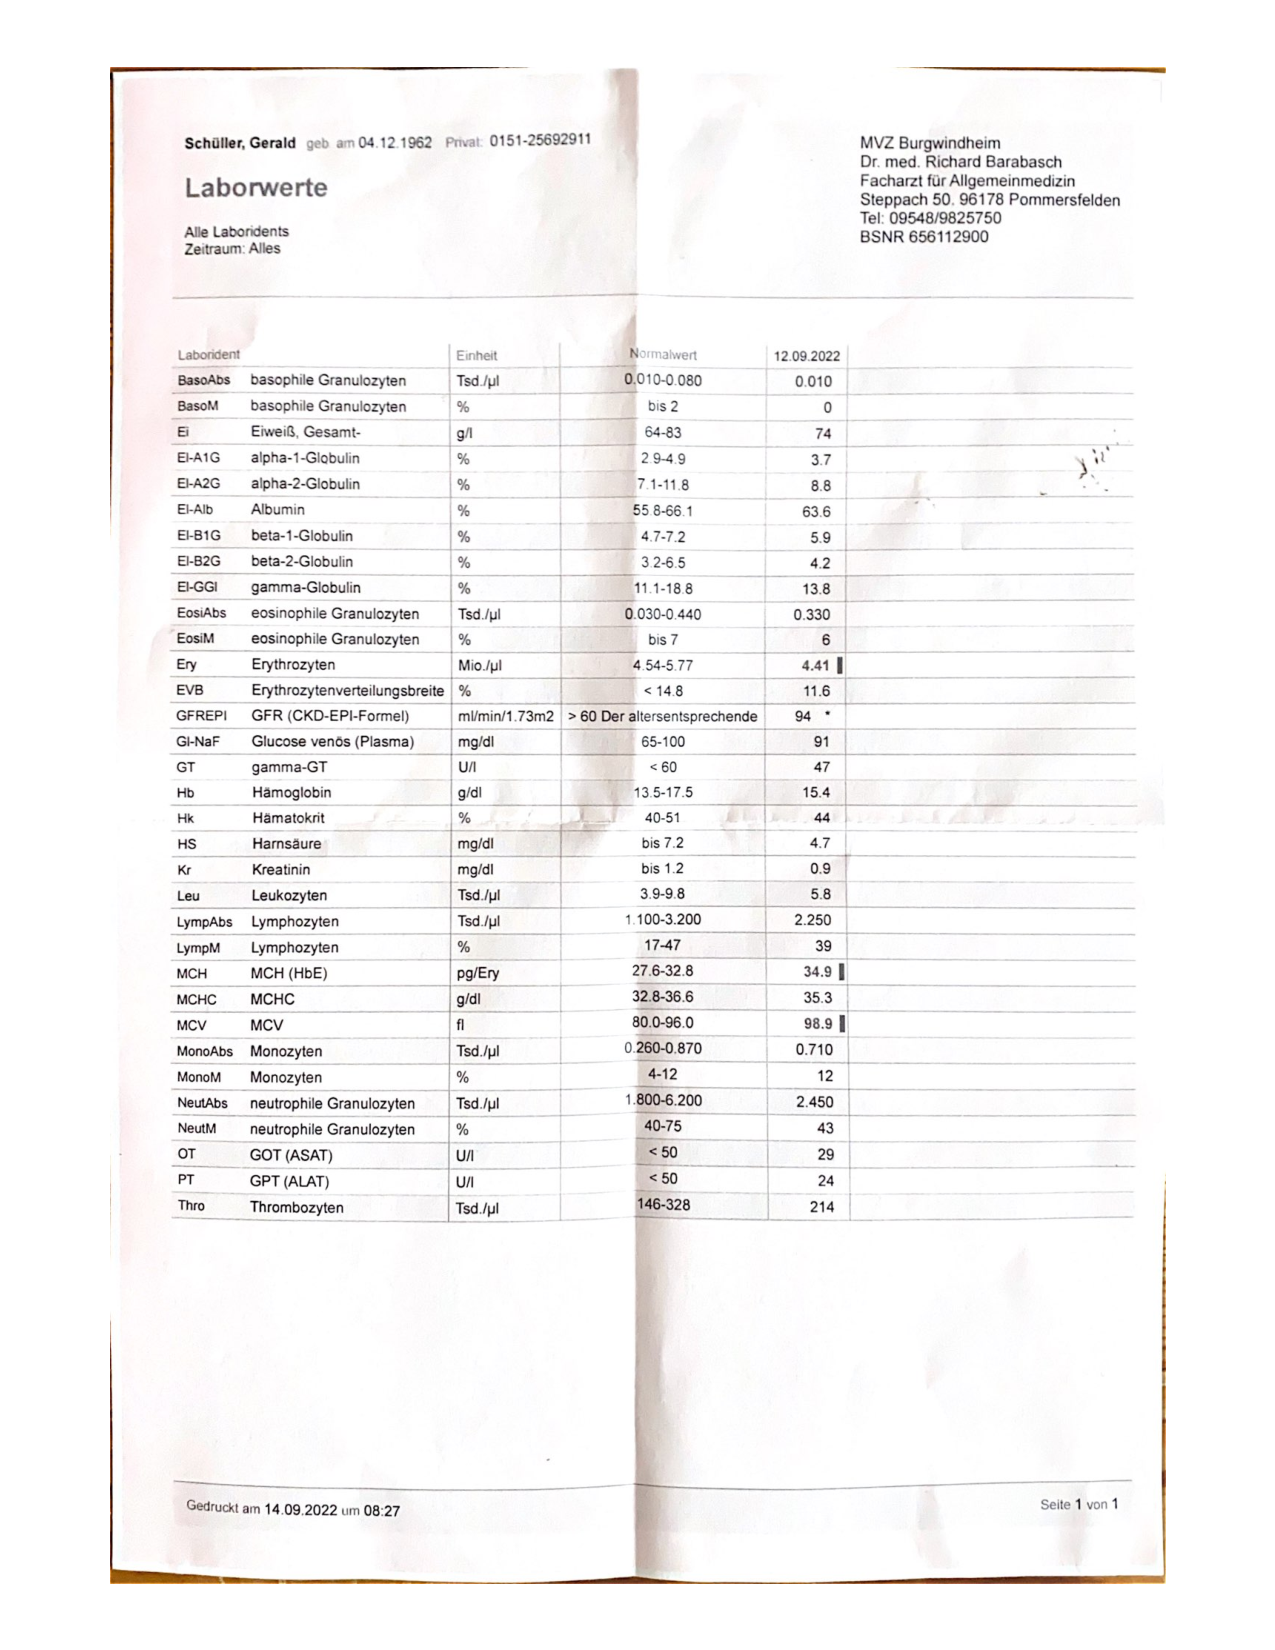
\includepdf[pages=-, scale=0.9, offset=0 0, pagecommand={%
    \begin{flushleft}  
        \section{Appendix}
      \end{flushleft} 
    \subsection{Laborwerte - 12.09.2022}\thispagestyle{plain}}
]{lw220912.pdf}

% Include the next pdf file.
% 
\includepdf[pages=-, scale=0.9, offset=0 0, pagecommand={%
%    \subsection{Ludwig Wittgenstein, Tractatus}\thispagestyle{plain}}
% ]{tractatus.pdf}


% Include the pdf file.
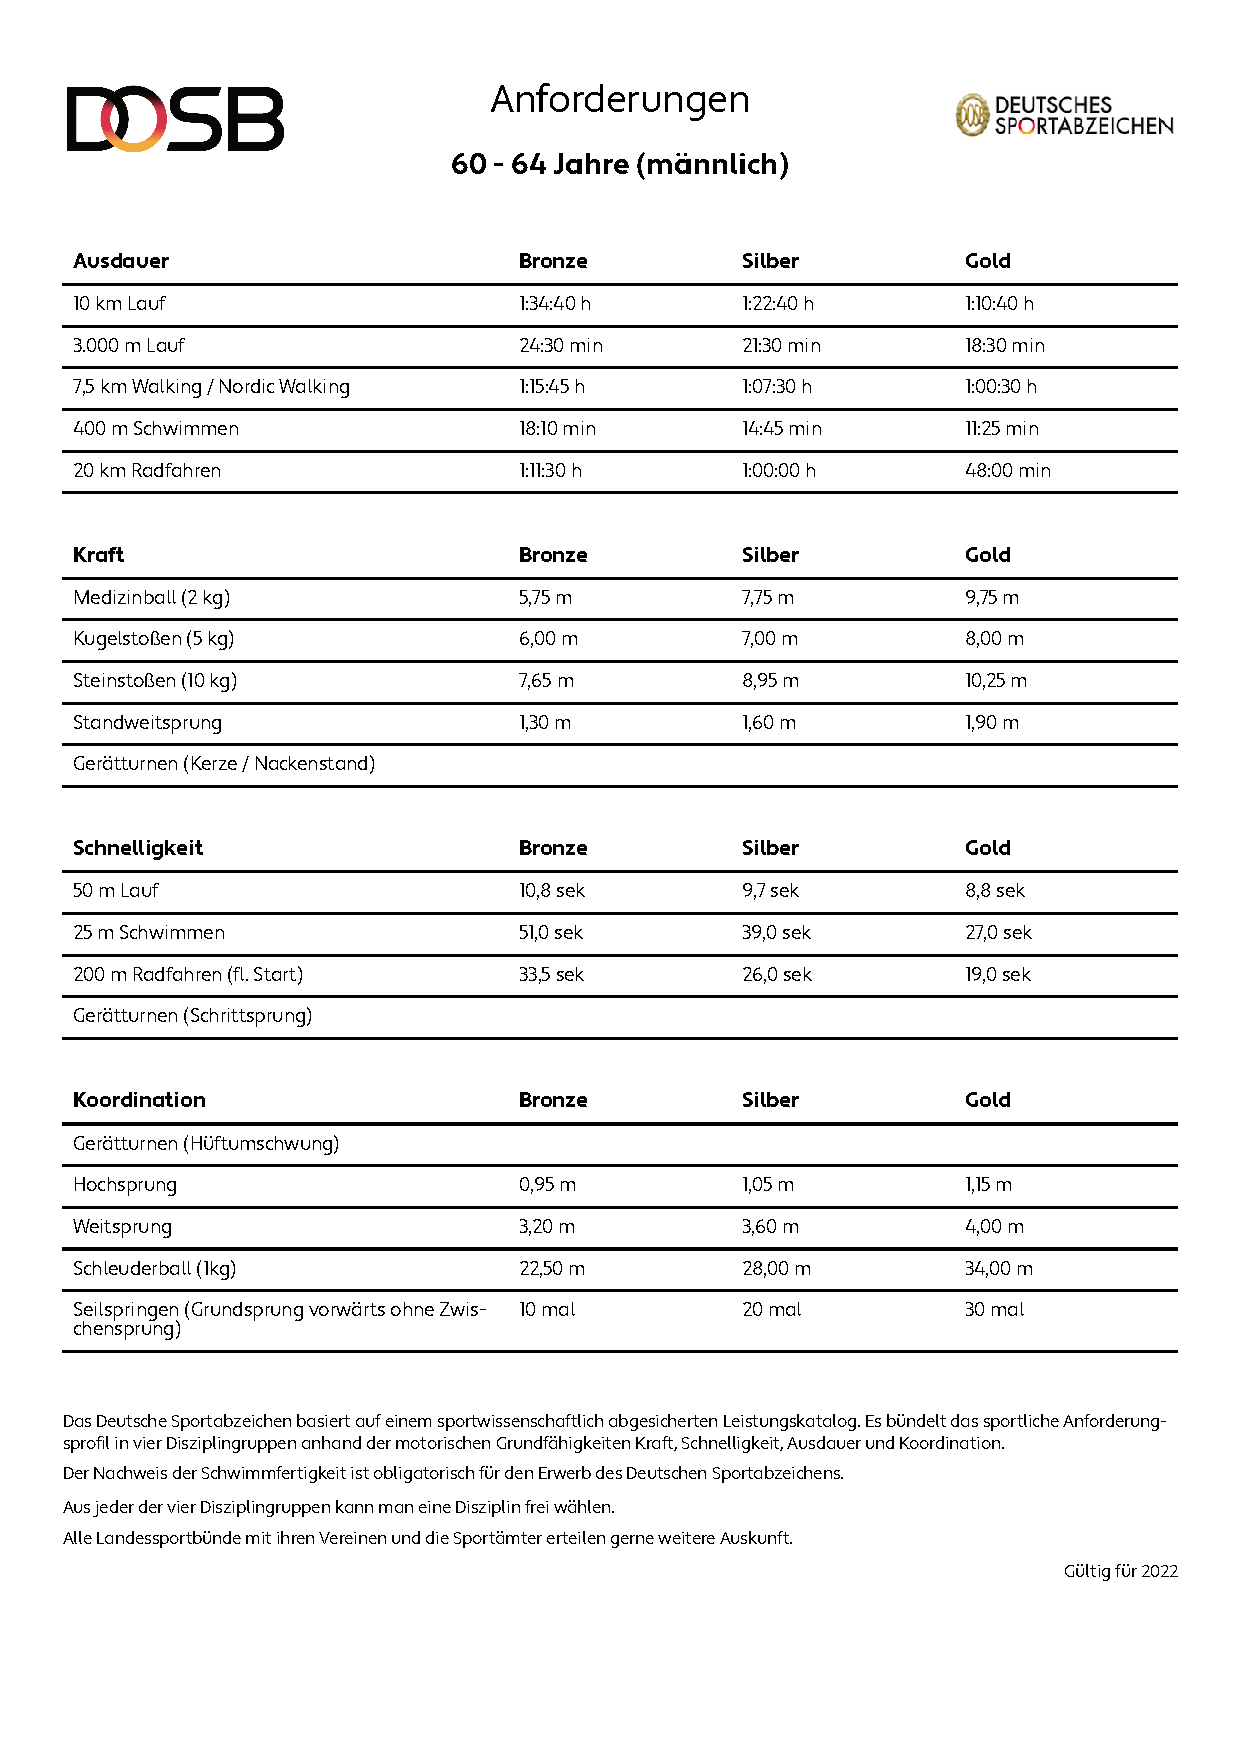
\includepdf[pages=-, scale=0.9, offset=0 0, pagecommand={%
    \subsection{Deutsches Sportabzeichen}\thispagestyle{plain}}
]{dosb.pdf}


\subsection{Saaletalklinik}

\verb+https://saaletal.campus-nes.de/behandlungsangebot/unsere-kliniken/saaletalklinik.html+


\subsubsection{Therapiekonzept}

\verb+https://saaletal.campus-nes.de/fileadmin/user_upload/Therapiekonzept_Saaletalklinik_2014.pdf+


\subsubsection{Körper}

{\bf Morgen} \\
Seife, 6 Zahnbürsten, 3 Tuben Zahnpasta, 1 kleines Handtuch, Haarbürste, Haargel, Parfüm

\vskip 4pt
{\bf Duschen} \\
Rasierhalter, Rasierklingen, 3 Flaschen Shampoo, 3 grosse Handtücher


\subsubsection{Kleidung}

\vskip 4pt
{\bf Sport} \\
Einlegesohlen, 2 Ganituren Trainingskleidung


\vskip 4pt
{\bf Schwimmen} \\
Badetasche, Badehose, Schwimmbrille

\vskip 4pt
{\bf Alltag} \\
4 Zimmermanshosen, 8 Unterhosen, 8 Paar Socken, 8 T-Shirts, 4 Pullover


\subsubsection{Sport}

Zazen-Matte, Zazen-Sitzkissen, Schal, Liegestützgriffe, Roller, Knieschoner


\subsubsection{Bücher}

Tractatus


\subsubsection{Informatik}

aWatch, aWatch-Ladekabel, iPhone, iPhone-Ladekabel, iPad, iPad-Ladekabel,
Computer, Bildschirm, Tastatur


\subsection{Menübilder}

\verb+cd menue; mogrify -format png vleber.jpeg+ \\
\verb+cd menue; mogrify -format png eleber.jpeg+ \\
\verb+cd menu; gthumb vleber.png+

\vskip 4pt
\verb+https://tex.stackexchange.com/questions/234441/latex-includegraphics-width-and-height+


\subsubsection{Thunfisch mit Spinat-Ravioli}

\begin{figure}[H] % <-- Use [H] for exactly here
  
% \centering
\parbox{4cm}{
  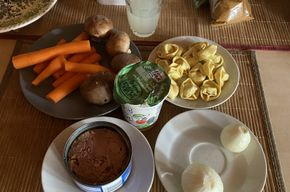
\includegraphics[
    width=4cm,
    height=3cm,
    keepaspectratio,
  ]{menue/vThunfischR.png}
\caption{Vorbereitung}}
\qquad
\begin{minipage}{4cm}
  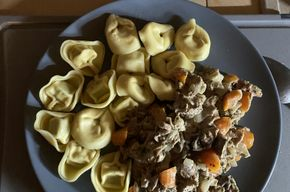
\includegraphics[
    width=4cm,
    height=3cm,
    keepaspectratio,
  ]{menue/eThunfischR.png}
\caption{Ergebnis}

\end{minipage}
\end{figure}


\subsubsection{Leber mit Bohnen}

\begin{figure}[H] % <-- Use [H] for exactly here
  
% \centering
\parbox{4cm}{
  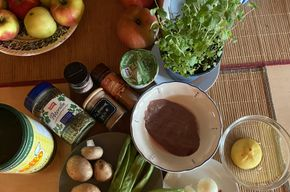
\includegraphics[
    width=4cm,
    height=3cm,
    keepaspectratio,
  ]{menue/vLeberBohnen.png}
\caption{Vorbereitung}}
\qquad
\begin{minipage}{4cm}
  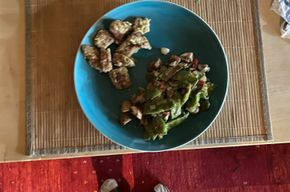
\includegraphics[
    width=4cm,
    height=3cm,
    keepaspectratio,
  ]{menue/eLeberBohnen.png}
\caption{Ergebnis}

\end{minipage}
\end{figure}


\subsubsection{Tofu mit Kartoffeln}

\begin{figure}[H] % <-- Use [H] for exactly here
  
% \centering
\parbox{4cm}{
  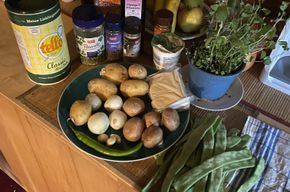
\includegraphics[
    width=4cm,
    height=3cm,
    keepaspectratio,
  ]{menue/vTofuKartoffeln.png}
\caption{Vorbereitung}}
\qquad
\begin{minipage}{4cm}
  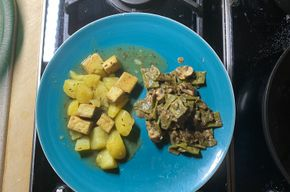
\includegraphics[
    width=4cm,
    height=3cm,
    keepaspectratio,
  ]{menue/eTofuKartoffeln.png}
\caption{Ergebnis}

\end{minipage}
\end{figure}


\subsubsection{Leber mit Kohlrabi}

\begin{figure}[H] % <-- Use [H] for exactly here
  
% \centering
\parbox{4cm}{
  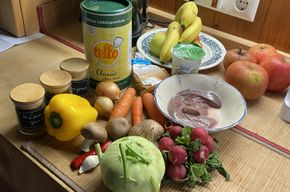
\includegraphics[
    width=4cm,
    height=3cm,
    keepaspectratio,
  ]{menue/vLeberKohlrabi.png}
\caption{Vorbereitung}}
\qquad
\begin{minipage}{4cm}
  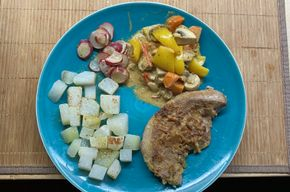
\includegraphics[
    width=4cm,
    height=3cm,
    keepaspectratio,
  ]{menue/eLeberKohlrabi.png}
\caption{Ergebnis}

\end{minipage}
\end{figure}


\subsubsection{Wiener mit Sauerkraut}

\begin{figure}[H] % <-- Use [H] for exactly here
  
% \centering
\parbox{4cm}{
  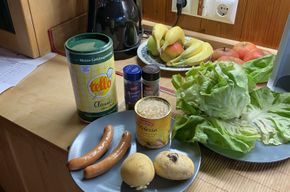
\includegraphics[
    width=4cm,
    height=3cm,
    keepaspectratio,
  ]{menue/vWienerSk.png}
\caption{Vorbereitung}}
\qquad
\begin{minipage}{4cm}
  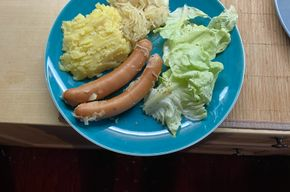
\includegraphics[
    width=4cm,
    height=3cm,
    keepaspectratio,
  ]{menue/eWienerSk.png}
\caption{Ergebnis}

\end{minipage}
\end{figure}


\subsubsection{Thunfisch mit Mohrrüben}

\begin{figure}[H] % <-- Use [H] for exactly here
  
% \centering
\parbox{4cm}{
  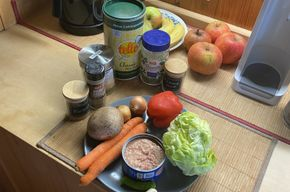
\includegraphics[
    width=4cm,
    height=3cm,
    keepaspectratio,
  ]{menue/vThunfischMr.png}
\caption{Vorbereitung}}
\qquad
\begin{minipage}{4cm}
  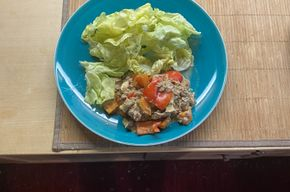
\includegraphics[
    width=4cm,
    height=3cm,
    keepaspectratio,
  ]{menue/eThunfischMr.png}
\caption{Ergebnis}

\end{minipage}
\end{figure}


\subsection{iPhone 1}

\verb+https://de.wikipedia.org/wiki/IPhone+ \\
\verb+https://de.wikipedia.org/wiki/IPhone_(1._Generation)+ \\
\verb+https://appleinsider.com/articles/07/07/02/+ \\
\verb+iphone_video_teardown_reveals_samsung_intel_balda_design_wins.html+ \\
\verb+https://www.zdnet.com/article/infineon-a-big-winner-in-iphone-teardown/+

  % Initialize the note counter.
  \setcounter{notec}{0}

  \notep 4 Vorschule, Nimmersatt und Pippi will ich verwenden für die Geschichte
  von iPhone-1.

  \vskip 2pt
  Wo und wann habt ihr mit der Entwicklung angefangen?

  \vskip 2pt
  Wahrscheinlich 2005 im Südwestpark.

  \vskip 2pt
  Eigentlich will ich erstmal was malen, vielleicht mein Opus-Board
  (Vorschule: Male genau aus.)

  \vskip 2pt
  Mit wem hast du zusammengearbeitet?

  \vskip 2pt
  Herbert, Astrid und Gerhard. Die Geschichte mit: Für meinen Freund Herbert (Nimmersatt 1)

  \vskip 2pt
  Mit Pippi will ich weitermachen (Pippi 7 - 15).

  \vskip 2pt
  Die Zeit ist fast um.

  \vskip 2pt
  Dann vielleicht morgen.


  {\bf 25.10.2022}
  
  % Initialize the note counter.
  \setcounter{notec}{0}

  \notep 4 Form und Farbe: \\
  1. Das Opus-Board ist rechteckig und grün (Vorschule 1). \\
  2. {\prop {???}} (Vorschule 2).

  \notep 4 Bild und Elementarsätze: \\
  1. Nachts, im Neonlich, lag auf dem Tisch eine kleine Plastikkarte
  (Nimmersatt 2).

  \notep 4 Sätze und Wahrheit: \\
  1. Neben dem Kanal in der grossen Stadt steht ein Betonblock mit Büros
  (Pippi 7 - 15). \\
  2. {\prop {???}} (Pippi 16 - 19).
  
\subsection{Lua}

\verb+https://www.lua.org/+

\vskip 4pt
\verb+sudo apt-get install lua5.3+


\subsubsection{Lua 5.3 Reference Manual}

\verb+https://www.lua.org/manual/5.3/+


\subsubsection{Emacs Lua Mode}

\verb+https://github.com/immerrr/lua-mode+

\vskip 4pt
To fetch the list of packages you can do \\
\verb+    <M-x> package-refresh-contents+

\vskip 4pt
And after that lua-mode can be installed with \\
\verb+    <M-x> package-install "lua-mode"+


\subsubsection{Tutorial}

\verb+http://edu-9.de/uploads/documents/lua_tutorial.pdf+ \\
\verb+https://riptutorial.com/Download/lua.pdf+


\subsubsection{Syntax Highlighting}

\begin{minted}{tex}
\usepackage{minted}         % Syntax highlighting: \begin{minted}{lua}.
\end{minted}

% Start of the syntax highlighting.
\begin{minted}{lua}
-- This is single line comment
--
print("Hello World!");
\end{minted}
% The syntax highlighting ends her.


\subsection{Charaktereigenschaften}

\verb+https://wortwuchs.net/charaktereigenschaften/+

abenteuerlustig \\
abergläubisch \\
abwesend \\
aggressiv \\
aktiv \\
analytisch \\
angriffslustig \\
ängstlich \\
anspruchsvoll \\
anstrengend \\
antriebslos \\
aufdringlich \\
aufgeregt \\
aufgeweckt \\
auflehnend \\
aufmerksam \\
ausdauernd \\
ausweichend \\
begeistert \\
begierig \\
begriffsstutzig \\
belastbar \\
bequem \\
besserwisserisch \\
beweglich \\
bissig \\
differenziert \\
dünnhäutig \\
durchtrieben \\
effizient \\
ehrgeizig \\
eingeschüchtert \\
einsam \\
einzelgängerisch \\
elitär \\
empfindlich \\
entscheidungsfreudig \\
entschlossen \\
ernst \\
exakt \\
fatalistisch \\
fleißig \\
flexibel \\
fokussierend \\
frech \\
freundlich
gedankenverloren \\
geduldig \\
gehemmt \\
gierig \\
größenwahnsinnig \\
grüblerisch \\
gründlich \\
harmlos \\
hinterfotzig \\
höflich \\
innovativ \\
instinktiv \\
interessiert \\
intuitiv \\
ironisch \\
jähzornig \\
kämpferisch \\
kalkulierend \\
klug \\
kompliziert \\
konsequent \\
konstruktiv \\
konzentriert \\
leichtsinnig \\
leistungsbereit \\
lernwillig \\
lethargisch \\
lösungsorientiert \\
menschenscheu \\
methodisch \\
mimosenhaft \\
misstrauisch \\
motiviert \\
mutig \\
nachdenklich \\
naiv \\
nervös \\
neugierig \\
niedergeschlagen \\
optimistisch \\
pingelig \\
pragmatisch \\
raffiniert \\
realistisch \\
reflektierend \\
religiös \\
schreckhaft \\
selbständig \\
schüchtern \\
selbstreflektierend \\
selbstüberschätzend \\
skeptisch \\
sorgfältig \\
spirituell \\
sportlich \\
sprunghaft \\
steif \\
still \\
stolz \\
strukturiert \\
tagträumerisch \\
träumerisch \\
überempfindlich \\
unsicher \\
verklemmt \\
verlässlich \\
verunsichert \\
verträumt \\
verwahrlost \\
wankelmütig \\
willensstark \\
wortkarg \\
zäh \\
zielorientiert \\
zuverlässig


\newpage
% xxx
% Start of the library.
%

% Print the complete library.
\nocite{*}

\printbibheading


\printbibliography[keyword=Philosophie, heading=subbibliography,
  title={Philosophie}]


\printbibliography[keyword=Buddhismus, heading=subbibliography,
  title={Buddhismus}]


\printbibliography[keyword=AA, heading=subbibliography,
  title={Anonyme Alkoholiker}]


\printbibliography[keyword=Computer, heading=subbibliography,
  title={Computer}]


\printbibliography[keyword=Erzählungen, heading=subbibliography,
  title={Erzählungen}]


\printbibliography[keyword=Romane, heading=subbibliography,
  title={Romane}]


\printbibliography[keyword=Theater, heading=subbibliography,
  title={Theatestücke}]


\printbibliography[keyword=Musik, heading=subbibliography,
  title={Musik}]


\printbibliography[keyword=Bilder, heading=subbibliography,
  title={Bilderbücher}]


\printbibliography[keyword=Kindergeschichten, heading=subbibliography,
  title={Kindergeschichten}]


\printbibliography[keyword=Vorschule, heading=subbibliography,
  title={Vorschule}]


\printbibliography[keyword=Schule, heading=subbibliography,
  title={Schulbücher}]


\printbibliography[keyword=Evolution, heading=subbibliography,
  title={Evolution}]


\newpage
\subsection{Recherche}

\subsubsection{Tractatus}

{\bf 17.10.2022} \\
4.24 Den Elementarsatz schreibe ich als Funktion der Namen in der Form:
$f(x)$, $\varphi (x,y)$, etc. \\
Oder ich deute ihn durch die Buchstaben $p$, $q$, $r$ an.

\vskip 4pt
{\bf 18.10.2022} \\
4.3 Die Wahrheitsmöglichkeiten der Elementarsätze bedeuten die Möglichkeiten des
Bestehens und Nichtbestehens der Sachverhalte.

\vskip 4pt
{\bf 23.10.2022} \\
4.431 Der Ausdruck der Übereinstimmung und Nichtübereinstimmung mit den
Wahrheitsmöglichkeiten der Elementarsätze drückt die Wahrheitsbedingungen des
Satzes aus. \\
Der Satz ist der Ausdruck seiner Wahrheitsbedingungen.

\vskip 4pt
{\bf 25.10.2022} \\
4.52 $\ldots$ (So könnte man in gewissem Sinne sage, dass {\it alle} Sätze
Verallgemeinerungen der Elementarsätze sind.)


\subsubsection{Basis Bibel}

{\bf 17.10.2022} \\
4.1.13 Sie zwangen sie mit Gewalt zur Arbeit \\
und machten ihnen das Leben zur Qual.

\vskip 4pt
{\bf 18.10.2022} \\
4.2.5 Da kam die Tochter des Pharao zum Baden an den Nil.

\vskip 4pt
{\bf 23.10.2022} \\
5.14.26 Darauf sagte der HERR zu Mose: ,,Strecke die Hand aus über das Meer! Das
Wasser soll über die Ägypter zurückfluten - über ihre Streitwagen und über ihre
Reiter.''

\vskip 4pt
{\bf 25.10.2022} \\
6.19.20 So stieg der HERR auf den Berg Sinai herab, auf den Gipfel des Berges.


\subsubsection{Buddhas Lehrreden}

{\bf 17.10.2022} \\
Sutra über das Glück (18 - 20): \\
Die Möglichkeit zum Lernen haben, \\
im Beruf oder Handwerk geschickt sein \\
und wissen, wie man die Richtlinien und liebevolle Rede praktiziert - \\
das ist das größte Glück.

\vskip 4pt
{\bf 18.10.2022} \\
Sutra über Thera den Älteren (21 - 22): \\
$\ldots$, dass es einen ganz hervorragenden Weg gib, allein zu sein. Das ist der
Weg der eingehenden Betrachtung; $\ldots$ Er ermöglicht uns, in aller Muße im
gegenwärtigen Augenblick zu weilen, frei von Begehren.

\vskip 4pt
{\bf 23.10.2022} \\
Sutra über die Kenntnis vom besseren Weg, allein zu leben (23 - 25): \\
$\ldots$ und denkt: $>$ Dieser Körper, das bin ich. Ich bin dieser Körper. Diese
Gefühle, das bin ich. Ich bin diese Gefühle. Diese Wahrnehmungen, das bin ich.
Ich bin diese Wahrnehmungen. Diese geistigen Gebilde, das bin ich. Ich bin diese
geistigen Gebilde. Diese Bewusstsein, das bin ich. Ich bin dieses
Bewusstsein $<$, dann lässt sich diese Person von der Gegenwart hinwegtreiben.

\vskip 4pt
{\bf 23.10.2022} \\
Sutra über die rechte Anschauung (26 - 30): \\
$\ldots$ Wer das Unheilsame und die Wurzeln des Unheilsamen erkennt, $\ldots$
der hat rechte Anschaung $\ldots$ \\
Die Wurzeln des Unheilsamen sind Gier, Hass und Verblendung.


\newpage
\subsection{Fukanzazengi}

\verb+https://antaiji.org/de/classics/fukanzazengi/+

\vskip 4pt
{\bf Universelle Aufforderung zum Zazen}

\vskip 4pt
Von Beginn an war der Weg vollkommen gegenwärtig, warum sollten wir ihn erst noch üben und bezeugen
müssen? Das Gefährt der Lehre bewegt sich frei und von selbst, welchen Sinn hätte da unser eifriges Üben? Im
ganzen Universum gibt es nicht das geringste Staubkorn, wie könnten wir je versuchen, uns selbst durch die
Übung zu reinigen? An diesem Ort ist alles offenbar, wohin sollten wir die Füße unserer Übung richten?

\vskip 4pt
Wenn du auch nur ein Haarbreit von Unterscheidung machst, wird sich eine Kluft wie zwischen Himmel und Erde
auftun. Wenn du dem einen folgst und dem anderen widerstrebst, wird dein Geist wie Pulver vom Wind verweht.
Auch wenn du stolz auf dein Wissen und deine große Erleuchtung bist, auch wenn deine intuitive Weisheit Buddha
erschaut hat und du den Weg erlangt und den Geist geklärt hast, selbst wenn deine entschlossene Gesinnung zum
Himmel durchbricht: Selbst dann zappelst du nur so wie einer, der mit dem Kopf in der Schale feststeckt, während
der Leib den Ausweg zum Leben fast vollkommen vergessen hat.

\vskip 4pt
Shakyamuni wurde als Weiser geboren. Dennoch saß er für sechs Jahre im Gion-Park. Siehst du seine Spuren
nicht? Bodhidharma brachte das Siegel des Geistes aus Indien. Hörst du nicht das Echo der neun Jahre, die er im
Shorin-Tempel gegen die Wand gerichtet saß? Wenn es selbst bei den Alten so war, wie könnten wir Heutigen uns
da vor der Übung drücken? Suche nicht nach Buchstaben, verstricke dich nicht in Worte, lass endlich ab von
deinen Kommentaren. Dreh’ das Licht um und beleuchte dich selbst, lerne, einen Schritt zurück zu tun. Von selbst
werden sich Körper und Geist lösen, dein Urangesicht wird ganz offenbar. Wenn du die Dinge sehen willst, so wie
sie sind, musst du – hier und jetzt – ganz du selbst sein, so wie du bist.

\vskip 4pt
Für die Zenübung ist ein stiller Ort geeignet. Halte Maß beim Essen und Trinken und löse dich aus allen
Bindungen, lasse die zehntausend Angelegenheiten ruhen. Denke nicht an „gut“ und „böse“, urteile nicht über
„richtig“ oder „falsch“. Dein Geist und Bewusstsein drehen sich im Kreis – lass sie zur Ruhe kommen. Hör’ auf alles
mit deinen Gedanken und Meinungen abzuwägen. Versuche auch nicht einen Buddha aus dir zu machen, gib dich
nicht ab mit „Sitzen“ oder „Liegen“.

\vskip 4pt
Breite eine dicke Sitzmatte aus. Darauf lege dein Sitzkissen. Sitze entweder im halben Lotussitz oder im vollen
Lotussitz. Beim vollen Lotussitz lege den rechten Fuß auf den linken Oberschenkel und dann den linken Fuß auf
den rechten Oberschenkel. Beim halben Lotussitz lege einfach den linken Fuß auf den rechten Oberschenkel.

\vskip 4pt
Trage dein Gewand locker und ordentlich. Lege die rechte Hand auf den linken Fuß und die linke Hand auf die
rechte Hand. Die Spitzen der beiden Daumen sind gegeneinander gestützt. Sitze gerade, in der richtigen Haltung.
Sitze nicht nach links oder rechts gekrümmt, vornüber gebeugt oder zurückgelehnt. Ohren und Schultern sollten
in einer Linie sein, während die Nase in einer Linie mit dem Nabel ist. Die Zunge sollte am Gaumen anliegen. Halte
Lippen und Zähne geschlossen und die Augen stets geöffnet. Atme leise durch die Nase.

\vskip 4pt
Ist der Körper auf diese Weise eingestimmt, dann atme einmal tief durch den Mund aus. Schwinge deinen
Oberkörper erst nach links und rechts. Dann sitze reglos wie ein mächtiger Berg in Konzentration und denke auf
dem Grund des Nicht-Denkens. Wie denkt man auf dem Grund des Nicht-Denkens? Es ist die Loslösung vom
Denken (Undenken). Dies macht die Kunst des Zazen aus.

\vskip 4pt
Zazen ist keine Meditationstechnik – es ist das Dharmator großer Zufrieden- und Gelassenheit. Es ist das übende
Erweisen des endlosen Dharmaweges. Hier verwirklicht sich das offenbare Geheimnis, es gibt kein Netz mehr, in
dem du dich verfangen könntest. Wenn du dir dies zu eigen gemacht hast, bist du wie ein Drache, der zurück ins
Wasser taucht, du bist wie ein Tiger, der durch die Berge streift. Die wahre Lehre verwirklicht sich von selbst, und
deine Müdigkeit und Zerstreutheit werden sich auflösen.

\vskip 4pt
Wenn du aus Zazen aufstehst, bewege deinen Körper erst langsam, und richte dich dann in Ruhe auf. Tue es nicht
Hals über Kopf.

\vskip 4pt
Siehe, dass all die, die über das Gewöhliche wie das Ungewöhnliche hinausgehen und im Sitzen wie im Stehen
sterben, sich dieser einen Kraft überlassen. Das gilt auch für den Finger und den Mast, die Nadel und den Schlegel,
mit denen das Rad der Lehre gedreht wurde. Der Erweis, der mit dem Wedel und der Faust, dem Stock und dem
Schrei erbracht wurde, lässt sich durch Gedanken und Urteile nicht verstehen. Wie sollte ihn je einer erkennen,
der sich mit übendem Erweisen um das Erlangen übernatürlicher Kräfte bemüht? Dein Handeln muss sich von
Klang und Gestalt lösen, es muss sich auf die Ordnung gründen, die vor intellektuellem Sehen und Verstehen liegt.

\vskip 4pt
Mache dir keine Gedanken darüber, ob du mehr weißt als die anderen oder nicht. Glaube nicht, dass der Kluge
besser ist als der Dumme. Gib’ dich einfach hin an die Übung: Das ist es, was Beschreiten des Weges genannt wird.
Nichts könnte das übende Erweisen beflecken – sich nach dem Weg zu richten bedeutet, den Alltag zu leben. In
dieser wie in allen anderen Welten, in Indien wie in China, wird das Buddhasiegel auf gleiche Weise bewahrt, und
der Wind der Wahrheit weht frei und ungehindert. Gib’ dich einfach hin an das Sitzen, geh’ auf im unbeweglichen
Zustand des Zazen. Auch wenn es tausend Wege mit zehntausend Unterschieden gibt, beschreite den einen Weg
in dem du einfach nur Zen übst. Welchen Sinn hat es, das Sitzkissen bei dir zuhause zu verlassen, um in der
Fremde umherzuirren? Ein falscher Schritt, und du wirst den Boden unter deinen Füßen verlieren. Als Mensch
geboren, hast du die seltene Gelegenheit den Weg zu gehen – verschwende deine Zeit nicht!

\vskip 4pt
Dem Buddhaweg in diesem Leben begegnet – wie könntest du die Gelegenheit ungenutzt lassen und fliegenden
Funken nachblicken? Dein Leben ist wie das Tau am Gras. Das Schicksal schlägt zu wie ein Blitz. Dein Körper hat
keinen Bestand, in einem Augenblick musst du ihn aufgeben. Ich hoffe, dass du, der du die Lehre so gelernt hast
wie ein Blinder, der an einem Elephanten tastet, nicht in Angst und Schrecken versetzt wirst, wenn du dem
wirklichen Drachen begegnest. Übe den direkten Weg der Wahrheit mit Leib und Seele, respektiere den
Müßiggänger, der jenseits jedes Lernens ist. Teile die Weisheit mit Buddhas und Buddhas, erbe das Samadhi von
Patriarchen und Patriarchen. Auf diese Weise geübt – auf diese Weise verwirklicht. Die Schatzkammer öffnet sich
von 

\newpage
\subsection{Hannya Shingyo}

\verb+http://www.zensplitter.de/Herzsutra.pdf+

\vskip 4pt
{\bf Das Herz der Grossen Transzendenten Weisheit}

\vskip 4pt
So habe ich gehört: Zu einer gewissen Zeit weilte der Erhabene in Rajagriha
auf dem Geierberg, zusammen mit einer großen Anzahl von Mönchen und
Bodhisattvas. Zu dieser Zeit war der Erhabene in Gambhirava-Sambodhi
versunken. Und zur gleichen Zeit dachte der große Bodhisattva
Aryavalokiteshvara, der die tiefe transzendente Weisheit studierte, also: 'Es
gibt fünf geistig-körperliche Daseinserscheinungen, und diese hat er als von
Natur aus leer erachtet'

\vskip 4pt
Da sprach der ehrwürdige Shariputra, veranlasst durch die Kraft des
Erwachten, also: 'Wenn der Sohn oder die Tochter einer Familie das Studium
der tiefen transzendenten Weisheit beginnen wollen, wie sollen sie belehrt
werden?'

\vskip 4pt
Darauf antwortete der große Bodhisattva Aryavalokiteshvara dem ehrwürdigen
Shariputra also: 'Wenn der Sohn oder die Tochter einer Familie das Studium
der tiefen transzendenten Weisheit beginnen wollen, dann müssen sie so
denken:

\vskip 4pt
'Es gibt fünf geistig-körperliche Daseinserscheinungen, und diese hat er als
von Natur aus leer erachtet. Form ist Leere und Leere ist tatsächlich Form.
Leere ist nicht verschieden von Form, Form ist nicht verschieden von Leere.
Was Form ist, das ist Leere, was Leere ist, das ist Form. So sind auch
Wahrnehmung, Empfindung, Begrifflichkeit und Bewusstsein ebenfalls Leere.
So, oh Shariputra, haben alle Dinge den Charakter von Leere; sie haben weder
Anfang noch Ende, sie sind fehlerlos und nicht fehlerlos, sie sind nicht
unvollkommen und nicht vollkommen. Daher, oh Shariputra, gibt es hier in
dieser Leere keine Form, keine Wahrnehmung, keine Empfindung, keine
Begrifflichkeit, kein Bewusstsein. Kein Auge, Ohr, Nase, Zunge, Tastorgan und
Geist. Keine sichtbare Form, kein Klang, Geruch, Geschmack, Tastempfindung
und Objekte im Bewusstsein. Es gibt kein Sehen, Hören, Riechen, Schmecken,
Er- tasten, Erkennen. Es gibt kein Wissen, keine Unwissenheit, keine
Zerstörung von Unwissenheit, es gibt keine Vergänglichkeit und keinen Tod,
keine Aufhebung von Vergänglichkeit und Tod. Das Leiden, der Ursprung des
Leidens, das Ende des Leidens und der Pfad, der zum Ende des Leidens führt,
dies alles existiert nicht. Es gibt kein Wissen, kein Erlangen und kein NichtErlangen von Nirvana. Daher, oh Shariputra, da es kein Erlangen gibt, verweilt
ein Mensch, der sich der transzendenten Weisheit der Bodhisattvas genähert
hat, in der Umhüllung des Bewusstseins. Doch wenn die Umhüllung des
Bewusstseins vernichtet ist, wird er frei von aller Furcht, er ist jenseits von
Unbeständigkeit, er genießt höchstes Nirvana 

\vskip 4pt
Alle Buddhas der Vergangenheit, Gegenwart und Zukunft erwach- ten,
nachdem sie sich der transzendenten Weisheit genähert hatten, zum höchsten,
vollkommenen Wissen.

\vskip 4pt
Daher sollten wir das große Mantra der transzendenten Weisheit kennen, das
Mantra der großen Weisheit, das unübertroffene Mantra, das Mantra, das alles
Leiden stillt - es ist Wahrheit, keine Falschheit - das Mantra zur Erlangung
transzendenter Weisheit:

\vskip 4pt
OM GATE GATE PARAGATE PARASAMGATE BODHI SVAH

\vskip 4pt
gegangen, gegangen, hinübergegangen, erreicht, erwacht

\vskip 4pt
So, oh Shariputra, sollte ein Bodhisattva das Studium der tiefen
transzendenten Weisheit lehren.'

\vskip 4pt
Als dann der Erhabene sich aus seiner Meditation erhob, gab er dem
ehrwürdigen Bodhisattva Avalokiteshvara seine Zustimmung, indem er sagte:
'Wohl getan, wohl getan, edler Sohn! So ist es, edler Sohn. So muss in der Tat
dieses Studium der tiefen transzendenten Weisheit ausgeführt werden. Wie es
von dir beschrieben wurde, findet es den Beifall der heiligen So-Gegangenen.'
So sprach der Erhabene mit freudigem Herzen. Und der ehrwürdige Shariputra,
der geehrte Bodhisattva Avalokiteshvara, die ganze Versammlung und die
Welten der Götter, Menschen, Dämonen und Geister priesen die Worte des
Erhabenen.

\vskip 4pt
Hier endet das Sutra vom Herzen der transzendenten Weisheit.


\newpage
\subsection{Tractatus}

\verb+https://www.mathebibel.de/funktionen+ \\
\verb+https://home.mathematik.uni-freiburg.de/wolke/Schuster_Skript.pdf+ \\
\verb+http://www.fb10.uni-bremen.de/khwagner/grundkurs2/kapitel3.aspx+ \\
\verb+https://ftp.agdsn.de/pub/mirrors/latex/dante/fonts/stix/doc/stix.pdf+


\newpage
\subsection{Märchen und Sagen}

\subsubsection{Das Hirtenbüblein}

\verb+https://de.wikisource.org/wiki/Das_Hirtenb%C3%BCblein_(1857)+

\vskip 4pt
Es war einmal ein Hirtenbübchen, das war wegen seiner weisen Antworten, die es
auf alle Fragen gab, weit und breit berühmt. Der König des Landes hörte auch
davon, glaubte es nicht und ließ das Bübchen kommen. Da sprach er zu ihm
,,kannst du mir auf drei Fragen, die ich dir vorlegen will, Antwort geben, so
will ich dich ansehen wie mein eigen Kind, und du sollst bei mir in meinem
königlichen Schloß wohnen.'' Sprach das Büblein ,,wie lauten die drei Fragen?''
Der König sagte ,,die erste lautet wie viel Tropfen Wasser sind in dem
Weltmeer?'' Das Hirtenbüblein antwortete ,,Herr König, laßt alle Flüsse auf der
Erde verstopfen, damit kein Tröpflein mehr daraus ins Meer lauft, das ich nicht
erst gezählt habe, so will ich euch sagen, wie viel Tropfen im Meere sind.''
Sprach der König ,,die andere Frage lautet wie viel Sterne stehen am Himmel?''
Das Hirtenbübchen sagte ,,gebt mir einen großen Bogen weiß Papier,'' und dann
machte es mit der Feder so viel feine Punkte darauf, daß sie kaum zu sehen und
fast gar nicht zu zählen waren und einem die Augen vergiengen, wenn man darauf
blickte. Darauf sprach es ,,so viel Sterne stehen am Himmel, als hier Punkte auf
dem Papier zählt sie nur.'' Aber niemand war dazu im Stand. Sprach der König
,,die dritte Frage lautet wie viel Secunden hat die Ewigkeit?'' Da sagte das
Hirtenbüblein ,,in Hinterpommern liegt der Demantberg, der hat eine Stunde [284]
in die Höhe, eine Stunde in die Breite und eine Stunde in die Tiefe; dahin kommt
alle hundert Jahr ein Vögelein und wetzt sein Schnäblein daran, und wenn der
ganze Berg abgewetzt ist, dann ist die erste Secunde von der Ewigkeit vorbei.''

\vskip 4pt
Sprach der König ,,du hast die drei Fragen aufgelöst wie ein Weiser und sollst
fortan bei mir in meinem königlichen Schlosse wohnen, und ich will dich ansehen
wie mein eigenes Kind.“

\subsubsection{Frau Holle}

\verb+https://de.wikisource.org/wiki/Frau_Holle_(1857)+

\vskip 4pt
Eine Wittwe hatte zwei Töchter, davon war die eine schön und fleißig, die andere
häßlich und faul. Sie hatte aber die häßliche und faule, weil sie ihre rechte
Tochter war, viel lieber, und die andere mußte alle Arbeit thun und der
Aschenputtel im Hause sein. Das arme Mädchen mußte sich täglich auf die große
Straße bei einem Brunnen setzen, und mußte so viel spinnen, daß ihm das Blut aus
den Fingern sprang. Nun trug es sich zu, daß die Spule einmal ganz blutig war,
da bückte es sich damit in den Brunnen und wollte sie abwaschen: sie sprang ihm
aber aus der Hand und fiel hinab. Es weinte, lief zur Stiefmutter und erzählte
ihr das Unglück. Sie schalt es aber so heftig und war so unbarmherzig, daß sie
sprach ,,hast du die Spule hinunterfallen lassen, so hol sie auch wieder herauf.''
Da gieng das Mädchen zu dem Brunnen zurück und wußte nicht was es anfangen
sollte: und in seiner Herzensangst sprang es in den Brunnen hinein, um die Spule
zu holen. Es verlor die Besinnung, und als es erwachte und wieder zu sich selber
kam, war es auf einer schönen Wiese wo die Sonne schien und viel tausend Blumen
standen. Auf dieser Wiese gieng es fort und kam zu einem Backofen, der war
voller Brot; das Brot aber rief ,,ach, zieh mich raus, zieh mich raus, sonst
verbrenn ich: ich bin schon längst ausgebacken.'' Da trat es herzu, und holte
mit dem Brotschieber alles nach einander heraus. Danach gieng es weiter und kam
zu einem Baum, der hieng voll Äpfel, und rief ihm zu ,,ach schüttel mich,
schüttel mich, wir Äpfel sind alle mit einander reif.'' Da schüttelte es den
Baum, daß die Äpfel fielen als regneten sie, und schüttelte bis keiner mehr oben
war; und als es alle in einen Haufen zusammengelegt hatte, gieng es wieder
weiter. Endlich kam es zu einem kleinen Haus, daraus guckte eine alte Frau,
weil sie aber so große Zähne hatte, ward ihm angst, und es wollte fortlaufen.
Die alte Frau aber rief ihm nach ,,was fürchtest du dich, liebes Kind? bleib bei
mir, wenn du alle Arbeit im Hause ordentlich thun willst, so soll dirs gut gehn.
Du mußt nur Acht geben daß du mein Bett gut machst und es fleißig aufschüttelst,
daß die Federn fliegen, dann schneit es in der Welt; ich bin die Frau Holle.''
Weil die Alte ihm so gut zusprach, so faßte sich das Mädchen ein Herz, willigte
ein und begab sich in ihren Dienst. Es besorgte auch alles nach ihrer
Zufriedenheit, und schüttelte ihr das Bett immer gewaltig auf daß die Federn wie
Schneeflocken umher flogen; dafür hatte es auch ein gut Leben bei ihr, kein
böses Wort, und alle Tage Gesottenes und Gebratenes. Nun war es eine Zeitlang
bei der Frau Holle, da ward es traurig und wußte anfangs selbst nicht was ihm
fehlte, endlich merkte es daß es Heimweh war; ob es ihm hier gleich viel
tausendmal besser gieng als zu Haus, so hatte es doch ein Verlangen dahin.
Endlich sagte es zu ihr ,,ich habe den Jammer nach Haus kriegt, und wenn es mir
auch noch so gut hier unten geht, so kann ich doch nicht länger bleiben, ich muß
wieder hinauf zu den Meinigen.'' Die Frau Holle sagte ,,es gefällt mir, daß du
wieder nach Haus verlangst, und weil du mir so treu gedient hast, so will ich
dich selbst wieder hinauf bringen.'' Sie nahm es darauf bei der Hand und führte
es vor ein großes Thor. Das Thor ward aufgethan, und wie das Mädchen gerade
darunter stand, fiel ein gewaltiger Goldregen, und alles Gold blieb an ihm
hängen, so daß es über und über davon bedeckt war. ,,Das sollst du haben, weil
du so fleißig gewesen bist'' sprach die Frau Holle und gab ihm auch die Spule
wieder, die ihm in den Brunnen gefallen war. Darauf ward das Thor verschlossen,
und das Mädchen befand sich oben auf der Welt, nicht weit von seiner Mutter
Haus: und als es in den Hof kam, saß der Hahn auf dem Brunnen und rief

\vskip 4pt
,,kikeriki, \\
unsere goldene Jungfrau ist wieder hie.''

\vskip 4pt
Da gieng es hinein zu seiner Mutter, und weil es so mit Gold bedeckt ankam, ward
es von ihr und der Schwester gut aufgenommen.

\vskip 4pt
Das Mädchen erzählte alles, was ihm begegnet war, und als die Mutter hörte wie
es zu dem großen Reichthum gekommen war, wollte sie der andern häßlichen und
faulen Tochter gerne dasselbe Glück verschaffen. Sie mußte sich an den Brunnen
setzen und spinnen; und damit ihre Spule blutig ward, stach sie sich in die
Finger und stieß sich die Hand in die Dornhecke. Dann warf sie die Spule in den
Brunnen und sprang selber hinein. Sie kam, wie die andere, auf die schöne Wiese
und gieng auf demselben Pfade weiter. Als sie zu dem Backofen gelangte, schrie
das Brot wieder ,,ach, zieh mich raus, zieh mich raus, sonst verbrenn ich, ich
bin schon längst ausgebacken.'' Die Faule aber antwortete ,,da hätt ich Lust
mich schmutzig zu machen,'' und gieng fort. Bald kam sie zu dem Apfelbaum, der
rief ,,ach, schüttel mich, schüttel mich, wir Äpfel sind alle mit einander reif.''
Sie antwortete aber ,,du kommst mir recht, es könnte mir einer auf den Kopf
fallen,'' und gieng damit weiter. Als sie vor der Frau Holle Haus kam, fürchtete
sie sich nicht, weil sie von ihren großen Zähnen schon gehört hatte, und
verdingte sich gleich zu ihr. Am ersten Tag that sie sich Gewalt an, war fleißig
und folgte der Frau Holle, wenn sie ihr etwas sagte, denn sie dachte an das
viele Gold, das sie ihr schenken würde; am zweiten Tag aber fieng sie schon an
zu faullenzen, am dritten noch mehr, da wollte sie Morgens gar nicht aufstehen.
Sie machte auch der Frau Holle das Bett nicht wie sichs gebührte, und schüttelte
es nicht, daß die Federn aufflogen. Das ward die Frau Holle bald müde und sagte
ihr den Dienst auf. Die Faule war das wohl zufrieden und meinte nun würde der
Goldregen kommen; die Frau Holle führte sie auch zu dem Thor, als sie aber
darunter stand, ward statt des Goldes ein großer Kessel voll Pech ausgeschüttet.
,,Das ist zur Belohnung deiner Dienste'' sagte die Frau Holle und schloß das
Thor zu. Da kam die Faule heim, aber sie war ganz mit Pech bedeckt, und der Hahn
auf dem Brunnen, als er sie sah, rief

\vskip 4pt
,,kikeriki, \\
unsere schmutzige Jungfrau ist wieder hie.''

\vskip 4pt
Das Pech aber blieb fest an ihr hängen und wollte, so lange sie lebte, nicht
abgehen.

\subsubsection{Der Arme und der Reiche}

\verb+https://de.wikisource.org/wiki/Der_Arme_und_der_Reiche_(1857)+

\vskip 4pt
Vor alten Zeiten, als der liebe Gott noch selber auf Erden unter den Menschen
wandelte, trug es sich zu, daß er eines Abends müde war und ihn die Nacht
überfiel, bevor er zu einer Herberge kommen konnte. Nun standen auf dem Weg vor
ihm zwei Häuser einander gegenüber, das eine groß und schön, das andere klein
und ärmlich anzusehen, und gehörte das große einem Reichen, das kleine einem
armen Manne. Da dachte unser Herr Gott ,,dem Reichen werde ich nicht
beschwerlich fallen: bei ihm will ich übernachten.'' Der Reiche, als er an seine
Thüre klopfen hörte, machte das Fenster auf und fragte den Fremdling was er
suche? Der Herr antwortete ,,ich bitte um ein Nachtlager.'' Der Reiche guckte
den Wandersmann von Haupt bis zu den Füßen an, und weil der liebe Gott schlichte
Kleider trug und nicht aussah wie einer, der viel Geld in der Tasche hat,
schüttelte er mit dem Kopf und sprach ,,ich kann euch nicht aufnehmen, meine
Kammern liegen voll Kräuter und Samen, und sollte ich einen jeden beherbergen,
der an meine Thüre klopft, so könnte ich selber den Bettelstab in die Hand
nehmen. Sucht euch anderswo ein Auskommen.'' Schlug damit sein Fenster zu und
ließ den lieben Gott stehen. Also kehrte ihm der liebe Gott den Rücken und gieng
hinüber zu dem kleinen Haus. Kaum hatte er angeklopft, so klinkte der Arme schon
sein Thürchen auf und bat den Wandersmann einzutreten. ,,Bleibt die Nacht über
bei mir,'' sagte er ,,es ist schon finster, und heute könnt ihr doch nicht weiter
kommen.'' Das gefiel dem lieben Gott und er trat zu ihm ein. Die Frau des Armen
reichte ihm die Hand, hieß ihn willkommen und sagte er möchte sichs bequem
machen und vorlieb nehmen, sie hätten nicht viel, aber was es wäre, gäben sie
von Herzen gerne. Dann setzte sie Kartoffeln ans Feuer, und derweil sie kochten,
melkte sie ihre Ziege, damit sie ein wenig Milch dazu hätten. Und als der Tisch
gedeckt war, setzte sich der liebe Gott nieder und aß mit ihnen, und schmeckte
ihm die schlechte Kost gut, denn es waren vergnügte Gesichter dabei. Nachdem sie
gegessen hatten, und Schlafenszeit war, rief die Frau heimlich ihren Mann und
sprach ,,hör, lieber Mann, wir wollen uns heute Nacht eine Streu machen, damit
der arme Wanderer sich in unser Bett legen und ausruhen kann: er ist den ganzen
Tag über gegangen, da wird einer müde.'' ,,Von Herzen gern,'' antwortete er,
,,ich wills ihm anbieten,'' gieng zu dem lieben Gott und bat ihn, wenns ihm
recht wäre, möcht er sich in ihr Bett legen und seine Glieder ordentlich
ausruhen. Der liebe Gott wollte den beiden Alten ihr Lager nicht nehmen, aber
sie ließen nicht ab, bis er es endlich that und sich in ihr Bett legte: sich
selbst aber machten sie eine Streu auf die Erde. Am andern Morgen standen sie
vor Tag schon auf und kochten dem Gast ein Frühstück, so gut sie es hatten. Als
nun die Sonne durchs Fensterlein schien und der liebe Gott aufgestanden war, aß
er wieder mit ihnen und wollte dann seines Weges ziehen. Als er in der Thüre
stand, kehrte er sich um und sprach ,,weil ihr so mitleidig und fromm seid, so
wünscht euch dreierlei, das will ich euch erfüllen.'' Da sagte der Arme ,,was
soll ich mir sonst wünschen als die ewige Seligkeit, und daß wir zwei, so lang
wir leben, gesund dabei bleiben und unser nothdürftiges tägliches Brot haben;
fürs dritte weiß ich mir nichts zu wünschen.'' Der liebe Gott sprach ,,willst
du dir nicht ein neues Haus für das alte wünschen?'' ,,O ja,'' sagte der Mann,
,,wenn ich das auch noch erhalten kann, so wär mirs wohl lieb.'' Da erfüllte der
Herr ihre Wünsche, verwandelte ihr altes Haus in ein neues, gab ihnen nochmals
seinen Segen und zog weiter.

\vskip 4pt
Es war schon voller Tag, als der Reiche aufstand. Er legte sich ins Fenster und
sah gegenüber ein neues, reinliches Haus mit rothen Ziegeln, wo sonst eine alte
Hütte gestanden hatte. Da machte er große Augen, rief seine Frau herbei und
sprach ,,sag mir, was ist geschehen? Gestern Abend stand noch die alte elende
Hütte, und heute steht da ein schönes neues Haus. Lauf hinüber und höre wie das
gekommen ist.'' Die Frau gieng und fragte den Armen aus: er erzählte ihr
,,gestern Abend kam ein Wanderer, der suchte Nachtherberge, und heute Morgen
beim Abschied hat er uns drei Wünsche gewährt, die ewige Seligkeit, Gesundheit
in diesem Leben und das nothdürftige tägliche Brot dazu und zuletzt noch statt
unserer alten Hütte ein schönes neues Haus'' Die Frau des Reichen lief eilig
zurück und erzählte ihrem Manne wie alles gekommen war. Der Mann sprach ,,ich
möchte mich zerreißen und zerschlagen: hätt ich das nur gewußt! der Fremde ist
zuvor hier gewesen und hat bei uns übernachten wollen, ich habe ihn aber
abgewiesen.'' ,,Eil dich,'' sprach die Frau, ,,und setze dich auf dein Pferd,
so kannst du den Mann noch einholen, und dann mußt du dir auch drei Wünsche
gewähren lassen.''

\vskip 4pt
Der Reiche befolgte den guten Rath, jagte mit seinem Pferd davon und holte den
lieben Gott noch ein. Er redete fein und lieblich und bat er möchts nicht übel
nehmen, daß er nicht gleich wäre eingelassen worden, er hätte den Schlüssel zur
Hausthüre gesucht, derweil wäre er weggegangen: wenn er des Weges zurück käme,
müßte er bei ihm einkehren. ,,Ja,'' sprach der liebe Gott, ,,wenn ich einmal
zurückkomme, will ich es thun.'' Da fragte der Reiche ob er nicht auch drei
Wünsche thun dürfte, wie sein Nachbar? Ja, sagte der liebe Gott, das dürfte er
wohl, es wäre aber nicht gut für ihn, und er sollte sich lieber nichts
wünschen. Der Reiche meinte er wollte sich schon etwas aussuchen, das zu seinem
Glück gereiche, wenn er nur wüßte, daß es erfüllt würde. Sprach der liebe Gott
,,reit heim, und drei Wünsche, die du thust, die sollen in Erfüllung gehen.''

\vskip 4pt
Nun hatte der Reiche was er verlangte, ritt heimwärts und fieng an nachzusinnen
was er sich wünschen sollte. Wie er sich so bedachte und die Zügel fallen ließ,
fieng das Pferd an zu springen, so daß er immerfort in seinen Gedanken gestört
wurde und sie gar nicht zusammen bringen konnte. Er klopfte ihm an den Hals und
sagte ,,sei ruhig, Liese,'' aber das Pferd machte aufs neue Männerchen. Da ward
er zuletzt ärgerlich und rief ganz ungeduldig ,,so wollt ich, daß du den Hals
zerbrächst!'' Wie er das Wort ausgesprochen hatte, plump, fiel er auf die Erde,
und lag das Pferd todt und regte sich nicht mehr; damit war der erste Wunsch
erfüllt. Weil er aber von Natur geizig war, wollte er das Sattelzeug nicht im
Stich lassen, schnitts ab, hiengs auf seinen Rücken, und mußte nun zu Fuß gehen.
,,Du hast noch zwei Wünsche übrig'' dachte er und tröstete sich damit. Wie er
nun langsam durch den Sand dahin gieng, und zu Mittag die Sonne heiß brannte,
wards ihm so warm und verdrießlich zu Muth: der Sattel drückte ihn auf den
Rücken, auch war ihm noch immer nicht eingefallen, was er sich wünschen sollte.
,,Wenn ich mir auch alle Reiche und Schätze der Welt wünsche,'' sprach er zu
sich selbst, ,,so fällt mir hernach noch allerlei ein, dieses und jenes, das
weiß ich im voraus: ich wills aber so einrichten, daß mir gar nichts mehr übrig
zu wünschen bleibt.'' Dann seufzte er und sprach ,,ja, wenn ich der bairische
Bauer wäre, der auch drei Wünsche frei hatte, der wußte sich zu helfen, der
wünschte sich zuerst recht viel Bier, und zweitens so viel Bier als er trinken
könnte, und drittens noch ein Faß Bier dazu.'' Manchmal meinte er jetzt hätte
er es gefunden, aber hernach schiens ihm doch zu wenig. Da kam ihm so in die
Gedanken was es seine Frau jetzt gut hätte, die säße daheim in einer kühlen
Stube und ließe sichs wohl schmecken. Das ärgerte ihn ordentlich, und ohne daß
ers wußte, sprach er so hin ,,ich wollte die säße daheim auf dem Sattel, und
könnte nicht herunter, statt daß ich ihn da auf meinem Rücken schleppe.'' Und
wie das letzte Wort aus seinem Munde kam, so war der Sattel von seinem Rücken
verschwunden, und er merkte daß sein zweiter Wunsch auch in Erfüllung gegangen
war. Da ward ihm erst recht heiß, er fieng an zu laufen und wollte sich daheim
ganz einsam in seine Kammer hinsetzen und auf etwas Großes für den letzten
Wunsch sinnen. Wie er aber ankommt und die Stubenthür aufmacht, sitzt da seine
Frau mittendrin auf dem Sattel und kann nicht herunter, jammert und schreit. Da
sprach er ,,gib dich zufrieden, ich will dir alle Reichthümer der Welt herbei
wünschen, nur bleib da sitzen.'' Sie schalt ihn aber einen Schafskopf und sprach
,,was helfen mir alle Reichthümer der Welt, wenn ich auf dem Sattel sitze; du
hast mich darauf gewünscht, du mußt mir auch wieder herunter helfen.'' Er mochte
wollen oder nicht, er mußte den dritten Wunsch thun, daß sie vom Sattel ledig
wäre und herunter steigen könnte; und der Wunsch ward alsbald erfüllt. Also
hatte er nichts davon als Ärger, Mühe, Scheltworte und ein verlornes Pferd: die
Armen aber lebten vergnügt, still und fromm bis an ihr seliges Ende.

\subsubsection{Rumpelstilzchen}

\verb+https://de.wikisource.org/wiki/Rumpelstilzchen_(1857)+

\vskip 4pt
Es war einmal ein Müller, der war arm, aber er hatte eine schöne Tochter. Nun
traf es sich, daß er mit dem König zu sprechen kam, und um sich ein Ansehen zu
geben, sagte er zu ihm ,,ich habe eine Tochter, die kann Stroh zu Gold spinnen.''
Der König sprach zum Müller ,,das ist eine Kunst, die mir wohl gefällt, wenn
deine Tochter so geschickt ist, wie du sagst, so bring sie Morgen in mein
Schloß, da will ich sie auf die Probe stellen.'' Als nun das Mädchen zu ihm
gebracht ward, führte er es in eine Kammer, die ganz voll Stroh lag, gab ihr Rad
und Haspel und sprach ,,jetzt mache dich an die Arbeit, und wenn du diese Nacht
durch bis morgen früh dieses Stroh nicht zu Gold versponnen hast, so mußt du
sterben.'' Darauf schloß er die Kammer selbst zu, und sie blieb allein darin.

\vskip 4pt
Da saß nun die arme Müllerstochter und wußte um ihr Leben keinen Rath: sie
verstand gar nichts davon, wie man Stroh zu Gold spinnen konnte, und ihre Angst
ward immer größer, daß sie endlich zu weinen anfieng. Da gieng auf einmal die
Thüre auf, und trat ein kleines Männchen herein und sprach ,,guten Abend,
Jungfer Müllerin, warum weint sie so sehr?'' ,,Ach,'' antwortete das Mädchen,
,,ich soll Stroh zu Gold spinnen, und verstehe das nicht.'' Sprach das Männchen
,,was gibst du mir, wenn ich dirs spinne?'' ,,Mein Halsband'' sagte das Mädchen.
Das Männchen nahm das Halsband, setzte sich vor das Rädchen, und schnurr,
schnurr, schnurr, dreimal gezogen, war die Spule voll. Dann steckte es eine
andere auf, und schnurr, schnurr, schnurr, dreimal gezogen, war auch die zweite
voll: und so giengs fort bis zum Morgen, da war alles Stroh versponnen, und alle
Spulen waren voll Gold. Bei Sonnenaufgang kam schon der König und als er das
Gold erblickte, erstaunte er und freute sich, aber sein Herz ward nur noch
goldgieriger. Er ließ die Müllerstochter in eine andere Kammer voll Stroh
bringen, die noch viel größer war, und befahl ihr das auch in einer Nacht zu
spinnen, wenn ihr das Leben lieb wäre. Das Mädchen wußte sich nicht zu helfen
und weinte, da gieng abermals die Thüre auf, und das kleine Männchen erschien
und sprach ,,was gibst du mir, wenn ich dir das Stroh zu Gold spinne?'' ,,Meinen
Ring von dem Finger'' antwortete das Mädchen. Das Männchen nahm den Ring, fieng
wieder an zu schnurren mit dem Rade und hatte bis zum Morgen alles Stroh zu
glänzendem Gold gesponnen. Der König freute sich über die Maßen bei dem Anblick,
war aber noch immer nicht Goldes satt, sondern ließ die Müllerstochter in eine
noch größere Kammer voll Stroh bringen und sprach ,,die mußt du noch in dieser
Nacht verspinnen: gelingt dirs aber, so sollst du meine Gemahlin werden.''
,,Wenns auch eine Müllerstochter ist,'' dachte er, ,,eine reichere Frau finde
ich in der ganzen Welt nicht.'' Als das Mädchen allein war, kam das Männlein
zum drittenmal wieder und sprach ,,was gibst du mir, wenn ich dir noch diesmal
das Stroh spinne?'' ,,Ich habe nichts mehr, das ich geben könnte'' antwortete
das Mädchen. ,,So versprich mir, wenn du Königin wirst, dein erstes Kind.''
,,Wer weiß wie das noch geht'' dachte die Müllerstochter und wußte sich auch in
der Noth nicht anders zu helfen; sie versprach also dem Männchen was es
verlangte, und das Männchen spann dafür noch einmal das Stroh zu Gold. Und als
am Morgen der König kam und alles fand wie er gewünscht hatte, so hielt er
Hochzeit mit ihr, und die schöne Müllerstochter ward eine Königin.

\vskip 4pt
Über ein Jahr brachte sie ein schönes Kind zur Welt und dachte gar nicht mehr an
das Männchen: da trat es plötzlich in ihre Kammer und sprach ,,nun gib mir was
du versprochen hast.'' Die Königin erschrack und bot dem Männchen alle
Reichthümer des Königreichs an, wenn es ihr das Kind lassen wollte: aber das
Männchen sprach ,,nein, etwas lebendes ist mir lieber als alle Schätze der Welt.''
Da fieng die Königin so an zu jammern und zu weinen, daß das Männchen Mitleiden
mit ihr hatte: ,,drei Tage will ich dir Zeit lassen,'' sprach er, ,,wenn du bis
dahin meinen Namen weißt, so sollst du dein Kind behalten.''

\vskip 4pt
Nun besann sich die Königin die ganze Nacht über auf alle Namen, die sie jemals
gehört hatte, und schickte einen Boten über Land, der sollte sich erkundigen
weit und breit was es sonst noch für Namen gäbe. Als am andern Tag das Männchen
kam, fieng sie an mit Caspar, Melchior, Balzer, und sagte alle Namen, die sie
wußte, nach der Reihe her, aber bei jedem sprach das Männlein ,,so heiß ich
nicht.'' Den zweiten Tag ließ sie in der Nachbarschaft herumfragen wie die Leute
da genannt würden, und sagte dem Männlein die ungewöhnlichsten und seltsamsten
Namen vor, ,,heißt du vielleicht Rippenbiest oder Hammelswade oder Schnürbein?''
aber es antwortete immer ,,so heiß ich nicht.'' Den dritten Tag kam der Bote
wieder zurück und erzählte ,,neue Namen habe ich keinen einzigen finden können,
aber wie ich an einen hohen Berg um die Waldecke kam, wo Fuchs und Has sich gute
Nacht sagen, so sah ich da ein kleines Haus, und vor dem Haus brannte ein Feuer,
und um das Feuer sprang ein gar zu lächerliches Männchen, hüpfte auf einem Bein
und schrie

\vskip 4pt
,,heute back ich, morgen brau ich, \\
übermorgen hol ich der Königin ihr Kind; \\
ach, wie gut ist daß niemand weiß \\
daß ich Rumpelstilzchen heiß!''

\vskip 4pt
Da könnt ihr denken wie die Königin froh war, als sie den Namen hörte, und als
bald hernach das Männlein herein trat und fragte ,,nun, Frau Königin, wie heiß
ich?'' fragte sie erst ,,heißest du Kunz?'' ,,Nein.'' ,,Heißest du Heinz?''
,,Nein.''

\vskip 4pt
,,Heißt du etwa Rumpelstilzchen?''

\vskip 4pt
,,Das hat dir der Teufel gesagt, das hat dir der Teufel gesagt'' schrie das
Männlein und stieß mit dem rechten Fuß vor Zorn so tief in die Erde, daß es bis
an den Leib hineinfuhr, dann packte es in seiner Wuth den linken Fuß mit beiden
Händen und riß sich selbst mitten entzwei.


\subsubsection{Sisyphos}

\verb+https://hekaya.de/sagen/sisyphos--sagen_griechisch_26.html+

\vskip 4pt
So mild und hilfsbereit Götter auch den leidenden Menschen zur Seite treten,
hart und unnachsichtig trifft die rächende Strafe jeden, der ihnen die Stirn
zu bieten wagt.

\vskip 4pt
Für seinen Trotz musste Sisyphos büßen, der Erbauer der herrlichen Stadt
Korinth. Er hielt sich für den listigsten der Sterblichen und scheute sich
deshalb nicht, des Göttervaters Zorn auf sich zu ziehen.

\vskip 4pt
Als Zeus die liebliche Nymphe Aigina entführte, verriet Sisyphos ihn aus
schnödem Eigennutz dem Vater der Geraubten, dem Flussgott Asopos, der ihm dafür
aber versprechen musste, in der Felsenburg der Stadt Korinth eine Quelle
entstehen zu lassen.

\vskip 4pt
In seinem Unwillen zögerte Zeus nicht, den Verwegenen zu bestrafen. Thanatos,
der Tod, erhielt den Auftrag, den Korintherkönig in den Hades zu führen.

\vskip 4pt
Sisyphos wusste jedoch den ungebetenen Sendboten des Göttervaters zu überlisten
und legte ihn in Fesseln, so dass niemand auf Erden mehr sterben konnte, bis
Ares kam. Er befreite den Todesgott, der den fürwitzigen König nun ins Reich der
Schatten führte.

\vskip 4pt
Indessen wusste Sisyphos mit neuer List seiner Haft im Totenreich zu entgehen.
Ehe er in die Unterwelt hinabstieg, hatte er der Gattin streng untersagt, seiner
abgeschiedenen Seele die Totenopfer darzubringen. Daher ließen sich Hades und
Persephone schließlich bereden, ihn noch einmal zu beurlauben, um auf diese
Weise die säumige Gattin an ihre Pflicht zu mahnen.

\vskip 4pt
Der arglistige Sisyphos dachte aber nicht daran, in die Unterwelt
zurückzukehren, und lebte wieder wie vorher unbekümmert und in Freuden.

\vskip 4pt
Doch Zeus' Geduld war nun endgültig erschöpft. Wiederum sandte er den Thanatos,
und diesmal half dem König keine noch so klug erdachte List. Während er beim
üppigen Mahle saß, kam der Tod, und unerbittlich wurde Sisyphos in die Unterwelt
geschleppt.

\vskip 4pt
Dort traf ihn die Strafe. Einen schweren Marmorstein musste er mit großer
Kraftanstrengung einen Hügel hinaufwälzen. Sobald er glaubte, das Ziel erreicht
zu haben, entglitt der tückische Stein seinen Händen und rollte den Hang
hinunter in die Tiefe. Immer wieder musste Sisyphos unter unsäglichen Mühen ans
Werk gehen, doch immer wieder blieb ihm der Erfolg versagt.


\newpage
\subsection{Zensus}

\subsubsection{Bibliographie}

\verb+https://www.zensus2022.de/DE/Was-ist-der-Zensus/_inhalt.html+

\subsubsection{Definitionen}

\begin{mdframed}[style=daystyle, leftmargin=-25pt]
  \begin{itemize}
    \setlength\itemsep{-3pt}
  \item {\emps {Zensus}} 2022 findet in Deutschland wieder ein Zensus statt. Mit
    dieser statistischen Erhebung wird ermittelt, wie viele Menschen in
    Deutschland leben, wie sie wohnen und arbeiten.
  \end{itemize}
\end{mdframed}

\subsubsection{Anmeldung}

\begin{labeling}{Anzahl der Wohnungen:}
  \setlength\itemsep{-3pt}
\item[Zugangsnummer:]        4032 7571 6347
\item[Atkivierungscode:]     5u9j99mh6wg
\item[Anschrift:]            Ich bin Eigentümer
\item[Gebäude:]              Wohngebäude 
\item[Anzahl der Wohnungen:] 1
\item[Fertigstellung:]       2011
\item[Gebäudetyp:]           Freistehendes Einfamilienhaus
\item[Eigentümer:]           Privatpersion
\item[Heizungsart:]          Zentralheizung
\item[Energieträger:]        Holz
\item[Wohnungsnutzung:]      Vom Eigentümer bewohnt
\item[Anzahl der Personen:]  2
\item[Namen:]                Schüller Gerald, Schleicher Renate
\item[Wohnfläche:]           128 $m^2$
\item[Anzahl der Räume:]     6
\item[Weitere Wohngebäude:]  Nein
\end{labeling}

\subsection{Grundsteuer}

\subsubsection{Bibliographie}

\verb+https://de.wikipedia.org/wiki/Grundsteuer+ \\
\verb+https://www.bundesfinanzministerium.de/Content/DE/FAQ/faq-die-neue-grundsteuer.html+ \\
\verb+https://www.elster.de/eportal/start+

\subsubsection{Definitionen}

\begin{mdframed}[style=daystyle, leftmargin=-25pt]
  \begin{itemize}
    \setlength\itemsep{-3pt}
  \item {\emps {Grundsteuer}} (Bodenzins) ist eine Geldleistung für ein
    Eigentum an einem Teil der Erdoberfläche, das im Grundbuch beschrieben wird.
  \end{itemize}
\end{mdframed}

\subsubsection{Grundsteuererklärung}

\begin{enumerate}[label={\Square}]
    \setlength\itemsep{-3pt}
  
  \item [\XBox] Das Dokument muss ich bis zum 31.10.2022 abgeben.
    
  \item [\XBox] Die Erklärung muss ich elektronisch über das ELSTER-Portal an das
    Finanzamt übermitteln.
    
  \item [\XBox] Ein ELSTER-Zertifikat erhalte ich unter \verb+https://www.elster.de/eportal/start+
    
  \item [\XBox] Für das ELSTER-Login benötige ich eine Zertifikationsdatei und ein Passwort.
    
  \item [\XBox] Zugang bekomme ich mit der steuerlichen Identifikationsnummer: \\
    IdNr.: 62 098 453 150; Benutzername: hozan; Lieblingsbuch: Tractatus
    
  \item [\XBox] Ich erhalte zwei Briefe: Aktivierungs-Code und Abrufcode.
    
  \item [\XBox] Per EMail bestätige ich die Aktivierung meines Benutzerkontos: \\
    Benutzername: hozan; Aktivierungs-ID: 282875961012266960
    
  \item [\XBox] Innerhalb von 14 Tagen schickt mir das Finanzamt den Aktivierungs-Code
    postalisch.
    
  \item [\XBox] Mit dem Aktivierungs-Code kann ich die Registrierung fortsetzen: \\
    Aktivierungs-ID: 282875961012266960 \\
    Aktivierungs-Code: 9UZL-AMTL-M4HJ
    
  \item [\XBox] Zertifikationsdatei erstellen: \\
    Name der Zertifikatsdatei: hozan\_elster\_29.09.2022\_14.32.pfx \\
    Passwort für Login: =Logisch2022

  \item [\XBox] Zertifikatsdatei herunterladen: ~/Download/hozan\_elster\_29.09.2022\_14.32.pfx

  \item [\XBox] Erstmaliges Login - Mein Profil ergänzen: \\
    Steuernummer: 207/684/07526

  \item [\XBox] Benutzerkontoinformationen \\
      Gerald Josef Schüller \\
      Benutzerkonto-ID: 1091780273

      \vskip 4pt
      Registriert am \\
      29.09.2022

      \vskip 4pt
      Identifiziert mit \\
      Identifikationsnummer: 62098453150
      
      \vskip 4pt
      Art des Zertifikats \\
      Persönliches Zertifikat 

      \vskip 4pt
      Gültigkeit des Zertifikats \\
      Gültig bis: 29.09.2025 um 14:36 Uhr

    \item [\XBox] Mein ELSTER: Alle Formulare: Grundsteuer: Grundsteuer für Bayern

    \item Grundsteuer für Bayern \\
      Für das Ausfüllen des Formulars benötigen Sie je nach persönlicher
      Situation unter anderem folgende Informationen:

      \vskip 4pt
      Aktenzeichen Ihres Grundstücks bzw. Ihres Betriebs der Land- und Forstwirtschaft \\
      Flurstücksfläche \\
      Flurstücksnummer \\
      Gebäudefläche

      \vskip 4pt
      Weitere Informationen finden Sie unter www.grundsteuer.bayern.de.

      \vskip 4pt
      Vom 1. Juli 2022 bis zum 31. Dezember 2022 können Sie ausgewählte Daten,
      wie z. B. Flurstücksnummer und amtliche Fläche, aus dem
      Liegenschaftskataster zum Stichtag 1. Januar 2022 kostenlos über das
      Internetportal BayernAtlas-Grundsteuerabrufen. Beim BayernAtlas-Grundsteuer
      handelt es sich um ein Angebot der Bayerischen Vermessungsverwaltung. Sie
      können der Veröffentlichung der Daten zu Ihrem Flurstück im
      BayernAtlas-Grund\-steuer widersprechen:
      
      \vskip 4pt
      \verb+https://www.ldbv.bayern.de/produkte/grundsteuer.html+

\end{enumerate}

% \subsubsection{Aktenzeichen}

% Include the pdf file.
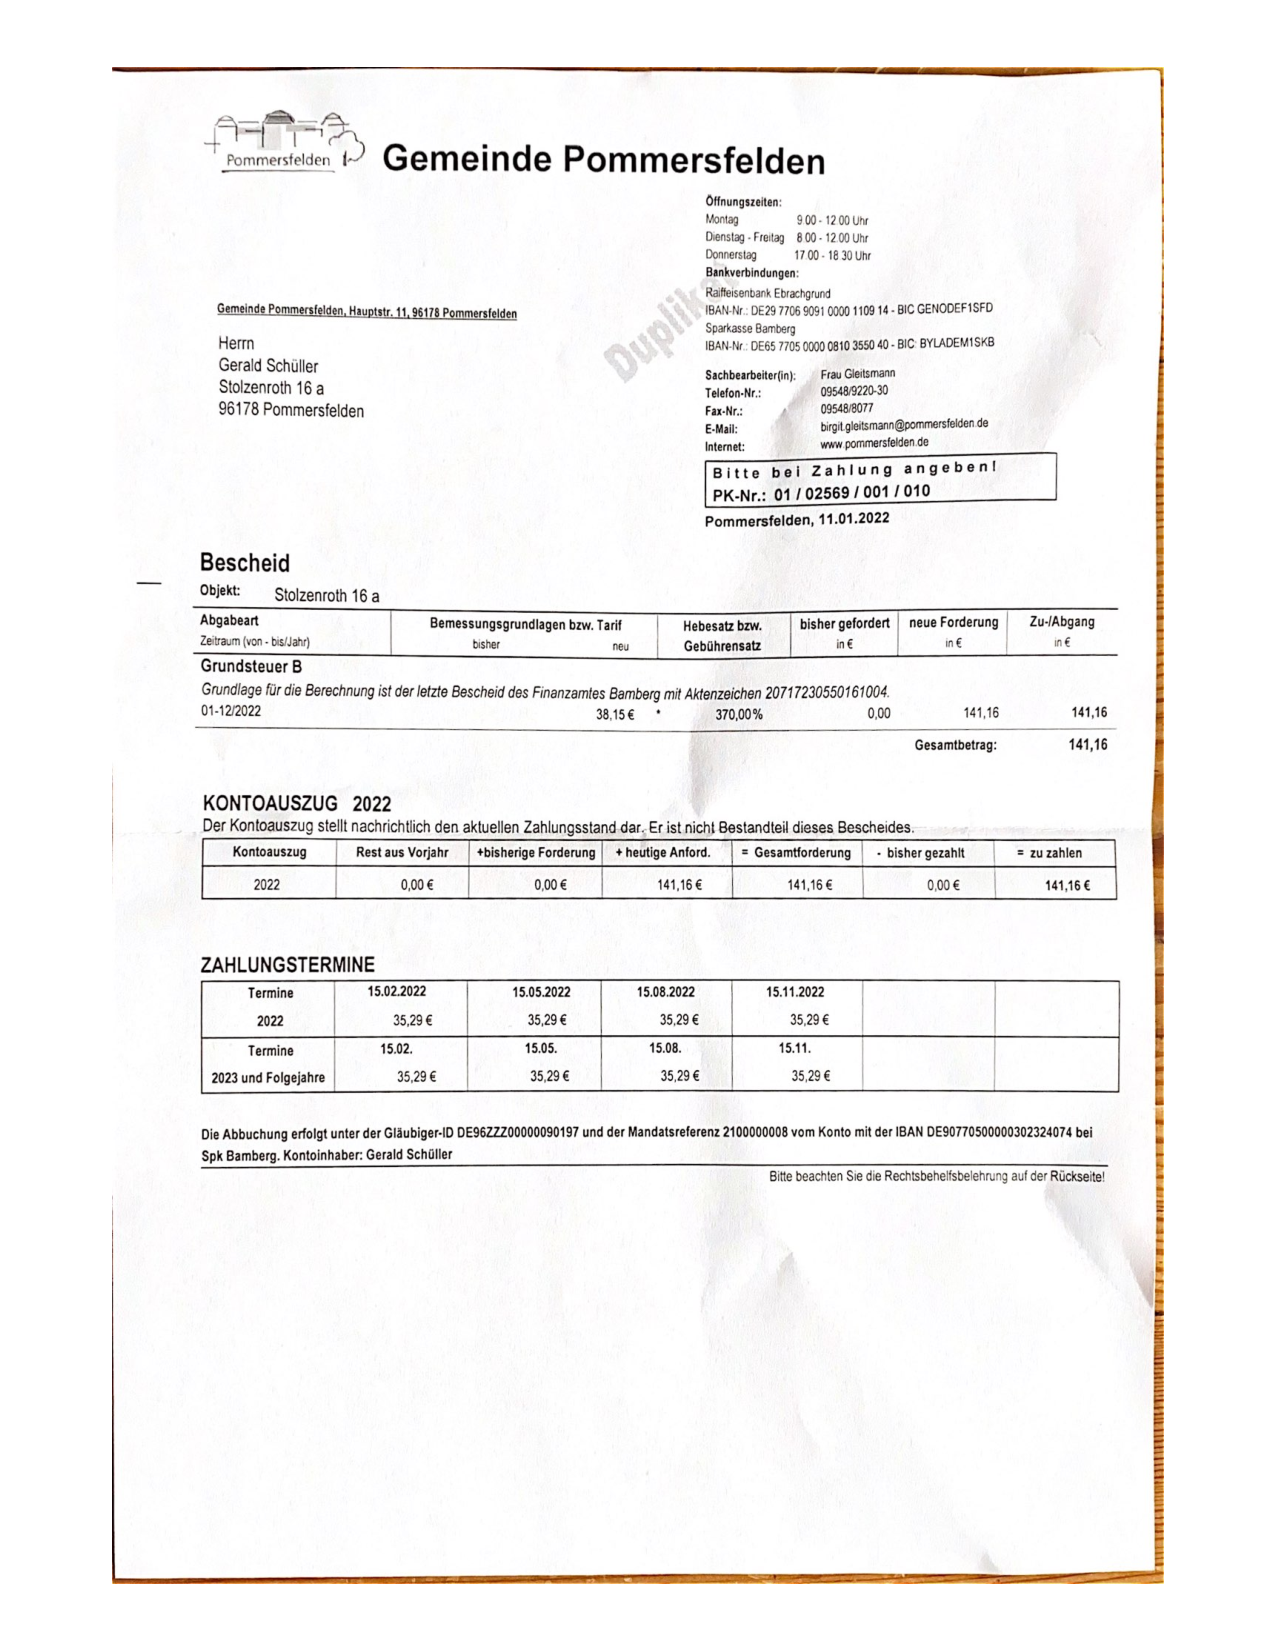
\includepdf[pages=-, scale=0.9, offset=0 0, pagecommand={%
    \begin{flushleft}  
        \subsubsection{Aktenzeichen}
      \end{flushleft} 
    \paragraph{Bescheid}\thispagestyle{plain}}
]{GrstAktz.pdf}


\subsection{Ausblick}

\subsubsection{Muskelaufbau}

\verb+https://www.welt.de/sport/fitness/plus214620124+ \\
\verb+/Fitness-Training-Die-groessten-Fehler-beim-Muskelaufbau.html+

% End of a LaTeX text, that is to be printed.
\end{document}
